\batchmode
\documentclass[a4paper]{article}
\usepackage{a4wide}
\usepackage{makeidx}
\usepackage{fancyhdr}
\usepackage{graphicx}
\usepackage{multicol}
\usepackage{float}
\usepackage{textcomp}
\usepackage{alltt}
\usepackage{times}
\usepackage[utf8]{inputenc}
\usepackage{doxygen}
\makeindex
\setcounter{tocdepth}{3}
\renewcommand{\footrulewidth}{0.4pt}
\begin{document}
\begin{titlepage}
\vspace*{7cm}
\begin{center}
{\Large libbpm \\[1ex]\large 0.3 }\\
\vspace*{1cm}
{\large Generated by Doxygen 1.5.6}\\
\vspace*{0.5cm}
{\small Wed Jun 25 17:31:48 2008}\\
\end{center}
\end{titlepage}
\pagenumbering{roman}
\tableofcontents
\pagenumbering{arabic}
\section{libbpm}
\label{index}\begin{Desc}
\item[Author:]Bino Maiheu, University College London 

Mark Slater, University of Cambridge 

Alexey Lyapin, University College London 

Stewart Boogert, Royal Holloway University of London\end{Desc}
\subsection{Introduction}\label{main_main_intro}
libbpm is a C-library which contains low level beam position monitor (BPM) signal processing routines. It's aim is to form a complete set of routines needed to handle RF Cavity BPM data, from digital downmixing, sampling, calibrating analysing and simulating BPM data. This library has been developed in the context of the BPM work done by the accelerator physics groups at University College London, Royal Holloway University of London and the University of Cambridge (UK) (2006-2007)

The library consists out of a set of submodules which take care of different parts of the BPM signal handling. There are modules for BPM processing, calibration, simulation, general waveform handling, some numerical routines, memory management etc...

The library is licenced under the \doxyref{GNU General Public License v2.}{p.}{licence_gpl}\subsection{Documentation structure}\label{main_main_docu}
The documentation for this library is generated using doyxygen. For each module the documentation is contained in it's respective header file :

\begin{itemize}
\item \doxyref{The waveform handling module}{p.}{group__wave_wave}\item \doxyref{The digital signal processing module}{p.}{group__dsp_dsp}\item \doxyref{The BPM processing module}{p.}{group__processing}\end{itemize}
\subsection{Compilation}\label{main_main_compile}
The compilation of the libbpm structure is defined using the GNU autotools. Therefore making it portable under most unix flavours and MacOS as well as windows ( see futher ).\subsubsection{Compilation under Linux/Unix/MacOS}\label{main_main_compile_unix}
For compilation under any unix flavour, please execute the standart sequence of {\tt }./configure , {\tt make}, and {\tt make} install. The default options for the configure script apply.

If you have extracted the library from CVS, then you will have to generate the build scripts. the {\tt autogen.sh} script takes care of that. Run it and afterwards you can simply execute the same steps as above.\subsubsection{Note on Compilation under Windows}\label{main_main_compile_win32}
This is a remnant from libespec, need to retest this and write proper documentation on it, but for what it's worth... here goes :

To compile libbpm under windows, it is best to use the MinGW + MSYS environment which enables one to build native libraries under windows (dll). For this you need to declare some routines during the build process using the dllexport macro that MinGW defines. So when you want to compile this library as a DLL, set the BUILD\_\-DLL define statement active below. Or compile using -DBUILD\_\-DLL. When you want to use this headerfile to for linking with the bpm.ddl library, undefine the BUILD\_\-DLL, this will enable the compiler to import routines from libbpm in other programs from the ddl. Under linux it does not make a difference as the if statement checks first for the existence of the DLL\_\-EXPORT and \_\-\_\-WIN32\_\-\_\- macros.\subsection{Using libbpm in your programs}\label{main_main_usage}
libbpm is a standalone plain C library. Care has been taken to not have to use special compiler options e.g. the library avoids having to be C99 compliant by implementing it's own complex data type, rounding function etc.. So it should be fairly portable to most platforms.

To use libbpm in your makefiles for your project, a convenient script has been created which automatically gives you the correct compiler options and library locations. See this makefile example on how to use the script {\tt libbpm-config} 



\begin{Code}\begin{verbatim}    #Example makefile that uses libbpm and ROOT (hey.. why not :D !)

    SRC         = main.cpp subroutine.cpp

    ROOT_LIBS   = $(shell root-config --libs)
    ROOT_CFLAGS = $(shell root-config --cflags)

    BPM_LIBS    = $(shell libbpm-config --libs)
    BPM_CFLAGS  = $(shell libbpm-config --cflags)

    CPP         = g++
    CPPFLAGS    = -O3 -Wall -fPIC -fno-strict-aliasing $(BPM_CFLAGS) $(ROOT_CFLAGS)
    LD          = g++
    LDFLAGS     = $(BPM_LIBS) $(ROOT_LIBS)

    OBJ         = $(SRC:.cpp=.o)
 
    #suffix rules
    .SUFFIXES: .cpp .o
    .cpp.o:
            $(CPP) $(CPPFLAGS) -c $<

    #build rules
    .PHONY: all
    all: program

    program: $(OBJ)
            $(LD) $(LDFLAGS) $^ -o $@
\end{verbatim}
\end{Code}



You can use the {\tt --help} option of {\tt libbpm-config} to display it's options :



\begin{Code}\begin{verbatim}    [linux] ~/libbpm $ libbpm-config --help
    Usage: libbpm-config [OPTION]

    Known values for OPTION are:

      --prefix              show libbpm installation prefix 
      --libs                print library linking information
      --cflags              print pre-processor and compiler flags
      --help                display this help and exit
      --version             output version information
\end{verbatim}
\end{Code}

 
\section{GNU General Public License, v2}
\label{licence}
\label{licence_gpl}


GNU GENERAL PUBLIC LICENSE Version 2, June 1991

Copyright (C) 1989, 1991 Free Software Foundation, Inc. 51 Franklin Street, Fifth Floor, Boston, MA 02110-1301 USA Everyone is permitted to copy and distribute verbatim copies of this license document, but changing it is not allowed.

Preamble

The licenses for most software are designed to take away your freedom to share and change it. By contrast, the GNU General Public License is intended to guarantee your freedom to share and change free software--to make sure the software is free for all its users. This General Public License applies to most of the Free Software Foundation's software and to any other program whose authors commit to using it. (Some other Free Software Foundation software is covered by the GNU Library General Public License instead.) You can apply it to your programs, too.

When we speak of free software, we are referring to freedom, not price. Our General Public Licenses are designed to make sure that you have the freedom to distribute copies of free software (and charge for this service if you wish), that you receive source code or can get it if you want it, that you can change the software or use pieces of it in new free programs; and that you know you can do these things.

To protect your rights, we need to make restrictions that forbid anyone to deny you these rights or to ask you to surrender the rights. These restrictions translate to certain responsibilities for you if you distribute copies of the software, or if you modify it.

For example, if you distribute copies of such a program, whether gratis or for a fee, you must give the recipients all the rights that you have. You must make sure that they, too, receive or can get the source code. And you must show them these terms so they know their rights.

We protect your rights with two steps: (1) copyright the software, and (2) offer you this license which gives you legal permission to copy, distribute and/or modify the software.

Also, for each author's protection and ours, we want to make certain that everyone understands that there is no warranty for this free software. If the software is modified by someone else and passed on, we want its recipients to know that what they have is not the original, so that any problems introduced by others will not reflect on the original authors' reputations.

Finally, any free program is threatened constantly by software patents. We wish to avoid the danger that redistributors of a free program will individually obtain patent licenses, in effect making the program proprietary. To prevent this, we have made it clear that any patent must be licensed for everyone's free use or not licensed at all.

The precise terms and conditions for copying, distribution and modification follow.

GNU GENERAL PUBLIC LICENSE TERMS AND CONDITIONS FOR COPYING, DISTRIBUTION AND MODIFICATION

0. This License applies to any program or other work which contains a notice placed by the copyright holder saying it may be distributed under the terms of this General Public License. The \char`\"{}Program\char`\"{}, below, refers to any such program or work, and a \char`\"{}work based on the Program\char`\"{} means either the Program or any derivative work under copyright law: that is to say, a work containing the Program or a portion of it, either verbatim or with modifications and/or translated into another language. (Hereinafter, translation is included without limitation in the term \char`\"{}modification\char`\"{}.) Each licensee is addressed as \char`\"{}you\char`\"{}.

Activities other than copying, distribution and modification are not covered by this License; they are outside its scope. The act of running the Program is not restricted, and the output from the Program is covered only if its contents constitute a work based on the Program (independent of having been made by running the Program). Whether that is true depends on what the Program does.

1. You may copy and distribute verbatim copies of the Program's source code as you receive it, in any medium, provided that you conspicuously and appropriately publish on each copy an appropriate copyright notice and disclaimer of warranty; keep intact all the notices that refer to this License and to the absence of any warranty; and give any other recipients of the Program a copy of this License along with the Program.

You may charge a fee for the physical act of transferring a copy, and you may at your option offer warranty protection in exchange for a fee.

2. You may modify your copy or copies of the Program or any portion of it, thus forming a work based on the Program, and copy and distribute such modifications or work under the terms of Section 1 above, provided that you also meet all of these conditions:

a) You must cause the modified files to carry prominent notices stating that you changed the files and the date of any change.

b) You must cause any work that you distribute or publish, that in whole or in part contains or is derived from the Program or any part thereof, to be licensed as a whole at no charge to all third parties under the terms of this License.

c) If the modified program normally reads commands interactively when run, you must cause it, when started running for such interactive use in the most ordinary way, to print or display an announcement including an appropriate copyright notice and a notice that there is no warranty (or else, saying that you provide a warranty) and that users may redistribute the program under these conditions, and telling the user how to view a copy of this License. (Exception: if the Program itself is interactive but does not normally print such an announcement, your work based on the Program is not required to print an announcement.)

These requirements apply to the modified work as a whole. If identifiable sections of that work are not derived from the Program, and can be reasonably considered independent and separate works in themselves, then this License, and its terms, do not apply to those sections when you distribute them as separate works. But when you distribute the same sections as part of a whole which is a work based on the Program, the distribution of the whole must be on the terms of this License, whose permissions for other licensees extend to the entire whole, and thus to each and every part regardless of who wrote it.

Thus, it is not the intent of this section to claim rights or contest your rights to work written entirely by you; rather, the intent is to exercise the right to control the distribution of derivative or collective works based on the Program.

In addition, mere aggregation of another work not based on the Program with the Program (or with a work based on the Program) on a volume of a storage or distribution medium does not bring the other work under the scope of this License.

3. You may copy and distribute the Program (or a work based on it, under Section 2) in object code or executable form under the terms of Sections 1 and 2 above provided that you also do one of the following:

a) Accompany it with the complete corresponding machine-readable source code, which must be distributed under the terms of Sections 1 and 2 above on a medium customarily used for software interchange; or,

b) Accompany it with a written offer, valid for at least three years, to give any third party, for a charge no more than your cost of physically performing source distribution, a complete machine-readable copy of the corresponding source code, to be distributed under the terms of Sections 1 and 2 above on a medium customarily used for software interchange; or,

c) Accompany it with the information you received as to the offer to distribute corresponding source code. (This alternative is allowed only for noncommercial distribution and only if you received the program in object code or executable form with such an offer, in accord with Subsection b above.)

The source code for a work means the preferred form of the work for making modifications to it. For an executable work, complete source code means all the source code for all modules it contains, plus any associated interface definition files, plus the scripts used to control compilation and installation of the executable. However, as a special exception, the source code distributed need not include anything that is normally distributed (in either source or binary form) with the major components (compiler, kernel, and so on) of the operating system on which the executable runs, unless that component itself accompanies the executable.

If distribution of executable or object code is made by offering access to copy from a designated place, then offering equivalent access to copy the source code from the same place counts as distribution of the source code, even though third parties are not compelled to copy the source along with the object code.

4. You may not copy, modify, sublicense, or distribute the Program except as expressly provided under this License. Any attempt otherwise to copy, modify, sublicense or distribute the Program is void, and will automatically terminate your rights under this License. However, parties who have received copies, or rights, from you under this License will not have their licenses terminated so long as such parties remain in full compliance.

5. You are not required to accept this License, since you have not signed it. However, nothing else grants you permission to modify or distribute the Program or its derivative works. These actions are prohibited by law if you do not accept this License. Therefore, by modifying or distributing the Program (or any work based on the Program), you indicate your acceptance of this License to do so, and all its terms and conditions for copying, distributing or modifying the Program or works based on it.

6. Each time you redistribute the Program (or any work based on the Program), the recipient automatically receives a license from the original licensor to copy, distribute or modify the Program subject to these terms and conditions. You may not impose any further restrictions on the recipients' exercise of the rights granted herein. You are not responsible for enforcing compliance by third parties to this License.

7. If, as a consequence of a court judgment or allegation of patent infringement or for any other reason (not limited to patent issues), conditions are imposed on you (whether by court order, agreement or otherwise) that contradict the conditions of this License, they do not excuse you from the conditions of this License. If you cannot distribute so as to satisfy simultaneously your obligations under this License and any other pertinent obligations, then as a consequence you may not distribute the Program at all. For example, if a patent license would not permit royalty-free redistribution of the Program by all those who receive copies directly or indirectly through you, then the only way you could satisfy both it and this License would be to refrain entirely from distribution of the Program.

If any portion of this section is held invalid or unenforceable under any particular circumstance, the balance of the section is intended to apply and the section as a whole is intended to apply in other circumstances.

It is not the purpose of this section to induce you to infringe any patents or other property right claims or to contest validity of any such claims; this section has the sole purpose of protecting the integrity of the free software distribution system, which is implemented by public license practices. Many people have made generous contributions to the wide range of software distributed through that system in reliance on consistent application of that system; it is up to the author/donor to decide if he or she is willing to distribute software through any other system and a licensee cannot impose that choice.

This section is intended to make thoroughly clear what is believed to be a consequence of the rest of this License.

8. If the distribution and/or use of the Program is restricted in certain countries either by patents or by copyrighted interfaces, the original copyright holder who places the Program under this License may add an explicit geographical distribution limitation excluding those countries, so that distribution is permitted only in or among countries not thus excluded. In such case, this License incorporates the limitation as if written in the body of this License.

9. The Free Software Foundation may publish revised and/or new versions of the General Public License from time to time. Such new versions will be similar in spirit to the present version, but may differ in detail to address new problems or concerns.

Each version is given a distinguishing version number. If the Program specifies a version number of this License which applies to it and \char`\"{}any later version\char`\"{}, you have the option of following the terms and conditions either of that version or of any later version published by the Free Software Foundation. If the Program does not specify a version number of this License, you may choose any version ever published by the Free Software Foundation.

10. If you wish to incorporate parts of the Program into other free programs whose distribution conditions are different, write to the author to ask for permission. For software which is copyrighted by the Free Software Foundation, write to the Free Software Foundation; we sometimes make exceptions for this. Our decision will be guided by the two goals of preserving the free status of all derivatives of our free software and of promoting the sharing and reuse of software generally.

NO WARRANTY

11. BECAUSE THE PROGRAM IS LICENSED FREE OF CHARGE, THERE IS NO WARRANTY FOR THE PROGRAM, TO THE EXTENT PERMITTED BY APPLICABLE LAW. EXCEPT WHEN OTHERWISE STATED IN WRITING THE COPYRIGHT HOLDERS AND/OR OTHER PARTIES PROVIDE THE PROGRAM \char`\"{}AS IS\char`\"{} WITHOUT WARRANTY OF ANY KIND, EITHER EXPRESSED OR IMPLIED, INCLUDING, BUT NOT LIMITED TO, THE IMPLIED WARRANTIES OF MERCHANTABILITY AND FITNESS FOR A PARTICULAR PURPOSE. THE ENTIRE RISK AS TO THE QUALITY AND PERFORMANCE OF THE PROGRAM IS WITH YOU. SHOULD THE PROGRAM PROVE DEFECTIVE, YOU ASSUME THE COST OF ALL NECESSARY SERVICING, REPAIR OR CORRECTION.

12. IN NO EVENT UNLESS REQUIRED BY APPLICABLE LAW OR AGREED TO IN WRITING WILL ANY COPYRIGHT HOLDER, OR ANY OTHER PARTY WHO MAY MODIFY AND/OR REDISTRIBUTE THE PROGRAM AS PERMITTED ABOVE, BE LIABLE TO YOU FOR DAMAGES, INCLUDING ANY GENERAL, SPECIAL, INCIDENTAL OR CONSEQUENTIAL DAMAGES ARISING OUT OF THE USE OR INABILITY TO USE THE PROGRAM (INCLUDING BUT NOT LIMITED TO LOSS OF DATA OR DATA BEING RENDERED INACCURATE OR LOSSES SUSTAINED BY YOU OR THIRD PARTIES OR A FAILURE OF THE PROGRAM TO OPERATE WITH ANY OTHER PROGRAMS), EVEN IF SUCH HOLDER OR OTHER PARTY HAS BEEN ADVISED OF THE POSSIBILITY OF SUCH DAMAGES.

END OF TERMS AND CONDITIONS 
\section{Module Index}
\subsection{Modules}
Here is a list of all modules:\begin{CompactList}
\item \contentsline{section}{Analysis routines}{\pageref{group__analysis}}{}
\item \contentsline{section}{Calibration routines}{\pageref{group__calib}}{}
\item \contentsline{section}{Beam orbit generation}{\pageref{group__orbit}}{}
\item \contentsline{section}{Front-end interface}{\pageref{group__interface}}{}
\item \contentsline{section}{Error/warning messages}{\pageref{group__message}}{}
\item \contentsline{section}{Numerical routines}{\pageref{group__nr}}{}
\item \contentsline{section}{RF simulation routines}{\pageref{group__rf}}{}
\item \contentsline{section}{BPM signal simulation routines}{\pageref{group__sim}}{}
\item \contentsline{section}{Digital Signal Processing Routines}{\pageref{group__dsp}}{}
\item \contentsline{section}{BPM Processing Routines}{\pageref{group__processing}}{}
\item \contentsline{section}{Waveform handling routines}{\pageref{group__wave}}{}
\end{CompactList}

\section{Data Structure Index}
\subsection{Data Structures}
Here are the data structures with brief descriptions:\begin{CompactList}
\item\contentsline{section}{{\bf beamconf} }{\pageref{structbeamconf}}{}
\item\contentsline{section}{{\bf bpmcalib} }{\pageref{structbpmcalib}}{}
\item\contentsline{section}{{\bf bpmconf} }{\pageref{structbpmconf}}{}
\item\contentsline{section}{{\bf bpmmode} }{\pageref{structbpmmode}}{}
\item\contentsline{section}{{\bf bpmproc} }{\pageref{structbpmproc}}{}
\item\contentsline{section}{{\bf bunchconf} }{\pageref{structbunchconf}}{}
\item\contentsline{section}{{\bf complex\_\-t} }{\pageref{structcomplex__t}}{}
\item\contentsline{section}{{\bf complexwf\_\-t} }{\pageref{structcomplexwf__t}}{}
\item\contentsline{section}{{\bf doublewf\_\-t} }{\pageref{structdoublewf__t}}{}
\item\contentsline{section}{{\bf filter\_\-t} }{\pageref{structfilter__t}}{}
\item\contentsline{section}{{\bf filterrep\_\-t} }{\pageref{structfilterrep__t}}{}
\item\contentsline{section}{{\bf intwf\_\-t} }{\pageref{structintwf__t}}{}
\item\contentsline{section}{{\bf lm\_\-fstate} }{\pageref{structlm__fstate}}{}
\item\contentsline{section}{{\bf m33} }{\pageref{structm33}}{}
\item\contentsline{section}{{\bf rfmodel} }{\pageref{structrfmodel}}{}
\item\contentsline{section}{{\bf v3} }{\pageref{structv3}}{}
\item\contentsline{section}{{\bf wfstat\_\-t} }{\pageref{structwfstat__t}}{}
\end{CompactList}

\section{File Index}
\subsection{File List}
Here is a list of all documented files with brief descriptions:\begin{CompactList}
\item\contentsline{section}{\textbf{bpm\_\-defs.h} }{\pageref{bpm__defs_8h}}{}
\item\contentsline{section}{{\bf bpm\_\-units.h} (Physical unit definitions for libbpm )}{\pageref{bpm__units_8h}}{}
\item\contentsline{section}{\textbf{bpm\_\-version.h} }{\pageref{bpm__version_8h}}{}
\item\contentsline{section}{\textbf{version.c} }{\pageref{version_8c}}{}
\item\contentsline{section}{bpmanalysis/{\bf ana\_\-compute\_\-residual.c} }{\pageref{ana__compute__residual_8c}}{}
\item\contentsline{section}{bpmanalysis/{\bf ana\_\-def\_\-cutfn.c} }{\pageref{ana__def__cutfn_8c}}{}
\item\contentsline{section}{bpmanalysis/{\bf ana\_\-get\_\-svd\_\-coeffs.c} }{\pageref{ana__get__svd__coeffs_8c}}{}
\item\contentsline{section}{bpmanalysis/{\bf ana\_\-set\_\-cutfn.c} }{\pageref{ana__set__cutfn_8c}}{}
\item\contentsline{section}{bpmanalysis/{\bf bpm\_\-analysis.h} (Libbpm analysis routines )}{\pageref{bpm__analysis_8h}}{}
\item\contentsline{section}{bpmcalibration/{\bf bpm\_\-calibration.h} (Calibration routines )}{\pageref{bpm__calibration_8h}}{}
\item\contentsline{section}{bpmcalibration/{\bf calibrate.c} }{\pageref{calibrate_8c}}{}
\item\contentsline{section}{bpmcalibration/{\bf setup\_\-calibration.c} }{\pageref{setup__calibration_8c}}{}
\item\contentsline{section}{bpmdsp/\textbf{apply\_\-filter.c} }{\pageref{apply__filter_8c}}{}
\item\contentsline{section}{bpmdsp/{\bf bpm\_\-dsp.h} (Libbpm digital signal processing routines )}{\pageref{bpm__dsp_8h}}{}
\item\contentsline{section}{bpmdsp/{\bf calculate\_\-filter\_\-coefficients.c} }{\pageref{calculate__filter__coefficients_8c}}{}
\item\contentsline{section}{bpmdsp/{\bf create\_\-filter.c} }{\pageref{create__filter_8c}}{}
\item\contentsline{section}{bpmdsp/{\bf create\_\-resonator\_\-representation.c} }{\pageref{create__resonator__representation_8c}}{}
\item\contentsline{section}{bpmdsp/{\bf create\_\-splane\_\-representation.c} }{\pageref{create__splane__representation_8c}}{}
\item\contentsline{section}{bpmdsp/{\bf ddc.c} }{\pageref{ddc_8c}}{}
\item\contentsline{section}{bpmdsp/{\bf delete\_\-filter.c} }{\pageref{delete__filter_8c}}{}
\item\contentsline{section}{bpmdsp/{\bf discrete\_\-fourier\_\-transforms.c} }{\pageref{discrete__fourier__transforms_8c}}{}
\item\contentsline{section}{bpmdsp/\textbf{fftsg.c} }{\pageref{fftsg_8c}}{}
\item\contentsline{section}{bpmdsp/{\bf filter\_\-impulse\_\-response.c} }{\pageref{filter__impulse__response_8c}}{}
\item\contentsline{section}{bpmdsp/{\bf filter\_\-step\_\-response.c} }{\pageref{filter__step__response_8c}}{}
\item\contentsline{section}{bpmdsp/{\bf gaussian\_\-filter\_\-coeffs.c} }{\pageref{gaussian__filter__coeffs_8c}}{}
\item\contentsline{section}{bpmdsp/{\bf norm\_\-phase.c} }{\pageref{norm__phase_8c}}{}
\item\contentsline{section}{bpmdsp/{\bf normalise\_\-filter.c} }{\pageref{normalise__filter_8c}}{}
\item\contentsline{section}{bpmdsp/{\bf print\_\-filter.c} }{\pageref{print__filter_8c}}{}
\item\contentsline{section}{bpmdsp/{\bf print\_\-filter\_\-representation.c} }{\pageref{print__filter__representation_8c}}{}
\item\contentsline{section}{bpmdsp/{\bf zplane\_\-transform.c} }{\pageref{zplane__transform_8c}}{}
\item\contentsline{section}{bpminterface/\textbf{bpm\_\-evtnum.c} }{\pageref{bpm__evtnum_8c}}{}
\item\contentsline{section}{bpminterface/{\bf bpm\_\-interface.h} (Front end interface structure definitions and handlers )}{\pageref{bpm__interface_8h}}{}
\item\contentsline{section}{bpminterface/\textbf{bpm\_\-verbose.c} }{\pageref{bpm__verbose_8c}}{}
\item\contentsline{section}{bpmmessages/{\bf bpm\_\-error.c} }{\pageref{bpm__error_8c}}{}
\item\contentsline{section}{bpmmessages/{\bf bpm\_\-messages.h} (Libbpm error/warning messages )}{\pageref{bpm__messages_8h}}{}
\item\contentsline{section}{bpmmessages/{\bf bpm\_\-warning.c} }{\pageref{bpm__warning_8c}}{}
\item\contentsline{section}{bpmnr/{\bf bpm\_\-nr.h} (Libbpm numerical helper routines )}{\pageref{bpm__nr_8h}}{}
\item\contentsline{section}{bpmnr/{\bf dround.c} }{\pageref{dround_8c}}{}
\item\contentsline{section}{bpmnr/{\bf gsl\_\-blas.c} }{\pageref{gsl__blas_8c}}{}
\item\contentsline{section}{bpmnr/{\bf gsl\_\-block.c} }{\pageref{gsl__block_8c}}{}
\item\contentsline{section}{bpmnr/{\bf gsl\_\-eigen.c} }{\pageref{gsl__eigen_8c}}{}
\item\contentsline{section}{bpmnr/{\bf gsl\_\-linalg.c} }{\pageref{gsl__linalg_8c}}{}
\item\contentsline{section}{bpmnr/{\bf gsl\_\-matrix.c} }{\pageref{gsl__matrix_8c}}{}
\item\contentsline{section}{bpmnr/{\bf gsl\_\-vector.c} }{\pageref{gsl__vector_8c}}{}
\item\contentsline{section}{bpmnr/{\bf nr\_\-checks.c} }{\pageref{nr__checks_8c}}{}
\item\contentsline{section}{bpmnr/{\bf nr\_\-complex.c} }{\pageref{nr__complex_8c}}{}
\item\contentsline{section}{bpmnr/{\bf nr\_\-fit.c} }{\pageref{nr__fit_8c}}{}
\item\contentsline{section}{bpmnr/{\bf nr\_\-four1.c} }{\pageref{nr__four1_8c}}{}
\item\contentsline{section}{bpmnr/{\bf nr\_\-gammln.c} }{\pageref{nr__gammln_8c}}{}
\item\contentsline{section}{bpmnr/{\bf nr\_\-gammq.c} }{\pageref{nr__gammq_8c}}{}
\item\contentsline{section}{bpmnr/{\bf nr\_\-gcf.c} }{\pageref{nr__gcf_8c}}{}
\item\contentsline{section}{bpmnr/{\bf nr\_\-gser.c} }{\pageref{nr__gser_8c}}{}
\item\contentsline{section}{bpmnr/{\bf nr\_\-levmar.c} }{\pageref{nr__levmar_8c}}{}
\item\contentsline{section}{bpmnr/{\bf nr\_\-median.c} }{\pageref{nr__median_8c}}{}
\item\contentsline{section}{bpmnr/{\bf nr\_\-quadinterpol.c} }{\pageref{nr__quadinterpol_8c}}{}
\item\contentsline{section}{bpmnr/{\bf nr\_\-ran1.c} }{\pageref{nr__ran1_8c}}{}
\item\contentsline{section}{bpmnr/{\bf nr\_\-rangauss.c} }{\pageref{nr__rangauss_8c}}{}
\item\contentsline{section}{bpmnr/{\bf nr\_\-ranuniform.c} }{\pageref{nr__ranuniform_8c}}{}
\item\contentsline{section}{bpmnr/{\bf nr\_\-realft.c} }{\pageref{nr__realft_8c}}{}
\item\contentsline{section}{bpmnr/{\bf nr\_\-seed.c} }{\pageref{nr__seed_8c}}{}
\item\contentsline{section}{bpmnr/{\bf nr\_\-select.c} }{\pageref{nr__select_8c}}{}
\item\contentsline{section}{bpmnr/{\bf nr\_\-sinc.c} }{\pageref{nr__sinc_8c}}{}
\item\contentsline{section}{bpmorbit/{\bf bpm\_\-orbit.h} (Libbpm orbit generation routines )}{\pageref{bpm__orbit_8h}}{}
\item\contentsline{section}{bpmorbit/\textbf{get\_\-bend.c} }{\pageref{get__bend_8c}}{}
\item\contentsline{section}{bpmorbit/{\bf get\_\-bpmhit.c} }{\pageref{get__bpmhit_8c}}{}
\item\contentsline{section}{bpmorbit/{\bf vm.c} }{\pageref{vm_8c}}{}
\item\contentsline{section}{bpmprocess/{\bf bpm\_\-process.h} (Libbpm main processing routines )}{\pageref{bpm__process_8h}}{}
\item\contentsline{section}{bpmprocess/{\bf check\_\-saturation.c} }{\pageref{check__saturation_8c}}{}
\item\contentsline{section}{bpmprocess/{\bf correct\_\-gain.c} }{\pageref{correct__gain_8c}}{}
\item\contentsline{section}{bpmprocess/{\bf ddc\_\-sample\_\-waveform.c} }{\pageref{ddc__sample__waveform_8c}}{}
\item\contentsline{section}{bpmprocess/{\bf ddc\_\-waveform.c} }{\pageref{ddc__waveform_8c}}{}
\item\contentsline{section}{bpmprocess/{\bf downmix\_\-waveform.c} }{\pageref{downmix__waveform_8c}}{}
\item\contentsline{section}{bpmprocess/{\bf fft\_\-waveform.c} }{\pageref{fft__waveform_8c}}{}
\item\contentsline{section}{bpmprocess/{\bf fit\_\-diodepulse.c} }{\pageref{fit__diodepulse_8c}}{}
\item\contentsline{section}{bpmprocess/{\bf fit\_\-fft.c} }{\pageref{fit__fft_8c}}{}
\item\contentsline{section}{bpmprocess/{\bf fit\_\-waveform.c} }{\pageref{fit__waveform_8c}}{}
\item\contentsline{section}{bpmprocess/{\bf get\_\-IQ.c} }{\pageref{get__IQ_8c}}{}
\item\contentsline{section}{bpmprocess/{\bf get\_\-pedestal.c} }{\pageref{get__pedestal_8c}}{}
\item\contentsline{section}{bpmprocess/{\bf get\_\-pos.c} }{\pageref{get__pos_8c}}{}
\item\contentsline{section}{bpmprocess/{\bf get\_\-slope.c} }{\pageref{get__slope_8c}}{}
\item\contentsline{section}{bpmprocess/{\bf get\_\-t0.c} }{\pageref{get__t0_8c}}{}
\item\contentsline{section}{bpmprocess/{\bf postprocess\_\-waveform.c} }{\pageref{postprocess__waveform_8c}}{}
\item\contentsline{section}{bpmprocess/{\bf process\_\-caltone.c} }{\pageref{process__caltone_8c}}{}
\item\contentsline{section}{bpmprocess/{\bf process\_\-diode.c} }{\pageref{process__diode_8c}}{}
\item\contentsline{section}{bpmprocess/{\bf process\_\-dipole.c} }{\pageref{process__dipole_8c}}{}
\item\contentsline{section}{bpmprocess/{\bf process\_\-monopole.c} }{\pageref{process__monopole_8c}}{}
\item\contentsline{section}{bpmprocess/{\bf process\_\-waveform.c} }{\pageref{process__waveform_8c}}{}
\item\contentsline{section}{bpmrf/{\bf bpm\_\-rf.h} (Libbpm rf simulation routines )}{\pageref{bpm__rf_8h}}{}
\item\contentsline{section}{bpmrf/{\bf rf\_\-addLO.c} }{\pageref{rf__addLO_8c}}{}
\item\contentsline{section}{bpmrf/{\bf rf\_\-amplify.c} }{\pageref{rf__amplify_8c}}{}
\item\contentsline{section}{bpmrf/{\bf rf\_\-amplify\_\-complex.c} }{\pageref{rf__amplify__complex_8c}}{}
\item\contentsline{section}{bpmrf/{\bf rf\_\-mixer.c} }{\pageref{rf__mixer_8c}}{}
\item\contentsline{section}{bpmrf/{\bf rf\_\-phase\_\-shifter.c} }{\pageref{rf__phase__shifter_8c}}{}
\item\contentsline{section}{bpmrf/{\bf rf\_\-rectify.c} }{\pageref{rf__rectify_8c}}{}
\item\contentsline{section}{bpmrf/{\bf rf\_\-setup.c} }{\pageref{rf__setup_8c}}{}
\item\contentsline{section}{bpmsimulation/{\bf add\_\-mode\_\-response.c} }{\pageref{add__mode__response_8c}}{}
\item\contentsline{section}{bpmsimulation/{\bf bpm\_\-simulation.h} (Libbpm waveform simulation routines )}{\pageref{bpm__simulation_8h}}{}
\item\contentsline{section}{bpmsimulation/{\bf digitise.c} }{\pageref{digitise_8c}}{}
\item\contentsline{section}{bpmsimulation/{\bf generate\_\-bpmsignal.c} }{\pageref{generate__bpmsignal_8c}}{}
\item\contentsline{section}{bpmsimulation/{\bf generate\_\-diodesignal.c} }{\pageref{generate__diodesignal_8c}}{}
\item\contentsline{section}{bpmsimulation/{\bf get\_\-mode\_\-amplitude.c} }{\pageref{get__mode__amplitude_8c}}{}
\item\contentsline{section}{bpmsimulation/{\bf get\_\-mode\_\-response.c} }{\pageref{get__mode__response_8c}}{}
\item\contentsline{section}{bpmsimulation/{\bf set\_\-temp.c} }{\pageref{set__temp_8c}}{}
\item\contentsline{section}{bpmsimulation/{\bf set\_\-time.c} }{\pageref{set__time_8c}}{}
\item\contentsline{section}{bpmwf/{\bf bpm\_\-wf.h} (Simple waveform handling routines for libbpm )}{\pageref{bpm__wf_8h}}{}
\item\contentsline{section}{bpmwf/{\bf complexwf.c} }{\pageref{complexwf_8c}}{}
\item\contentsline{section}{bpmwf/{\bf doublewf.c} }{\pageref{doublewf_8c}}{}
\item\contentsline{section}{bpmwf/{\bf freq\_\-to\_\-sample.c} }{\pageref{freq__to__sample_8c}}{}
\item\contentsline{section}{bpmwf/{\bf intwf.c} }{\pageref{intwf_8c}}{}
\item\contentsline{section}{bpmwf/{\bf sample\_\-to\_\-freq.c} }{\pageref{sample__to__freq_8c}}{}
\item\contentsline{section}{bpmwf/{\bf sample\_\-to\_\-time.c} }{\pageref{sample__to__time_8c}}{}
\item\contentsline{section}{bpmwf/{\bf time\_\-to\_\-sample.c} }{\pageref{time__to__sample_8c}}{}
\item\contentsline{section}{bpmwf/{\bf wfstats.c} }{\pageref{wfstats_8c}}{}
\end{CompactList}

\section{Module Documentation}
\subsection{Analysis routines}
\label{group__analysis}\index{Analysis routines@{Analysis routines}}


\subsubsection{Detailed Description}
\doxyref{bpm\_\-defs.h}{p.}{bpm__defs_8h-source}

Main definitions for libbpm as well as doxygen intro documentation

These are a number of definitions to make the code run on various systems ( like e.g. win32... ) and some other general definitions used by the library.

\subsubsection*{Files}
\begin{CompactItemize}
\item 
file {\bf ana\_\-compute\_\-residual.c}
\item 
file {\bf ana\_\-def\_\-cutfn.c}
\item 
file {\bf ana\_\-get\_\-svd\_\-coeffs.c}
\item 
file {\bf ana\_\-set\_\-cutfn.c}
\item 
file {\bf bpm\_\-analysis.h}
\begin{CompactList}\small\item\em libbpm analysis routines \item\end{CompactList}

\end{CompactItemize}
\subsubsection*{Defines}
\begin{CompactItemize}
\item 
\#define {\bf BPM\_\-GOOD\_\-EVENT}
\item 
\#define {\bf BPM\_\-BAD\_\-EVENT}
\item 
\#define {\bf ANA\_\-SVD\_\-TILT}
\item 
\#define {\bf ANA\_\-SVD\_\-NOTILT}
\end{CompactItemize}
\subsubsection*{Functions}
\begin{CompactItemize}
\item 
EXTERN int {\bf ana\_\-set\_\-cutfn} (int($\ast$cutfn)({\bf bpmproc\_\-t} $\ast$proc))
\item 
EXTERN int {\bf ana\_\-get\_\-svd\_\-coeffs} ({\bf bpmproc\_\-t} $\ast$$\ast$proc, int num\_\-bpms, int num\_\-svd, int total\_\-num\_\-evts, double $\ast$coeffs, int mode)
\item 
EXTERN int {\bf ana\_\-compute\_\-residual} ({\bf bpmproc\_\-t} $\ast$$\ast$proc, int num\_\-bpms, int num\_\-evts, double $\ast$coeffs, int mode, double $\ast$mean, double $\ast$rms)
\item 
EXTERN int {\bf ana\_\-def\_\-cutfn} ({\bf bpmproc\_\-t} $\ast$proc)
\end{CompactItemize}
\subsubsection*{Variables}
\begin{CompactItemize}
\item 
EXTERN int($\ast$ {\bf ana\_\-cutfn} )({\bf bpmproc\_\-t} $\ast$proc)
\end{CompactItemize}


\subsubsection{Define Documentation}
\index{analysis@{analysis}!BPM\_\-GOOD\_\-EVENT@{BPM\_\-GOOD\_\-EVENT}}
\index{BPM\_\-GOOD\_\-EVENT@{BPM\_\-GOOD\_\-EVENT}!analysis@{analysis}}
\paragraph[BPM\_\-GOOD\_\-EVENT]{\setlength{\rightskip}{0pt plus 5cm}\#define BPM\_\-GOOD\_\-EVENT}\hfill\label{group__analysis_g1f7c3d2d39457fe03fc3de486cee4db8}


A good event 

Definition at line 28 of file bpm\_\-analysis.h.

Referenced by ana\_\-compute\_\-residual(), ana\_\-def\_\-cutfn(), ana\_\-get\_\-svd\_\-coeffs(), and ana\_\-set\_\-cutfn().\index{analysis@{analysis}!BPM\_\-BAD\_\-EVENT@{BPM\_\-BAD\_\-EVENT}}
\index{BPM\_\-BAD\_\-EVENT@{BPM\_\-BAD\_\-EVENT}!analysis@{analysis}}
\paragraph[BPM\_\-BAD\_\-EVENT]{\setlength{\rightskip}{0pt plus 5cm}\#define BPM\_\-BAD\_\-EVENT}\hfill\label{group__analysis_g18533f61d0a73e5bd6c9d75324e20ce8}


A bad event 

Definition at line 29 of file bpm\_\-analysis.h.\index{analysis@{analysis}!ANA\_\-SVD\_\-TILT@{ANA\_\-SVD\_\-TILT}}
\index{ANA\_\-SVD\_\-TILT@{ANA\_\-SVD\_\-TILT}!analysis@{analysis}}
\paragraph[ANA\_\-SVD\_\-TILT]{\setlength{\rightskip}{0pt plus 5cm}\#define ANA\_\-SVD\_\-TILT}\hfill\label{group__analysis_g3698d7f2197da52ccf4af44f6c16d33c}


Include tilts in the SVD 

Definition at line 31 of file bpm\_\-analysis.h.

Referenced by ana\_\-compute\_\-residual(), and ana\_\-get\_\-svd\_\-coeffs().\index{analysis@{analysis}!ANA\_\-SVD\_\-NOTILT@{ANA\_\-SVD\_\-NOTILT}}
\index{ANA\_\-SVD\_\-NOTILT@{ANA\_\-SVD\_\-NOTILT}!analysis@{analysis}}
\paragraph[ANA\_\-SVD\_\-NOTILT]{\setlength{\rightskip}{0pt plus 5cm}\#define ANA\_\-SVD\_\-NOTILT}\hfill\label{group__analysis_g00b420eab9bc814583301e52c07b5c4d}


Don't include tilts in the SVD 

Definition at line 32 of file bpm\_\-analysis.h.

\subsubsection{Function Documentation}
\index{analysis@{analysis}!ana\_\-set\_\-cutfn@{ana\_\-set\_\-cutfn}}
\index{ana\_\-set\_\-cutfn@{ana\_\-set\_\-cutfn}!analysis@{analysis}}
\paragraph[ana\_\-set\_\-cutfn]{\setlength{\rightskip}{0pt plus 5cm}EXTERN int ana\_\-set\_\-cutfn (int($\ast$)({\bf bpmproc\_\-t} $\ast$proc) {\em cutfn})}\hfill\label{group__analysis_ga43f2500e6e362684f8158695093611f}


Set the cut function

\begin{Desc}
\item[Parameters:]
\begin{description}
\item[{\em cutfn}]a pointer to the cut function with a bpmproc\_\-t as argument \end{description}
\end{Desc}
\begin{Desc}
\item[Returns:]BPM\_\-SUCCESS upon success, BPM\_\-FAILURE upon failure \end{Desc}


Definition at line 8 of file ana\_\-set\_\-cutfn.c.

References ana\_\-cutfn, bpm\_\-error(), and BPM\_\-GOOD\_\-EVENT.\index{analysis@{analysis}!ana\_\-get\_\-svd\_\-coeffs@{ana\_\-get\_\-svd\_\-coeffs}}
\index{ana\_\-get\_\-svd\_\-coeffs@{ana\_\-get\_\-svd\_\-coeffs}!analysis@{analysis}}
\paragraph[ana\_\-get\_\-svd\_\-coeffs]{\setlength{\rightskip}{0pt plus 5cm}EXTERN int ana\_\-get\_\-svd\_\-coeffs ({\bf bpmproc\_\-t} $\ast$$\ast$ {\em proc}, \/  int {\em num\_\-bpms}, \/  int {\em num\_\-svd}, \/  int {\em total\_\-num\_\-evts}, \/  double $\ast$ {\em coeffs}, \/  int {\em mode})}\hfill\label{group__analysis_gf85e4ec973a67e8adbcc3ffefcf847be}


Perform the SVD on the given data and return the coefficients. The index 0 \doxyref{bpmconf}{p.}{structbpmconf} is the bpm to be regressed against and the remainder are put into the regression. The coeffs array must be valid up to the number of arguments approapriate to mode.

\begin{Desc}
\item[Parameters:]
\begin{description}
\item[{\em proc}]pointer to the the processed bpm databuffer \item[{\em num\_\-bpms}]the number of bpms in the array \item[{\em num\_\-svd}]number of svd constants \item[{\em total\_\-num\_\-evts}]total number of events in the buffer \item[{\em coeffs}]the array of correlation coefficients that is returned \item[{\em mode}]mode option: take tilts into account in the SVD ? \end{description}
\end{Desc}
\begin{Desc}
\item[Returns:]BPM\_\-SUCCESS upon success, BPM\_\-FAILURE upon failure \end{Desc}


Definition at line 9 of file ana\_\-get\_\-svd\_\-coeffs.c.

References ana\_\-cutfn, ANA\_\-SVD\_\-TILT, BPM\_\-GOOD\_\-EVENT, gsl\_\-matrix\_\-set(), gsl\_\-vector\_\-get(), and gsl\_\-vector\_\-set().\index{analysis@{analysis}!ana\_\-compute\_\-residual@{ana\_\-compute\_\-residual}}
\index{ana\_\-compute\_\-residual@{ana\_\-compute\_\-residual}!analysis@{analysis}}
\paragraph[ana\_\-compute\_\-residual]{\setlength{\rightskip}{0pt plus 5cm}EXTERN int ana\_\-compute\_\-residual ({\bf bpmproc\_\-t} $\ast$$\ast$ {\em proc}, \/  int {\em num\_\-bpms}, \/  int {\em num\_\-evts}, \/  double $\ast$ {\em coeffs}, \/  int {\em mode}, \/  double $\ast$ {\em mean}, \/  double $\ast$ {\em rms})}\hfill\label{group__analysis_g9d2a43680e2b56bd8d9533640e012d39}


Calculate the mean and rms of the residual fomr the given events. Note that the mode and svd coefficients must 'match' as with \doxyref{ana\_\-get\_\-svd\_\-coeffs()}{p.}{group__analysis_gf85e4ec973a67e8adbcc3ffefcf847be}

\begin{Desc}
\item[Parameters:]
\begin{description}
\item[{\em proc}]pointer to the the processed bpm databuffer \item[{\em num\_\-bpms}]the number of bpms in the array \item[{\em num\_\-evts}]total number of events in the buffer \item[{\em coeffs}]the array of correlation coefficients \item[{\em mode}]mode option: take tilts into account in the SVD ? \item[{\em mean}]the returned mean \item[{\em rms}]the returned rms \end{description}
\end{Desc}


Definition at line 8 of file ana\_\-compute\_\-residual.c.

References ana\_\-cutfn, ANA\_\-SVD\_\-TILT, BPM\_\-GOOD\_\-EVENT, bpmproc::ddc\_\-pos, and bpmproc::ddc\_\-slope.\index{analysis@{analysis}!ana\_\-def\_\-cutfn@{ana\_\-def\_\-cutfn}}
\index{ana\_\-def\_\-cutfn@{ana\_\-def\_\-cutfn}!analysis@{analysis}}
\paragraph[ana\_\-def\_\-cutfn]{\setlength{\rightskip}{0pt plus 5cm}EXTERN int ana\_\-def\_\-cutfn ({\bf bpmproc\_\-t} $\ast$ {\em proc})}\hfill\label{group__analysis_gcbdbcea0b0430035ba67088c6c0aeba0}


The default cut function if people cut be bothered to do their own :)

\begin{Desc}
\item[Parameters:]
\begin{description}
\item[{\em proc}]the event to decide \end{description}
\end{Desc}
\begin{Desc}
\item[Returns:]BPM\_\-GOOD\_\-EVENT if the event is good, BPM\_\-BAD\_\-EVENT if it isn't \end{Desc}


Definition at line 10 of file ana\_\-def\_\-cutfn.c.

References BPM\_\-GOOD\_\-EVENT.

\subsubsection{Variable Documentation}
\index{analysis@{analysis}!ana\_\-cutfn@{ana\_\-cutfn}}
\index{ana\_\-cutfn@{ana\_\-cutfn}!analysis@{analysis}}
\paragraph[ana\_\-cutfn]{\setlength{\rightskip}{0pt plus 5cm}EXTERN int($\ast$ {\bf ana\_\-cutfn})({\bf bpmproc\_\-t} $\ast$proc)}\hfill\label{group__analysis_g16314a490ff9a94ed7776e919a290d33}


A user cut function to allow cuts to be applied while selecting events for SVD, etc. 

Referenced by ana\_\-compute\_\-residual(), ana\_\-get\_\-svd\_\-coeffs(), and ana\_\-set\_\-cutfn().
\subsection{Calibration routines}
\label{group__calib}\index{Calibration routines@{Calibration routines}}


\subsubsection{Detailed Description}


\subsubsection*{Files}
\begin{CompactItemize}
\item 
file {\bf bpm\_\-calibration.h}
\begin{CompactList}\small\item\em calibration routines \item\end{CompactList}

\item 
file {\bf calibrate.c}
\item 
file {\bf setup\_\-calibration.c}
\end{CompactItemize}
\subsubsection*{Functions}
\begin{CompactItemize}
\item 
EXTERN int {\bf setup\_\-calibration} ({\bf bpmconf\_\-t} $\ast$cnf, {\bf bpmproc\_\-t} $\ast$proc, int npulses, int startpulse, int stoppulse, double angle, double startpos, double endpos, int num\_\-steps, {\bf bunchconf\_\-t} $\ast$bunch)
\item 
EXTERN int {\bf calibrate} ({\bf bpmconf\_\-t} $\ast$bpm, {\bf bunchconf\_\-t} $\ast$bunch, {\bf bpmproc\_\-t} $\ast$proc, int npulses, {\bf bpmcalib\_\-t} $\ast$cal)
\end{CompactItemize}


\subsubsection{Function Documentation}
\index{calib@{calib}!setup\_\-calibration@{setup\_\-calibration}}
\index{setup\_\-calibration@{setup\_\-calibration}!calib@{calib}}
\paragraph[setup\_\-calibration]{\setlength{\rightskip}{0pt plus 5cm}EXTERN int setup\_\-calibration ({\bf bpmconf\_\-t} $\ast$ {\em cnf}, \/  {\bf bpmproc\_\-t} $\ast$ {\em proc}, \/  int {\em npulses}, \/  int {\em startpulse}, \/  int {\em stoppulse}, \/  double {\em angle}, \/  double {\em startpos}, \/  double {\em endpos}, \/  int {\em num\_\-steps}, \/  {\bf bunchconf\_\-t} $\ast$ {\em bunch})}\hfill\label{group__calib_g74c67b78d44415fa79998a240a9f9095}


This routine basically defines the calibration steps and returns them into the array of beam structures. It needs an array of processed waveform structures, of dimension npulses from a single BPM. From this it determines the corresponding corrector/mover steps and puts them back into the array of beam structures given the bpm configurations.

Startpulse and stoppulse have to be in the first and last calib steps \& will need some extensive error checking for e.g. missed calibration steps...

NOTE: This is not definitive yet - more checking, etc. required!\begin{itemize}
\item DDC or FIT?\item Sign errors?\item not robust to missing steps\end{itemize}


\begin{Desc}
\item[Parameters:]
\begin{description}
\item[{\em proc}]array of processed waveforms for a single bpm, so array of pulses \item[{\em cnf}]array of bpm configuration structures \item[{\em npulses}]number of pulses in the calibration \item[{\em startpulse}]start of calibration range \item[{\em stoppulse}]stop of calibration range \item[{\em angle}]\item[{\em startpos}]start position of calibration \item[{\em endpos}]end position of calibration \item[{\em num\_\-steps}]number of calibration steps \item[{\em bunch}]the returned \doxyref{bunchconf}{p.}{structbunchconf} array which represents where the beam is supposed to be in each bpm during each calibration step\end{description}
\end{Desc}
\begin{Desc}
\item[Returns:]BPM\_\-SUCCESS upon success, BPM\_\-FAILURE upon failure \end{Desc}


Definition at line 8 of file setup\_\-calibration.c.

References bpm\_\-error(), and bunchconf::bpmposition.\index{calib@{calib}!calibrate@{calibrate}}
\index{calibrate@{calibrate}!calib@{calib}}
\paragraph[calibrate]{\setlength{\rightskip}{0pt plus 5cm}EXTERN int calibrate ({\bf bpmconf\_\-t} $\ast$ {\em bpm}, \/  {\bf bunchconf\_\-t} $\ast$ {\em bunch}, \/  {\bf bpmproc\_\-t} $\ast$ {\em proc}, \/  int {\em npulses}, \/  {\bf bpmcalib\_\-t} $\ast$ {\em cal})}\hfill\label{group__calib_ga20fe180b4f39ef6ef739c9df76004a7}


Gets the calibration constants from an array of npulses of beam positions and processed waveform structures and returns an updated calibration structure. Note that this routine updates the IQ phase, the position scale and the tilt scale but DOES NOT touch the frequency, decay time or the t0Offset.

\begin{Desc}
\item[Parameters:]
\begin{description}
\item[{\em bpm}]Bpm structures \item[{\em bunch}]An array of bunch structures, one for each pulse, so essentially this corresponds to where we expect the beam to be in each pulse, so representing corrector positions or mover positions. This information should be filled by the routine setup\_\-calibration( ... ) \item[{\em proc}]An array of processed waveforms, one for each pulse, which correspond to calculated positions that were calculated using IQ phase = 0 and scales equal to 1. \item[{\em npulses}]The number of pulses in the arrays \item[{\em $\ast$cal}]The returned calibration structure for the BPM that was calibrated \end{description}
\end{Desc}
\begin{Desc}
\item[Returns:]BPM\_\-SUCCESS upon succes, BPM\_\-FAILURE upon failure \end{Desc}


Definition at line 9 of file calibrate.c.

References bpm\_\-error().
\subsection{Beam orbit generation}
\label{group__orbit}\index{Beam orbit generation@{Beam orbit generation}}


\subsubsection{Detailed Description}


\subsubsection*{Files}
\begin{CompactItemize}
\item 
file {\bf bpm\_\-orbit.h}
\begin{CompactList}\small\item\em libbpm orbit generation routines \item\end{CompactList}

\item 
file {\bf get\_\-bpmhit.c}
\item 
file {\bf vm.c}
\end{CompactItemize}
\subsubsection*{Data Structures}
\begin{CompactItemize}
\item 
struct {\bf v3}
\item 
struct {\bf m33}
\end{CompactItemize}
\subsubsection*{Functions}
\begin{CompactItemize}
\item 
EXTERN double {\bf get\_\-rbend} (double e, double B, double l, double p)
\item 
EXTERN double {\bf get\_\-sbend} (double e, double B, double l, double p)
\item 
EXTERN int {\bf get\_\-bpmhit} ({\bf bunchconf\_\-t} $\ast$bunch, {\bf bpmconf\_\-t} $\ast$bpm)
\item 
EXTERN int {\bf get\_\-bpmhits} ({\bf beamconf\_\-t} $\ast$beam, {\bf bpmconf\_\-t} $\ast$bpm)
\item 
void {\bf v\_\-copy} (struct {\bf v3} $\ast$v1, struct {\bf v3} $\ast$v2)
\item 
double {\bf v\_\-mag} (struct {\bf v3} $\ast$v1)
\item 
void {\bf v\_\-scale} (struct {\bf v3} $\ast$v1, double dscale)
\item 
void {\bf v\_\-norm} (struct {\bf v3} $\ast$v1)
\item 
void {\bf v\_\-matmult} (struct {\bf m33} $\ast$m1, struct {\bf v3} $\ast$v1)
\item 
void {\bf v\_\-add} (struct {\bf v3} $\ast$v1, struct {\bf v3} $\ast$v2)
\item 
void {\bf v\_\-sub} (struct {\bf v3} $\ast$v1, struct {\bf v3} $\ast$v2)
\item 
double {\bf v\_\-dot} (struct {\bf v3} $\ast$v1, struct {\bf v3} $\ast$v2)
\item 
void {\bf v\_\-cross} (struct {\bf v3} $\ast$v1, struct {\bf v3} $\ast$v2)
\item 
void {\bf v\_\-print} (struct {\bf v3} $\ast$v1)
\item 
void {\bf m\_\-rotmat} (struct {\bf m33} $\ast$m1, double alpha, double beta, double gamma)
\item 
void {\bf m\_\-matmult} (struct {\bf m33} $\ast$m, struct {\bf m33} $\ast$m1, struct {\bf m33} $\ast$m2)
\item 
void {\bf m\_\-matadd} (struct {\bf m33} $\ast$m1, struct {\bf m33} $\ast$m2)
\item 
void {\bf m\_\-print} (struct {\bf m33} $\ast$m1)
\end{CompactItemize}


\subsubsection{Function Documentation}
\index{orbit@{orbit}!get\_\-rbend@{get\_\-rbend}}
\index{get\_\-rbend@{get\_\-rbend}!orbit@{orbit}}
\paragraph[get\_\-rbend]{\setlength{\rightskip}{0pt plus 5cm}EXTERN double get\_\-rbend (double {\em e}, \/  double {\em B}, \/  double {\em l}, \/  double {\em p})}\hfill\label{group__orbit_gee282e464a594845816e3d2815ca9431}


Get the bending angle through a rectangular bending magnet \begin{Desc}
\item[Parameters:]
\begin{description}
\item[{\em e}]the particle's charge in units of e, take sign into account ! \item[{\em B}]the magnetic field in Tesla \item[{\em l}]the length of the magnet in meter \item[{\em p}]the momentum of the particle in GeV \end{description}
\end{Desc}
\begin{Desc}
\item[Returns:]the bending angle\end{Desc}
get\_\-rbend.c 

Definition at line 12 of file get\_\-bend.c.\index{orbit@{orbit}!get\_\-sbend@{get\_\-sbend}}
\index{get\_\-sbend@{get\_\-sbend}!orbit@{orbit}}
\paragraph[get\_\-sbend]{\setlength{\rightskip}{0pt plus 5cm}EXTERN double get\_\-sbend (double {\em e}, \/  double {\em B}, \/  double {\em l}, \/  double {\em p})}\hfill\label{group__orbit_ga34909631cf7159d9ec175e1a2231a9f}


Get the bending angle through a sector bending magnet \begin{Desc}
\item[Parameters:]
\begin{description}
\item[{\em e}]the particle's charge in units of e, take sign into account ! \item[{\em B}]the magnetic field in Tesla \item[{\em l}]the sector length of the magnet in meter \item[{\em p}]the momentum of the particle in GeV \end{description}
\end{Desc}
\begin{Desc}
\item[Returns:]the bending angle \end{Desc}


Definition at line 17 of file get\_\-bend.c.\index{orbit@{orbit}!get\_\-bpmhit@{get\_\-bpmhit}}
\index{get\_\-bpmhit@{get\_\-bpmhit}!orbit@{orbit}}
\paragraph[get\_\-bpmhit]{\setlength{\rightskip}{0pt plus 5cm}EXTERN int get\_\-bpmhit ({\bf bunchconf\_\-t} $\ast$ {\em bunch}, \/  {\bf bpmconf\_\-t} $\ast$ {\em bpm})}\hfill\label{group__orbit_g8d1844c98e078a204eba6e1930464c0c}


Get the bunch hit in the local BPM coordinate frame \begin{Desc}
\item[Parameters:]
\begin{description}
\item[{\em bunch}]the bunch structure \item[{\em bpm}]the bpm config \end{description}
\end{Desc}


Definition at line 34 of file get\_\-bpmhit.c.

References bpm\_\-error(), bunchconf::bpmposition, bunchconf::bpmslope, bunchconf::bpmtilt, bpmconf::geom\_\-pos, bpmconf::geom\_\-tilt, m\_\-rotmat(), bunchconf::position, bunchconf::slope, v\_\-add(), v\_\-copy(), v\_\-cross(), v\_\-dot(), v\_\-matmult(), v\_\-scale(), v\_\-sub(), v3::x, v3::y, and v3::z.

Referenced by get\_\-bpmhits().\index{orbit@{orbit}!get\_\-bpmhits@{get\_\-bpmhits}}
\index{get\_\-bpmhits@{get\_\-bpmhits}!orbit@{orbit}}
\paragraph[get\_\-bpmhits]{\setlength{\rightskip}{0pt plus 5cm}EXTERN int get\_\-bpmhits ({\bf beamconf\_\-t} $\ast$ {\em beam}, \/  {\bf bpmconf\_\-t} $\ast$ {\em bpm})}\hfill\label{group__orbit_g0120d351d159676f9630cd633419ddd2}


Calls get\_\-bpmhit for every bunch in the beam... \begin{Desc}
\item[Parameters:]
\begin{description}
\item[{\em beam}]the beam structure \item[{\em bpm}]the bpm config \end{description}
\end{Desc}


Definition at line 9 of file get\_\-bpmhit.c.

References bpm\_\-error(), beamconf::bunch, get\_\-bpmhit(), and beamconf::nbunches.\index{orbit@{orbit}!v\_\-copy@{v\_\-copy}}
\index{v\_\-copy@{v\_\-copy}!orbit@{orbit}}
\paragraph[v\_\-copy]{\setlength{\rightskip}{0pt plus 5cm}void v\_\-copy (struct {\bf v3} $\ast$ {\em v1}, \/  struct {\bf v3} $\ast$ {\em v2})}\hfill\label{group__orbit_gdb58fd2d8c710a31eb6ee8391cbf012f}


Copy 3-vector v2 into 3-vector v1 

Definition at line 11 of file vm.c.

References v3::x, v3::y, and v3::z.

Referenced by get\_\-bpmhit().\index{orbit@{orbit}!v\_\-mag@{v\_\-mag}}
\index{v\_\-mag@{v\_\-mag}!orbit@{orbit}}
\paragraph[v\_\-mag]{\setlength{\rightskip}{0pt plus 5cm}double v\_\-mag (struct {\bf v3} $\ast$ {\em v1})}\hfill\label{group__orbit_gb3e57df2a294ae61eca6e6a8a1a7eb71}


Return the magnitude of 3-vector v1 

Definition at line 18 of file vm.c.

References v\_\-dot().

Referenced by v\_\-norm().\index{orbit@{orbit}!v\_\-scale@{v\_\-scale}}
\index{v\_\-scale@{v\_\-scale}!orbit@{orbit}}
\paragraph[v\_\-scale]{\setlength{\rightskip}{0pt plus 5cm}void v\_\-scale (struct {\bf v3} $\ast$ {\em v1}, \/  double {\em dscale})}\hfill\label{group__orbit_g8911c86e1bd11d9f7c827dea0f51b5ee}


Scale 3-vector v1 with factor dscale 

Definition at line 22 of file vm.c.

References v3::x, v3::y, and v3::z.

Referenced by get\_\-bpmhit(), and v\_\-norm().\index{orbit@{orbit}!v\_\-norm@{v\_\-norm}}
\index{v\_\-norm@{v\_\-norm}!orbit@{orbit}}
\paragraph[v\_\-norm]{\setlength{\rightskip}{0pt plus 5cm}void v\_\-norm (struct {\bf v3} $\ast$ {\em v1})}\hfill\label{group__orbit_g7afd07e7d2ea7026d420501405ea689f}


Normalise 3-vector v1 to unit vector 

Definition at line 28 of file vm.c.

References v\_\-mag(), and v\_\-scale().\index{orbit@{orbit}!v\_\-matmult@{v\_\-matmult}}
\index{v\_\-matmult@{v\_\-matmult}!orbit@{orbit}}
\paragraph[v\_\-matmult]{\setlength{\rightskip}{0pt plus 5cm}void v\_\-matmult (struct {\bf m33} $\ast$ {\em m1}, \/  struct {\bf v3} $\ast$ {\em v1})}\hfill\label{group__orbit_gf8bb2c454749d7f96ab0cebf33a43004}


Multiply matrix m1 with 3-vector v1 : m1.v1, result is in v1 

Definition at line 32 of file vm.c.

References m33::e, v3::x, v3::y, and v3::z.

Referenced by get\_\-bpmhit().\index{orbit@{orbit}!v\_\-add@{v\_\-add}}
\index{v\_\-add@{v\_\-add}!orbit@{orbit}}
\paragraph[v\_\-add]{\setlength{\rightskip}{0pt plus 5cm}void v\_\-add (struct {\bf v3} $\ast$ {\em v1}, \/  struct {\bf v3} $\ast$ {\em v2})}\hfill\label{group__orbit_g99d84c29fa30fb2d9747cae551170114}


Add two 3-vectors v1 and v2, result is in v1 

Definition at line 44 of file vm.c.

References v3::x, v3::y, and v3::z.

Referenced by get\_\-bpmhit().\index{orbit@{orbit}!v\_\-sub@{v\_\-sub}}
\index{v\_\-sub@{v\_\-sub}!orbit@{orbit}}
\paragraph[v\_\-sub]{\setlength{\rightskip}{0pt plus 5cm}void v\_\-sub (struct {\bf v3} $\ast$ {\em v1}, \/  struct {\bf v3} $\ast$ {\em v2})}\hfill\label{group__orbit_gf867ce20f9120602a08d0469f94807bf}


Subtract 3-vectors v1 - v2, result is in v1 

Definition at line 50 of file vm.c.

References v3::x, v3::y, and v3::z.

Referenced by get\_\-bpmhit().\index{orbit@{orbit}!v\_\-dot@{v\_\-dot}}
\index{v\_\-dot@{v\_\-dot}!orbit@{orbit}}
\paragraph[v\_\-dot]{\setlength{\rightskip}{0pt plus 5cm}double v\_\-dot (struct {\bf v3} $\ast$ {\em v1}, \/  struct {\bf v3} $\ast$ {\em v2})}\hfill\label{group__orbit_gaab575d66a39e7cb15f9d6bada3681f8}


Return Scalar product of 3-vectors v1 and v2 

Definition at line 56 of file vm.c.

References v3::x, v3::y, and v3::z.

Referenced by get\_\-bpmhit(), and v\_\-mag().\index{orbit@{orbit}!v\_\-cross@{v\_\-cross}}
\index{v\_\-cross@{v\_\-cross}!orbit@{orbit}}
\paragraph[v\_\-cross]{\setlength{\rightskip}{0pt plus 5cm}void v\_\-cross (struct {\bf v3} $\ast$ {\em v1}, \/  struct {\bf v3} $\ast$ {\em v2})}\hfill\label{group__orbit_gddc6a06d3b3a2cdb76c87b293f3da57e}


Return the vector product of 3 vectors v1 x v2, result is in v1 

Definition at line 60 of file vm.c.

References v3::x, v3::y, and v3::z.

Referenced by get\_\-bpmhit().\index{orbit@{orbit}!v\_\-print@{v\_\-print}}
\index{v\_\-print@{v\_\-print}!orbit@{orbit}}
\paragraph[v\_\-print]{\setlength{\rightskip}{0pt plus 5cm}void v\_\-print (struct {\bf v3} $\ast$ {\em v1})}\hfill\label{group__orbit_g5c483baf2b96daffe1c12c39ba306443}


Print the 3-vector to stdout 

Definition at line 74 of file vm.c.

References v3::x, v3::y, and v3::z.\index{orbit@{orbit}!m\_\-rotmat@{m\_\-rotmat}}
\index{m\_\-rotmat@{m\_\-rotmat}!orbit@{orbit}}
\paragraph[m\_\-rotmat]{\setlength{\rightskip}{0pt plus 5cm}void m\_\-rotmat (struct {\bf m33} $\ast$ {\em m1}, \/  double {\em alpha}, \/  double {\em beta}, \/  double {\em gamma})}\hfill\label{group__orbit_gf6919d2e8076c7414dfbbcf292b77596}


Create rotation 3x3 matrix with the 3 euler angles alpha, beta and gamma, result in m1 

Definition at line 78 of file vm.c.

References m33::e, and m\_\-matmult().

Referenced by get\_\-bpmhit().\index{orbit@{orbit}!m\_\-matmult@{m\_\-matmult}}
\index{m\_\-matmult@{m\_\-matmult}!orbit@{orbit}}
\paragraph[m\_\-matmult]{\setlength{\rightskip}{0pt plus 5cm}void m\_\-matmult (struct {\bf m33} $\ast$ {\em m}, \/  struct {\bf m33} $\ast$ {\em m1}, \/  struct {\bf m33} $\ast$ {\em m2})}\hfill\label{group__orbit_ga872e461b36c6760734cd7be2a21c305}


3x3 Matrix multiplication m1.m2, result in m 

Definition at line 126 of file vm.c.

References m33::e.

Referenced by m\_\-rotmat().\index{orbit@{orbit}!m\_\-matadd@{m\_\-matadd}}
\index{m\_\-matadd@{m\_\-matadd}!orbit@{orbit}}
\paragraph[m\_\-matadd]{\setlength{\rightskip}{0pt plus 5cm}void m\_\-matadd (struct {\bf m33} $\ast$ {\em m1}, \/  struct {\bf m33} $\ast$ {\em m2})}\hfill\label{group__orbit_g1cee40ff55ef0d50e4178602a44d6a26}


3x3 Matrix addition m1+m2, result in m1 

Definition at line 140 of file vm.c.

References m33::e.\index{orbit@{orbit}!m\_\-print@{m\_\-print}}
\index{m\_\-print@{m\_\-print}!orbit@{orbit}}
\paragraph[m\_\-print]{\setlength{\rightskip}{0pt plus 5cm}void m\_\-print (struct {\bf m33} $\ast$ {\em m1})}\hfill\label{group__orbit_g263940d9c1e4fe8e5873cca9fb6ea0cc}


Print 3x3 matrix m1 to stdout 

Definition at line 151 of file vm.c.

References m33::e.
\subsection{Front-end interface}
\label{group__interface}\index{Front-end interface@{Front-end interface}}


\subsubsection{Detailed Description}


\subsubsection*{Files}
\begin{CompactItemize}
\item 
file {\bf bpm\_\-interface.h}
\begin{CompactList}\small\item\em Front end interface structure definitions and handlers. \item\end{CompactList}

\end{CompactItemize}
\subsubsection*{Data Structures}
\begin{CompactItemize}
\item 
struct {\bf bpmconf}
\item 
struct {\bf bpmcalib}
\item 
struct {\bf bpmproc}
\item 
struct {\bf beamconf}
\item 
struct {\bf bunchconf}
\item 
struct {\bf bpmmode}
\item 
struct {\bf rfmodel}
\end{CompactItemize}
\subsubsection*{Typedefs}
\begin{CompactItemize}
\item 
typedef struct {\bf bpmconf} {\bf bpmconf\_\-t}
\item 
typedef struct {\bf bpmcalib} {\bf bpmcalib\_\-t}
\item 
typedef struct {\bf bpmproc} {\bf bpmproc\_\-t}
\item 
typedef struct {\bf beamconf} {\bf beamconf\_\-t}
\item 
typedef struct {\bf bunchconf} {\bf bunchconf\_\-t}
\item 
typedef struct {\bf bpmmode} \textbf{bpmmode\_\-t}\label{group__interface_g2599c9e0c0e36819170e95dcdcdbdfc0}

\item 
typedef struct {\bf rfmodel} \textbf{rfmodel\_\-t}\label{group__interface_g98c565a46975280f28037fb092e24ec7}

\item 
typedef enum {\bf triggertype} \textbf{triggertype\_\-t}\label{group__interface_gbfc973a0ffff9e74bf9dcdad55ecd3ce}

\end{CompactItemize}
\subsubsection*{Enumerations}
\begin{CompactItemize}
\item 
enum {\bf bpmtype\_\-t} \{ {\bf diode}, 
{\bf monopole}, 
{\bf dipole}
 \}
\item 
enum {\bf triggertype} \{ {\bf positive}, 
{\bf negative}, 
{\bf bipolar}
 \}
\item 
enum {\bf bpmpol\_\-t} \{ {\bf horiz}, 
{\bf vert}
 \}
\item 
enum {\bf bpmphase\_\-t} \{ {\bf randomised}, 
{\bf locked}
 \}
\end{CompactItemize}
\subsubsection*{Variables}
\begin{CompactItemize}
\item 
EXTERN int {\bf bpm\_\-verbose}
\item 
EXTERN int {\bf libbpm\_\-evtnum}
\end{CompactItemize}


\subsubsection{Typedef Documentation}
\index{interface@{interface}!bpmconf\_\-t@{bpmconf\_\-t}}
\index{bpmconf\_\-t@{bpmconf\_\-t}!interface@{interface}}
\paragraph[bpmconf\_\-t]{\setlength{\rightskip}{0pt plus 5cm}typedef struct {\bf bpmconf} {\bf bpmconf\_\-t}}\hfill\label{group__interface_gd978e4445304753f9f98b992f41b1c44}


type definition for BPM configuration 

Definition at line 73 of file bpm\_\-interface.h.\index{interface@{interface}!bpmcalib\_\-t@{bpmcalib\_\-t}}
\index{bpmcalib\_\-t@{bpmcalib\_\-t}!interface@{interface}}
\paragraph[bpmcalib\_\-t]{\setlength{\rightskip}{0pt plus 5cm}typedef struct {\bf bpmcalib} {\bf bpmcalib\_\-t}}\hfill\label{group__interface_g84da34a9541ebd03c2f0be2f906910fe}


type definition for calibrations 

Definition at line 74 of file bpm\_\-interface.h.\index{interface@{interface}!bpmproc\_\-t@{bpmproc\_\-t}}
\index{bpmproc\_\-t@{bpmproc\_\-t}!interface@{interface}}
\paragraph[bpmproc\_\-t]{\setlength{\rightskip}{0pt plus 5cm}typedef struct {\bf bpmproc} {\bf bpmproc\_\-t}}\hfill\label{group__interface_gf9156d432cf34176fe171bebecb99a2a}


type definition for processed BPM signals 

Definition at line 75 of file bpm\_\-interface.h.\index{interface@{interface}!beamconf\_\-t@{beamconf\_\-t}}
\index{beamconf\_\-t@{beamconf\_\-t}!interface@{interface}}
\paragraph[beamconf\_\-t]{\setlength{\rightskip}{0pt plus 5cm}typedef struct {\bf beamconf} {\bf beamconf\_\-t}}\hfill\label{group__interface_g48d597d53219af7af0d083dad3e8842f}


type definition for beam configurations 

Definition at line 76 of file bpm\_\-interface.h.\index{interface@{interface}!bunchconf\_\-t@{bunchconf\_\-t}}
\index{bunchconf\_\-t@{bunchconf\_\-t}!interface@{interface}}
\paragraph[bunchconf\_\-t]{\setlength{\rightskip}{0pt plus 5cm}typedef struct {\bf bunchconf} {\bf bunchconf\_\-t}}\hfill\label{group__interface_gc83290f1666bee3149e4e6f0da967794}


type definition for bunch configurations 

Definition at line 77 of file bpm\_\-interface.h.

\subsubsection{Enumeration Type Documentation}
\index{interface@{interface}!bpmtype\_\-t@{bpmtype\_\-t}}
\index{bpmtype\_\-t@{bpmtype\_\-t}!interface@{interface}}
\paragraph[bpmtype\_\-t]{\setlength{\rightskip}{0pt plus 5cm}enum {\bf bpmtype\_\-t}}\hfill\label{group__interface_gd32da6712e4173dae5874e246e6fee86}


BPM cavity ( of better signal ) type \begin{Desc}
\item[Enumerator: ]\par
\begin{description}
\index{diode@{diode}!interface@{interface}}\index{interface@{interface}!diode@{diode}}\item[{\em 
diode\label{group__interface_ggd32da6712e4173dae5874e246e6fee86ab471a312e0bebb8eb17826da1c45f5f}
}]rectified bpm signal ( trigger pulse ) \index{monopole@{monopole}!interface@{interface}}\index{interface@{interface}!monopole@{monopole}}\item[{\em 
monopole\label{group__interface_ggd32da6712e4173dae5874e246e6fee866ac4b77de6410320418ac45f8bb41cfa}
}]reference cavity signal ( monopole ) \index{dipole@{dipole}!interface@{interface}}\index{interface@{interface}!dipole@{dipole}}\item[{\em 
dipole\label{group__interface_ggd32da6712e4173dae5874e246e6fee864b63a6b46413b754da191740d5ceb73b}
}]position sentivive cavity signal ( dipole ) \end{description}
\end{Desc}



Definition at line 41 of file bpm\_\-interface.h.\index{interface@{interface}!triggertype@{triggertype}}
\index{triggertype@{triggertype}!interface@{interface}}
\paragraph[triggertype]{\setlength{\rightskip}{0pt plus 5cm}enum {\bf triggertype}}\hfill\label{group__interface_g92578d8fae7b954bc7642f271e948c71}


Diode behavior type \begin{Desc}
\item[Enumerator: ]\par
\begin{description}
\index{positive@{positive}!interface@{interface}}\index{interface@{interface}!positive@{positive}}\item[{\em 
positive\label{group__interface_gg92578d8fae7b954bc7642f271e948c71f3e33603bf389e5b337ee5bdbc9558b9}
}]Positive half-period of the waveform is detected \index{negative@{negative}!interface@{interface}}\index{interface@{interface}!negative@{negative}}\item[{\em 
negative\label{group__interface_gg92578d8fae7b954bc7642f271e948c717b1174d620ccd8d2a049d8440aa1fc4d}
}]Negative half-period of the waveform is detected \index{bipolar@{bipolar}!interface@{interface}}\index{interface@{interface}!bipolar@{bipolar}}\item[{\em 
bipolar\label{group__interface_gg92578d8fae7b954bc7642f271e948c71af941ae00aea56c2981c12f5848e4df5}
}]The both half-periods are detected \end{description}
\end{Desc}



Definition at line 50 of file bpm\_\-interface.h.\index{interface@{interface}!bpmpol\_\-t@{bpmpol\_\-t}}
\index{bpmpol\_\-t@{bpmpol\_\-t}!interface@{interface}}
\paragraph[bpmpol\_\-t]{\setlength{\rightskip}{0pt plus 5cm}enum {\bf bpmpol\_\-t}}\hfill\label{group__interface_g9c184538bd4a8c4dde8c1f866a85d2eb}


BPM polarisation plane, basically a difficult way to say x or y ;) \begin{Desc}
\item[Enumerator: ]\par
\begin{description}
\index{horiz@{horiz}!interface@{interface}}\index{interface@{interface}!horiz@{horiz}}\item[{\em 
horiz\label{group__interface_gg9c184538bd4a8c4dde8c1f866a85d2eb77e41753a8557ea24545d931e5facc33}
}]Horizontal plane, or x in most cases \index{vert@{vert}!interface@{interface}}\index{interface@{interface}!vert@{vert}}\item[{\em 
vert\label{group__interface_gg9c184538bd4a8c4dde8c1f866a85d2eb834932d06c05afc78322a5bbf48d72b9}
}]Vertical plane, or y in most cases \end{description}
\end{Desc}



Definition at line 59 of file bpm\_\-interface.h.\index{interface@{interface}!bpmphase\_\-t@{bpmphase\_\-t}}
\index{bpmphase\_\-t@{bpmphase\_\-t}!interface@{interface}}
\paragraph[bpmphase\_\-t]{\setlength{\rightskip}{0pt plus 5cm}enum {\bf bpmphase\_\-t}}\hfill\label{group__interface_gb251b13dfcb1736748d78f1fde1507fe}


BPM electronics phase lock type \begin{Desc}
\item[Enumerator: ]\par
\begin{description}
\index{randomised@{randomised}!interface@{interface}}\index{interface@{interface}!randomised@{randomised}}\item[{\em 
randomised\label{group__interface_ggb251b13dfcb1736748d78f1fde1507fefde66f30bebe6599c1f3482b5f018ac5}
}]unlocked phase \index{locked@{locked}!interface@{interface}}\index{interface@{interface}!locked@{locked}}\item[{\em 
locked\label{group__interface_ggb251b13dfcb1736748d78f1fde1507fe4fea9998d5cce90a5fbfab2a237e8398}
}]locked phase \end{description}
\end{Desc}



Definition at line 67 of file bpm\_\-interface.h.

\subsubsection{Variable Documentation}
\index{interface@{interface}!bpm\_\-verbose@{bpm\_\-verbose}}
\index{bpm\_\-verbose@{bpm\_\-verbose}!interface@{interface}}
\paragraph[bpm\_\-verbose]{\setlength{\rightskip}{0pt plus 5cm}EXTERN int {\bf bpm\_\-verbose}}\hfill\label{group__interface_g0813a2624b730c4664cefd9ba5d49664}


be a bit verbose in libbpm 

Definition at line 308 of file bpm\_\-interface.h.

Referenced by get\_\-t0().\index{interface@{interface}!libbpm\_\-evtnum@{libbpm\_\-evtnum}}
\index{libbpm\_\-evtnum@{libbpm\_\-evtnum}!interface@{interface}}
\paragraph[libbpm\_\-evtnum]{\setlength{\rightskip}{0pt plus 5cm}EXTERN int {\bf libbpm\_\-evtnum}}\hfill\label{group__interface_g1ed0ece7cf39a8201736014afa3c7d26}


the global event number in the processing 

Definition at line 309 of file bpm\_\-interface.h.

Referenced by bpm\_\-error(), and bpm\_\-warning().
\subsection{Error/warning messages}
\label{group__message}\index{Error/warning messages@{Error/warning messages}}


\subsubsection{Detailed Description}


\subsubsection*{Files}
\begin{CompactItemize}
\item 
file {\bf bpm\_\-error.c}
\item 
file {\bf bpm\_\-messages.h}
\begin{CompactList}\small\item\em libbpm error/warning messages \item\end{CompactList}

\item 
file {\bf bpm\_\-warning.c}
\end{CompactItemize}
\subsubsection*{Functions}
\begin{CompactItemize}
\item 
EXTERN void {\bf bpm\_\-error} (char $\ast$msg, char $\ast$f, int l)
\item 
EXTERN void {\bf bpm\_\-warning} (char $\ast$msg, char $\ast$f, int l)
\end{CompactItemize}


\subsubsection{Function Documentation}
\index{message@{message}!bpm\_\-error@{bpm\_\-error}}
\index{bpm\_\-error@{bpm\_\-error}!message@{message}}
\paragraph[bpm\_\-error]{\setlength{\rightskip}{0pt plus 5cm}EXTERN void bpm\_\-error (char $\ast$ {\em msg}, \/  char $\ast$ {\em f}, \/  int {\em l})}\hfill\label{group__message_gea352d3bf7620cfbf768f6f90efe5943}


Prints an error message in a standard format

\begin{Desc}
\item[Parameters:]
\begin{description}
\item[{\em msg}]the error messages, without end of line character \item[{\em f}]the file position (\_\-\_\-FILE\_\-\_\-) \item[{\em l}]the line in the file (\_\-\_\-LINE\_\-\_\-)\end{description}
\end{Desc}
\begin{Desc}
\item[Returns:]void \end{Desc}


Definition at line 9 of file bpm\_\-error.c.

References libbpm\_\-evtnum.

Referenced by \_\-expand\_\-complex\_\-polynomial(), add\_\-mode\_\-response(), ana\_\-set\_\-cutfn(), apply\_\-filter(), calibrate(), check\_\-saturation(), complexfft(), complexwf(), complexwf\_\-add(), complexwf\_\-add\_\-ampnoise(), complexwf\_\-add\_\-cwtone(), complexwf\_\-add\_\-dcywave(), complexwf\_\-add\_\-noise(), complexwf\_\-add\_\-phasenoise(), complexwf\_\-bias(), complexwf\_\-compat(), complexwf\_\-copy(), complexwf\_\-copy\_\-new(), complexwf\_\-divide(), complexwf\_\-getamp(), complexwf\_\-getamp\_\-new(), complexwf\_\-getimag(), complexwf\_\-getimag\_\-new(), complexwf\_\-getphase(), complexwf\_\-getphase\_\-new(), complexwf\_\-getreal(), complexwf\_\-getreal\_\-new(), complexwf\_\-multiply(), complexwf\_\-print(), complexwf\_\-reset(), complexwf\_\-scale(), complexwf\_\-setfunction(), complexwf\_\-setimag(), complexwf\_\-setreal(), complexwf\_\-setvalues(), complexwf\_\-subset(), complexwf\_\-subtract(), correct\_\-gain(), create\_\-filter(), create\_\-resonator\_\-representation(), create\_\-splane\_\-representation(), ddc\_\-initialise(), ddc\_\-sample\_\-waveform(), ddc\_\-waveform(), digitise(), doublewf(), doublewf\_\-add(), doublewf\_\-add\_\-ampnoise(), doublewf\_\-add\_\-cwtone(), doublewf\_\-add\_\-dcywave(), doublewf\_\-basic\_\-stats(), doublewf\_\-bias(), doublewf\_\-cast(), doublewf\_\-cast\_\-new(), doublewf\_\-compat(), doublewf\_\-copy(), doublewf\_\-copy\_\-new(), doublewf\_\-derive(), doublewf\_\-divide(), doublewf\_\-getvalue(), doublewf\_\-integrate(), doublewf\_\-multiply(), doublewf\_\-print(), doublewf\_\-resample(), doublewf\_\-reset(), doublewf\_\-scale(), doublewf\_\-setvalues(), doublewf\_\-subset(), doublewf\_\-subtract(), downmix\_\-waveform(), fft\_\-gen\_\-tables(), fft\_\-initialise(), fft\_\-waveform(), filter\_\-impulse\_\-response(), filter\_\-step\_\-response(), fit\_\-fft(), fit\_\-fft\_\-prepare(), fit\_\-waveform(), gaussian\_\-filter\_\-coeffs(), generate\_\-bpmsignal(), generate\_\-diodesignal(), get\_\-bpmhit(), get\_\-bpmhits(), get\_\-IQ(), get\_\-mode\_\-response(), get\_\-pedestal(), get\_\-pos(), get\_\-slope(), get\_\-t0(), gsl\_\-block\_\-alloc(), gsl\_\-matrix\_\-column(), gsl\_\-matrix\_\-submatrix(), gsl\_\-matrix\_\-swap\_\-columns(), gsl\_\-vector\_\-subvector(), intwf(), intwf\_\-add(), intwf\_\-add\_\-ampnoise(), intwf\_\-add\_\-cwtone(), intwf\_\-add\_\-dcywave(), intwf\_\-basic\_\-stats(), intwf\_\-bias(), intwf\_\-cast(), intwf\_\-cast\_\-new(), intwf\_\-compat(), intwf\_\-copy(), intwf\_\-copy\_\-new(), intwf\_\-derive(), intwf\_\-divide(), intwf\_\-getvalue(), intwf\_\-integrate(), intwf\_\-multiply(), intwf\_\-print(), intwf\_\-resample(), intwf\_\-reset(), intwf\_\-scale(), intwf\_\-setvalues(), intwf\_\-subset(), intwf\_\-subtract(), normalise\_\-filter(), nr\_\-fit(), nr\_\-four1(), nr\_\-gammln(), nr\_\-gammq(), nr\_\-gcf(), nr\_\-gser(), nr\_\-median(), nr\_\-realft(), nr\_\-seed(), nr\_\-select(), postprocess\_\-waveform(), print\_\-filter(), process\_\-caltone(), process\_\-diode(), process\_\-dipole(), process\_\-monopole(), process\_\-waveform(), realfft(), rf\_\-addLO(), rf\_\-amplify(), rf\_\-amplify\_\-complex(), rf\_\-mixer(), rf\_\-phase\_\-shifter(), rf\_\-rectify(), setup\_\-calibration(), wfstat\_\-print(), wfstat\_\-reset(), and zplane\_\-transform().\index{message@{message}!bpm\_\-warning@{bpm\_\-warning}}
\index{bpm\_\-warning@{bpm\_\-warning}!message@{message}}
\paragraph[bpm\_\-warning]{\setlength{\rightskip}{0pt plus 5cm}EXTERN void bpm\_\-warning (char $\ast$ {\em msg}, \/  char $\ast$ {\em f}, \/  int {\em l})}\hfill\label{group__message_g79c955853dd93d6184d7793b232450a2}


Prints an warning message in a standard format

\begin{Desc}
\item[Parameters:]
\begin{description}
\item[{\em msg}]the error messages, without end of line character \item[{\em f}]the file position (\_\-\_\-FILE\_\-\_\-) \item[{\em l}]the line in the file (\_\-\_\-LINE\_\-\_\-)\end{description}
\end{Desc}
\begin{Desc}
\item[Returns:]void \end{Desc}


Definition at line 9 of file bpm\_\-warning.c.

References libbpm\_\-evtnum.

Referenced by complexfft(), complexwf\_\-add(), complexwf\_\-delete(), complexwf\_\-divide(), complexwf\_\-getamp(), complexwf\_\-getimag(), complexwf\_\-getphase(), complexwf\_\-getreal(), complexwf\_\-multiply(), complexwf\_\-setimag(), complexwf\_\-setreal(), complexwf\_\-subtract(), create\_\-filter(), doublewf\_\-add(), doublewf\_\-basic\_\-stats(), doublewf\_\-delete(), doublewf\_\-divide(), doublewf\_\-multiply(), doublewf\_\-subtract(), get\_\-IQ(), get\_\-mode\_\-amplitude(), get\_\-t0(), intwf\_\-add(), intwf\_\-delete(), intwf\_\-divide(), intwf\_\-multiply(), intwf\_\-subtract(), nr\_\-gcf(), nr\_\-gser(), process\_\-caltone(), process\_\-waveform(), and realfft().
\subsection{Numerical routines}
\label{group__nr}\index{Numerical routines@{Numerical routines}}


\subsubsection{Detailed Description}


\subsubsection*{Files}
\begin{CompactItemize}
\item 
file {\bf bpm\_\-nr.h}
\begin{CompactList}\small\item\em libbpm numerical helper routines \item\end{CompactList}

\item 
file {\bf dround.c}
\item 
file {\bf gsl\_\-blas.c}
\item 
file {\bf gsl\_\-block.c}
\item 
file {\bf gsl\_\-eigen.c}
\item 
file {\bf gsl\_\-linalg.c}
\item 
file {\bf gsl\_\-matrix.c}
\item 
file {\bf gsl\_\-vector.c}
\item 
file {\bf nr\_\-checks.c}
\item 
file {\bf nr\_\-complex.c}
\item 
file {\bf nr\_\-fit.c}
\item 
file {\bf nr\_\-four1.c}
\item 
file {\bf nr\_\-gammln.c}
\item 
file {\bf nr\_\-gammq.c}
\item 
file {\bf nr\_\-gcf.c}
\item 
file {\bf nr\_\-gser.c}
\item 
file {\bf nr\_\-levmar.c}
\item 
file {\bf nr\_\-median.c}
\item 
file {\bf nr\_\-quadinterpol.c}
\item 
file {\bf nr\_\-ran1.c}
\item 
file {\bf nr\_\-rangauss.c}
\item 
file {\bf nr\_\-ranuniform.c}
\item 
file {\bf nr\_\-realft.c}
\item 
file {\bf nr\_\-seed.c}
\item 
file {\bf nr\_\-select.c}
\item 
file {\bf nr\_\-sinc.c}
\end{CompactItemize}
\subsubsection*{Data Structures}
\begin{CompactItemize}
\item 
struct {\bf lm\_\-fstate}
\item 
struct \textbf{gsl\_\-block\_\-struct}
\item 
struct \textbf{gsl\_\-matrix}
\item 
struct \textbf{\_\-gsl\_\-matrix\_\-view}
\item 
struct \textbf{gsl\_\-vector}
\item 
struct \textbf{\_\-gsl\_\-vector\_\-view}
\item 
struct \textbf{\_\-gsl\_\-vector\_\-const\_\-view}
\item 
struct {\bf complex\_\-t}
\end{CompactItemize}
\subsubsection*{Defines}
\begin{CompactItemize}
\item 
\#define {\bf GCF\_\-ITMAX}
\item 
\#define \textbf{GCF\_\-FPMIN}\label{group__nr_g4d2a5b0ed774d7c6cd7ed3aeede02b32}

\item 
\#define \textbf{GCF\_\-EPS}\label{group__nr_g545baaa7a8baff47a88f64d9e22f85eb}

\item 
\#define \textbf{GSER\_\-EPS}\label{group__nr_g2f99393cf98b977fa0ed7d77df4b1847}

\item 
\#define \textbf{GSER\_\-ITMAX}\label{group__nr_ge81a5f817c0ccb9e9b21d0a93a69f1fb}

\item 
\#define \textbf{RAN1\_\-IA}\label{group__nr_gfac3e13315af7108196380d1e4626fff}

\item 
\#define \textbf{RAN1\_\-IM}\label{group__nr_g1854f35d8460beeacca2f0538495054e}

\item 
\#define \textbf{RAN1\_\-AM}\label{group__nr_ga1f56cea0760315b3d77f8d43c214b9f}

\item 
\#define \textbf{RAN1\_\-IQ}\label{group__nr_g62b55be906a8312d99fa219df59d2603}

\item 
\#define \textbf{RAN1\_\-IR}\label{group__nr_gd9837af690685692ba3b79204aacda7d}

\item 
\#define \textbf{RAN1\_\-NTAB}\label{group__nr_g9ed2ef7c12b486ed6bcaa2f865799f39}

\item 
\#define \textbf{RAN1\_\-NDIV}\label{group__nr_g9e50163471f8a66724a30e90b859683c}

\item 
\#define \textbf{RAN1\_\-EPS}\label{group__nr_ge7332177f9233d665df2bc8b162d2484}

\item 
\#define \textbf{RAN1\_\-RNMX}\label{group__nr_g764a79bfff270bb14a93930e3da5d7cc}

\item 
\#define {\bf \_\-\_\-LM\_\-BLOCKSZ\_\-\_\-}
\item 
\#define \textbf{\_\-\_\-LM\_\-BLOCKSZ\_\-\_\-SQ}\label{group__nr_ge730cf8f762cf844c8a987af6be4bd9c}

\item 
\#define \textbf{LINSOLVERS\_\-RETAIN\_\-MEMORY}\label{group__nr_g24a049e550264f1529e47347e9753f7e}

\item 
\#define \textbf{\_\-\_\-LM\_\-STATIC\_\-\_\-}\label{group__nr_gf3381d1cf7cf6839730587497fb744b7}

\item 
\#define \textbf{FABS}(x)\label{group__nr_g9b649f4d878e64a80b4cd2cad45f43b3}

\item 
\#define \textbf{CNST}(x)\label{group__nr_g8097f2f4c007bf8d2ea1e7558b2248e0}

\item 
\#define \textbf{\_\-LM\_\-POW\_\-}\label{group__nr_gb28c2198a94b5c5508ab04b28e31aed2}

\item 
\#define {\bf LM\_\-DER\_\-WORKSZ}(npar, nmeas)
\item 
\#define {\bf LM\_\-DIF\_\-WORKSZ}(npar, nmeas)
\item 
\#define \textbf{LM\_\-EPSILON}\label{group__nr_g4bd7ce4e1f4cc6be913fc6a383bce112}

\item 
\#define \textbf{LM\_\-ONE\_\-THIRD}\label{group__nr_g307e270c028a33b97c90f66245f81452}

\item 
\#define \textbf{LM\_\-OPTS\_\-SZ}\label{group__nr_ge3ee35a37fd4d8532ac769d5bd372a53}

\item 
\#define \textbf{LM\_\-INFO\_\-SZ}\label{group__nr_g20fee96f47f09233385fb107510b45da}

\item 
\#define \textbf{LM\_\-INIT\_\-MU}\label{group__nr_g6664bcbe28414c3df4b36063a6823d0c}

\item 
\#define \textbf{LM\_\-STOP\_\-THRESH}\label{group__nr_g344f3598e6156022e8c5175b060d9201}

\item 
\#define \textbf{LM\_\-DIFF\_\-DELTA}\label{group__nr_g0560e7d9a262a0c72f156639096a261d}

\item 
\#define {\bf NR\_\-FFTFORWARD}
\item 
\#define {\bf NR\_\-FFTBACKWARD}
\item 
\#define {\bf \_\-\_\-LM\_\-MEDIAN3}(a, b, c)
\item 
\#define \textbf{NULL\_\-VECTOR}\label{group__nr_g9839236a6f8b2f71c017c7ad3564c12d}

\item 
\#define \textbf{NULL\_\-VECTOR\_\-VIEW}\label{group__nr_gd53a17dfdfc936b7559bdc08efbe1c7e}

\item 
\#define \textbf{NULL\_\-MATRIX}\label{group__nr_g9aaa363ea623569297d0fced07b4b263}

\item 
\#define \textbf{NULL\_\-MATRIX\_\-VIEW}\label{group__nr_g2c402132fe8822a31f21b968666fa188}

\item 
\#define \textbf{GSL\_\-DBL\_\-EPSILON}\label{group__nr_g2ee9a14250ef1c11d3a454c93703de4e}

\item 
\#define \textbf{OFFSET}(N, incX)\label{group__nr_g098f1989e95be172fad854c44d1be6ee}

\item 
\#define \textbf{GSL\_\-MIN}(a, b)\label{group__nr_ga97847b845ae5d3fbbec4d2d8ec3310d}

\end{CompactItemize}
\subsubsection*{Typedefs}
\begin{CompactItemize}
\item 
typedef enum CBLAS\_\-TRANSPOSE \textbf{CBLAS\_\-TRANSPOSE\_\-t}\label{group__nr_gfe7082539a5d26f5c498526d07ebe8d3}

\item 
typedef struct gsl\_\-block\_\-struct \textbf{gsl\_\-block}\label{group__nr_g3858db8a10651ceb818008b6db3fed1e}

\item 
typedef \_\-gsl\_\-matrix\_\-view \textbf{gsl\_\-matrix\_\-view}\label{group__nr_g8aacfa9dbffc4c6918036c329437dc40}

\item 
typedef \_\-gsl\_\-vector\_\-view \textbf{gsl\_\-vector\_\-view}\label{group__nr_g2a9448788d5ea6053036f94bce37ca9b}

\item 
typedef const \_\-gsl\_\-vector\_\-const\_\-view \textbf{gsl\_\-vector\_\-const\_\-view}\label{group__nr_gcba10bedbc0a23130b5d8e52b83b925e}

\end{CompactItemize}
\subsubsection*{Enumerations}
\begin{CompactItemize}
\item 
enum \textbf{CBLAS\_\-TRANSPOSE} \{ \textbf{CblasNoTrans}, 
\textbf{CblasTrans}, 
\textbf{CblasConjTrans}
 \}
\item 
enum \textbf{CBLAS\_\-ORDER} \{ \textbf{CblasRowMajor}, 
\textbf{CblasColMajor}
 \}
\end{CompactItemize}
\subsubsection*{Functions}
\begin{CompactItemize}
\item 
EXTERN double {\bf nr\_\-gammln} (double xx)
\item 
EXTERN double {\bf nr\_\-gammq} (double a, double x)
\item 
EXTERN int {\bf nr\_\-gcf} (double $\ast$gammcf, double a, double x, double $\ast$gln)
\item 
EXTERN int {\bf nr\_\-gser} (double $\ast$gamser, double a, double x, double $\ast$gln)
\item 
EXTERN int {\bf nr\_\-fit} (double $\ast$x, double y[$\,$], int ndata, double sig[$\,$], int mwt, double $\ast$a, double $\ast$b, double $\ast$siga, double $\ast$sigb, double $\ast$chi2, double $\ast$q)
\item 
EXTERN int {\bf nr\_\-is\_\-pow2} (unsigned long n)
\item 
EXTERN int {\bf nr\_\-four1} (double data[$\,$], unsigned long nn, int isign)
\item 
EXTERN int {\bf nr\_\-realft} (double data[$\,$], unsigned long n, int isign)
\item 
EXTERN double {\bf nr\_\-ran1} (long $\ast$idum)
\item 
EXTERN int {\bf nr\_\-seed} (long seed)
\item 
EXTERN double {\bf nr\_\-ranuniform} (double lower, double upper)
\item 
EXTERN double {\bf nr\_\-rangauss} (double mean, double std\_\-dev)
\item 
EXTERN int \textbf{nr\_\-lmder} (void($\ast$func)(double $\ast$p, double $\ast$hx, int m, int n, void $\ast$adata), void($\ast$jacf)(double $\ast$p, double $\ast$j, int m, int n, void $\ast$adata), double $\ast$p, double $\ast$x, int m, int n, int itmax, double $\ast$opts, double $\ast$info, double $\ast$work, double $\ast$covar, void $\ast$adata)\label{group__nr_g59c2090d19b1ad8ed35f50e49539aa0a}

\item 
EXTERN int \textbf{nr\_\-lmdif} (void($\ast$func)(double $\ast$p, double $\ast$hx, int m, int n, void $\ast$adata), double $\ast$p, double $\ast$x, int m, int n, int itmax, double $\ast$opts, double $\ast$info, double $\ast$work, double $\ast$covar, void $\ast$adata)\label{group__nr_g352d4d338f80dc0fe3db4bac7dc9640e}

\item 
EXTERN int \textbf{nr\_\-lmder\_\-bc} (void($\ast$func)(double $\ast$p, double $\ast$hx, int m, int n, void $\ast$adata), void($\ast$jacf)(double $\ast$p, double $\ast$j, int m, int n, void $\ast$adata), double $\ast$p, double $\ast$x, int m, int n, double $\ast$lb, double $\ast$ub, int itmax, double $\ast$opts, double $\ast$info, double $\ast$work, double $\ast$covar, void $\ast$adata)\label{group__nr_g55db15253f85ccac7c985280705da745}

\item 
EXTERN int \textbf{nr\_\-lmdif\_\-bc} (void($\ast$func)(double $\ast$p, double $\ast$hx, int m, int n, void $\ast$adata), double $\ast$p, double $\ast$x, int m, int n, double $\ast$lb, double $\ast$ub, int itmax, double $\ast$opts, double $\ast$info, double $\ast$work, double $\ast$covar, void $\ast$adata)\label{group__nr_ga343a39b99f7bb25b97134a743a81a20}

\item 
EXTERN void \textbf{nr\_\-lmchkjac} (void($\ast$func)(double $\ast$p, double $\ast$hx, int m, int n, void $\ast$adata), void($\ast$jacf)(double $\ast$p, double $\ast$j, int m, int n, void $\ast$adata), double $\ast$p, int m, int n, void $\ast$adata, double $\ast$err)\label{group__nr_gc0c5d8dc11fc35234e751fbc54a6a185}

\item 
EXTERN int \textbf{nr\_\-lmcovar} (double $\ast$JtJ, double $\ast$C, double sumsq, int m, int n)\label{group__nr_g2e38d1d3a33b269e190fb0edd3fc3303}

\item 
EXTERN int \textbf{nr\_\-ax\_\-eq\_\-b\_\-LU} (double $\ast$A, double $\ast$B, double $\ast$x, int n)\label{group__nr_g50388d5d50f760129a054ea526ed1c07}

\item 
EXTERN void \textbf{nr\_\-trans\_\-mat\_\-mat\_\-mult} (double $\ast$a, double $\ast$b, int n, int m)\label{group__nr_gb647cf24b2b6ab2a0dd993ba4021447c}

\item 
EXTERN void \textbf{nr\_\-fdif\_\-forw\_\-jac\_\-approx} (void($\ast$func)(double $\ast$p, double $\ast$hx, int m, int n, void $\ast$adata), double $\ast$p, double $\ast$hx, double $\ast$hxx, double delta, double $\ast$jac, int m, int n, void $\ast$adata)\label{group__nr_gf20223185cc5c2a215cb6559231dd55b}

\item 
EXTERN void \textbf{nr\_\-fdif\_\-cent\_\-jac\_\-approx} (void($\ast$func)(double $\ast$p, double $\ast$hx, int m, int n, void $\ast$adata), double $\ast$p, double $\ast$hxm, double $\ast$hxp, double delta, double $\ast$jac, int m, int n, void $\ast$adata)\label{group__nr_geab4b93cc9d2f74f4c1859204fc9e694}

\item 
EXTERN double {\bf nr\_\-median} (int n, double $\ast$arr)
\item 
EXTERN double {\bf nr\_\-select} (int k, int n, double $\ast$org\_\-arr)
\item 
EXTERN gsl\_\-matrix $\ast$ \textbf{gsl\_\-matrix\_\-calloc} (const size\_\-t n1, const size\_\-t n2)\label{group__nr_gf2e18583a2759c9d0f78b564f40eccd7}

\item 
EXTERN \_\-gsl\_\-vector\_\-view {\bf gsl\_\-matrix\_\-column} (gsl\_\-matrix $\ast$m, const size\_\-t i)
\item 
EXTERN \_\-gsl\_\-matrix\_\-view {\bf gsl\_\-matrix\_\-submatrix} (gsl\_\-matrix $\ast$m, const size\_\-t i, const size\_\-t j, const size\_\-t n1, const size\_\-t n2)
\item 
EXTERN double {\bf gsl\_\-matrix\_\-get} (const gsl\_\-matrix $\ast$m, const size\_\-t i, const size\_\-t j)
\item 
EXTERN void {\bf gsl\_\-matrix\_\-set} (gsl\_\-matrix $\ast$m, const size\_\-t i, const size\_\-t j, const double x)
\item 
EXTERN int {\bf gsl\_\-matrix\_\-swap\_\-columns} (gsl\_\-matrix $\ast$m, const size\_\-t i, const size\_\-t j)
\item 
EXTERN gsl\_\-matrix $\ast$ \textbf{gsl\_\-matrix\_\-alloc} (const size\_\-t n1, const size\_\-t n2)\label{group__nr_g3c416b23f730c2e06cb5e9b257f1f571}

\item 
EXTERN \_\-gsl\_\-vector\_\-const\_\-view \textbf{gsl\_\-matrix\_\-const\_\-row} (const gsl\_\-matrix $\ast$m, const size\_\-t i)\label{group__nr_g1b0f557b9e570f397ab13dcc24e09e35}

\item 
EXTERN \_\-gsl\_\-vector\_\-view \textbf{gsl\_\-matrix\_\-row} (gsl\_\-matrix $\ast$m, const size\_\-t i)\label{group__nr_gebf16339184d6759f4cdfa9c1724fb98}

\item 
EXTERN \_\-gsl\_\-vector\_\-const\_\-view \textbf{gsl\_\-matrix\_\-const\_\-column} (const gsl\_\-matrix $\ast$m, const size\_\-t j)\label{group__nr_gf288953bef254a8e2221d778c28f7f97}

\item 
EXTERN void \textbf{gsl\_\-matrix\_\-set\_\-identity} (gsl\_\-matrix $\ast$m)\label{group__nr_ge37f3f441742e70b1a701d92446e33fc}

\item 
EXTERN gsl\_\-vector $\ast$ \textbf{gsl\_\-vector\_\-calloc} (const size\_\-t n)\label{group__nr_gac4c2937f0e28c7a00cfe90b4ad886a6}

\item 
EXTERN \_\-gsl\_\-vector\_\-view {\bf gsl\_\-vector\_\-subvector} (gsl\_\-vector $\ast$v, size\_\-t offset, size\_\-t n)
\item 
EXTERN double {\bf gsl\_\-vector\_\-get} (const gsl\_\-vector $\ast$v, const size\_\-t i)
\item 
EXTERN void {\bf gsl\_\-vector\_\-set} (gsl\_\-vector $\ast$v, const size\_\-t i, double x)
\item 
EXTERN int \textbf{gsl\_\-vector\_\-swap\_\-elements} (gsl\_\-vector $\ast$v, const size\_\-t i, const size\_\-t j)\label{group__nr_g2624694e4157398ba344b90eca6ba070}

\item 
EXTERN \_\-gsl\_\-vector\_\-const\_\-view \textbf{gsl\_\-vector\_\-const\_\-subvector} (const gsl\_\-vector $\ast$v, size\_\-t i, size\_\-t n)\label{group__nr_ga45e4b3770af5d15171055314b140838}

\item 
EXTERN void \textbf{gsl\_\-vector\_\-free} (gsl\_\-vector $\ast$v)\label{group__nr_gedc84887915223f87986de6a67c0249d}

\item 
EXTERN int \textbf{gsl\_\-linalg\_\-SV\_\-solve} (const gsl\_\-matrix $\ast$U, const gsl\_\-matrix $\ast$Q, const gsl\_\-vector $\ast$S, const gsl\_\-vector $\ast$b, gsl\_\-vector $\ast$x)\label{group__nr_g8568eb30743233bab6e1c2d530829f5f}

\item 
EXTERN int \textbf{gsl\_\-linalg\_\-bidiag\_\-unpack} (const gsl\_\-matrix $\ast$A, const gsl\_\-vector $\ast$tau\_\-U, gsl\_\-matrix $\ast$U, const gsl\_\-vector $\ast$tau\_\-V, gsl\_\-matrix $\ast$V, gsl\_\-vector $\ast$diag, gsl\_\-vector $\ast$superdiag)\label{group__nr_gc4843a336042d90bbacea983a80e29b9}

\item 
EXTERN int {\bf gsl\_\-linalg\_\-householder\_\-hm} (double tau, const gsl\_\-vector $\ast$v, gsl\_\-matrix $\ast$A)
\item 
EXTERN int \textbf{gsl\_\-linalg\_\-bidiag\_\-unpack2} (gsl\_\-matrix $\ast$A, gsl\_\-vector $\ast$tau\_\-U, gsl\_\-vector $\ast$tau\_\-V, gsl\_\-matrix $\ast$V)\label{group__nr_g4881575010a0877aba5efab6f368ab8c}

\item 
EXTERN int {\bf gsl\_\-linalg\_\-householder\_\-hm1} (double tau, gsl\_\-matrix $\ast$A)
\item 
EXTERN void \textbf{create\_\-givens} (const double a, const double b, double $\ast$c, double $\ast$s)\label{group__nr_g2c1eb13f0c90da0f8ef4ef712db29f44}

\item 
EXTERN double {\bf gsl\_\-linalg\_\-householder\_\-transform} (gsl\_\-vector $\ast$v)
\item 
EXTERN int {\bf gsl\_\-linalg\_\-householder\_\-mh} (double tau, const gsl\_\-vector $\ast$v, gsl\_\-matrix $\ast$A)
\item 
EXTERN void \textbf{chop\_\-small\_\-elements} (gsl\_\-vector $\ast$d, gsl\_\-vector $\ast$f)\label{group__nr_g7a9b4689f2fcd8d6a417a071903df6f1}

\item 
EXTERN void \textbf{qrstep} (gsl\_\-vector $\ast$d, gsl\_\-vector $\ast$f, gsl\_\-matrix $\ast$U, gsl\_\-matrix $\ast$V)\label{group__nr_g8e5d28fda0cf04d6d70392fa9580c2eb}

\item 
EXTERN double \textbf{trailing\_\-eigenvalue} (const gsl\_\-vector $\ast$d, const gsl\_\-vector $\ast$f)\label{group__nr_g615603d99ef3bb2a21b32e13761a1474}

\item 
EXTERN void \textbf{create\_\-schur} (double d0, double f0, double d1, double $\ast$c, double $\ast$s)\label{group__nr_g31a6def59f109d51a7e9af63a8850f0c}

\item 
EXTERN void \textbf{svd2} (gsl\_\-vector $\ast$d, gsl\_\-vector $\ast$f, gsl\_\-matrix $\ast$U, gsl\_\-matrix $\ast$V)\label{group__nr_ge8a1bf5b51ec0f7ef1e067f01d466033}

\item 
EXTERN void \textbf{chase\_\-out\_\-intermediate\_\-zero} (gsl\_\-vector $\ast$d, gsl\_\-vector $\ast$f, gsl\_\-matrix $\ast$U, size\_\-t k0)\label{group__nr_g1b67ba06b6b7daa4f73a163f404dd3d7}

\item 
EXTERN void \textbf{chase\_\-out\_\-trailing\_\-zero} (gsl\_\-vector $\ast$d, gsl\_\-vector $\ast$f, gsl\_\-matrix $\ast$V)\label{group__nr_g15f37e448cf7eabd56ec2c351f148214}

\item 
EXTERN int \textbf{gsl\_\-isnan} (const double x)\label{group__nr_gf37b7182e24399515692cc4aa39722dd}

\item 
EXTERN double {\bf gsl\_\-blas\_\-dnrm2} (const gsl\_\-vector $\ast$X)
\item 
EXTERN double \textbf{cblas\_\-dnrm2} (const int N, const double $\ast$X, const int incX)\label{group__nr_g7201c3bc9f98c0b703b326b9178c4965}

\item 
EXTERN void \textbf{gsl\_\-blas\_\-dscal} (double alpha, gsl\_\-vector $\ast$X)\label{group__nr_g549aa3e6fac9f177535de54692d31df8}

\item 
EXTERN void \textbf{cblas\_\-dscal} (const int N, const double alpha, double $\ast$X, const int incX)\label{group__nr_ge13bffd83c5432842602645c03f6f26a}

\item 
EXTERN void \textbf{cblas\_\-dgemv} (const enum CBLAS\_\-ORDER order, const enum CBLAS\_\-TRANSPOSE TransA, const int M, const int N, const double alpha, const double $\ast$A, const int lda, const double $\ast$X, const int incX, const double beta, double $\ast$Y, const int incY)\label{group__nr_g71539c2ec3663bb7ec3bc88882da603a}

\item 
EXTERN gsl\_\-block $\ast$ {\bf gsl\_\-block\_\-alloc} (const size\_\-t n)
\item 
EXTERN void \textbf{gsl\_\-block\_\-free} (gsl\_\-block $\ast$b)\label{group__nr_g0952127372c14dce3c3aa65ec0ad9c1e}

\item 
EXTERN {\bf complex\_\-t} \textbf{complex} (double re, double im)\label{group__nr_g203888bac468229094352b2bb9456417}

\item 
EXTERN double \textbf{c\_\-real} ({\bf complex\_\-t} z)\label{group__nr_gbd9dcd9992cad1f6af326811da66fc9a}

\item 
EXTERN double \textbf{c\_\-imag} ({\bf complex\_\-t} z)\label{group__nr_g6adc8ee3a56fe88de97c3f40c484f824}

\item 
EXTERN {\bf complex\_\-t} \textbf{c\_\-conj} ({\bf complex\_\-t} z)\label{group__nr_g26f4378875ac801b1b5bb7a13f180f0a}

\item 
EXTERN {\bf complex\_\-t} \textbf{c\_\-neg} ({\bf complex\_\-t} z)\label{group__nr_g33f198bcc4dd193c4f8c8db9049311d2}

\item 
EXTERN {\bf complex\_\-t} \textbf{c\_\-sum} ({\bf complex\_\-t} z1, {\bf complex\_\-t} z2)\label{group__nr_g176d351f4b035de54e1fb9974c296bed}

\item 
EXTERN {\bf complex\_\-t} \textbf{c\_\-diff} ({\bf complex\_\-t} z1, {\bf complex\_\-t} z2)\label{group__nr_g5b48402b525952efb744f5b2804d1957}

\item 
EXTERN {\bf complex\_\-t} \textbf{c\_\-mult} ({\bf complex\_\-t} z1, {\bf complex\_\-t} z2)\label{group__nr_gbac492f503bff737e6a11c03e44e7ada}

\item 
EXTERN {\bf complex\_\-t} \textbf{c\_\-div} ({\bf complex\_\-t} z1, {\bf complex\_\-t} z2)\label{group__nr_g3cb3d7ddec167a30a5f7a159dea26c0f}

\item 
EXTERN {\bf complex\_\-t} \textbf{c\_\-scale} (double r, {\bf complex\_\-t} z)\label{group__nr_g4a8c814a8cb7b92c919b23e1ea64d615}

\item 
EXTERN {\bf complex\_\-t} \textbf{c\_\-sqr} ({\bf complex\_\-t} z)\label{group__nr_g72516630e1d745f5d1630b4c525cb5f8}

\item 
EXTERN {\bf complex\_\-t} \textbf{c\_\-sqrt} ({\bf complex\_\-t} z)\label{group__nr_g22d2bd8775120d34e3b700682e67d955}

\item 
EXTERN double \textbf{c\_\-norm2} ({\bf complex\_\-t} z)\label{group__nr_g98f394b1ddccfeb4d9b5edb6c1f8c652}

\item 
EXTERN double \textbf{c\_\-abs} ({\bf complex\_\-t} z)\label{group__nr_gdd54790aa13824ee1db3d0558a465071}

\item 
EXTERN double \textbf{c\_\-abs2} ({\bf complex\_\-t} z)\label{group__nr_g5a31b290dd721358e4270d9686347dde}

\item 
EXTERN double \textbf{c\_\-arg} ({\bf complex\_\-t} z)\label{group__nr_g5a8776cef7d6ef88a11015d6ec2665ba}

\item 
EXTERN {\bf complex\_\-t} \textbf{c\_\-exp} ({\bf complex\_\-t} z)\label{group__nr_g41a40da9e1d42de8e76d999abd476f8a}

\item 
EXTERN int \textbf{c\_\-isequal} ({\bf complex\_\-t} z1, {\bf complex\_\-t} z2)\label{group__nr_gd3e4d63450915ff27b8e506acb21bb2e}

\item 
EXTERN double {\bf nr\_\-quadinterpol} (double x, double x1, double x2, double x3, double y1, double y2, double y3)
\item 
EXTERN double {\bf sinc} (double x)
\item 
EXTERN double {\bf lanczos} (double x, int a)
\item 
EXTERN double {\bf dround} (double x)
\end{CompactItemize}
\subsubsection*{Variables}
\begin{CompactItemize}
\item 
EXTERN long \textbf{bpm\_\-rseed}\label{group__nr_ga0d31375f4ee67d90ba46fbda872d25c}

\end{CompactItemize}


\subsubsection{Define Documentation}
\index{nr@{nr}!GCF\_\-ITMAX@{GCF\_\-ITMAX}}
\index{GCF\_\-ITMAX@{GCF\_\-ITMAX}!nr@{nr}}
\paragraph[GCF\_\-ITMAX]{\setlength{\rightskip}{0pt plus 5cm}\#define GCF\_\-ITMAX}\hfill\label{group__nr_g237e3fb6d3de48307c71905e9c3d7af6}




Definition at line 30 of file bpm\_\-nr.h.

Referenced by nr\_\-gcf().\index{nr@{nr}!\_\-\_\-LM\_\-BLOCKSZ\_\-\_\-@{\_\-\_\-LM\_\-BLOCKSZ\_\-\_\-}}
\index{\_\-\_\-LM\_\-BLOCKSZ\_\-\_\-@{\_\-\_\-LM\_\-BLOCKSZ\_\-\_\-}!nr@{nr}}
\paragraph[\_\-\_\-LM\_\-BLOCKSZ\_\-\_\-]{\setlength{\rightskip}{0pt plus 5cm}\#define \_\-\_\-LM\_\-BLOCKSZ\_\-\_\-}\hfill\label{group__nr_gc14076a88ccb8264dbbc4043b9d34c57}


Block size for cache-friendly matrix-matrix multiply. It should be such that \_\-\_\-BLOCKSZ\_\-\_\-$^\wedge$2$\ast$sizeof(LM\_\-REAL) is smaller than the CPU (L1) data cache size. Notice that a value of 32 when LM\_\-REAL=double assumes an 8Kb L1 data cache (32$\ast$32$\ast$8=8K). This is a concervative choice since newer Pentium 4s have a L1 data cache of size 16K, capable of holding up to 45x45 double blocks. 

Definition at line 55 of file bpm\_\-nr.h.\index{nr@{nr}!LM\_\-DER\_\-WORKSZ@{LM\_\-DER\_\-WORKSZ}}
\index{LM\_\-DER\_\-WORKSZ@{LM\_\-DER\_\-WORKSZ}!nr@{nr}}
\paragraph[LM\_\-DER\_\-WORKSZ]{\setlength{\rightskip}{0pt plus 5cm}\#define LM\_\-DER\_\-WORKSZ(npar, \/  nmeas)}\hfill\label{group__nr_gd7b3e71cd42d088fe82889448cb5b835}


Work array size for LM with \& without jacobian, should be multiplied by sizeof(double) or sizeof(float) to be converted to bytes 

Definition at line 73 of file bpm\_\-nr.h.\index{nr@{nr}!LM\_\-DIF\_\-WORKSZ@{LM\_\-DIF\_\-WORKSZ}}
\index{LM\_\-DIF\_\-WORKSZ@{LM\_\-DIF\_\-WORKSZ}!nr@{nr}}
\paragraph[LM\_\-DIF\_\-WORKSZ]{\setlength{\rightskip}{0pt plus 5cm}\#define LM\_\-DIF\_\-WORKSZ(npar, \/  nmeas)}\hfill\label{group__nr_gf0bb136aa59cf5223bfa544c9318312e}


see LM\_\-DER\_\-WORKSZ 

Definition at line 75 of file bpm\_\-nr.h.\index{nr@{nr}!NR\_\-FFTFORWARD@{NR\_\-FFTFORWARD}}
\index{NR\_\-FFTFORWARD@{NR\_\-FFTFORWARD}!nr@{nr}}
\paragraph[NR\_\-FFTFORWARD]{\setlength{\rightskip}{0pt plus 5cm}\#define NR\_\-FFTFORWARD}\hfill\label{group__nr_g7a1c3d54c242a88af1275529f6532e93}


Perform forward FFT in nr\_\-four 

Definition at line 86 of file bpm\_\-nr.h.\index{nr@{nr}!NR\_\-FFTBACKWARD@{NR\_\-FFTBACKWARD}}
\index{NR\_\-FFTBACKWARD@{NR\_\-FFTBACKWARD}!nr@{nr}}
\paragraph[NR\_\-FFTBACKWARD]{\setlength{\rightskip}{0pt plus 5cm}\#define NR\_\-FFTBACKWARD}\hfill\label{group__nr_g3e14fd94b3a50fac24a0420ecf0c2b55}


Perform backward FFT in nr\_\-four 

Definition at line 87 of file bpm\_\-nr.h.\index{nr@{nr}!\_\-\_\-LM\_\-MEDIAN3@{\_\-\_\-LM\_\-MEDIAN3}}
\index{\_\-\_\-LM\_\-MEDIAN3@{\_\-\_\-LM\_\-MEDIAN3}!nr@{nr}}
\paragraph[\_\-\_\-LM\_\-MEDIAN3]{\setlength{\rightskip}{0pt plus 5cm}\#define \_\-\_\-LM\_\-MEDIAN3(a, \/  b, \/  c)}\hfill\label{group__nr_g3d949f95e6f4158ed1392a42c0960723}


find the median of 3 numbers 

Definition at line 90 of file bpm\_\-nr.h.

\subsubsection{Function Documentation}
\index{nr@{nr}!nr\_\-gammln@{nr\_\-gammln}}
\index{nr\_\-gammln@{nr\_\-gammln}!nr@{nr}}
\paragraph[nr\_\-gammln]{\setlength{\rightskip}{0pt plus 5cm}EXTERN double nr\_\-gammln (double {\em xx})}\hfill\label{group__nr_g6ae24cf46e0892de684b643e71bc9647}


Calculates the logaritm of the gamma function ln[gamma(xx)]. NR C6.1, p 214 supposed to be correct to double precision

\begin{Desc}
\item[Parameters:]
\begin{description}
\item[{\em xx}]the argument \end{description}
\end{Desc}
\begin{Desc}
\item[Returns:]the value of ln[gamma(xx)] \end{Desc}


Definition at line 16 of file nr\_\-gammln.c.

References bpm\_\-error(), and nr\_\-is\_\-int().

Referenced by nr\_\-gcf(), and nr\_\-gser().\index{nr@{nr}!nr\_\-gammq@{nr\_\-gammq}}
\index{nr\_\-gammq@{nr\_\-gammq}!nr@{nr}}
\paragraph[nr\_\-gammq]{\setlength{\rightskip}{0pt plus 5cm}EXTERN double nr\_\-gammq (double {\em a}, \/  double {\em x})}\hfill\label{group__nr_g41fc6ed71a183a27120b1741859b11f8}


Returns the incomplete gamma function. From numerical recipes, C6.2, p218

\begin{Desc}
\item[Returns:]-DBL\_\-MAX upon failure \end{Desc}


Definition at line 14 of file nr\_\-gammq.c.

References bpm\_\-error(), nr\_\-gcf(), and nr\_\-gser().

Referenced by nr\_\-fit().\index{nr@{nr}!nr\_\-gcf@{nr\_\-gcf}}
\index{nr\_\-gcf@{nr\_\-gcf}!nr@{nr}}
\paragraph[nr\_\-gcf]{\setlength{\rightskip}{0pt plus 5cm}EXTERN int nr\_\-gcf (double $\ast$ {\em gammcf}, \/  double {\em a}, \/  double {\em x}, \/  double $\ast$ {\em gln})}\hfill\label{group__nr_g214d26a132ee71629292ba6cbba16845}


Returns the incomplete gamma function NR C6.2, p219 

Definition at line 11 of file nr\_\-gcf.c.

References bpm\_\-error(), bpm\_\-warning(), GCF\_\-ITMAX, and nr\_\-gammln().

Referenced by nr\_\-gammq().\index{nr@{nr}!nr\_\-gser@{nr\_\-gser}}
\index{nr\_\-gser@{nr\_\-gser}!nr@{nr}}
\paragraph[nr\_\-gser]{\setlength{\rightskip}{0pt plus 5cm}EXTERN int nr\_\-gser (double $\ast$ {\em gamser}, \/  double {\em a}, \/  double {\em x}, \/  double $\ast$ {\em gln})}\hfill\label{group__nr_g4986cf7f00bbea4ebd8f9dc7079ad594}


Returns incomplete gamma function. NR 6.2, 218 

Definition at line 11 of file nr\_\-gser.c.

References bpm\_\-error(), bpm\_\-warning(), and nr\_\-gammln().

Referenced by nr\_\-gammq().\index{nr@{nr}!nr\_\-fit@{nr\_\-fit}}
\index{nr\_\-fit@{nr\_\-fit}!nr@{nr}}
\paragraph[nr\_\-fit]{\setlength{\rightskip}{0pt plus 5cm}EXTERN int nr\_\-fit (double $\ast$ {\em x}, \/  double {\em y}[$\,$], \/  int {\em ndata}, \/  double {\em sig}[$\,$], \/  int {\em mwt}, \/  double $\ast$ {\em a}, \/  double $\ast$ {\em b}, \/  double $\ast$ {\em siga}, \/  double $\ast$ {\em sigb}, \/  double $\ast$ {\em chi2}, \/  double $\ast$ {\em q})}\hfill\label{group__nr_g0285c15fbbb9d62157503e3b87da8c4b}


Fit data to a straight line. Nicked from numerical recipes, C15.2, p665 See: {\tt http://www.library.cornell.edu/nr/cbookcpdf.html}

\begin{Desc}
\item[Parameters:]
\begin{description}
\item[{\em x}]array with x values \item[{\em y}]array with corresponding y values \item[{\em ndata}]number of datapoints \item[{\em sig}]array with errors on y datapoints \item[{\em mwt}]used weighted (so including errors on datapoints ?) \item[{\em a}]fitted slope \item[{\em b}]fitted intercept \item[{\em siga}]error on fitted slope \item[{\em sigb}]error on fitted intercept \item[{\em chi2}]chi2 of fit \item[{\em q}]quality factor of fit\end{description}
\end{Desc}
\begin{Desc}
\item[Returns:]BPM\_\-FAILURE upon failure, BPM\_\-SUCCESS upon success \end{Desc}


Definition at line 27 of file nr\_\-fit.c.

References bpm\_\-error(), and nr\_\-gammq().

Referenced by get\_\-t0().\index{nr@{nr}!nr\_\-is\_\-pow2@{nr\_\-is\_\-pow2}}
\index{nr\_\-is\_\-pow2@{nr\_\-is\_\-pow2}!nr@{nr}}
\paragraph[nr\_\-is\_\-pow2]{\setlength{\rightskip}{0pt plus 5cm}EXTERN int nr\_\-is\_\-pow2 (unsigned long {\em n})}\hfill\label{group__nr_g9716ccdd235eee39ac7843f102f45e2d}


Checks whether the input argument is an integer power of 2, like 256, 1024 etc...

\begin{Desc}
\item[Parameters:]
\begin{description}
\item[{\em n}]given unsigend long argument for which to check this\end{description}
\end{Desc}
\begin{Desc}
\item[Returns:]FALSE if not a power of 2. The routine returns the precise power ( $>$ 1 ) if the integer is indeed a power of 2 \end{Desc}


Definition at line 39 of file nr\_\-checks.c.

Referenced by nr\_\-four1(), and nr\_\-realft().\index{nr@{nr}!nr\_\-four1@{nr\_\-four1}}
\index{nr\_\-four1@{nr\_\-four1}!nr@{nr}}
\paragraph[nr\_\-four1]{\setlength{\rightskip}{0pt plus 5cm}EXTERN int nr\_\-four1 (double {\em data}[$\,$], \/  unsigned long {\em nn}, \/  int {\em isign})}\hfill\label{group__nr_g61f003673b86074827c601b6db2bc705}


Replaces data[1..2$\ast$nn] by its discrete Fourier transform, if isign is input as 1, or replaces data[1..2$\ast$nn] by nn times its inverse discrete Fourier transform if isign is input as -1.

data is a complex arry of length nn, or equivalently a real array of length 2$\ast$nn. nn MUST !!! be an integer power of 2, this is not checked for...

BM. 15.08.2005... added this check ;-))

Perform an FFT, NR S12.2 pg507 See: {\tt http://www.library.cornell.edu/nr/cbookcpdf.html}

\begin{Desc}
\item[Parameters:]
\begin{description}
\item[{\em data}]array with data \item[{\em nn}]number of data points, note that the array length has to be at least twice this number \item[{\em isign}]sign of transform\end{description}
\end{Desc}
\begin{Desc}
\item[Returns:]BPM\_\-FAILURE upon failure, BPM\_\-SUCCESS upon success \end{Desc}


Definition at line 32 of file nr\_\-four1.c.

References bpm\_\-error(), and nr\_\-is\_\-pow2().

Referenced by nr\_\-realft().\index{nr@{nr}!nr\_\-realft@{nr\_\-realft}}
\index{nr\_\-realft@{nr\_\-realft}!nr@{nr}}
\paragraph[nr\_\-realft]{\setlength{\rightskip}{0pt plus 5cm}EXTERN int nr\_\-realft (double {\em data}[$\,$], \/  unsigned long {\em n}, \/  int {\em isign})}\hfill\label{group__nr_g415e34443b84bf6313691b0802607830}


Calculates the Fourier transform on a set of n real valued datapoints replaces this data (array data[1..n] by the positive frequency half of its complex Fourier transform. The real valued first and last components of the complex tranform are returned as elements data[1] and data[2] respectively, n MUST be a power of 2. This routines calculates the inverse transform of a complex data array if it is the transform of real data, result in this case must be multiplied with 2/n

BM. 15.08.2006: added the 2$^\wedge$n check on n Compute the FFT of a real function. NR 12.3 pg513

\begin{Desc}
\item[Parameters:]
\begin{description}
\item[{\em data}]the array with the data, which gets replaced by fft \item[{\em n}]length of the data, must be power of 2 \item[{\em isign}]sign of the transform\end{description}
\end{Desc}
\begin{Desc}
\item[Returns:]BPM\_\-FAILURE upon failure, BPM\_\-SUCCESS upon success \end{Desc}


Definition at line 27 of file nr\_\-realft.c.

References bpm\_\-error(), nr\_\-four1(), and nr\_\-is\_\-pow2().\index{nr@{nr}!nr\_\-ran1@{nr\_\-ran1}}
\index{nr\_\-ran1@{nr\_\-ran1}!nr@{nr}}
\paragraph[nr\_\-ran1]{\setlength{\rightskip}{0pt plus 5cm}EXTERN double nr\_\-ran1 (long $\ast$ {\em idum})}\hfill\label{group__nr_g145c2dac1fb988abba27e2046251faf2}


Random number generator as nicked from numerical recipes, c7.1, p280

\begin{Desc}
\item[Parameters:]
\begin{description}
\item[{\em idum}]random seed, note that the global seed is set by bpm\_\-rseed \end{description}
\end{Desc}
\begin{Desc}
\item[Returns:]random number between 0 and 1 \end{Desc}


Definition at line 13 of file nr\_\-ran1.c.

Referenced by nr\_\-rangauss(), and nr\_\-ranuniform().\index{nr@{nr}!nr\_\-seed@{nr\_\-seed}}
\index{nr\_\-seed@{nr\_\-seed}!nr@{nr}}
\paragraph[nr\_\-seed]{\setlength{\rightskip}{0pt plus 5cm}EXTERN int nr\_\-seed (long {\em seed})}\hfill\label{group__nr_g9101b7bbebc15cd29262eed82cc86cd1}


Set the random seed 'idum' to enable other random functions to work

\begin{Desc}
\item[Parameters:]
\begin{description}
\item[{\em seed}]a random seed\end{description}
\end{Desc}
\begin{Desc}
\item[Returns:]BPM\_\-SUCCESS upon success, BPM\_\-FAILURE upon failure \end{Desc}


Definition at line 19 of file nr\_\-seed.c.

References bpm\_\-error(), and bpm\_\-rseed.\index{nr@{nr}!nr\_\-ranuniform@{nr\_\-ranuniform}}
\index{nr\_\-ranuniform@{nr\_\-ranuniform}!nr@{nr}}
\paragraph[nr\_\-ranuniform]{\setlength{\rightskip}{0pt plus 5cm}EXTERN double nr\_\-ranuniform (double {\em lower}, \/  double {\em upper})}\hfill\label{group__nr_g1236b82d75cb62e306de0144911178cc}


Sample from a uniform distribution between (and exluding) the upper and lower values.

\begin{Desc}
\item[Parameters:]
\begin{description}
\item[{\em lower}]the lower range for the generation \item[{\em upper}]the upper range for the generation\end{description}
\end{Desc}
\begin{Desc}
\item[Returns:]the value of the uniform deviate, returns -DBL\_\-MAX if the seed was not set correctly before \end{Desc}


Definition at line 18 of file nr\_\-ranuniform.c.

References bpm\_\-rseed, and nr\_\-ran1().

Referenced by complexwf\_\-add\_\-noise(), and rf\_\-addLO().\index{nr@{nr}!nr\_\-rangauss@{nr\_\-rangauss}}
\index{nr\_\-rangauss@{nr\_\-rangauss}!nr@{nr}}
\paragraph[nr\_\-rangauss]{\setlength{\rightskip}{0pt plus 5cm}EXTERN double nr\_\-rangauss (double {\em mean}, \/  double {\em std\_\-dev})}\hfill\label{group__nr_g93bd46f8b07819fa96077b0c12efa6a0}


Sample a given Gaussian distribution using ran1 as the source of the uniform deviate between 0 and 1. Nicked from numerical recipes, C7.2, p289

\begin{Desc}
\item[Parameters:]
\begin{description}
\item[{\em mean}]the mean of the gaussian \item[{\em std\_\-dev}]the standard deviation of the gaussian\end{description}
\end{Desc}
\begin{Desc}
\item[Returns:]a gaussian deviate, returns -DBL\_\-MAX if the random seed is not set properly before \end{Desc}


Definition at line 19 of file nr\_\-rangauss.c.

References bpm\_\-rseed, and nr\_\-ran1().

Referenced by complexwf\_\-add\_\-ampnoise(), complexwf\_\-add\_\-cwtone(), complexwf\_\-add\_\-dcywave(), complexwf\_\-add\_\-noise(), complexwf\_\-add\_\-phasenoise(), digitise(), doublewf\_\-add\_\-ampnoise(), doublewf\_\-add\_\-cwtone(), doublewf\_\-add\_\-dcywave(), intwf\_\-add\_\-ampnoise(), intwf\_\-add\_\-cwtone(), and intwf\_\-add\_\-dcywave().\index{nr@{nr}!nr\_\-median@{nr\_\-median}}
\index{nr\_\-median@{nr\_\-median}!nr@{nr}}
\paragraph[nr\_\-median]{\setlength{\rightskip}{0pt plus 5cm}EXTERN double nr\_\-median (int {\em n}, \/  double $\ast$ {\em arr})}\hfill\label{group__nr_g782a7127ec2e949ffd8081fb7863d517}


Find the median value of the given array. Basically a wrapper for nr\_\-select

\begin{Desc}
\item[Returns:]The value of the median element \end{Desc}


Definition at line 13 of file nr\_\-median.c.

References bpm\_\-error(), and nr\_\-select().\index{nr@{nr}!nr\_\-select@{nr\_\-select}}
\index{nr\_\-select@{nr\_\-select}!nr@{nr}}
\paragraph[nr\_\-select]{\setlength{\rightskip}{0pt plus 5cm}EXTERN double nr\_\-select (int {\em k}, \/  int {\em n}, \/  double $\ast$ {\em org\_\-arr})}\hfill\label{group__nr_g99dfdcb29cf87de95b3e22ad9b81297f}


Find the kth largest element of the array after sorting. Nicked from numerical recipes, C8.5, p342 See: {\tt http://www.library.cornell.edu/nr/cbookcpdf.html}

\begin{Desc}
\item[Returns:]The value of the median element \end{Desc}


Definition at line 14 of file nr\_\-select.c.

References bpm\_\-error().

Referenced by nr\_\-median().\index{nr@{nr}!gsl\_\-matrix\_\-column@{gsl\_\-matrix\_\-column}}
\index{gsl\_\-matrix\_\-column@{gsl\_\-matrix\_\-column}!nr@{nr}}
\paragraph[gsl\_\-matrix\_\-column]{\setlength{\rightskip}{0pt plus 5cm}EXTERN \_\-gsl\_\-vector\_\-view gsl\_\-matrix\_\-column (gsl\_\-matrix $\ast$ {\em m}, \/  const size\_\-t {\em j})}\hfill\label{group__nr_gb44015e0db3d57798a8b6ad6961ff042}


Retrieve a column of a matrix

\begin{Desc}
\item[Parameters:]
\begin{description}
\item[{\em m}]The matrix \item[{\em j}]index of the column\end{description}
\end{Desc}
\begin{Desc}
\item[Returns:]BPM\_\-SUCCESS if everything was OK, BPM\_\-FAILURE if not \end{Desc}


Definition at line 90 of file gsl\_\-matrix.c.

References bpm\_\-error().

Referenced by gsl\_\-linalg\_\-householder\_\-hm(), and gsl\_\-linalg\_\-householder\_\-hm1().\index{nr@{nr}!gsl\_\-matrix\_\-submatrix@{gsl\_\-matrix\_\-submatrix}}
\index{gsl\_\-matrix\_\-submatrix@{gsl\_\-matrix\_\-submatrix}!nr@{nr}}
\paragraph[gsl\_\-matrix\_\-submatrix]{\setlength{\rightskip}{0pt plus 5cm}EXTERN \_\-gsl\_\-matrix\_\-view gsl\_\-matrix\_\-submatrix (gsl\_\-matrix $\ast$ {\em m}, \/  const size\_\-t {\em i}, \/  const size\_\-t {\em j}, \/  const size\_\-t {\em n1}, \/  const size\_\-t {\em n2})}\hfill\label{group__nr_gfdc58523ac0360ed26d46caf0cb8a1a9}


Retrieve a submatrix of the given matrix 

Definition at line 152 of file gsl\_\-matrix.c.

References bpm\_\-error().

Referenced by gsl\_\-linalg\_\-householder\_\-hm(), gsl\_\-linalg\_\-householder\_\-hm1(), and gsl\_\-linalg\_\-householder\_\-mh().\index{nr@{nr}!gsl\_\-matrix\_\-get@{gsl\_\-matrix\_\-get}}
\index{gsl\_\-matrix\_\-get@{gsl\_\-matrix\_\-get}!nr@{nr}}
\paragraph[gsl\_\-matrix\_\-get]{\setlength{\rightskip}{0pt plus 5cm}EXTERN double gsl\_\-matrix\_\-get (const gsl\_\-matrix $\ast$ {\em m}, \/  const size\_\-t {\em i}, \/  const size\_\-t {\em j})}\hfill\label{group__nr_g9fae5772557e8c1c08fb200da79b8bd4}


Get the matrix value associated with the given row and column

\begin{Desc}
\item[Parameters:]
\begin{description}
\item[{\em m}]The matrix \item[{\em i}]The row number \item[{\em j}]The column number\end{description}
\end{Desc}
\begin{Desc}
\item[Returns:]The value of the matrix element \end{Desc}


Definition at line 124 of file gsl\_\-matrix.c.

Referenced by gsl\_\-linalg\_\-householder\_\-hm(), gsl\_\-linalg\_\-householder\_\-hm1(), and gsl\_\-linalg\_\-householder\_\-mh().\index{nr@{nr}!gsl\_\-matrix\_\-set@{gsl\_\-matrix\_\-set}}
\index{gsl\_\-matrix\_\-set@{gsl\_\-matrix\_\-set}!nr@{nr}}
\paragraph[gsl\_\-matrix\_\-set]{\setlength{\rightskip}{0pt plus 5cm}EXTERN void gsl\_\-matrix\_\-set (gsl\_\-matrix $\ast$ {\em m}, \/  const size\_\-t {\em i}, \/  const size\_\-t {\em j}, \/  const double {\em x})}\hfill\label{group__nr_g1078f25f8d71ec497d5aaa9c6b5f3cef}


Set the matrix value associated with the given row and column

\begin{Desc}
\item[Parameters:]
\begin{description}
\item[{\em m}]The matrix \item[{\em i}]The row number \item[{\em j}]The column number \item[{\em x}]the value to set \end{description}
\end{Desc}


Definition at line 141 of file gsl\_\-matrix.c.

Referenced by ana\_\-get\_\-svd\_\-coeffs(), gsl\_\-linalg\_\-householder\_\-hm(), gsl\_\-linalg\_\-householder\_\-hm1(), and gsl\_\-linalg\_\-householder\_\-mh().\index{nr@{nr}!gsl\_\-matrix\_\-swap\_\-columns@{gsl\_\-matrix\_\-swap\_\-columns}}
\index{gsl\_\-matrix\_\-swap\_\-columns@{gsl\_\-matrix\_\-swap\_\-columns}!nr@{nr}}
\paragraph[gsl\_\-matrix\_\-swap\_\-columns]{\setlength{\rightskip}{0pt plus 5cm}EXTERN int gsl\_\-matrix\_\-swap\_\-columns (gsl\_\-matrix $\ast$ {\em m}, \/  const size\_\-t {\em i}, \/  const size\_\-t {\em j})}\hfill\label{group__nr_g142275639955ea7936056b560df8bef4}


Swap two matrix columns

Copyright (C) 1996, 1997, 1998, 1999, 2000, 2004 Gerard Jungman, Brian Gough

This program is free software; you can redistribute it and/or modify it under the terms of the GNU General Public License as published by the Free Software Foundation; either version 2 of the License, or (at your option) any later version.

This program is distributed in the hope that it will be useful, but WITHOUT ANY WARRANTY; without even the implied warranty of MERCHANTABILITY or FITNESS FOR A PARTICULAR PURPOSE. See the GNU General Public License for more details.

You should have received a copy of the GNU General Public License along with this program; if not, write to the Free Software Foundation, Inc., 51 Franklin Street, Fifth Floor, Boston, MA 02110-1301, USA.

\begin{Desc}
\item[Parameters:]
\begin{description}
\item[{\em m}]The matrix \item[{\em i}]index of column one \item[{\em j}]index of column two\end{description}
\end{Desc}
\begin{Desc}
\item[Returns:]BPM\_\-SUCCESS if everything was OK, BPM\_\-FAILURE if not \end{Desc}


Definition at line 35 of file gsl\_\-matrix.c.

References bpm\_\-error().\index{nr@{nr}!gsl\_\-vector\_\-subvector@{gsl\_\-vector\_\-subvector}}
\index{gsl\_\-vector\_\-subvector@{gsl\_\-vector\_\-subvector}!nr@{nr}}
\paragraph[gsl\_\-vector\_\-subvector]{\setlength{\rightskip}{0pt plus 5cm}EXTERN \_\-gsl\_\-vector\_\-view gsl\_\-vector\_\-subvector (gsl\_\-vector $\ast$ {\em v}, \/  size\_\-t {\em offset}, \/  size\_\-t {\em n})}\hfill\label{group__nr_gb51674cd9845afc9425efbe4df5d1c1e}




Copyright (C) 1996, 1997, 1998, 1999, 2000, 2004 Gerard Jungman, Brian Gough

This program is free software; you can redistribute it and/or modify it under the terms of the GNU General Public License as published by the Free Software Foundation; either version 2 of the License, or (at your option) any later version.

This program is distributed in the hope that it will be useful, but WITHOUT ANY WARRANTY; without even the implied warranty of MERCHANTABILITY or FITNESS FOR A PARTICULAR PURPOSE. See the GNU General Public License for more details.

You should have received a copy of the GNU General Public License along with this program; if not, write to the Free Software Foundation, Inc., 51 Franklin Street, Fifth Floor, Boston, MA 02110-1301, USA. 

Definition at line 8 of file gsl\_\-vector.c.

References bpm\_\-error().

Referenced by gsl\_\-linalg\_\-householder\_\-transform().\index{nr@{nr}!gsl\_\-vector\_\-get@{gsl\_\-vector\_\-get}}
\index{gsl\_\-vector\_\-get@{gsl\_\-vector\_\-get}!nr@{nr}}
\paragraph[gsl\_\-vector\_\-get]{\setlength{\rightskip}{0pt plus 5cm}EXTERN double gsl\_\-vector\_\-get (const gsl\_\-vector $\ast$ {\em v}, \/  const size\_\-t {\em i})}\hfill\label{group__nr_g73bcc5991727aba2ebda472181e93be0}




The following line is a generalization of return v-$>$data[i] 

Definition at line 61 of file gsl\_\-vector.c.

Referenced by ana\_\-get\_\-svd\_\-coeffs(), gsl\_\-linalg\_\-householder\_\-hm(), gsl\_\-linalg\_\-householder\_\-mh(), and gsl\_\-linalg\_\-householder\_\-transform().\index{nr@{nr}!gsl\_\-vector\_\-set@{gsl\_\-vector\_\-set}}
\index{gsl\_\-vector\_\-set@{gsl\_\-vector\_\-set}!nr@{nr}}
\paragraph[gsl\_\-vector\_\-set]{\setlength{\rightskip}{0pt plus 5cm}EXTERN void gsl\_\-vector\_\-set (gsl\_\-vector $\ast$ {\em v}, \/  const size\_\-t {\em i}, \/  double {\em x})}\hfill\label{group__nr_g12d75982ae8a683cbc5b4875fd4167c5}




The following line is a generalization of v-$>$data[i] = x 

Definition at line 70 of file gsl\_\-vector.c.

Referenced by ana\_\-get\_\-svd\_\-coeffs(), and gsl\_\-linalg\_\-householder\_\-transform().\index{nr@{nr}!gsl\_\-linalg\_\-householder\_\-hm@{gsl\_\-linalg\_\-householder\_\-hm}}
\index{gsl\_\-linalg\_\-householder\_\-hm@{gsl\_\-linalg\_\-householder\_\-hm}!nr@{nr}}
\paragraph[gsl\_\-linalg\_\-householder\_\-hm]{\setlength{\rightskip}{0pt plus 5cm}EXTERN int gsl\_\-linalg\_\-householder\_\-hm (double {\em tau}, \/  const gsl\_\-vector $\ast$ {\em v}, \/  gsl\_\-matrix $\ast$ {\em A})}\hfill\label{group__nr_g7fafbf5e527f8f7bb034f8065f3c8d75}




applies a householder transformation v,tau to matrix m

Copyright (C) 1996, 1997, 1998, 1999, 2000, 2004 Gerard Jungman, Brian Gough

This program is free software; you can redistribute it and/or modify it under the terms of the GNU General Public License as published by the Free Software Foundation; either version 2 of the License, or (at your option) any later version.

This program is distributed in the hope that it will be useful, but WITHOUT ANY WARRANTY; without even the implied warranty of MERCHANTABILITY or FITNESS FOR A PARTICULAR PURPOSE. See the GNU General Public License for more details.

You should have received a copy of the GNU General Public License along with this program; if not, write to the Free Software Foundation, Inc., 51 Franklin Street, Fifth Floor, Boston, MA 02110-1301, USA. 

Definition at line 8 of file gsl\_\-linalg.c.

References gsl\_\-matrix\_\-column(), gsl\_\-matrix\_\-get(), gsl\_\-matrix\_\-set(), gsl\_\-matrix\_\-submatrix(), and gsl\_\-vector\_\-get().\index{nr@{nr}!gsl\_\-linalg\_\-householder\_\-hm1@{gsl\_\-linalg\_\-householder\_\-hm1}}
\index{gsl\_\-linalg\_\-householder\_\-hm1@{gsl\_\-linalg\_\-householder\_\-hm1}!nr@{nr}}
\paragraph[gsl\_\-linalg\_\-householder\_\-hm1]{\setlength{\rightskip}{0pt plus 5cm}EXTERN int gsl\_\-linalg\_\-householder\_\-hm1 (double {\em tau}, \/  gsl\_\-matrix $\ast$ {\em A})}\hfill\label{group__nr_g9c5d4686ca19e3e44f6483c333766551}




applies a householder transformation v,tau to a matrix being build up from the identity matrix, using the first column of A as a householder vector 

Definition at line 96 of file gsl\_\-linalg.c.

References gsl\_\-matrix\_\-column(), gsl\_\-matrix\_\-get(), gsl\_\-matrix\_\-set(), and gsl\_\-matrix\_\-submatrix().\index{nr@{nr}!gsl\_\-linalg\_\-householder\_\-transform@{gsl\_\-linalg\_\-householder\_\-transform}}
\index{gsl\_\-linalg\_\-householder\_\-transform@{gsl\_\-linalg\_\-householder\_\-transform}!nr@{nr}}
\paragraph[gsl\_\-linalg\_\-householder\_\-transform]{\setlength{\rightskip}{0pt plus 5cm}EXTERN double gsl\_\-linalg\_\-householder\_\-transform (gsl\_\-vector $\ast$ {\em v})}\hfill\label{group__nr_g0ef4fef16755cdbf60e7c66d878354b0}




replace v[0:n-1] with a householder vector (v[0:n-1]) and coefficient tau that annihilate v[1:n-1] 

Definition at line 285 of file gsl\_\-linalg.c.

References gsl\_\-blas\_\-dnrm2(), gsl\_\-vector\_\-get(), gsl\_\-vector\_\-set(), and gsl\_\-vector\_\-subvector().\index{nr@{nr}!gsl\_\-linalg\_\-householder\_\-mh@{gsl\_\-linalg\_\-householder\_\-mh}}
\index{gsl\_\-linalg\_\-householder\_\-mh@{gsl\_\-linalg\_\-householder\_\-mh}!nr@{nr}}
\paragraph[gsl\_\-linalg\_\-householder\_\-mh]{\setlength{\rightskip}{0pt plus 5cm}EXTERN int gsl\_\-linalg\_\-householder\_\-mh (double {\em tau}, \/  const gsl\_\-vector $\ast$ {\em v}, \/  gsl\_\-matrix $\ast$ {\em A})}\hfill\label{group__nr_g43bd6720126e242cfbd3f8dbbbe5d869}




applies a householder transformation v,tau to matrix m from the right hand side in order to zero out rows 

Definition at line 322 of file gsl\_\-linalg.c.

References gsl\_\-matrix\_\-get(), gsl\_\-matrix\_\-set(), gsl\_\-matrix\_\-submatrix(), and gsl\_\-vector\_\-get().\index{nr@{nr}!gsl\_\-blas\_\-dnrm2@{gsl\_\-blas\_\-dnrm2}}
\index{gsl\_\-blas\_\-dnrm2@{gsl\_\-blas\_\-dnrm2}!nr@{nr}}
\paragraph[gsl\_\-blas\_\-dnrm2]{\setlength{\rightskip}{0pt plus 5cm}EXTERN double gsl\_\-blas\_\-dnrm2 (const gsl\_\-vector $\ast$ {\em X})}\hfill\label{group__nr_gaf8552fa49313fe61190283f4c6d7a5b}




Copyright (C) 1996, 1997, 1998, 1999, 2000 Gerard Jungman

This program is free software; you can redistribute it and/or modify it under the terms of the GNU General Public License as published by the Free Software Foundation; either version 2 of the License, or (at your option) any later version.

This program is distributed in the hope that it will be useful, but WITHOUT ANY WARRANTY; without even the implied warranty of MERCHANTABILITY or FITNESS FOR A PARTICULAR PURPOSE. See the GNU General Public License for more details.

You should have received a copy of the GNU General Public License along with this program; if not, write to the Free Software Foundation, Inc., 51 Franklin Street, Fifth Floor, Boston, MA 02110-1301, USA. 

Definition at line 8 of file gsl\_\-blas.c.

Referenced by gsl\_\-linalg\_\-householder\_\-transform().\index{nr@{nr}!gsl\_\-block\_\-alloc@{gsl\_\-block\_\-alloc}}
\index{gsl\_\-block\_\-alloc@{gsl\_\-block\_\-alloc}!nr@{nr}}
\paragraph[gsl\_\-block\_\-alloc]{\setlength{\rightskip}{0pt plus 5cm}EXTERN gsl\_\-block$\ast$ gsl\_\-block\_\-alloc (const size\_\-t {\em n})}\hfill\label{group__nr_ge18644f0160921b317abbf56f6c7db67}




Copyright (C) 1996, 1997, 1998, 1999, 2000, 2004 Gerard Jungman, Brian Gough

This program is free software; you can redistribute it and/or modify it under the terms of the GNU General Public License as published by the Free Software Foundation; either version 2 of the License, or (at your option) any later version.

This program is distributed in the hope that it will be useful, but WITHOUT ANY WARRANTY; without even the implied warranty of MERCHANTABILITY or FITNESS FOR A PARTICULAR PURPOSE. See the GNU General Public License for more details.

You should have received a copy of the GNU General Public License along with this program; if not, write to the Free Software Foundation, Inc., 51 Franklin Street, Fifth Floor, Boston, MA 02110-1301, USA. 

Definition at line 8 of file gsl\_\-block.c.

References bpm\_\-error().\index{nr@{nr}!nr\_\-quadinterpol@{nr\_\-quadinterpol}}
\index{nr\_\-quadinterpol@{nr\_\-quadinterpol}!nr@{nr}}
\paragraph[nr\_\-quadinterpol]{\setlength{\rightskip}{0pt plus 5cm}EXTERN double nr\_\-quadinterpol (double {\em x}, \/  double {\em x1}, \/  double {\em x2}, \/  double {\em x3}, \/  double {\em y1}, \/  double {\em y2}, \/  double {\em y3})}\hfill\label{group__nr_g9c6d3ac37fd3c43b8eab6c7e3e527f8a}


Parabolic (quadratic) interpolation routine, give 3 points (x1,y1), (x2,y2) and (x3,y3) and a value x which needs to be interpolated. The function returns y, which is the value of a parabola at point x defined by the 3 points given 

Definition at line 8 of file nr\_\-quadinterpol.c.

Referenced by doublewf\_\-getvalue().\index{nr@{nr}!sinc@{sinc}}
\index{sinc@{sinc}!nr@{nr}}
\paragraph[sinc]{\setlength{\rightskip}{0pt plus 5cm}EXTERN double sinc (double {\em x})}\hfill\label{group__nr_g8b766550774b545c7ba75a88cd67b635}


The normalised sinc(x) function 

Definition at line 8 of file nr\_\-sinc.c.

Referenced by doublewf\_\-getvalue(), and lanczos().\index{nr@{nr}!lanczos@{lanczos}}
\index{lanczos@{lanczos}!nr@{nr}}
\paragraph[lanczos]{\setlength{\rightskip}{0pt plus 5cm}EXTERN double lanczos (double {\em x}, \/  int {\em a})}\hfill\label{group__nr_g78e13c70f5942b26d8a6976a21e79f8a}


The Lanczos kernel 

Definition at line 13 of file nr\_\-sinc.c.

References sinc().

Referenced by doublewf\_\-getvalue().\index{nr@{nr}!dround@{dround}}
\index{dround@{dround}!nr@{nr}}
\paragraph[dround]{\setlength{\rightskip}{0pt plus 5cm}EXTERN double dround (double {\em x})}\hfill\label{group__nr_ga92b5b3e2a75561e2797cc578fc2bd7e}


Rounds a value to nearest integers, voids the need for -std=c99 in the compilation 

Definition at line 6 of file dround.c.

Referenced by gaussian\_\-filter\_\-coeffs(), intwf\_\-add\_\-ampnoise(), intwf\_\-add\_\-cwtone(), intwf\_\-add\_\-dcywave(), intwf\_\-cast(), intwf\_\-cast\_\-new(), intwf\_\-derive(), intwf\_\-getvalue(), intwf\_\-integrate(), and intwf\_\-resample().
\subsection{RF simulation routines}
\label{group__rf}\index{RF simulation routines@{RF simulation routines}}


\subsubsection{Detailed Description}


\subsubsection*{Files}
\begin{CompactItemize}
\item 
file {\bf bpm\_\-rf.h}
\begin{CompactList}\small\item\em libbpm rf simulation routines \item\end{CompactList}

\item 
file {\bf rf\_\-addLO.c}
\item 
file {\bf rf\_\-amplify.c}
\item 
file {\bf rf\_\-amplify\_\-complex.c}
\item 
file {\bf rf\_\-mixer.c}
\item 
file {\bf rf\_\-phase\_\-shifter.c}
\item 
file {\bf rf\_\-rectify.c}
\item 
file {\bf rf\_\-setup.c}
\end{CompactItemize}
\subsubsection*{Functions}
\begin{CompactItemize}
\item 
EXTERN int {\bf rf\_\-setup} (int nsamples, double sfreq)
\item 
EXTERN int {\bf rf\_\-rectify} ({\bf doublewf\_\-t} $\ast$D, {\bf complexwf\_\-t} $\ast$RF)
\item 
EXTERN int {\bf rf\_\-addLO} (double amp, double lofreq, enum {\bf bpmphase\_\-t} type, double phase, double phasenoise, {\bf doublewf\_\-t} $\ast$LO)
\item 
EXTERN int {\bf rf\_\-mixer} ({\bf doublewf\_\-t} $\ast$RF\_\-Re, {\bf doublewf\_\-t} $\ast$LO, {\bf doublewf\_\-t} $\ast$IF)
\item 
EXTERN int {\bf rf\_\-amplify} ({\bf doublewf\_\-t} $\ast$RF, double dB)
\item 
EXTERN int {\bf rf\_\-amplify\_\-complex} ({\bf complexwf\_\-t} $\ast$RF, double dB)
\item 
EXTERN int {\bf rf\_\-phase\_\-shifter} ({\bf complexwf\_\-t} $\ast$RF, double rotation)
\end{CompactItemize}
\subsubsection*{Variables}
\begin{CompactItemize}
\item 
EXTERN int {\bf rf\_\-nsamples}
\item 
EXTERN double {\bf rf\_\-samplefreq}
\end{CompactItemize}


\subsubsection{Function Documentation}
\index{rf@{rf}!rf\_\-setup@{rf\_\-setup}}
\index{rf\_\-setup@{rf\_\-setup}!rf@{rf}}
\paragraph[rf\_\-setup]{\setlength{\rightskip}{0pt plus 5cm}EXTERN int rf\_\-setup (int {\em nsamples}, \/  double {\em sfreq})}\hfill\label{group__rf_g1bbbaed6f859da66d484a0de145c5e65}


Sets up the sampling of internal RF waveform representation \begin{Desc}
\item[Parameters:]
\begin{description}
\item[{\em nsamples}]the number of samples \item[{\em sfreq}]the internal sampling frequency\end{description}
\end{Desc}
\begin{Desc}
\item[Returns:]BPM\_\-SUCCESS \end{Desc}


Definition at line 19 of file rf\_\-setup.c.

References rf\_\-nsamples, and rf\_\-samplefreq.\index{rf@{rf}!rf\_\-rectify@{rf\_\-rectify}}
\index{rf\_\-rectify@{rf\_\-rectify}!rf@{rf}}
\paragraph[rf\_\-rectify]{\setlength{\rightskip}{0pt plus 5cm}EXTERN int rf\_\-rectify ({\bf doublewf\_\-t} $\ast$ {\em D}, \/  {\bf complexwf\_\-t} $\ast$ {\em RF})}\hfill\label{group__rf_gc7d657690ae444f9e368ca0649a1f996}


Rectifies the given waveform assuming a single diode \begin{Desc}
\item[Parameters:]
\begin{description}
\item[{\em D}]the rectified signal \item[{\em RF}]the complex waveform to rectify \end{description}
\end{Desc}
\begin{Desc}
\item[Returns:]BPM\_\-SUCCESS upon success, BPM\_\-FAILURE upon failure\end{Desc}
Rectifies the given waveform assuming a single diode \begin{Desc}
\item[Parameters:]
\begin{description}
\item[{\em D}]the rectified signal \item[{\em RF}]the complex waveform to rectify \end{description}
\end{Desc}
\begin{Desc}
\item[Returns:]BPM\_\-SUCCESS upon success, BPM\_\-FAILURE upon failure \end{Desc}


Definition at line 15 of file rf\_\-rectify.c.

References bpm\_\-error(), complexwf\_\-getreal(), doublewf\_\-t::ns, and doublewf\_\-t::wf.\index{rf@{rf}!rf\_\-addLO@{rf\_\-addLO}}
\index{rf\_\-addLO@{rf\_\-addLO}!rf@{rf}}
\paragraph[rf\_\-addLO]{\setlength{\rightskip}{0pt plus 5cm}EXTERN int rf\_\-addLO (double {\em amp}, \/  double {\em lofreq}, \/  enum {\bf bpmphase\_\-t} {\em type}, \/  double {\em phase}, \/  double {\em phasenoise}, \/  {\bf doublewf\_\-t} $\ast$ {\em LO})}\hfill\label{group__rf_g3d919b312272011b902c530eb36415c1}


Generates an LO waveform \begin{Desc}
\item[Parameters:]
\begin{description}
\item[{\em amp}]amplitude of the LO signal in Volts \item[{\em lofreq}]LO frequency  locked or freerunning oscillator  phase of the signal, ignored if type is not \char`\"{}locked\char`\"{}  phase noise to be added to the waveform \item[{\em LO}]generated waveform \end{description}
\end{Desc}
\begin{Desc}
\item[Returns:]BPM\_\-SUCCESS upon success, BPM\_\-FAILURE upon failure\end{Desc}
Generates an LO waveform \begin{Desc}
\item[Parameters:]
\begin{description}
\item[{\em amp}]amplitude of the LO signal in Volts \item[{\em lofreq}]LO frequency  locked or freerunning oscillator  phase of the signal, ignored if type is not \char`\"{}locked\char`\"{}  phase noise to be added to the waveform \item[{\em LO}]generated waveform \end{description}
\end{Desc}
\begin{Desc}
\item[Returns:]BPM\_\-SUCCESS upon success, BPM\_\-FAILURE upon failure \end{Desc}


Definition at line 21 of file rf\_\-addLO.c.

References bpm\_\-error(), doublewf\_\-add\_\-cwtone(), locked, and nr\_\-ranuniform().\index{rf@{rf}!rf\_\-mixer@{rf\_\-mixer}}
\index{rf\_\-mixer@{rf\_\-mixer}!rf@{rf}}
\paragraph[rf\_\-mixer]{\setlength{\rightskip}{0pt plus 5cm}EXTERN int rf\_\-mixer ({\bf doublewf\_\-t} $\ast$ {\em RF}, \/  {\bf doublewf\_\-t} $\ast$ {\em LO}, \/  {\bf doublewf\_\-t} $\ast$ {\em IF})}\hfill\label{group__rf_g3fa83d362967cd7bf18f74528579278a}


Simulates an ideal mixer \begin{Desc}
\item[Parameters:]
\begin{description}
\item[{\em RF}]signal to mix \item[{\em LO}]local oscillator signal to mix with \item[{\em IF}]resulting signal containing the up and down converted terms \end{description}
\end{Desc}
\begin{Desc}
\item[Returns:]BPM\_\-SUCCESS upon success, BPM\_\-FAILURE upon failure\end{Desc}
Simulates an ideal mixer \begin{Desc}
\item[Parameters:]
\begin{description}
\item[{\em RF}]signal to mix \item[{\em LO}]local oscillator signal to mix with \item[{\em IF}]resulting signal containing the up and down converted terms \end{description}
\end{Desc}
\begin{Desc}
\item[Returns:]BPM\_\-SUCCESS upon success, BPM\_\-FAILURE upon failure \end{Desc}


Definition at line 17 of file rf\_\-mixer.c.

References bpm\_\-error(), doublewf\_\-copy(), and doublewf\_\-multiply().\index{rf@{rf}!rf\_\-amplify@{rf\_\-amplify}}
\index{rf\_\-amplify@{rf\_\-amplify}!rf@{rf}}
\paragraph[rf\_\-amplify]{\setlength{\rightskip}{0pt plus 5cm}EXTERN int rf\_\-amplify ({\bf doublewf\_\-t} $\ast$ {\em RF}, \/  double {\em dB})}\hfill\label{group__rf_gc53a636818174c65e7c55d8a442eca87}


Amplifies the signal by the level dB. The voltage gain is calculated: \[ gain = \sqrt{ 10^{ \frac{db}{20} } } \] \begin{Desc}
\item[Parameters:]
\begin{description}
\item[{\em RF}]waveform to be processed \item[{\em dB}]gain (or attenuation) in dB \end{description}
\end{Desc}
\begin{Desc}
\item[Returns:]BPM\_\-SUCCESS upon success, BPM\_\-FAILURE upon failure\end{Desc}
Amplifies the signal by the level dB. The voltage gain is calculated: \[ gain = \sqrt{ 10^{ \frac{db}{20} } } \] \begin{Desc}
\item[Parameters:]
\begin{description}
\item[{\em RF}]waveform to be processed \item[{\em dB}]gain (or attenuation) in dB \end{description}
\end{Desc}
\begin{Desc}
\item[Returns:]BPM\_\-SUCCESS upon success, BPM\_\-FAILURE upon failure \end{Desc}


Definition at line 17 of file rf\_\-amplify.c.

References bpm\_\-error(), and doublewf\_\-scale().\index{rf@{rf}!rf\_\-amplify\_\-complex@{rf\_\-amplify\_\-complex}}
\index{rf\_\-amplify\_\-complex@{rf\_\-amplify\_\-complex}!rf@{rf}}
\paragraph[rf\_\-amplify\_\-complex]{\setlength{\rightskip}{0pt plus 5cm}EXTERN int rf\_\-amplify\_\-complex ({\bf complexwf\_\-t} $\ast$ {\em RF}, \/  double {\em dB})}\hfill\label{group__rf_g4d6099ae470e3ae822af20a03c8f4abb}


Amplifies the signal by the level dB. The voltage gain is calculated: \[ gain = \sqrt{ 10^{ \frac{db}{20} } } \] \begin{Desc}
\item[Parameters:]
\begin{description}
\item[{\em RF}]waveform to be processed \item[{\em dB}]gain (or attenuation) in dB \end{description}
\end{Desc}
\begin{Desc}
\item[Returns:]BPM\_\-SUCCESS upon success, BPM\_\-FAILURE upon failure\end{Desc}
Amplifies the signal by the level dB. The voltage gain is calculated: \[ gain = \sqrt{ 10^{ \frac{db}{20} } } \] \begin{Desc}
\item[Parameters:]
\begin{description}
\item[{\em RF}]waveform to be processed \item[{\em dB}]gain (or attenuation) in dB \end{description}
\end{Desc}
\begin{Desc}
\item[Returns:]BPM\_\-SUCCESS upon success, BPM\_\-FAILURE upon failure \end{Desc}


Definition at line 17 of file rf\_\-amplify\_\-complex.c.

References bpm\_\-error(), complexwf\_\-scale(), complex\_\-t::im, and complex\_\-t::re.\index{rf@{rf}!rf\_\-phase\_\-shifter@{rf\_\-phase\_\-shifter}}
\index{rf\_\-phase\_\-shifter@{rf\_\-phase\_\-shifter}!rf@{rf}}
\paragraph[rf\_\-phase\_\-shifter]{\setlength{\rightskip}{0pt plus 5cm}EXTERN int rf\_\-phase\_\-shifter ({\bf complexwf\_\-t} $\ast$ {\em RF}, \/  double {\em rotation})}\hfill\label{group__rf_g8deeec993e7cabbb09afc9d97e570fc3}


Rotates the phase of the signal by the amount specified \begin{Desc}
\item[Parameters:]
\begin{description}
\item[{\em RF}]waveform to be processed \item[{\em rotation}]phase rotation in degrees \end{description}
\end{Desc}
\begin{Desc}
\item[Returns:]BPM\_\-SUCCESS upon success, BPM\_\-FAILURE upon failure\end{Desc}
Rotates the phase of the signal by the amount specified \begin{Desc}
\item[Parameters:]
\begin{description}
\item[{\em RF}]waveform to be processed \item[{\em rotation}]phase rotation in degrees \end{description}
\end{Desc}
\begin{Desc}
\item[Returns:]BPM\_\-SUCCESS upon success, BPM\_\-FAILURE upon failure \end{Desc}


Definition at line 16 of file rf\_\-phase\_\-shifter.c.

References bpm\_\-error(), complexwf\_\-scale(), complex\_\-t::im, and complex\_\-t::re.

\subsubsection{Variable Documentation}
\index{rf@{rf}!rf\_\-nsamples@{rf\_\-nsamples}}
\index{rf\_\-nsamples@{rf\_\-nsamples}!rf@{rf}}
\paragraph[rf\_\-nsamples]{\setlength{\rightskip}{0pt plus 5cm}EXTERN int {\bf rf\_\-nsamples}}\hfill\label{group__rf_g48e966362ef9264637e063fd53d8ae6d}


Numer of samples in the rf waveform representations, default value is 2$^\wedge$16 = 65536 

Definition at line 63 of file bpm\_\-rf.h.

Referenced by rf\_\-setup().\index{rf@{rf}!rf\_\-samplefreq@{rf\_\-samplefreq}}
\index{rf\_\-samplefreq@{rf\_\-samplefreq}!rf@{rf}}
\paragraph[rf\_\-samplefreq]{\setlength{\rightskip}{0pt plus 5cm}EXTERN double {\bf rf\_\-samplefreq}}\hfill\label{group__rf_g02c6c1ab51fc18ce03f4ed2b6db98198}


Effective sampling frequency for the rf waveform representations, default value is 20 GHz 

Definition at line 69 of file bpm\_\-rf.h.

Referenced by rf\_\-setup().
\subsection{BPM signal simulation routines}
\label{group__sim}\index{BPM signal simulation routines@{BPM signal simulation routines}}


\subsubsection{Detailed Description}


\subsubsection*{Files}
\begin{CompactItemize}
\item 
file {\bf add\_\-mode\_\-response.c}
\item 
file {\bf bpm\_\-simulation.h}
\begin{CompactList}\small\item\em libbpm waveform simulation routines \item\end{CompactList}

\item 
file {\bf digitise.c}
\item 
file {\bf generate\_\-bpmsignal.c}
\item 
file {\bf generate\_\-diodesignal.c}
\item 
file {\bf get\_\-mode\_\-amplitude.c}
\item 
file {\bf get\_\-mode\_\-response.c}
\item 
file {\bf set\_\-temp.c}
\item 
file {\bf set\_\-time.c}
\end{CompactItemize}
\subsubsection*{Defines}
\begin{CompactItemize}
\item 
\#define {\bf K\_\-SAMPLE}
\item 
\#define \textbf{MODE\_\-DECAY}\label{group__sim_g057113600a8f0d237093da56f7c6b490}

\item 
\#define \textbf{MODE\_\-MAX\_\-SAMPLES}\label{group__sim_g26762c236ebdbdf60197a9aa519bf6aa}

\end{CompactItemize}
\subsubsection*{Functions}
\begin{CompactItemize}
\item 
EXTERN int {\bf set\_\-temp} (double TK)
\item 
EXTERN int {\bf set\_\-time} (double ts)
\item 
EXTERN int {\bf generate\_\-bpmsignal} ({\bf bpmconf\_\-t} $\ast$bpm, {\bf bpmmode\_\-t} $\ast$mode, {\bf beamconf\_\-t} $\ast$beam, {\bf doublewf\_\-t} $\ast$rf)
\item 
EXTERN int {\bf add\_\-mode\_\-response} ({\bf bpmconf\_\-t} $\ast$bpm, {\bf bpmmode\_\-t} $\ast$mode, {\bf bunchconf\_\-t} $\ast$bunch, {\bf doublewf\_\-t} $\ast$rf)
\item 
EXTERN {\bf complex\_\-t} {\bf get\_\-mode\_\-amplitude} ({\bf bpmconf\_\-t} $\ast$bpm, {\bf bpmmode\_\-t} $\ast$mode, {\bf bunchconf\_\-t} $\ast$bunch)
\item 
EXTERN {\bf doublewf\_\-t} $\ast$ {\bf generate\_\-diodesignal} ({\bf doublewf\_\-t} $\ast$rf, double sens, {\bf filter\_\-t} $\ast$filt, triggertype\_\-t diode)
\item 
EXTERN int {\bf get\_\-mode\_\-response} ({\bf bpmmode\_\-t} $\ast$mode)
\item 
EXTERN int {\bf digitise} ({\bf doublewf\_\-t} $\ast$IF, int nbits, double range\_\-min, double range\_\-max, double clock\_\-jitter, double digi\_\-noise, unsigned int ipmode, {\bf intwf\_\-t} $\ast$wf)
\end{CompactItemize}
\subsubsection*{Variables}
\begin{CompactItemize}
\item 
EXTERN double {\bf ambient\_\-temp}
\item 
EXTERN double {\bf system\_\-time}
\end{CompactItemize}


\subsubsection{Define Documentation}
\index{sim@{sim}!K\_\-SAMPLE@{K\_\-SAMPLE}}
\index{K\_\-SAMPLE@{K\_\-SAMPLE}!sim@{sim}}
\paragraph[K\_\-SAMPLE]{\setlength{\rightskip}{0pt plus 5cm}\#define K\_\-SAMPLE}\hfill\label{group__sim_g84d47ce6d9b52f93054781f5489df910}




Definition at line 48 of file bpm\_\-simulation.h.

\subsubsection{Function Documentation}
\index{sim@{sim}!set\_\-temp@{set\_\-temp}}
\index{set\_\-temp@{set\_\-temp}!sim@{sim}}
\paragraph[set\_\-temp]{\setlength{\rightskip}{0pt plus 5cm}EXTERN int set\_\-temp (double {\em TK})}\hfill\label{group__sim_gb05c63b73b30ae1c78b9a26560043312}


Set ambient temperature

Sets up the ambient temperature \begin{Desc}
\item[Parameters:]
\begin{description}
\item[{\em TK}]ambient temperature in Kelvin\end{description}
\end{Desc}
\begin{Desc}
\item[Returns:]BPM\_\-SUCCESS \end{Desc}


Definition at line 17 of file set\_\-temp.c.

References ambient\_\-temp.\index{sim@{sim}!set\_\-time@{set\_\-time}}
\index{set\_\-time@{set\_\-time}!sim@{sim}}
\paragraph[set\_\-time]{\setlength{\rightskip}{0pt plus 5cm}EXTERN int set\_\-time (double {\em ts})}\hfill\label{group__sim_gebc5bf81d987b26f74c55306ffcfa5a2}


Set system time

Sets up the system clock \begin{Desc}
\item[Parameters:]
\begin{description}
\item[{\em ts}]current time in seconds\end{description}
\end{Desc}
\begin{Desc}
\item[Returns:]BPM\_\-SUCCESS \end{Desc}


Definition at line 17 of file set\_\-time.c.

References system\_\-time.\index{sim@{sim}!generate\_\-bpmsignal@{generate\_\-bpmsignal}}
\index{generate\_\-bpmsignal@{generate\_\-bpmsignal}!sim@{sim}}
\paragraph[generate\_\-bpmsignal]{\setlength{\rightskip}{0pt plus 5cm}EXTERN int generate\_\-bpmsignal ({\bf bpmconf\_\-t} $\ast$ {\em bpm}, \/  {\bf bpmmode\_\-t} $\ast$ {\em mode}, \/  {\bf beamconf\_\-t} $\ast$ {\em beam}, \/  {\bf doublewf\_\-t} $\ast$ {\em rf})}\hfill\label{group__sim_g0bd5d872d8ef9269dfb3258be342c223}


Calculates the multi-mode response of a cavity BPM defined using bpminterface structures for a beam containing both one or multiple bunches. \begin{Desc}
\item[Parameters:]
\begin{description}
\item[{\em bpm}]a pointer to the structure defining the bpm \item[{\em beam}]a pointer to the structure defining the beam \item[{\em rf}]a pointer to were to store the generated waveform \end{description}
\end{Desc}
\begin{Desc}
\item[Returns:]BPM\_\-SUCCES upon succes, BPM\_\-FAILURE upon failure \end{Desc}


Definition at line 9 of file generate\_\-bpmsignal.c.

References add\_\-mode\_\-response(), bunchconf::arrival\_\-time, bpm\_\-error(), bpmmode::buffer, beamconf::bunch, doublewf(), doublewf\_\-getvalue(), doublewf\_\-reset(), doublewf\_\-t::fs, complexwf\_\-t::fs, bpmmode::name, beamconf::nbunches, doublewf\_\-t::ns, complexwf\_\-t::ns, bpmmode::response, doublewf\_\-t::wf, and WF\_\-QUADRATIC.\index{sim@{sim}!add\_\-mode\_\-response@{add\_\-mode\_\-response}}
\index{add\_\-mode\_\-response@{add\_\-mode\_\-response}!sim@{sim}}
\paragraph[add\_\-mode\_\-response]{\setlength{\rightskip}{0pt plus 5cm}EXTERN int add\_\-mode\_\-response ({\bf bpmconf\_\-t} $\ast$ {\em bpm}, \/  {\bf bpmmode\_\-t} $\ast$ {\em mode}, \/  {\bf bunchconf\_\-t} $\ast$ {\em bunch}, \/  {\bf doublewf\_\-t} $\ast$ {\em rf})}\hfill\label{group__sim_gef884192643139e71fa61cae9d8b4392}


Adds the response of a single mode generated by one bunch to the waveform rf, starting at the first sample \begin{Desc}
\item[Parameters:]
\begin{description}
\item[{\em bpm}]a pointer to the structure defining the bpm \item[{\em mode}]a pointer to the structure defining a cavity mode \item[{\em bunch}]a pointer to the structure defining the current bunch \item[{\em rf}]a pointer the waveform the response will be added to \end{description}
\end{Desc}
\begin{Desc}
\item[Returns:]BPM\_\-SUCCES upon succes, BPM\_\-FAILURE upon failure \end{Desc}


Definition at line 10 of file add\_\-mode\_\-response.c.

References bpm\_\-error(), get\_\-mode\_\-amplitude(), complex\_\-t::im, complexwf\_\-t::ns, doublewf\_\-t::ns, bpmmode::order, complex\_\-t::re, bpmmode::response, complexwf\_\-t::wf, and doublewf\_\-t::wf.

Referenced by generate\_\-bpmsignal().\index{sim@{sim}!get\_\-mode\_\-amplitude@{get\_\-mode\_\-amplitude}}
\index{get\_\-mode\_\-amplitude@{get\_\-mode\_\-amplitude}!sim@{sim}}
\paragraph[get\_\-mode\_\-amplitude]{\setlength{\rightskip}{0pt plus 5cm}EXTERN {\bf complex\_\-t} get\_\-mode\_\-amplitude ({\bf bpmconf\_\-t} $\ast$ {\em bpm}, \/  {\bf bpmmode\_\-t} $\ast$ {\em mode}, \/  {\bf bunchconf\_\-t} $\ast$ {\em bunch})}\hfill\label{group__sim_g48d7fa109bfc01b1c1685b8c4122ccbb}


Returns the complex amplitude of the mode response. The imaginary part is only used when the incline or tilt signal is calculated which has a 90 deg phase offset. \begin{Desc}
\item[Parameters:]
\begin{description}
\item[{\em bpm}]a pointer to the structure defining the bpm \item[{\em mode}]a pointer to the structure defining a cavity mode \item[{\em bunch}]a pointer to the structure defining the current bunch \end{description}
\end{Desc}
\begin{Desc}
\item[Returns:]BPM\_\-SUCCES upon succes, BPM\_\-FAILURE upon failure \end{Desc}


Definition at line 9 of file get\_\-mode\_\-amplitude.c.

References bpm\_\-warning(), bunchconf::bpmposition, bunchconf::bpmslope, bpmconf::cav\_\-length, bunchconf::charge, bpmmode::frequency, horiz, complex\_\-t::im, bunchconf::length, bpmmode::order, bpmmode::polarisation, complex\_\-t::re, and bpmmode::sensitivity.

Referenced by add\_\-mode\_\-response().\index{sim@{sim}!generate\_\-diodesignal@{generate\_\-diodesignal}}
\index{generate\_\-diodesignal@{generate\_\-diodesignal}!sim@{sim}}
\paragraph[generate\_\-diodesignal]{\setlength{\rightskip}{0pt plus 5cm}EXTERN {\bf doublewf\_\-t}$\ast$ generate\_\-diodesignal ({\bf doublewf\_\-t} $\ast$ {\em rf}, \/  double {\em sens}, \/  {\bf filter\_\-t} $\ast$ {\em filt}, \/  triggertype\_\-t {\em diode})}\hfill\label{group__sim_gefb34ed8710cb83e0ef30ddb6b4c8e33}


Rectifies the rf waveform ( from the reference cavity ) to get a trigger pulse. \begin{Desc}
\item[Parameters:]
\begin{description}
\item[{\em rf}]input waveform \item[{\em sens}]diode sensitivity in mV/uW \item[{\em filt}]pointer to a filter to apply on the signal \item[{\em diode}]type of the diode (pos/neg/bipolar) \item[{\em dc\_\-out}]rectified signal \end{description}
\end{Desc}
\begin{Desc}
\item[Returns:]a pointer to the generated rectified waveform \end{Desc}


Definition at line 11 of file generate\_\-diodesignal.c.

References apply\_\-filter(), bipolar, bpm\_\-error(), doublewf(), m33::e, doublewf\_\-t::fs, negative, doublewf\_\-t::ns, positive, and doublewf\_\-t::wf.\index{sim@{sim}!get\_\-mode\_\-response@{get\_\-mode\_\-response}}
\index{get\_\-mode\_\-response@{get\_\-mode\_\-response}!sim@{sim}}
\paragraph[get\_\-mode\_\-response]{\setlength{\rightskip}{0pt plus 5cm}EXTERN int get\_\-mode\_\-response ({\bf bpmmode\_\-t} $\ast$ {\em mode})}\hfill\label{group__sim_gf0f427c71051ef0d09f0760b2e2541bc}


Calculates the normalized complex mode response, the imaginary part is only used to store incline/tilt signals \begin{Desc}
\item[Parameters:]
\begin{description}
\item[{\em mode}]structure containing describing the mode and response buffer \end{description}
\end{Desc}
\begin{Desc}
\item[Returns:]BPM\_\-SUCCESS upon success or BPM\_\-FAILURE upon failure \end{Desc}


Definition at line 11 of file get\_\-mode\_\-response.c.

References apply\_\-filter(), BANDPASS, bpm\_\-error(), complexwf\_\-reset(), complexwf\_\-setimag(), complexwf\_\-setreal(), create\_\-filter(), delete\_\-filter(), doublewf(), doublewf\_\-delete(), doublewf\_\-integrate(), doublewf\_\-scale(), bpmmode::frequency, complexwf\_\-t::fs, complexwf\_\-t::ns, bpmmode::order, bpmmode::Q, RESONATOR, bpmmode::response, and doublewf\_\-t::wf.\index{sim@{sim}!digitise@{digitise}}
\index{digitise@{digitise}!sim@{sim}}
\paragraph[digitise]{\setlength{\rightskip}{0pt plus 5cm}EXTERN int digitise ({\bf doublewf\_\-t} $\ast$ {\em IF}, \/  int {\em nbits}, \/  double {\em range\_\-min}, \/  double {\em range\_\-max}, \/  double {\em clock\_\-jitter}, \/  double {\em digi\_\-noise}, \/  unsigned int {\em ipmode}, \/  {\bf intwf\_\-t} $\ast$ {\em wf})}\hfill\label{group__sim_g2f6432343a7f528625487b6c00be2298}


Digitises the waveform using the sampling frequency and the number of samples set in the resulting waveform \begin{Desc}
\item[Parameters:]
\begin{description}
\item[{\em IF}]input waveform to digitse \item[{\em nbits}]bit resolution of the ADC \item[{\em range\_\-min}]the minimum voltage and \item[{\em range\_\-max}]the maximum voltage the ADC can process \item[{\em clock\_\-jitter}]ADC clock jitter \item[{\em digi\_\-noise}]rms digitiser noise in ADC channels \item[{\em ipmode}]interpolation mode for \doxyref{doublewf\_\-getvalue()}{p.}{group__wave_gc0d42d516eec4e92f7d3cfdea49eccd4} \item[{\em wf}]sampled waveform \end{description}
\end{Desc}
\begin{Desc}
\item[Returns:]BPM\_\-SUCCESS upon success, BPM\_\-FAILURE upon failure \end{Desc}


Definition at line 11 of file digitise.c.

References bpm\_\-error(), doublewf\_\-getvalue(), doublewf\_\-t::fs, intwf\_\-t::fs, intwf\_\-add\_\-ampnoise(), nr\_\-rangauss(), doublewf\_\-t::ns, intwf\_\-t::ns, and intwf\_\-t::wf.

\subsubsection{Variable Documentation}
\index{sim@{sim}!ambient\_\-temp@{ambient\_\-temp}}
\index{ambient\_\-temp@{ambient\_\-temp}!sim@{sim}}
\paragraph[ambient\_\-temp]{\setlength{\rightskip}{0pt plus 5cm}EXTERN double {\bf ambient\_\-temp}}\hfill\label{group__sim_gab98b463116d15c85586716a295bd4e5}


Ambient temperature in K 

Definition at line 67 of file bpm\_\-simulation.h.

Referenced by set\_\-temp().\index{sim@{sim}!system\_\-time@{system\_\-time}}
\index{system\_\-time@{system\_\-time}!sim@{sim}}
\paragraph[system\_\-time]{\setlength{\rightskip}{0pt plus 5cm}EXTERN double {\bf system\_\-time}}\hfill\label{group__sim_g0974a019ef95024af711df3d31deb629}


Current system time in s 

Definition at line 77 of file bpm\_\-simulation.h.

Referenced by set\_\-time().
\subsection{Digital Signal Processing Routines}
\label{group__dsp}\index{Digital Signal Processing Routines@{Digital Signal Processing Routines}}


\subsubsection{Detailed Description}
\label{group__dsp_dsp}


This module contains the definitions for the digital signal processing routines for libbpm.\subsubsection{The digital filtering routines}\label{group__dsp_dsp_filtering}
\paragraph{General usage}\label{group__dsp_dsp_filtering_usage}
Setup a filter using the \doxyref{create\_\-filter()}{p.}{group__dsp_g9a69282273c256d3fd7481652b360b93} routine. 

\begin{Code}\begin{verbatim}    filter_t *filter = create_filter( "the_filter", RESONATOR | , 0,
                                       nsamples, 40.*kHz, 8.*kHz, 0., 200. );
\end{verbatim}
\end{Code}



The arguments the filter expects is a name for the filter (just for esthetic purposes when printing the filter), the filter options, which are explained below, the order of the filter, where it is meaning full (e.g. Butterworth, Bessel, Chebyshev). Then it needs the number of samples in the waveforms which will be filtered by this filter, the sampling frequency and one (optionally two) frequency parameter. For lowpass/highpass filters and the resonater, only the first frequency defines respectively the -3dB frequency level for the low/high pass and the resonance frequency for the resonator (the witdh is defined by the Q value in this case). For bandpass/stop filters the two frequencies are required and define the -3dB level which defines the bandwidth of the filter, with f1 being the lower end frequency and f2 the higher end.

The implemented filters are :\begin{itemize}
\item BESSEL : Bessel IIR filter\item BUTTERWORTH : Butterwordth IIR filter\item CHEBYSHEV : Chebyshev IIR filter\item RESONATOR : Resonators\item GAUSSIAN : Non-causal Gaussian FIR filter\end{itemize}


The IIR Bessel, Butterworth and Chebyshev filters can be normalised as lowpass (option LOWPASS) which is the default, highpass (option HIGHPASS), bandstop (option BANDSTOP) or bandpass (option BANDPASS) filters. They are designed with poles and zeros in the s plane that are transformed to the z plane either by bilinear z transform (option BILINEAR\_\-Z\_\-TRANSFORM) or matched z transform (option MATCHED\_\-Z\_\-TRANSFORM). Just \char`\"{}OR\char`\"{} the options together to setup the filter, e.g. :



\begin{Code}\begin{verbatim}    filter_t *filter = create_filter( "lp", BESSEL | HIGHPASS | MATCHED_Z_TRANSFORM, 0,
                                       ns, 40.*kHz, 8.*kHz, 0., 200. );
\end{verbatim}
\end{Code}



The resonators are designed directly with their 2 poles and 2 zeros in the z plane and can be normalised either as BANDPASS (default), BANDSTOP (or NOTCH) or ALLPASS resonators.

The last argument to the \doxyref{create\_\-filter()}{p.}{group__dsp_g9a69282273c256d3fd7481652b360b93} routine is a parameter which can optionally be given to the filter. It depends on the filter chosen, currently the parameter has meaning for the following filters :

\begin{itemize}
\item BESSEL : the parameter defines the ripple in dB, has to be negative !\item RESONATOR : the parameter gives the Q value of the resonator, if you want to have a pure oscillator (so infinite Q), then set the parameter to a negative number or zero.\item GAUSSIAN : the filter cut-off parameter, or the fraction of the gaussian convolution function below which it is set to 0. (default is 0.001)\end{itemize}


The filter coefficients for the difference equation are calculated and checked for consistency, upon which they are stored in the filter structure. Once this is done and the filter is setup, application to various waveforms is fairly straightforward. Note that you only have to define your filter once during initialisation. Once setup, it can be used to filter any number of waveforms of the same type.



\begin{Code}\begin{verbatim}    apply_filter( filter, wave );
\end{verbatim}
\end{Code}



To get an impulse response from the filter into the secified waveform, where the impulse is given at sample 1000, the following routine is implemented.



\begin{Code}\begin{verbatim}    filter_impulse_response( filter, wave, 1000 );
\end{verbatim}
\end{Code}



This routine creates an impulse function (zero everywhere, except at the sample you enter, where it's value is 1) and puts it through the filter. The FFT of this impulse response gives you the filter characteristic in frequency domain. Also you can check the filter's response to a step function, it's so-called step response :



\begin{Code}\begin{verbatim}    filter_step_response( filter, wave, 1000 )
\end{verbatim}
\end{Code}



The step response is defined as the response of the filter to an input function which is zero at the beginning and 1 for samples $>$= the sample you specify.\paragraph{The Bessel, Butterworth and Chebyshev filters}\label{group__dsp_dsp_filtering_bbc}
\paragraph{The Resonator filter}\label{group__dsp_dsp_filtering_resonator}
\paragraph{The gaussian filter}\label{group__dsp_dsp_filtering_gaus}
The gaussian filter is implemented as a FIR convolution with both causal and anti-causal coefficients. Note that the frequency given is treated as the -3dB level for the gaussian. There is an option to restore the definition for bandwith which was used in early ESA processing, being the gaussian sigma, use GAUSSIAN\_\-SIGMA\_\-BW.\subsubsection{The Digital Downconversion Algorithm (DDC)}\label{group__dsp_dsp_ddc}
The digital downconversion routine was developped to process digitised BPM waveforms and to retreive their position and amplitude. It basically implements an RF mixer in software. You need to supply it with the \doxyref{doublewf\_\-t}{p.}{structdoublewf__t} holding the waveform to mix down and the frequency for the software LO. Also you need to give a pointer to a low-pass filter in order to filter out the resulting double frequency component from the downmixing. The routine



\begin{Code}\begin{verbatim}    int ddc( doublewf_t *w, double f, filter_t *filter, complexwf_t *dcw );
\end{verbatim}
\end{Code}



returns then the complex DC waveform (dcw), where it's amplitude and phase can then be used in further calculations for beam position and slope in the BPM. We recommend the usage of a GAUSSIAN low-pass filter for the double frequency filtering as this shows the best phase behaviour combined with linearity (see \doxyref{create\_\-filter()}{p.}{group__dsp_g9a69282273c256d3fd7481652b360b93}).

For fast execution, the DDC routine comes with a buffer which it only allocates once by doing



\begin{Code}\begin{verbatim}    ddc_initialise();
\end{verbatim}
\end{Code}



This buffer is used in the filtering routine, you can clean up after the execution of the buffer by having



\begin{Code}\begin{verbatim}    ddc_cleanup();
\end{verbatim}
\end{Code}

\subsubsection{Discrete (Fast) Fourier Transforms}\label{group__dsp_dsp_fft}
The FFT routines in the dsp section of libbpm are based upon the General Purpose FFT Package by Takuya OOURA, 1996-2001, see {\tt http://www.kurims.kyoto-u.ac.jp/$\sim$ooura/fft.html} More specifically on it's split-radix fast version (fftsg). These set of routines needs a buffer for bitswapping an a buffer to store a table with sin and cos values so they needn't be calculated for every FFT. The routine



\begin{Code}\begin{verbatim}    fft_initialise( int ns )
\end{verbatim}
\end{Code}



intialises the buffers for waveforms of a certain sample length ns. Note that ns has to be a power of 2. You can clear the FFT buffers by issuing



\begin{Code}\begin{verbatim}    fft_cleanup( );
\end{verbatim}
\end{Code}



Then two wrapper routines are implemented which take \doxyref{doublewf\_\-t}{p.}{structdoublewf__t} and \doxyref{complexwf\_\-t}{p.}{structcomplexwf__t} data.\paragraph{Complex Discrete Fourier Transform}\label{group__dsp_dsp_fft_complex}
The first one is



\begin{Code}\begin{verbatim}    int complexfft( complexwf_t *z, int fft_mode );
\end{verbatim}
\end{Code}



which takes a complex waveform and performs an FFT in place. The fft\_\-mode argument can be either\begin{itemize}
\item FFT\_\-FORWARD : forward discrete Fourier transform (plus-sign)\end{itemize}


\[ X[k] = \sum_{j=0}^{n-1} x[j]*\exp(2*\pi*i*j*k/n), 0<=k<n \]

\begin{itemize}
\item FFT\_\-BACKWARD : backward discrete Fourier transform (minus-sign)\end{itemize}


\[ X[k] = \sum_{j=0}^{n-1} x[j]*\exp(-2*\pi*i*j*k/n), 0<=k<n \]

Note the backward and forward FFT's have a factor of n inbetween them, so to get the orginal wf back after applying both the backward and the forward FFT, you need to divdide by the number of samples z-$>$n.\paragraph{Real Discrete Fourier Transform}\label{group__dsp_dsp_fft_real}
The second routine implements the real discrete Fourier transform when having FFT\_\-FORWARD and the other way around when having FFT\_\-BACKWARD.



\begin{Code}\begin{verbatim}    int realfft( doublewf_t *y, int fft_mode, complexwf_t *z );
\end{verbatim}
\end{Code}



So for FFT\_\-FORWARD

\[ Re( X[k] ) = \sum_{j=0}^{n-1} a[j]*\cos(2*\pi*j*k/n), 0<=k<=n/2 \] \[ Im( X[k] ) = \sum_{j=0}^{n-1} a[j]*\sin(2*\pi*j*k/n), 0<k<n/2 \]

and FFT\_\-BACKWARD takes the input frmo the first half (n/2) of the \doxyref{complexwf\_\-t}{p.}{structcomplexwf__t} and FFTs it, expanding to a \doxyref{doublewf\_\-t}{p.}{structdoublewf__t} of length n.

\[ X[k] = \frac{(Re(x[0]) + Re(x[n/2])*\cos(\pi*k) )}{2} + \sum_{j=1}^{n/2-1} Re(x[j])*\cos(2*\pi*j*k/n) + \sum_{j=1}^{n/2-1} Im(x[j])*\sin(2*\pi*j*k/n), 0<=k<n \]\paragraph{Reference for FFT routines}\label{group__dsp_dsp_fft_ref}
\begin{itemize}
\item Masatake MORI, Makoto NATORI, Tatuo TORII: Suchikeisan, Iwanamikouzajyouhoukagaku18, Iwanami, 1982 (Japanese)\item Henri J. Nussbaumer: Fast Fourier Transform and Convolution Algorithms, Springer Verlag, 1982\item C. S. Burrus, Notes on the FFT (with large FFT paper list) {\tt http://www-dsp.rice.edu/research/fft/fftnote.asc}\end{itemize}
\paragraph{Copyright statement for FFT routines}\label{group__dsp_dsp_fft_copy}
Copyright(C) 1996-2001 Takuya OOURA email: {\tt ooura@mmm.t.u-tokyo.ac.jp} download: {\tt http://momonga.t.u-tokyo.ac.jp/$\sim$ooura/fft.html} You may use, copy, modify this code for any purpose and without fee. You may distribute this ORIGINAL package.\subsubsection{DSP example program}\label{group__dsp_dsp_examples}
There is an example program, which can be found in the examples directory under dsp. It shows how to work with the filtering and the DDC routines...



\begin{Code}\begin{verbatim}    #include <stdio.h>
    #include <stdlib.h>
    #include <string.h>
    #include <math.h>

    #include <iostream>
    
    #include <TROOT.h>
    #include <TFile.h>
    #include <TTree.h>
    
    #include <bpm/bpm_process.h>
    #include <bpm/bpm_units.h>
    #include <bpm/bpm_simulation.h>
    #include <bpm/bpm_nr.h>
    #include <bpm/bpm_rf.h>
    #include <bpm/bpm_dsp.h>
    #include <bpm/bpm_wf.h>
    
    using namespace std;

    int main( int argc, char **argv ) {
    
      cout << "Welcome to the libbpm DSP sandbox" << endl;
    
      int ns    = 256;
      double fs = 119.*MHz;
      
      doublewf_t *w = doublewf( ns, fs );
      doublewf_t *s = doublewf_sample_series( ns, fs );
      
      doublewf_t *ddc_amp   = doublewf( ns, fs );
      doublewf_t *ddc_phase = doublewf( ns, fs );
      
      // setup the root trees...
      TFile *rootfile = new TFile( "dsp.root", "recreate" );
      TTree *roottree = new TTree( "dsp", "libbpm dsp tests" );
      
      int evt;
      double amp, phase;
      double gen_amp, gen_phase;
      
      // setup the branches in the tree
      roottree->Branch( "evt",       &evt,          "evt/I"            );
      roottree->Branch( "wf",        w->wf,         "wf[256]/D"        );
      roottree->Branch( "s",         s->wf,         "s[256]/D"         );
      roottree->Branch( "gen_amp",   &gen_amp,      "gen_amp/D"        );
      roottree->Branch( "gen_phase", &gen_phase,    "gen_phase/D"      );
      roottree->Branch( "ddc_amp",   ddc_amp->wf,   "ddc_amp[256]/D"   );
      roottree->Branch( "ddc_phase", ddc_phase->wf, "ddc_phase[256]/D" );
      
      complexwf_t *ddcwf = complexwf( ns, fs ); 

      filter_t *gauss  = create_filter( "gauss", GAUSSIAN,0,ns,fs,6.*MHz,0.,0.001);
      filter_t *butter = create_filter( "butter", BUTTERWORTH | LOWPASS,4,ns,fs,6.*MHz,0.,0.);
      filter_t *bessel = create_filter( "bessel", BESSEL | LOWPASS,4,ns, fs,6.*MHz,0., 0.);
      filter_t *cheby  = create_filter( "cheby",  CHEBYSHEV | LOWPASS,4,ns,fs,6.*MHz,0.,-10.);
      
      // init the DDC
      ddc_initialise( ns, fs );
      
      for ( evt = 1; evt<=1000; evt++ ) {
      
        // Make the waveform
        gen_amp   = (double) evt * 10.;
        gen_phase = PI / (double) evt;
        
        // reset the w to 0... quite important :D
        doublewf_reset( w );
        
        doublewf_add_dcywave( w, gen_amp, gen_phase, 21.4*MHz, 0.15*usec, 0.2*usec, 0. );
        
        // do the DDC :)
        if ( ddc( w, 21.4*MHz, gauss, ddcwf ) ) return 1;
        
        // want to try differen filters ?
        //if ( ddc( w, 21.4*MHz, butter, ddcwf ) ) return 1;
        //if ( ddc( w, 21.4*MHz, bessel, ddcwf ) ) return 1;
        //if ( ddc( w, 21.4*MHz, cheby, ddcwf ) ) return 1;
        
        
        // get amplitude and phase from complex wf
        complexwf_getamp( ddc_amp, ddcwf );
        complexwf_getphase( ddc_phase, ddcwf );
        
        // fill the tree...
        roottree->Fill();
        
        if ( evt % 100 == 0 ) cout << "Simulated " << evt << " events." << endl;
      }    

      // clear the DDC memory buffers
      ddc_cleanup();
      
      rootfile->Write();
      rootfile->Close();
      
      delete_filter( gauss );
      delete_filter( butter );
      delete_filter( bessel);
      delete_filter( cheby );
      
      complexwf_delete( ddcwf );
      
      doublewf_delete( w );
      doublewf_delete( s );
      doublewf_delete( ddc_amp );
      doublewf_delete( ddc_phase );
      
      return 0;
    }
\end{verbatim}
\end{Code}



\subsubsection*{Files}
\begin{CompactItemize}
\item 
file {\bf bpm\_\-dsp.h}
\begin{CompactList}\small\item\em libbpm digital signal processing routines \item\end{CompactList}

\item 
file {\bf calculate\_\-filter\_\-coefficients.c}
\item 
file {\bf create\_\-filter.c}
\item 
file {\bf create\_\-resonator\_\-representation.c}
\item 
file {\bf create\_\-splane\_\-representation.c}
\item 
file {\bf ddc.c}
\item 
file {\bf delete\_\-filter.c}
\item 
file {\bf discrete\_\-fourier\_\-transforms.c}
\item 
file {\bf filter\_\-impulse\_\-response.c}
\item 
file {\bf filter\_\-step\_\-response.c}
\item 
file {\bf gaussian\_\-filter\_\-coeffs.c}
\item 
file {\bf norm\_\-phase.c}
\item 
file {\bf normalise\_\-filter.c}
\item 
file {\bf print\_\-filter.c}
\item 
file {\bf print\_\-filter\_\-representation.c}
\item 
file {\bf zplane\_\-transform.c}
\end{CompactItemize}
\subsubsection*{Data Structures}
\begin{CompactItemize}
\item 
struct {\bf filterrep\_\-t}
\item 
struct {\bf filter\_\-t}
\end{CompactItemize}
\subsubsection*{Defines}
\begin{CompactItemize}
\item 
\#define {\bf BESSEL}
\item 
\#define {\bf BUTTERWORTH}
\item 
\#define {\bf CHEBYSHEV}
\item 
\#define {\bf RAISEDCOSINE}
\item 
\#define {\bf RESONATOR}
\item 
\#define {\bf GAUSSIAN}
\item 
\#define {\bf BILINEAR\_\-Z\_\-TRANSFORM}
\item 
\#define {\bf MATCHED\_\-Z\_\-TRANSFORM}
\item 
\#define {\bf NO\_\-PREWARP}
\item 
\#define {\bf CAUSAL}
\item 
\#define {\bf ANTICAUSAL}
\item 
\#define {\bf NONCAUSAL}
\item 
\#define {\bf GAUSSIAN\_\-SIGMA\_\-BW}
\item 
\#define {\bf LOWPASS}
\item 
\#define {\bf HIGHPASS}
\item 
\#define {\bf BANDPASS}
\item 
\#define {\bf BANDSTOP}
\item 
\#define {\bf NOTCH}
\item 
\#define {\bf ALLPASS}
\item 
\#define {\bf FIR}
\item 
\#define {\bf IIR}
\item 
\#define {\bf MAXORDER}
\item 
\#define {\bf MAXPZ}
\item 
\#define {\bf FILT\_\-EPS}
\item 
\#define {\bf MAX\_\-RESONATOR\_\-ITER}
\item 
\#define {\bf FFT\_\-FORWARD}
\item 
\#define {\bf FFT\_\-BACKWARD}
\end{CompactItemize}
\subsubsection*{Functions}
\begin{CompactItemize}
\item 
EXTERN {\bf filter\_\-t} $\ast$ {\bf create\_\-filter} (char name[$\,$], unsigned int options, int order, int ns, double fs, double f1, double f2, double par)
\item 
EXTERN int {\bf apply\_\-filter} ({\bf filter\_\-t} $\ast$f, {\bf doublewf\_\-t} $\ast$w)
\item 
EXTERN void {\bf print\_\-filter} (FILE $\ast$of, {\bf filter\_\-t} $\ast$f)
\item 
EXTERN void {\bf delete\_\-filter} ({\bf filter\_\-t} $\ast$f)
\item 
EXTERN int {\bf filter\_\-step\_\-response} ({\bf filter\_\-t} $\ast$f, {\bf doublewf\_\-t} $\ast$w, int itrig)
\item 
EXTERN int {\bf filter\_\-impulse\_\-response} ({\bf filter\_\-t} $\ast$f, {\bf doublewf\_\-t} $\ast$w, int itrig)
\item 
EXTERN {\bf filterrep\_\-t} $\ast$ {\bf create\_\-splane\_\-representation} ({\bf filter\_\-t} $\ast$f)
\item 
EXTERN {\bf filterrep\_\-t} $\ast$ {\bf create\_\-resonator\_\-representation} ({\bf filter\_\-t} $\ast$f)
\item 
EXTERN {\bf filterrep\_\-t} $\ast$ {\bf zplane\_\-transform} ({\bf filter\_\-t} $\ast$f, {\bf filterrep\_\-t} $\ast$s)
\item 
EXTERN void {\bf print\_\-filter\_\-representation} (FILE $\ast$of, {\bf filterrep\_\-t} $\ast$r)
\item 
EXTERN int {\bf normalise\_\-filter} ({\bf filter\_\-t} $\ast$f, {\bf filterrep\_\-t} $\ast$s)
\item 
EXTERN int {\bf calculate\_\-filter\_\-coefficients} ({\bf filter\_\-t} $\ast$f)
\item 
EXTERN int {\bf gaussian\_\-filter\_\-coeffs} ({\bf filter\_\-t} $\ast$f)
\item 
EXTERN int {\bf \_\-expand\_\-complex\_\-polynomial} ({\bf complex\_\-t} $\ast$w, int n, {\bf complex\_\-t} $\ast$a)
\item 
EXTERN {\bf complex\_\-t} {\bf \_\-eval\_\-complex\_\-polynomial} ({\bf complex\_\-t} $\ast$a, int n, {\bf complex\_\-t} z)
\item 
EXTERN int {\bf ddc\_\-initialise} (int ns, double fs)
\item 
EXTERN void {\bf ddc\_\-cleanup} (void)
\item 
int {\bf ddc} ({\bf doublewf\_\-t} $\ast$w, double f, {\bf filter\_\-t} $\ast$filter, {\bf complexwf\_\-t} $\ast$dcw, {\bf doublewf\_\-t} $\ast$bufre, {\bf doublewf\_\-t} $\ast$bufim)
\item 
EXTERN int {\bf fft\_\-gen\_\-tables} (void)
\item 
EXTERN int {\bf fft\_\-initialise} (int ns)
\item 
EXTERN void {\bf fft\_\-cleanup} (void)
\item 
EXTERN int {\bf complexfft} ({\bf complexwf\_\-t} $\ast$z, int fft\_\-mode)
\item 
EXTERN int {\bf realfft} ({\bf doublewf\_\-t} $\ast$y, int fft\_\-mode, {\bf complexwf\_\-t} $\ast$z)
\item 
EXTERN void {\bf norm\_\-phase} (double $\ast$phase)
\end{CompactItemize}


\subsubsection{Define Documentation}
\index{dsp@{dsp}!BESSEL@{BESSEL}}
\index{BESSEL@{BESSEL}!dsp@{dsp}}
\paragraph[BESSEL]{\setlength{\rightskip}{0pt plus 5cm}\#define BESSEL}\hfill\label{group__dsp_ga1703a42f41a941e1b8542e2aa7725b8}


Bitmask for Bessel filter 

Definition at line 384 of file bpm\_\-dsp.h.

Referenced by create\_\-filter(), and create\_\-splane\_\-representation().\index{dsp@{dsp}!BUTTERWORTH@{BUTTERWORTH}}
\index{BUTTERWORTH@{BUTTERWORTH}!dsp@{dsp}}
\paragraph[BUTTERWORTH]{\setlength{\rightskip}{0pt plus 5cm}\#define BUTTERWORTH}\hfill\label{group__dsp_g5d0a54629b87a77272d7979fa69eb0f4}


Bitmask for Butterworth filter 

Definition at line 385 of file bpm\_\-dsp.h.

Referenced by create\_\-filter(), and create\_\-splane\_\-representation().\index{dsp@{dsp}!CHEBYSHEV@{CHEBYSHEV}}
\index{CHEBYSHEV@{CHEBYSHEV}!dsp@{dsp}}
\paragraph[CHEBYSHEV]{\setlength{\rightskip}{0pt plus 5cm}\#define CHEBYSHEV}\hfill\label{group__dsp_g8d2af0f448fbf14aae730419d05e9aae}


Bitmask for Chebyshev filter 

Definition at line 386 of file bpm\_\-dsp.h.

Referenced by create\_\-filter(), and create\_\-splane\_\-representation().\index{dsp@{dsp}!RAISEDCOSINE@{RAISEDCOSINE}}
\index{RAISEDCOSINE@{RAISEDCOSINE}!dsp@{dsp}}
\paragraph[RAISEDCOSINE]{\setlength{\rightskip}{0pt plus 5cm}\#define RAISEDCOSINE}\hfill\label{group__dsp_gad132a516e77ed236f2fc783d4a0a76a}


Bitmask for Raised Cosine filter 

Definition at line 387 of file bpm\_\-dsp.h.\index{dsp@{dsp}!RESONATOR@{RESONATOR}}
\index{RESONATOR@{RESONATOR}!dsp@{dsp}}
\paragraph[RESONATOR]{\setlength{\rightskip}{0pt plus 5cm}\#define RESONATOR}\hfill\label{group__dsp_gfe7637a70564a23668795435de22932c}


Bitmask for Resonator filter 

Definition at line 388 of file bpm\_\-dsp.h.

Referenced by create\_\-filter(), and get\_\-mode\_\-response().\index{dsp@{dsp}!GAUSSIAN@{GAUSSIAN}}
\index{GAUSSIAN@{GAUSSIAN}!dsp@{dsp}}
\paragraph[GAUSSIAN]{\setlength{\rightskip}{0pt plus 5cm}\#define GAUSSIAN}\hfill\label{group__dsp_gd751f1b6909c0124a4ca151036b28a0e}


Bitmask for Gaussian filter 

Definition at line 389 of file bpm\_\-dsp.h.

Referenced by create\_\-filter().\index{dsp@{dsp}!BILINEAR\_\-Z\_\-TRANSFORM@{BILINEAR\_\-Z\_\-TRANSFORM}}
\index{BILINEAR\_\-Z\_\-TRANSFORM@{BILINEAR\_\-Z\_\-TRANSFORM}!dsp@{dsp}}
\paragraph[BILINEAR\_\-Z\_\-TRANSFORM]{\setlength{\rightskip}{0pt plus 5cm}\#define BILINEAR\_\-Z\_\-TRANSFORM}\hfill\label{group__dsp_g2b8825fbaecce70ee62e88c392c3a5cc}


Get z poles via bilinear z transform from s plane 

Definition at line 391 of file bpm\_\-dsp.h.\index{dsp@{dsp}!MATCHED\_\-Z\_\-TRANSFORM@{MATCHED\_\-Z\_\-TRANSFORM}}
\index{MATCHED\_\-Z\_\-TRANSFORM@{MATCHED\_\-Z\_\-TRANSFORM}!dsp@{dsp}}
\paragraph[MATCHED\_\-Z\_\-TRANSFORM]{\setlength{\rightskip}{0pt plus 5cm}\#define MATCHED\_\-Z\_\-TRANSFORM}\hfill\label{group__dsp_g3760e0e98d0cc986cc0cd5ad69f327c8}


Get z poles via matches z transform from s plane 

Definition at line 392 of file bpm\_\-dsp.h.

Referenced by zplane\_\-transform().\index{dsp@{dsp}!NO\_\-PREWARP@{NO\_\-PREWARP}}
\index{NO\_\-PREWARP@{NO\_\-PREWARP}!dsp@{dsp}}
\paragraph[NO\_\-PREWARP]{\setlength{\rightskip}{0pt plus 5cm}\#define NO\_\-PREWARP}\hfill\label{group__dsp_g00c885f3fbae267b1a194a1451c6c0fd}


Don't do the prewarp correction 

Definition at line 393 of file bpm\_\-dsp.h.

Referenced by create\_\-filter().\index{dsp@{dsp}!CAUSAL@{CAUSAL}}
\index{CAUSAL@{CAUSAL}!dsp@{dsp}}
\paragraph[CAUSAL]{\setlength{\rightskip}{0pt plus 5cm}\#define CAUSAL}\hfill\label{group__dsp_g1325d477c181914de6e34377f85e1782}


Filter is purely causal (only depends on past ) 

Definition at line 394 of file bpm\_\-dsp.h.

Referenced by apply\_\-filter(), create\_\-filter(), and print\_\-filter().\index{dsp@{dsp}!ANTICAUSAL@{ANTICAUSAL}}
\index{ANTICAUSAL@{ANTICAUSAL}!dsp@{dsp}}
\paragraph[ANTICAUSAL]{\setlength{\rightskip}{0pt plus 5cm}\#define ANTICAUSAL}\hfill\label{group__dsp_g7ac031f6a8bf39034b82cb3910c5ae64}


.... purely anticausal (only depends on future) 

Definition at line 395 of file bpm\_\-dsp.h.

Referenced by apply\_\-filter(), and print\_\-filter().\index{dsp@{dsp}!NONCAUSAL@{NONCAUSAL}}
\index{NONCAUSAL@{NONCAUSAL}!dsp@{dsp}}
\paragraph[NONCAUSAL]{\setlength{\rightskip}{0pt plus 5cm}\#define NONCAUSAL}\hfill\label{group__dsp_g1ca4ab5665f98b5fa329196b585a591d}


Filter is both causal and acausal 

Definition at line 396 of file bpm\_\-dsp.h.

Referenced by create\_\-filter().\index{dsp@{dsp}!GAUSSIAN\_\-SIGMA\_\-BW@{GAUSSIAN\_\-SIGMA\_\-BW}}
\index{GAUSSIAN\_\-SIGMA\_\-BW@{GAUSSIAN\_\-SIGMA\_\-BW}!dsp@{dsp}}
\paragraph[GAUSSIAN\_\-SIGMA\_\-BW]{\setlength{\rightskip}{0pt plus 5cm}\#define GAUSSIAN\_\-SIGMA\_\-BW}\hfill\label{group__dsp_g542c0ef4de56e474ddde83cf0f4c7f75}


Gaussian sigma bandwidth in stead of -3 dB (def) 

Definition at line 397 of file bpm\_\-dsp.h.

Referenced by gaussian\_\-filter\_\-coeffs().\index{dsp@{dsp}!LOWPASS@{LOWPASS}}
\index{LOWPASS@{LOWPASS}!dsp@{dsp}}
\paragraph[LOWPASS]{\setlength{\rightskip}{0pt plus 5cm}\#define LOWPASS}\hfill\label{group__dsp_gb88b316b336dadc6e77f04d6f035d86e}


Normalise filter as lowpass 

Definition at line 399 of file bpm\_\-dsp.h.

Referenced by calculate\_\-filter\_\-coefficients(), and normalise\_\-filter().\index{dsp@{dsp}!HIGHPASS@{HIGHPASS}}
\index{HIGHPASS@{HIGHPASS}!dsp@{dsp}}
\paragraph[HIGHPASS]{\setlength{\rightskip}{0pt plus 5cm}\#define HIGHPASS}\hfill\label{group__dsp_gb55942c743e16f6629ad144214ced198}


Normalise filter as highpass 

Definition at line 400 of file bpm\_\-dsp.h.

Referenced by calculate\_\-filter\_\-coefficients(), and normalise\_\-filter().\index{dsp@{dsp}!BANDPASS@{BANDPASS}}
\index{BANDPASS@{BANDPASS}!dsp@{dsp}}
\paragraph[BANDPASS]{\setlength{\rightskip}{0pt plus 5cm}\#define BANDPASS}\hfill\label{group__dsp_g3ebfa4d7e384f53e6a37ff0d0d98627d}


Normalise filter as bandpass 

Definition at line 401 of file bpm\_\-dsp.h.

Referenced by calculate\_\-filter\_\-coefficients(), get\_\-mode\_\-response(), and normalise\_\-filter().\index{dsp@{dsp}!BANDSTOP@{BANDSTOP}}
\index{BANDSTOP@{BANDSTOP}!dsp@{dsp}}
\paragraph[BANDSTOP]{\setlength{\rightskip}{0pt plus 5cm}\#define BANDSTOP}\hfill\label{group__dsp_g889ef557cbf5adfd002eab3f69d59a4c}


Normalise filter as bandstop 

Definition at line 402 of file bpm\_\-dsp.h.

Referenced by calculate\_\-filter\_\-coefficients(), create\_\-resonator\_\-representation(), and normalise\_\-filter().\index{dsp@{dsp}!NOTCH@{NOTCH}}
\index{NOTCH@{NOTCH}!dsp@{dsp}}
\paragraph[NOTCH]{\setlength{\rightskip}{0pt plus 5cm}\#define NOTCH}\hfill\label{group__dsp_gfc5c94321c320b7db339b511e6905cce}


Normalise filter as notch filter (=bandstop) 

Definition at line 403 of file bpm\_\-dsp.h.\index{dsp@{dsp}!ALLPASS@{ALLPASS}}
\index{ALLPASS@{ALLPASS}!dsp@{dsp}}
\paragraph[ALLPASS]{\setlength{\rightskip}{0pt plus 5cm}\#define ALLPASS}\hfill\label{group__dsp_g88cf96ad30a3bdf745ac7cc883b4cc25}


Normalise filter as allpass ( resonator ) 

Definition at line 404 of file bpm\_\-dsp.h.

Referenced by create\_\-resonator\_\-representation().\index{dsp@{dsp}!FIR@{FIR}}
\index{FIR@{FIR}!dsp@{dsp}}
\paragraph[FIR]{\setlength{\rightskip}{0pt plus 5cm}\#define FIR}\hfill\label{group__dsp_g34e4945cab9dbce5d535cd599409014d}


Filter is of FIR type 

Definition at line 406 of file bpm\_\-dsp.h.

Referenced by apply\_\-filter(), and create\_\-filter().\index{dsp@{dsp}!IIR@{IIR}}
\index{IIR@{IIR}!dsp@{dsp}}
\paragraph[IIR]{\setlength{\rightskip}{0pt plus 5cm}\#define IIR}\hfill\label{group__dsp_g67004975983f9c99226d63db17ba74c4}


Filter is of IIR type 

Definition at line 407 of file bpm\_\-dsp.h.

Referenced by create\_\-filter().\index{dsp@{dsp}!MAXORDER@{MAXORDER}}
\index{MAXORDER@{MAXORDER}!dsp@{dsp}}
\paragraph[MAXORDER]{\setlength{\rightskip}{0pt plus 5cm}\#define MAXORDER}\hfill\label{group__dsp_g623810946946d9e0d69affd3906871cf}


Maximum filter order 

Definition at line 409 of file bpm\_\-dsp.h.\index{dsp@{dsp}!MAXPZ@{MAXPZ}}
\index{MAXPZ@{MAXPZ}!dsp@{dsp}}
\paragraph[MAXPZ]{\setlength{\rightskip}{0pt plus 5cm}\#define MAXPZ}\hfill\label{group__dsp_ge6099fd066a0d0ccea7af9a725451cdd}


Maximum number of poles and zeros $>$2$\ast$MAXORDER 

Definition at line 410 of file bpm\_\-dsp.h.

Referenced by calculate\_\-filter\_\-coefficients(), create\_\-resonator\_\-representation(), and gaussian\_\-filter\_\-coeffs().\index{dsp@{dsp}!FILT\_\-EPS@{FILT\_\-EPS}}
\index{FILT\_\-EPS@{FILT\_\-EPS}!dsp@{dsp}}
\paragraph[FILT\_\-EPS]{\setlength{\rightskip}{0pt plus 5cm}\#define FILT\_\-EPS}\hfill\label{group__dsp_g7782897f56b1db64e9aef60d5fcb8867}


A small number used in bpmdsp 

Definition at line 411 of file bpm\_\-dsp.h.

Referenced by \_\-expand\_\-complex\_\-polynomial(), create\_\-resonator\_\-representation(), and print\_\-filter().\index{dsp@{dsp}!MAX\_\-RESONATOR\_\-ITER@{MAX\_\-RESONATOR\_\-ITER}}
\index{MAX\_\-RESONATOR\_\-ITER@{MAX\_\-RESONATOR\_\-ITER}!dsp@{dsp}}
\paragraph[MAX\_\-RESONATOR\_\-ITER]{\setlength{\rightskip}{0pt plus 5cm}\#define MAX\_\-RESONATOR\_\-ITER}\hfill\label{group__dsp_g7eeaec212ff7b30e0f1aaea1f75090d2}


Maximum iterations in resonator poles calculation 

Definition at line 412 of file bpm\_\-dsp.h.

Referenced by create\_\-resonator\_\-representation().\index{dsp@{dsp}!FFT\_\-FORWARD@{FFT\_\-FORWARD}}
\index{FFT\_\-FORWARD@{FFT\_\-FORWARD}!dsp@{dsp}}
\paragraph[FFT\_\-FORWARD]{\setlength{\rightskip}{0pt plus 5cm}\#define FFT\_\-FORWARD}\hfill\label{group__dsp_g7769d6eabe1e3ec538cf182e453b0e9c}


Perform FFT from time -$>$ frequency 

Definition at line 414 of file bpm\_\-dsp.h.

Referenced by complexfft(), fft\_\-waveform(), and realfft().\index{dsp@{dsp}!FFT\_\-BACKWARD@{FFT\_\-BACKWARD}}
\index{FFT\_\-BACKWARD@{FFT\_\-BACKWARD}!dsp@{dsp}}
\paragraph[FFT\_\-BACKWARD]{\setlength{\rightskip}{0pt plus 5cm}\#define FFT\_\-BACKWARD}\hfill\label{group__dsp_g5fcdb491cd42667dc09e79aa17caea60}


Perform FFT from frequency -$>$ time 

Definition at line 415 of file bpm\_\-dsp.h.

Referenced by complexfft(), and realfft().

\subsubsection{Function Documentation}
\index{dsp@{dsp}!create\_\-filter@{create\_\-filter}}
\index{create\_\-filter@{create\_\-filter}!dsp@{dsp}}
\paragraph[create\_\-filter]{\setlength{\rightskip}{0pt plus 5cm}EXTERN {\bf filter\_\-t}$\ast$ create\_\-filter (char {\em name}[$\,$], \/  unsigned int {\em options}, \/  int {\em order}, \/  int {\em ns}, \/  double {\em fs}, \/  double {\em f1}, \/  double {\em f2}, \/  double {\em par})}\hfill\label{group__dsp_g9a69282273c256d3fd7481652b360b93}


Creates the filter. \begin{Desc}
\item[Parameters:]
\begin{description}
\item[{\em name}]a name for the filter \item[{\em options}]filter specification and options bitword \item[{\em order}]filter order \item[{\em ns}]number of samples of the waveforms \item[{\em fs}]sampling frequency \item[{\em f1}]first frequency \item[{\em f2}]optional second frequency ( bandpass/bandstop ) \item[{\em par}]optional parameter\begin{itemize}
\item for chebyshev : ripple in dB\item for resonator : Q factor \end{itemize}
\end{description}
\end{Desc}
\begin{Desc}
\item[Returns:]A pointer to the created filter structure, memory is allocated on the heap inside this routine, the user has to take of deleting it using \doxyref{delete\_\-filter()}{p.}{group__dsp_g182f6ed138d07cce1940be6c7dc7d843}. \end{Desc}


Definition at line 10 of file create\_\-filter.c.

References filter\_\-t::alpha1, filter\_\-t::alpha2, BESSEL, bpm\_\-error(), bpm\_\-warning(), BUTTERWORTH, calculate\_\-filter\_\-coefficients(), CAUSAL, filter\_\-t::cheb\_\-ripple, CHEBYSHEV, filter\_\-t::cplane, create\_\-resonator\_\-representation(), create\_\-splane\_\-representation(), filter\_\-t::f1, filter\_\-t::f2, FIR, filter\_\-t::fs, filter\_\-t::gauss\_\-cutoff, GAUSSIAN, gaussian\_\-filter\_\-coeffs(), IIR, filter\_\-t::name, NO\_\-PREWARP, NONCAUSAL, normalise\_\-filter(), filterrep\_\-t::npoles, filter\_\-t::ns, filter\_\-t::options, filter\_\-t::order, filter\_\-t::Q, RESONATOR, filter\_\-t::w\_\-alpha1, filter\_\-t::w\_\-alpha2, filter\_\-t::wfbuffer, filter\_\-t::yc, and zplane\_\-transform().

Referenced by get\_\-mode\_\-response().\index{dsp@{dsp}!apply\_\-filter@{apply\_\-filter}}
\index{apply\_\-filter@{apply\_\-filter}!dsp@{dsp}}
\paragraph[apply\_\-filter]{\setlength{\rightskip}{0pt plus 5cm}EXTERN int apply\_\-filter ({\bf filter\_\-t} $\ast$ {\em f}, \/  {\bf doublewf\_\-t} $\ast$ {\em w})}\hfill\label{group__dsp_g06e897b615044a7169dc84b8eb4a7cfc}


Apply the filter to the given waveform. Note that the filter is applied in place, the user has to make a copy of the waveform if he/she wants to keep the original before applying the filter. The number of samples in the waveform has to be set in advance when creating the filter, it is stored in the filter structure (f-$>$ns).

\begin{Desc}
\item[Parameters:]
\begin{description}
\item[{\em f}]pointer to a filter that was created using create\_\-filter \item[{\em wf}]an array containing the waveform to be filtered \end{description}
\end{Desc}
\begin{Desc}
\item[Returns:]BPM\_\-SUCCESS upon success and BPM\_\-FAILURE upon failure \end{Desc}


Definition at line 19 of file apply\_\-filter.c.

References ANTICAUSAL, bpm\_\-error(), CAUSAL, FIR, filter\_\-t::gain, filter\_\-t::ns, filter\_\-t::nxc, filter\_\-t::nxc\_\-ac, filter\_\-t::nyc, filter\_\-t::options, doublewf\_\-t::wf, filter\_\-t::wfbuffer, filter\_\-t::xc, filter\_\-t::xc\_\-ac, filter\_\-t::xv, filter\_\-t::xv\_\-ac, filter\_\-t::yc, filter\_\-t::yv, and filter\_\-t::yv\_\-ac.

Referenced by ddc(), filter\_\-impulse\_\-response(), filter\_\-step\_\-response(), generate\_\-diodesignal(), and get\_\-mode\_\-response().\index{dsp@{dsp}!print\_\-filter@{print\_\-filter}}
\index{print\_\-filter@{print\_\-filter}!dsp@{dsp}}
\paragraph[print\_\-filter]{\setlength{\rightskip}{0pt plus 5cm}EXTERN void print\_\-filter (FILE $\ast$ {\em of}, \/  {\bf filter\_\-t} $\ast$ {\em f})}\hfill\label{group__dsp_gb1dc802390cc2794e545a635b833e819}


Prints the filter to the given file pointer. \begin{Desc}
\item[Parameters:]
\begin{description}
\item[{\em of}]the filepointer, use \char`\"{}stdout\char`\"{} to print to the terminal \item[{\em f}]the filter to be printed \end{description}
\end{Desc}
\begin{Desc}
\item[Returns:]void \end{Desc}


Definition at line 8 of file print\_\-filter.c.

References ANTICAUSAL, bpm\_\-error(), CAUSAL, filter\_\-t::cplane, filter\_\-t::dc\_\-gain, filter\_\-t::fc\_\-gain, FILT\_\-EPS, filter\_\-t::gain, filter\_\-t::hf\_\-gain, filter\_\-t::name, filter\_\-t::nxc, filter\_\-t::nxc\_\-ac, filter\_\-t::nyc, filter\_\-t::options, print\_\-filter\_\-representation(), filter\_\-t::xc, filter\_\-t::xc\_\-ac, and filter\_\-t::yc.\index{dsp@{dsp}!delete\_\-filter@{delete\_\-filter}}
\index{delete\_\-filter@{delete\_\-filter}!dsp@{dsp}}
\paragraph[delete\_\-filter]{\setlength{\rightskip}{0pt plus 5cm}EXTERN void delete\_\-filter ({\bf filter\_\-t} $\ast$ {\em f})}\hfill\label{group__dsp_g182f6ed138d07cce1940be6c7dc7d843}


Clears the memory that was allocated on the heap for the filter f. \begin{Desc}
\item[Parameters:]
\begin{description}
\item[{\em f}]a pointer to the filter \end{description}
\end{Desc}
\begin{Desc}
\item[Returns:]void \end{Desc}


Definition at line 7 of file delete\_\-filter.c.

References filter\_\-t::cplane, and filter\_\-t::wfbuffer.

Referenced by get\_\-mode\_\-response().\index{dsp@{dsp}!filter\_\-step\_\-response@{filter\_\-step\_\-response}}
\index{filter\_\-step\_\-response@{filter\_\-step\_\-response}!dsp@{dsp}}
\paragraph[filter\_\-step\_\-response]{\setlength{\rightskip}{0pt plus 5cm}EXTERN int filter\_\-step\_\-response ({\bf filter\_\-t} $\ast$ {\em f}, \/  {\bf doublewf\_\-t} $\ast$ {\em w}, \/  int {\em itrig})}\hfill\label{group__dsp_g8ffa4c94e6673b1a73fe7266f1321e44}


This routine fills the given wf with the step response of the filter. The step response is defined as wf[i] = 0. for i $<$ itrig and wf[i] = 1. for i $>$= itrig.

\begin{Desc}
\item[Parameters:]
\begin{description}
\item[{\em f}]a pointer to the filter to use \item[{\em wf}]pointer to a waveform which will be overwritten with the step response \item[{\em itrig}]the sample number in the waveform which will have the step \end{description}
\end{Desc}
\begin{Desc}
\item[Returns:]BPM\_\-SUCCESS upon succes and BPM\_\-FAILURE upon failure \end{Desc}


Produces a stepresponse for the filter, step is defined by the trigger sample number the starting level and the endlevel 

Definition at line 8 of file filter\_\-step\_\-response.c.

References apply\_\-filter(), bpm\_\-error(), filter\_\-t::ns, and doublewf\_\-t::wf.\index{dsp@{dsp}!filter\_\-impulse\_\-response@{filter\_\-impulse\_\-response}}
\index{filter\_\-impulse\_\-response@{filter\_\-impulse\_\-response}!dsp@{dsp}}
\paragraph[filter\_\-impulse\_\-response]{\setlength{\rightskip}{0pt plus 5cm}EXTERN int filter\_\-impulse\_\-response ({\bf filter\_\-t} $\ast$ {\em f}, \/  {\bf doublewf\_\-t} $\ast$ {\em w}, \/  int {\em itrig})}\hfill\label{group__dsp_gf12c84bb45e297f3bb0799341298942c}


This routine fills the given wf with the impulse response of the filter. The impulse response is defined as wf[i] = 1. for i == itrig and wf[i] = 0. elsewhere.

\begin{Desc}
\item[Parameters:]
\begin{description}
\item[{\em f}]a pointer to the filter to use \item[{\em wf}]pointer to a waveform which will be overwritten with the impulse response \item[{\em itrig}]the sample number in the waveform which will have the impulse \end{description}
\end{Desc}
\begin{Desc}
\item[Returns:]BPM\_\-SUCCESS upon succes and BPM\_\-FAILURE upon failure \end{Desc}


Produces an impulse response for the filter, step is defined by the trigger sample number the starting level and the endlevel 

Definition at line 7 of file filter\_\-impulse\_\-response.c.

References apply\_\-filter(), bpm\_\-error(), filter\_\-t::ns, and doublewf\_\-t::wf.\index{dsp@{dsp}!create\_\-splane\_\-representation@{create\_\-splane\_\-representation}}
\index{create\_\-splane\_\-representation@{create\_\-splane\_\-representation}!dsp@{dsp}}
\paragraph[create\_\-splane\_\-representation]{\setlength{\rightskip}{0pt plus 5cm}EXTERN {\bf filterrep\_\-t}$\ast$ create\_\-splane\_\-representation ({\bf filter\_\-t} $\ast$ {\em f})}\hfill\label{group__dsp_g22c12acc1f0031b41236dd009182f0b3}


This routine returns a pointer to a filter representation \doxyref{filterrep\_\-t}{p.}{structfilterrep__t} in the s plane for Butterworth, Chebyshev and Bessel filters. It need an initialised filter structure which has the filter type and the order set. Memory is allocated for this routine on the heap, so the user is responsible to delete this memory using free().

\begin{Desc}
\item[Parameters:]
\begin{description}
\item[{\em f}]the initialised filter with the correct options in f-$>$options \end{description}
\end{Desc}
\begin{Desc}
\item[Returns:]the filter representation in the s plane \end{Desc}


Definition at line 32 of file create\_\-splane\_\-representation.c.

References BESSEL, bpm\_\-error(), BUTTERWORTH, filter\_\-t::cheb\_\-ripple, CHEBYSHEV, filterrep\_\-t::npoles, filter\_\-t::options, filter\_\-t::order, and filterrep\_\-t::pole.

Referenced by create\_\-filter().\index{dsp@{dsp}!create\_\-resonator\_\-representation@{create\_\-resonator\_\-representation}}
\index{create\_\-resonator\_\-representation@{create\_\-resonator\_\-representation}!dsp@{dsp}}
\paragraph[create\_\-resonator\_\-representation]{\setlength{\rightskip}{0pt plus 5cm}EXTERN {\bf filterrep\_\-t}$\ast$ create\_\-resonator\_\-representation ({\bf filter\_\-t} $\ast$ {\em f})}\hfill\label{group__dsp_g21615df94a81d7f49ebab1b94843b796}


This routine returns a pointer to a filter representation \doxyref{filterrep\_\-t}{p.}{structfilterrep__t} in the z plane for resonance filters. It needs an initialised filter structure which has the filter type and the Q factor set. Memory is allocated for this routine on the heap, so the user is responsible to delete this memory using free().

\begin{Desc}
\item[Parameters:]
\begin{description}
\item[{\em f}]the initialised filter with the correct options in f-$>$options \end{description}
\end{Desc}
\begin{Desc}
\item[Returns:]the filter representation in the z plane \end{Desc}


Definition at line 15 of file create\_\-resonator\_\-representation.c.

References \_\-eval\_\-complex\_\-polynomial(), \_\-expand\_\-complex\_\-polynomial(), ALLPASS, filter\_\-t::alpha1, BANDSTOP, bpm\_\-error(), FILT\_\-EPS, complex\_\-t::im, MAX\_\-RESONATOR\_\-ITER, MAXPZ, filterrep\_\-t::npoles, filterrep\_\-t::nzeros, filter\_\-t::options, filterrep\_\-t::pole, filter\_\-t::Q, complex\_\-t::re, and filterrep\_\-t::zero.

Referenced by create\_\-filter().\index{dsp@{dsp}!zplane\_\-transform@{zplane\_\-transform}}
\index{zplane\_\-transform@{zplane\_\-transform}!dsp@{dsp}}
\paragraph[zplane\_\-transform]{\setlength{\rightskip}{0pt plus 5cm}EXTERN {\bf filterrep\_\-t}$\ast$ zplane\_\-transform ({\bf filter\_\-t} $\ast$ {\em f}, \/  {\bf filterrep\_\-t} $\ast$ {\em s})}\hfill\label{group__dsp_g56db3510d9bcff5794866f57edf626f8}


This routine transforms the poles and zeros for Bessel, Chebyshev and Butterworth filters to the z plane either via matched z transform or bilinear z transform. This is set in f-$>$options. Memory is allocated for this routine on the heap, so the user is responsible to delete this memory using free().

\begin{Desc}
\item[Parameters:]
\begin{description}
\item[{\em f}]the filter, needs the options from it to check how to transform \item[{\em s}]filter s plane poles and zeros \end{description}
\end{Desc}
\begin{Desc}
\item[Returns:]a pointer to the z plane representation \end{Desc}


Definition at line 8 of file zplane\_\-transform.c.

References bpm\_\-error(), MATCHED\_\-Z\_\-TRANSFORM, filterrep\_\-t::npoles, filterrep\_\-t::nzeros, filter\_\-t::options, filterrep\_\-t::pole, and filterrep\_\-t::zero.

Referenced by create\_\-filter().\index{dsp@{dsp}!print\_\-filter\_\-representation@{print\_\-filter\_\-representation}}
\index{print\_\-filter\_\-representation@{print\_\-filter\_\-representation}!dsp@{dsp}}
\paragraph[print\_\-filter\_\-representation]{\setlength{\rightskip}{0pt plus 5cm}EXTERN void print\_\-filter\_\-representation (FILE $\ast$ {\em of}, \/  {\bf filterrep\_\-t} $\ast$ {\em r})}\hfill\label{group__dsp_g77d84f27e5a88390cd5f263249256958}


Prints the filter representation in terms of poles and zeros to the filepointer. \begin{Desc}
\item[Parameters:]
\begin{description}
\item[{\em of}]the filepointer, use \char`\"{}stdout\char`\"{} to print to the terminal \item[{\em r}]the filter representation to be printed \end{description}
\end{Desc}
\begin{Desc}
\item[Returns:]void \end{Desc}


Display filter representation 

Definition at line 8 of file print\_\-filter\_\-representation.c.

References filterrep\_\-t::npoles, filterrep\_\-t::nzeros, filterrep\_\-t::pole, and filterrep\_\-t::zero.

Referenced by print\_\-filter().\index{dsp@{dsp}!normalise\_\-filter@{normalise\_\-filter}}
\index{normalise\_\-filter@{normalise\_\-filter}!dsp@{dsp}}
\paragraph[normalise\_\-filter]{\setlength{\rightskip}{0pt plus 5cm}EXTERN int normalise\_\-filter ({\bf filter\_\-t} $\ast$ {\em f}, \/  {\bf filterrep\_\-t} $\ast$ {\em s})}\hfill\label{group__dsp_g086b8f12f06df3ac5d3892c6c378346c}


Normalises the Butterworth, Chebyshev or Bessel filters to be Bandpass/stop or Low/Highpass \begin{Desc}
\item[Parameters:]
\begin{description}
\item[{\em f}]the filter \item[{\em s}]the filter's representation in the s plane \end{description}
\end{Desc}
\begin{Desc}
\item[Returns:]BPM\_\-SUCCESS upon success or BPM\_\-FAILURE upon failure. \end{Desc}


Definition at line 7 of file normalise\_\-filter.c.

References BANDPASS, BANDSTOP, bpm\_\-error(), HIGHPASS, LOWPASS, filterrep\_\-t::npoles, filterrep\_\-t::nzeros, filter\_\-t::options, filterrep\_\-t::pole, filter\_\-t::w\_\-alpha1, filter\_\-t::w\_\-alpha2, and filterrep\_\-t::zero.

Referenced by create\_\-filter().\index{dsp@{dsp}!calculate\_\-filter\_\-coefficients@{calculate\_\-filter\_\-coefficients}}
\index{calculate\_\-filter\_\-coefficients@{calculate\_\-filter\_\-coefficients}!dsp@{dsp}}
\paragraph[calculate\_\-filter\_\-coefficients]{\setlength{\rightskip}{0pt plus 5cm}EXTERN int calculate\_\-filter\_\-coefficients ({\bf filter\_\-t} $\ast$ {\em f})}\hfill\label{group__dsp_gd51e74023863f312dc8f78143203cdda}


Calculates the filter coefficients from the z plane representation for Butterworth, Chebyshev, Bessel and Resonators. Before this routine is called, one has to make sure that the member cplane, which holds a pointer to the filter's representation in the complex plane is set. This routine than calculates the filter coefficients and stores them in f-$>$xc ( coefficients of x[n], x[n-1], x[n-2]...) and f-$>$yc ( coefficients of y[n-1], y[n-2], y[n-3], ... in case of IIR filters ).

\begin{Desc}
\item[Parameters:]
\begin{description}
\item[{\em f}]the filter, having it's f-$>$cplane member set to the z plan representation \end{description}
\end{Desc}
\begin{Desc}
\item[Returns:]BPM\_\-SUCCESS upon success or BPM\_\-FAILURE upon failure. \end{Desc}


Calculates the filter coefficients from the poles and zeros in the cplane representation... Also calculates the filter gains... 

Definition at line 56 of file calculate\_\-filter\_\-coefficients.c.

References \_\-eval\_\-complex\_\-polynomial(), \_\-expand\_\-complex\_\-polynomial(), filter\_\-t::alpha1, filter\_\-t::alpha2, BANDPASS, BANDSTOP, filter\_\-t::cplane, filter\_\-t::dc\_\-gain, filter\_\-t::fc\_\-gain, filter\_\-t::gain, filter\_\-t::hf\_\-gain, HIGHPASS, LOWPASS, MAXPZ, filterrep\_\-t::npoles, filter\_\-t::nxc, filter\_\-t::nyc, filterrep\_\-t::nzeros, filter\_\-t::options, filterrep\_\-t::pole, filter\_\-t::xc, filter\_\-t::yc, and filterrep\_\-t::zero.

Referenced by create\_\-filter().\index{dsp@{dsp}!gaussian\_\-filter\_\-coeffs@{gaussian\_\-filter\_\-coeffs}}
\index{gaussian\_\-filter\_\-coeffs@{gaussian\_\-filter\_\-coeffs}!dsp@{dsp}}
\paragraph[gaussian\_\-filter\_\-coeffs]{\setlength{\rightskip}{0pt plus 5cm}EXTERN int gaussian\_\-filter\_\-coeffs ({\bf filter\_\-t} $\ast$ {\em f})}\hfill\label{group__dsp_ga890982cd403efa5e312ab0877021d16}


Calculates the gaussian filter coefficients from the original gaussian filter implementation in the digital downconversion algortithm in Yury's code. Note that this filter is implemented as a FIR non-causal filter. \begin{Desc}
\item[Parameters:]
\begin{description}
\item[{\em f}]the filter structure with the coefficients to fill \end{description}
\end{Desc}
\begin{Desc}
\item[Returns:]BPM\_\-SUCCESS upon success or BPM\_\-FAILURE upon failure. \end{Desc}


Definition at line 8 of file gaussian\_\-filter\_\-coeffs.c.

References bpm\_\-error(), dround(), filter\_\-t::f1, filter\_\-t::fs, filter\_\-t::gain, filter\_\-t::gauss\_\-cutoff, GAUSSIAN\_\-SIGMA\_\-BW, MAXPZ, filter\_\-t::ns, filter\_\-t::nxc, filter\_\-t::nxc\_\-ac, filter\_\-t::options, filter\_\-t::xc, and filter\_\-t::xc\_\-ac.

Referenced by create\_\-filter().\index{dsp@{dsp}!\_\-expand\_\-complex\_\-polynomial@{\_\-expand\_\-complex\_\-polynomial}}
\index{\_\-expand\_\-complex\_\-polynomial@{\_\-expand\_\-complex\_\-polynomial}!dsp@{dsp}}
\paragraph[\_\-expand\_\-complex\_\-polynomial]{\setlength{\rightskip}{0pt plus 5cm}EXTERN int \_\-expand\_\-complex\_\-polynomial ({\bf complex\_\-t} $\ast$ {\em w}, \/  int {\em n}, \/  {\bf complex\_\-t} $\ast$ {\em a})}\hfill\label{group__dsp_gf174b4706cf2aa8dc8223d21e10b066a}


Helper routine to expand a complex polynomial from a set of zeros. \begin{Desc}
\item[Parameters:]
\begin{description}
\item[{\em w}]array of complex zeros for the polynomial \item[{\em n}]nunber of zeros \item[{\em a}]array of coeffiecients for the polynomial that is returned \end{description}
\end{Desc}
\begin{Desc}
\item[Returns:]BPM\_\-SUCCESS upon success or BPM\_\-FAILURE upon failure. \end{Desc}


Calculate the polynomial coefficients in a0 + a1 $\ast$ z + a2 $\ast$ z$^\wedge$2 + a3 $\ast$ z$^\wedge$3 + ... = (z-w1)(z-w2)(z-w3)... from the n polynomial's zero's \char`\"{}w\char`\"{} returns the results in a, the array of coefficients... 

Definition at line 8 of file calculate\_\-filter\_\-coefficients.c.

References bpm\_\-error(), and FILT\_\-EPS.

Referenced by calculate\_\-filter\_\-coefficients(), and create\_\-resonator\_\-representation().\index{dsp@{dsp}!\_\-eval\_\-complex\_\-polynomial@{\_\-eval\_\-complex\_\-polynomial}}
\index{\_\-eval\_\-complex\_\-polynomial@{\_\-eval\_\-complex\_\-polynomial}!dsp@{dsp}}
\paragraph[\_\-eval\_\-complex\_\-polynomial]{\setlength{\rightskip}{0pt plus 5cm}EXTERN {\bf complex\_\-t} \_\-eval\_\-complex\_\-polynomial ({\bf complex\_\-t} $\ast$ {\em a}, \/  int {\em n}, \/  {\bf complex\_\-t} {\em z})}\hfill\label{group__dsp_gaa71bf94e489845a3c6f193146eecd51}


Helper routine to evaluate a complex polynomial for value z \begin{Desc}
\item[Parameters:]
\begin{description}
\item[{\em a}]array of coeffiecients for the polynomial that is returned \item[{\em n}]number of zeros \item[{\em z}]the value for which to evalute the polynomial \end{description}
\end{Desc}
\begin{Desc}
\item[Returns:]the value of the polynomial for z ( \doxyref{complex\_\-t}{p.}{structcomplex__t} ) \end{Desc}


Definition at line 44 of file calculate\_\-filter\_\-coefficients.c.

Referenced by calculate\_\-filter\_\-coefficients(), and create\_\-resonator\_\-representation().\index{dsp@{dsp}!ddc\_\-initialise@{ddc\_\-initialise}}
\index{ddc\_\-initialise@{ddc\_\-initialise}!dsp@{dsp}}
\paragraph[ddc\_\-initialise]{\setlength{\rightskip}{0pt plus 5cm}EXTERN int ddc\_\-initialise (int {\em ns}, \/  double {\em fs})}\hfill\label{group__dsp_gf449577391d3318d8434c5533e35336e}


Initialises and allocates memory for the DDC buffers with the correct number of samples and sampling frequency \begin{Desc}
\item[Parameters:]
\begin{description}
\item[{\em ns}]Nuber of samples in waveforms to be processed \item[{\em fs}]The sampling frequency of the waveforms \end{description}
\end{Desc}
\begin{Desc}
\item[Returns:]BPM\_\-SUCCESS upon success, BPM\_\-FAILURE upon failure \end{Desc}


Definition at line 50 of file ddc.c.

References bpm\_\-error(), and doublewf().\index{dsp@{dsp}!ddc\_\-cleanup@{ddc\_\-cleanup}}
\index{ddc\_\-cleanup@{ddc\_\-cleanup}!dsp@{dsp}}
\paragraph[ddc\_\-cleanup]{\setlength{\rightskip}{0pt plus 5cm}EXTERN void ddc\_\-cleanup (void)}\hfill\label{group__dsp_g86ecee7954632e5f6588fab658ad57e4}


Clears up and frees the buffer memory for the ddc routines 

Definition at line 70 of file ddc.c.

References doublewf\_\-delete().\index{dsp@{dsp}!ddc@{ddc}}
\index{ddc@{ddc}!dsp@{dsp}}
\paragraph[ddc]{\setlength{\rightskip}{0pt plus 5cm}int ddc ({\bf doublewf\_\-t} $\ast$ {\em w}, \/  double {\em f}, \/  {\bf filter\_\-t} $\ast$ {\em filter}, \/  {\bf complexwf\_\-t} $\ast$ {\em dcw}, \/  {\bf doublewf\_\-t} $\ast$ {\em bufre}, \/  {\bf doublewf\_\-t} $\ast$ {\em bufim})}\hfill\label{group__dsp_g9d8c64898ae5afc694d20c3b7224f728}


Do a digital downconversion on the waveform f. The routine returns a complex DC waveform \char`\"{}wdc\char`\"{}. If the buffer arguments are NULL pointers, the DDC routine will use an internal buffer. This is a good option when all the BPMs in the system have the same sampling frequency and number of samples. \begin{Desc}
\item[Parameters:]
\begin{description}
\item[{\em w}]The waveform of doubles to process \item[{\em f}]The frequency of the digital local oscillator \item[{\em filter}]The lowpass filter to get rid of the 2omega component \item[{\em dcw}]The complex DC waveform \item[{\em bufre}]The real ddc buffer \item[{\em bufim}]The imaginary ddc buffer \end{description}
\end{Desc}
\begin{Desc}
\item[Returns:]BPM\_\-SUCCESS upon success, BPM\_\-FAILURE upon failure \end{Desc}


Definition at line 78 of file ddc.c.

References apply\_\-filter(), complexwf\_\-setimag(), complexwf\_\-setreal(), doublewf\_\-t::fs, complexwf\_\-t::fs, doublewf\_\-t::ns, complexwf\_\-t::ns, and doublewf\_\-t::wf.

Referenced by ddc\_\-waveform().\index{dsp@{dsp}!fft\_\-gen\_\-tables@{fft\_\-gen\_\-tables}}
\index{fft\_\-gen\_\-tables@{fft\_\-gen\_\-tables}!dsp@{dsp}}
\paragraph[fft\_\-gen\_\-tables]{\setlength{\rightskip}{0pt plus 5cm}EXTERN int fft\_\-gen\_\-tables (void)}\hfill\label{group__dsp_g0044b20270242b942305a7a8308751fa}


Regenerates the sin/cos tables that are needed for the fast DFT algorithm. 

Definition at line 116 of file discrete\_\-fourier\_\-transforms.c.

References bpm\_\-error().

Referenced by fft\_\-initialise().\index{dsp@{dsp}!fft\_\-initialise@{fft\_\-initialise}}
\index{fft\_\-initialise@{fft\_\-initialise}!dsp@{dsp}}
\paragraph[fft\_\-initialise]{\setlength{\rightskip}{0pt plus 5cm}EXTERN int fft\_\-initialise (int {\em ns})}\hfill\label{group__dsp_gfc4c99bc5d39d6b118e1ccd629bc0967}


This one initialised the FFT buffers, checks whether they are large enough for the given number of samples and frees and re-allocates memory where necessary \begin{Desc}
\item[Parameters:]
\begin{description}
\item[{\em ns}]The number of samples in the waveforms to be transformed \end{description}
\end{Desc}
\begin{Desc}
\item[Returns:]BPM\_\-SUCCESS upon succes, BPM\_\-FAILURE upon failure \end{Desc}


Definition at line 130 of file discrete\_\-fourier\_\-transforms.c.

References bpm\_\-error(), and fft\_\-gen\_\-tables().\index{dsp@{dsp}!fft\_\-cleanup@{fft\_\-cleanup}}
\index{fft\_\-cleanup@{fft\_\-cleanup}!dsp@{dsp}}
\paragraph[fft\_\-cleanup]{\setlength{\rightskip}{0pt plus 5cm}EXTERN void fft\_\-cleanup (void)}\hfill\label{group__dsp_gc994a163e29de65a3d7eaee79c91f6a7}


This routine frees up the memory used by the FFT buffers 

Definition at line 163 of file discrete\_\-fourier\_\-transforms.c.\index{dsp@{dsp}!complexfft@{complexfft}}
\index{complexfft@{complexfft}!dsp@{dsp}}
\paragraph[complexfft]{\setlength{\rightskip}{0pt plus 5cm}EXTERN int complexfft ({\bf complexwf\_\-t} $\ast$ {\em z}, \/  int {\em fft\_\-mode})}\hfill\label{group__dsp_g1c5a7dc710dd12ebdb8418623d0a3a91}


Executes a complex fast fourier transform in line. See the reference guide for details. \begin{Desc}
\item[Parameters:]
\begin{description}
\item[{\em z}]The complex waveform to transform (original waveform is destroyed) Note that the number of samples need to be a power of 2. \item[{\em fft\_\-mode}]Specifies whether to do the forward or backward transform \end{description}
\end{Desc}
\begin{Desc}
\item[Returns:]BPM\_\-SUCCESS upon succes, BPM\_\-FAILURE upon failure \end{Desc}


Definition at line 178 of file discrete\_\-fourier\_\-transforms.c.

References bpm\_\-error(), bpm\_\-warning(), FFT\_\-BACKWARD, FFT\_\-FORWARD, complex\_\-t::im, complexwf\_\-t::ns, complex\_\-t::re, and complexwf\_\-t::wf.\index{dsp@{dsp}!realfft@{realfft}}
\index{realfft@{realfft}!dsp@{dsp}}
\paragraph[realfft]{\setlength{\rightskip}{0pt plus 5cm}EXTERN int realfft ({\bf doublewf\_\-t} $\ast$ {\em y}, \/  int {\em fft\_\-mode}, \/  {\bf complexwf\_\-t} $\ast$ {\em z})}\hfill\label{group__dsp_g897fcf096d8b347969edcba67759d83e}


Executes a real fast fourier transform, between the real waveform y and the complex waveform z. See documentation for further explanation. \begin{Desc}
\item[Parameters:]
\begin{description}
\item[{\em y}]Pointer to the real wavefrom \item[{\em fft\_\-mode}]Specifies whether to do the forward or backward transform \item[{\em z}]Pointer to the complex waveform \end{description}
\end{Desc}
\begin{Desc}
\item[Returns:]BPM\_\-SUCCESS upon succes, BPM\_\-FAILURE upon failure \end{Desc}


Definition at line 230 of file discrete\_\-fourier\_\-transforms.c.

References bpm\_\-error(), bpm\_\-warning(), FFT\_\-BACKWARD, FFT\_\-FORWARD, complex\_\-t::im, complexwf\_\-t::ns, complex\_\-t::re, complexwf\_\-t::wf, and doublewf\_\-t::wf.

Referenced by fft\_\-waveform().\index{dsp@{dsp}!norm\_\-phase@{norm\_\-phase}}
\index{norm\_\-phase@{norm\_\-phase}!dsp@{dsp}}
\paragraph[norm\_\-phase]{\setlength{\rightskip}{0pt plus 5cm}EXTERN void norm\_\-phase (double $\ast$ {\em phase})}\hfill\label{group__dsp_g42ddaa15fe4fde56ada52d19ec786e8a}


Normalises the phase, to the interval [0,2pi[ \begin{Desc}
\item[Parameters:]
\begin{description}
\item[{\em phase}]Pointer to the phase value to normalise \end{description}
\end{Desc}


Definition at line 8 of file norm\_\-phase.c.

Referenced by complexwf\_\-getphase(), complexwf\_\-getphase\_\-new(), postprocess\_\-waveform(), process\_\-caltone(), and process\_\-waveform().
\subsection{BPM Processing Routines}
\label{group__processing}\index{BPM Processing Routines@{BPM Processing Routines}}


\subsubsection{Detailed Description}
\label{group__processing_proc}


This set of routines contains the BPM digitised waveform processing routines to go from a sis digitised waveform to position and slope information.\subsubsection{General structure of the BPM signal processing}\label{group__processing_proc_structure}
The BPM signal processing algorithms are centered around a few top-level routines which need to called by a standard user. All make use of a number of BPM data structures which hold BPM configuration data ( bpmconf\_\-t ), processed BPM information ( bpmproc\_\-t ) or BPM calibration information ( bpmcalib\_\-t ). As the BPM processing algorithms make extensive use of the bpmdsp module, the BPM signals need to be encapsulated in a \doxyref{doublewf\_\-t}{p.}{structdoublewf__t} waveform before feeding them to these processing routines. The top-level processing routines have a mode bitword which provides some processing options that the user can feed into the processing algorithm.\paragraph{Diode signal processing}\label{group__processing_proc_structure_diode}
Since the idea was to unify the processing into one coherent set of data structures, the diode or trigger information had to be fitted into the same framework as the BPM data. This is the function call :



\begin{Code}\begin{verbatim}    int process_diode( doublewf_t *signal, bpmconf_t *conf, bpmproc_t *proc );
\end{verbatim}
\end{Code}



So the diode pulse has to be fitted into a \doxyref{doublewf\_\-t}{p.}{structdoublewf__t} along with a bpmconf\_\-t structure conf. The routine first checks the flag \doxyref{bpmconf\_\-t::cav\_\-type}{p.}{structbpmconf_6360d70b5d4f4abfb37ca7e38df5b5ed} for the cavity type. This should be of type diode for the routine to proceed. It then calls the fit\_\-diodepulse routine onto the signal, which returns the fitted t0 into the bpmproc\_\-t structure as proc-$>$t0.

\begin{Desc}
\item[Attention:]Note that there is the possibility to abuse a dipole or monopole signal as a trigger pulse. In this case the process\_\-diode routine will determine the RMS of the noise in front of the digitised dipole/monopole signal (first 20 samples ) and return the timestamp in \doxyref{bpmproc\_\-t::t0}{p.}{structbpmproc_882cae0e540fd6d8557628a7edcb449d} of the first sample which is 10 times largers than this RMS value. For this behaviour, the \doxyref{bpmconf\_\-t::cav\_\-type}{p.}{structbpmconf_6360d70b5d4f4abfb37ca7e38df5b5ed} setting is irrelevant but the \doxyref{bpmconf\_\-t::forced\_\-trigger}{p.}{structbpmconf_2a7324686323fe06ecbe81a6455e9d6f} value has to be set to 1. Note that this behaviour is normally not needed an for experimental purposes only. \end{Desc}
\paragraph{Monopole signal processing}\label{group__processing_proc_structure_monopole}
For monopole cavities one only needs to determine the amplitude and phase, so no post-processing to get to position and slope using a reference cavity and calibration information is needed. Therefore the process\_\-monopole routine is basically a wrapper around the process\_\-waveform routine which does exactly this determination of the amplitude and phase. The function call is :



\begin{Code}\begin{verbatim}    int process_monopole( doublewf_t *signal, bpmconf_t *bpm, bpmproc_t *proc, 
                          bpmproc_t *trig, unsigned int mode );
\end{verbatim}
\end{Code}



This routine basically is a wrapper around



\begin{Code}\begin{verbatim}    int process_waveform( doublewf_t *signal, bpmconf_t *bpm, bpmproc_t *proc, 
                          bpmproc_t *trig, unsigned int mode );
\end{verbatim}
\end{Code}



and handles all the processing steps flagged by the mode bitword. Chronologically it executes the following steps :

\begin{itemize}
\item Check whether the waveform was saturated or not. This is done by a call to check\_\-saturation, which needs the \doxyref{doublewf\_\-t}{p.}{structdoublewf__t} signal obviously and the ADC resolution set by the number of bits in \doxyref{bpmconf\_\-t::digi\_\-nbits}{p.}{structbpmconf_4590775f30535e00c5ec47c0f9c138ec}. It returns whether the waveform was saturated ( saved in \doxyref{bpmproc\_\-t::saturated}{p.}{structbpmproc_611e04c6377faf4db9eb24a4edc1ac3f} ) and assigns the sample number of the first unsaturated sample in the waveform to \doxyref{bpmproc\_\-t::iunsat}{p.}{structbpmproc_714ac2e4b3b26339aae97a0e5b32a300}.\end{itemize}


\begin{itemize}
\item Then process\_\-waveform goes on with subtracting the pedestal of the waveform by getting the average and RMS of the first 20 samples in the waveform using get\_\-pedestal and storing the results in \doxyref{bpmproc\_\-t::voltageoffset}{p.}{structbpmproc_3be3f5398b06d6bb81f3fee29b6b904a} and \doxyref{bpmproc\_\-t::ampnoise}{p.}{structbpmproc_03a2fb57c6fdaa5ea8558235bf69e5b2}. It subsequently subtracts this voltage offset from each sample in the waveform.\end{itemize}


\begin{itemize}
\item Then the t0 time is set. If the process\_\-waveform has trigger information available in the form of a bpmproc\_\-t trigger argument wich was handled by process\_\-diode, then the routine will assume this information has to be used as t0 and will copy the trigger-$>$t0 value to it's own \doxyref{bpmproc\_\-t::t0}{p.}{structbpmproc_882cae0e540fd6d8557628a7edcb449d}. If a bpmproc\_\-t trigger argument is not available ( NULL pointer ), the process\_\-waveform routine will assume the t0 has been set fixed by the BPM configuration ( external clocking ) and will use and copy the \doxyref{bpmconf\_\-t::t0}{p.}{structbpmconf_59157c2831c6191ccabfc702acddf02a} to it's \doxyref{bpmproc\_\-t::t0}{p.}{structbpmproc_882cae0e540fd6d8557628a7edcb449d} value. The \doxyref{bpmproc\_\-t::t0}{p.}{structbpmproc_882cae0e540fd6d8557628a7edcb449d} is furtheron used in the rest of the processing as the starting time for this cavity signal.\end{itemize}


\begin{itemize}
\item If the PROC\_\-DO\_\-FFT flag has been set in the mode bitword, the process\_\-waveform routine will compute the waveform FFT by calling fft\_\-waveform from the bpmdsp module and storing the result in \doxyref{bpmproc\_\-t::ft}{p.}{structbpmproc_c6f3c265a080e664e10cc6f2339662a7}. If this is succesfull, the code will go on to check whether this fourier transform needs to be fitted for it's frequency and decay time ( Lorentz line width ). This is done by calling fit\_\-fft. \begin{Desc}
\item[Attention:]This routine is a little experimental and can easily by replaced by the user with some other package e.g. ROOT. The full complex fourier waveform is available in the \doxyref{bpmproc\_\-t::ft}{p.}{structbpmproc_c6f3c265a080e664e10cc6f2339662a7} as a \doxyref{complexwf\_\-t}{p.}{structcomplexwf__t}. \end{Desc}
\item If the PROC\_\-DO\_\-FIT flag has been set in the mode bitword, the process\_\-waveform routine will try to fit a decaying sinewave to the waveform, attempting to extract amplitude, phase, frequency and decay time. \begin{Desc}
\item[Attention:]This routine is quite experimental as well and needs proper checking before it can be used stabily ! I recommend using a proper fitting package such as MINUIT to fit the waveforms to a decaying sine wave.\end{Desc}
\item If the PROC\_\-DO\_\-DDC flag has been set in the mode bitword, the process\_\-waveform routine will perform the digital downconversion on the waveform. As this is a more complex algorithm, we will go into a bit more detail here.\begin{itemize}
\item First, we have to tell the DDC algoritm where to get it's frequency and decay time from. By default the algorithm will use in both cases the frequency and decay time which are set in the cavities configuration, being \doxyref{bpmconf\_\-t::ddc\_\-freq}{p.}{structbpmconf_6c054672fa971d58fd3c50040d9a7e57} and \doxyref{bpmconf\_\-t::ddc\_\-tdecay}{p.}{structbpmconf_626f42b1ed03ecc448dbf6a64852f793}. However, if the flag(s) PROC\_\-DDC\_\-FITFREQ and/or PROC\_\-DDC\_\-FITTDECAY is/are present and the fits ( see previous item ) were succesfull, the ddc algorithm will use the fitted frequency and decaytime values. Alternatively, if the flag(s) PROC\_\-DDC\_\-FFTFREQ and/or PROC\_\-DDC\_\-FFTTDECAY are/is present, the ddc algoritm will use the frequency and decay time derived from the fitted lorentz lineshape of the waveforms fourier transform.\end{itemize}
\end{itemize}


\begin{itemize}
\item Next the DDC algoritm handls the saturation if present ( was set by the \doxyref{bpmproc\_\-t::saturated}{p.}{structbpmproc_611e04c6377faf4db9eb24a4edc1ac3f} ) flag already. If the waveform was saturated, we will shift the position of the sample time to the last unsaturated sample. \begin{Desc}
\item[Attention:]Since people haven't converged on a proper way to handle saturation, this is a bit of an open point in the code. At the moment, the ddc\_\-tSample is set to the last unsaturated sample, but one should take into account somehow the bandwidth of the DDC filter, which is not done. I've left it as it is, with the wise advice to store the \doxyref{bpmproc\_\-t::saturated}{p.}{structbpmproc_611e04c6377faf4db9eb24a4edc1ac3f} flag into the user data and simply cut away those pulses.\end{Desc}
If no saturation is present, the sampling point (expressed in time-units, not sampled ) of the DDC algoritm is set to the t0 time ( starting point of the waveform ) + a constant time offset, which can be tweaked in optimisation. 

\begin{Code}\begin{verbatim}         proc->ddc_tSample = proc->t0 + bpm->ddc_tOffset;
\end{verbatim}
\end{Code}

\end{itemize}


\begin{itemize}
\item After the sampling time has been calculated in the previous step, it is converted into a sample number and stored in \doxyref{bpmproc\_\-t::ddc\_\-iSample}{p.}{structbpmproc_c0632d46a0208577c352ea34bb69d983}.\end{itemize}


\begin{itemize}
\item Then the real downconversion is done, by default libbpm will try to use the optimised ddc\_\-sample\_\-waveform routine to save CPU cycles, but if the full DDC is requested by the mode flag PROC\_\-DDC\_\-FULL, it will go through the entire waveform and convert it to DC using the frequency set as explained previously. The routine that is called is ddc\_\-waveform which basically needs the the pedestal subtraced \doxyref{doublewf\_\-t}{p.}{structdoublewf__t} waveform, the frequency of downconversion, a 2 omega filter, defined by a \doxyref{filter\_\-t}{p.}{structfilter__t} structure having the correct type (lowpass) and bandwidth already define and stored in \doxyref{bpmconf\_\-t::ddc\_\-filter}{p.}{structbpmconf_641616863daef1ba61c3962ee0f1feb3}. The full complex downconverted waveform is stored in the case of full ddc in \doxyref{bpmproc\_\-t::dc}{p.}{structbpmproc_64c8db22258e28f24d7db38244b5df98}. The amplitude and phase are calculated at the t0 time by extrapolating the phase and amplitude back from the sampling point at \doxyref{bpmproc\_\-t::ddc\_\-iSample}{p.}{structbpmproc_c0632d46a0208577c352ea34bb69d983}. The ddc\_\-sample\_\-waveform returns these values directly, but does it internally by extrapolation from the sampling time as well, one therefore needs to provide t0, tdecay and iSample as additional arguments to ddc\_\-sample\_\-waveform compared to ddc\_\-waveform.\end{itemize}


\begin{itemize}
\item After this is done, the determined phase is normalised in between 0 and 2pi.\end{itemize}
\paragraph{Dipole signal processing}\label{group__processing_proc_structure_dipole}
Dipole cavity waveforms first need to undergo the same processing step as monopole waveforms, to determine their phase and amplitude. After that position and slope information need to be determined using the calibration information. The routine



\begin{Code}\begin{verbatim}    int process_dipole( doublewf_t *signal, bpmconf_t *bpm, bpmcalib_t *cal, bpmproc_t *proc, 
                        bpmproc_t *trig, bpmproc_t *ampref, bpmproc_t *phaseref, 
                        unsigned int mode );
\end{verbatim}
\end{Code}



is therefore a wrapper around the following two core routines :



\begin{Code}\begin{verbatim}    int process_waveform( signal, bpm, proc, trig, mode );
    int postprocess_waveform( bpm, proc, cal, ampref, phaseref, mode );
\end{verbatim}
\end{Code}



\begin{Desc}
\item[Attention:]If the PROC\_\-CORR\_\-GAIN (or PROC\_\-CORR\_\-AMP, PROC\_\-CORR\_\-PHASE) flag is set in the mode word, the process\_\-dipole routine will correct the gains based upon the latest calibration tone information stored in the \doxyref{bpmproc\_\-t::ddc\_\-ct\_\-amp}{p.}{structbpmproc_e3b787a2ed21acdf52ad9b667f57976e} etc variables and comparing them to the \doxyref{bpmcalib\_\-t::ddc\_\-ct\_\-amp}{p.}{structbpmcalib_f5d9554311f52697ee793de6a14efb9c} at the time of calibration. This is done by a call to correct\_\-gain\end{Desc}
The process\_\-waveform is explained under the process\_\-monopole cavity, the postprocess\_\-waveform routine executes the following :

\begin{itemize}
\item Firstly the routine calculates the I and Q for the dipole cavity from the amplitude and phase references. This is done by a call to get\_\-IQ, and the values are stored in \doxyref{bpmproc\_\-t::ddc\_\-Q}{p.}{structbpmproc_5c38241ca4aa400c93988106e8325d74}, \doxyref{bpmproc\_\-t::ddc\_\-I}{p.}{structbpmproc_0f0ce52541c5965067e05669dbe96e5d} for the DDC information and \doxyref{bpmproc\_\-t::fit\_\-Q}{p.}{structbpmproc_ad1d52ffea6d3a39b6e0d672c693ae36}, \doxyref{bpmproc\_\-t::fit\_\-I}{p.}{structbpmproc_59924e30e71461ad0a2146a0be873bdf} for the fitted information.\end{itemize}


\begin{itemize}
\item For dipole cavities, the real phase information that means anything is the phase difference between the reference cavity and the dipole cavity. This get's stored into \doxyref{bpmproc\_\-t::ddc\_\-phase}{p.}{structbpmproc_f2a86e422e93b453b91206abccc0b351} and/or \doxyref{bpmproc\_\-t::fit\_\-phase}{p.}{structbpmproc_eb36a2ab357ca13c3c8352feb8cb6e8d}. If the flag PROC\_\-RAW\_\-PHASE is set in the mode word, this is skipped.\end{itemize}


\begin{itemize}
\item Using the I and Q information, the position and slope are calculated\end{itemize}
\subsubsection{Processing flow}\label{group__processing_proc_flow}
The question now is how to organise the processing flow from the digitised waveform data. Before being able to obtain positions and slopes, the user will need to have processed all the trigger ( diode ) pulses. And thereafter the monopole waveforms in the event. After that positions and slopes can be calculted using the process\_\-diopole routine. Note that the monopole waveforms depend on the trigger information in the case of internal triggering using a trigger pulse, so a good way to proceed is first to all the trigger pulses, than all the monopole pulses and then all the dipole waveforms.

Alternatively the user can first use the routine process\_\-waveform on all of the waveforms ( together with processing the trigger information ). After this is done, the user can use the postprocess\_\-waveform routine to perform the post-processing on the dipole waveforms.\subsubsection{About trigger pulses, internal vs. external clock}\label{group__processing_proc_timing}
The SIS ADCs can be triggered by using an external clock in which case all the modules in the system are synchronised and no trigger pulses are needed. Because of the way the processing is setup in process\_\-waveform, the user has to be mindfull of a number of things depending on whether the ADC modules are triggered internally ( and a trigger pulse is available ) or whether they are triggered externally, synchronised to the beam clock, in which case the starting time ( t0 ) of the pulses should be constant for each individual BPM signal.\paragraph{External clock triggering}\label{group__processing_proc_timing_ext}
In this case, the t0 should be set in the BPM configuration under \doxyref{bpmconf\_\-t::t0}{p.}{structbpmconf_59157c2831c6191ccabfc702acddf02a}. During the processing this value will be used and copied to \doxyref{bpmproc\_\-t::t0}{p.}{structbpmproc_882cae0e540fd6d8557628a7edcb449d}. The bpmconf\_\-t::tOffset defines the offset from this t0 of the pulse of the sampling point in the waveform such that 

\begin{Code}\begin{verbatim}    proc->ddc_tSample = proc->t0 + bpm->ddc_tOffset;
\end{verbatim}
\end{Code}

 This mode will be assumed automatically in the absence of the 4th argument of process\_\-waveform ( bpmproc\_\-t $\ast$trig = NULL ).\paragraph{Internal clock triggering}\label{group__processing_proc_timing_int}
There the \doxyref{bpmconf\_\-t::t0}{p.}{structbpmconf_59157c2831c6191ccabfc702acddf02a} value is ignored and no t0 value needs to be specified before hand since it will be fitted from the diode/trigger pulse. In this case the 4th argument of process\_\-waveform needs to be present. Also,{\bf the bpmconf\_\-t::tOffset keeps it's definition exaclty the same as in the external clock case}. It is the time difference between the sample time and the starttime of the waveform t0, which in this case got fit instead of being fixed.\subsubsection{calibration tone information}\label{group__processing_Incorporating}
The calibration tone information is kept in two locations. Firstly at the time of calibration, the user should make sure that the latest calibration tone information is set in the bpmcalib\_\-t structure under \doxyref{bpmcalib\_\-t::ddc\_\-ct\_\-amp}{p.}{structbpmcalib_f5d9554311f52697ee793de6a14efb9c} and \doxyref{bpmcalib\_\-t::ddc\_\-ct\_\-phase}{p.}{structbpmcalib_2af30b1158dc11d6a7dba61e52b5d11c} and analoguous for the parameters for the fitted processing. Than each time a calibration tone pulse is encountered, the user should pass the phase and amplitude of the calibration tone on to the \doxyref{bpmproc\_\-t::ddc\_\-ct\_\-amp}{p.}{structbpmproc_e3b787a2ed21acdf52ad9b667f57976e} and \doxyref{bpmproc\_\-t::ddc\_\-ct\_\-phase}{p.}{structbpmproc_5461033608c7c42d900d25b7ead44153} and therefore always keep the lateste calibration tone information in this location. Each call to



\begin{Code}\begin{verbatim}    int correct_gain( bpmproc_t *proc, bpmcalib_t *cal, unsigned int mode )
\end{verbatim}
\end{Code}



then corrects the phase and amplitude of the current pulse by scaling the amplitude with the ratio between the caltone amplitude at the time of calibration and the lastest one and shifting the phase by the phase difference between the phase of the calibration tone at the time of BPM calibration and the latest phase recorded in the \doxyref{bpmproc\_\-t::ddc\_\-ct\_\-phase}{p.}{structbpmproc_5461033608c7c42d900d25b7ead44153} variable ( or \doxyref{bpmproc\_\-t::fit\_\-ct\_\-phase}{p.}{structbpmproc_047ed884dc6bc77d4829d83176943ef1} ).

\begin{Desc}
\item[Attention:]I've include a mode bitword, which takes the flags PROC\_\-CORR\_\-GAIN to correct both amplitude and phase, and PROC\_\-CORR\_\-AMP, PROC\_\-CORR\_\-PHASE to correct only one parameter individually. This is done since e.g. for internal clocking, when the ADC's are not synchronised to each other, it is not really clear where to sample the waveform unless a trigger is supplied in the ADC. For external synchronized clocking, we can just give a fixed sample number, stored in the bpm configuration under \doxyref{bpmconf\_\-t::ddc\_\-ct\_\-iSample}{p.}{structbpmconf_22293d75805cdba7799374a11ec3efc7}.\end{Desc}


\subsubsection*{Files}
\begin{CompactItemize}
\item 
file {\bf bpm\_\-process.h}
\begin{CompactList}\small\item\em libbpm main processing routines \item\end{CompactList}

\item 
file {\bf check\_\-saturation.c}
\item 
file {\bf correct\_\-gain.c}
\item 
file {\bf ddc\_\-sample\_\-waveform.c}
\item 
file {\bf ddc\_\-waveform.c}
\item 
file {\bf downmix\_\-waveform.c}
\item 
file {\bf fft\_\-waveform.c}
\item 
file {\bf fit\_\-diodepulse.c}
\item 
file {\bf fit\_\-fft.c}
\item 
file {\bf fit\_\-waveform.c}
\item 
file {\bf get\_\-IQ.c}
\item 
file {\bf get\_\-pedestal.c}
\item 
file {\bf get\_\-pos.c}
\item 
file {\bf get\_\-slope.c}
\item 
file {\bf get\_\-t0.c}
\item 
file {\bf postprocess\_\-waveform.c}
\item 
file {\bf process\_\-caltone.c}
\item 
file {\bf process\_\-diode.c}
\item 
file {\bf process\_\-dipole.c}
\item 
file {\bf process\_\-monopole.c}
\item 
file {\bf process\_\-waveform.c}
\end{CompactItemize}
\subsubsection*{Defines}
\begin{CompactItemize}
\item 
\#define {\bf PROC\_\-DEFAULT}
\item 
\#define \textbf{PROC\_\-DO\_\-FFT}\label{group__processing_g7753a1dae883290ad0e5ba65147e9f13}

\item 
\#define \textbf{PROC\_\-DO\_\-FIT}\label{group__processing_gf546dfa71990db7bf7eeec36d8d60a59}

\item 
\#define \textbf{PROC\_\-DO\_\-DDC}\label{group__processing_g6c2a8696b49c25e4f29252c3a6d6ac3a}

\item 
\#define \textbf{PROC\_\-DDC\_\-CALIBFREQ}\label{group__processing_g21955fd76a7620b71f44fdd66356e04b}

\item 
\#define \textbf{PROC\_\-DDC\_\-CALIBTDECAY}\label{group__processing_gca7f027c67eaec7448bb5df686b7b0d4}

\item 
\#define \textbf{PROC\_\-DDC\_\-FITFREQ}\label{group__processing_g5730568b109a13eb72680a14857dbbb9}

\item 
\#define \textbf{PROC\_\-DDC\_\-FITTDECAY}\label{group__processing_ga79556cfe04c3b7c9c039fa1f277c901}

\item 
\#define \textbf{PROC\_\-DDC\_\-FFTFREQ}\label{group__processing_g9eb43ef7c8ecd8d8f728efde9ba522a2}

\item 
\#define \textbf{PROC\_\-DDC\_\-FFTTDECAY}\label{group__processing_g516ea3a0590d5902fe107655b03db0c8}

\item 
\#define \textbf{PROC\_\-DDC\_\-FULL}\label{group__processing_g1bfa87418a15d7f7e87d6b479c1dcb55}

\item 
\#define \textbf{PROC\_\-FIT\_\-DDC}\label{group__processing_ga2774a6d8a9ea83cc4121e385f8e20ec}

\item 
\#define \textbf{PROC\_\-FIT\_\-FFT}\label{group__processing_gbe1a2c0c3d7c8f256d3f3b2df2ade610}

\item 
\#define \textbf{PROC\_\-RAW\_\-PHASE}\label{group__processing_g1b4ba11635f5e3ec0ae70b6eaa858725}

\item 
\#define \textbf{PROC\_\-CORR\_\-AMP}\label{group__processing_gd634d8b142407b14b2ed1784764025c0}

\item 
\#define \textbf{PROC\_\-CORR\_\-PHASE}\label{group__processing_gd99c4784aba9a6afaa18896c5736d60c}

\item 
\#define \textbf{PROC\_\-CORR\_\-GAIN}\label{group__processing_g40fc552f6d97737b3521d75173f86597}

\end{CompactItemize}
\subsubsection*{Functions}
\begin{CompactItemize}
\item 
EXTERN int {\bf process\_\-diode} ({\bf doublewf\_\-t} $\ast$signal, {\bf bpmconf\_\-t} $\ast$conf, {\bf bpmproc\_\-t} $\ast$proc)
\item 
EXTERN int {\bf process\_\-monopole} ({\bf doublewf\_\-t} $\ast$signal, {\bf bpmconf\_\-t} $\ast$bpm, {\bf bpmcalib\_\-t} $\ast$cal, {\bf bpmproc\_\-t} $\ast$proc, {\bf bpmproc\_\-t} $\ast$trig, unsigned int mode)
\item 
EXTERN int {\bf process\_\-dipole} ({\bf doublewf\_\-t} $\ast$signal, {\bf bpmconf\_\-t} $\ast$bpm, {\bf bpmcalib\_\-t} $\ast$cal, {\bf bpmproc\_\-t} $\ast$proc, {\bf bpmproc\_\-t} $\ast$trig, {\bf bpmproc\_\-t} $\ast$ampref, {\bf bpmproc\_\-t} $\ast$phaseref, unsigned int mode)
\item 
EXTERN int {\bf process\_\-waveform} ({\bf doublewf\_\-t} $\ast$signal, {\bf bpmconf\_\-t} $\ast$bpm, {\bf bpmproc\_\-t} $\ast$proc, {\bf bpmproc\_\-t} $\ast$trig, unsigned int mode)
\item 
EXTERN int {\bf postprocess\_\-waveform} ({\bf bpmconf\_\-t} $\ast$bpm, {\bf bpmproc\_\-t} $\ast$proc, {\bf bpmcalib\_\-t} $\ast$cal, {\bf bpmproc\_\-t} $\ast$ampref, {\bf bpmproc\_\-t} $\ast$phaseref, unsigned int mode)
\item 
EXTERN int {\bf process\_\-caltone} ({\bf doublewf\_\-t} $\ast$signal, {\bf bpmconf\_\-t} $\ast$bpm, {\bf bpmproc\_\-t} $\ast$proc, unsigned int mode)
\item 
EXTERN int {\bf correct\_\-gain} ({\bf bpmproc\_\-t} $\ast$proc, {\bf bpmcalib\_\-t} $\ast$cal, unsigned int mode)
\item 
EXTERN int {\bf fit\_\-waveform} ({\bf doublewf\_\-t} $\ast$w, double t0, double i\_\-freq, double i\_\-tdecay, double i\_\-amp, double i\_\-phase, double $\ast$freq, double $\ast$tdecay, double $\ast$amp, double $\ast$phase)
\item 
EXTERN int {\bf fit\_\-diodepulse} ({\bf doublewf\_\-t} $\ast$w, double $\ast$t0)
\item 
EXTERN int {\bf fft\_\-waveform} ({\bf doublewf\_\-t} $\ast$w, {\bf complexwf\_\-t} $\ast$ft)
\item 
EXTERN int {\bf fit\_\-fft\_\-prepare} ({\bf complexwf\_\-t} $\ast$ft, int $\ast$n1, int $\ast$n2, double $\ast$amp, double $\ast$freq, double $\ast$fwhm)
\item 
EXTERN int {\bf fit\_\-fft} ({\bf complexwf\_\-t} $\ast$ft, double $\ast$freq, double $\ast$tdecay, double $\ast$A, double $\ast$C)
\item 
EXTERN int {\bf check\_\-saturation} ({\bf doublewf\_\-t} $\ast$w, int nbits, int $\ast$iunsat)
\item 
EXTERN int {\bf downmix\_\-waveform} ({\bf doublewf\_\-t} $\ast$w, double frequency, {\bf complexwf\_\-t} $\ast$out)
\item 
EXTERN int {\bf ddc\_\-waveform} ({\bf doublewf\_\-t} $\ast$w, double frequency, {\bf filter\_\-t} $\ast$filt, {\bf complexwf\_\-t} $\ast$dc, {\bf doublewf\_\-t} $\ast$buf\_\-re, {\bf doublewf\_\-t} $\ast$buf\_\-im)
\item 
EXTERN int {\bf ddc\_\-sample\_\-waveform} ({\bf doublewf\_\-t} $\ast$w, double frequency, {\bf filter\_\-t} $\ast$filt, int iSample, double t0, double tdecay, double $\ast$amp, double $\ast$phase, {\bf doublewf\_\-t} $\ast$buf\_\-re, {\bf doublewf\_\-t} $\ast$buf\_\-im)
\item 
EXTERN int {\bf get\_\-pedestal} ({\bf doublewf\_\-t} $\ast$wf, int range, double $\ast$offset, double $\ast$rms)
\item 
EXTERN int {\bf get\_\-t0} ({\bf doublewf\_\-t} $\ast$w, double $\ast$t0)
\item 
EXTERN int {\bf get\_\-IQ} (double amp, double phase, double refamp, double refphase, double $\ast$Q, double $\ast$I)
\item 
EXTERN int {\bf get\_\-pos} (double Q, double I, double IQphase, double posscale, double $\ast$pos)
\item 
EXTERN int {\bf get\_\-slope} (double Q, double I, double IQphase, double slopescale, double $\ast$slope)
\end{CompactItemize}


\subsubsection{Define Documentation}
\index{processing@{processing}!PROC\_\-DEFAULT@{PROC\_\-DEFAULT}}
\index{PROC\_\-DEFAULT@{PROC\_\-DEFAULT}!processing@{processing}}
\paragraph[PROC\_\-DEFAULT]{\setlength{\rightskip}{0pt plus 5cm}\#define PROC\_\-DEFAULT}\hfill\label{group__processing_g42cc22e8c958743e2bd86fe5bdfdd42d}




Definition at line 331 of file bpm\_\-process.h.

\subsubsection{Function Documentation}
\index{processing@{processing}!process\_\-diode@{process\_\-diode}}
\index{process\_\-diode@{process\_\-diode}!processing@{processing}}
\paragraph[process\_\-diode]{\setlength{\rightskip}{0pt plus 5cm}EXTERN int process\_\-diode ({\bf doublewf\_\-t} $\ast$ {\em signal}, \/  {\bf bpmconf\_\-t} $\ast$ {\em conf}, \/  {\bf bpmproc\_\-t} $\ast$ {\em proc})}\hfill\label{group__processing_g64dcc54dd58051ed9183a44b791ed73b}


This routine processes a diode pulse, which should be found in the signal structure. It fills the proc structure with the t0. The routine checks what the signal type (conf-$>$cav\_\-type) is and when it really is a diode pulse, it will fit the pulse and return t0, otherwise (when the signal is a monopole or dipole signal), it will determine the onset of the waveform by looking where the signal's absolute value exceeds 10 $\ast$ the noise RMS at the beginning of the waveform.

\begin{Desc}
\item[Parameters:]
\begin{description}
\item[{\em signal}]The bpm signal \item[{\em conf}]The bpm configuration structure \item[{\em proc}]The processed trigger structure (containing the t0)\end{description}
\end{Desc}
\begin{Desc}
\item[Returns:]BPM\_\-SUCCESS upon success, BPM\_\-FAILURE upon failure \end{Desc}


Definition at line 9 of file process\_\-diode.c.

References bpm\_\-error(), bpmconf::cav\_\-type, diode, doublewf\_\-basic\_\-stats(), fit\_\-diodepulse(), bpmconf::forced\_\-trigger, doublewf\_\-t::fs, wfstat\_\-t::mean, bpmconf::name, doublewf\_\-t::ns, wfstat\_\-t::rms, bpmproc::t0, and doublewf\_\-t::wf.\index{processing@{processing}!process\_\-monopole@{process\_\-monopole}}
\index{process\_\-monopole@{process\_\-monopole}!processing@{processing}}
\paragraph[process\_\-monopole]{\setlength{\rightskip}{0pt plus 5cm}EXTERN int process\_\-monopole ({\bf doublewf\_\-t} $\ast$ {\em signal}, \/  {\bf bpmconf\_\-t} $\ast$ {\em bpm}, \/  {\bf bpmcalib\_\-t} $\ast$ {\em cal}, \/  {\bf bpmproc\_\-t} $\ast$ {\em proc}, \/  {\bf bpmproc\_\-t} $\ast$ {\em trig}, \/  unsigned int {\em mode})}\hfill\label{group__processing_g4d159862631514e412a0f30e278e9426}


Top-level routine which is basically a wrapper around process\_\-waveform and correct\_\-gain to take into account the calibration tone data. See more in details documentation in those routines.

\begin{Desc}
\item[Parameters:]
\begin{description}
\item[{\em signal}]The \doxyref{doublewf\_\-t}{p.}{structdoublewf__t} encoded BPM signal \item[{\em bpm}]The bpm configuration structure \item[{\em cal}]The bpm calibration structure, needed for the gain correction \item[{\em proc}]The processed data structure \item[{\em trig}]The structure with processed trigger info for that waveform \item[{\em mode}]A bitpattern encoding what exactly to process\end{description}
\end{Desc}
\begin{Desc}
\item[Returns:]BPM\_\-SUCCESS upon success, BPM\_\-FAILURE upon failure \end{Desc}


Definition at line 11 of file process\_\-monopole.c.

References bpm\_\-error(), correct\_\-gain(), bpmconf::name, and process\_\-waveform().\index{processing@{processing}!process\_\-dipole@{process\_\-dipole}}
\index{process\_\-dipole@{process\_\-dipole}!processing@{processing}}
\paragraph[process\_\-dipole]{\setlength{\rightskip}{0pt plus 5cm}EXTERN int process\_\-dipole ({\bf doublewf\_\-t} $\ast$ {\em signal}, \/  {\bf bpmconf\_\-t} $\ast$ {\em bpm}, \/  {\bf bpmcalib\_\-t} $\ast$ {\em cal}, \/  {\bf bpmproc\_\-t} $\ast$ {\em proc}, \/  {\bf bpmproc\_\-t} $\ast$ {\em trig}, \/  {\bf bpmproc\_\-t} $\ast$ {\em ampref}, \/  {\bf bpmproc\_\-t} $\ast$ {\em phaseref}, \/  unsigned int {\em mode})}\hfill\label{group__processing_g7263f2231c573bf98d41dbaab82c01be}


Top-level routine which is a wrapper around process\_\-waveform, correct\_\-gain and postprocess\_\-waveform. See more details in the documentation of those individual routines.

\begin{Desc}
\item[Parameters:]
\begin{description}
\item[{\em signal}]The \doxyref{doublewf\_\-t}{p.}{structdoublewf__t} encoded BPM signal \item[{\em bpm}]The bpm configuration structure \item[{\em cal}]The bpm calibration structure, needed for the gain correction \item[{\em proc}]The processed data structure \item[{\em trig}]The structure with processed trigger info for that waveform \item[{\em ampref}]The already processed amplitude reference bpmproc\_\-t structure \item[{\em phaseref}]The already processed phase reference bpmproc\_\-t structure \item[{\em mode}]A bitpattern encoding what exactly to process\end{description}
\end{Desc}
\begin{Desc}
\item[Returns:]BPM\_\-SUCCESS upon success, BPM\_\-FAILURE upon failure \end{Desc}


Definition at line 10 of file process\_\-dipole.c.

References bpm\_\-error(), correct\_\-gain(), bpmconf::name, postprocess\_\-waveform(), and process\_\-waveform().\index{processing@{processing}!process\_\-waveform@{process\_\-waveform}}
\index{process\_\-waveform@{process\_\-waveform}!processing@{processing}}
\paragraph[process\_\-waveform]{\setlength{\rightskip}{0pt plus 5cm}EXTERN int process\_\-waveform ({\bf doublewf\_\-t} $\ast$ {\em signal}, \/  {\bf bpmconf\_\-t} $\ast$ {\em bpm}, \/  {\bf bpmproc\_\-t} $\ast$ {\em proc}, \/  {\bf bpmproc\_\-t} $\ast$ {\em trig}, \/  unsigned int {\em mode})}\hfill\label{group__processing_gbd8d3c45cc42c393a13e1471b1dac2c2}


Top-level routine to processes a BPM beam pulse waveform (decaying \char`\"{}sin\char`\"{}-like wave) and derive amplitude and phase from the signal. The routine needs to be fed with a \doxyref{doublewf\_\-t}{p.}{structdoublewf__t} containing the digitized signal. The signal is checked for saturation, it's pedestal is determined and removed, the pulse starttime (t0) is set from the configuration or the trigger. Then, depending on the mode bitpattern, an FFT is performed, the waveform is fitted and a digital downconversion is done. The results (amplitude and phase) are stored in the bpmproc\_\-t structure of the BPM.

Relevant mode bit patterns for this routine are :\begin{itemize}
\item PROC\_\-DO\_\-FFT : The Fourier Transform of the waveform gets computed and stored as a \doxyref{complexwf\_\-t}{p.}{structcomplexwf__t} in the \doxyref{bpmproc\_\-t::ft}{p.}{structbpmproc_c6f3c265a080e664e10cc6f2339662a7} variable.\item PROC\_\-FIT\_\-FFT : An attempt to fit the Fourier Transform is made using a Lorentizan Lineshape. If successfull, the \doxyref{bpmproc\_\-t::fft\_\-freq}{p.}{structbpmproc_17d339f93b81bc99d632b9c5ffc8da85} and \doxyref{bpmproc\_\-t::fft\_\-tdecay}{p.}{structbpmproc_ff324567b6af56170b2efe3f658eeac4} variables will contain the fitted frequency and decaytime. I recommend however to use a 3th party fitting routine for this (e.g. MINUIT) and implement this in a user program.\item PROC\_\-DO\_\-FIT : Attempts to fit a decaying sine wave to the waveform having the frequency, the decay time, the amplitude and phase as free parameters. If successfull, the \doxyref{bpmproc\_\-t::fit\_\-freq}{p.}{structbpmproc_95c3ffbd8041ee333f7fb197b80d79b3}, \doxyref{bpmproc\_\-t::fit\_\-amp}{p.}{structbpmproc_ad6477fbcd2c2ead538bef6e17c27022}, \doxyref{bpmproc\_\-t::fit\_\-phase}{p.}{structbpmproc_eb36a2ab357ca13c3c8352feb8cb6e8d} and \doxyref{bpmproc\_\-t::fit\_\-tdecay}{p.}{structbpmproc_7f14eec6bdb4338ddc1f25b7f83d6c27} will contain the fit parameters. Again, I recommend to use a 3th party fitting routine for this.\item PROC\_\-DO\_\-DDC : Will perform a digital downconversion on the waveform. The results are contained in \doxyref{bpmproc\_\-t::ddc\_\-amp}{p.}{structbpmproc_f2defdec0144996a00deab9a30461241} and \doxyref{bpmproc\_\-t::ddc\_\-phase}{p.}{structbpmproc_f2a86e422e93b453b91206abccc0b351}, determined at \doxyref{bpmproc\_\-t::ddc\_\-tSample}{p.}{structbpmproc_53c95ca0b2fa62c817fa4a14052f2a92}, but extrapolated back to \doxyref{bpmproc\_\-t::t0}{p.}{structbpmproc_882cae0e540fd6d8557628a7edcb449d}.\item PROC\_\-DDC\_\-FITTDECAY, PROC\_\-DDC\_\-FFTTDECAY : Normally the ddc algoritm gets it's decay time for extrapolation back to t0 from the \doxyref{bpmconf\_\-t::ddc\_\-tdecay}{p.}{structbpmconf_626f42b1ed03ecc448dbf6a64852f793} variable, if one of these flags are set it will get them from the fitted waveform or FFT if they were succesful.\item PROC\_\-DDC\_\-FITFREQ, PROC\_\-DDC\_\-FFTFREQ : Analogous as the previous item, but now for the ddc frequency which is normally obtained from \doxyref{bpmconf\_\-t::ddc\_\-freq}{p.}{structbpmconf_6c054672fa971d58fd3c50040d9a7e57}.\item PROC\_\-DDC\_\-FULL : Will perform the DDC algorithm on the entire waveform and store the result in \doxyref{bpmproc\_\-t::dc}{p.}{structbpmproc_64c8db22258e28f24d7db38244b5df98}\end{itemize}


\begin{Desc}
\item[Parameters:]
\begin{description}
\item[{\em signal}]The digitized signal converted into a \doxyref{doublewf\_\-t}{p.}{structdoublewf__t} \item[{\em bpm}]A pointer to the bpmconf\_\-t structure for the BPM channel \item[{\em proc}]A pointer to the bpmproc\_\-t structure for the BPM channel \item[{\em trig}]A pointer to the bpmproc\_\-t structure of the trigger for this BPM channel, if this parameter is NULL, externall clocking will be assumed and the t0 from the bpmconf\_\-t structure will be used in the processing. \item[{\em mode}]The processing mode bitword \end{description}
\end{Desc}
\begin{Desc}
\item[Returns:]BPM\_\-SUCCESS upon succes, BPM\_\-FAILURE upon failure \end{Desc}


Definition at line 12 of file process\_\-waveform.c.

References bpmproc::ampnoise, bpm\_\-error(), bpm\_\-warning(), bpmconf::cav\_\-decaytime, check\_\-saturation(), bpmproc::dc, bpmproc::ddc\_\-amp, bpmconf::ddc\_\-buffer\_\-im, bpmconf::ddc\_\-buffer\_\-re, bpmconf::ddc\_\-filter, bpmconf::ddc\_\-freq, bpmproc::ddc\_\-iSample, bpmproc::ddc\_\-phase, ddc\_\-sample\_\-waveform(), bpmproc::ddc\_\-success, bpmconf::ddc\_\-tdecay, bpmconf::ddc\_\-tOffset, bpmproc::ddc\_\-tSample, ddc\_\-waveform(), bpmconf::digi\_\-freq, bpmconf::digi\_\-nbits, bpmconf::digi\_\-nsamples, doublewf\_\-bias(), bpmproc::fft\_\-freq, bpmproc::fft\_\-success, bpmproc::fft\_\-tdecay, fft\_\-waveform(), bpmproc::fit\_\-amp, fit\_\-fft(), bpmproc::fit\_\-freq, bpmproc::fit\_\-phase, bpmproc::fit\_\-success, bpmproc::fit\_\-tdecay, bpmconf::fit\_\-tOffset, fit\_\-waveform(), bpmproc::ft, get\_\-pedestal(), bpmproc::iunsat, bpmconf::name, norm\_\-phase(), bpmproc::saturated, bpmconf::t0, bpmproc::t0, bpmproc::voltageoffset, and complexwf\_\-t::wf.

Referenced by process\_\-dipole(), and process\_\-monopole().\index{processing@{processing}!postprocess\_\-waveform@{postprocess\_\-waveform}}
\index{postprocess\_\-waveform@{postprocess\_\-waveform}!processing@{processing}}
\paragraph[postprocess\_\-waveform]{\setlength{\rightskip}{0pt plus 5cm}EXTERN int postprocess\_\-waveform ({\bf bpmconf\_\-t} $\ast$ {\em bpm}, \/  {\bf bpmproc\_\-t} $\ast$ {\em proc}, \/  {\bf bpmcalib\_\-t} $\ast$ {\em cal}, \/  {\bf bpmproc\_\-t} $\ast$ {\em ampref}, \/  {\bf bpmproc\_\-t} $\ast$ {\em phaseref}, \/  unsigned int {\em mode})}\hfill\label{group__processing_g12b153af4b09cd59e863cef0bf5114c3}


Top-level routine to Post-process a waveform for whith the amplitude and the phase have already been defined using process\_\-waveform. This routine goes on to calculate I and Q from the phase and amplitudes as well as the postion and slope using the calibration information.

Relevant mode bit patterns for this routine are :\begin{itemize}
\item PROC\_\-RAW\_\-PHASE : when this bit is active in the mode word, the routine will not replace the phase in the bpmproc\_\-t structure by the phase difference between the reference cavity and the processed cavity. Under normal circumstances you don't want this since it's only the phase difference which actually has any physical meaning.\end{itemize}


\begin{Desc}
\item[Parameters:]
\begin{description}
\item[{\em signal}]The digitized signal converted into a \doxyref{doublewf\_\-t}{p.}{structdoublewf__t} \item[{\em bpm}]A pointer to the bpmconf\_\-t structure for the BPM channel \item[{\em proc}]A pointer to the bpmproc\_\-t structure for the BPM channel \item[{\em cal}]A pointer to the bpmcalib\_\-t structure for the BPM channel \item[{\em ampref}]A pointer to the bpmproc\_\-t structure of the amplitude reference channel for this BPM. \item[{\em phaseref}]A pointer to the bpmproc\_\-t structure of the phase reference channel for this BPM. \item[{\em mode}]The processing mode bitword \end{description}
\end{Desc}
\begin{Desc}
\item[Returns:]BPM\_\-SUCCESS upon succes, BPM\_\-FAILURE upon failure \end{Desc}


Definition at line 10 of file postprocess\_\-waveform.c.

References bpm\_\-error(), bpmproc::ddc\_\-amp, bpmproc::ddc\_\-I, bpmcalib::ddc\_\-IQphase, bpmproc::ddc\_\-phase, bpmproc::ddc\_\-pos, bpmcalib::ddc\_\-posscale, bpmproc::ddc\_\-Q, bpmproc::ddc\_\-slope, bpmcalib::ddc\_\-slopescale, bpmproc::ddc\_\-success, bpmproc::fit\_\-amp, bpmproc::fit\_\-I, bpmcalib::fit\_\-IQphase, bpmproc::fit\_\-phase, bpmproc::fit\_\-pos, bpmcalib::fit\_\-posscale, bpmproc::fit\_\-Q, bpmproc::fit\_\-slope, bpmcalib::fit\_\-slopescale, bpmproc::fit\_\-success, get\_\-IQ(), get\_\-pos(), get\_\-slope(), bpmconf::name, and norm\_\-phase().

Referenced by process\_\-dipole().\index{processing@{processing}!process\_\-caltone@{process\_\-caltone}}
\index{process\_\-caltone@{process\_\-caltone}!processing@{processing}}
\paragraph[process\_\-caltone]{\setlength{\rightskip}{0pt plus 5cm}EXTERN int process\_\-caltone ({\bf doublewf\_\-t} $\ast$ {\em signal}, \/  {\bf bpmconf\_\-t} $\ast$ {\em bpm}, \/  {\bf bpmproc\_\-t} $\ast$ {\em proc}, \/  unsigned int {\em mode})}\hfill\label{group__processing_g25fcb848f5ef6ad50b2d0ab683b9ff00}


Top level routine to process the calibration tone via DDC, similar to process\_\-waveform but it also updates the ddc\_\-ct\_\-amp and ddc\_\-ct\_\-phase variables in the bpmproc\_\-t structure. No fitting is implemented in this routine.

Relevant mode bit patterns for this routine are analogous as in process\_\-waveform\begin{itemize}
\item PROC\_\-DO\_\-FFT : see process\_\-waveform\item PROC\_\-FIT\_\-FFT : see process\_\-waveform\item PROC\_\-DO\_\-DDC : see process\_\-waveform\end{itemize}


\begin{Desc}
\item[Parameters:]
\begin{description}
\item[{\em signal}]The digitized signal converted into a \doxyref{doublewf\_\-t}{p.}{structdoublewf__t} \item[{\em bpm}]A pointer to the bpmconf\_\-t structure for the BPM channel \item[{\em proc}]A pointer to the bpmproc\_\-t structure for the BPM channel \item[{\em mode}]The processing mode bitword\end{description}
\end{Desc}
\begin{Desc}
\item[Returns:]BPM\_\-SUCCESS upon succes, BPM\_\-FAILURE upon failure \end{Desc}


Definition at line 11 of file process\_\-caltone.c.

References bpmproc::ampnoise, bpm\_\-error(), bpm\_\-warning(), check\_\-saturation(), bpmproc::dc, bpmproc::ddc\_\-amp, bpmconf::ddc\_\-buffer\_\-im, bpmconf::ddc\_\-buffer\_\-re, bpmproc::ddc\_\-ct\_\-amp, bpmconf::ddc\_\-ct\_\-filter, bpmconf::ddc\_\-ct\_\-freq, bpmconf::ddc\_\-ct\_\-iSample, bpmproc::ddc\_\-ct\_\-phase, bpmproc::ddc\_\-phase, bpmproc::ddc\_\-success, ddc\_\-waveform(), bpmconf::digi\_\-nbits, doublewf\_\-bias(), bpmproc::fft\_\-freq, bpmproc::fft\_\-success, bpmproc::fft\_\-tdecay, fft\_\-waveform(), fit\_\-fft(), bpmproc::ft, get\_\-pedestal(), bpmproc::iunsat, bpmconf::name, norm\_\-phase(), bpmproc::saturated, bpmproc::voltageoffset, and complexwf\_\-t::wf.\index{processing@{processing}!correct\_\-gain@{correct\_\-gain}}
\index{correct\_\-gain@{correct\_\-gain}!processing@{processing}}
\paragraph[correct\_\-gain]{\setlength{\rightskip}{0pt plus 5cm}EXTERN int correct\_\-gain ({\bf bpmproc\_\-t} $\ast$ {\em proc}, \/  {\bf bpmcalib\_\-t} $\ast$ {\em cal}, \/  unsigned int {\em mode})}\hfill\label{group__processing_gfbefcc42457d943c215b3a423540a145}


Correct the processed amplitude and phase by using calibration tone information if the ddc and or fits were successfull. Since e.g. for internal clock it is not really sure the phase information can be used if there is no proper trigger, some mode bits can be flagged to only correct the amplitude.

Relevant mode bit patterns for this routine are :\begin{itemize}
\item PROC\_\-CORR\_\-AMP : Correct the amplitude\item PROC\_\-CORR\_\-PHASE : Correct the phase\item PROC\_\-CORR\_\-GAIN : Correct both of them\end{itemize}


\begin{Desc}
\item[Parameters:]
\begin{description}
\item[{\em proc}]The bpmproc\_\-t structure of the bpm \item[{\em cal}]The bpmcalib\_\-t structure of the bpm \item[{\em mode}]Mode of correction\end{description}
\end{Desc}
\begin{Desc}
\item[Returns:]BPM\_\-SUCCESS upon success, BPM\_\-FAILURE upon failure \end{Desc}


Definition at line 10 of file correct\_\-gain.c.

References bpm\_\-error(), bpmproc::ddc\_\-amp, bpmcalib::ddc\_\-ct\_\-amp, bpmproc::ddc\_\-ct\_\-amp, bpmcalib::ddc\_\-ct\_\-phase, bpmproc::ddc\_\-ct\_\-phase, bpmproc::ddc\_\-phase, bpmproc::ddc\_\-success, bpmproc::fit\_\-amp, bpmcalib::fit\_\-ct\_\-amp, bpmproc::fit\_\-ct\_\-amp, bpmcalib::fit\_\-ct\_\-phase, bpmproc::fit\_\-ct\_\-phase, bpmproc::fit\_\-phase, and bpmproc::fit\_\-success.

Referenced by process\_\-dipole(), and process\_\-monopole().\index{processing@{processing}!fit\_\-waveform@{fit\_\-waveform}}
\index{fit\_\-waveform@{fit\_\-waveform}!processing@{processing}}
\paragraph[fit\_\-waveform]{\setlength{\rightskip}{0pt plus 5cm}EXTERN int fit\_\-waveform ({\bf doublewf\_\-t} $\ast$ {\em w}, \/  double {\em t0}, \/  double {\em i\_\-freq}, \/  double {\em i\_\-tdecay}, \/  double {\em i\_\-amp}, \/  double {\em i\_\-phase}, \/  double $\ast$ {\em freq}, \/  double $\ast$ {\em tdecay}, \/  double $\ast$ {\em amp}, \/  double $\ast$ {\em phase})}\hfill\label{group__processing_gef5c2fd31031b3a529366aef80699d23}


Fits the waveform with a decaying sin wave using the lmder/lmdif routines from \doxyref{nr\_\-levmar.c}{p.}{nr__levmar_8c} !

\begin{Desc}
\item[Attention:]Note that this routine is highly experimental, so don't use it for real production stuff. Instead I recommend using a proper minimisation package like MINUIT or so...\end{Desc}
\begin{Desc}
\item[Parameters:]
\begin{description}
\item[{\em $\ast$w}]The waveform encoded as a \doxyref{doublewf\_\-t}{p.}{structdoublewf__t} \item[{\em t0}]t0 for the waveform \item[{\em i\_\-freq}]Initial frequency for the fit \item[{\em i\_\-tdecay}]Initial decay time for the fit \item[{\em i\_\-amp}]Initial amplitude for the fit \item[{\em i\_\-phase}]Initial phase for the fit \item[{\em freq}]Fitted frequency \item[{\em tdecay}]Fitted decay time \item[{\em amp}]Fitted amplitude \item[{\em phase}]Fitted phase\end{description}
\end{Desc}
\begin{Desc}
\item[Returns:]BPM\_\-SUCCESS upon success, BPM\_\-FAILURE upon failure \end{Desc}


Definition at line 80 of file fit\_\-waveform.c.

References bpm\_\-error(), doublewf(), doublewf\_\-delete(), doublewf\_\-t::fs, doublewf\_\-t::ns, and doublewf\_\-t::wf.

Referenced by process\_\-waveform().\index{processing@{processing}!fit\_\-diodepulse@{fit\_\-diodepulse}}
\index{fit\_\-diodepulse@{fit\_\-diodepulse}!processing@{processing}}
\paragraph[fit\_\-diodepulse]{\setlength{\rightskip}{0pt plus 5cm}EXTERN int fit\_\-diodepulse ({\bf doublewf\_\-t} $\ast$ {\em w}, \/  double $\ast$ {\em t0})}\hfill\label{group__processing_g8435d116a246f99a782b4fd516990248}


Fits the diode pulse, basically a wrapper for get\_\-t0, to conserve names and consistency in the library... is nothing more than a wrapper around get\_\-t0, so see there... 

Definition at line 10 of file fit\_\-diodepulse.c.

References get\_\-t0().

Referenced by process\_\-diode().\index{processing@{processing}!fft\_\-waveform@{fft\_\-waveform}}
\index{fft\_\-waveform@{fft\_\-waveform}!processing@{processing}}
\paragraph[fft\_\-waveform]{\setlength{\rightskip}{0pt plus 5cm}EXTERN int fft\_\-waveform ({\bf doublewf\_\-t} $\ast$ {\em w}, \/  {\bf complexwf\_\-t} $\ast$ {\em ft})}\hfill\label{group__processing_g702adf29e485a816b5b8b2dbefb6fe6a}


Performs a fast fourier transform of the waveform, after subtracting the pedestal, basically just a wrapper around the forward realfft routine from the DSP module. Please see it's documentation for more details...

\begin{Desc}
\item[Parameters:]
\begin{description}
\item[{\em $\ast$w}]the waveform \item[{\em fft}]the complex returned fft spectrum\end{description}
\end{Desc}
\begin{Desc}
\item[Returns:]BPM\_\-SUCCESS upon success, BPM\_\-FAILURE upon failure \end{Desc}


Definition at line 12 of file fft\_\-waveform.c.

References bpm\_\-error(), FFT\_\-FORWARD, and realfft().

Referenced by process\_\-caltone(), and process\_\-waveform().\index{processing@{processing}!fit\_\-fft\_\-prepare@{fit\_\-fft\_\-prepare}}
\index{fit\_\-fft\_\-prepare@{fit\_\-fft\_\-prepare}!processing@{processing}}
\paragraph[fit\_\-fft\_\-prepare]{\setlength{\rightskip}{0pt plus 5cm}EXTERN int fit\_\-fft\_\-prepare ({\bf complexwf\_\-t} $\ast$ {\em ft}, \/  int $\ast$ {\em n1}, \/  int $\ast$ {\em n2}, \/  double $\ast$ {\em amp}, \/  double $\ast$ {\em freq}, \/  double $\ast$ {\em fwhm})}\hfill\label{group__processing_g91374c399c6b149ac8ca96ee1245dc7a}


This routine prepares the fft fit of the waveform. It starts by getting the position of the maximum in the spectrum (first nyquist band only). Then from this position runs left and right to determine where the amplitude drops to half of the peak amplitude and have an initial estimation of the FWHM. It will then set twice the FWHM width as the fit range in which to perform the fit, this is than returned by the samplnumbers n1 and n2.

\begin{Desc}
\item[Parameters:]
\begin{description}
\item[{\em ft}]The \doxyref{complexwf\_\-t}{p.}{structcomplexwf__t} fourier transform \item[{\em n1}]The first sample to start the fit from \item[{\em n2}]The last sample to take into account in the following fit \item[{\em amp}]Initial estimation of the amplitude for the fit \item[{\em freq}]Initial estimation of the frequency for the fit \item[{\em fwhm}]Initial estimation of the FWHM for the fit.\end{description}
\end{Desc}
\begin{Desc}
\item[Returns:]BPM\_\-SUCCESS upon success, BPM\_\-FAILURE upon failure. \end{Desc}


Definition at line 72 of file fit\_\-fft.c.

References bpm\_\-error(), complexwf\_\-t::fs, complexwf\_\-t::ns, and complexwf\_\-t::wf.

Referenced by fit\_\-fft().\index{processing@{processing}!fit\_\-fft@{fit\_\-fft}}
\index{fit\_\-fft@{fit\_\-fft}!processing@{processing}}
\paragraph[fit\_\-fft]{\setlength{\rightskip}{0pt plus 5cm}EXTERN int fit\_\-fft ({\bf complexwf\_\-t} $\ast$ {\em ft}, \/  double $\ast$ {\em freq}, \/  double $\ast$ {\em tdecay}, \/  double $\ast$ {\em A}, \/  double $\ast$ {\em C})}\hfill\label{group__processing_gabfbe75e2891a3756443d476b05c9b61}


Fits the power spectrum of the FT of a waveform frequency and decay time. Internally it makes a call to fit\_\-fft\_\-prepare to get an initial estimation of the parameters and goes on by applying the nr\_\-lmder routine to minimise the fourier transform power spectrum agains a lorentzian lineshape defined by

\[ L = \frac{p_0}{ ( f - p_1 )^2 + \left( \frac{p_2}{2} \right)^2 } + p_3 \]

Where\begin{itemize}
\item p0 = the amplitude of the power spectrum\item p1 = the frequency of the fourier transform peak\item p2 = the full width at half maximum\item p3 = a constant offset\end{itemize}


\begin{Desc}
\item[Parameters:]
\begin{description}
\item[{\em ft}]The \doxyref{complexwf\_\-t}{p.}{structcomplexwf__t} encoded fourier transform \item[{\em freq}]The returned frequency (p1) \item[{\em tdecay}]The returned tdecay (p2) \item[{\em a}]p0 (amplitude of powerspectrum ) of the fit ( can be NULL if not interested ) \item[{\em c}]p3 (offset) of the fit ( can be NULL if not interested )\end{description}
\end{Desc}
\begin{Desc}
\item[Returns:]BPM\_\-SUCCESS upon success, BPM\_\-FAILURE upon failure \end{Desc}


Definition at line 148 of file fit\_\-fft.c.

References bpm\_\-error(), fit\_\-fft\_\-prepare(), complexwf\_\-t::fs, complexwf\_\-t::ns, and complexwf\_\-t::wf.

Referenced by process\_\-caltone(), and process\_\-waveform().\index{processing@{processing}!check\_\-saturation@{check\_\-saturation}}
\index{check\_\-saturation@{check\_\-saturation}!processing@{processing}}
\paragraph[check\_\-saturation]{\setlength{\rightskip}{0pt plus 5cm}EXTERN int check\_\-saturation ({\bf doublewf\_\-t} $\ast$ {\em w}, \/  int {\em nbits}, \/  int $\ast$ {\em iunsat})}\hfill\label{group__processing_gb0f5fd9a629e07038d336c0aad2cf41c}


Checks the saturation, so computes the first sample where no saturation occurs. If no saturation occurred in the waveform, this sample - stored in iunsat - will be set to 0. A saturated sample is found when it's ADC value is more (resp. less) than then maximum allowed ADC value ( 2$^\wedge$nbits ) minus a threshold set to 15. ( resp. the minium allowed ADC value, being 0 ) plus a threshold set to 15.

\begin{Desc}
\item[Attention:]The waveform contained in the \doxyref{doublewf\_\-t}{p.}{structdoublewf__t} SHOULD NOT have been pedestal corrected. This routine will assume the waveform runs between 0 and 2$^\wedge$nbits.\end{Desc}
Note the return code of the routine is slightly different than whan is conventional in libbpm since I wanted to encode whether saturation was found or not as the return code of the routine.

\begin{Desc}
\item[Parameters:]
\begin{description}
\item[{\em w}]The waveform to check, encoded as a \doxyref{doublewf\_\-t}{p.}{structdoublewf__t} \item[{\em nbits}]The number of digitiser bits (e.g. 12 or 14 ) \item[{\em iunsat}]The returned last unsaturated sample\end{description}
\end{Desc}
\begin{Desc}
\item[Returns:]1 when saturation was present, 0 when not, -1 when failure occurred \end{Desc}


Definition at line 11 of file check\_\-saturation.c.

References bpm\_\-error(), doublewf\_\-t::ns, and doublewf\_\-t::wf.

Referenced by process\_\-caltone(), and process\_\-waveform().\index{processing@{processing}!downmix\_\-waveform@{downmix\_\-waveform}}
\index{downmix\_\-waveform@{downmix\_\-waveform}!processing@{processing}}
\paragraph[downmix\_\-waveform]{\setlength{\rightskip}{0pt plus 5cm}EXTERN int downmix\_\-waveform ({\bf doublewf\_\-t} $\ast$ {\em w}, \/  double {\em frequency}, \/  {\bf complexwf\_\-t} $\ast$ {\em out})}\hfill\label{group__processing_g9153adcd6718410b99010b3ad3209edb}


Downmixes the input waveform agains a complex LO using a frequency f and phase 0, the real part of the resulting complex waveform was mixed against a cosine-like wave, the imaginary part against a sinus-like. Note that this is just the downmixing itself, no filtering whatsoever is applied here.

\begin{Desc}
\item[Parameters:]
\begin{description}
\item[{\em w}]The input waveform, encoded as a \doxyref{doublewf\_\-t}{p.}{structdoublewf__t} \item[{\em freq}]The frequency of the digital LO \item[{\em out}]The complex output downmixed waveform\end{description}
\end{Desc}
\begin{Desc}
\item[Returns:]BPM\_\-SUCCESS upon success, BPM\_\-FAILURE upon failure. \end{Desc}


Definition at line 10 of file downmix\_\-waveform.c.

References bpm\_\-error(), doublewf\_\-t::fs, complex\_\-t::im, doublewf\_\-t::ns, complex\_\-t::re, doublewf\_\-t::wf, and complexwf\_\-t::wf.\index{processing@{processing}!ddc\_\-waveform@{ddc\_\-waveform}}
\index{ddc\_\-waveform@{ddc\_\-waveform}!processing@{processing}}
\paragraph[ddc\_\-waveform]{\setlength{\rightskip}{0pt plus 5cm}EXTERN int ddc\_\-waveform ({\bf doublewf\_\-t} $\ast$ {\em w}, \/  double {\em frequency}, \/  {\bf filter\_\-t} $\ast$ {\em filt}, \/  {\bf complexwf\_\-t} $\ast$ {\em dc}, \/  {\bf doublewf\_\-t} $\ast$ {\em buf\_\-re}, \/  {\bf doublewf\_\-t} $\ast$ {\em buf\_\-im})}\hfill\label{group__processing_g4d5ba258550486446e98b18b06d793f9}


As this is a pure wrapper around the ddc routine out of the dsp packate, please see the documentation there. 

Definition at line 12 of file ddc\_\-waveform.c.

References bpm\_\-error(), and ddc().

Referenced by process\_\-caltone(), and process\_\-waveform().\index{processing@{processing}!ddc\_\-sample\_\-waveform@{ddc\_\-sample\_\-waveform}}
\index{ddc\_\-sample\_\-waveform@{ddc\_\-sample\_\-waveform}!processing@{processing}}
\paragraph[ddc\_\-sample\_\-waveform]{\setlength{\rightskip}{0pt plus 5cm}EXTERN int ddc\_\-sample\_\-waveform ({\bf doublewf\_\-t} $\ast$ {\em w}, \/  double {\em frequency}, \/  {\bf filter\_\-t} $\ast$ {\em filt}, \/  int {\em iSample}, \/  double {\em t0}, \/  double {\em tdecay}, \/  double $\ast$ {\em amp}, \/  double $\ast$ {\em phase}, \/  {\bf doublewf\_\-t} $\ast$ {\em buf\_\-re}, \/  {\bf doublewf\_\-t} $\ast$ {\em buf\_\-im})}\hfill\label{group__processing_gddd40cf316f88ea006e2e68424cb6987}


TO BE IMPLEMENTED !!!

This routine will contain a quicker version of the ddc algorithm that doesn't filter the entire waveform and only applies the filter at the sampling point. However, I need to make custom a apply\_\-filter routine which is universally valid for all types of filters (IIR as well). 

Definition at line 19 of file ddc\_\-sample\_\-waveform.c.

References bpm\_\-error().

Referenced by process\_\-waveform().\index{processing@{processing}!get\_\-pedestal@{get\_\-pedestal}}
\index{get\_\-pedestal@{get\_\-pedestal}!processing@{processing}}
\paragraph[get\_\-pedestal]{\setlength{\rightskip}{0pt plus 5cm}EXTERN int get\_\-pedestal ({\bf doublewf\_\-t} $\ast$ {\em wf}, \/  int {\em range}, \/  double $\ast$ {\em offset}, \/  double $\ast$ {\em rms})}\hfill\label{group__processing_gbbcbc20893990f64b46cfde9c823c4aa}


Find the mean pedestal using the first 20 (or how ever many are required) sample values, store the results in the offset and rms. This routine in fact just calls the doublewf\_\-basic\_\-stats routine and gets the appropriate values from the \doxyref{wfstat\_\-t}{p.}{structwfstat__t} structure.

\begin{Desc}
\item[Parameters:]
\begin{description}
\item[{\em wf}]The signal encoded as a \doxyref{doublewf\_\-t}{p.}{structdoublewf__t} \item[{\em range}]The maximum sample to go to average over. The pedestal gets determined from the first \char`\"{}range\char`\"{} samples of the waveform \item[{\em $\ast$offset}]Returns the mean value of the samples, so voltage offset (pedestal value) \item[{\em $\ast$rms}]Returns the RMS on that\end{description}
\end{Desc}
\begin{Desc}
\item[Returns:]BPM\_\-SUCCESS upon success, BPM\_\-FAILURE upon failure \end{Desc}


Definition at line 10 of file get\_\-pedestal.c.

References bpm\_\-error(), doublewf\_\-basic\_\-stats(), wfstat\_\-t::mean, and wfstat\_\-t::rms.

Referenced by get\_\-t0(), process\_\-caltone(), and process\_\-waveform().\index{processing@{processing}!get\_\-t0@{get\_\-t0}}
\index{get\_\-t0@{get\_\-t0}!processing@{processing}}
\paragraph[get\_\-t0]{\setlength{\rightskip}{0pt plus 5cm}EXTERN int get\_\-t0 ({\bf doublewf\_\-t} $\ast$ {\em w}, \/  double $\ast$ {\em t0})}\hfill\label{group__processing_gac8e6d526cd906365ad1fa23f07b865d}


Finds the t0 value from a diode peak, used in the case of internall triggering when a trigger pulse needs to be specified to calculate beam arrival

\begin{Desc}
\item[Attention:]This routine needs some optimisation in terms of speed and some general checking in terms of correctness. Probably some re-writing using the bpmwf structures would be good...\end{Desc}
\begin{Desc}
\item[Parameters:]
\begin{description}
\item[{\em w}]A pointer to the \doxyref{doublewf\_\-t}{p.}{structdoublewf__t} signal \item[{\em t0}]returns t0\end{description}
\end{Desc}
\begin{Desc}
\item[Returns:]BPM\_\-SUCCESS upon success, BPM\_\-FAILURE upon failure \end{Desc}


Definition at line 46 of file get\_\-t0.c.

References bpm\_\-error(), bpm\_\-verbose, bpm\_\-warning(), doublewf\_\-t::fs, get\_\-pedestal(), nr\_\-fit(), doublewf\_\-t::ns, and doublewf\_\-t::wf.

Referenced by fit\_\-diodepulse().\index{processing@{processing}!get\_\-IQ@{get\_\-IQ}}
\index{get\_\-IQ@{get\_\-IQ}!processing@{processing}}
\paragraph[get\_\-IQ]{\setlength{\rightskip}{0pt plus 5cm}EXTERN int get\_\-IQ (double {\em amp}, \/  double {\em phase}, \/  double {\em refamp}, \/  double {\em refphase}, \/  double $\ast$ {\em Q}, \/  double $\ast$ {\em I})}\hfill\label{group__processing_gd7417582fb39b8f0cd38a4e28618bf2b}


Gets the I and Q from the amplitude and phase of the waveform and it's respective references. The I and Q are calculated respectively as : \[ I = \frac{A}{A_{ref}} \cos( \phi - \phi_{ref} ) \] and \[ Q = \frac{A}{A_{ref}} \sin( \phi - \phi_{ref} ) \]

\begin{Desc}
\item[Parameters:]
\begin{description}
\item[{\em amp}]The amplitude of the considered waveform \item[{\em phase}]The phase of the considered waveform \item[{\em refamp}]The amplitude of the reference cavity \item[{\em refphase}]The phase of the reference cavity \item[{\em Q}]The returned Q value \item[{\em I}]The returned I value\end{description}
\end{Desc}
\begin{Desc}
\item[Returns:]BPM\_\-SUCCESS upon success, BPM\_\-FAILURE upon failure \end{Desc}


Definition at line 8 of file get\_\-IQ.c.

References bpm\_\-error(), and bpm\_\-warning().

Referenced by postprocess\_\-waveform().\index{processing@{processing}!get\_\-pos@{get\_\-pos}}
\index{get\_\-pos@{get\_\-pos}!processing@{processing}}
\paragraph[get\_\-pos]{\setlength{\rightskip}{0pt plus 5cm}EXTERN int get\_\-pos (double {\em Q}, \/  double {\em I}, \/  double {\em IQphase}, \/  double {\em posscale}, \/  double $\ast$ {\em pos})}\hfill\label{group__processing_g6906c83d2017b8c2536b31881155e8a6}


Returns the beam given I and Q values, IQphase and scale, it is calcualted as

\[ x = c \left[ I \cos (\phi_{IQ} ) + Q \sin ( \phi_IQ )\right] \]

Where c is the positionscale and x the position.

\begin{Desc}
\item[Parameters:]
\begin{description}
\item[{\em Q}]The Q value (obtained from get\_\-IQ) \item[{\em I}]The I value (obtained from get\_\-IQ) \item[{\em IQphase}]The IQ phase rotation \item[{\em posscale}]The position scale \item[{\em pos}]The returned position\end{description}
\end{Desc}
\begin{Desc}
\item[Returns:]BPM\_\-SUCCESS upon success, BPM\_\-FAILURE upon failure \end{Desc}


Definition at line 8 of file get\_\-pos.c.

References bpm\_\-error().

Referenced by postprocess\_\-waveform().\index{processing@{processing}!get\_\-slope@{get\_\-slope}}
\index{get\_\-slope@{get\_\-slope}!processing@{processing}}
\paragraph[get\_\-slope]{\setlength{\rightskip}{0pt plus 5cm}EXTERN int get\_\-slope (double {\em Q}, \/  double {\em I}, \/  double {\em IQphase}, \/  double {\em slopescale}, \/  double $\ast$ {\em slope})}\hfill\label{group__processing_g4010b123b9d6424c97ea9ea77b7a8e4d}


Returns the beam slope given I and Q values, IQphase and scale, it is calcualted as

\[ x' = c \left[ - I \sin (\phi_{IQ} ) + Q \cos ( \phi_IQ )\right] \]

Where c is the positionscale and x the position.

\begin{Desc}
\item[Parameters:]
\begin{description}
\item[{\em Q}]The Q value (obtained from get\_\-IQ) \item[{\em I}]The I value (obtained from get\_\-IQ) \item[{\em IQphase}]The IQ phase rotation \item[{\em slopescale}]The slope scale \item[{\em slope}]The returned slope\end{description}
\end{Desc}
\begin{Desc}
\item[Returns:]BPM\_\-SUCCESS upon success, BPM\_\-FAILURE upon failure \end{Desc}


Definition at line 8 of file get\_\-slope.c.

References bpm\_\-error().

Referenced by postprocess\_\-waveform().
\subsection{Waveform handling routines}
\label{group__wave}\index{Waveform handling routines@{Waveform handling routines}}


\subsubsection{Detailed Description}
\label{group__wave_wave}


This module contains the basic waveform handling routines and structures for libbpm

The bpmwf sublibrary implements 3 waveform types \doxyref{doublewf\_\-t}{p.}{structdoublewf__t}, \doxyref{intwf\_\-t}{p.}{structintwf__t} and \doxyref{complexwf\_\-t}{p.}{structcomplexwf__t}, all of which are simple structure typedefs which hold the number of samples, the sampling frequency and a pointer \char`\"{}wf\char`\"{} to the waveform. So the data array is accessible via \doxyref{doublewf\_\-t::wf}{p.}{structdoublewf__t_dc4cb6d4fa6bd72c1c252d00cbf2f2a4} as a normal array of integers, doubles and \doxyref{complex\_\-t}{p.}{structcomplex__t} 's.\subsubsection{Memory management}\label{group__wave_wave_mem}
All have memory management routines (allocation/deletion) and routines to cast to other times ( eg \doxyref{doublewf\_\-t}{p.}{structdoublewf__t} -$>$ \doxyref{intwf\_\-t}{p.}{structintwf__t} or the other way around ). This can be done either by filling existing waveforms ( convenient when you e.g. have already allocated memory and referenced it into a root branch ) or by having the casting routine allocate memory itself and return a pointer to it. e.g:



\begin{Code}\begin{verbatim}   intwf_t *w = intwf_cast_new( doublewf_t *dw );
\end{verbatim}
\end{Code}



this allocates memory for \doxyref{intwf\_\-t}{p.}{structintwf__t} and returns a pointer it, or



\begin{Code}\begin{verbatim}   intwf_cast( intwf_t *w, doublewf_t *dw );  
\end{verbatim}
\end{Code}



this casts dw into existing intwf w.

The sublibrary employs the sampling convention, where the sample is taken at the time index corresponding to



\begin{Code}\begin{verbatim}   t = (double) i / sampling_freq
\end{verbatim}
\end{Code}

\subsubsection{Waveform handling}\label{group__wave_wave_handle}
The sublibrary implements basic waveform hanlding like addition, subtraction, multiplication, division, biasing and scaling.

Some advanced routines like differentiation, integration of the waveforms are also present. Also interpolation is impemented using various schemes which are more applicable depending on the type of waveform : linear, parabolic : for non repeatative signals, sinc and lanczos for repeatative signals (cfr. Shannon-Whittaker interpolation). (thinking of cubic-spline as well... but not implemented yet). Using these interpolation schemes, the sublibrary also implements resampling routines.

The complex waveforms have a set of routines to extract real/imag parts as well as phase and amplitude. Similar comments apply as for the casting routines, where the \char`\"{}\_\-new\char`\"{} versions allocate memory in the routine and return a pointer to it.\subsubsection{Filling the waveforms}\label{group__wave_wave_fill}
The values of the waveforms can be set by either filling them from a given array of values using e.g.



\begin{Code}\begin{verbatim}   doublewf_setvalues( doublewf_t *w, double *a)
\end{verbatim}
\end{Code}



or by calculating them from a function which returns the basic type of the waveform.

E.g. define a complex valued function in your code:



\begin{Code}\begin{verbatim}   complex_t csin( double t, int npars, double a ) {
     complex_t z
     // calculate a complex number z from the time t and parameters...
     return z;
   }
\end{verbatim}
\end{Code}



which returns a complex value from the time {\tt t} and having {\tt npar} paramaters {\tt a}[0] ... {\tt a}[n-1]

You can fill a waveform ( and so bascially sample the function at sampling frequency fs ) by executing



\begin{Code}\begin{verbatim}   complexwf_setfunction( complexwf_t *z, &csin, npars, a )
\end{verbatim}
\end{Code}



Also some routines are added to fill the waveforms with CW tones and decaying waves, along with some noise adding routines etc...\subsubsection{Note on the interpolation options.}\label{group__wave_wave_interpol}
Here are some examples of the different interpolation options that one can give to the doublewf/complexwf\_\-getvalue() or \_\-resample() routines.

    \subsubsection{For examples...}\label{group__wave_wave_example}
For examples on library use, please see the examples/wf directory in the libbpm main tree...\subsubsection{Todo list}\label{group__wave_wave_todo}
\begin{itemize}
\item implement cubic spline interpolation ?\end{itemize}


\subsubsection*{Files}
\begin{CompactItemize}
\item 
file {\bf bpm\_\-wf.h}
\begin{CompactList}\small\item\em Simple waveform handling routines for libbpm. \item\end{CompactList}

\item 
file {\bf complexwf.c}
\item 
file {\bf doublewf.c}
\item 
file {\bf intwf.c}
\item 
file {\bf wfstats.c}
\end{CompactItemize}
\subsubsection*{Data Structures}
\begin{CompactItemize}
\item 
struct {\bf doublewf\_\-t}
\item 
struct {\bf intwf\_\-t}
\item 
struct {\bf complexwf\_\-t}
\item 
struct {\bf wfstat\_\-t}
\end{CompactItemize}
\subsubsection*{Defines}
\begin{CompactItemize}
\item 
\#define {\bf WF\_\-EPS}
\item 
\#define {\bf MAX\_\-ALLOWED\_\-NS}
\item 
\#define {\bf WF\_\-NEAREST}
\item 
\#define {\bf WF\_\-LINEAR}
\item 
\#define {\bf WF\_\-QUADRATIC}
\item 
\#define {\bf WF\_\-SINC}
\item 
\#define {\bf WF\_\-LANCZOS}
\end{CompactItemize}
\subsubsection*{Functions}
\begin{CompactItemize}
\item 
EXTERN int {\bf wfstat\_\-reset} ({\bf wfstat\_\-t} $\ast$s)
\item 
EXTERN void {\bf wfstat\_\-print} (FILE $\ast$of, {\bf wfstat\_\-t} $\ast$s)
\item 
EXTERN {\bf doublewf\_\-t} $\ast$ {\bf doublewf} (int ns, double fs)
\item 
EXTERN {\bf doublewf\_\-t} $\ast$ {\bf doublewf\_\-time\_\-series} (int ns, double fs)
\item 
EXTERN {\bf doublewf\_\-t} $\ast$ {\bf doublewf\_\-sample\_\-series} (int ns, double fs)
\item 
EXTERN {\bf doublewf\_\-t} $\ast$ {\bf doublewf\_\-frequency\_\-series} (int ns, double fs)
\item 
EXTERN int {\bf doublewf\_\-setvalues} ({\bf doublewf\_\-t} $\ast$w, double $\ast$x)
\item 
EXTERN int {\bf doublewf\_\-setfunction} ({\bf doublewf\_\-t} $\ast$w, double($\ast$wffun)(double t, int, double $\ast$), int npars, double $\ast$par)
\item 
EXTERN int {\bf doublewf\_\-copy} ({\bf doublewf\_\-t} $\ast$copy, {\bf doublewf\_\-t} $\ast$src)
\item 
EXTERN {\bf doublewf\_\-t} $\ast$ {\bf doublewf\_\-copy\_\-new} ({\bf doublewf\_\-t} $\ast$w)
\item 
EXTERN int {\bf doublewf\_\-subset} ({\bf doublewf\_\-t} $\ast$sub, {\bf doublewf\_\-t} $\ast$w, int i1, int i2)
\item 
EXTERN int {\bf doublewf\_\-reset} ({\bf doublewf\_\-t} $\ast$w)
\item 
EXTERN void {\bf doublewf\_\-delete} ({\bf doublewf\_\-t} $\ast$w)
\item 
EXTERN {\bf intwf\_\-t} $\ast$ {\bf intwf\_\-cast\_\-new} ({\bf doublewf\_\-t} $\ast$w)
\item 
EXTERN int {\bf intwf\_\-cast} ({\bf intwf\_\-t} $\ast$iw, {\bf doublewf\_\-t} $\ast$w)
\item 
EXTERN int {\bf doublewf\_\-compat} ({\bf doublewf\_\-t} $\ast$w1, {\bf doublewf\_\-t} $\ast$w2)
\item 
EXTERN int {\bf doublewf\_\-add} ({\bf doublewf\_\-t} $\ast$w1, {\bf doublewf\_\-t} $\ast$w2)
\item 
EXTERN int {\bf doublewf\_\-subtract} ({\bf doublewf\_\-t} $\ast$w1, {\bf doublewf\_\-t} $\ast$w2)
\item 
EXTERN int {\bf doublewf\_\-multiply} ({\bf doublewf\_\-t} $\ast$w1, {\bf doublewf\_\-t} $\ast$w2)
\item 
EXTERN int {\bf doublewf\_\-divide} ({\bf doublewf\_\-t} $\ast$w1, {\bf doublewf\_\-t} $\ast$w2)
\item 
EXTERN int {\bf doublewf\_\-scale} (double f, {\bf doublewf\_\-t} $\ast$w)
\item 
EXTERN int {\bf doublewf\_\-bias} (double c, {\bf doublewf\_\-t} $\ast$w)
\item 
EXTERN int {\bf doublewf\_\-add\_\-cwtone} ({\bf doublewf\_\-t} $\ast$w, double amp, double phase, double freq, double phasenoise)
\item 
EXTERN int {\bf doublewf\_\-add\_\-dcywave} ({\bf doublewf\_\-t} $\ast$w, double amp, double phase, double freq, double ttrig, double tdcy, double phasenoise)
\item 
EXTERN int {\bf doublewf\_\-add\_\-ampnoise} ({\bf doublewf\_\-t} $\ast$w, double sigma)
\item 
EXTERN int {\bf doublewf\_\-basic\_\-stats} ({\bf doublewf\_\-t} $\ast$w, int s0, int s1, {\bf wfstat\_\-t} $\ast$stats)
\item 
EXTERN int {\bf doublewf\_\-derive} ({\bf doublewf\_\-t} $\ast$w)
\item 
EXTERN int {\bf doublewf\_\-integrate} ({\bf doublewf\_\-t} $\ast$w)
\item 
EXTERN void {\bf doublewf\_\-print} (FILE $\ast$of, {\bf doublewf\_\-t} $\ast$w)
\item 
EXTERN double {\bf doublewf\_\-getvalue} ({\bf doublewf\_\-t} $\ast$w, double t, unsigned int mode)
\item 
EXTERN int {\bf doublewf\_\-resample} ({\bf doublewf\_\-t} $\ast$w2, double fs, {\bf doublewf\_\-t} $\ast$w1, unsigned int mode)
\item 
EXTERN {\bf intwf\_\-t} $\ast$ {\bf intwf} (int ns, double fs)
\item 
EXTERN {\bf intwf\_\-t} $\ast$ {\bf intwf\_\-sample\_\-series} (int ns, double fs)
\item 
EXTERN int {\bf intwf\_\-setvalues} ({\bf intwf\_\-t} $\ast$w, int $\ast$x)
\item 
EXTERN int {\bf intwf\_\-setfunction} ({\bf intwf\_\-t} $\ast$w, int($\ast$wffun)(double t, int, double $\ast$), int npars, double $\ast$par)
\item 
EXTERN int {\bf intwf\_\-copy} ({\bf intwf\_\-t} $\ast$copy, {\bf intwf\_\-t} $\ast$src)
\item 
EXTERN {\bf intwf\_\-t} $\ast$ {\bf intwf\_\-copy\_\-new} ({\bf intwf\_\-t} $\ast$w)
\item 
EXTERN int {\bf intwf\_\-subset} ({\bf intwf\_\-t} $\ast$sub, {\bf intwf\_\-t} $\ast$w, int i1, int i2)
\item 
EXTERN int {\bf intwf\_\-reset} ({\bf intwf\_\-t} $\ast$w)
\item 
EXTERN void {\bf intwf\_\-delete} ({\bf intwf\_\-t} $\ast$w)
\item 
EXTERN {\bf doublewf\_\-t} $\ast$ {\bf doublewf\_\-cast\_\-new} ({\bf intwf\_\-t} $\ast$w)
\item 
EXTERN int {\bf doublewf\_\-cast} ({\bf doublewf\_\-t} $\ast$w, {\bf intwf\_\-t} $\ast$iw)
\item 
EXTERN int {\bf intwf\_\-compat} ({\bf intwf\_\-t} $\ast$w1, {\bf intwf\_\-t} $\ast$w2)
\item 
EXTERN int {\bf intwf\_\-add} ({\bf intwf\_\-t} $\ast$w1, {\bf intwf\_\-t} $\ast$w2)
\item 
EXTERN int {\bf intwf\_\-subtract} ({\bf intwf\_\-t} $\ast$w1, {\bf intwf\_\-t} $\ast$w2)
\item 
EXTERN int {\bf intwf\_\-multiply} ({\bf intwf\_\-t} $\ast$w1, {\bf intwf\_\-t} $\ast$w2)
\item 
EXTERN int {\bf intwf\_\-divide} ({\bf intwf\_\-t} $\ast$w1, {\bf intwf\_\-t} $\ast$w2)
\item 
EXTERN int {\bf intwf\_\-scale} (int f, {\bf intwf\_\-t} $\ast$w)
\item 
EXTERN int {\bf intwf\_\-bias} (int c, {\bf intwf\_\-t} $\ast$w)
\item 
EXTERN int {\bf intwf\_\-add\_\-cwtone} ({\bf intwf\_\-t} $\ast$w, double amp, double phase, double freq, double phasenoise)
\item 
EXTERN int {\bf intwf\_\-add\_\-dcywave} ({\bf intwf\_\-t} $\ast$w, double amp, double phase, double freq, double ttrig, double tdcy, double phasenoise)
\item 
EXTERN int {\bf intwf\_\-add\_\-ampnoise} ({\bf intwf\_\-t} $\ast$w, double sigma)
\item 
EXTERN int {\bf intwf\_\-basic\_\-stats} ({\bf intwf\_\-t} $\ast$w, int s0, int s1, {\bf wfstat\_\-t} $\ast$stats)
\item 
EXTERN int {\bf intwf\_\-derive} ({\bf intwf\_\-t} $\ast$w)
\item 
EXTERN int {\bf intwf\_\-integrate} ({\bf intwf\_\-t} $\ast$w)
\item 
EXTERN void {\bf intwf\_\-print} (FILE $\ast$of, {\bf intwf\_\-t} $\ast$w)
\item 
EXTERN int {\bf intwf\_\-getvalue} ({\bf intwf\_\-t} $\ast$w, double t, unsigned int mode)
\item 
EXTERN int {\bf intwf\_\-resample} ({\bf intwf\_\-t} $\ast$w2, double fs, {\bf intwf\_\-t} $\ast$w1, unsigned int mode)
\item 
EXTERN {\bf complexwf\_\-t} $\ast$ {\bf complexwf} (int ns, double fs)
\item 
EXTERN {\bf complexwf\_\-t} $\ast$ {\bf complexwf\_\-copy\_\-new} ({\bf complexwf\_\-t} $\ast$w)
\item 
EXTERN int {\bf complexwf\_\-copy} ({\bf complexwf\_\-t} $\ast$copy, {\bf complexwf\_\-t} $\ast$src)
\item 
EXTERN int {\bf complexwf\_\-subset} ({\bf complexwf\_\-t} $\ast$sub, {\bf complexwf\_\-t} $\ast$w, int i1, int i2)
\item 
EXTERN int {\bf complexwf\_\-setvalues} ({\bf complexwf\_\-t} $\ast$w, {\bf complex\_\-t} $\ast$x)
\item 
EXTERN int {\bf complexwf\_\-setfunction} ({\bf complexwf\_\-t} $\ast$w, {\bf complex\_\-t}($\ast$wffun)(double, int, double $\ast$), int npars, double $\ast$par)
\item 
EXTERN int {\bf complexwf\_\-reset} ({\bf complexwf\_\-t} $\ast$w)
\item 
EXTERN void {\bf complexwf\_\-delete} ({\bf complexwf\_\-t} $\ast$w)
\item 
EXTERN int {\bf complexwf\_\-compat} ({\bf complexwf\_\-t} $\ast$w1, {\bf complexwf\_\-t} $\ast$w2)
\item 
EXTERN int {\bf complexwf\_\-add} ({\bf complexwf\_\-t} $\ast$w1, {\bf complexwf\_\-t} $\ast$w2)
\item 
EXTERN int {\bf complexwf\_\-subtract} ({\bf complexwf\_\-t} $\ast$w1, {\bf complexwf\_\-t} $\ast$w2)
\item 
EXTERN int {\bf complexwf\_\-multiply} ({\bf complexwf\_\-t} $\ast$w1, {\bf complexwf\_\-t} $\ast$w2)
\item 
EXTERN int {\bf complexwf\_\-divide} ({\bf complexwf\_\-t} $\ast$w1, {\bf complexwf\_\-t} $\ast$w2)
\item 
EXTERN int {\bf complexwf\_\-scale} ({\bf complex\_\-t} f, {\bf complexwf\_\-t} $\ast$w)
\item 
EXTERN int {\bf complexwf\_\-bias} ({\bf complex\_\-t} c, {\bf complexwf\_\-t} $\ast$w)
\item 
EXTERN int {\bf complexwf\_\-add\_\-cwtone} ({\bf complexwf\_\-t} $\ast$w, double amp, double phase, double freq, double phasenoise)
\item 
EXTERN int {\bf complexwf\_\-add\_\-dcywave} ({\bf complexwf\_\-t} $\ast$w, double amp, double phase, double freq, double ttrig, double tdcy, double phasenoise)
\item 
EXTERN int {\bf complexwf\_\-add\_\-noise} ({\bf complexwf\_\-t} $\ast$w, double sigma)
\item 
EXTERN int {\bf complexwf\_\-add\_\-ampnoise} ({\bf complexwf\_\-t} $\ast$w, double sigma)
\item 
EXTERN int {\bf complexwf\_\-add\_\-phasenoise} ({\bf complexwf\_\-t} $\ast$w, double sigma)
\item 
EXTERN void {\bf complexwf\_\-print} (FILE $\ast$of, {\bf complexwf\_\-t} $\ast$w)
\item 
EXTERN int {\bf complexwf\_\-getreal} ({\bf doublewf\_\-t} $\ast$re, {\bf complexwf\_\-t} $\ast$z)
\item 
EXTERN int {\bf complexwf\_\-getimag} ({\bf doublewf\_\-t} $\ast$im, {\bf complexwf\_\-t} $\ast$z)
\item 
EXTERN int {\bf complexwf\_\-getamp} ({\bf doublewf\_\-t} $\ast$r, {\bf complexwf\_\-t} $\ast$z)
\item 
EXTERN int {\bf complexwf\_\-getphase} ({\bf doublewf\_\-t} $\ast$theta, {\bf complexwf\_\-t} $\ast$z)
\item 
EXTERN {\bf doublewf\_\-t} $\ast$ {\bf complexwf\_\-getreal\_\-new} ({\bf complexwf\_\-t} $\ast$z)
\item 
EXTERN {\bf doublewf\_\-t} $\ast$ {\bf complexwf\_\-getimag\_\-new} ({\bf complexwf\_\-t} $\ast$z)
\item 
EXTERN {\bf doublewf\_\-t} $\ast$ {\bf complexwf\_\-getamp\_\-new} ({\bf complexwf\_\-t} $\ast$z)
\item 
EXTERN {\bf doublewf\_\-t} $\ast$ {\bf complexwf\_\-getphase\_\-new} ({\bf complexwf\_\-t} $\ast$z)
\item 
EXTERN int {\bf complexwf\_\-setreal} ({\bf complexwf\_\-t} $\ast$z, {\bf doublewf\_\-t} $\ast$re)
\item 
EXTERN int {\bf complexwf\_\-setimag} ({\bf complexwf\_\-t} $\ast$z, {\bf doublewf\_\-t} $\ast$im)
\item 
EXTERN int \textbf{time\_\-to\_\-sample} (double fs, int ns, double t, int $\ast$iS)\label{group__wave_g97c0e95c3559f400c84603c768307544}

\item 
EXTERN int \textbf{freq\_\-to\_\-sample} (double fs, int ns, double f, int $\ast$iS)\label{group__wave_g6f575cd6ad7e547c4d55f530a003337a}

\item 
EXTERN int \textbf{sample\_\-to\_\-time} (double fs, int ns, int iS, double $\ast$t)\label{group__wave_gc330e9905065c7209c22251d86a20ef7}

\item 
EXTERN int \textbf{sample\_\-to\_\-freq} (double fs, int ns, int iS, double $\ast$f)\label{group__wave_g6ce85ffae7051ec62a1f19ad23cbd6d5}

\end{CompactItemize}


\subsubsection{Define Documentation}
\index{wave@{wave}!WF\_\-EPS@{WF\_\-EPS}}
\index{WF\_\-EPS@{WF\_\-EPS}!wave@{wave}}
\paragraph[WF\_\-EPS]{\setlength{\rightskip}{0pt plus 5cm}\#define WF\_\-EPS}\hfill\label{group__wave_g89ba7924a59237165de649a7dacc3653}


A small number 

Definition at line 157 of file bpm\_\-wf.h.

Referenced by complexwf\_\-compat(), doublewf\_\-compat(), and intwf\_\-compat().\index{wave@{wave}!MAX\_\-ALLOWED\_\-NS@{MAX\_\-ALLOWED\_\-NS}}
\index{MAX\_\-ALLOWED\_\-NS@{MAX\_\-ALLOWED\_\-NS}!wave@{wave}}
\paragraph[MAX\_\-ALLOWED\_\-NS]{\setlength{\rightskip}{0pt plus 5cm}\#define MAX\_\-ALLOWED\_\-NS}\hfill\label{group__wave_gf4f66f2afde7537690684ad4e228a00a}


Maximum allowed number of samples (2$^\wedge$18) 

Definition at line 158 of file bpm\_\-wf.h.

Referenced by complexwf(), doublewf(), doublewf\_\-resample(), intwf(), and intwf\_\-resample().\index{wave@{wave}!WF\_\-NEAREST@{WF\_\-NEAREST}}
\index{WF\_\-NEAREST@{WF\_\-NEAREST}!wave@{wave}}
\paragraph[WF\_\-NEAREST]{\setlength{\rightskip}{0pt plus 5cm}\#define WF\_\-NEAREST}\hfill\label{group__wave_g9b46f7598390e4627a51533af68be08a}


No interpolation, return nearest sample 

Definition at line 160 of file bpm\_\-wf.h.\index{wave@{wave}!WF\_\-LINEAR@{WF\_\-LINEAR}}
\index{WF\_\-LINEAR@{WF\_\-LINEAR}!wave@{wave}}
\paragraph[WF\_\-LINEAR]{\setlength{\rightskip}{0pt plus 5cm}\#define WF\_\-LINEAR}\hfill\label{group__wave_ga4201ea584afd459b35354677735cc74}


Perform linear interpolation in XXXwf\_\-getsample() 

Definition at line 161 of file bpm\_\-wf.h.

Referenced by doublewf\_\-getvalue().\index{wave@{wave}!WF\_\-QUADRATIC@{WF\_\-QUADRATIC}}
\index{WF\_\-QUADRATIC@{WF\_\-QUADRATIC}!wave@{wave}}
\paragraph[WF\_\-QUADRATIC]{\setlength{\rightskip}{0pt plus 5cm}\#define WF\_\-QUADRATIC}\hfill\label{group__wave_g295589a086f9dff120aca9348ab0b97d}


Perform quadratic (parabolic) interpolation 

Definition at line 162 of file bpm\_\-wf.h.

Referenced by doublewf\_\-getvalue(), and generate\_\-bpmsignal().\index{wave@{wave}!WF\_\-SINC@{WF\_\-SINC}}
\index{WF\_\-SINC@{WF\_\-SINC}!wave@{wave}}
\paragraph[WF\_\-SINC]{\setlength{\rightskip}{0pt plus 5cm}\#define WF\_\-SINC}\hfill\label{group__wave_gdc54c7e5a625ebc8d9473753a0c37126}


signal reconstruction using sinc kernel (0..ns) 

Definition at line 163 of file bpm\_\-wf.h.

Referenced by doublewf\_\-getvalue().\index{wave@{wave}!WF\_\-LANCZOS@{WF\_\-LANCZOS}}
\index{WF\_\-LANCZOS@{WF\_\-LANCZOS}!wave@{wave}}
\paragraph[WF\_\-LANCZOS]{\setlength{\rightskip}{0pt plus 5cm}\#define WF\_\-LANCZOS}\hfill\label{group__wave_g7615bf8aef68205fd3f83f6d819b9e7e}


signal reconstruction using lanczos kernel (a=3) 

Definition at line 164 of file bpm\_\-wf.h.

Referenced by doublewf\_\-getvalue().

\subsubsection{Function Documentation}
\index{wave@{wave}!wfstat\_\-reset@{wfstat\_\-reset}}
\index{wfstat\_\-reset@{wfstat\_\-reset}!wave@{wave}}
\paragraph[wfstat\_\-reset]{\setlength{\rightskip}{0pt plus 5cm}EXTERN int wfstat\_\-reset ({\bf wfstat\_\-t} $\ast$ {\em s})}\hfill\label{group__wave_gca14393b65b20de1b09bf7aa262aa182}


Reset the waveform statistics structure. \begin{Desc}
\item[Parameters:]
\begin{description}
\item[{\em s}]A pointer to a \doxyref{wfstat\_\-t}{p.}{structwfstat__t} structure \end{description}
\end{Desc}
\begin{Desc}
\item[Returns:]BPM\_\-SUCCESS upon success, BPM\_\-FAILURE upon failure \end{Desc}


Definition at line 8 of file wfstats.c.

References bpm\_\-error(), wfstat\_\-t::imax, wfstat\_\-t::imin, wfstat\_\-t::max, wfstat\_\-t::mean, wfstat\_\-t::min, and wfstat\_\-t::rms.

Referenced by doublewf\_\-basic\_\-stats().\index{wave@{wave}!wfstat\_\-print@{wfstat\_\-print}}
\index{wfstat\_\-print@{wfstat\_\-print}!wave@{wave}}
\paragraph[wfstat\_\-print]{\setlength{\rightskip}{0pt plus 5cm}EXTERN void wfstat\_\-print (FILE $\ast$ {\em of}, \/  {\bf wfstat\_\-t} $\ast$ {\em s})}\hfill\label{group__wave_g3824598909a295e294ff9f2354690028}


Prints the waveform statistics to the screen, \begin{Desc}
\item[Parameters:]
\begin{description}
\item[{\em of}]A filepointer \item[{\em s}]A pointer to the waveform statistics structure \end{description}
\end{Desc}
\begin{Desc}
\item[Returns:]void \end{Desc}


Definition at line 29 of file wfstats.c.

References bpm\_\-error(), wfstat\_\-t::imax, wfstat\_\-t::imin, wfstat\_\-t::max, wfstat\_\-t::mean, wfstat\_\-t::min, and wfstat\_\-t::rms.\index{wave@{wave}!doublewf@{doublewf}}
\index{doublewf@{doublewf}!wave@{wave}}
\paragraph[doublewf]{\setlength{\rightskip}{0pt plus 5cm}EXTERN {\bf doublewf\_\-t}$\ast$ doublewf (int {\em ns}, \/  double {\em fs})}\hfill\label{group__wave_gacd29427dda1a2dc73e05e438c3ccabd}


Allocates memory for a new waveform of doubles \begin{Desc}
\item[Parameters:]
\begin{description}
\item[{\em ns}]The number of samples in the waveform \item[{\em fs}]The sampling frequency of the waveform \end{description}
\end{Desc}
\begin{Desc}
\item[Returns:]A pointer to the allocated waveform structure \end{Desc}


Definition at line 8 of file doublewf.c.

References bpm\_\-error(), doublewf\_\-t::fs, MAX\_\-ALLOWED\_\-NS, doublewf\_\-t::ns, and doublewf\_\-t::wf.

Referenced by complexwf\_\-getamp\_\-new(), complexwf\_\-getimag\_\-new(), complexwf\_\-getphase\_\-new(), complexwf\_\-getreal\_\-new(), ddc\_\-initialise(), doublewf\_\-cast\_\-new(), doublewf\_\-copy\_\-new(), doublewf\_\-frequency\_\-series(), doublewf\_\-sample\_\-series(), doublewf\_\-time\_\-series(), fit\_\-waveform(), generate\_\-bpmsignal(), generate\_\-diodesignal(), and get\_\-mode\_\-response().\index{wave@{wave}!doublewf\_\-time\_\-series@{doublewf\_\-time\_\-series}}
\index{doublewf\_\-time\_\-series@{doublewf\_\-time\_\-series}!wave@{wave}}
\paragraph[doublewf\_\-time\_\-series]{\setlength{\rightskip}{0pt plus 5cm}EXTERN {\bf doublewf\_\-t}$\ast$ doublewf\_\-time\_\-series (int {\em ns}, \/  double {\em fs})}\hfill\label{group__wave_g9c6d08f47ab0eae5b8d417cf058070de}


Allocates memory for a new waveform of doubles and fills it with the sample time values \begin{Desc}
\item[Parameters:]
\begin{description}
\item[{\em ns}]The number of samples in the waveform \item[{\em fs}]The sampling frequency of the waveform \end{description}
\end{Desc}
\begin{Desc}
\item[Returns:]A pointer to the allocated waveform structure \end{Desc}


Definition at line 63 of file doublewf.c.

References doublewf(), doublewf\_\-t::fs, doublewf\_\-t::ns, and doublewf\_\-t::wf.\index{wave@{wave}!doublewf\_\-sample\_\-series@{doublewf\_\-sample\_\-series}}
\index{doublewf\_\-sample\_\-series@{doublewf\_\-sample\_\-series}!wave@{wave}}
\paragraph[doublewf\_\-sample\_\-series]{\setlength{\rightskip}{0pt plus 5cm}EXTERN {\bf doublewf\_\-t}$\ast$ doublewf\_\-sample\_\-series (int {\em ns}, \/  double {\em fs})}\hfill\label{group__wave_g1bc161bf04ce585bbed17b175c4c6aea}


Allocates memory for a new waveform of doubles and fills it with sample numbers. \begin{Desc}
\item[Parameters:]
\begin{description}
\item[{\em ns}]The number of samples in the waveform \item[{\em fs}]The sampling frequency of the waveform \end{description}
\end{Desc}
\begin{Desc}
\item[Returns:]A pointer to the allocated waveform structure \end{Desc}


Definition at line 50 of file doublewf.c.

References doublewf(), doublewf\_\-t::ns, and doublewf\_\-t::wf.\index{wave@{wave}!doublewf\_\-frequency\_\-series@{doublewf\_\-frequency\_\-series}}
\index{doublewf\_\-frequency\_\-series@{doublewf\_\-frequency\_\-series}!wave@{wave}}
\paragraph[doublewf\_\-frequency\_\-series]{\setlength{\rightskip}{0pt plus 5cm}EXTERN {\bf doublewf\_\-t}$\ast$ doublewf\_\-frequency\_\-series (int {\em ns}, \/  double {\em fs})}\hfill\label{group__wave_gb6af36436a41e76109f810c74b8c8102}


Allocates memory for a new waveform of doubles and fills it with the frequency values \begin{Desc}
\item[Parameters:]
\begin{description}
\item[{\em ns}]The number of samples in the waveform \item[{\em fs}]The sampling frequency of the waveform \end{description}
\end{Desc}
\begin{Desc}
\item[Returns:]A pointer to the allocated waveform structure \end{Desc}


Definition at line 76 of file doublewf.c.

References doublewf(), doublewf\_\-t::fs, doublewf\_\-t::ns, and doublewf\_\-t::wf.\index{wave@{wave}!doublewf\_\-setvalues@{doublewf\_\-setvalues}}
\index{doublewf\_\-setvalues@{doublewf\_\-setvalues}!wave@{wave}}
\paragraph[doublewf\_\-setvalues]{\setlength{\rightskip}{0pt plus 5cm}EXTERN int doublewf\_\-setvalues ({\bf doublewf\_\-t} $\ast$ {\em w}, \/  double $\ast$ {\em x})}\hfill\label{group__wave_g64d54587d368f37cb42ba7fcd797aec0}


Fills the waveform of doubles with the values from the array x. No check is performed whether x contains enough samples, the user needs to be sure this is the case ! \begin{Desc}
\item[Parameters:]
\begin{description}
\item[{\em w}]A pointer to the waveform of doubles \item[{\em x}]A pointer to the x values \end{description}
\end{Desc}
\begin{Desc}
\item[Returns:]BPM\_\-SUCCESS upon succes, BPM\_\-FAILURE upon failure. \end{Desc}


Definition at line 151 of file doublewf.c.

References bpm\_\-error(), doublewf\_\-t::ns, and doublewf\_\-t::wf.\index{wave@{wave}!doublewf\_\-setfunction@{doublewf\_\-setfunction}}
\index{doublewf\_\-setfunction@{doublewf\_\-setfunction}!wave@{wave}}
\paragraph[doublewf\_\-setfunction]{\setlength{\rightskip}{0pt plus 5cm}EXTERN int doublewf\_\-setfunction ({\bf doublewf\_\-t} $\ast$ {\em w}, \/  double($\ast$)(double t, int, double $\ast$) {\em wffun}, \/  int {\em npars}, \/  double $\ast$ {\em par})}\hfill\label{group__wave_g798d5bc10ff02a70a9f8776ef63b7081}


Fills the waveform with values from the function wffun(), this function has to return a double from argument t ( time ) and has npars parameters given by the array $\ast$par. The function will be evaluated at the time t of each sample... \begin{Desc}
\item[Parameters:]
\begin{description}
\item[{\em w}]A pointer to the waveform of doubles \item[{\em wffun}]A pointer to the function to fill the waveform with \item[{\em t}]The time parameter in the function \item[{\em npars}]Number of parameters for the function \item[{\em par}]Array of parameters for the function \end{description}
\end{Desc}
\begin{Desc}
\item[Returns:]BPM\_\-SUCCESS upon succes, BPM\_\-FAILURE upon failure. \end{Desc}
\index{wave@{wave}!doublewf\_\-copy@{doublewf\_\-copy}}
\index{doublewf\_\-copy@{doublewf\_\-copy}!wave@{wave}}
\paragraph[doublewf\_\-copy]{\setlength{\rightskip}{0pt plus 5cm}EXTERN int doublewf\_\-copy ({\bf doublewf\_\-t} $\ast$ {\em copy}, \/  {\bf doublewf\_\-t} $\ast$ {\em src})}\hfill\label{group__wave_g6a9a8a638438dcc9df0397d1dcf54f36}


Copies the values from existing waveform src into copy checks first whether the waveforms are compatible... This routine doesn't allocate memory internally and the waveforms should already have been created by the user... \begin{Desc}
\item[Parameters:]
\begin{description}
\item[{\em copy}]A pointer to the copy waveform \item[{\em src}]A pointer to the original waveform \end{description}
\end{Desc}
\begin{Desc}
\item[Returns:]BPM\_\-SUCCESS upon succes, BPM\_\-FAILURE upon failure. \end{Desc}


Definition at line 106 of file doublewf.c.

References bpm\_\-error(), doublewf\_\-compat(), doublewf\_\-t::ns, and doublewf\_\-t::wf.

Referenced by rf\_\-mixer().\index{wave@{wave}!doublewf\_\-copy\_\-new@{doublewf\_\-copy\_\-new}}
\index{doublewf\_\-copy\_\-new@{doublewf\_\-copy\_\-new}!wave@{wave}}
\paragraph[doublewf\_\-copy\_\-new]{\setlength{\rightskip}{0pt plus 5cm}EXTERN {\bf doublewf\_\-t}$\ast$ doublewf\_\-copy\_\-new ({\bf doublewf\_\-t} $\ast$ {\em w})}\hfill\label{group__wave_gc1904edd943e09b2716af890d2c50922}


Allocates memory and produces a copy of the waveform w; \begin{Desc}
\item[Parameters:]
\begin{description}
\item[{\em w}]A pointer to the original waveform \end{description}
\end{Desc}
\begin{Desc}
\item[Returns:]A pointer to the copy of w \end{Desc}


Definition at line 89 of file doublewf.c.

References bpm\_\-error(), doublewf(), doublewf\_\-t::fs, doublewf\_\-t::ns, and doublewf\_\-t::wf.\index{wave@{wave}!doublewf\_\-subset@{doublewf\_\-subset}}
\index{doublewf\_\-subset@{doublewf\_\-subset}!wave@{wave}}
\paragraph[doublewf\_\-subset]{\setlength{\rightskip}{0pt plus 5cm}EXTERN int doublewf\_\-subset ({\bf doublewf\_\-t} $\ast$ {\em sub}, \/  {\bf doublewf\_\-t} $\ast$ {\em w}, \/  int {\em i1}, \/  int {\em i2})}\hfill\label{group__wave_g05ed9330401cd655d7b151ae754b0e07}


Copies a subset from sample i1 to sample i2 ( inclusive ) to the sub waveform from waveform w. The routine expects the sub waveform to already exist with enough samples. ( this is not checked ! ) The sub-$>$fs and sub-$>$ns will be overwritten. \begin{Desc}
\item[Parameters:]
\begin{description}
\item[{\em sub}]Pointer to the waveform which will hold the subset \item[{\em w}]Pointer to the original waveform \item[{\em i1}]First sample of w to copy \item[{\em i2}]Last sample of w to copy \end{description}
\end{Desc}
\begin{Desc}
\item[Returns:]BPM\_\-SUCCESS upon succes, BPM\_\-FAILURE upon failure. \end{Desc}


Definition at line 127 of file doublewf.c.

References bpm\_\-error(), doublewf\_\-t::fs, doublewf\_\-t::ns, and doublewf\_\-t::wf.\index{wave@{wave}!doublewf\_\-reset@{doublewf\_\-reset}}
\index{doublewf\_\-reset@{doublewf\_\-reset}!wave@{wave}}
\paragraph[doublewf\_\-reset]{\setlength{\rightskip}{0pt plus 5cm}EXTERN int doublewf\_\-reset ({\bf doublewf\_\-t} $\ast$ {\em w})}\hfill\label{group__wave_ga75e86090de5e2d36afe24a6e5dd2f79}


Resets the waveform of doubles to 0. \begin{Desc}
\item[Parameters:]
\begin{description}
\item[{\em w}]A pointer to the waveform of doubles \end{description}
\end{Desc}
\begin{Desc}
\item[Returns:]BPM\_\-SUCCESS upon succes, BPM\_\-FAILURE upon failure. \end{Desc}


Definition at line 185 of file doublewf.c.

References bpm\_\-error(), doublewf\_\-t::ns, and doublewf\_\-t::wf.

Referenced by generate\_\-bpmsignal().\index{wave@{wave}!doublewf\_\-delete@{doublewf\_\-delete}}
\index{doublewf\_\-delete@{doublewf\_\-delete}!wave@{wave}}
\paragraph[doublewf\_\-delete]{\setlength{\rightskip}{0pt plus 5cm}EXTERN void doublewf\_\-delete ({\bf doublewf\_\-t} $\ast$ {\em w})}\hfill\label{group__wave_gf9761d7316328c78183205bf4129df08}


Frees up the memory used by the waveform \begin{Desc}
\item[Parameters:]
\begin{description}
\item[{\em w}]A pointer to the waveform of doubles \end{description}
\end{Desc}
\begin{Desc}
\item[Returns:]void \end{Desc}


Definition at line 202 of file doublewf.c.

References bpm\_\-warning(), and doublewf\_\-t::wf.

Referenced by ddc\_\-cleanup(), fit\_\-waveform(), get\_\-mode\_\-response(), intwf\_\-basic\_\-stats(), intwf\_\-getvalue(), and intwf\_\-resample().\index{wave@{wave}!intwf\_\-cast\_\-new@{intwf\_\-cast\_\-new}}
\index{intwf\_\-cast\_\-new@{intwf\_\-cast\_\-new}!wave@{wave}}
\paragraph[intwf\_\-cast\_\-new]{\setlength{\rightskip}{0pt plus 5cm}EXTERN {\bf intwf\_\-t}$\ast$ intwf\_\-cast\_\-new ({\bf doublewf\_\-t} $\ast$ {\em w})}\hfill\label{group__wave_gd452b9cd33b9c6cd0606cac4db78c8b2}


Cast the waveform of doubles to a new waveform of integers. Memory is allocated inside this routine so the user just needs to have a inwf\_\-t pointer ready. \begin{Desc}
\item[Parameters:]
\begin{description}
\item[{\em w}]A pointer to the waveform of doubles \end{description}
\end{Desc}
\begin{Desc}
\item[Returns:]A newly created \doxyref{intwf\_\-t}{p.}{structintwf__t} representation of the waveform of doubles \end{Desc}


Definition at line 219 of file doublewf.c.

References bpm\_\-error(), dround(), doublewf\_\-t::fs, intwf(), intwf\_\-t::ns, doublewf\_\-t::ns, doublewf\_\-t::wf, and intwf\_\-t::wf.\index{wave@{wave}!intwf\_\-cast@{intwf\_\-cast}}
\index{intwf\_\-cast@{intwf\_\-cast}!wave@{wave}}
\paragraph[intwf\_\-cast]{\setlength{\rightskip}{0pt plus 5cm}EXTERN int intwf\_\-cast ({\bf intwf\_\-t} $\ast$ {\em iw}, \/  {\bf doublewf\_\-t} $\ast$ {\em w})}\hfill\label{group__wave_g5529a85b9bdb4d0fa7a253057438499f}


Cast the waveform of doubles to an already existing waveform of integers. \begin{Desc}
\item[Parameters:]
\begin{description}
\item[{\em iw}]A pointer to an existing waveform of integers \item[{\em w}]A pointer to the waveform of doubles \end{description}
\end{Desc}
\begin{Desc}
\item[Returns:]BPM\_\-SUCCESS upon succes, BPM\_\-FAILURE upon failure. \end{Desc}


Definition at line 245 of file doublewf.c.

References bpm\_\-error(), dround(), intwf\_\-t::ns, doublewf\_\-t::wf, and intwf\_\-t::wf.\index{wave@{wave}!doublewf\_\-compat@{doublewf\_\-compat}}
\index{doublewf\_\-compat@{doublewf\_\-compat}!wave@{wave}}
\paragraph[doublewf\_\-compat]{\setlength{\rightskip}{0pt plus 5cm}EXTERN int doublewf\_\-compat ({\bf doublewf\_\-t} $\ast$ {\em w1}, \/  {\bf doublewf\_\-t} $\ast$ {\em w2})}\hfill\label{group__wave_g518ca353eff8241537b67cf7b078791e}


Checks compatiblity of the two waveforms, returns true if the number of samples and the sampling frequencies match. For the sampling frequency, it is simply checked whether they match to WF\_\-EPS. \begin{Desc}
\item[Parameters:]
\begin{description}
\item[{\em w1}]A pointer to the first waveform of doubles \item[{\em w2}]A pointer to the second waveform of doubles \end{description}
\end{Desc}
\begin{Desc}
\item[Returns:]1 if the waveforms match, 0 if not. \end{Desc}


Definition at line 263 of file doublewf.c.

References bpm\_\-error(), doublewf\_\-t::fs, doublewf\_\-t::ns, and WF\_\-EPS.

Referenced by doublewf\_\-add(), doublewf\_\-copy(), doublewf\_\-divide(), doublewf\_\-multiply(), and doublewf\_\-subtract().\index{wave@{wave}!doublewf\_\-add@{doublewf\_\-add}}
\index{doublewf\_\-add@{doublewf\_\-add}!wave@{wave}}
\paragraph[doublewf\_\-add]{\setlength{\rightskip}{0pt plus 5cm}EXTERN int doublewf\_\-add ({\bf doublewf\_\-t} $\ast$ {\em w1}, \/  {\bf doublewf\_\-t} $\ast$ {\em w2})}\hfill\label{group__wave_g62ef43c79d5dea12a84c855b6860ffd9}


Adds two waveforms of doubles w1+w2 sample per sample. The result is stored in w1. \begin{Desc}
\item[Parameters:]
\begin{description}
\item[{\em w1}]A pointer to the first waveform of doubles \item[{\em w2}]A pointer to the second waveform of doubles \end{description}
\end{Desc}
\begin{Desc}
\item[Returns:]BPM\_\-SUCCESS upon succes, BPM\_\-FAILURE upon failure. \end{Desc}


Definition at line 276 of file doublewf.c.

References bpm\_\-error(), bpm\_\-warning(), doublewf\_\-compat(), doublewf\_\-t::ns, and doublewf\_\-t::wf.\index{wave@{wave}!doublewf\_\-subtract@{doublewf\_\-subtract}}
\index{doublewf\_\-subtract@{doublewf\_\-subtract}!wave@{wave}}
\paragraph[doublewf\_\-subtract]{\setlength{\rightskip}{0pt plus 5cm}EXTERN int doublewf\_\-subtract ({\bf doublewf\_\-t} $\ast$ {\em w1}, \/  {\bf doublewf\_\-t} $\ast$ {\em w2})}\hfill\label{group__wave_g298e8ecb033c7c8149195451a3d02147}


Subtracts two waveforms of doubles w1-w2 sample per sample. The result is stored in w1. \begin{Desc}
\item[Parameters:]
\begin{description}
\item[{\em w1}]A pointer to the first waveform of doubles \item[{\em w2}]A pointer to the second waveform of doubles \end{description}
\end{Desc}
\begin{Desc}
\item[Returns:]BPM\_\-SUCCESS upon succes, BPM\_\-FAILURE upon failure. \end{Desc}


Definition at line 297 of file doublewf.c.

References bpm\_\-error(), bpm\_\-warning(), doublewf\_\-compat(), doublewf\_\-t::ns, and doublewf\_\-t::wf.\index{wave@{wave}!doublewf\_\-multiply@{doublewf\_\-multiply}}
\index{doublewf\_\-multiply@{doublewf\_\-multiply}!wave@{wave}}
\paragraph[doublewf\_\-multiply]{\setlength{\rightskip}{0pt plus 5cm}EXTERN int doublewf\_\-multiply ({\bf doublewf\_\-t} $\ast$ {\em w1}, \/  {\bf doublewf\_\-t} $\ast$ {\em w2})}\hfill\label{group__wave_gdee39b1ed52a5574da6db319cdd2f9d5}


Multiplies two waveforms of doubles w1$\ast$w2 sample per sample. The result is stored in w1. \begin{Desc}
\item[Parameters:]
\begin{description}
\item[{\em w1}]A pointer to the first waveform of doubles \item[{\em w2}]A pointer to the second waveform of doubles \end{description}
\end{Desc}
\begin{Desc}
\item[Returns:]BPM\_\-SUCCESS upon succes, BPM\_\-FAILURE upon failure. \end{Desc}


Definition at line 317 of file doublewf.c.

References bpm\_\-error(), bpm\_\-warning(), doublewf\_\-compat(), doublewf\_\-t::ns, and doublewf\_\-t::wf.

Referenced by rf\_\-mixer().\index{wave@{wave}!doublewf\_\-divide@{doublewf\_\-divide}}
\index{doublewf\_\-divide@{doublewf\_\-divide}!wave@{wave}}
\paragraph[doublewf\_\-divide]{\setlength{\rightskip}{0pt plus 5cm}EXTERN int doublewf\_\-divide ({\bf doublewf\_\-t} $\ast$ {\em w1}, \/  {\bf doublewf\_\-t} $\ast$ {\em w2})}\hfill\label{group__wave_gc46ea8cd620a69ae929c7690fdf6cb5f}


Divides two waveforms of doubles w1/w2 sample per sample. The result is stored in w1. When w2[i] is 0, w1[i] will be set to 0. and a warning message is printed. \begin{Desc}
\item[Parameters:]
\begin{description}
\item[{\em w1}]A pointer to the first waveform of doubles \item[{\em w2}]A pointer to the second waveform of doubles \end{description}
\end{Desc}
\begin{Desc}
\item[Returns:]BPM\_\-SUCCESS upon succes, BPM\_\-FAILURE upon failure. \end{Desc}


Definition at line 338 of file doublewf.c.

References bpm\_\-error(), bpm\_\-warning(), doublewf\_\-compat(), doublewf\_\-t::ns, and doublewf\_\-t::wf.\index{wave@{wave}!doublewf\_\-scale@{doublewf\_\-scale}}
\index{doublewf\_\-scale@{doublewf\_\-scale}!wave@{wave}}
\paragraph[doublewf\_\-scale]{\setlength{\rightskip}{0pt plus 5cm}EXTERN int doublewf\_\-scale (double {\em f}, \/  {\bf doublewf\_\-t} $\ast$ {\em w})}\hfill\label{group__wave_g0210f11eacadf58f2ebfd7a3c329bd41}


Scales the waveform of doubles w by factor f. The result is stored in w. \begin{Desc}
\item[Parameters:]
\begin{description}
\item[{\em f}]The scalefactor \item[{\em w}]A pointer to the waveform of doubles \end{description}
\end{Desc}
\begin{Desc}
\item[Returns:]BPM\_\-SUCCESS upon succes, BPM\_\-FAILURE upon failure. \end{Desc}


Definition at line 368 of file doublewf.c.

References bpm\_\-error(), doublewf\_\-t::ns, and doublewf\_\-t::wf.

Referenced by get\_\-mode\_\-response(), and rf\_\-amplify().\index{wave@{wave}!doublewf\_\-bias@{doublewf\_\-bias}}
\index{doublewf\_\-bias@{doublewf\_\-bias}!wave@{wave}}
\paragraph[doublewf\_\-bias]{\setlength{\rightskip}{0pt plus 5cm}EXTERN int doublewf\_\-bias (double {\em c}, \/  {\bf doublewf\_\-t} $\ast$ {\em w})}\hfill\label{group__wave_ga001d279790949aba691429bbfb005ec}


Biases the waveform of doubles w by a constant c. The result is stored in w. \begin{Desc}
\item[Parameters:]
\begin{description}
\item[{\em c}]The constant bias. \item[{\em w}]A pointer to the waveform of doubles \end{description}
\end{Desc}
\begin{Desc}
\item[Returns:]BPM\_\-SUCCESS upon succes, BPM\_\-FAILURE upon failure. \end{Desc}


Definition at line 385 of file doublewf.c.

References bpm\_\-error(), doublewf\_\-t::ns, and doublewf\_\-t::wf.

Referenced by process\_\-caltone(), and process\_\-waveform().\index{wave@{wave}!doublewf\_\-add\_\-cwtone@{doublewf\_\-add\_\-cwtone}}
\index{doublewf\_\-add\_\-cwtone@{doublewf\_\-add\_\-cwtone}!wave@{wave}}
\paragraph[doublewf\_\-add\_\-cwtone]{\setlength{\rightskip}{0pt plus 5cm}EXTERN int doublewf\_\-add\_\-cwtone ({\bf doublewf\_\-t} $\ast$ {\em w}, \/  double {\em amp}, \/  double {\em phase}, \/  double {\em freq}, \/  double {\em phasenoise})}\hfill\label{group__wave_g8e06d470d7c0fe97296cf21491f6fece}


Adds a cosine-like CW tone to the entire waveform. The sampling time is taken on the array index, so t=(double)i/w-$>$fs. \begin{Desc}
\item[Parameters:]
\begin{description}
\item[{\em w}]A pointer to the waveform structure \item[{\em amp}]Amplitude of the CW tone \item[{\em phase}]Phase of the CW tone \item[{\em freq}]Frequency of the CW tone \item[{\em phasenoise}]Sigma of the gaussian phasenoise \end{description}
\end{Desc}
\begin{Desc}
\item[Returns:]BPM\_\-SUCCESS upon succes, BPM\_\-FAILURE upon failure. \end{Desc}


Definition at line 402 of file doublewf.c.

References bpm\_\-error(), doublewf\_\-t::fs, nr\_\-rangauss(), doublewf\_\-t::ns, and doublewf\_\-t::wf.

Referenced by rf\_\-addLO().\index{wave@{wave}!doublewf\_\-add\_\-dcywave@{doublewf\_\-add\_\-dcywave}}
\index{doublewf\_\-add\_\-dcywave@{doublewf\_\-add\_\-dcywave}!wave@{wave}}
\paragraph[doublewf\_\-add\_\-dcywave]{\setlength{\rightskip}{0pt plus 5cm}EXTERN int doublewf\_\-add\_\-dcywave ({\bf doublewf\_\-t} $\ast$ {\em w}, \/  double {\em amp}, \/  double {\em phase}, \/  double {\em freq}, \/  double {\em ttrig}, \/  double {\em tdcy}, \/  double {\em phasenoise})}\hfill\label{group__wave_g19020b5ecb749bf036f012058764118d}


Adds a decaying wave pulse to the waveform. The sampling time is taken on the array index, so t=(double)i/w-$>$fs. The added signal is of the form : \[ amp e^{- ( t - ttrig ) / tdcy } cos( 2 \pi freq ( t- ttrig ) + phase ) \] If desired, phasenoise is added to the phase of the waveform. \begin{Desc}
\item[Parameters:]
\begin{description}
\item[{\em w}]A pointer to the waveform structure \item[{\em amp}]Amplitude of the CW tone \item[{\em phase}]Phase of the CW tone \item[{\em freq}]Frequency of the CW tone \item[{\em ttrig}]Trigger time of the pulse \item[{\em tdcy}]Decay time of the pulse \item[{\em phasenoise}]Sigma of the gaussian phasenoise \end{description}
\end{Desc}
\begin{Desc}
\item[Returns:]BPM\_\-SUCCESS upon succes, BPM\_\-FAILURE upon failure. \end{Desc}


Definition at line 422 of file doublewf.c.

References bpm\_\-error(), doublewf\_\-t::fs, nr\_\-rangauss(), doublewf\_\-t::ns, and doublewf\_\-t::wf.\index{wave@{wave}!doublewf\_\-add\_\-ampnoise@{doublewf\_\-add\_\-ampnoise}}
\index{doublewf\_\-add\_\-ampnoise@{doublewf\_\-add\_\-ampnoise}!wave@{wave}}
\paragraph[doublewf\_\-add\_\-ampnoise]{\setlength{\rightskip}{0pt plus 5cm}EXTERN int doublewf\_\-add\_\-ampnoise ({\bf doublewf\_\-t} $\ast$ {\em w}, \/  double {\em sigma})}\hfill\label{group__wave_g3b7beca615e8bf3a2858e7de91aa9395}


Adds gaussian amplitude noise to the waveform. \begin{Desc}
\item[Parameters:]
\begin{description}
\item[{\em w}]A pointer to the waveform structure \item[{\em sigma}]The gaussian sigma of the amplitude noise \end{description}
\end{Desc}
\begin{Desc}
\item[Returns:]BPM\_\-SUCCESS upon succes, BPM\_\-FAILURE upon failure. \end{Desc}


Definition at line 447 of file doublewf.c.

References bpm\_\-error(), nr\_\-rangauss(), doublewf\_\-t::ns, and doublewf\_\-t::wf.\index{wave@{wave}!doublewf\_\-basic\_\-stats@{doublewf\_\-basic\_\-stats}}
\index{doublewf\_\-basic\_\-stats@{doublewf\_\-basic\_\-stats}!wave@{wave}}
\paragraph[doublewf\_\-basic\_\-stats]{\setlength{\rightskip}{0pt plus 5cm}EXTERN int doublewf\_\-basic\_\-stats ({\bf doublewf\_\-t} $\ast$ {\em w}, \/  int {\em s0}, \/  int {\em s1}, \/  {\bf wfstat\_\-t} $\ast$ {\em stats})}\hfill\label{group__wave_gb4a360b53cf85f4b0381819f59047154}


Retrieves some basic statistics about the waveform of doubles in w, only considers samples between s0 and s1. \begin{Desc}
\item[Parameters:]
\begin{description}
\item[{\em w}]A pointer to the waveform structure \item[{\em s0}]First sample to consider \item[{\em s1}]Last sample to consider \item[{\em stats}]A filled \doxyref{wfstat\_\-t}{p.}{structwfstat__t} structure is returned. \end{description}
\end{Desc}
\begin{Desc}
\item[Returns:]BPM\_\-SUCCESS upon succes, BPM\_\-FAILURE upon failure. \end{Desc}


Definition at line 467 of file doublewf.c.

References bpm\_\-error(), bpm\_\-warning(), wfstat\_\-t::imax, wfstat\_\-t::imin, wfstat\_\-t::max, wfstat\_\-t::mean, wfstat\_\-t::min, doublewf\_\-t::ns, wfstat\_\-t::rms, doublewf\_\-t::wf, and wfstat\_\-reset().

Referenced by get\_\-pedestal(), intwf\_\-basic\_\-stats(), and process\_\-diode().\index{wave@{wave}!doublewf\_\-derive@{doublewf\_\-derive}}
\index{doublewf\_\-derive@{doublewf\_\-derive}!wave@{wave}}
\paragraph[doublewf\_\-derive]{\setlength{\rightskip}{0pt plus 5cm}EXTERN int doublewf\_\-derive ({\bf doublewf\_\-t} $\ast$ {\em w})}\hfill\label{group__wave_g6ea52c62a821e89566b7ec86e2f328a0}


Produce the derivative waveform for w : dw/dt. \begin{Desc}
\item[Parameters:]
\begin{description}
\item[{\em w}]A pointer to the waveform structure. \end{description}
\end{Desc}
\begin{Desc}
\item[Returns:]BPM\_\-SUCCESS upon succes, BPM\_\-FAILURE upon failure \end{Desc}


Definition at line 507 of file doublewf.c.

References bpm\_\-error(), doublewf\_\-t::fs, doublewf\_\-t::ns, and doublewf\_\-t::wf.\index{wave@{wave}!doublewf\_\-integrate@{doublewf\_\-integrate}}
\index{doublewf\_\-integrate@{doublewf\_\-integrate}!wave@{wave}}
\paragraph[doublewf\_\-integrate]{\setlength{\rightskip}{0pt plus 5cm}EXTERN int doublewf\_\-integrate ({\bf doublewf\_\-t} $\ast$ {\em w})}\hfill\label{group__wave_gb8652aca81d127e1074c00c07ec0f963}


Produce the integrated waveform for w : $^\wedge$t w(s)ds. \begin{Desc}
\item[Parameters:]
\begin{description}
\item[{\em w}]A pointer to the waveform structure. \end{description}
\end{Desc}
\begin{Desc}
\item[Returns:]BPM\_\-SUCCESS upon succes, BPM\_\-FAILURE upon failure \end{Desc}


Definition at line 532 of file doublewf.c.

References bpm\_\-error(), doublewf\_\-t::fs, doublewf\_\-t::ns, and doublewf\_\-t::wf.

Referenced by get\_\-mode\_\-response().\index{wave@{wave}!doublewf\_\-print@{doublewf\_\-print}}
\index{doublewf\_\-print@{doublewf\_\-print}!wave@{wave}}
\paragraph[doublewf\_\-print]{\setlength{\rightskip}{0pt plus 5cm}EXTERN void doublewf\_\-print (FILE $\ast$ {\em of}, \/  {\bf doublewf\_\-t} $\ast$ {\em w})}\hfill\label{group__wave_gc4411f381de7f86814ccb47c2dcd5a8e}


Print the waveform to the filepointer \begin{Desc}
\item[Parameters:]
\begin{description}
\item[{\em of}]A filepointer, use stdout for the terminal \item[{\em w}]A pointer to the waveform \end{description}
\end{Desc}
\begin{Desc}
\item[Returns:]void \end{Desc}


Definition at line 556 of file doublewf.c.

References bpm\_\-error(), doublewf\_\-t::fs, doublewf\_\-t::ns, and doublewf\_\-t::wf.\index{wave@{wave}!doublewf\_\-getvalue@{doublewf\_\-getvalue}}
\index{doublewf\_\-getvalue@{doublewf\_\-getvalue}!wave@{wave}}
\paragraph[doublewf\_\-getvalue]{\setlength{\rightskip}{0pt plus 5cm}EXTERN double doublewf\_\-getvalue ({\bf doublewf\_\-t} $\ast$ {\em w}, \/  double {\em t}, \/  unsigned int {\em mode})}\hfill\label{group__wave_gc0d42d516eec4e92f7d3cfdea49eccd4}


Return the value for the waveform at sample time t, according to the interpolation mode. \begin{Desc}
\item[Parameters:]
\begin{description}
\item[{\em w}]A pointer to the waveform structure \item[{\em t}]A time at which to sample the waveform \item[{\em mode}]Interpolation mode \end{description}
\end{Desc}
\begin{Desc}
\item[Returns:]the value of the waveform at time t \end{Desc}


Definition at line 575 of file doublewf.c.

References bpm\_\-error(), doublewf\_\-t::fs, lanczos(), nr\_\-quadinterpol(), doublewf\_\-t::ns, sinc(), doublewf\_\-t::wf, WF\_\-LANCZOS, WF\_\-LINEAR, WF\_\-QUADRATIC, and WF\_\-SINC.

Referenced by digitise(), doublewf\_\-resample(), generate\_\-bpmsignal(), intwf\_\-getvalue(), and intwf\_\-resample().\index{wave@{wave}!doublewf\_\-resample@{doublewf\_\-resample}}
\index{doublewf\_\-resample@{doublewf\_\-resample}!wave@{wave}}
\paragraph[doublewf\_\-resample]{\setlength{\rightskip}{0pt plus 5cm}EXTERN int doublewf\_\-resample ({\bf doublewf\_\-t} $\ast$ {\em w2}, \/  double {\em fs}, \/  {\bf doublewf\_\-t} $\ast$ {\em w1}, \/  unsigned int {\em mode})}\hfill\label{group__wave_g46ee0570966da873e4e4121cf708147b}


Resamples the waveform w1 into w2 with new fs sampling frequency This routine recalculates the correct number of samples required. However the user needs to make sure that there are enough samples in w2 available as this is not checked. The w2-$>$ns value will be overwritten with the correct amount. The routine checkes whether the maximum allowed number of samples is not exceeded to avoid memory problems. \begin{Desc}
\item[Parameters:]
\begin{description}
\item[{\em w}]A pointer to the waveform structure \item[{\em t}]A time at which to sample the waveform \item[{\em mode}]Interpolation mode \end{description}
\end{Desc}
\begin{Desc}
\item[Returns:]the value of the waveform at time t \end{Desc}


Definition at line 664 of file doublewf.c.

References bpm\_\-error(), doublewf\_\-getvalue(), doublewf\_\-t::fs, MAX\_\-ALLOWED\_\-NS, doublewf\_\-t::ns, and doublewf\_\-t::wf.\index{wave@{wave}!intwf@{intwf}}
\index{intwf@{intwf}!wave@{wave}}
\paragraph[intwf]{\setlength{\rightskip}{0pt plus 5cm}EXTERN {\bf intwf\_\-t}$\ast$ intwf (int {\em ns}, \/  double {\em fs})}\hfill\label{group__wave_gf6425ee9b693e6f17b5747039027b761}


Allocates memory for a new waveform of integers \begin{Desc}
\item[Parameters:]
\begin{description}
\item[{\em ns}]The number of samples in the waveform \item[{\em fs}]The sampling frequency of the waveform \end{description}
\end{Desc}
\begin{Desc}
\item[Returns:]A pointer to the allocated waveform structure \end{Desc}


Definition at line 8 of file intwf.c.

References bpm\_\-error(), intwf\_\-t::fs, MAX\_\-ALLOWED\_\-NS, intwf\_\-t::ns, and intwf\_\-t::wf.

Referenced by intwf\_\-cast\_\-new(), intwf\_\-copy\_\-new(), and intwf\_\-sample\_\-series().\index{wave@{wave}!intwf\_\-sample\_\-series@{intwf\_\-sample\_\-series}}
\index{intwf\_\-sample\_\-series@{intwf\_\-sample\_\-series}!wave@{wave}}
\paragraph[intwf\_\-sample\_\-series]{\setlength{\rightskip}{0pt plus 5cm}EXTERN {\bf intwf\_\-t}$\ast$ intwf\_\-sample\_\-series (int {\em ns}, \/  double {\em fs})}\hfill\label{group__wave_gdef06cfdb15af4597a7e939d6c0a6397}


Allocates memory for a new waveform of integers and fills it with sample numbers. \begin{Desc}
\item[Parameters:]
\begin{description}
\item[{\em ns}]The number of samples in the waveform \item[{\em fs}]The sampling frequency of the waveform \end{description}
\end{Desc}
\begin{Desc}
\item[Returns:]A pointer to the allocated waveform structure \end{Desc}


Definition at line 50 of file intwf.c.

References intwf(), intwf\_\-t::ns, and intwf\_\-t::wf.\index{wave@{wave}!intwf\_\-setvalues@{intwf\_\-setvalues}}
\index{intwf\_\-setvalues@{intwf\_\-setvalues}!wave@{wave}}
\paragraph[intwf\_\-setvalues]{\setlength{\rightskip}{0pt plus 5cm}EXTERN int intwf\_\-setvalues ({\bf intwf\_\-t} $\ast$ {\em w}, \/  int $\ast$ {\em x})}\hfill\label{group__wave_gf36f00d2a95ab2d0597252aa01bd8e39}


Fills the waveform of integers with the values from the array x. No check is performed whether x contains enough samples, the user needs to be sure this is the case ! \begin{Desc}
\item[Parameters:]
\begin{description}
\item[{\em w}]A pointer to the waveform of integers \item[{\em x}]A pointer to the x values \end{description}
\end{Desc}
\begin{Desc}
\item[Returns:]BPM\_\-SUCCESS upon succes, BPM\_\-FAILURE upon failure. \end{Desc}


Definition at line 126 of file intwf.c.

References bpm\_\-error(), intwf\_\-t::ns, and intwf\_\-t::wf.\index{wave@{wave}!intwf\_\-setfunction@{intwf\_\-setfunction}}
\index{intwf\_\-setfunction@{intwf\_\-setfunction}!wave@{wave}}
\paragraph[intwf\_\-setfunction]{\setlength{\rightskip}{0pt plus 5cm}EXTERN int intwf\_\-setfunction ({\bf intwf\_\-t} $\ast$ {\em w}, \/  int($\ast$)(double t, int, double $\ast$) {\em wffun}, \/  int {\em npars}, \/  double $\ast$ {\em par})}\hfill\label{group__wave_g967ec1dde9cfdc4ba8c08a1988bbebe6}


Fills the waveform with values from the function wffun(), this function has to return a double from argument t ( time ) and has npars parameters given by the array $\ast$par. The function will be evaluated at the time t of each sample... \begin{Desc}
\item[Parameters:]
\begin{description}
\item[{\em w}]A pointer to the waveform of integers \item[{\em wffun}]A pointer to the function to fill the waveform with \item[{\em t}]The time parameter in the function \item[{\em npars}]Number of parameters for the function \item[{\em par}]Array of parameters for the function \end{description}
\end{Desc}
\begin{Desc}
\item[Returns:]BPM\_\-SUCCESS upon succes, BPM\_\-FAILURE upon failure. \end{Desc}
\index{wave@{wave}!intwf\_\-copy@{intwf\_\-copy}}
\index{intwf\_\-copy@{intwf\_\-copy}!wave@{wave}}
\paragraph[intwf\_\-copy]{\setlength{\rightskip}{0pt plus 5cm}EXTERN int intwf\_\-copy ({\bf intwf\_\-t} $\ast$ {\em copy}, \/  {\bf intwf\_\-t} $\ast$ {\em src})}\hfill\label{group__wave_g184cf7b138de7ef86da39e9e68458107}


Copies the values from existing waveform src into copy checks first whether the waveforms are compatible... This routine doesn't allocate memory internally and the waveforms should already have been created by the user... \begin{Desc}
\item[Parameters:]
\begin{description}
\item[{\em copy}]A pointer to the copy waveform \item[{\em src}]A pointer to the original waveform \end{description}
\end{Desc}
\begin{Desc}
\item[Returns:]BPM\_\-SUCCESS upon succes, BPM\_\-FAILURE upon failure. \end{Desc}


Definition at line 81 of file intwf.c.

References bpm\_\-error(), intwf\_\-compat(), intwf\_\-t::ns, and intwf\_\-t::wf.\index{wave@{wave}!intwf\_\-copy\_\-new@{intwf\_\-copy\_\-new}}
\index{intwf\_\-copy\_\-new@{intwf\_\-copy\_\-new}!wave@{wave}}
\paragraph[intwf\_\-copy\_\-new]{\setlength{\rightskip}{0pt plus 5cm}EXTERN {\bf intwf\_\-t}$\ast$ intwf\_\-copy\_\-new ({\bf intwf\_\-t} $\ast$ {\em w})}\hfill\label{group__wave_g36ff9802dd25dec32dac9a5a568dab24}


Allocates memory and produces a copy of the waveform w; \begin{Desc}
\item[Parameters:]
\begin{description}
\item[{\em w}]A pointer to the original waveform \end{description}
\end{Desc}
\begin{Desc}
\item[Returns:]A pointer to the copy of w \end{Desc}


Definition at line 63 of file intwf.c.

References bpm\_\-error(), intwf\_\-t::fs, intwf(), intwf\_\-t::ns, and intwf\_\-t::wf.\index{wave@{wave}!intwf\_\-subset@{intwf\_\-subset}}
\index{intwf\_\-subset@{intwf\_\-subset}!wave@{wave}}
\paragraph[intwf\_\-subset]{\setlength{\rightskip}{0pt plus 5cm}EXTERN int intwf\_\-subset ({\bf intwf\_\-t} $\ast$ {\em sub}, \/  {\bf intwf\_\-t} $\ast$ {\em w}, \/  int {\em i1}, \/  int {\em i2})}\hfill\label{group__wave_g9c33701488f562237407b44289802a36}


Copies a subset from sample i1 to sample i2 ( inclusive ) to the sub waveform from waveform w. The routine expects the sub waveform to already exist with enough samples. ( this is not checked ! ) The sub-$>$fs and sub-$>$ns will be overwritten. \begin{Desc}
\item[Parameters:]
\begin{description}
\item[{\em sub}]Pointer to the waveform which will hold the subset \item[{\em w}]Pointer to the original waveform \item[{\em i1}]First sample of w to copy \item[{\em i2}]Last sample of w to copy \end{description}
\end{Desc}
\begin{Desc}
\item[Returns:]BPM\_\-SUCCESS upon succes, BPM\_\-FAILURE upon failure. \end{Desc}


Definition at line 102 of file intwf.c.

References bpm\_\-error(), intwf\_\-t::fs, intwf\_\-t::ns, and intwf\_\-t::wf.\index{wave@{wave}!intwf\_\-reset@{intwf\_\-reset}}
\index{intwf\_\-reset@{intwf\_\-reset}!wave@{wave}}
\paragraph[intwf\_\-reset]{\setlength{\rightskip}{0pt plus 5cm}EXTERN int intwf\_\-reset ({\bf intwf\_\-t} $\ast$ {\em w})}\hfill\label{group__wave_g5af5a49dccef3430f7b7890af23f7fb9}


Resets the waveform of integers to 0. \begin{Desc}
\item[Parameters:]
\begin{description}
\item[{\em w}]A pointer to the waveform of integers \end{description}
\end{Desc}
\begin{Desc}
\item[Returns:]BPM\_\-SUCCESS upon succes, BPM\_\-FAILURE upon failure. \end{Desc}


Definition at line 160 of file intwf.c.

References bpm\_\-error(), intwf\_\-t::ns, and intwf\_\-t::wf.\index{wave@{wave}!intwf\_\-delete@{intwf\_\-delete}}
\index{intwf\_\-delete@{intwf\_\-delete}!wave@{wave}}
\paragraph[intwf\_\-delete]{\setlength{\rightskip}{0pt plus 5cm}EXTERN void intwf\_\-delete ({\bf intwf\_\-t} $\ast$ {\em w})}\hfill\label{group__wave_gbd07b00ad5de64e164da1dd178aac8e3}


Frees up the memory used by the waveform \begin{Desc}
\item[Parameters:]
\begin{description}
\item[{\em w}]A pointer to the waveform of integers \end{description}
\end{Desc}
\begin{Desc}
\item[Returns:]void \end{Desc}


Definition at line 177 of file intwf.c.

References bpm\_\-warning(), and intwf\_\-t::wf.\index{wave@{wave}!doublewf\_\-cast\_\-new@{doublewf\_\-cast\_\-new}}
\index{doublewf\_\-cast\_\-new@{doublewf\_\-cast\_\-new}!wave@{wave}}
\paragraph[doublewf\_\-cast\_\-new]{\setlength{\rightskip}{0pt plus 5cm}EXTERN {\bf doublewf\_\-t}$\ast$ doublewf\_\-cast\_\-new ({\bf intwf\_\-t} $\ast$ {\em w})}\hfill\label{group__wave_g8bede821d107acdf8e8794bd61dd0c37}


Cast the waveform of integers to a new waveform of doubles. Memory is allocated inside this routine so the user just needs to have a inwf\_\-t pointer ready. \begin{Desc}
\item[Parameters:]
\begin{description}
\item[{\em w}]A pointer to the waveform of integers \end{description}
\end{Desc}
\begin{Desc}
\item[Returns:]A newly created \doxyref{doublewf\_\-t}{p.}{structdoublewf__t} representation of the waveform of integers \end{Desc}


Definition at line 194 of file intwf.c.

References bpm\_\-error(), doublewf(), intwf\_\-t::fs, intwf\_\-t::ns, intwf\_\-t::wf, and doublewf\_\-t::wf.

Referenced by intwf\_\-basic\_\-stats(), intwf\_\-getvalue(), and intwf\_\-resample().\index{wave@{wave}!doublewf\_\-cast@{doublewf\_\-cast}}
\index{doublewf\_\-cast@{doublewf\_\-cast}!wave@{wave}}
\paragraph[doublewf\_\-cast]{\setlength{\rightskip}{0pt plus 5cm}EXTERN int doublewf\_\-cast ({\bf doublewf\_\-t} $\ast$ {\em w}, \/  {\bf intwf\_\-t} $\ast$ {\em iw})}\hfill\label{group__wave_gfe2df82d9f30aae79189cc0faa05ac40}


Cast the waveform of integers to an already existing waveform of doubles. \begin{Desc}
\item[Parameters:]
\begin{description}
\item[{\em iw}]A pointer to an existing waveform of integers \item[{\em w}]A pointer to the waveform of integers \end{description}
\end{Desc}
\begin{Desc}
\item[Returns:]BPM\_\-SUCCESS upon succes, BPM\_\-FAILURE upon failure. \end{Desc}


Definition at line 220 of file intwf.c.

References bpm\_\-error(), intwf\_\-t::ns, intwf\_\-t::wf, and doublewf\_\-t::wf.\index{wave@{wave}!intwf\_\-compat@{intwf\_\-compat}}
\index{intwf\_\-compat@{intwf\_\-compat}!wave@{wave}}
\paragraph[intwf\_\-compat]{\setlength{\rightskip}{0pt plus 5cm}EXTERN int intwf\_\-compat ({\bf intwf\_\-t} $\ast$ {\em w1}, \/  {\bf intwf\_\-t} $\ast$ {\em w2})}\hfill\label{group__wave_gcfe7ed3d8a0043ebd103bf16405d85e4}


Checks compatiblity of the two waveforms, returns true if the number of samples and the sampling frequencies match. For the sampling frequency, it is simply checked whether they match to WF\_\-EPS. \begin{Desc}
\item[Parameters:]
\begin{description}
\item[{\em w1}]A pointer to the first waveform of integers \item[{\em w2}]A pointer to the second waveform of integers \end{description}
\end{Desc}
\begin{Desc}
\item[Returns:]1 if the waveforms match, 0 if not. \end{Desc}


Definition at line 238 of file intwf.c.

References bpm\_\-error(), intwf\_\-t::fs, intwf\_\-t::ns, and WF\_\-EPS.

Referenced by intwf\_\-add(), intwf\_\-copy(), intwf\_\-divide(), intwf\_\-multiply(), and intwf\_\-subtract().\index{wave@{wave}!intwf\_\-add@{intwf\_\-add}}
\index{intwf\_\-add@{intwf\_\-add}!wave@{wave}}
\paragraph[intwf\_\-add]{\setlength{\rightskip}{0pt plus 5cm}EXTERN int intwf\_\-add ({\bf intwf\_\-t} $\ast$ {\em w1}, \/  {\bf intwf\_\-t} $\ast$ {\em w2})}\hfill\label{group__wave_g74be6534721bff74d80f4382b37a6c77}


Adds two waveforms of integers w1+w2 sample per sample. The result is stored in w1. \begin{Desc}
\item[Parameters:]
\begin{description}
\item[{\em w1}]A pointer to the first waveform of integers \item[{\em w2}]A pointer to the second waveform of integers \end{description}
\end{Desc}
\begin{Desc}
\item[Returns:]BPM\_\-SUCCESS upon succes, BPM\_\-FAILURE upon failure. \end{Desc}


Definition at line 251 of file intwf.c.

References bpm\_\-error(), bpm\_\-warning(), intwf\_\-compat(), intwf\_\-t::ns, and intwf\_\-t::wf.\index{wave@{wave}!intwf\_\-subtract@{intwf\_\-subtract}}
\index{intwf\_\-subtract@{intwf\_\-subtract}!wave@{wave}}
\paragraph[intwf\_\-subtract]{\setlength{\rightskip}{0pt plus 5cm}EXTERN int intwf\_\-subtract ({\bf intwf\_\-t} $\ast$ {\em w1}, \/  {\bf intwf\_\-t} $\ast$ {\em w2})}\hfill\label{group__wave_geb2250b47157c7430f059566e387fb47}


Subtracts two waveforms of integers w1-w2 sample per sample. The result is stored in w1. \begin{Desc}
\item[Parameters:]
\begin{description}
\item[{\em w1}]A pointer to the first waveform of integers \item[{\em w2}]A pointer to the second waveform of integers \end{description}
\end{Desc}
\begin{Desc}
\item[Returns:]BPM\_\-SUCCESS upon succes, BPM\_\-FAILURE upon failure. \end{Desc}


Definition at line 271 of file intwf.c.

References bpm\_\-error(), bpm\_\-warning(), intwf\_\-compat(), intwf\_\-t::ns, and intwf\_\-t::wf.\index{wave@{wave}!intwf\_\-multiply@{intwf\_\-multiply}}
\index{intwf\_\-multiply@{intwf\_\-multiply}!wave@{wave}}
\paragraph[intwf\_\-multiply]{\setlength{\rightskip}{0pt plus 5cm}EXTERN int intwf\_\-multiply ({\bf intwf\_\-t} $\ast$ {\em w1}, \/  {\bf intwf\_\-t} $\ast$ {\em w2})}\hfill\label{group__wave_gdf7185a414e098f3f493f4508979d291}


Multiplies two waveforms of integers w1$\ast$w2 sample per sample. The result is stored in w1. \begin{Desc}
\item[Parameters:]
\begin{description}
\item[{\em w1}]A pointer to the first waveform of integers \item[{\em w2}]A pointer to the second waveform of integers \end{description}
\end{Desc}
\begin{Desc}
\item[Returns:]BPM\_\-SUCCESS upon succes, BPM\_\-FAILURE upon failure. \end{Desc}


Definition at line 291 of file intwf.c.

References bpm\_\-error(), bpm\_\-warning(), intwf\_\-compat(), intwf\_\-t::ns, and intwf\_\-t::wf.\index{wave@{wave}!intwf\_\-divide@{intwf\_\-divide}}
\index{intwf\_\-divide@{intwf\_\-divide}!wave@{wave}}
\paragraph[intwf\_\-divide]{\setlength{\rightskip}{0pt plus 5cm}EXTERN int intwf\_\-divide ({\bf intwf\_\-t} $\ast$ {\em w1}, \/  {\bf intwf\_\-t} $\ast$ {\em w2})}\hfill\label{group__wave_g21952541962fccfd0321de05917e05f9}


Divides two waveforms of integers w1/w2 sample per sample. The result is stored in w1. When w2[i] is 0, w1[i] will be set to 0. and a warning message is printed. \begin{Desc}
\item[Parameters:]
\begin{description}
\item[{\em w1}]A pointer to the first waveform of integers \item[{\em w2}]A pointer to the second waveform of integers \end{description}
\end{Desc}
\begin{Desc}
\item[Returns:]BPM\_\-SUCCESS upon succes, BPM\_\-FAILURE upon failure. \end{Desc}


Definition at line 313 of file intwf.c.

References bpm\_\-error(), bpm\_\-warning(), intwf\_\-compat(), intwf\_\-t::ns, and intwf\_\-t::wf.\index{wave@{wave}!intwf\_\-scale@{intwf\_\-scale}}
\index{intwf\_\-scale@{intwf\_\-scale}!wave@{wave}}
\paragraph[intwf\_\-scale]{\setlength{\rightskip}{0pt plus 5cm}EXTERN int intwf\_\-scale (int {\em f}, \/  {\bf intwf\_\-t} $\ast$ {\em w})}\hfill\label{group__wave_g663b264ea47497cda527014002b1ce7a}


Scales the waveform of integers w by factor f. The result is stored in w. \begin{Desc}
\item[Parameters:]
\begin{description}
\item[{\em f}]The scalefactor \item[{\em w}]A pointer to the waveform of integers \end{description}
\end{Desc}
\begin{Desc}
\item[Returns:]BPM\_\-SUCCESS upon succes, BPM\_\-FAILURE upon failure. \end{Desc}


Definition at line 343 of file intwf.c.

References bpm\_\-error(), intwf\_\-t::ns, and intwf\_\-t::wf.\index{wave@{wave}!intwf\_\-bias@{intwf\_\-bias}}
\index{intwf\_\-bias@{intwf\_\-bias}!wave@{wave}}
\paragraph[intwf\_\-bias]{\setlength{\rightskip}{0pt plus 5cm}EXTERN int intwf\_\-bias (int {\em c}, \/  {\bf intwf\_\-t} $\ast$ {\em w})}\hfill\label{group__wave_g10469f8aceee87d2755f270f55dd1945}


Biases the waveform of integers w by a constant c. The result is stored in w. \begin{Desc}
\item[Parameters:]
\begin{description}
\item[{\em c}]The constant bias. \item[{\em w}]A pointer to the waveform of integers \end{description}
\end{Desc}
\begin{Desc}
\item[Returns:]BPM\_\-SUCCESS upon succes, BPM\_\-FAILURE upon failure. \end{Desc}


Definition at line 360 of file intwf.c.

References bpm\_\-error(), intwf\_\-t::ns, and intwf\_\-t::wf.\index{wave@{wave}!intwf\_\-add\_\-cwtone@{intwf\_\-add\_\-cwtone}}
\index{intwf\_\-add\_\-cwtone@{intwf\_\-add\_\-cwtone}!wave@{wave}}
\paragraph[intwf\_\-add\_\-cwtone]{\setlength{\rightskip}{0pt plus 5cm}EXTERN int intwf\_\-add\_\-cwtone ({\bf intwf\_\-t} $\ast$ {\em w}, \/  double {\em amp}, \/  double {\em phase}, \/  double {\em freq}, \/  double {\em phasenoise})}\hfill\label{group__wave_g0d50dcd4503b63d92bb8a4fd78482413}


Adds a cosine-like CW tone to the entire waveform. The sampling time is taken on the array index, so t=(double)i/w-$>$fs. \begin{Desc}
\item[Parameters:]
\begin{description}
\item[{\em w}]A pointer to the waveform structure \item[{\em amp}]Amplitude of the CW tone \item[{\em phase}]Phase of the CW tone \item[{\em freq}]Frequency of the CW tone \item[{\em phasenoise}]Sigma of the gaussian phasenoise \end{description}
\end{Desc}
\begin{Desc}
\item[Returns:]BPM\_\-SUCCESS upon succes, BPM\_\-FAILURE upon failure. \end{Desc}


Definition at line 377 of file intwf.c.

References bpm\_\-error(), dround(), intwf\_\-t::fs, nr\_\-rangauss(), intwf\_\-t::ns, and intwf\_\-t::wf.\index{wave@{wave}!intwf\_\-add\_\-dcywave@{intwf\_\-add\_\-dcywave}}
\index{intwf\_\-add\_\-dcywave@{intwf\_\-add\_\-dcywave}!wave@{wave}}
\paragraph[intwf\_\-add\_\-dcywave]{\setlength{\rightskip}{0pt plus 5cm}EXTERN int intwf\_\-add\_\-dcywave ({\bf intwf\_\-t} $\ast$ {\em w}, \/  double {\em amp}, \/  double {\em phase}, \/  double {\em freq}, \/  double {\em ttrig}, \/  double {\em tdcy}, \/  double {\em phasenoise})}\hfill\label{group__wave_g027685b4dd74bd8b32313a1dd40f4512}


Adds a decaying wave pulse to the waveform. The sampling time is taken on the array index, so t=(double)i/w-$>$fs. The added signal is of the form : \[ amp e^{- ( t - ttrig ) / tdcy } cos( 2 \pi freq ( t- ttrig ) + phase ) \] If desired, phasenoise is added to the phase of the waveform. \begin{Desc}
\item[Parameters:]
\begin{description}
\item[{\em w}]A pointer to the waveform structure \item[{\em amp}]Amplitude of the CW tone \item[{\em phase}]Phase of the CW tone \item[{\em freq}]Frequency of the CW tone \item[{\em ttrig}]Trigger time of the pulse \item[{\em tdcy}]Decay time of the pulse \item[{\em phasenoise}]Sigma of the gaussian phasenoise \end{description}
\end{Desc}
\begin{Desc}
\item[Returns:]BPM\_\-SUCCESS upon succes, BPM\_\-FAILURE upon failure. \end{Desc}


Definition at line 397 of file intwf.c.

References bpm\_\-error(), dround(), intwf\_\-t::fs, nr\_\-rangauss(), intwf\_\-t::ns, and intwf\_\-t::wf.\index{wave@{wave}!intwf\_\-add\_\-ampnoise@{intwf\_\-add\_\-ampnoise}}
\index{intwf\_\-add\_\-ampnoise@{intwf\_\-add\_\-ampnoise}!wave@{wave}}
\paragraph[intwf\_\-add\_\-ampnoise]{\setlength{\rightskip}{0pt plus 5cm}EXTERN int intwf\_\-add\_\-ampnoise ({\bf intwf\_\-t} $\ast$ {\em w}, \/  double {\em sigma})}\hfill\label{group__wave_g9c5a6329870933060eae156b8013f737}


Adds gaussian amplitude noise to the waveform. \begin{Desc}
\item[Parameters:]
\begin{description}
\item[{\em w}]A pointer to the waveform structure \item[{\em sigma}]The gaussian sigma of the amplitude noise \end{description}
\end{Desc}
\begin{Desc}
\item[Returns:]BPM\_\-SUCCESS upon succes, BPM\_\-FAILURE upon failure. \end{Desc}


Definition at line 423 of file intwf.c.

References bpm\_\-error(), dround(), nr\_\-rangauss(), intwf\_\-t::ns, and intwf\_\-t::wf.

Referenced by digitise().\index{wave@{wave}!intwf\_\-basic\_\-stats@{intwf\_\-basic\_\-stats}}
\index{intwf\_\-basic\_\-stats@{intwf\_\-basic\_\-stats}!wave@{wave}}
\paragraph[intwf\_\-basic\_\-stats]{\setlength{\rightskip}{0pt plus 5cm}EXTERN int intwf\_\-basic\_\-stats ({\bf intwf\_\-t} $\ast$ {\em w}, \/  int {\em s0}, \/  int {\em s1}, \/  {\bf wfstat\_\-t} $\ast$ {\em stats})}\hfill\label{group__wave_g9fbbb89e367f6e50d0965fc6b824339b}


Retrieves some basic statistics about the waveform of integers in w, only considers samples between s0 and s1. \begin{Desc}
\item[Parameters:]
\begin{description}
\item[{\em w}]A pointer to the waveform structure \item[{\em s0}]First sample to consider \item[{\em s1}]Last sample to consider \item[{\em stats}]A filled \doxyref{wfstat\_\-t}{p.}{structwfstat__t} structure is returned. \end{description}
\end{Desc}
\begin{Desc}
\item[Returns:]BPM\_\-SUCCESS upon succes, BPM\_\-FAILURE upon failure. \end{Desc}


Definition at line 443 of file intwf.c.

References bpm\_\-error(), doublewf\_\-basic\_\-stats(), doublewf\_\-cast\_\-new(), and doublewf\_\-delete().\index{wave@{wave}!intwf\_\-derive@{intwf\_\-derive}}
\index{intwf\_\-derive@{intwf\_\-derive}!wave@{wave}}
\paragraph[intwf\_\-derive]{\setlength{\rightskip}{0pt plus 5cm}EXTERN int intwf\_\-derive ({\bf intwf\_\-t} $\ast$ {\em w})}\hfill\label{group__wave_ga7adc22629493c94180414cdf0e41e07}


Produce the derivative waveform for w : dw/dt. \begin{Desc}
\item[Parameters:]
\begin{description}
\item[{\em w}]A pointer to the waveform structure. \end{description}
\end{Desc}
\begin{Desc}
\item[Returns:]BPM\_\-SUCCESS upon succes, BPM\_\-FAILURE upon failure \end{Desc}


Definition at line 469 of file intwf.c.

References bpm\_\-error(), dround(), intwf\_\-t::fs, intwf\_\-t::ns, and intwf\_\-t::wf.\index{wave@{wave}!intwf\_\-integrate@{intwf\_\-integrate}}
\index{intwf\_\-integrate@{intwf\_\-integrate}!wave@{wave}}
\paragraph[intwf\_\-integrate]{\setlength{\rightskip}{0pt plus 5cm}EXTERN int intwf\_\-integrate ({\bf intwf\_\-t} $\ast$ {\em w})}\hfill\label{group__wave_ga4f797961e54afa59593918246c165ab}


Produce the integrated waveform for w : $^\wedge$t w(s)ds. \begin{Desc}
\item[Parameters:]
\begin{description}
\item[{\em w}]A pointer to the waveform structure. \end{description}
\end{Desc}
\begin{Desc}
\item[Returns:]BPM\_\-SUCCESS upon succes, BPM\_\-FAILURE upon failure \end{Desc}


Definition at line 494 of file intwf.c.

References bpm\_\-error(), dround(), intwf\_\-t::fs, intwf\_\-t::ns, and intwf\_\-t::wf.\index{wave@{wave}!intwf\_\-print@{intwf\_\-print}}
\index{intwf\_\-print@{intwf\_\-print}!wave@{wave}}
\paragraph[intwf\_\-print]{\setlength{\rightskip}{0pt plus 5cm}EXTERN void intwf\_\-print (FILE $\ast$ {\em of}, \/  {\bf intwf\_\-t} $\ast$ {\em w})}\hfill\label{group__wave_g45c6dba874947a92c230c459a20139f4}


Print the waveform to the filepointer \begin{Desc}
\item[Parameters:]
\begin{description}
\item[{\em of}]A filepointer, use stdout for the terminal \item[{\em w}]A pointer to the waveform \end{description}
\end{Desc}
\begin{Desc}
\item[Returns:]void \end{Desc}


Definition at line 525 of file intwf.c.

References bpm\_\-error(), intwf\_\-t::fs, intwf\_\-t::ns, and intwf\_\-t::wf.\index{wave@{wave}!intwf\_\-getvalue@{intwf\_\-getvalue}}
\index{intwf\_\-getvalue@{intwf\_\-getvalue}!wave@{wave}}
\paragraph[intwf\_\-getvalue]{\setlength{\rightskip}{0pt plus 5cm}EXTERN int intwf\_\-getvalue ({\bf intwf\_\-t} $\ast$ {\em w}, \/  double {\em t}, \/  unsigned int {\em mode})}\hfill\label{group__wave_g293d07847e96b9c786997883bbfb0e89}


Return the value for the waveform at sample time t, according to the interpolation mode. \begin{Desc}
\item[Parameters:]
\begin{description}
\item[{\em w}]A pointer to the waveform structure \item[{\em t}]A time at which to sample the waveform \item[{\em mode}]Interpolation mode \end{description}
\end{Desc}
\begin{Desc}
\item[Returns:]the value of the waveform at time t \end{Desc}


Definition at line 544 of file intwf.c.

References bpm\_\-error(), doublewf\_\-cast\_\-new(), doublewf\_\-delete(), doublewf\_\-getvalue(), and dround().\index{wave@{wave}!intwf\_\-resample@{intwf\_\-resample}}
\index{intwf\_\-resample@{intwf\_\-resample}!wave@{wave}}
\paragraph[intwf\_\-resample]{\setlength{\rightskip}{0pt plus 5cm}EXTERN int intwf\_\-resample ({\bf intwf\_\-t} $\ast$ {\em w2}, \/  double {\em fs}, \/  {\bf intwf\_\-t} $\ast$ {\em w1}, \/  unsigned int {\em mode})}\hfill\label{group__wave_g7bbb91111628728251ec9b36409342c0}


Resamples the waveform w1 into w2 with new fs sampling frequency This routine recalculates the correct number of samples required. However the user needs to make sure that there are enough samples in w2 available as this is not checked. The w2-$>$ns value will be overwritten with the correct amount. The routine checkes whether the maximum allowed number of samples is not exceeded to avoid memory problems. \begin{Desc}
\item[Parameters:]
\begin{description}
\item[{\em w}]A pointer to the waveform structure \item[{\em t}]A time at which to sample the waveform \item[{\em mode}]Interpolation mode \end{description}
\end{Desc}
\begin{Desc}
\item[Returns:]the value of the waveform at time t \end{Desc}


Definition at line 571 of file intwf.c.

References bpm\_\-error(), doublewf\_\-cast\_\-new(), doublewf\_\-delete(), doublewf\_\-getvalue(), dround(), intwf\_\-t::fs, MAX\_\-ALLOWED\_\-NS, intwf\_\-t::ns, and intwf\_\-t::wf.\index{wave@{wave}!complexwf@{complexwf}}
\index{complexwf@{complexwf}!wave@{wave}}
\paragraph[complexwf]{\setlength{\rightskip}{0pt plus 5cm}EXTERN {\bf complexwf\_\-t}$\ast$ complexwf (int {\em ns}, \/  double {\em fs})}\hfill\label{group__wave_gf804f8cf9bfbd92719c3114bb68e1e91}


Allocates memory for a new waveform of complex numbers \begin{Desc}
\item[Parameters:]
\begin{description}
\item[{\em ns}]The number of samples in the waveform \item[{\em fs}]The sampling frequency of the waveform \end{description}
\end{Desc}
\begin{Desc}
\item[Returns:]A pointer to the allocated waveform structure \end{Desc}


Definition at line 9 of file complexwf.c.

References bpm\_\-error(), complexwf\_\-t::fs, MAX\_\-ALLOWED\_\-NS, complexwf\_\-t::ns, and complexwf\_\-t::wf.

Referenced by complexwf\_\-copy\_\-new().\index{wave@{wave}!complexwf\_\-copy\_\-new@{complexwf\_\-copy\_\-new}}
\index{complexwf\_\-copy\_\-new@{complexwf\_\-copy\_\-new}!wave@{wave}}
\paragraph[complexwf\_\-copy\_\-new]{\setlength{\rightskip}{0pt plus 5cm}EXTERN {\bf complexwf\_\-t}$\ast$ complexwf\_\-copy\_\-new ({\bf complexwf\_\-t} $\ast$ {\em w})}\hfill\label{group__wave_gb11b7e9572efe31b820dbe514e65c4d1}


Allocates memory and produces a copy of the complex waveform w; \begin{Desc}
\item[Parameters:]
\begin{description}
\item[{\em w}]A pointer to the original waveform \end{description}
\end{Desc}
\begin{Desc}
\item[Returns:]A pointer to the copy of w \end{Desc}


Definition at line 51 of file complexwf.c.

References bpm\_\-error(), complexwf(), complexwf\_\-t::fs, complexwf\_\-t::ns, and complexwf\_\-t::wf.\index{wave@{wave}!complexwf\_\-copy@{complexwf\_\-copy}}
\index{complexwf\_\-copy@{complexwf\_\-copy}!wave@{wave}}
\paragraph[complexwf\_\-copy]{\setlength{\rightskip}{0pt plus 5cm}EXTERN int complexwf\_\-copy ({\bf complexwf\_\-t} $\ast$ {\em copy}, \/  {\bf complexwf\_\-t} $\ast$ {\em src})}\hfill\label{group__wave_g3eed4ba73243c13d38cfb08a33ab6d84}


Copies the values from existing complex waveform src into copy checks first whether the waveforms are compatible... This routine doesn't allocate memory internally and the waveforms should already have been created by the user... \begin{Desc}
\item[Parameters:]
\begin{description}
\item[{\em copy}]A pointer to the copy waveform \item[{\em src}]A pointer to the original waveform \end{description}
\end{Desc}
\begin{Desc}
\item[Returns:]BPM\_\-SUCCESS upon succes, BPM\_\-FAILURE upon failure. \end{Desc}


Definition at line 68 of file complexwf.c.

References bpm\_\-error(), complexwf\_\-compat(), complexwf\_\-t::ns, and complexwf\_\-t::wf.\index{wave@{wave}!complexwf\_\-subset@{complexwf\_\-subset}}
\index{complexwf\_\-subset@{complexwf\_\-subset}!wave@{wave}}
\paragraph[complexwf\_\-subset]{\setlength{\rightskip}{0pt plus 5cm}EXTERN int complexwf\_\-subset ({\bf complexwf\_\-t} $\ast$ {\em sub}, \/  {\bf complexwf\_\-t} $\ast$ {\em w}, \/  int {\em i1}, \/  int {\em i2})}\hfill\label{group__wave_gf245d98c6f141c3a41c4852df5b7673b}


Copies a subset from sample i1 to sample i2 ( inclusive ) to the sub waveform from complex waveform w. The routine expects the sub waveform to already exist with enough samples. ( this is not checked ! ) The sub-$>$fs and sub-$>$ns will be overwritten. \begin{Desc}
\item[Parameters:]
\begin{description}
\item[{\em sub}]Pointer to the waveform which will hold the subset \item[{\em w}]Pointer to the original waveform \item[{\em i1}]First sample of w to copy \item[{\em i2}]Last sample of w to copy \end{description}
\end{Desc}
\begin{Desc}
\item[Returns:]BPM\_\-SUCCESS upon succes, BPM\_\-FAILURE upon failure. \end{Desc}


Definition at line 89 of file complexwf.c.

References bpm\_\-error(), complexwf\_\-t::fs, complexwf\_\-t::ns, and complexwf\_\-t::wf.\index{wave@{wave}!complexwf\_\-setvalues@{complexwf\_\-setvalues}}
\index{complexwf\_\-setvalues@{complexwf\_\-setvalues}!wave@{wave}}
\paragraph[complexwf\_\-setvalues]{\setlength{\rightskip}{0pt plus 5cm}EXTERN int complexwf\_\-setvalues ({\bf complexwf\_\-t} $\ast$ {\em w}, \/  {\bf complex\_\-t} $\ast$ {\em x})}\hfill\label{group__wave_gb6c924119ea1fc33329fc0fa032fea16}


Fills the complex waveform with the values from the array x. No check is performed whether x contains enough samples, the user needs to be sure this is the case ! \begin{Desc}
\item[Parameters:]
\begin{description}
\item[{\em w}]A pointer to the waveform of complex numbers \item[{\em x}]A pointer to the complex x values \end{description}
\end{Desc}
\begin{Desc}
\item[Returns:]BPM\_\-SUCCESS upon succes, BPM\_\-FAILURE upon failure. \end{Desc}


Definition at line 113 of file complexwf.c.

References bpm\_\-error(), complexwf\_\-t::ns, and complexwf\_\-t::wf.\index{wave@{wave}!complexwf\_\-setfunction@{complexwf\_\-setfunction}}
\index{complexwf\_\-setfunction@{complexwf\_\-setfunction}!wave@{wave}}
\paragraph[complexwf\_\-setfunction]{\setlength{\rightskip}{0pt plus 5cm}EXTERN int complexwf\_\-setfunction ({\bf complexwf\_\-t} $\ast$ {\em w}, \/  {\bf complex\_\-t}($\ast$)(double, int, double $\ast$) {\em wffun}, \/  int {\em npars}, \/  double $\ast$ {\em par})}\hfill\label{group__wave_g83be97a602e0730d03bae0f371302af9}


Fills the waveform with values from the function wffun(), this function has to return a \doxyref{complex\_\-t}{p.}{structcomplex__t} from argument t ( time ) and has npars parameters given by the array $\ast$par. The function will be evaluated at the time t of each sample... \begin{Desc}
\item[Parameters:]
\begin{description}
\item[{\em w}]A pointer to the waveform of complex numbers \item[{\em wffun}]A pointer to the function to fill the waveform with \item[{\em t}]The time parameter in the function \item[{\em npars}]Number of parameters for the function \item[{\em par}]Array of parameters for the function \end{description}
\end{Desc}
\begin{Desc}
\item[Returns:]BPM\_\-SUCCESS upon succes, BPM\_\-FAILURE upon failure. \end{Desc}


Definition at line 128 of file complexwf.c.

References bpm\_\-error(), complexwf\_\-t::fs, complexwf\_\-t::ns, and complexwf\_\-t::wf.\index{wave@{wave}!complexwf\_\-reset@{complexwf\_\-reset}}
\index{complexwf\_\-reset@{complexwf\_\-reset}!wave@{wave}}
\paragraph[complexwf\_\-reset]{\setlength{\rightskip}{0pt plus 5cm}EXTERN int complexwf\_\-reset ({\bf complexwf\_\-t} $\ast$ {\em w})}\hfill\label{group__wave_ga41cb07c125719a46308ff246deb369f}


Resets the waveform of complex numbers to 0+0i \begin{Desc}
\item[Parameters:]
\begin{description}
\item[{\em w}]A pointer to the complex waveform \end{description}
\end{Desc}
\begin{Desc}
\item[Returns:]BPM\_\-SUCCESS upon succes, BPM\_\-FAILURE upon failure. \end{Desc}


Definition at line 146 of file complexwf.c.

References bpm\_\-error(), complexwf\_\-t::ns, and complexwf\_\-t::wf.

Referenced by get\_\-mode\_\-response().\index{wave@{wave}!complexwf\_\-delete@{complexwf\_\-delete}}
\index{complexwf\_\-delete@{complexwf\_\-delete}!wave@{wave}}
\paragraph[complexwf\_\-delete]{\setlength{\rightskip}{0pt plus 5cm}EXTERN void complexwf\_\-delete ({\bf complexwf\_\-t} $\ast$ {\em w})}\hfill\label{group__wave_gb2b1590cb88d7e08ddcf185aa47de97e}


Frees up the memory used by the waveform \begin{Desc}
\item[Parameters:]
\begin{description}
\item[{\em w}]A pointer to the waveform of complex numbers \end{description}
\end{Desc}
\begin{Desc}
\item[Returns:]void \end{Desc}


Definition at line 163 of file complexwf.c.

References bpm\_\-warning(), and complexwf\_\-t::wf.\index{wave@{wave}!complexwf\_\-compat@{complexwf\_\-compat}}
\index{complexwf\_\-compat@{complexwf\_\-compat}!wave@{wave}}
\paragraph[complexwf\_\-compat]{\setlength{\rightskip}{0pt plus 5cm}EXTERN int complexwf\_\-compat ({\bf complexwf\_\-t} $\ast$ {\em w1}, \/  {\bf complexwf\_\-t} $\ast$ {\em w2})}\hfill\label{group__wave_gcdff0fb59b55140a74827895ad7126fc}


Checks compatiblity of the two waveforms, returns true if the number of samples and the sampling frequencies match. For the sampling frequency, it is simply checked whether they match to WF\_\-EPS. \begin{Desc}
\item[Parameters:]
\begin{description}
\item[{\em w1}]A pointer to the first waveform of complex numbers \item[{\em w2}]A pointer to the second waveform of complex numbers \end{description}
\end{Desc}
\begin{Desc}
\item[Returns:]1 if the waveforms match, 0 if not. \end{Desc}


Definition at line 180 of file complexwf.c.

References bpm\_\-error(), complexwf\_\-t::fs, complexwf\_\-t::ns, and WF\_\-EPS.

Referenced by complexwf\_\-add(), complexwf\_\-copy(), complexwf\_\-divide(), complexwf\_\-multiply(), and complexwf\_\-subtract().\index{wave@{wave}!complexwf\_\-add@{complexwf\_\-add}}
\index{complexwf\_\-add@{complexwf\_\-add}!wave@{wave}}
\paragraph[complexwf\_\-add]{\setlength{\rightskip}{0pt plus 5cm}EXTERN int complexwf\_\-add ({\bf complexwf\_\-t} $\ast$ {\em w1}, \/  {\bf complexwf\_\-t} $\ast$ {\em w2})}\hfill\label{group__wave_gab622f724c1da07ac500250bb2030933}


Adds two waveforms of complex numbers w1+w2 sample per sample. The result is stored in w1. \begin{Desc}
\item[Parameters:]
\begin{description}
\item[{\em w1}]A pointer to the first waveform of complex numbers \item[{\em w2}]A pointer to the second waveform of comlex numbers \end{description}
\end{Desc}
\begin{Desc}
\item[Returns:]BPM\_\-SUCCESS upon succes, BPM\_\-FAILURE upon failure. \end{Desc}


Definition at line 193 of file complexwf.c.

References bpm\_\-error(), bpm\_\-warning(), complexwf\_\-compat(), complexwf\_\-t::ns, and complexwf\_\-t::wf.\index{wave@{wave}!complexwf\_\-subtract@{complexwf\_\-subtract}}
\index{complexwf\_\-subtract@{complexwf\_\-subtract}!wave@{wave}}
\paragraph[complexwf\_\-subtract]{\setlength{\rightskip}{0pt plus 5cm}EXTERN int complexwf\_\-subtract ({\bf complexwf\_\-t} $\ast$ {\em w1}, \/  {\bf complexwf\_\-t} $\ast$ {\em w2})}\hfill\label{group__wave_ga481cdcdd068d0f102b08851a5782e7f}


Subtracts two waveforms of complex numbers w1-w2 sample per sample. The result is stored in w1. \begin{Desc}
\item[Parameters:]
\begin{description}
\item[{\em w1}]A pointer to the first waveform of complex numbers \item[{\em w2}]A pointer to the second waveform of comlex numbers \end{description}
\end{Desc}
\begin{Desc}
\item[Returns:]BPM\_\-SUCCESS upon succes, BPM\_\-FAILURE upon failure. \end{Desc}


Definition at line 213 of file complexwf.c.

References bpm\_\-error(), bpm\_\-warning(), complexwf\_\-compat(), complexwf\_\-t::ns, and complexwf\_\-t::wf.\index{wave@{wave}!complexwf\_\-multiply@{complexwf\_\-multiply}}
\index{complexwf\_\-multiply@{complexwf\_\-multiply}!wave@{wave}}
\paragraph[complexwf\_\-multiply]{\setlength{\rightskip}{0pt plus 5cm}EXTERN int complexwf\_\-multiply ({\bf complexwf\_\-t} $\ast$ {\em w1}, \/  {\bf complexwf\_\-t} $\ast$ {\em w2})}\hfill\label{group__wave_g66c600359f8b4b794772dee872cd93e8}


Multiplies two waveforms of complex numbers w1$\ast$w2 sample per sample. The result is stored in w1. \begin{Desc}
\item[Parameters:]
\begin{description}
\item[{\em w1}]A pointer to the first waveform of complex numbers \item[{\em w2}]A pointer to the second waveform of comlex numbers \end{description}
\end{Desc}
\begin{Desc}
\item[Returns:]BPM\_\-SUCCESS upon succes, BPM\_\-FAILURE upon failure. \end{Desc}


Definition at line 234 of file complexwf.c.

References bpm\_\-error(), bpm\_\-warning(), complexwf\_\-compat(), complexwf\_\-t::ns, and complexwf\_\-t::wf.\index{wave@{wave}!complexwf\_\-divide@{complexwf\_\-divide}}
\index{complexwf\_\-divide@{complexwf\_\-divide}!wave@{wave}}
\paragraph[complexwf\_\-divide]{\setlength{\rightskip}{0pt plus 5cm}EXTERN int complexwf\_\-divide ({\bf complexwf\_\-t} $\ast$ {\em w1}, \/  {\bf complexwf\_\-t} $\ast$ {\em w2})}\hfill\label{group__wave_gd895cc376d04c720343c75433220b584}


Divides two waveforms of complex numbers w1/w2 sample per sample. The result is stored in w1. \begin{Desc}
\item[Parameters:]
\begin{description}
\item[{\em w1}]A pointer to the first waveform of complex numbers \item[{\em w2}]A pointer to the second waveform of comlex numbers \end{description}
\end{Desc}
\begin{Desc}
\item[Returns:]BPM\_\-SUCCESS upon succes, BPM\_\-FAILURE upon failure. \end{Desc}


Definition at line 256 of file complexwf.c.

References bpm\_\-error(), bpm\_\-warning(), complexwf\_\-compat(), complexwf\_\-t::ns, and complexwf\_\-t::wf.\index{wave@{wave}!complexwf\_\-scale@{complexwf\_\-scale}}
\index{complexwf\_\-scale@{complexwf\_\-scale}!wave@{wave}}
\paragraph[complexwf\_\-scale]{\setlength{\rightskip}{0pt plus 5cm}EXTERN int complexwf\_\-scale ({\bf complex\_\-t} {\em f}, \/  {\bf complexwf\_\-t} $\ast$ {\em w})}\hfill\label{group__wave_gcb8d3ed191b31b9a32bc403782216e72}


Scales the waveform of complex numbers w with complex factor f The result is stored in w. \begin{Desc}
\item[Parameters:]
\begin{description}
\item[{\em f}]The complex scaling factor \item[{\em w}]A pointer to the waveform of comlex numbers \end{description}
\end{Desc}
\begin{Desc}
\item[Returns:]BPM\_\-SUCCESS upon succes, BPM\_\-FAILURE upon failure. \end{Desc}


Definition at line 288 of file complexwf.c.

References bpm\_\-error(), complexwf\_\-t::ns, and complexwf\_\-t::wf.

Referenced by rf\_\-amplify\_\-complex(), and rf\_\-phase\_\-shifter().\index{wave@{wave}!complexwf\_\-bias@{complexwf\_\-bias}}
\index{complexwf\_\-bias@{complexwf\_\-bias}!wave@{wave}}
\paragraph[complexwf\_\-bias]{\setlength{\rightskip}{0pt plus 5cm}EXTERN int complexwf\_\-bias ({\bf complex\_\-t} {\em c}, \/  {\bf complexwf\_\-t} $\ast$ {\em w})}\hfill\label{group__wave_gc8d66f289a7c4d6fece20d59653fd697}


Biases the waveform of complex numbers w with complex constant c The result is stored in w. \begin{Desc}
\item[Parameters:]
\begin{description}
\item[{\em c}]The complex constant \item[{\em w}]A pointer to the waveform of comlex numbers \end{description}
\end{Desc}
\begin{Desc}
\item[Returns:]BPM\_\-SUCCESS upon succes, BPM\_\-FAILURE upon failure. \end{Desc}


Definition at line 305 of file complexwf.c.

References bpm\_\-error(), complexwf\_\-t::ns, and complexwf\_\-t::wf.\index{wave@{wave}!complexwf\_\-add\_\-cwtone@{complexwf\_\-add\_\-cwtone}}
\index{complexwf\_\-add\_\-cwtone@{complexwf\_\-add\_\-cwtone}!wave@{wave}}
\paragraph[complexwf\_\-add\_\-cwtone]{\setlength{\rightskip}{0pt plus 5cm}EXTERN int complexwf\_\-add\_\-cwtone ({\bf complexwf\_\-t} $\ast$ {\em w}, \/  double {\em amp}, \/  double {\em phase}, \/  double {\em freq}, \/  double {\em phasenoise})}\hfill\label{group__wave_gf23d284296aef1f49f3b39c91fc36376}


Adds a CW tone to the entire waveform. The sampling time is taken on the array index, so t=(double)i/w-$>$fs. The real part will have the cos-like waveform, the imaginary part the sin-like waveform. \begin{Desc}
\item[Parameters:]
\begin{description}
\item[{\em w}]A pointer to the complex waveform structure \item[{\em amp}]Amplitude of the CW tone \item[{\em phase}]Phase of the CW tone \item[{\em freq}]Frequency of the CW tone \item[{\em phasenoise}]Sigma of the gaussian phasenoise \end{description}
\end{Desc}
\begin{Desc}
\item[Returns:]BPM\_\-SUCCESS upon succes, BPM\_\-FAILURE upon failure. \end{Desc}


Definition at line 322 of file complexwf.c.

References bpm\_\-error(), complexwf\_\-t::fs, complex\_\-t::im, nr\_\-rangauss(), complexwf\_\-t::ns, complex\_\-t::re, and complexwf\_\-t::wf.\index{wave@{wave}!complexwf\_\-add\_\-dcywave@{complexwf\_\-add\_\-dcywave}}
\index{complexwf\_\-add\_\-dcywave@{complexwf\_\-add\_\-dcywave}!wave@{wave}}
\paragraph[complexwf\_\-add\_\-dcywave]{\setlength{\rightskip}{0pt plus 5cm}EXTERN int complexwf\_\-add\_\-dcywave ({\bf complexwf\_\-t} $\ast$ {\em w}, \/  double {\em amp}, \/  double {\em phase}, \/  double {\em freq}, \/  double {\em ttrig}, \/  double {\em tdcy}, \/  double {\em phasenoise})}\hfill\label{group__wave_g2dcce20c6f7c2833606c36bbbca3c4c1}


Adds a decaying wave pulse to the waveform. The sampling time is taken on the array index, so t=(double)i/w-$>$fs. The added signal is of the form : \[ amp e^{- ( t - ttrig ) / tdcy } sin( 2 \pi freq ( t- ttrig ) + phase ) \] The real part will have the cos-like component, the imaginary part the sin-like component. If desired, phasenoise is added to the phase of the waveform. \begin{Desc}
\item[Parameters:]
\begin{description}
\item[{\em w}]A pointer to the waveform structure \item[{\em amp}]Amplitude of the CW tone \item[{\em phase}]Phase of the CW tone \item[{\em freq}]Frequency of the CW tone \item[{\em ttrig}]Trigger time of the pulse \item[{\em tdcy}]Decay time of the pulse \item[{\em phasenoise}]Sigma of the gaussian phasenoise \end{description}
\end{Desc}
\begin{Desc}
\item[Returns:]BPM\_\-SUCCESS upon succes, BPM\_\-FAILURE upon failure. \end{Desc}


Definition at line 346 of file complexwf.c.

References bpm\_\-error(), complexwf\_\-t::fs, complex\_\-t::im, nr\_\-rangauss(), complexwf\_\-t::ns, complex\_\-t::re, and complexwf\_\-t::wf.\index{wave@{wave}!complexwf\_\-add\_\-noise@{complexwf\_\-add\_\-noise}}
\index{complexwf\_\-add\_\-noise@{complexwf\_\-add\_\-noise}!wave@{wave}}
\paragraph[complexwf\_\-add\_\-noise]{\setlength{\rightskip}{0pt plus 5cm}EXTERN int complexwf\_\-add\_\-noise ({\bf complexwf\_\-t} $\ast$ {\em w}, \/  double {\em sigma})}\hfill\label{group__wave_g419d8aac25e6f9d6a9e222ae84adf0fe}


Adds uncorrelated gaussian amplitude noise with uniformly distributed random phase to the complex the waveform. \begin{Desc}
\item[Parameters:]
\begin{description}
\item[{\em w}]A pointer to the complex waveform structure \item[{\em sigma}]The gaussian sigma of the amplitude noise, phase is uniform over 2pi \end{description}
\end{Desc}
\begin{Desc}
\item[Returns:]BPM\_\-SUCCESS upon succes, BPM\_\-FAILURE upon failure. \end{Desc}


Definition at line 373 of file complexwf.c.

References bpm\_\-error(), nr\_\-rangauss(), nr\_\-ranuniform(), complexwf\_\-t::ns, and complexwf\_\-t::wf.\index{wave@{wave}!complexwf\_\-add\_\-ampnoise@{complexwf\_\-add\_\-ampnoise}}
\index{complexwf\_\-add\_\-ampnoise@{complexwf\_\-add\_\-ampnoise}!wave@{wave}}
\paragraph[complexwf\_\-add\_\-ampnoise]{\setlength{\rightskip}{0pt plus 5cm}EXTERN int complexwf\_\-add\_\-ampnoise ({\bf complexwf\_\-t} $\ast$ {\em w}, \/  double {\em sigma})}\hfill\label{group__wave_g5b46150d1f71737b28250d0b49e1eac9}


Adds pure gaussian amplitude noise to the complex waveform and leaves the phase untouched \begin{Desc}
\item[Parameters:]
\begin{description}
\item[{\em w}]A pointer to the complex waveform structure \item[{\em sigma}]The gaussian sigma of the amplitude noise \end{description}
\end{Desc}
\begin{Desc}
\item[Returns:]BPM\_\-SUCCESS upon succes, BPM\_\-FAILURE upon failure. \end{Desc}


Definition at line 397 of file complexwf.c.

References bpm\_\-error(), nr\_\-rangauss(), complexwf\_\-t::ns, and complexwf\_\-t::wf.\index{wave@{wave}!complexwf\_\-add\_\-phasenoise@{complexwf\_\-add\_\-phasenoise}}
\index{complexwf\_\-add\_\-phasenoise@{complexwf\_\-add\_\-phasenoise}!wave@{wave}}
\paragraph[complexwf\_\-add\_\-phasenoise]{\setlength{\rightskip}{0pt plus 5cm}EXTERN int complexwf\_\-add\_\-phasenoise ({\bf complexwf\_\-t} $\ast$ {\em w}, \/  double {\em sigma})}\hfill\label{group__wave_g8da03e1c7c28c9137f6f2365d8a8b86d}


Adds pure gaussian phase noise to the complex waveform and leaves the amplitude untouched \begin{Desc}
\item[Parameters:]
\begin{description}
\item[{\em w}]A pointer to the complex waveform structure \item[{\em sigma}]The gaussian sigma of the phase noise \end{description}
\end{Desc}
\begin{Desc}
\item[Returns:]BPM\_\-SUCCESS upon succes, BPM\_\-FAILURE upon failure. \end{Desc}


Definition at line 421 of file complexwf.c.

References bpm\_\-error(), nr\_\-rangauss(), complexwf\_\-t::ns, and complexwf\_\-t::wf.\index{wave@{wave}!complexwf\_\-print@{complexwf\_\-print}}
\index{complexwf\_\-print@{complexwf\_\-print}!wave@{wave}}
\paragraph[complexwf\_\-print]{\setlength{\rightskip}{0pt plus 5cm}EXTERN void complexwf\_\-print (FILE $\ast$ {\em of}, \/  {\bf complexwf\_\-t} $\ast$ {\em w})}\hfill\label{group__wave_g8d95bc1facca3faea845c39c75c5a42c}


Print the waveform to the filepointer \begin{Desc}
\item[Parameters:]
\begin{description}
\item[{\em of}]A filepointer, use stdout for the terminal \item[{\em w}]A pointer to the waveform \end{description}
\end{Desc}
\begin{Desc}
\item[Returns:]void \end{Desc}


Definition at line 446 of file complexwf.c.

References bpm\_\-error(), complexwf\_\-t::fs, complex\_\-t::im, complexwf\_\-t::ns, complex\_\-t::re, and complexwf\_\-t::wf.\index{wave@{wave}!complexwf\_\-getreal@{complexwf\_\-getreal}}
\index{complexwf\_\-getreal@{complexwf\_\-getreal}!wave@{wave}}
\paragraph[complexwf\_\-getreal]{\setlength{\rightskip}{0pt plus 5cm}EXTERN int complexwf\_\-getreal ({\bf doublewf\_\-t} $\ast$ {\em re}, \/  {\bf complexwf\_\-t} $\ast$ {\em z})}\hfill\label{group__wave_g08c88ae55d47e788ae34bc7ae730382d}


Gets the real part of the comlex waveform into the waveform of doubles. The doublewf needs to be allocated by the user beforehand and have the same number of samples as the complex waveform. \begin{Desc}
\item[Parameters:]
\begin{description}
\item[{\em re}]A pointer to the waveform of doubles which will store the real part \item[{\em z}]A pointer to the complex waveform \end{description}
\end{Desc}
\begin{Desc}
\item[Returns:]BPM\_\-SUCCESS upon success, BPM\_\-FAILURE upon failure \end{Desc}


Definition at line 466 of file complexwf.c.

References bpm\_\-error(), bpm\_\-warning(), complexwf\_\-t::ns, doublewf\_\-t::ns, complex\_\-t::re, complexwf\_\-t::wf, and doublewf\_\-t::wf.

Referenced by rf\_\-rectify().\index{wave@{wave}!complexwf\_\-getimag@{complexwf\_\-getimag}}
\index{complexwf\_\-getimag@{complexwf\_\-getimag}!wave@{wave}}
\paragraph[complexwf\_\-getimag]{\setlength{\rightskip}{0pt plus 5cm}EXTERN int complexwf\_\-getimag ({\bf doublewf\_\-t} $\ast$ {\em im}, \/  {\bf complexwf\_\-t} $\ast$ {\em z})}\hfill\label{group__wave_gcf5a412f16733cc160db9af2ad07b131}


Gets the imaginary part of the comlex waveform into the waveform of doubles. The doublewf needs to be allocated by the user beforehand and have the same number of samples as the complex waveform. \begin{Desc}
\item[Parameters:]
\begin{description}
\item[{\em im}]A pointer to the waveform of doubles which will store the imaginary part \item[{\em z}]A pointer to the complex waveform \end{description}
\end{Desc}
\begin{Desc}
\item[Returns:]BPM\_\-SUCCESS upon success, BPM\_\-FAILURE upon failure \end{Desc}


Definition at line 488 of file complexwf.c.

References bpm\_\-error(), bpm\_\-warning(), complex\_\-t::im, complexwf\_\-t::ns, doublewf\_\-t::ns, complexwf\_\-t::wf, and doublewf\_\-t::wf.\index{wave@{wave}!complexwf\_\-getamp@{complexwf\_\-getamp}}
\index{complexwf\_\-getamp@{complexwf\_\-getamp}!wave@{wave}}
\paragraph[complexwf\_\-getamp]{\setlength{\rightskip}{0pt plus 5cm}EXTERN int complexwf\_\-getamp ({\bf doublewf\_\-t} $\ast$ {\em r}, \/  {\bf complexwf\_\-t} $\ast$ {\em z})}\hfill\label{group__wave_g1432cd70e6bec106888a64beec03dbba}


Gets the amplitude of the comlex waveform into the waveform of doubles. The doublewf needs to be allocated by the user beforehand and have the same number of samples as the complex waveform. \begin{Desc}
\item[Parameters:]
\begin{description}
\item[{\em im}]A pointer to the waveform of doubles which will store the amplitude \item[{\em z}]A pointer to the complex waveform \end{description}
\end{Desc}
\begin{Desc}
\item[Returns:]BPM\_\-SUCCESS upon success, BPM\_\-FAILURE upon failure \end{Desc}


Definition at line 510 of file complexwf.c.

References bpm\_\-error(), bpm\_\-warning(), complexwf\_\-t::ns, doublewf\_\-t::ns, complexwf\_\-t::wf, and doublewf\_\-t::wf.\index{wave@{wave}!complexwf\_\-getphase@{complexwf\_\-getphase}}
\index{complexwf\_\-getphase@{complexwf\_\-getphase}!wave@{wave}}
\paragraph[complexwf\_\-getphase]{\setlength{\rightskip}{0pt plus 5cm}EXTERN int complexwf\_\-getphase ({\bf doublewf\_\-t} $\ast$ {\em theta}, \/  {\bf complexwf\_\-t} $\ast$ {\em z})}\hfill\label{group__wave_g16bb6139e2f41c2de3053c383f3fe359}


Gets the phase of the comlex waveform into the waveform of doubles. The doublewf needs to be allocated by the user beforehand and have the same number of samples as the complex waveform. The phase is normalised between [0,2pi[. \begin{Desc}
\item[Parameters:]
\begin{description}
\item[{\em im}]A pointer to the waveform of doubles which will store the phase \item[{\em z}]A pointer to the complex waveform \end{description}
\end{Desc}
\begin{Desc}
\item[Returns:]BPM\_\-SUCCESS upon success, BPM\_\-FAILURE upon failure \end{Desc}


Definition at line 532 of file complexwf.c.

References bpm\_\-error(), bpm\_\-warning(), norm\_\-phase(), complexwf\_\-t::ns, doublewf\_\-t::ns, complexwf\_\-t::wf, and doublewf\_\-t::wf.\index{wave@{wave}!complexwf\_\-getreal\_\-new@{complexwf\_\-getreal\_\-new}}
\index{complexwf\_\-getreal\_\-new@{complexwf\_\-getreal\_\-new}!wave@{wave}}
\paragraph[complexwf\_\-getreal\_\-new]{\setlength{\rightskip}{0pt plus 5cm}EXTERN {\bf doublewf\_\-t}$\ast$ complexwf\_\-getreal\_\-new ({\bf complexwf\_\-t} $\ast$ {\em z})}\hfill\label{group__wave_gc4b6d8c8f1dc2ad96c660976b6f2e41f}


Retrieves the real part of the complex waveform in a newly allocated waveform of doubles. Memory on the heap is allocated inside this routine, the user has to deal with deal with freeing it him/her self. \begin{Desc}
\item[Parameters:]
\begin{description}
\item[{\em z}]A pointer to the complex waveform \end{description}
\end{Desc}
\begin{Desc}
\item[Returns:]A pointer to the allocated waveform of doubles containing the real part of z. \end{Desc}


Definition at line 601 of file complexwf.c.

References bpm\_\-error(), doublewf(), complexwf\_\-t::fs, complexwf\_\-t::ns, complex\_\-t::re, complexwf\_\-t::wf, and doublewf\_\-t::wf.\index{wave@{wave}!complexwf\_\-getimag\_\-new@{complexwf\_\-getimag\_\-new}}
\index{complexwf\_\-getimag\_\-new@{complexwf\_\-getimag\_\-new}!wave@{wave}}
\paragraph[complexwf\_\-getimag\_\-new]{\setlength{\rightskip}{0pt plus 5cm}EXTERN {\bf doublewf\_\-t}$\ast$ complexwf\_\-getimag\_\-new ({\bf complexwf\_\-t} $\ast$ {\em z})}\hfill\label{group__wave_g9016fb5dea7670fdd4d607613882b2ee}


Retrieves the imaginary part of the complex waveform in a newly allocated waveform of doubles. Memory on the heap is allocated inside this routine, the user has to deal with deal with freeing it him/her self. \begin{Desc}
\item[Parameters:]
\begin{description}
\item[{\em z}]A pointer to the complex waveform \end{description}
\end{Desc}
\begin{Desc}
\item[Returns:]A pointer to the allocated waveform of doubles containing the imaginary part of z. \end{Desc}


Definition at line 626 of file complexwf.c.

References bpm\_\-error(), doublewf(), complexwf\_\-t::fs, complex\_\-t::im, complexwf\_\-t::ns, complexwf\_\-t::wf, and doublewf\_\-t::wf.\index{wave@{wave}!complexwf\_\-getamp\_\-new@{complexwf\_\-getamp\_\-new}}
\index{complexwf\_\-getamp\_\-new@{complexwf\_\-getamp\_\-new}!wave@{wave}}
\paragraph[complexwf\_\-getamp\_\-new]{\setlength{\rightskip}{0pt plus 5cm}EXTERN {\bf doublewf\_\-t}$\ast$ complexwf\_\-getamp\_\-new ({\bf complexwf\_\-t} $\ast$ {\em z})}\hfill\label{group__wave_ga1ed0a34db03760524fad1f58893b161}


Retrieves the amplitude of the complex waveform in a newly allocated waveform of doubles. Memory on the heap is allocated inside this routine, the user has to deal with deal with freeing it him/her self. \begin{Desc}
\item[Parameters:]
\begin{description}
\item[{\em z}]A pointer to the complex waveform \end{description}
\end{Desc}
\begin{Desc}
\item[Returns:]A pointer to the allocated waveform of doubles containing the amplitude of z. \end{Desc}


Definition at line 651 of file complexwf.c.

References bpm\_\-error(), doublewf(), complexwf\_\-t::fs, complexwf\_\-t::ns, complexwf\_\-t::wf, and doublewf\_\-t::wf.\index{wave@{wave}!complexwf\_\-getphase\_\-new@{complexwf\_\-getphase\_\-new}}
\index{complexwf\_\-getphase\_\-new@{complexwf\_\-getphase\_\-new}!wave@{wave}}
\paragraph[complexwf\_\-getphase\_\-new]{\setlength{\rightskip}{0pt plus 5cm}EXTERN {\bf doublewf\_\-t}$\ast$ complexwf\_\-getphase\_\-new ({\bf complexwf\_\-t} $\ast$ {\em z})}\hfill\label{group__wave_g553eeba7ec2be3e3226f697e48973790}


Retrieves the phase of the complex waveform in a newly allocated waveform of doubles. Memory on the heap is allocated inside this routine, the user has to deal with deal with freeing it him/her self. The phase is normalised between [0,2pi[. \begin{Desc}
\item[Parameters:]
\begin{description}
\item[{\em z}]A pointer to the complex waveform \end{description}
\end{Desc}
\begin{Desc}
\item[Returns:]A pointer to the allocated waveform of doubles containing the phase of z. \end{Desc}


Definition at line 676 of file complexwf.c.

References bpm\_\-error(), doublewf(), complexwf\_\-t::fs, norm\_\-phase(), complexwf\_\-t::ns, complexwf\_\-t::wf, and doublewf\_\-t::wf.\index{wave@{wave}!complexwf\_\-setreal@{complexwf\_\-setreal}}
\index{complexwf\_\-setreal@{complexwf\_\-setreal}!wave@{wave}}
\paragraph[complexwf\_\-setreal]{\setlength{\rightskip}{0pt plus 5cm}EXTERN int complexwf\_\-setreal ({\bf complexwf\_\-t} $\ast$ {\em z}, \/  {\bf doublewf\_\-t} $\ast$ {\em re})}\hfill\label{group__wave_gea459d6086b5f83a01bfdc2abe8a92c1}


Set the real part of the complex waveform z to re. The complexwf needs to be allocated by the user beforehand and have the same number of samples as the double waveform. \begin{Desc}
\item[Parameters:]
\begin{description}
\item[{\em z}]A pointer to the complex waveform \item[{\em re}]A pointer to a waveform of double containing the real part \end{description}
\end{Desc}
\begin{Desc}
\item[Returns:]BPM\_\-SUCCESS upon success, BPM\_\-FAILURE upon failure \end{Desc}


Definition at line 557 of file complexwf.c.

References bpm\_\-error(), bpm\_\-warning(), complexwf\_\-t::ns, doublewf\_\-t::ns, complex\_\-t::re, doublewf\_\-t::wf, and complexwf\_\-t::wf.

Referenced by ddc(), and get\_\-mode\_\-response().\index{wave@{wave}!complexwf\_\-setimag@{complexwf\_\-setimag}}
\index{complexwf\_\-setimag@{complexwf\_\-setimag}!wave@{wave}}
\paragraph[complexwf\_\-setimag]{\setlength{\rightskip}{0pt plus 5cm}EXTERN int complexwf\_\-setimag ({\bf complexwf\_\-t} $\ast$ {\em z}, \/  {\bf doublewf\_\-t} $\ast$ {\em im})}\hfill\label{group__wave_g7274316b15ae8c8d8aa4b521d2da9f67}


Set the imaginary part of the complex waveform z to im. The complexwf needs to be allocated by the user beforehand and have the same number of samples as the double waveform. \begin{Desc}
\item[Parameters:]
\begin{description}
\item[{\em z}]A pointer to the complex waveform \item[{\em re}]A pointer to a waveform of double containing the imaginary part \end{description}
\end{Desc}
\begin{Desc}
\item[Returns:]BPM\_\-SUCCESS upon success, BPM\_\-FAILURE upon failure \end{Desc}


Definition at line 579 of file complexwf.c.

References bpm\_\-error(), bpm\_\-warning(), complex\_\-t::im, complexwf\_\-t::ns, doublewf\_\-t::ns, doublewf\_\-t::wf, and complexwf\_\-t::wf.

Referenced by ddc(), and get\_\-mode\_\-response().
\section{Data Structure Documentation}
\subsection{beamconf Struct Reference}
\label{structbeamconf}\index{beamconf@{beamconf}}
{\tt \#include $<$bpm\_\-interface.h$>$}

Collaboration diagram for beamconf:\nopagebreak
\begin{figure}[H]
\begin{center}
\leavevmode
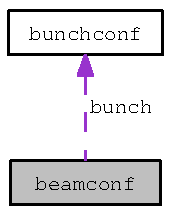
\includegraphics[width=59pt]{structbeamconf__coll__graph}
\end{center}
\end{figure}


\subsubsection{Detailed Description}
This structure contains the global beam parameters as well as a pointer to the array of bunches 

Definition at line 227 of file bpm\_\-interface.h.\subsubsection*{Data Fields}
\begin{CompactItemize}
\item 
int {\bf train\_\-num}
\item 
double {\bf beamrate}
\item 
double {\bf bunchrate}
\item 
int {\bf nbunches}
\item 
{\bf bunchconf\_\-t} $\ast$ {\bf bunch}
\item 
double {\bf position} [2]
\item 
double {\bf positionsigma} [2]
\item 
double {\bf slope} [2]
\item 
double {\bf slopesigma} [2]
\item 
double {\bf tilt} [2]
\item 
double {\bf tiltsigma} [2]
\item 
double {\bf bunchlength}
\item 
double {\bf bunchlengthsigma}
\item 
double {\bf energy}
\item 
double {\bf energysigma}
\item 
double {\bf charge}
\item 
double {\bf chargesigma}
\end{CompactItemize}


\subsubsection{Field Documentation}
\index{beamconf@{beamconf}!train\_\-num@{train\_\-num}}
\index{train\_\-num@{train\_\-num}!beamconf@{beamconf}}
\paragraph[train\_\-num]{\setlength{\rightskip}{0pt plus 5cm}int {\bf beamconf::train\_\-num}}\hfill\label{structbeamconf_f25a9f8d65fa4f04f9050414e0dcf891}


seq number of the train (evt num) 

Definition at line 228 of file bpm\_\-interface.h.\index{beamconf@{beamconf}!beamrate@{beamrate}}
\index{beamrate@{beamrate}!beamconf@{beamconf}}
\paragraph[beamrate]{\setlength{\rightskip}{0pt plus 5cm}double {\bf beamconf::beamrate}}\hfill\label{structbeamconf_9452259b166a06292909dd94e87bf9ae}


beam repetition rate (train to train) 

Definition at line 230 of file bpm\_\-interface.h.\index{beamconf@{beamconf}!bunchrate@{bunchrate}}
\index{bunchrate@{bunchrate}!beamconf@{beamconf}}
\paragraph[bunchrate]{\setlength{\rightskip}{0pt plus 5cm}double {\bf beamconf::bunchrate}}\hfill\label{structbeamconf_21abb80770607c1d48fef708c5dc4ebd}


bunch repetition rate (in the train) 

Definition at line 231 of file bpm\_\-interface.h.\index{beamconf@{beamconf}!nbunches@{nbunches}}
\index{nbunches@{nbunches}!beamconf@{beamconf}}
\paragraph[nbunches]{\setlength{\rightskip}{0pt plus 5cm}int {\bf beamconf::nbunches}}\hfill\label{structbeamconf_3957367666e4d2132d8a662941276f3a}


number of bunches per train 

Definition at line 232 of file bpm\_\-interface.h.

Referenced by generate\_\-bpmsignal(), and get\_\-bpmhits().\index{beamconf@{beamconf}!bunch@{bunch}}
\index{bunch@{bunch}!beamconf@{beamconf}}
\paragraph[bunch]{\setlength{\rightskip}{0pt plus 5cm}{\bf bunchconf\_\-t}$\ast$ {\bf beamconf::bunch}}\hfill\label{structbeamconf_9ded2879131ef6960f2c63893353c885}


list of pointers to the bunch conf structures 

Definition at line 234 of file bpm\_\-interface.h.

Referenced by generate\_\-bpmsignal(), and get\_\-bpmhits().\index{beamconf@{beamconf}!position@{position}}
\index{position@{position}!beamconf@{beamconf}}
\paragraph[position]{\setlength{\rightskip}{0pt plus 5cm}double {\bf beamconf::position}[2]}\hfill\label{structbeamconf_26b00990a201ad20363ff2affe6792fa}


beam position at the origin 

Definition at line 236 of file bpm\_\-interface.h.\index{beamconf@{beamconf}!positionsigma@{positionsigma}}
\index{positionsigma@{positionsigma}!beamconf@{beamconf}}
\paragraph[positionsigma]{\setlength{\rightskip}{0pt plus 5cm}double {\bf beamconf::positionsigma}[2]}\hfill\label{structbeamconf_3fd6fab4b89235e0a27d3733676f8eca}


position spread at the origin 

Definition at line 237 of file bpm\_\-interface.h.\index{beamconf@{beamconf}!slope@{slope}}
\index{slope@{slope}!beamconf@{beamconf}}
\paragraph[slope]{\setlength{\rightskip}{0pt plus 5cm}double {\bf beamconf::slope}[2]}\hfill\label{structbeamconf_71c30c68495a26878183645035cb8677}


beam slope at the origin 

Definition at line 239 of file bpm\_\-interface.h.\index{beamconf@{beamconf}!slopesigma@{slopesigma}}
\index{slopesigma@{slopesigma}!beamconf@{beamconf}}
\paragraph[slopesigma]{\setlength{\rightskip}{0pt plus 5cm}double {\bf beamconf::slopesigma}[2]}\hfill\label{structbeamconf_40ab197475399c5bb01b5abe25dee3d9}


slope spread at the origin 

Definition at line 240 of file bpm\_\-interface.h.\index{beamconf@{beamconf}!tilt@{tilt}}
\index{tilt@{tilt}!beamconf@{beamconf}}
\paragraph[tilt]{\setlength{\rightskip}{0pt plus 5cm}double {\bf beamconf::tilt}[2]}\hfill\label{structbeamconf_7465dd8acdcfce91e185a075334e2300}


bunch tilt at the origin 

Definition at line 242 of file bpm\_\-interface.h.\index{beamconf@{beamconf}!tiltsigma@{tiltsigma}}
\index{tiltsigma@{tiltsigma}!beamconf@{beamconf}}
\paragraph[tiltsigma]{\setlength{\rightskip}{0pt plus 5cm}double {\bf beamconf::tiltsigma}[2]}\hfill\label{structbeamconf_64040fb7876b2b4b8969154ab4aa387d}


tilt spread at the origin 

Definition at line 243 of file bpm\_\-interface.h.\index{beamconf@{beamconf}!bunchlength@{bunchlength}}
\index{bunchlength@{bunchlength}!beamconf@{beamconf}}
\paragraph[bunchlength]{\setlength{\rightskip}{0pt plus 5cm}double {\bf beamconf::bunchlength}}\hfill\label{structbeamconf_77503373031b8d15c31f697e8b8f5257}


bunch length at the origin 

Definition at line 245 of file bpm\_\-interface.h.\index{beamconf@{beamconf}!bunchlengthsigma@{bunchlengthsigma}}
\index{bunchlengthsigma@{bunchlengthsigma}!beamconf@{beamconf}}
\paragraph[bunchlengthsigma]{\setlength{\rightskip}{0pt plus 5cm}double {\bf beamconf::bunchlengthsigma}}\hfill\label{structbeamconf_166c8fdd8f3720c15faa4ba77b234d2c}


length spread at the origin 

Definition at line 246 of file bpm\_\-interface.h.\index{beamconf@{beamconf}!energy@{energy}}
\index{energy@{energy}!beamconf@{beamconf}}
\paragraph[energy]{\setlength{\rightskip}{0pt plus 5cm}double {\bf beamconf::energy}}\hfill\label{structbeamconf_259020346afa58ec8360e5098e8d9ab4}


beam energy (in GeV) at the origin 

Definition at line 248 of file bpm\_\-interface.h.\index{beamconf@{beamconf}!energysigma@{energysigma}}
\index{energysigma@{energysigma}!beamconf@{beamconf}}
\paragraph[energysigma]{\setlength{\rightskip}{0pt plus 5cm}double {\bf beamconf::energysigma}}\hfill\label{structbeamconf_3a7e535010155e32742b08a4a7b68415}


beam energy spread 

Definition at line 249 of file bpm\_\-interface.h.\index{beamconf@{beamconf}!charge@{charge}}
\index{charge@{charge}!beamconf@{beamconf}}
\paragraph[charge]{\setlength{\rightskip}{0pt plus 5cm}double {\bf beamconf::charge}}\hfill\label{structbeamconf_c06ea1a62a94875a08d0ff3ffeed5b18}


bunch charge (in nC) 

Definition at line 250 of file bpm\_\-interface.h.\index{beamconf@{beamconf}!chargesigma@{chargesigma}}
\index{chargesigma@{chargesigma}!beamconf@{beamconf}}
\paragraph[chargesigma]{\setlength{\rightskip}{0pt plus 5cm}double {\bf beamconf::chargesigma}}\hfill\label{structbeamconf_2bd344a9266ed88379a987c5a845f986}


charge spread 

Definition at line 251 of file bpm\_\-interface.h.

The documentation for this struct was generated from the following file:\begin{CompactItemize}
\item 
bpminterface/{\bf bpm\_\-interface.h}\end{CompactItemize}

\subsection{bpmcalib Struct Reference}
\label{structbpmcalib}\index{bpmcalib@{bpmcalib}}
{\tt \#include $<$bpm\_\-interface.h$>$}



\subsubsection{Detailed Description}
A structure containing the calibration information : purely calibration ! 

Definition at line 152 of file bpm\_\-interface.h.\subsubsection*{Data Fields}
\begin{CompactItemize}
\item 
double {\bf ddc\_\-IQphase}
\item 
double {\bf ddc\_\-posscale}
\item 
double {\bf ddc\_\-slopescale}
\item 
double {\bf ddc\_\-ct\_\-amp}
\item 
double {\bf ddc\_\-ct\_\-phase}
\item 
double {\bf fit\_\-IQphase}
\item 
double {\bf fit\_\-posscale}
\item 
double {\bf fit\_\-slopescale}
\item 
double {\bf fit\_\-ct\_\-amp}
\item 
double {\bf fit\_\-ct\_\-phase}
\end{CompactItemize}


\subsubsection{Field Documentation}
\index{bpmcalib@{bpmcalib}!ddc\_\-IQphase@{ddc\_\-IQphase}}
\index{ddc\_\-IQphase@{ddc\_\-IQphase}!bpmcalib@{bpmcalib}}
\paragraph[ddc\_\-IQphase]{\setlength{\rightskip}{0pt plus 5cm}double {\bf bpmcalib::ddc\_\-IQphase}}\hfill\label{structbpmcalib_2ea204a6c5a80f22b3edc99cf1f2100e}


processed IQ phase for the ddc routine 

Definition at line 154 of file bpm\_\-interface.h.

Referenced by postprocess\_\-waveform().\index{bpmcalib@{bpmcalib}!ddc\_\-posscale@{ddc\_\-posscale}}
\index{ddc\_\-posscale@{ddc\_\-posscale}!bpmcalib@{bpmcalib}}
\paragraph[ddc\_\-posscale]{\setlength{\rightskip}{0pt plus 5cm}double {\bf bpmcalib::ddc\_\-posscale}}\hfill\label{structbpmcalib_3ed4fc09eb4f328fe6f3013fe5d83efb}


processed position scale for the ddc routine 

Definition at line 155 of file bpm\_\-interface.h.

Referenced by postprocess\_\-waveform().\index{bpmcalib@{bpmcalib}!ddc\_\-slopescale@{ddc\_\-slopescale}}
\index{ddc\_\-slopescale@{ddc\_\-slopescale}!bpmcalib@{bpmcalib}}
\paragraph[ddc\_\-slopescale]{\setlength{\rightskip}{0pt plus 5cm}double {\bf bpmcalib::ddc\_\-slopescale}}\hfill\label{structbpmcalib_04bf942ef5b05de845c388ac355c5fa7}


processed slope scale for the fit routine 

Definition at line 156 of file bpm\_\-interface.h.

Referenced by postprocess\_\-waveform().\index{bpmcalib@{bpmcalib}!ddc\_\-ct\_\-amp@{ddc\_\-ct\_\-amp}}
\index{ddc\_\-ct\_\-amp@{ddc\_\-ct\_\-amp}!bpmcalib@{bpmcalib}}
\paragraph[ddc\_\-ct\_\-amp]{\setlength{\rightskip}{0pt plus 5cm}double {\bf bpmcalib::ddc\_\-ct\_\-amp}}\hfill\label{structbpmcalib_f5d9554311f52697ee793de6a14efb9c}


calibration tone amplitude at time of calibration 

Definition at line 157 of file bpm\_\-interface.h.

Referenced by correct\_\-gain().\index{bpmcalib@{bpmcalib}!ddc\_\-ct\_\-phase@{ddc\_\-ct\_\-phase}}
\index{ddc\_\-ct\_\-phase@{ddc\_\-ct\_\-phase}!bpmcalib@{bpmcalib}}
\paragraph[ddc\_\-ct\_\-phase]{\setlength{\rightskip}{0pt plus 5cm}double {\bf bpmcalib::ddc\_\-ct\_\-phase}}\hfill\label{structbpmcalib_2af30b1158dc11d6a7dba61e52b5d11c}


calibration tone phase at time of calibration 

Definition at line 158 of file bpm\_\-interface.h.

Referenced by correct\_\-gain().\index{bpmcalib@{bpmcalib}!fit\_\-IQphase@{fit\_\-IQphase}}
\index{fit\_\-IQphase@{fit\_\-IQphase}!bpmcalib@{bpmcalib}}
\paragraph[fit\_\-IQphase]{\setlength{\rightskip}{0pt plus 5cm}double {\bf bpmcalib::fit\_\-IQphase}}\hfill\label{structbpmcalib_de251f1e43e5d631283b36086916b5d8}


processed IQ phase for the fit routine 

Definition at line 161 of file bpm\_\-interface.h.

Referenced by postprocess\_\-waveform().\index{bpmcalib@{bpmcalib}!fit\_\-posscale@{fit\_\-posscale}}
\index{fit\_\-posscale@{fit\_\-posscale}!bpmcalib@{bpmcalib}}
\paragraph[fit\_\-posscale]{\setlength{\rightskip}{0pt plus 5cm}double {\bf bpmcalib::fit\_\-posscale}}\hfill\label{structbpmcalib_ce7dcc20bcfdf83fa642cf8ef5be273c}


position scale for the fit routine 

Definition at line 162 of file bpm\_\-interface.h.

Referenced by postprocess\_\-waveform().\index{bpmcalib@{bpmcalib}!fit\_\-slopescale@{fit\_\-slopescale}}
\index{fit\_\-slopescale@{fit\_\-slopescale}!bpmcalib@{bpmcalib}}
\paragraph[fit\_\-slopescale]{\setlength{\rightskip}{0pt plus 5cm}double {\bf bpmcalib::fit\_\-slopescale}}\hfill\label{structbpmcalib_8f4b5713433ab66b44a6f6a60ca7c64d}


slope scale for the fit routine 

Definition at line 163 of file bpm\_\-interface.h.

Referenced by postprocess\_\-waveform().\index{bpmcalib@{bpmcalib}!fit\_\-ct\_\-amp@{fit\_\-ct\_\-amp}}
\index{fit\_\-ct\_\-amp@{fit\_\-ct\_\-amp}!bpmcalib@{bpmcalib}}
\paragraph[fit\_\-ct\_\-amp]{\setlength{\rightskip}{0pt plus 5cm}double {\bf bpmcalib::fit\_\-ct\_\-amp}}\hfill\label{structbpmcalib_36b8871b5f00e1aadf0e78b0a2dca1ef}


calibration tone amplitude at time of calibration 

Definition at line 164 of file bpm\_\-interface.h.

Referenced by correct\_\-gain().\index{bpmcalib@{bpmcalib}!fit\_\-ct\_\-phase@{fit\_\-ct\_\-phase}}
\index{fit\_\-ct\_\-phase@{fit\_\-ct\_\-phase}!bpmcalib@{bpmcalib}}
\paragraph[fit\_\-ct\_\-phase]{\setlength{\rightskip}{0pt plus 5cm}double {\bf bpmcalib::fit\_\-ct\_\-phase}}\hfill\label{structbpmcalib_19628aa46fdec1c05e40b73df1d6f424}


calibration tone phase at time of calibration 

Definition at line 165 of file bpm\_\-interface.h.

Referenced by correct\_\-gain().

The documentation for this struct was generated from the following file:\begin{CompactItemize}
\item 
bpminterface/{\bf bpm\_\-interface.h}\end{CompactItemize}

\subsection{bpmconf Struct Reference}
\label{structbpmconf}\index{bpmconf@{bpmconf}}
{\tt \#include $<$bpm\_\-interface.h$>$}

Collaboration diagram for bpmconf:\nopagebreak
\begin{figure}[H]
\begin{center}
\leavevmode
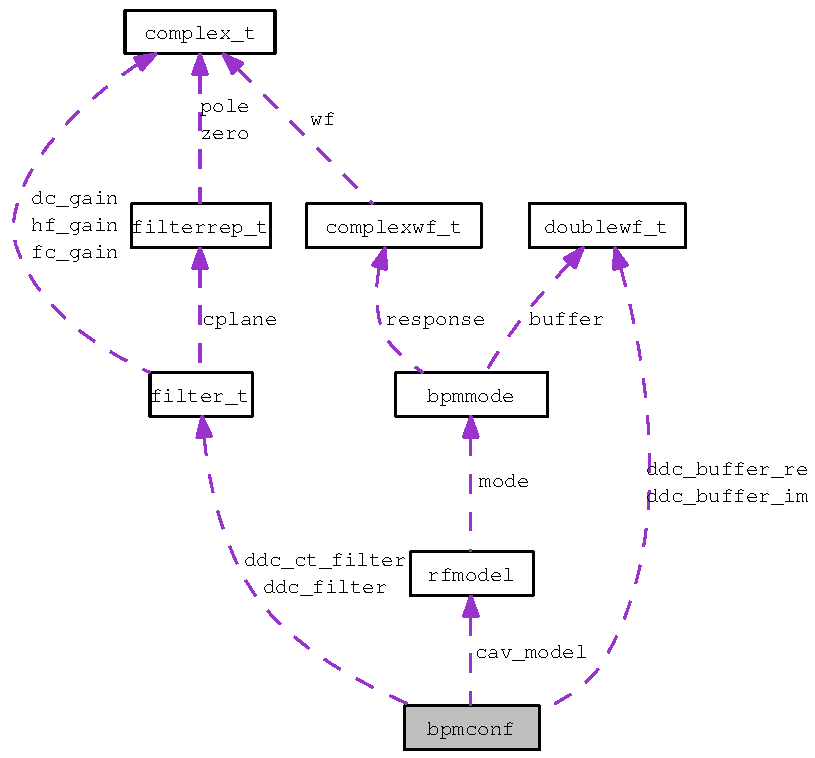
\includegraphics[width=400pt]{structbpmconf__coll__graph}
\end{center}
\end{figure}


\subsubsection{Detailed Description}
Structure containing the BPM configuration 

Definition at line 86 of file bpm\_\-interface.h.\subsubsection*{Data Fields}
\begin{CompactItemize}
\item 
char {\bf name} [20]
\item 
enum {\bf bpmtype\_\-t} {\bf cav\_\-type}
\item 
enum {\bf bpmpol\_\-t} {\bf cav\_\-polarisation}
\item 
enum {\bf bpmphase\_\-t} {\bf cav\_\-phasetype}
\item 
{\bf rfmodel\_\-t} $\ast$ \textbf{cav\_\-model}\label{structbpmconf_5a10e9ae753f6d357df5466d5c0f9b20}

\item 
double {\bf cav\_\-length}
\item 
double {\bf cav\_\-freq}
\item 
double {\bf cav\_\-decaytime}
\item 
double {\bf cav\_\-phase}
\item 
double {\bf cav\_\-iqrotation}
\item 
double {\bf cav\_\-chargesens}
\item 
double {\bf cav\_\-possens}
\item 
double {\bf cav\_\-tiltsens}
\item 
double {\bf rf\_\-LOfreq}
\item 
double {\bf digi\_\-trigtimeoffset}
\item 
double {\bf digi\_\-freq}
\item 
int {\bf digi\_\-nbits}
\item 
int {\bf digi\_\-nsamples}
\item 
double {\bf digi\_\-ampnoise}
\item 
int {\bf digi\_\-voltageoffset}
\item 
double {\bf digi\_\-phasenoise}
\item 
double {\bf t0}
\item 
double {\bf ddc\_\-freq}
\item 
double {\bf ddc\_\-tdecay}
\item 
double {\bf ddc\_\-tOffset}
\item 
{\bf filter\_\-t} $\ast$ {\bf ddc\_\-filter}
\item 
double {\bf fit\_\-inifreq}
\item 
double {\bf fit\_\-initdecay}
\item 
double {\bf fit\_\-tOffset}
\item 
double {\bf ddc\_\-ct\_\-freq}
\item 
{\bf filter\_\-t} $\ast$ {\bf ddc\_\-ct\_\-filter}
\item 
int {\bf ddc\_\-ct\_\-iSample}
\item 
double {\bf geom\_\-pos} [3]
\item 
double {\bf geom\_\-tilt} [3]
\item 
int {\bf ref\_\-idx}
\item 
int {\bf diode\_\-idx}
\item 
int {\bf forced\_\-trigger}
\item 
{\bf doublewf\_\-t} $\ast$ {\bf ddc\_\-buffer\_\-re}
\item 
{\bf doublewf\_\-t} $\ast$ {\bf ddc\_\-buffer\_\-im}
\end{CompactItemize}


\subsubsection{Field Documentation}
\index{bpmconf@{bpmconf}!name@{name}}
\index{name@{name}!bpmconf@{bpmconf}}
\paragraph[name]{\setlength{\rightskip}{0pt plus 5cm}char {\bf bpmconf::name}[20]}\hfill\label{structbpmconf_f9992502005d5a2a2af64bd71bb6d0e0}


a BPM should have a name 

Definition at line 87 of file bpm\_\-interface.h.

Referenced by postprocess\_\-waveform(), process\_\-caltone(), process\_\-diode(), process\_\-dipole(), process\_\-monopole(), and process\_\-waveform().\index{bpmconf@{bpmconf}!cav\_\-type@{cav\_\-type}}
\index{cav\_\-type@{cav\_\-type}!bpmconf@{bpmconf}}
\paragraph[cav\_\-type]{\setlength{\rightskip}{0pt plus 5cm}enum {\bf bpmtype\_\-t} {\bf bpmconf::cav\_\-type}}\hfill\label{structbpmconf_6360d70b5d4f4abfb37ca7e38df5b5ed}


BPM type 

Definition at line 89 of file bpm\_\-interface.h.

Referenced by process\_\-diode().\index{bpmconf@{bpmconf}!cav\_\-polarisation@{cav\_\-polarisation}}
\index{cav\_\-polarisation@{cav\_\-polarisation}!bpmconf@{bpmconf}}
\paragraph[cav\_\-polarisation]{\setlength{\rightskip}{0pt plus 5cm}enum {\bf bpmpol\_\-t} {\bf bpmconf::cav\_\-polarisation}}\hfill\label{structbpmconf_e7a0598eeb337a60a8c69d64c871e21b}


BPM polarisation 

Definition at line 90 of file bpm\_\-interface.h.\index{bpmconf@{bpmconf}!cav\_\-phasetype@{cav\_\-phasetype}}
\index{cav\_\-phasetype@{cav\_\-phasetype}!bpmconf@{bpmconf}}
\paragraph[cav\_\-phasetype]{\setlength{\rightskip}{0pt plus 5cm}enum {\bf bpmphase\_\-t} {\bf bpmconf::cav\_\-phasetype}}\hfill\label{structbpmconf_15efdd896d7cb61cc270f4fdb1d4a8b8}


BPM phase type 

Definition at line 91 of file bpm\_\-interface.h.\index{bpmconf@{bpmconf}!cav\_\-length@{cav\_\-length}}
\index{cav\_\-length@{cav\_\-length}!bpmconf@{bpmconf}}
\paragraph[cav\_\-length]{\setlength{\rightskip}{0pt plus 5cm}double {\bf bpmconf::cav\_\-length}}\hfill\label{structbpmconf_ab40b14a949f642e1bf125b0c1adbc46}


length of the cavity 

Definition at line 94 of file bpm\_\-interface.h.

Referenced by get\_\-mode\_\-amplitude().\index{bpmconf@{bpmconf}!cav\_\-freq@{cav\_\-freq}}
\index{cav\_\-freq@{cav\_\-freq}!bpmconf@{bpmconf}}
\paragraph[cav\_\-freq]{\setlength{\rightskip}{0pt plus 5cm}double {\bf bpmconf::cav\_\-freq}}\hfill\label{structbpmconf_0afced46dcedfaaf7f6bf5bccc54b3af}


cavity freq (MHz) 

Definition at line 95 of file bpm\_\-interface.h.\index{bpmconf@{bpmconf}!cav\_\-decaytime@{cav\_\-decaytime}}
\index{cav\_\-decaytime@{cav\_\-decaytime}!bpmconf@{bpmconf}}
\paragraph[cav\_\-decaytime]{\setlength{\rightskip}{0pt plus 5cm}double {\bf bpmconf::cav\_\-decaytime}}\hfill\label{structbpmconf_3a1e7d48a61675a0e40eb9a9eaddabcf}


cavity decay time (microsec) 

Definition at line 96 of file bpm\_\-interface.h.

Referenced by process\_\-waveform().\index{bpmconf@{bpmconf}!cav\_\-phase@{cav\_\-phase}}
\index{cav\_\-phase@{cav\_\-phase}!bpmconf@{bpmconf}}
\paragraph[cav\_\-phase]{\setlength{\rightskip}{0pt plus 5cm}double {\bf bpmconf::cav\_\-phase}}\hfill\label{structbpmconf_797ba2a47eb4568ffa42b211b7cfd919}


phase advance wrt. reference (fixed or random) 

Definition at line 97 of file bpm\_\-interface.h.\index{bpmconf@{bpmconf}!cav\_\-iqrotation@{cav\_\-iqrotation}}
\index{cav\_\-iqrotation@{cav\_\-iqrotation}!bpmconf@{bpmconf}}
\paragraph[cav\_\-iqrotation]{\setlength{\rightskip}{0pt plus 5cm}double {\bf bpmconf::cav\_\-iqrotation}}\hfill\label{structbpmconf_3f42d7001f93d0f5d96494fc56d34db4}


cavity IQ rotation 

Definition at line 98 of file bpm\_\-interface.h.\index{bpmconf@{bpmconf}!cav\_\-chargesens@{cav\_\-chargesens}}
\index{cav\_\-chargesens@{cav\_\-chargesens}!bpmconf@{bpmconf}}
\paragraph[cav\_\-chargesens]{\setlength{\rightskip}{0pt plus 5cm}double {\bf bpmconf::cav\_\-chargesens}}\hfill\label{structbpmconf_531fa3ac5f947a73104f2530d9201fe1}


charge sensitivity (volt/nC) 

Definition at line 99 of file bpm\_\-interface.h.\index{bpmconf@{bpmconf}!cav\_\-possens@{cav\_\-possens}}
\index{cav\_\-possens@{cav\_\-possens}!bpmconf@{bpmconf}}
\paragraph[cav\_\-possens]{\setlength{\rightskip}{0pt plus 5cm}double {\bf bpmconf::cav\_\-possens}}\hfill\label{structbpmconf_c71cb91910658b14805f0f2df775d800}


pos sensitivity at 1.6nC charge (volt/micron) 

Definition at line 100 of file bpm\_\-interface.h.\index{bpmconf@{bpmconf}!cav\_\-tiltsens@{cav\_\-tiltsens}}
\index{cav\_\-tiltsens@{cav\_\-tiltsens}!bpmconf@{bpmconf}}
\paragraph[cav\_\-tiltsens]{\setlength{\rightskip}{0pt plus 5cm}double {\bf bpmconf::cav\_\-tiltsens}}\hfill\label{structbpmconf_b36911235f88643648515d9e7221ba0a}


tilt sensitivity at 1.6nC charge (volt/micron) 

Definition at line 101 of file bpm\_\-interface.h.\index{bpmconf@{bpmconf}!rf\_\-LOfreq@{rf\_\-LOfreq}}
\index{rf\_\-LOfreq@{rf\_\-LOfreq}!bpmconf@{bpmconf}}
\paragraph[rf\_\-LOfreq]{\setlength{\rightskip}{0pt plus 5cm}double {\bf bpmconf::rf\_\-LOfreq}}\hfill\label{structbpmconf_93d6c265f81e710190e3def3e0e9f915}


LO frequency to mix down with (in MHz) 

Definition at line 103 of file bpm\_\-interface.h.\index{bpmconf@{bpmconf}!digi\_\-trigtimeoffset@{digi\_\-trigtimeoffset}}
\index{digi\_\-trigtimeoffset@{digi\_\-trigtimeoffset}!bpmconf@{bpmconf}}
\paragraph[digi\_\-trigtimeoffset]{\setlength{\rightskip}{0pt plus 5cm}double {\bf bpmconf::digi\_\-trigtimeoffset}}\hfill\label{structbpmconf_1a98df4d591675dde152fccb06e493e3}


time (usec) to offset bunch arrival times by 

Definition at line 106 of file bpm\_\-interface.h.\index{bpmconf@{bpmconf}!digi\_\-freq@{digi\_\-freq}}
\index{digi\_\-freq@{digi\_\-freq}!bpmconf@{bpmconf}}
\paragraph[digi\_\-freq]{\setlength{\rightskip}{0pt plus 5cm}double {\bf bpmconf::digi\_\-freq}}\hfill\label{structbpmconf_365b1e31d0d764deb0570b2aa1eede91}


digitization frequency (MHz) 

Definition at line 107 of file bpm\_\-interface.h.

Referenced by process\_\-waveform().\index{bpmconf@{bpmconf}!digi\_\-nbits@{digi\_\-nbits}}
\index{digi\_\-nbits@{digi\_\-nbits}!bpmconf@{bpmconf}}
\paragraph[digi\_\-nbits]{\setlength{\rightskip}{0pt plus 5cm}int {\bf bpmconf::digi\_\-nbits}}\hfill\label{structbpmconf_4590775f30535e00c5ec47c0f9c138ec}


number of bits in ADC for digitisation 

Definition at line 108 of file bpm\_\-interface.h.

Referenced by process\_\-caltone(), and process\_\-waveform().\index{bpmconf@{bpmconf}!digi\_\-nsamples@{digi\_\-nsamples}}
\index{digi\_\-nsamples@{digi\_\-nsamples}!bpmconf@{bpmconf}}
\paragraph[digi\_\-nsamples]{\setlength{\rightskip}{0pt plus 5cm}int {\bf bpmconf::digi\_\-nsamples}}\hfill\label{structbpmconf_fcbe4ae12ac60abee295c9261b9c4410}


number of samples in ADC digitisation 

Definition at line 109 of file bpm\_\-interface.h.

Referenced by process\_\-waveform().\index{bpmconf@{bpmconf}!digi\_\-ampnoise@{digi\_\-ampnoise}}
\index{digi\_\-ampnoise@{digi\_\-ampnoise}!bpmconf@{bpmconf}}
\paragraph[digi\_\-ampnoise]{\setlength{\rightskip}{0pt plus 5cm}double {\bf bpmconf::digi\_\-ampnoise}}\hfill\label{structbpmconf_08a2f1bf3b66aae4801db4e60b18e877}


amplitude noise in ADC channels (pedestal width) 

Definition at line 110 of file bpm\_\-interface.h.\index{bpmconf@{bpmconf}!digi\_\-voltageoffset@{digi\_\-voltageoffset}}
\index{digi\_\-voltageoffset@{digi\_\-voltageoffset}!bpmconf@{bpmconf}}
\paragraph[digi\_\-voltageoffset]{\setlength{\rightskip}{0pt plus 5cm}int {\bf bpmconf::digi\_\-voltageoffset}}\hfill\label{structbpmconf_9135fd99da4a801e88a66845a7c71ff9}


voltage offset (pedestal position) in counts 

Definition at line 111 of file bpm\_\-interface.h.\index{bpmconf@{bpmconf}!digi\_\-phasenoise@{digi\_\-phasenoise}}
\index{digi\_\-phasenoise@{digi\_\-phasenoise}!bpmconf@{bpmconf}}
\paragraph[digi\_\-phasenoise]{\setlength{\rightskip}{0pt plus 5cm}double {\bf bpmconf::digi\_\-phasenoise}}\hfill\label{structbpmconf_88562cd1feeaee818230b11035ef57a7}


phase noise 

Definition at line 112 of file bpm\_\-interface.h.\index{bpmconf@{bpmconf}!t0@{t0}}
\index{t0@{t0}!bpmconf@{bpmconf}}
\paragraph[t0]{\setlength{\rightskip}{0pt plus 5cm}double {\bf bpmconf::t0}}\hfill\label{structbpmconf_59157c2831c6191ccabfc702acddf02a}


start time of pulse 

Definition at line 116 of file bpm\_\-interface.h.

Referenced by process\_\-waveform().\index{bpmconf@{bpmconf}!ddc\_\-freq@{ddc\_\-freq}}
\index{ddc\_\-freq@{ddc\_\-freq}!bpmconf@{bpmconf}}
\paragraph[ddc\_\-freq]{\setlength{\rightskip}{0pt plus 5cm}double {\bf bpmconf::ddc\_\-freq}}\hfill\label{structbpmconf_6c054672fa971d58fd3c50040d9a7e57}


Frequency of downmixed waveform (MHz) 

Definition at line 119 of file bpm\_\-interface.h.

Referenced by process\_\-waveform().\index{bpmconf@{bpmconf}!ddc\_\-tdecay@{ddc\_\-tdecay}}
\index{ddc\_\-tdecay@{ddc\_\-tdecay}!bpmconf@{bpmconf}}
\paragraph[ddc\_\-tdecay]{\setlength{\rightskip}{0pt plus 5cm}double {\bf bpmconf::ddc\_\-tdecay}}\hfill\label{structbpmconf_626f42b1ed03ecc448dbf6a64852f793}


Decay time (usec) 

Definition at line 120 of file bpm\_\-interface.h.

Referenced by process\_\-waveform().\index{bpmconf@{bpmconf}!ddc\_\-tOffset@{ddc\_\-tOffset}}
\index{ddc\_\-tOffset@{ddc\_\-tOffset}!bpmconf@{bpmconf}}
\paragraph[ddc\_\-tOffset]{\setlength{\rightskip}{0pt plus 5cm}double {\bf bpmconf::ddc\_\-tOffset}}\hfill\label{structbpmconf_23a43814f2826696ea56587c81cdea4e}


Always have offset from t0 for sampling !!! 

Definition at line 121 of file bpm\_\-interface.h.

Referenced by process\_\-waveform().\index{bpmconf@{bpmconf}!ddc\_\-filter@{ddc\_\-filter}}
\index{ddc\_\-filter@{ddc\_\-filter}!bpmconf@{bpmconf}}
\paragraph[ddc\_\-filter]{\setlength{\rightskip}{0pt plus 5cm}{\bf filter\_\-t}$\ast$ {\bf bpmconf::ddc\_\-filter}}\hfill\label{structbpmconf_641616863daef1ba61c3962ee0f1feb3}


DDC 2 omega filter 

Definition at line 122 of file bpm\_\-interface.h.

Referenced by process\_\-waveform().\index{bpmconf@{bpmconf}!fit\_\-inifreq@{fit\_\-inifreq}}
\index{fit\_\-inifreq@{fit\_\-inifreq}!bpmconf@{bpmconf}}
\paragraph[fit\_\-inifreq]{\setlength{\rightskip}{0pt plus 5cm}double {\bf bpmconf::fit\_\-inifreq}}\hfill\label{structbpmconf_c874a126f597bef0e859829df40f6828}


Initial frequency for fitting 

Definition at line 125 of file bpm\_\-interface.h.\index{bpmconf@{bpmconf}!fit\_\-initdecay@{fit\_\-initdecay}}
\index{fit\_\-initdecay@{fit\_\-initdecay}!bpmconf@{bpmconf}}
\paragraph[fit\_\-initdecay]{\setlength{\rightskip}{0pt plus 5cm}double {\bf bpmconf::fit\_\-initdecay}}\hfill\label{structbpmconf_09649f2fb45b07b22a94841d28af91e7}


Initial decay time for fitting 

Definition at line 126 of file bpm\_\-interface.h.\index{bpmconf@{bpmconf}!fit\_\-tOffset@{fit\_\-tOffset}}
\index{fit\_\-tOffset@{fit\_\-tOffset}!bpmconf@{bpmconf}}
\paragraph[fit\_\-tOffset]{\setlength{\rightskip}{0pt plus 5cm}double {\bf bpmconf::fit\_\-tOffset}}\hfill\label{structbpmconf_10b19a4b942d4d29812197e3cd6614fe}


Offset from t0 to start fitting 

Definition at line 127 of file bpm\_\-interface.h.

Referenced by process\_\-waveform().\index{bpmconf@{bpmconf}!ddc\_\-ct\_\-freq@{ddc\_\-ct\_\-freq}}
\index{ddc\_\-ct\_\-freq@{ddc\_\-ct\_\-freq}!bpmconf@{bpmconf}}
\paragraph[ddc\_\-ct\_\-freq]{\setlength{\rightskip}{0pt plus 5cm}double {\bf bpmconf::ddc\_\-ct\_\-freq}}\hfill\label{structbpmconf_4161d0ffd2c54fa963cf647acee85d07}


caltone frequency for the ddc algorithm 

Definition at line 130 of file bpm\_\-interface.h.

Referenced by process\_\-caltone().\index{bpmconf@{bpmconf}!ddc\_\-ct\_\-filter@{ddc\_\-ct\_\-filter}}
\index{ddc\_\-ct\_\-filter@{ddc\_\-ct\_\-filter}!bpmconf@{bpmconf}}
\paragraph[ddc\_\-ct\_\-filter]{\setlength{\rightskip}{0pt plus 5cm}{\bf filter\_\-t}$\ast$ {\bf bpmconf::ddc\_\-ct\_\-filter}}\hfill\label{structbpmconf_c5f7ea44e1cbfa2b6efa35cb0fb3eb78}


filter for the caltone ddc 

Definition at line 131 of file bpm\_\-interface.h.

Referenced by process\_\-caltone().\index{bpmconf@{bpmconf}!ddc\_\-ct\_\-iSample@{ddc\_\-ct\_\-iSample}}
\index{ddc\_\-ct\_\-iSample@{ddc\_\-ct\_\-iSample}!bpmconf@{bpmconf}}
\paragraph[ddc\_\-ct\_\-iSample]{\setlength{\rightskip}{0pt plus 5cm}int {\bf bpmconf::ddc\_\-ct\_\-iSample}}\hfill\label{structbpmconf_22293d75805cdba7799374a11ec3efc7}


sample number to sample from ddc for amp/phase 

Definition at line 132 of file bpm\_\-interface.h.

Referenced by process\_\-caltone().\index{bpmconf@{bpmconf}!geom\_\-pos@{geom\_\-pos}}
\index{geom\_\-pos@{geom\_\-pos}!bpmconf@{bpmconf}}
\paragraph[geom\_\-pos]{\setlength{\rightskip}{0pt plus 5cm}double {\bf bpmconf::geom\_\-pos}[3]}\hfill\label{structbpmconf_c1d1faa7d508fc9c577426adb9a49e1f}


position of the BPM in the beamline 

Definition at line 136 of file bpm\_\-interface.h.

Referenced by get\_\-bpmhit().\index{bpmconf@{bpmconf}!geom\_\-tilt@{geom\_\-tilt}}
\index{geom\_\-tilt@{geom\_\-tilt}!bpmconf@{bpmconf}}
\paragraph[geom\_\-tilt]{\setlength{\rightskip}{0pt plus 5cm}double {\bf bpmconf::geom\_\-tilt}[3]}\hfill\label{structbpmconf_893d35f9c9c87b77f0314b8ed58928ee}


tilt of the BPM (0: xrot, 1: yrot, 2: zrot) 

Definition at line 137 of file bpm\_\-interface.h.

Referenced by get\_\-bpmhit().\index{bpmconf@{bpmconf}!ref\_\-idx@{ref\_\-idx}}
\index{ref\_\-idx@{ref\_\-idx}!bpmconf@{bpmconf}}
\paragraph[ref\_\-idx]{\setlength{\rightskip}{0pt plus 5cm}int {\bf bpmconf::ref\_\-idx}}\hfill\label{structbpmconf_d3858f7f6e82fd515a6f126b873a34f1}


reference cavity index for this BPM 

Definition at line 140 of file bpm\_\-interface.h.\index{bpmconf@{bpmconf}!diode\_\-idx@{diode\_\-idx}}
\index{diode\_\-idx@{diode\_\-idx}!bpmconf@{bpmconf}}
\paragraph[diode\_\-idx]{\setlength{\rightskip}{0pt plus 5cm}int {\bf bpmconf::diode\_\-idx}}\hfill\label{structbpmconf_d3877ddfdbd0ea0b459c01a9ad64e807}


reference diode index for this BPM 

Definition at line 141 of file bpm\_\-interface.h.\index{bpmconf@{bpmconf}!forced\_\-trigger@{forced\_\-trigger}}
\index{forced\_\-trigger@{forced\_\-trigger}!bpmconf@{bpmconf}}
\paragraph[forced\_\-trigger]{\setlength{\rightskip}{0pt plus 5cm}int {\bf bpmconf::forced\_\-trigger}}\hfill\label{structbpmconf_2a7324686323fe06ecbe81a6455e9d6f}


this cavity is abused as trigger signal 

Definition at line 142 of file bpm\_\-interface.h.

Referenced by process\_\-diode().\index{bpmconf@{bpmconf}!ddc\_\-buffer\_\-re@{ddc\_\-buffer\_\-re}}
\index{ddc\_\-buffer\_\-re@{ddc\_\-buffer\_\-re}!bpmconf@{bpmconf}}
\paragraph[ddc\_\-buffer\_\-re]{\setlength{\rightskip}{0pt plus 5cm}{\bf doublewf\_\-t}$\ast$ {\bf bpmconf::ddc\_\-buffer\_\-re}}\hfill\label{structbpmconf_b65d00543b88a7d2765d0a63419f4948}


pointer to a \doxyref{doublewf\_\-t}{p.}{structdoublewf__t} buffer 

Definition at line 145 of file bpm\_\-interface.h.

Referenced by process\_\-caltone(), and process\_\-waveform().\index{bpmconf@{bpmconf}!ddc\_\-buffer\_\-im@{ddc\_\-buffer\_\-im}}
\index{ddc\_\-buffer\_\-im@{ddc\_\-buffer\_\-im}!bpmconf@{bpmconf}}
\paragraph[ddc\_\-buffer\_\-im]{\setlength{\rightskip}{0pt plus 5cm}{\bf doublewf\_\-t}$\ast$ {\bf bpmconf::ddc\_\-buffer\_\-im}}\hfill\label{structbpmconf_6d4802e13e5838a5df80aeda01a1f5b2}


pointer to a \doxyref{doublewf\_\-t}{p.}{structdoublewf__t} buffer 

Definition at line 146 of file bpm\_\-interface.h.

Referenced by process\_\-caltone(), and process\_\-waveform().

The documentation for this struct was generated from the following file:\begin{CompactItemize}
\item 
bpminterface/{\bf bpm\_\-interface.h}\end{CompactItemize}

\subsection{bpmmode Struct Reference}
\label{structbpmmode}\index{bpmmode@{bpmmode}}
{\tt \#include $<$bpm\_\-interface.h$>$}

Collaboration diagram for bpmmode:\nopagebreak
\begin{figure}[H]
\begin{center}
\leavevmode
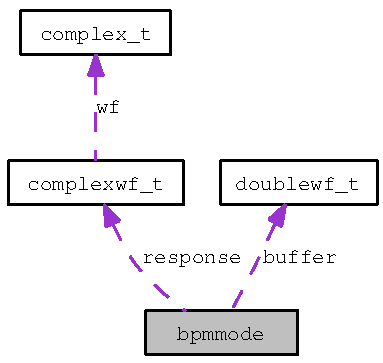
\includegraphics[width=110pt]{structbpmmode__coll__graph}
\end{center}
\end{figure}


\subsubsection{Detailed Description}
This structure defines a BPM resonant mode which is defined by it's resonant frequency, Q factor and sensitivities to the beam charge, slope and bunch tilt. 

Definition at line 282 of file bpm\_\-interface.h.\subsubsection*{Data Fields}
\begin{CompactItemize}
\item 
char {\bf name} [20]
\item 
double {\bf frequency}
\item 
double {\bf Q}
\item 
int {\bf order}
\item 
enum {\bf bpmpol\_\-t} {\bf polarisation}
\item 
double {\bf sensitivity}
\item 
{\bf complexwf\_\-t} $\ast$ {\bf response}
\item 
{\bf doublewf\_\-t} $\ast$ {\bf buffer}
\end{CompactItemize}


\subsubsection{Field Documentation}
\index{bpmmode@{bpmmode}!name@{name}}
\index{name@{name}!bpmmode@{bpmmode}}
\paragraph[name]{\setlength{\rightskip}{0pt plus 5cm}char {\bf bpmmode::name}[20]}\hfill\label{structbpmmode_8f3ec37ef0fdda0eeec8bf9a056f175a}


The name for the BPM mode, e.g \char`\"{}dipolex\char`\"{} 

Definition at line 283 of file bpm\_\-interface.h.

Referenced by generate\_\-bpmsignal().\index{bpmmode@{bpmmode}!frequency@{frequency}}
\index{frequency@{frequency}!bpmmode@{bpmmode}}
\paragraph[frequency]{\setlength{\rightskip}{0pt plus 5cm}double {\bf bpmmode::frequency}}\hfill\label{structbpmmode_b17dc935c70d7e9aec15d6ce93b14046}


The resonant frequency of the mode 

Definition at line 284 of file bpm\_\-interface.h.

Referenced by get\_\-mode\_\-amplitude(), and get\_\-mode\_\-response().\index{bpmmode@{bpmmode}!Q@{Q}}
\index{Q@{Q}!bpmmode@{bpmmode}}
\paragraph[Q]{\setlength{\rightskip}{0pt plus 5cm}double {\bf bpmmode::Q}}\hfill\label{structbpmmode_0d153f15610441366c0e2eb09089f092}


The Q factor for the mode 

Definition at line 285 of file bpm\_\-interface.h.

Referenced by get\_\-mode\_\-response().\index{bpmmode@{bpmmode}!order@{order}}
\index{order@{order}!bpmmode@{bpmmode}}
\paragraph[order]{\setlength{\rightskip}{0pt plus 5cm}int {\bf bpmmode::order}}\hfill\label{structbpmmode_90ab04d3b70f66e6a65e2399d92f018a}


The mode order, 0:monopole, 1:dipole, 2:quadrupole... 

Definition at line 286 of file bpm\_\-interface.h.

Referenced by add\_\-mode\_\-response(), get\_\-mode\_\-amplitude(), and get\_\-mode\_\-response().\index{bpmmode@{bpmmode}!polarisation@{polarisation}}
\index{polarisation@{polarisation}!bpmmode@{bpmmode}}
\paragraph[polarisation]{\setlength{\rightskip}{0pt plus 5cm}enum {\bf bpmpol\_\-t} {\bf bpmmode::polarisation}}\hfill\label{structbpmmode_72e607b92a918c1294d30523b39cff5b}


The mode polarisation: horiz, vert 

Definition at line 287 of file bpm\_\-interface.h.

Referenced by get\_\-mode\_\-amplitude().\index{bpmmode@{bpmmode}!sensitivity@{sensitivity}}
\index{sensitivity@{sensitivity}!bpmmode@{bpmmode}}
\paragraph[sensitivity]{\setlength{\rightskip}{0pt plus 5cm}double {\bf bpmmode::sensitivity}}\hfill\label{structbpmmode_9e0125d3567d1be32ce516fddf432e04}


The sensitivity of the mode, units depend on order 

Definition at line 288 of file bpm\_\-interface.h.

Referenced by get\_\-mode\_\-amplitude().\index{bpmmode@{bpmmode}!response@{response}}
\index{response@{response}!bpmmode@{bpmmode}}
\paragraph[response]{\setlength{\rightskip}{0pt plus 5cm}{\bf complexwf\_\-t}$\ast$ {\bf bpmmode::response}}\hfill\label{structbpmmode_52fbf2f821be6d800fc5937f38c0e04f}


Pointer to the mode response buffer 

Definition at line 289 of file bpm\_\-interface.h.

Referenced by add\_\-mode\_\-response(), generate\_\-bpmsignal(), and get\_\-mode\_\-response().\index{bpmmode@{bpmmode}!buffer@{buffer}}
\index{buffer@{buffer}!bpmmode@{bpmmode}}
\paragraph[buffer]{\setlength{\rightskip}{0pt plus 5cm}{\bf doublewf\_\-t}$\ast$ {\bf bpmmode::buffer}}\hfill\label{structbpmmode_64d7f14461813e77f2819be9b593cbcc}


Pointer to the mode's buffer 

Definition at line 290 of file bpm\_\-interface.h.

Referenced by generate\_\-bpmsignal().

The documentation for this struct was generated from the following file:\begin{CompactItemize}
\item 
bpminterface/{\bf bpm\_\-interface.h}\end{CompactItemize}

\subsection{bpmproc Struct Reference}
\label{structbpmproc}\index{bpmproc@{bpmproc}}
{\tt \#include $<$bpm\_\-interface.h$>$}

Collaboration diagram for bpmproc:\nopagebreak
\begin{figure}[H]
\begin{center}
\leavevmode
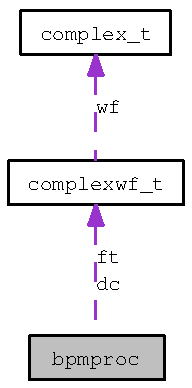
\includegraphics[width=64pt]{structbpmproc__coll__graph}
\end{center}
\end{figure}


\subsubsection{Detailed Description}
A structure containing the processed waveform information 

Definition at line 171 of file bpm\_\-interface.h.\subsubsection*{Data Fields}
\begin{CompactItemize}
\item 
double {\bf ampnoise}
\item 
double {\bf voltageoffset}
\item 
double {\bf t0}
\item 
int {\bf saturated}
\item 
int {\bf iunsat}
\item 
{\bf complexwf\_\-t} $\ast$ {\bf dc}
\item 
{\bf complexwf\_\-t} $\ast$ {\bf ft}
\item 
int {\bf fft\_\-success}
\item 
double {\bf fft\_\-amp}
\item 
double {\bf fft\_\-freq}
\item 
double {\bf fft\_\-tdecay}
\item 
double {\bf fft\_\-offset}
\item 
int {\bf ddc\_\-success}
\item 
double {\bf ddc\_\-tSample}
\item 
int {\bf ddc\_\-iSample}
\item 
double {\bf ddc\_\-Q}
\item 
double {\bf ddc\_\-I}
\item 
double {\bf ddc\_\-amp}
\item 
double {\bf ddc\_\-phase}
\item 
double {\bf ddc\_\-tdecay}
\item 
double {\bf ddc\_\-pos}
\item 
double {\bf ddc\_\-slope}
\item 
double {\bf ddc\_\-ct\_\-amp}
\item 
double {\bf ddc\_\-ct\_\-phase}
\item 
int {\bf fit\_\-success}
\item 
double {\bf fit\_\-Q}
\item 
double {\bf fit\_\-I}
\item 
double {\bf fit\_\-amp}
\item 
double {\bf fit\_\-phase}
\item 
double {\bf fit\_\-freq}
\item 
double {\bf fit\_\-tdecay}
\item 
double {\bf fit\_\-offset}
\item 
double {\bf fit\_\-pos}
\item 
double {\bf fit\_\-slope}
\item 
double {\bf fit\_\-ct\_\-amp}
\item 
double {\bf fit\_\-ct\_\-phase}
\end{CompactItemize}


\subsubsection{Field Documentation}
\index{bpmproc@{bpmproc}!ampnoise@{ampnoise}}
\index{ampnoise@{ampnoise}!bpmproc@{bpmproc}}
\paragraph[ampnoise]{\setlength{\rightskip}{0pt plus 5cm}double {\bf bpmproc::ampnoise}}\hfill\label{structbpmproc_03a2fb57c6fdaa5ea8558235bf69e5b2}


calculated (processed) amplitude noise 

Definition at line 172 of file bpm\_\-interface.h.

Referenced by process\_\-caltone(), and process\_\-waveform().\index{bpmproc@{bpmproc}!voltageoffset@{voltageoffset}}
\index{voltageoffset@{voltageoffset}!bpmproc@{bpmproc}}
\paragraph[voltageoffset]{\setlength{\rightskip}{0pt plus 5cm}double {\bf bpmproc::voltageoffset}}\hfill\label{structbpmproc_3be3f5398b06d6bb81f3fee29b6b904a}


calculated voltage offset 

Definition at line 173 of file bpm\_\-interface.h.

Referenced by process\_\-caltone(), and process\_\-waveform().\index{bpmproc@{bpmproc}!t0@{t0}}
\index{t0@{t0}!bpmproc@{bpmproc}}
\paragraph[t0]{\setlength{\rightskip}{0pt plus 5cm}double {\bf bpmproc::t0}}\hfill\label{structbpmproc_882cae0e540fd6d8557628a7edcb449d}


trigger t0 for int, copied from \doxyref{bpmconf\_\-t::t0}{p.}{structbpmconf_59157c2831c6191ccabfc702acddf02a} for ext 

Definition at line 175 of file bpm\_\-interface.h.

Referenced by process\_\-diode(), and process\_\-waveform().\index{bpmproc@{bpmproc}!saturated@{saturated}}
\index{saturated@{saturated}!bpmproc@{bpmproc}}
\paragraph[saturated]{\setlength{\rightskip}{0pt plus 5cm}int {\bf bpmproc::saturated}}\hfill\label{structbpmproc_611e04c6377faf4db9eb24a4edc1ac3f}


this signal was saturated 

Definition at line 177 of file bpm\_\-interface.h.

Referenced by process\_\-caltone(), and process\_\-waveform().\index{bpmproc@{bpmproc}!iunsat@{iunsat}}
\index{iunsat@{iunsat}!bpmproc@{bpmproc}}
\paragraph[iunsat]{\setlength{\rightskip}{0pt plus 5cm}int {\bf bpmproc::iunsat}}\hfill\label{structbpmproc_714ac2e4b3b26339aae97a0e5b32a300}


the last unsaturated sample index 

Definition at line 178 of file bpm\_\-interface.h.

Referenced by process\_\-caltone(), and process\_\-waveform().\index{bpmproc@{bpmproc}!dc@{dc}}
\index{dc@{dc}!bpmproc@{bpmproc}}
\paragraph[dc]{\setlength{\rightskip}{0pt plus 5cm}{\bf complexwf\_\-t}$\ast$ {\bf bpmproc::dc}}\hfill\label{structbpmproc_64c8db22258e28f24d7db38244b5df98}


The signal's DC waveform 

Definition at line 180 of file bpm\_\-interface.h.

Referenced by process\_\-caltone(), and process\_\-waveform().\index{bpmproc@{bpmproc}!ft@{ft}}
\index{ft@{ft}!bpmproc@{bpmproc}}
\paragraph[ft]{\setlength{\rightskip}{0pt plus 5cm}{\bf complexwf\_\-t}$\ast$ {\bf bpmproc::ft}}\hfill\label{structbpmproc_c6f3c265a080e664e10cc6f2339662a7}


The signal's fourier transform 

Definition at line 181 of file bpm\_\-interface.h.

Referenced by process\_\-caltone(), and process\_\-waveform().\index{bpmproc@{bpmproc}!fft\_\-success@{fft\_\-success}}
\index{fft\_\-success@{fft\_\-success}!bpmproc@{bpmproc}}
\paragraph[fft\_\-success]{\setlength{\rightskip}{0pt plus 5cm}int {\bf bpmproc::fft\_\-success}}\hfill\label{structbpmproc_cc0d36d5432742b3c68a7b3b4513e35e}


do we have proper fft info ? 

Definition at line 184 of file bpm\_\-interface.h.

Referenced by process\_\-caltone(), and process\_\-waveform().\index{bpmproc@{bpmproc}!fft\_\-amp@{fft\_\-amp}}
\index{fft\_\-amp@{fft\_\-amp}!bpmproc@{bpmproc}}
\paragraph[fft\_\-amp]{\setlength{\rightskip}{0pt plus 5cm}double {\bf bpmproc::fft\_\-amp}}\hfill\label{structbpmproc_31d52ab7354ff7176af4907efd51e4d0}


amplitude of fft 

Definition at line 185 of file bpm\_\-interface.h.\index{bpmproc@{bpmproc}!fft\_\-freq@{fft\_\-freq}}
\index{fft\_\-freq@{fft\_\-freq}!bpmproc@{bpmproc}}
\paragraph[fft\_\-freq]{\setlength{\rightskip}{0pt plus 5cm}double {\bf bpmproc::fft\_\-freq}}\hfill\label{structbpmproc_17d339f93b81bc99d632b9c5ffc8da85}


frequency obtained from fft (MHz) 

Definition at line 186 of file bpm\_\-interface.h.

Referenced by process\_\-caltone(), and process\_\-waveform().\index{bpmproc@{bpmproc}!fft\_\-tdecay@{fft\_\-tdecay}}
\index{fft\_\-tdecay@{fft\_\-tdecay}!bpmproc@{bpmproc}}
\paragraph[fft\_\-tdecay]{\setlength{\rightskip}{0pt plus 5cm}double {\bf bpmproc::fft\_\-tdecay}}\hfill\label{structbpmproc_ff324567b6af56170b2efe3f658eeac4}


decay time obtained from fft (usec) 

Definition at line 187 of file bpm\_\-interface.h.

Referenced by process\_\-caltone(), and process\_\-waveform().\index{bpmproc@{bpmproc}!fft\_\-offset@{fft\_\-offset}}
\index{fft\_\-offset@{fft\_\-offset}!bpmproc@{bpmproc}}
\paragraph[fft\_\-offset]{\setlength{\rightskip}{0pt plus 5cm}double {\bf bpmproc::fft\_\-offset}}\hfill\label{structbpmproc_6f8e0607ed73cdf3947ebfce7a876c79}


offset of fft in fit 

Definition at line 188 of file bpm\_\-interface.h.\index{bpmproc@{bpmproc}!ddc\_\-success@{ddc\_\-success}}
\index{ddc\_\-success@{ddc\_\-success}!bpmproc@{bpmproc}}
\paragraph[ddc\_\-success]{\setlength{\rightskip}{0pt plus 5cm}int {\bf bpmproc::ddc\_\-success}}\hfill\label{structbpmproc_7fdd95b16a37f79bec65bf7caaafe208}


do we have proper ddc info ? 

Definition at line 191 of file bpm\_\-interface.h.

Referenced by correct\_\-gain(), postprocess\_\-waveform(), process\_\-caltone(), and process\_\-waveform().\index{bpmproc@{bpmproc}!ddc\_\-tSample@{ddc\_\-tSample}}
\index{ddc\_\-tSample@{ddc\_\-tSample}!bpmproc@{bpmproc}}
\paragraph[ddc\_\-tSample]{\setlength{\rightskip}{0pt plus 5cm}double {\bf bpmproc::ddc\_\-tSample}}\hfill\label{structbpmproc_53c95ca0b2fa62c817fa4a14052f2a92}


time at which the ddc was sampled, t0+t0Offset 

Definition at line 192 of file bpm\_\-interface.h.

Referenced by process\_\-waveform().\index{bpmproc@{bpmproc}!ddc\_\-iSample@{ddc\_\-iSample}}
\index{ddc\_\-iSample@{ddc\_\-iSample}!bpmproc@{bpmproc}}
\paragraph[ddc\_\-iSample]{\setlength{\rightskip}{0pt plus 5cm}int {\bf bpmproc::ddc\_\-iSample}}\hfill\label{structbpmproc_c0632d46a0208577c352ea34bb69d983}


index of sample at which ddc sample was taken 

Definition at line 193 of file bpm\_\-interface.h.

Referenced by process\_\-waveform().\index{bpmproc@{bpmproc}!ddc\_\-Q@{ddc\_\-Q}}
\index{ddc\_\-Q@{ddc\_\-Q}!bpmproc@{bpmproc}}
\paragraph[ddc\_\-Q]{\setlength{\rightskip}{0pt plus 5cm}double {\bf bpmproc::ddc\_\-Q}}\hfill\label{structbpmproc_5c38241ca4aa400c93988106e8325d74}


ddc Q value 

Definition at line 194 of file bpm\_\-interface.h.

Referenced by postprocess\_\-waveform().\index{bpmproc@{bpmproc}!ddc\_\-I@{ddc\_\-I}}
\index{ddc\_\-I@{ddc\_\-I}!bpmproc@{bpmproc}}
\paragraph[ddc\_\-I]{\setlength{\rightskip}{0pt plus 5cm}double {\bf bpmproc::ddc\_\-I}}\hfill\label{structbpmproc_0f0ce52541c5965067e05669dbe96e5d}


ddc I value 

Definition at line 195 of file bpm\_\-interface.h.

Referenced by postprocess\_\-waveform().\index{bpmproc@{bpmproc}!ddc\_\-amp@{ddc\_\-amp}}
\index{ddc\_\-amp@{ddc\_\-amp}!bpmproc@{bpmproc}}
\paragraph[ddc\_\-amp]{\setlength{\rightskip}{0pt plus 5cm}double {\bf bpmproc::ddc\_\-amp}}\hfill\label{structbpmproc_f2defdec0144996a00deab9a30461241}


downconverted amplitude 

Definition at line 196 of file bpm\_\-interface.h.

Referenced by correct\_\-gain(), postprocess\_\-waveform(), process\_\-caltone(), and process\_\-waveform().\index{bpmproc@{bpmproc}!ddc\_\-phase@{ddc\_\-phase}}
\index{ddc\_\-phase@{ddc\_\-phase}!bpmproc@{bpmproc}}
\paragraph[ddc\_\-phase]{\setlength{\rightskip}{0pt plus 5cm}double {\bf bpmproc::ddc\_\-phase}}\hfill\label{structbpmproc_f2a86e422e93b453b91206abccc0b351}


downconverted phase 

Definition at line 197 of file bpm\_\-interface.h.

Referenced by correct\_\-gain(), postprocess\_\-waveform(), process\_\-caltone(), and process\_\-waveform().\index{bpmproc@{bpmproc}!ddc\_\-tdecay@{ddc\_\-tdecay}}
\index{ddc\_\-tdecay@{ddc\_\-tdecay}!bpmproc@{bpmproc}}
\paragraph[ddc\_\-tdecay]{\setlength{\rightskip}{0pt plus 5cm}double {\bf bpmproc::ddc\_\-tdecay}}\hfill\label{structbpmproc_0995020ee3f75e51ec9e07c054da14c2}


downconverted decay time of waveform 

Definition at line 198 of file bpm\_\-interface.h.\index{bpmproc@{bpmproc}!ddc\_\-pos@{ddc\_\-pos}}
\index{ddc\_\-pos@{ddc\_\-pos}!bpmproc@{bpmproc}}
\paragraph[ddc\_\-pos]{\setlength{\rightskip}{0pt plus 5cm}double {\bf bpmproc::ddc\_\-pos}}\hfill\label{structbpmproc_854f812a0660f45b42785180575f03af}


calculated position from ddc 

Definition at line 200 of file bpm\_\-interface.h.

Referenced by ana\_\-compute\_\-residual(), and postprocess\_\-waveform().\index{bpmproc@{bpmproc}!ddc\_\-slope@{ddc\_\-slope}}
\index{ddc\_\-slope@{ddc\_\-slope}!bpmproc@{bpmproc}}
\paragraph[ddc\_\-slope]{\setlength{\rightskip}{0pt plus 5cm}double {\bf bpmproc::ddc\_\-slope}}\hfill\label{structbpmproc_77e55611d4500f3be3d9c3d0437cf033}


calculated slope from ddc 

Definition at line 201 of file bpm\_\-interface.h.

Referenced by ana\_\-compute\_\-residual(), and postprocess\_\-waveform().\index{bpmproc@{bpmproc}!ddc\_\-ct\_\-amp@{ddc\_\-ct\_\-amp}}
\index{ddc\_\-ct\_\-amp@{ddc\_\-ct\_\-amp}!bpmproc@{bpmproc}}
\paragraph[ddc\_\-ct\_\-amp]{\setlength{\rightskip}{0pt plus 5cm}double {\bf bpmproc::ddc\_\-ct\_\-amp}}\hfill\label{structbpmproc_e3b787a2ed21acdf52ad9b667f57976e}


last measured calibration tone amplitude for this bpm 

Definition at line 203 of file bpm\_\-interface.h.

Referenced by correct\_\-gain(), and process\_\-caltone().\index{bpmproc@{bpmproc}!ddc\_\-ct\_\-phase@{ddc\_\-ct\_\-phase}}
\index{ddc\_\-ct\_\-phase@{ddc\_\-ct\_\-phase}!bpmproc@{bpmproc}}
\paragraph[ddc\_\-ct\_\-phase]{\setlength{\rightskip}{0pt plus 5cm}double {\bf bpmproc::ddc\_\-ct\_\-phase}}\hfill\label{structbpmproc_5461033608c7c42d900d25b7ead44153}


last measured calibration tone phase for this bpm 

Definition at line 204 of file bpm\_\-interface.h.

Referenced by correct\_\-gain(), and process\_\-caltone().\index{bpmproc@{bpmproc}!fit\_\-success@{fit\_\-success}}
\index{fit\_\-success@{fit\_\-success}!bpmproc@{bpmproc}}
\paragraph[fit\_\-success]{\setlength{\rightskip}{0pt plus 5cm}int {\bf bpmproc::fit\_\-success}}\hfill\label{structbpmproc_bcca38f653578b267a8b378c0bf22dee}


do we have proper fit info ? 

Definition at line 207 of file bpm\_\-interface.h.

Referenced by correct\_\-gain(), postprocess\_\-waveform(), and process\_\-waveform().\index{bpmproc@{bpmproc}!fit\_\-Q@{fit\_\-Q}}
\index{fit\_\-Q@{fit\_\-Q}!bpmproc@{bpmproc}}
\paragraph[fit\_\-Q]{\setlength{\rightskip}{0pt plus 5cm}double {\bf bpmproc::fit\_\-Q}}\hfill\label{structbpmproc_ad1d52ffea6d3a39b6e0d672c693ae36}


fit Q value 

Definition at line 208 of file bpm\_\-interface.h.

Referenced by postprocess\_\-waveform().\index{bpmproc@{bpmproc}!fit\_\-I@{fit\_\-I}}
\index{fit\_\-I@{fit\_\-I}!bpmproc@{bpmproc}}
\paragraph[fit\_\-I]{\setlength{\rightskip}{0pt plus 5cm}double {\bf bpmproc::fit\_\-I}}\hfill\label{structbpmproc_59924e30e71461ad0a2146a0be873bdf}


fit I value 

Definition at line 209 of file bpm\_\-interface.h.

Referenced by postprocess\_\-waveform().\index{bpmproc@{bpmproc}!fit\_\-amp@{fit\_\-amp}}
\index{fit\_\-amp@{fit\_\-amp}!bpmproc@{bpmproc}}
\paragraph[fit\_\-amp]{\setlength{\rightskip}{0pt plus 5cm}double {\bf bpmproc::fit\_\-amp}}\hfill\label{structbpmproc_ad6477fbcd2c2ead538bef6e17c27022}


fitted amplitude 

Definition at line 210 of file bpm\_\-interface.h.

Referenced by correct\_\-gain(), postprocess\_\-waveform(), and process\_\-waveform().\index{bpmproc@{bpmproc}!fit\_\-phase@{fit\_\-phase}}
\index{fit\_\-phase@{fit\_\-phase}!bpmproc@{bpmproc}}
\paragraph[fit\_\-phase]{\setlength{\rightskip}{0pt plus 5cm}double {\bf bpmproc::fit\_\-phase}}\hfill\label{structbpmproc_eb36a2ab357ca13c3c8352feb8cb6e8d}


fitted phase 

Definition at line 211 of file bpm\_\-interface.h.

Referenced by correct\_\-gain(), postprocess\_\-waveform(), and process\_\-waveform().\index{bpmproc@{bpmproc}!fit\_\-freq@{fit\_\-freq}}
\index{fit\_\-freq@{fit\_\-freq}!bpmproc@{bpmproc}}
\paragraph[fit\_\-freq]{\setlength{\rightskip}{0pt plus 5cm}double {\bf bpmproc::fit\_\-freq}}\hfill\label{structbpmproc_95c3ffbd8041ee333f7fb197b80d79b3}


fitted frequency (MHz) 

Definition at line 212 of file bpm\_\-interface.h.

Referenced by process\_\-waveform().\index{bpmproc@{bpmproc}!fit\_\-tdecay@{fit\_\-tdecay}}
\index{fit\_\-tdecay@{fit\_\-tdecay}!bpmproc@{bpmproc}}
\paragraph[fit\_\-tdecay]{\setlength{\rightskip}{0pt plus 5cm}double {\bf bpmproc::fit\_\-tdecay}}\hfill\label{structbpmproc_7f14eec6bdb4338ddc1f25b7f83d6c27}


fitted decay time of waveform (usec) 

Definition at line 213 of file bpm\_\-interface.h.

Referenced by process\_\-waveform().\index{bpmproc@{bpmproc}!fit\_\-offset@{fit\_\-offset}}
\index{fit\_\-offset@{fit\_\-offset}!bpmproc@{bpmproc}}
\paragraph[fit\_\-offset]{\setlength{\rightskip}{0pt plus 5cm}double {\bf bpmproc::fit\_\-offset}}\hfill\label{structbpmproc_b63c916c7ecdc62e9b39485892129d90}


fitted offset for waveform 

Definition at line 214 of file bpm\_\-interface.h.\index{bpmproc@{bpmproc}!fit\_\-pos@{fit\_\-pos}}
\index{fit\_\-pos@{fit\_\-pos}!bpmproc@{bpmproc}}
\paragraph[fit\_\-pos]{\setlength{\rightskip}{0pt plus 5cm}double {\bf bpmproc::fit\_\-pos}}\hfill\label{structbpmproc_96e0fb7e2c1ca6d244d3becd82a4aead}


calculated position from fit 

Definition at line 216 of file bpm\_\-interface.h.

Referenced by postprocess\_\-waveform().\index{bpmproc@{bpmproc}!fit\_\-slope@{fit\_\-slope}}
\index{fit\_\-slope@{fit\_\-slope}!bpmproc@{bpmproc}}
\paragraph[fit\_\-slope]{\setlength{\rightskip}{0pt plus 5cm}double {\bf bpmproc::fit\_\-slope}}\hfill\label{structbpmproc_735a81b589d083cfa4f5c172577774a1}


calculated slope from fit 

Definition at line 217 of file bpm\_\-interface.h.

Referenced by postprocess\_\-waveform().\index{bpmproc@{bpmproc}!fit\_\-ct\_\-amp@{fit\_\-ct\_\-amp}}
\index{fit\_\-ct\_\-amp@{fit\_\-ct\_\-amp}!bpmproc@{bpmproc}}
\paragraph[fit\_\-ct\_\-amp]{\setlength{\rightskip}{0pt plus 5cm}double {\bf bpmproc::fit\_\-ct\_\-amp}}\hfill\label{structbpmproc_642c32e284ca90dc6f0f13a8a0e60176}


last measured calibration tone amplitude for this bpm 

Definition at line 219 of file bpm\_\-interface.h.

Referenced by correct\_\-gain().\index{bpmproc@{bpmproc}!fit\_\-ct\_\-phase@{fit\_\-ct\_\-phase}}
\index{fit\_\-ct\_\-phase@{fit\_\-ct\_\-phase}!bpmproc@{bpmproc}}
\paragraph[fit\_\-ct\_\-phase]{\setlength{\rightskip}{0pt plus 5cm}double {\bf bpmproc::fit\_\-ct\_\-phase}}\hfill\label{structbpmproc_047ed884dc6bc77d4829d83176943ef1}


last measured calibration tone phase for this bpm 

Definition at line 220 of file bpm\_\-interface.h.

Referenced by correct\_\-gain().

The documentation for this struct was generated from the following file:\begin{CompactItemize}
\item 
bpminterface/{\bf bpm\_\-interface.h}\end{CompactItemize}

\subsection{bunchconf Struct Reference}
\label{structbunchconf}\index{bunchconf@{bunchconf}}
{\tt \#include $<$bpm\_\-interface.h$>$}



\subsubsection{Detailed Description}
This structure contains information on a single bunch inside the bunchtrain, which has its own energy, internal energy spread, charge, length, position/slope/tilt in the world coo frame and position/slope/tilt in the BPM local coo frame. 

Definition at line 260 of file bpm\_\-interface.h.\subsubsection*{Data Fields}
\begin{CompactItemize}
\item 
int {\bf train\_\-num}
\item 
int {\bf bunch\_\-num}
\item 
double {\bf energy}
\item 
double {\bf energyspread}
\item 
double \textbf{charge}\label{structbunchconf_2d39addc39dc701e488faaace1d7b711}

\item 
double {\bf length}
\item 
double {\bf arrival\_\-time}
\item 
double {\bf position} [2]
\item 
double {\bf slope} [2]
\item 
double {\bf tilt} [2]
\item 
double {\bf bpmposition} [3]
\item 
double {\bf bpmslope} [2]
\item 
double {\bf bpmtilt} [2]
\end{CompactItemize}


\subsubsection{Field Documentation}
\index{bunchconf@{bunchconf}!train\_\-num@{train\_\-num}}
\index{train\_\-num@{train\_\-num}!bunchconf@{bunchconf}}
\paragraph[train\_\-num]{\setlength{\rightskip}{0pt plus 5cm}int {\bf bunchconf::train\_\-num}}\hfill\label{structbunchconf_bf9be3f4dbb15b1dd2392265f7ce0b83}


seq number of the train this bunch belongs to 

Definition at line 261 of file bpm\_\-interface.h.\index{bunchconf@{bunchconf}!bunch\_\-num@{bunch\_\-num}}
\index{bunch\_\-num@{bunch\_\-num}!bunchconf@{bunchconf}}
\paragraph[bunch\_\-num]{\setlength{\rightskip}{0pt plus 5cm}int {\bf bunchconf::bunch\_\-num}}\hfill\label{structbunchconf_eb875731eeb9ed42e0ff30356bbf77d2}


seq number of the bunch in the train 

Definition at line 262 of file bpm\_\-interface.h.\index{bunchconf@{bunchconf}!energy@{energy}}
\index{energy@{energy}!bunchconf@{bunchconf}}
\paragraph[energy]{\setlength{\rightskip}{0pt plus 5cm}double {\bf bunchconf::energy}}\hfill\label{structbunchconf_4b460ca05a551c27b1971d0d9f9cd448}


energy of the bunch 

Definition at line 264 of file bpm\_\-interface.h.\index{bunchconf@{bunchconf}!energyspread@{energyspread}}
\index{energyspread@{energyspread}!bunchconf@{bunchconf}}
\paragraph[energyspread]{\setlength{\rightskip}{0pt plus 5cm}double {\bf bunchconf::energyspread}}\hfill\label{structbunchconf_3025ff841f30742837034239fa94cee8}


energy spread inside the bunch 

Definition at line 265 of file bpm\_\-interface.h.\index{bunchconf@{bunchconf}!length@{length}}
\index{length@{length}!bunchconf@{bunchconf}}
\paragraph[length]{\setlength{\rightskip}{0pt plus 5cm}double {\bf bunchconf::length}}\hfill\label{structbunchconf_d0f7556a5e2d780a9925377b5decda90}


the bunch length 

Definition at line 267 of file bpm\_\-interface.h.

Referenced by get\_\-mode\_\-amplitude().\index{bunchconf@{bunchconf}!arrival\_\-time@{arrival\_\-time}}
\index{arrival\_\-time@{arrival\_\-time}!bunchconf@{bunchconf}}
\paragraph[arrival\_\-time]{\setlength{\rightskip}{0pt plus 5cm}double {\bf bunchconf::arrival\_\-time}}\hfill\label{structbunchconf_e2cb9e35f4ee18761393b29ef6e0de9a}


arrival time of bunch 

Definition at line 268 of file bpm\_\-interface.h.

Referenced by generate\_\-bpmsignal().\index{bunchconf@{bunchconf}!position@{position}}
\index{position@{position}!bunchconf@{bunchconf}}
\paragraph[position]{\setlength{\rightskip}{0pt plus 5cm}double {\bf bunchconf::position}[2]}\hfill\label{structbunchconf_d2f81b99a529249ff6cfdb85886d3f07}


the bunch position x,y at the bpm coo 

Definition at line 269 of file bpm\_\-interface.h.

Referenced by get\_\-bpmhit().\index{bunchconf@{bunchconf}!slope@{slope}}
\index{slope@{slope}!bunchconf@{bunchconf}}
\paragraph[slope]{\setlength{\rightskip}{0pt plus 5cm}double {\bf bunchconf::slope}[2]}\hfill\label{structbunchconf_867a15a56a3a60db2360b8645756cb71}


the bunch slope x',y' at the bpm coo 

Definition at line 270 of file bpm\_\-interface.h.

Referenced by get\_\-bpmhit().\index{bunchconf@{bunchconf}!tilt@{tilt}}
\index{tilt@{tilt}!bunchconf@{bunchconf}}
\paragraph[tilt]{\setlength{\rightskip}{0pt plus 5cm}double {\bf bunchconf::tilt}[2]}\hfill\label{structbunchconf_ed8955a77ae6a4147f4877dfd413c4b7}


the bunch tilt x',y' at the bpm coo 

Definition at line 271 of file bpm\_\-interface.h.\index{bunchconf@{bunchconf}!bpmposition@{bpmposition}}
\index{bpmposition@{bpmposition}!bunchconf@{bunchconf}}
\paragraph[bpmposition]{\setlength{\rightskip}{0pt plus 5cm}double {\bf bunchconf::bpmposition}[3]}\hfill\label{structbunchconf_09345bb14a68c2391548054aa3cc5143}


where the beam hits the BPM in the BPM local co 

Definition at line 273 of file bpm\_\-interface.h.

Referenced by get\_\-bpmhit(), get\_\-mode\_\-amplitude(), and setup\_\-calibration().\index{bunchconf@{bunchconf}!bpmslope@{bpmslope}}
\index{bpmslope@{bpmslope}!bunchconf@{bunchconf}}
\paragraph[bpmslope]{\setlength{\rightskip}{0pt plus 5cm}double {\bf bunchconf::bpmslope}[2]}\hfill\label{structbunchconf_97cf9b9382c9b00b163ec51f00593bf1}


slope of beam through the BPM in BPM local co 

Definition at line 274 of file bpm\_\-interface.h.

Referenced by get\_\-bpmhit(), and get\_\-mode\_\-amplitude().\index{bunchconf@{bunchconf}!bpmtilt@{bpmtilt}}
\index{bpmtilt@{bpmtilt}!bunchconf@{bunchconf}}
\paragraph[bpmtilt]{\setlength{\rightskip}{0pt plus 5cm}double {\bf bunchconf::bpmtilt}[2]}\hfill\label{structbunchconf_02a745532d1169ab016f2c6ded81938c}


bunch tilt in the BPM local co 

Definition at line 275 of file bpm\_\-interface.h.

Referenced by get\_\-bpmhit().

The documentation for this struct was generated from the following file:\begin{CompactItemize}
\item 
bpminterface/{\bf bpm\_\-interface.h}\end{CompactItemize}

\subsection{complex\_\-t Struct Reference}
\label{structcomplex__t}\index{complex\_\-t@{complex\_\-t}}
{\tt \#include $<$bpm\_\-nr.h$>$}



\subsubsection{Detailed Description}
Structure and typedef for complex numbers used in the bpmdsp module 

Definition at line 206 of file bpm\_\-nr.h.\subsubsection*{Data Fields}
\begin{CompactItemize}
\item 
double \textbf{re}\label{structcomplex__t_ec1e67233fb6806c75b83af9bb83ff77}

\item 
double \textbf{im}\label{structcomplex__t_0a5273e242bd318097898ba9bb2bd625}

\end{CompactItemize}


The documentation for this struct was generated from the following file:\begin{CompactItemize}
\item 
bpmnr/{\bf bpm\_\-nr.h}\end{CompactItemize}

\subsection{complexwf\_\-t Struct Reference}
\label{structcomplexwf__t}\index{complexwf\_\-t@{complexwf\_\-t}}
{\tt \#include $<$bpm\_\-wf.h$>$}

Collaboration diagram for complexwf\_\-t:\nopagebreak
\begin{figure}[H]
\begin{center}
\leavevmode
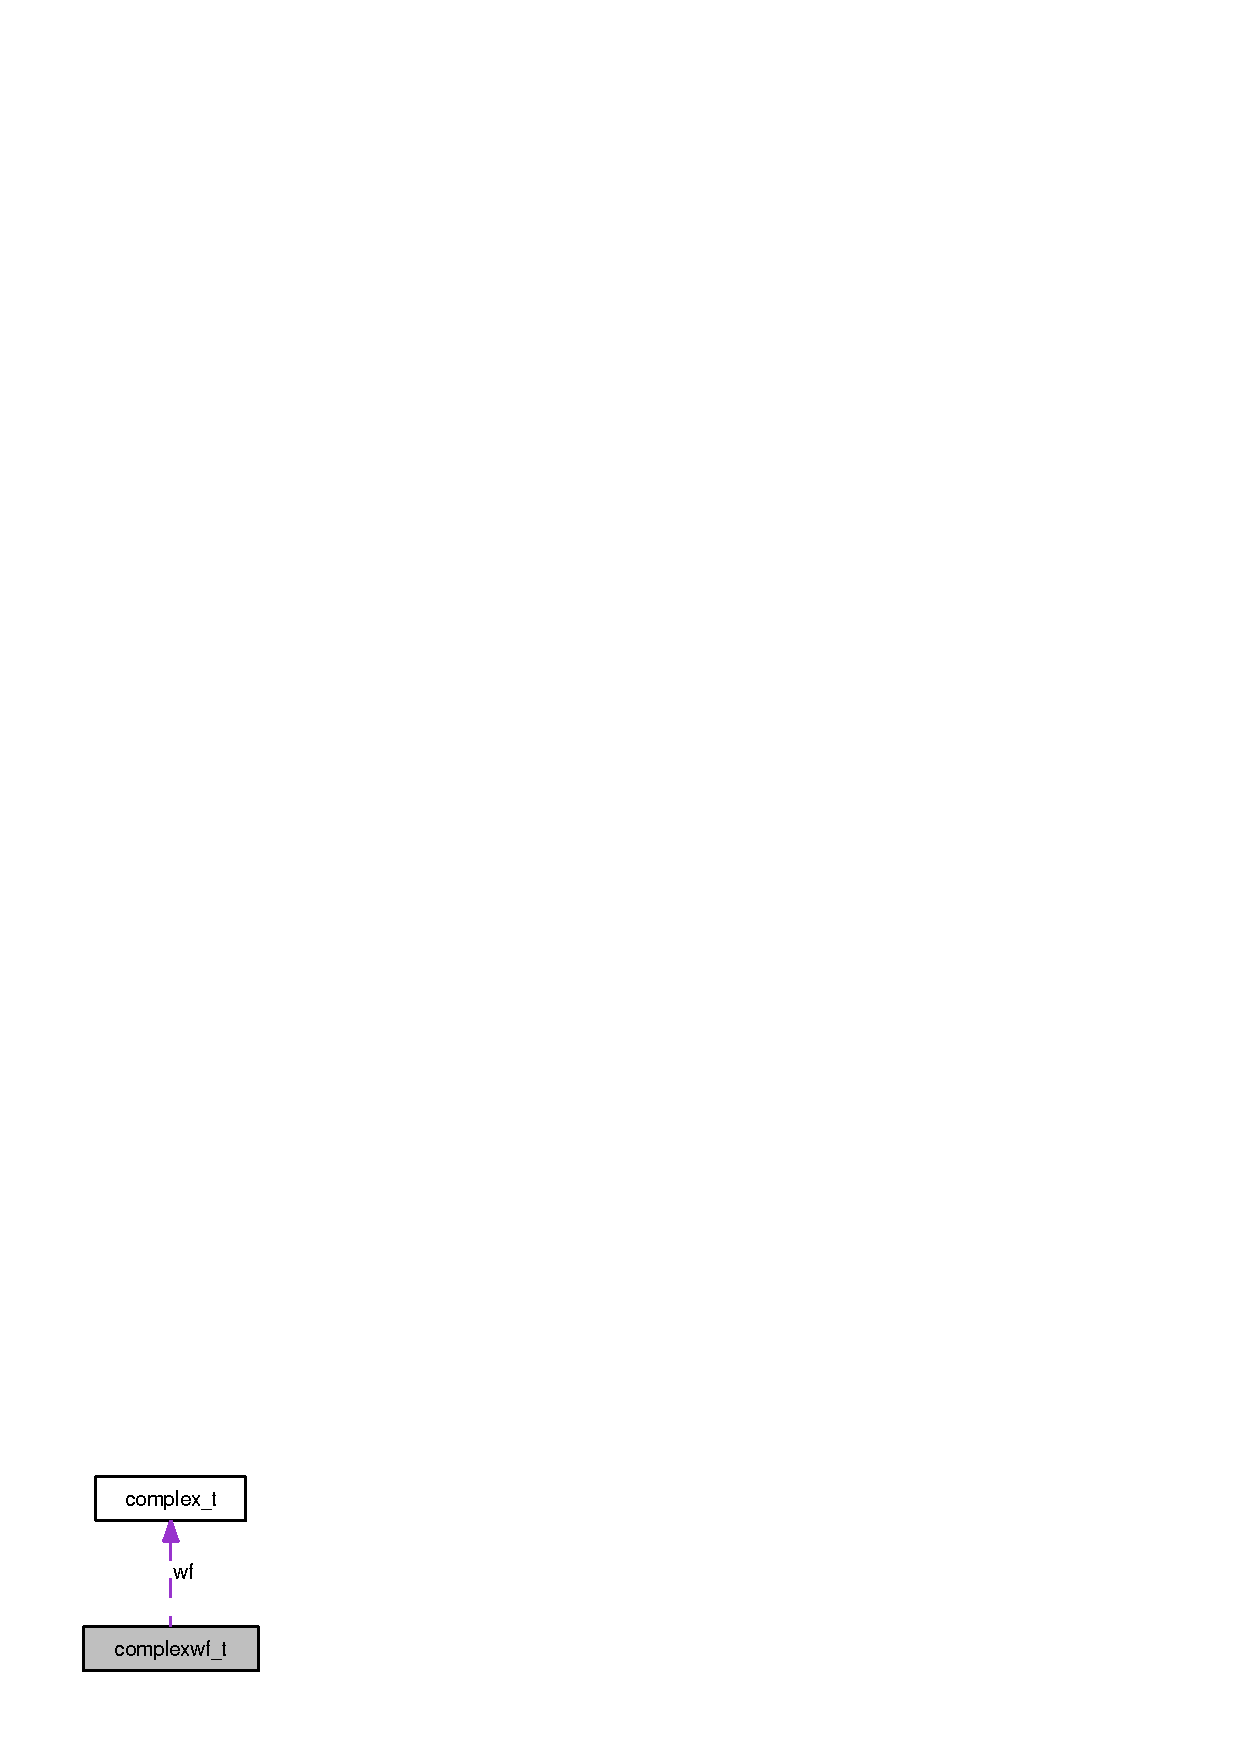
\includegraphics[width=64pt]{structcomplexwf__t__coll__graph}
\end{center}
\end{figure}


\subsubsection{Detailed Description}
Structure representing a waveform of complex numbers 

Definition at line 188 of file bpm\_\-wf.h.\subsubsection*{Data Fields}
\begin{CompactItemize}
\item 
int {\bf ns}
\item 
double {\bf fs}
\item 
{\bf complex\_\-t} $\ast$ {\bf wf}
\end{CompactItemize}


\subsubsection{Field Documentation}
\index{complexwf\_\-t@{complexwf\_\-t}!ns@{ns}}
\index{ns@{ns}!complexwf_t@{complexwf\_\-t}}
\paragraph[ns]{\setlength{\rightskip}{0pt plus 5cm}int {\bf complexwf\_\-t::ns}}\hfill\label{structcomplexwf__t_6ca8e343a776b345f6753539f2c2d865}


The number of samples in the waveform 

Definition at line 189 of file bpm\_\-wf.h.

Referenced by add\_\-mode\_\-response(), complexfft(), complexwf(), complexwf\_\-add(), complexwf\_\-add\_\-ampnoise(), complexwf\_\-add\_\-cwtone(), complexwf\_\-add\_\-dcywave(), complexwf\_\-add\_\-noise(), complexwf\_\-add\_\-phasenoise(), complexwf\_\-bias(), complexwf\_\-compat(), complexwf\_\-copy(), complexwf\_\-copy\_\-new(), complexwf\_\-divide(), complexwf\_\-getamp(), complexwf\_\-getamp\_\-new(), complexwf\_\-getimag(), complexwf\_\-getimag\_\-new(), complexwf\_\-getphase(), complexwf\_\-getphase\_\-new(), complexwf\_\-getreal(), complexwf\_\-getreal\_\-new(), complexwf\_\-multiply(), complexwf\_\-print(), complexwf\_\-reset(), complexwf\_\-scale(), complexwf\_\-setfunction(), complexwf\_\-setimag(), complexwf\_\-setreal(), complexwf\_\-setvalues(), complexwf\_\-subset(), complexwf\_\-subtract(), ddc(), fit\_\-fft(), fit\_\-fft\_\-prepare(), generate\_\-bpmsignal(), get\_\-mode\_\-response(), and realfft().\index{complexwf\_\-t@{complexwf\_\-t}!fs@{fs}}
\index{fs@{fs}!complexwf_t@{complexwf\_\-t}}
\paragraph[fs]{\setlength{\rightskip}{0pt plus 5cm}double {\bf complexwf\_\-t::fs}}\hfill\label{structcomplexwf__t_9b20d8d502ef45df29ecd14781cf06ac}


The sampling frequency 

Definition at line 190 of file bpm\_\-wf.h.

Referenced by complexwf(), complexwf\_\-add\_\-cwtone(), complexwf\_\-add\_\-dcywave(), complexwf\_\-compat(), complexwf\_\-copy\_\-new(), complexwf\_\-getamp\_\-new(), complexwf\_\-getimag\_\-new(), complexwf\_\-getphase\_\-new(), complexwf\_\-getreal\_\-new(), complexwf\_\-print(), complexwf\_\-setfunction(), complexwf\_\-subset(), ddc(), fit\_\-fft(), fit\_\-fft\_\-prepare(), generate\_\-bpmsignal(), and get\_\-mode\_\-response().\index{complexwf\_\-t@{complexwf\_\-t}!wf@{wf}}
\index{wf@{wf}!complexwf_t@{complexwf\_\-t}}
\paragraph[wf]{\setlength{\rightskip}{0pt plus 5cm}{\bf complex\_\-t}$\ast$ {\bf complexwf\_\-t::wf}}\hfill\label{structcomplexwf__t_9e02fc80ee52a0035e84bbc1a9fbb128}


Pointer to an array of integers which hold the samples 

Definition at line 191 of file bpm\_\-wf.h.

Referenced by add\_\-mode\_\-response(), complexfft(), complexwf(), complexwf\_\-add(), complexwf\_\-add\_\-ampnoise(), complexwf\_\-add\_\-cwtone(), complexwf\_\-add\_\-dcywave(), complexwf\_\-add\_\-noise(), complexwf\_\-add\_\-phasenoise(), complexwf\_\-bias(), complexwf\_\-copy(), complexwf\_\-copy\_\-new(), complexwf\_\-delete(), complexwf\_\-divide(), complexwf\_\-getamp(), complexwf\_\-getamp\_\-new(), complexwf\_\-getimag(), complexwf\_\-getimag\_\-new(), complexwf\_\-getphase(), complexwf\_\-getphase\_\-new(), complexwf\_\-getreal(), complexwf\_\-getreal\_\-new(), complexwf\_\-multiply(), complexwf\_\-print(), complexwf\_\-reset(), complexwf\_\-scale(), complexwf\_\-setfunction(), complexwf\_\-setimag(), complexwf\_\-setreal(), complexwf\_\-setvalues(), complexwf\_\-subset(), complexwf\_\-subtract(), downmix\_\-waveform(), fit\_\-fft(), fit\_\-fft\_\-prepare(), process\_\-caltone(), process\_\-waveform(), and realfft().

The documentation for this struct was generated from the following file:\begin{CompactItemize}
\item 
bpmwf/{\bf bpm\_\-wf.h}\end{CompactItemize}

\subsection{doublewf\_\-t Struct Reference}
\label{structdoublewf__t}\index{doublewf\_\-t@{doublewf\_\-t}}
{\tt \#include $<$bpm\_\-wf.h$>$}



\subsubsection{Detailed Description}
Structure representing a waveform of doubles 

Definition at line 174 of file bpm\_\-wf.h.\subsubsection*{Data Fields}
\begin{CompactItemize}
\item 
int {\bf ns}
\item 
double {\bf fs}
\item 
double $\ast$ {\bf wf}
\end{CompactItemize}


\subsubsection{Field Documentation}
\index{doublewf\_\-t@{doublewf\_\-t}!ns@{ns}}
\index{ns@{ns}!doublewf_t@{doublewf\_\-t}}
\paragraph[ns]{\setlength{\rightskip}{0pt plus 5cm}int {\bf doublewf\_\-t::ns}}\hfill\label{structdoublewf__t_6d4a8d00c105aeb8f484a2d6dbb63459}


The number of samples in the waveform 

Definition at line 175 of file bpm\_\-wf.h.

Referenced by add\_\-mode\_\-response(), check\_\-saturation(), complexwf\_\-getamp(), complexwf\_\-getimag(), complexwf\_\-getphase(), complexwf\_\-getreal(), complexwf\_\-setimag(), complexwf\_\-setreal(), ddc(), digitise(), doublewf(), doublewf\_\-add(), doublewf\_\-add\_\-ampnoise(), doublewf\_\-add\_\-cwtone(), doublewf\_\-add\_\-dcywave(), doublewf\_\-basic\_\-stats(), doublewf\_\-bias(), doublewf\_\-compat(), doublewf\_\-copy(), doublewf\_\-copy\_\-new(), doublewf\_\-derive(), doublewf\_\-divide(), doublewf\_\-frequency\_\-series(), doublewf\_\-getvalue(), doublewf\_\-integrate(), doublewf\_\-multiply(), doublewf\_\-print(), doublewf\_\-resample(), doublewf\_\-reset(), doublewf\_\-sample\_\-series(), doublewf\_\-scale(), doublewf\_\-setvalues(), doublewf\_\-subset(), doublewf\_\-subtract(), doublewf\_\-time\_\-series(), downmix\_\-waveform(), fit\_\-waveform(), generate\_\-bpmsignal(), generate\_\-diodesignal(), get\_\-t0(), intwf\_\-cast\_\-new(), process\_\-diode(), and rf\_\-rectify().\index{doublewf\_\-t@{doublewf\_\-t}!fs@{fs}}
\index{fs@{fs}!doublewf_t@{doublewf\_\-t}}
\paragraph[fs]{\setlength{\rightskip}{0pt plus 5cm}double {\bf doublewf\_\-t::fs}}\hfill\label{structdoublewf__t_b7359d3a743515a232061bf6453ff51c}


The sampling frequency 

Definition at line 176 of file bpm\_\-wf.h.

Referenced by ddc(), digitise(), doublewf(), doublewf\_\-add\_\-cwtone(), doublewf\_\-add\_\-dcywave(), doublewf\_\-compat(), doublewf\_\-copy\_\-new(), doublewf\_\-derive(), doublewf\_\-frequency\_\-series(), doublewf\_\-getvalue(), doublewf\_\-integrate(), doublewf\_\-print(), doublewf\_\-resample(), doublewf\_\-subset(), doublewf\_\-time\_\-series(), downmix\_\-waveform(), fit\_\-waveform(), generate\_\-bpmsignal(), generate\_\-diodesignal(), get\_\-t0(), intwf\_\-cast\_\-new(), and process\_\-diode().\index{doublewf\_\-t@{doublewf\_\-t}!wf@{wf}}
\index{wf@{wf}!doublewf_t@{doublewf\_\-t}}
\paragraph[wf]{\setlength{\rightskip}{0pt plus 5cm}double$\ast$ {\bf doublewf\_\-t::wf}}\hfill\label{structdoublewf__t_dc4cb6d4fa6bd72c1c252d00cbf2f2a4}


Pointer to an array of doubles which hold the samples 

Definition at line 177 of file bpm\_\-wf.h.

Referenced by add\_\-mode\_\-response(), apply\_\-filter(), check\_\-saturation(), complexwf\_\-getamp(), complexwf\_\-getamp\_\-new(), complexwf\_\-getimag(), complexwf\_\-getimag\_\-new(), complexwf\_\-getphase(), complexwf\_\-getphase\_\-new(), complexwf\_\-getreal(), complexwf\_\-getreal\_\-new(), complexwf\_\-setimag(), complexwf\_\-setreal(), ddc(), doublewf(), doublewf\_\-add(), doublewf\_\-add\_\-ampnoise(), doublewf\_\-add\_\-cwtone(), doublewf\_\-add\_\-dcywave(), doublewf\_\-basic\_\-stats(), doublewf\_\-bias(), doublewf\_\-cast(), doublewf\_\-cast\_\-new(), doublewf\_\-copy(), doublewf\_\-copy\_\-new(), doublewf\_\-delete(), doublewf\_\-derive(), doublewf\_\-divide(), doublewf\_\-frequency\_\-series(), doublewf\_\-getvalue(), doublewf\_\-integrate(), doublewf\_\-multiply(), doublewf\_\-print(), doublewf\_\-resample(), doublewf\_\-reset(), doublewf\_\-sample\_\-series(), doublewf\_\-scale(), doublewf\_\-setvalues(), doublewf\_\-subset(), doublewf\_\-subtract(), doublewf\_\-time\_\-series(), downmix\_\-waveform(), filter\_\-impulse\_\-response(), filter\_\-step\_\-response(), fit\_\-waveform(), generate\_\-bpmsignal(), generate\_\-diodesignal(), get\_\-mode\_\-response(), get\_\-t0(), intwf\_\-cast(), intwf\_\-cast\_\-new(), process\_\-diode(), realfft(), and rf\_\-rectify().

The documentation for this struct was generated from the following file:\begin{CompactItemize}
\item 
bpmwf/{\bf bpm\_\-wf.h}\end{CompactItemize}

\subsection{filter\_\-t Struct Reference}
\label{structfilter__t}\index{filter\_\-t@{filter\_\-t}}
{\tt \#include $<$bpm\_\-dsp.h$>$}

Collaboration diagram for filter\_\-t:\nopagebreak
\begin{figure}[H]
\begin{center}
\leavevmode
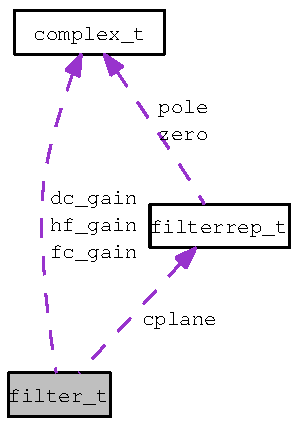
\includegraphics[width=89pt]{structfilter__t__coll__graph}
\end{center}
\end{figure}


\subsubsection{Detailed Description}
The filter structure. 

Definition at line 437 of file bpm\_\-dsp.h.\subsubsection*{Data Fields}
\begin{CompactItemize}
\item 
char {\bf name} [80]
\item 
unsigned int {\bf options}
\item 
int {\bf order}
\item 
double {\bf fs}
\item 
double {\bf f1}
\item 
double {\bf f2}
\item 
double {\bf alpha1}
\item 
double {\bf alpha2}
\item 
double {\bf w\_\-alpha1}
\item 
double {\bf w\_\-alpha2}
\item 
double {\bf cheb\_\-ripple}
\item 
double {\bf Q}
\item 
double {\bf gauss\_\-cutoff}
\item 
{\bf complex\_\-t} {\bf dc\_\-gain}
\item 
{\bf complex\_\-t} {\bf fc\_\-gain}
\item 
{\bf complex\_\-t} {\bf hf\_\-gain}
\item 
double {\bf gain}
\item 
{\bf filterrep\_\-t} $\ast$ {\bf cplane}
\item 
int {\bf nxc}
\item 
double {\bf xc} [MAXPZ+1]
\item 
int {\bf nxc\_\-ac}
\item 
double {\bf xc\_\-ac} [MAXPZ+1]
\item 
int {\bf nyc}
\item 
double {\bf yc} [MAXPZ+1]
\item 
int {\bf nyc\_\-ac}
\item 
double {\bf yc\_\-ac} [MAXPZ+1]
\item 
double {\bf xv} [MAXPZ+1]
\item 
double {\bf xv\_\-ac} [MAXPZ+1]
\item 
double {\bf yv} [MAXPZ+1]
\item 
double {\bf yv\_\-ac} [MAXPZ+1]
\item 
int {\bf ns}
\item 
double $\ast$ {\bf wfbuffer}
\end{CompactItemize}


\subsubsection{Field Documentation}
\index{filter\_\-t@{filter\_\-t}!name@{name}}
\index{name@{name}!filter_t@{filter\_\-t}}
\paragraph[name]{\setlength{\rightskip}{0pt plus 5cm}char {\bf filter\_\-t::name}[80]}\hfill\label{structfilter__t_420d5f6fd6f7b83fb674fe5a81c18425}


The filter's name 

Definition at line 438 of file bpm\_\-dsp.h.

Referenced by create\_\-filter(), and print\_\-filter().\index{filter\_\-t@{filter\_\-t}!options@{options}}
\index{options@{options}!filter_t@{filter\_\-t}}
\paragraph[options]{\setlength{\rightskip}{0pt plus 5cm}unsigned int {\bf filter\_\-t::options}}\hfill\label{structfilter__t_f1f1d9266ba72eda6685c631f4dde41f}


type and option bits for filter 

Definition at line 440 of file bpm\_\-dsp.h.

Referenced by apply\_\-filter(), calculate\_\-filter\_\-coefficients(), create\_\-filter(), create\_\-resonator\_\-representation(), create\_\-splane\_\-representation(), gaussian\_\-filter\_\-coeffs(), normalise\_\-filter(), print\_\-filter(), and zplane\_\-transform().\index{filter\_\-t@{filter\_\-t}!order@{order}}
\index{order@{order}!filter_t@{filter\_\-t}}
\paragraph[order]{\setlength{\rightskip}{0pt plus 5cm}int {\bf filter\_\-t::order}}\hfill\label{structfilter__t_300a7f45bc8727f2c77cf1d9845deb96}


filter order 

Definition at line 441 of file bpm\_\-dsp.h.

Referenced by create\_\-filter(), and create\_\-splane\_\-representation().\index{filter\_\-t@{filter\_\-t}!fs@{fs}}
\index{fs@{fs}!filter_t@{filter\_\-t}}
\paragraph[fs]{\setlength{\rightskip}{0pt plus 5cm}double {\bf filter\_\-t::fs}}\hfill\label{structfilter__t_fcb71153474c026e4af9eb79e134272c}


sampling frequency 

Definition at line 443 of file bpm\_\-dsp.h.

Referenced by create\_\-filter(), and gaussian\_\-filter\_\-coeffs().\index{filter\_\-t@{filter\_\-t}!f1@{f1}}
\index{f1@{f1}!filter_t@{filter\_\-t}}
\paragraph[f1]{\setlength{\rightskip}{0pt plus 5cm}double {\bf filter\_\-t::f1}}\hfill\label{structfilter__t_ee11cdb8bd177a80af5a8145ef2994a7}


first frequency ( left edge for bandpass/stop ) 

Definition at line 444 of file bpm\_\-dsp.h.

Referenced by create\_\-filter(), and gaussian\_\-filter\_\-coeffs().\index{filter\_\-t@{filter\_\-t}!f2@{f2}}
\index{f2@{f2}!filter_t@{filter\_\-t}}
\paragraph[f2]{\setlength{\rightskip}{0pt plus 5cm}double {\bf filter\_\-t::f2}}\hfill\label{structfilter__t_f20ed86d13f7d772b34d24fdad574d98}


right edge for bandpass/stop ( undef for low/highpass ) 

Definition at line 445 of file bpm\_\-dsp.h.

Referenced by create\_\-filter().\index{filter\_\-t@{filter\_\-t}!alpha1@{alpha1}}
\index{alpha1@{alpha1}!filter_t@{filter\_\-t}}
\paragraph[alpha1]{\setlength{\rightskip}{0pt plus 5cm}double {\bf filter\_\-t::alpha1}}\hfill\label{structfilter__t_cc6b5340d5c29772295c9e9a77996875}


rescaled f1 

Definition at line 447 of file bpm\_\-dsp.h.

Referenced by calculate\_\-filter\_\-coefficients(), create\_\-filter(), and create\_\-resonator\_\-representation().\index{filter\_\-t@{filter\_\-t}!alpha2@{alpha2}}
\index{alpha2@{alpha2}!filter_t@{filter\_\-t}}
\paragraph[alpha2]{\setlength{\rightskip}{0pt plus 5cm}double {\bf filter\_\-t::alpha2}}\hfill\label{structfilter__t_8124f521ac4d25e9afbca612f8afa202}


rescaled f2 

Definition at line 448 of file bpm\_\-dsp.h.

Referenced by calculate\_\-filter\_\-coefficients(), and create\_\-filter().\index{filter\_\-t@{filter\_\-t}!w\_\-alpha1@{w\_\-alpha1}}
\index{w\_\-alpha1@{w\_\-alpha1}!filter_t@{filter\_\-t}}
\paragraph[w\_\-alpha1]{\setlength{\rightskip}{0pt plus 5cm}double {\bf filter\_\-t::w\_\-alpha1}}\hfill\label{structfilter__t_dc08473e572d2bb1b6442d7ccda22d7a}


warped alpha1 

Definition at line 450 of file bpm\_\-dsp.h.

Referenced by create\_\-filter(), and normalise\_\-filter().\index{filter\_\-t@{filter\_\-t}!w\_\-alpha2@{w\_\-alpha2}}
\index{w\_\-alpha2@{w\_\-alpha2}!filter_t@{filter\_\-t}}
\paragraph[w\_\-alpha2]{\setlength{\rightskip}{0pt plus 5cm}double {\bf filter\_\-t::w\_\-alpha2}}\hfill\label{structfilter__t_b1712c2f6e445670dd8e4063f2e281ad}


warped alpha2 

Definition at line 451 of file bpm\_\-dsp.h.

Referenced by create\_\-filter(), and normalise\_\-filter().\index{filter\_\-t@{filter\_\-t}!cheb\_\-ripple@{cheb\_\-ripple}}
\index{cheb\_\-ripple@{cheb\_\-ripple}!filter_t@{filter\_\-t}}
\paragraph[cheb\_\-ripple]{\setlength{\rightskip}{0pt plus 5cm}double {\bf filter\_\-t::cheb\_\-ripple}}\hfill\label{structfilter__t_674643ee7b183192df19cd3cd7e38a3d}


ripple for chebyshev filters 

Definition at line 453 of file bpm\_\-dsp.h.

Referenced by create\_\-filter(), and create\_\-splane\_\-representation().\index{filter\_\-t@{filter\_\-t}!Q@{Q}}
\index{Q@{Q}!filter_t@{filter\_\-t}}
\paragraph[Q]{\setlength{\rightskip}{0pt plus 5cm}double {\bf filter\_\-t::Q}}\hfill\label{structfilter__t_1a2c1f97d417a58cb58346906afc8205}


Q factor for resonators 

Definition at line 454 of file bpm\_\-dsp.h.

Referenced by create\_\-filter(), and create\_\-resonator\_\-representation().\index{filter\_\-t@{filter\_\-t}!gauss\_\-cutoff@{gauss\_\-cutoff}}
\index{gauss\_\-cutoff@{gauss\_\-cutoff}!filter_t@{filter\_\-t}}
\paragraph[gauss\_\-cutoff]{\setlength{\rightskip}{0pt plus 5cm}double {\bf filter\_\-t::gauss\_\-cutoff}}\hfill\label{structfilter__t_bb943262c0d73b7dc911fc5ec4f155a6}


gaussian filter cutoff parameter 

Definition at line 455 of file bpm\_\-dsp.h.

Referenced by create\_\-filter(), and gaussian\_\-filter\_\-coeffs().\index{filter\_\-t@{filter\_\-t}!dc\_\-gain@{dc\_\-gain}}
\index{dc\_\-gain@{dc\_\-gain}!filter_t@{filter\_\-t}}
\paragraph[dc\_\-gain]{\setlength{\rightskip}{0pt plus 5cm}{\bf complex\_\-t} {\bf filter\_\-t::dc\_\-gain}}\hfill\label{structfilter__t_1fb8ef235aebd042e645d032a45e71df}


Complex DC gain of the filter 

Definition at line 457 of file bpm\_\-dsp.h.

Referenced by calculate\_\-filter\_\-coefficients(), and print\_\-filter().\index{filter\_\-t@{filter\_\-t}!fc\_\-gain@{fc\_\-gain}}
\index{fc\_\-gain@{fc\_\-gain}!filter_t@{filter\_\-t}}
\paragraph[fc\_\-gain]{\setlength{\rightskip}{0pt plus 5cm}{\bf complex\_\-t} {\bf filter\_\-t::fc\_\-gain}}\hfill\label{structfilter__t_be3e7477ffd82a35ab7c0e7dcdc4a314}


Complex Center frequency gain of filter 

Definition at line 458 of file bpm\_\-dsp.h.

Referenced by calculate\_\-filter\_\-coefficients(), and print\_\-filter().\index{filter\_\-t@{filter\_\-t}!hf\_\-gain@{hf\_\-gain}}
\index{hf\_\-gain@{hf\_\-gain}!filter_t@{filter\_\-t}}
\paragraph[hf\_\-gain]{\setlength{\rightskip}{0pt plus 5cm}{\bf complex\_\-t} {\bf filter\_\-t::hf\_\-gain}}\hfill\label{structfilter__t_a383fcf8e8345bd268d40a374276bb0f}


Complex High frequency (fNy) gain of filter 

Definition at line 459 of file bpm\_\-dsp.h.

Referenced by calculate\_\-filter\_\-coefficients(), and print\_\-filter().\index{filter\_\-t@{filter\_\-t}!gain@{gain}}
\index{gain@{gain}!filter_t@{filter\_\-t}}
\paragraph[gain]{\setlength{\rightskip}{0pt plus 5cm}double {\bf filter\_\-t::gain}}\hfill\label{structfilter__t_9f8ff8688cc79f123f63209d62073677}


Actual Filter gain 

Definition at line 460 of file bpm\_\-dsp.h.

Referenced by apply\_\-filter(), calculate\_\-filter\_\-coefficients(), gaussian\_\-filter\_\-coeffs(), and print\_\-filter().\index{filter\_\-t@{filter\_\-t}!cplane@{cplane}}
\index{cplane@{cplane}!filter_t@{filter\_\-t}}
\paragraph[cplane]{\setlength{\rightskip}{0pt plus 5cm}{\bf filterrep\_\-t}$\ast$ {\bf filter\_\-t::cplane}}\hfill\label{structfilter__t_d60ad283b3847bcf61069cb0aecb3a84}


pointer to complex filter representation, poles and zeros 

Definition at line 462 of file bpm\_\-dsp.h.

Referenced by calculate\_\-filter\_\-coefficients(), create\_\-filter(), delete\_\-filter(), and print\_\-filter().\index{filter\_\-t@{filter\_\-t}!nxc@{nxc}}
\index{nxc@{nxc}!filter_t@{filter\_\-t}}
\paragraph[nxc]{\setlength{\rightskip}{0pt plus 5cm}int {\bf filter\_\-t::nxc}}\hfill\label{structfilter__t_0a4cebb1e641ab50077f260ad11c7788}


number of x coefficients 

Definition at line 464 of file bpm\_\-dsp.h.

Referenced by apply\_\-filter(), calculate\_\-filter\_\-coefficients(), gaussian\_\-filter\_\-coeffs(), and print\_\-filter().\index{filter\_\-t@{filter\_\-t}!xc@{xc}}
\index{xc@{xc}!filter_t@{filter\_\-t}}
\paragraph[xc]{\setlength{\rightskip}{0pt plus 5cm}double {\bf filter\_\-t::xc}[MAXPZ+1]}\hfill\label{structfilter__t_22b9df0209c051f2ddc148486e7d6f8a}


pointer to array of x coefficients 

Definition at line 465 of file bpm\_\-dsp.h.

Referenced by apply\_\-filter(), calculate\_\-filter\_\-coefficients(), gaussian\_\-filter\_\-coeffs(), and print\_\-filter().\index{filter\_\-t@{filter\_\-t}!nxc\_\-ac@{nxc\_\-ac}}
\index{nxc\_\-ac@{nxc\_\-ac}!filter_t@{filter\_\-t}}
\paragraph[nxc\_\-ac]{\setlength{\rightskip}{0pt plus 5cm}int {\bf filter\_\-t::nxc\_\-ac}}\hfill\label{structfilter__t_92369adf50700705324f0ead36ec800c}


number of anti-causal x coefficients 

Definition at line 467 of file bpm\_\-dsp.h.

Referenced by apply\_\-filter(), gaussian\_\-filter\_\-coeffs(), and print\_\-filter().\index{filter\_\-t@{filter\_\-t}!xc\_\-ac@{xc\_\-ac}}
\index{xc\_\-ac@{xc\_\-ac}!filter_t@{filter\_\-t}}
\paragraph[xc\_\-ac]{\setlength{\rightskip}{0pt plus 5cm}double {\bf filter\_\-t::xc\_\-ac}[MAXPZ+1]}\hfill\label{structfilter__t_7918586bf5ed32660dabe328a1f2589f}


pointer to array of anti-causal x coefficients 

Definition at line 468 of file bpm\_\-dsp.h.

Referenced by apply\_\-filter(), gaussian\_\-filter\_\-coeffs(), and print\_\-filter().\index{filter\_\-t@{filter\_\-t}!nyc@{nyc}}
\index{nyc@{nyc}!filter_t@{filter\_\-t}}
\paragraph[nyc]{\setlength{\rightskip}{0pt plus 5cm}int {\bf filter\_\-t::nyc}}\hfill\label{structfilter__t_b67b5502d78fb69739317f7330d9bf19}


number of y coefficients (for IIR filters) 

Definition at line 470 of file bpm\_\-dsp.h.

Referenced by apply\_\-filter(), calculate\_\-filter\_\-coefficients(), and print\_\-filter().\index{filter\_\-t@{filter\_\-t}!yc@{yc}}
\index{yc@{yc}!filter_t@{filter\_\-t}}
\paragraph[yc]{\setlength{\rightskip}{0pt plus 5cm}double {\bf filter\_\-t::yc}[MAXPZ+1]}\hfill\label{structfilter__t_f90b9fd76e7e0bf377a17ea23ca589f0}


pointer to array of y coefficients 

Definition at line 471 of file bpm\_\-dsp.h.

Referenced by apply\_\-filter(), calculate\_\-filter\_\-coefficients(), create\_\-filter(), and print\_\-filter().\index{filter\_\-t@{filter\_\-t}!nyc\_\-ac@{nyc\_\-ac}}
\index{nyc\_\-ac@{nyc\_\-ac}!filter_t@{filter\_\-t}}
\paragraph[nyc\_\-ac]{\setlength{\rightskip}{0pt plus 5cm}int {\bf filter\_\-t::nyc\_\-ac}}\hfill\label{structfilter__t_0efd9c9142e1de7ed343838b73c6bbca}


number of anti-causal y coefficients (for IIR filters) 

Definition at line 473 of file bpm\_\-dsp.h.\index{filter\_\-t@{filter\_\-t}!yc\_\-ac@{yc\_\-ac}}
\index{yc\_\-ac@{yc\_\-ac}!filter_t@{filter\_\-t}}
\paragraph[yc\_\-ac]{\setlength{\rightskip}{0pt plus 5cm}double {\bf filter\_\-t::yc\_\-ac}[MAXPZ+1]}\hfill\label{structfilter__t_a51fea51992b0ad09ad85a504ce2223e}


pointer to array of anti-causal y coefficients 

Definition at line 474 of file bpm\_\-dsp.h.\index{filter\_\-t@{filter\_\-t}!xv@{xv}}
\index{xv@{xv}!filter_t@{filter\_\-t}}
\paragraph[xv]{\setlength{\rightskip}{0pt plus 5cm}double {\bf filter\_\-t::xv}[MAXPZ+1]}\hfill\label{structfilter__t_26b1836d03ff46c9d76a9129ae225820}


filter x buffer, used in apply\_\-filter 

Definition at line 476 of file bpm\_\-dsp.h.

Referenced by apply\_\-filter().\index{filter\_\-t@{filter\_\-t}!xv\_\-ac@{xv\_\-ac}}
\index{xv\_\-ac@{xv\_\-ac}!filter_t@{filter\_\-t}}
\paragraph[xv\_\-ac]{\setlength{\rightskip}{0pt plus 5cm}double {\bf filter\_\-t::xv\_\-ac}[MAXPZ+1]}\hfill\label{structfilter__t_48fa496d9b7b4c496ae3209a4d8004d6}


filter x buffer, used in apply\_\-filter 

Definition at line 477 of file bpm\_\-dsp.h.

Referenced by apply\_\-filter().\index{filter\_\-t@{filter\_\-t}!yv@{yv}}
\index{yv@{yv}!filter_t@{filter\_\-t}}
\paragraph[yv]{\setlength{\rightskip}{0pt plus 5cm}double {\bf filter\_\-t::yv}[MAXPZ+1]}\hfill\label{structfilter__t_7c459fa3bbf050e6a2521cd5f7542f5d}


filter y buffer, used in apply\_\-filter 

Definition at line 479 of file bpm\_\-dsp.h.

Referenced by apply\_\-filter().\index{filter\_\-t@{filter\_\-t}!yv\_\-ac@{yv\_\-ac}}
\index{yv\_\-ac@{yv\_\-ac}!filter_t@{filter\_\-t}}
\paragraph[yv\_\-ac]{\setlength{\rightskip}{0pt plus 5cm}double {\bf filter\_\-t::yv\_\-ac}[MAXPZ+1]}\hfill\label{structfilter__t_71a724a67ac888e6aaebc3962d82b3aa}


filter y buffer, used in apply\_\-filter 

Definition at line 480 of file bpm\_\-dsp.h.

Referenced by apply\_\-filter().\index{filter\_\-t@{filter\_\-t}!ns@{ns}}
\index{ns@{ns}!filter_t@{filter\_\-t}}
\paragraph[ns]{\setlength{\rightskip}{0pt plus 5cm}int {\bf filter\_\-t::ns}}\hfill\label{structfilter__t_f90dc219ac95f6b1723622a4b7946b93}


number of samples of waveforms to be filtered 

Definition at line 482 of file bpm\_\-dsp.h.

Referenced by apply\_\-filter(), create\_\-filter(), filter\_\-impulse\_\-response(), filter\_\-step\_\-response(), and gaussian\_\-filter\_\-coeffs().\index{filter\_\-t@{filter\_\-t}!wfbuffer@{wfbuffer}}
\index{wfbuffer@{wfbuffer}!filter_t@{filter\_\-t}}
\paragraph[wfbuffer]{\setlength{\rightskip}{0pt plus 5cm}double$\ast$ {\bf filter\_\-t::wfbuffer}}\hfill\label{structfilter__t_d5ac1b6a82e84bbcda0b70c56a1011a6}


waveform buffer for filter computations, allocated once ! 

Definition at line 483 of file bpm\_\-dsp.h.

Referenced by apply\_\-filter(), create\_\-filter(), and delete\_\-filter().

The documentation for this struct was generated from the following file:\begin{CompactItemize}
\item 
bpmdsp/{\bf bpm\_\-dsp.h}\end{CompactItemize}

\subsection{filterrep\_\-t Struct Reference}
\label{structfilterrep__t}\index{filterrep\_\-t@{filterrep\_\-t}}
{\tt \#include $<$bpm\_\-dsp.h$>$}

Collaboration diagram for filterrep\_\-t:\nopagebreak
\begin{figure}[H]
\begin{center}
\leavevmode
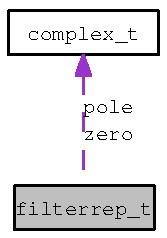
\includegraphics[width=58pt]{structfilterrep__t__coll__graph}
\end{center}
\end{figure}


\subsubsection{Detailed Description}
The filter representation in the complex plane (poles/zeros). 

Definition at line 427 of file bpm\_\-dsp.h.\subsubsection*{Data Fields}
\begin{CompactItemize}
\item 
int {\bf npoles}
\item 
int {\bf nzeros}
\item 
{\bf complex\_\-t} {\bf pole} [MAXPZ]
\item 
{\bf complex\_\-t} {\bf zero} [MAXPZ]
\end{CompactItemize}


\subsubsection{Field Documentation}
\index{filterrep\_\-t@{filterrep\_\-t}!npoles@{npoles}}
\index{npoles@{npoles}!filterrep_t@{filterrep\_\-t}}
\paragraph[npoles]{\setlength{\rightskip}{0pt plus 5cm}int {\bf filterrep\_\-t::npoles}}\hfill\label{structfilterrep__t_696051b6536b2d1416a6fd035998d402}


The number of filter poles 

Definition at line 428 of file bpm\_\-dsp.h.

Referenced by calculate\_\-filter\_\-coefficients(), create\_\-filter(), create\_\-resonator\_\-representation(), create\_\-splane\_\-representation(), normalise\_\-filter(), print\_\-filter\_\-representation(), and zplane\_\-transform().\index{filterrep\_\-t@{filterrep\_\-t}!nzeros@{nzeros}}
\index{nzeros@{nzeros}!filterrep_t@{filterrep\_\-t}}
\paragraph[nzeros]{\setlength{\rightskip}{0pt plus 5cm}int {\bf filterrep\_\-t::nzeros}}\hfill\label{structfilterrep__t_c3b88e769143d340f94320a2096170ae}


The number of filter zeros 

Definition at line 429 of file bpm\_\-dsp.h.

Referenced by calculate\_\-filter\_\-coefficients(), create\_\-resonator\_\-representation(), normalise\_\-filter(), print\_\-filter\_\-representation(), and zplane\_\-transform().\index{filterrep\_\-t@{filterrep\_\-t}!pole@{pole}}
\index{pole@{pole}!filterrep_t@{filterrep\_\-t}}
\paragraph[pole]{\setlength{\rightskip}{0pt plus 5cm}{\bf complex\_\-t} {\bf filterrep\_\-t::pole}[MAXPZ]}\hfill\label{structfilterrep__t_6e09dea05781f890ca586f44a23811b4}


Array of the filter's complex poles 

Definition at line 430 of file bpm\_\-dsp.h.

Referenced by calculate\_\-filter\_\-coefficients(), create\_\-resonator\_\-representation(), create\_\-splane\_\-representation(), normalise\_\-filter(), print\_\-filter\_\-representation(), and zplane\_\-transform().\index{filterrep\_\-t@{filterrep\_\-t}!zero@{zero}}
\index{zero@{zero}!filterrep_t@{filterrep\_\-t}}
\paragraph[zero]{\setlength{\rightskip}{0pt plus 5cm}{\bf complex\_\-t} {\bf filterrep\_\-t::zero}[MAXPZ]}\hfill\label{structfilterrep__t_41c194dbef24dc71cd25a7cd9821c7ac}


Array of the filter's complex zeros 

Definition at line 431 of file bpm\_\-dsp.h.

Referenced by calculate\_\-filter\_\-coefficients(), create\_\-resonator\_\-representation(), normalise\_\-filter(), print\_\-filter\_\-representation(), and zplane\_\-transform().

The documentation for this struct was generated from the following file:\begin{CompactItemize}
\item 
bpmdsp/{\bf bpm\_\-dsp.h}\end{CompactItemize}

\subsection{intwf\_\-t Struct Reference}
\label{structintwf__t}\index{intwf\_\-t@{intwf\_\-t}}
{\tt \#include $<$bpm\_\-wf.h$>$}



\subsubsection{Detailed Description}
Structure representing a waveform of integers 

Definition at line 181 of file bpm\_\-wf.h.\subsubsection*{Data Fields}
\begin{CompactItemize}
\item 
int {\bf ns}
\item 
double {\bf fs}
\item 
int $\ast$ {\bf wf}
\end{CompactItemize}


\subsubsection{Field Documentation}
\index{intwf\_\-t@{intwf\_\-t}!ns@{ns}}
\index{ns@{ns}!intwf_t@{intwf\_\-t}}
\paragraph[ns]{\setlength{\rightskip}{0pt plus 5cm}int {\bf intwf\_\-t::ns}}\hfill\label{structintwf__t_803ea4f9dabd4fb7c7f5bb331f6525f1}


The number of samples in the waveform 

Definition at line 182 of file bpm\_\-wf.h.

Referenced by digitise(), doublewf\_\-cast(), doublewf\_\-cast\_\-new(), intwf(), intwf\_\-add(), intwf\_\-add\_\-ampnoise(), intwf\_\-add\_\-cwtone(), intwf\_\-add\_\-dcywave(), intwf\_\-bias(), intwf\_\-cast(), intwf\_\-cast\_\-new(), intwf\_\-compat(), intwf\_\-copy(), intwf\_\-copy\_\-new(), intwf\_\-derive(), intwf\_\-divide(), intwf\_\-integrate(), intwf\_\-multiply(), intwf\_\-print(), intwf\_\-resample(), intwf\_\-reset(), intwf\_\-sample\_\-series(), intwf\_\-scale(), intwf\_\-setvalues(), intwf\_\-subset(), and intwf\_\-subtract().\index{intwf\_\-t@{intwf\_\-t}!fs@{fs}}
\index{fs@{fs}!intwf_t@{intwf\_\-t}}
\paragraph[fs]{\setlength{\rightskip}{0pt plus 5cm}double {\bf intwf\_\-t::fs}}\hfill\label{structintwf__t_b0d66ade539e6f2440357e540716a49f}


The sampling frequency 

Definition at line 183 of file bpm\_\-wf.h.

Referenced by digitise(), doublewf\_\-cast\_\-new(), intwf(), intwf\_\-add\_\-cwtone(), intwf\_\-add\_\-dcywave(), intwf\_\-compat(), intwf\_\-copy\_\-new(), intwf\_\-derive(), intwf\_\-integrate(), intwf\_\-print(), intwf\_\-resample(), and intwf\_\-subset().\index{intwf\_\-t@{intwf\_\-t}!wf@{wf}}
\index{wf@{wf}!intwf_t@{intwf\_\-t}}
\paragraph[wf]{\setlength{\rightskip}{0pt plus 5cm}int$\ast$ {\bf intwf\_\-t::wf}}\hfill\label{structintwf__t_3fa321b84fdc1ccd3c4bcd789da5b95c}


Pointer to an array of integers which hold the samples 

Definition at line 184 of file bpm\_\-wf.h.

Referenced by digitise(), doublewf\_\-cast(), doublewf\_\-cast\_\-new(), intwf(), intwf\_\-add(), intwf\_\-add\_\-ampnoise(), intwf\_\-add\_\-cwtone(), intwf\_\-add\_\-dcywave(), intwf\_\-bias(), intwf\_\-cast(), intwf\_\-cast\_\-new(), intwf\_\-copy(), intwf\_\-copy\_\-new(), intwf\_\-delete(), intwf\_\-derive(), intwf\_\-divide(), intwf\_\-integrate(), intwf\_\-multiply(), intwf\_\-print(), intwf\_\-resample(), intwf\_\-reset(), intwf\_\-sample\_\-series(), intwf\_\-scale(), intwf\_\-setvalues(), intwf\_\-subset(), and intwf\_\-subtract().

The documentation for this struct was generated from the following file:\begin{CompactItemize}
\item 
bpmwf/{\bf bpm\_\-wf.h}\end{CompactItemize}

\subsection{lm\_\-fstate Struct Reference}
\label{structlm__fstate}\index{lm\_\-fstate@{lm\_\-fstate}}
{\tt \#include $<$bpm\_\-nr.h$>$}



\subsubsection{Detailed Description}
structure needed for levenberg marquard minimisation 

Definition at line 118 of file bpm\_\-nr.h.\subsubsection*{Data Fields}
\begin{CompactItemize}
\item 
int \textbf{n}\label{structlm__fstate_f449b83ccdcf43aaf8cbd3ac0c9ae160}

\item 
int $\ast$ \textbf{nfev}\label{structlm__fstate_91004879d4efbec023c0b8c317487384}

\item 
double $\ast$ \textbf{hx}\label{structlm__fstate_88d7955ba2ae804c6aad61dcd996e4dc}

\item 
double $\ast$ \textbf{x}\label{structlm__fstate_4f93b5b8d96a473d92cf075cec85c935}

\item 
void $\ast$ \textbf{adata}\label{structlm__fstate_26ef87f16e5d54eca25e0675cd0051dc}

\end{CompactItemize}


The documentation for this struct was generated from the following file:\begin{CompactItemize}
\item 
bpmnr/{\bf bpm\_\-nr.h}\end{CompactItemize}

\subsection{m33 Struct Reference}
\label{structm33}\index{m33@{m33}}
{\tt \#include $<$bpm\_\-orbit.h$>$}



\subsubsection{Detailed Description}
Structure representing a 3x3-matrix, for use in the orbit generation routines 

Definition at line 49 of file bpm\_\-orbit.h.\subsubsection*{Data Fields}
\begin{CompactItemize}
\item 
double {\bf e} [3][3]
\end{CompactItemize}


\subsubsection{Field Documentation}
\index{m33@{m33}!e@{e}}
\index{e@{e}!m33@{m33}}
\paragraph[e]{\setlength{\rightskip}{0pt plus 5cm}double {\bf m33::e}[3][3]}\hfill\label{structm33_ff2fb431dec7f3e99fa12f760e855651}


the matrix 

Definition at line 50 of file bpm\_\-orbit.h.

Referenced by generate\_\-diodesignal(), m\_\-matadd(), m\_\-matmult(), m\_\-print(), m\_\-rotmat(), and v\_\-matmult().

The documentation for this struct was generated from the following file:\begin{CompactItemize}
\item 
bpmorbit/{\bf bpm\_\-orbit.h}\end{CompactItemize}

\subsection{rfmodel Struct Reference}
\label{structrfmodel}\index{rfmodel@{rfmodel}}
{\tt \#include $<$bpm\_\-interface.h$>$}

Collaboration diagram for rfmodel:\nopagebreak
\begin{figure}[H]
\begin{center}
\leavevmode
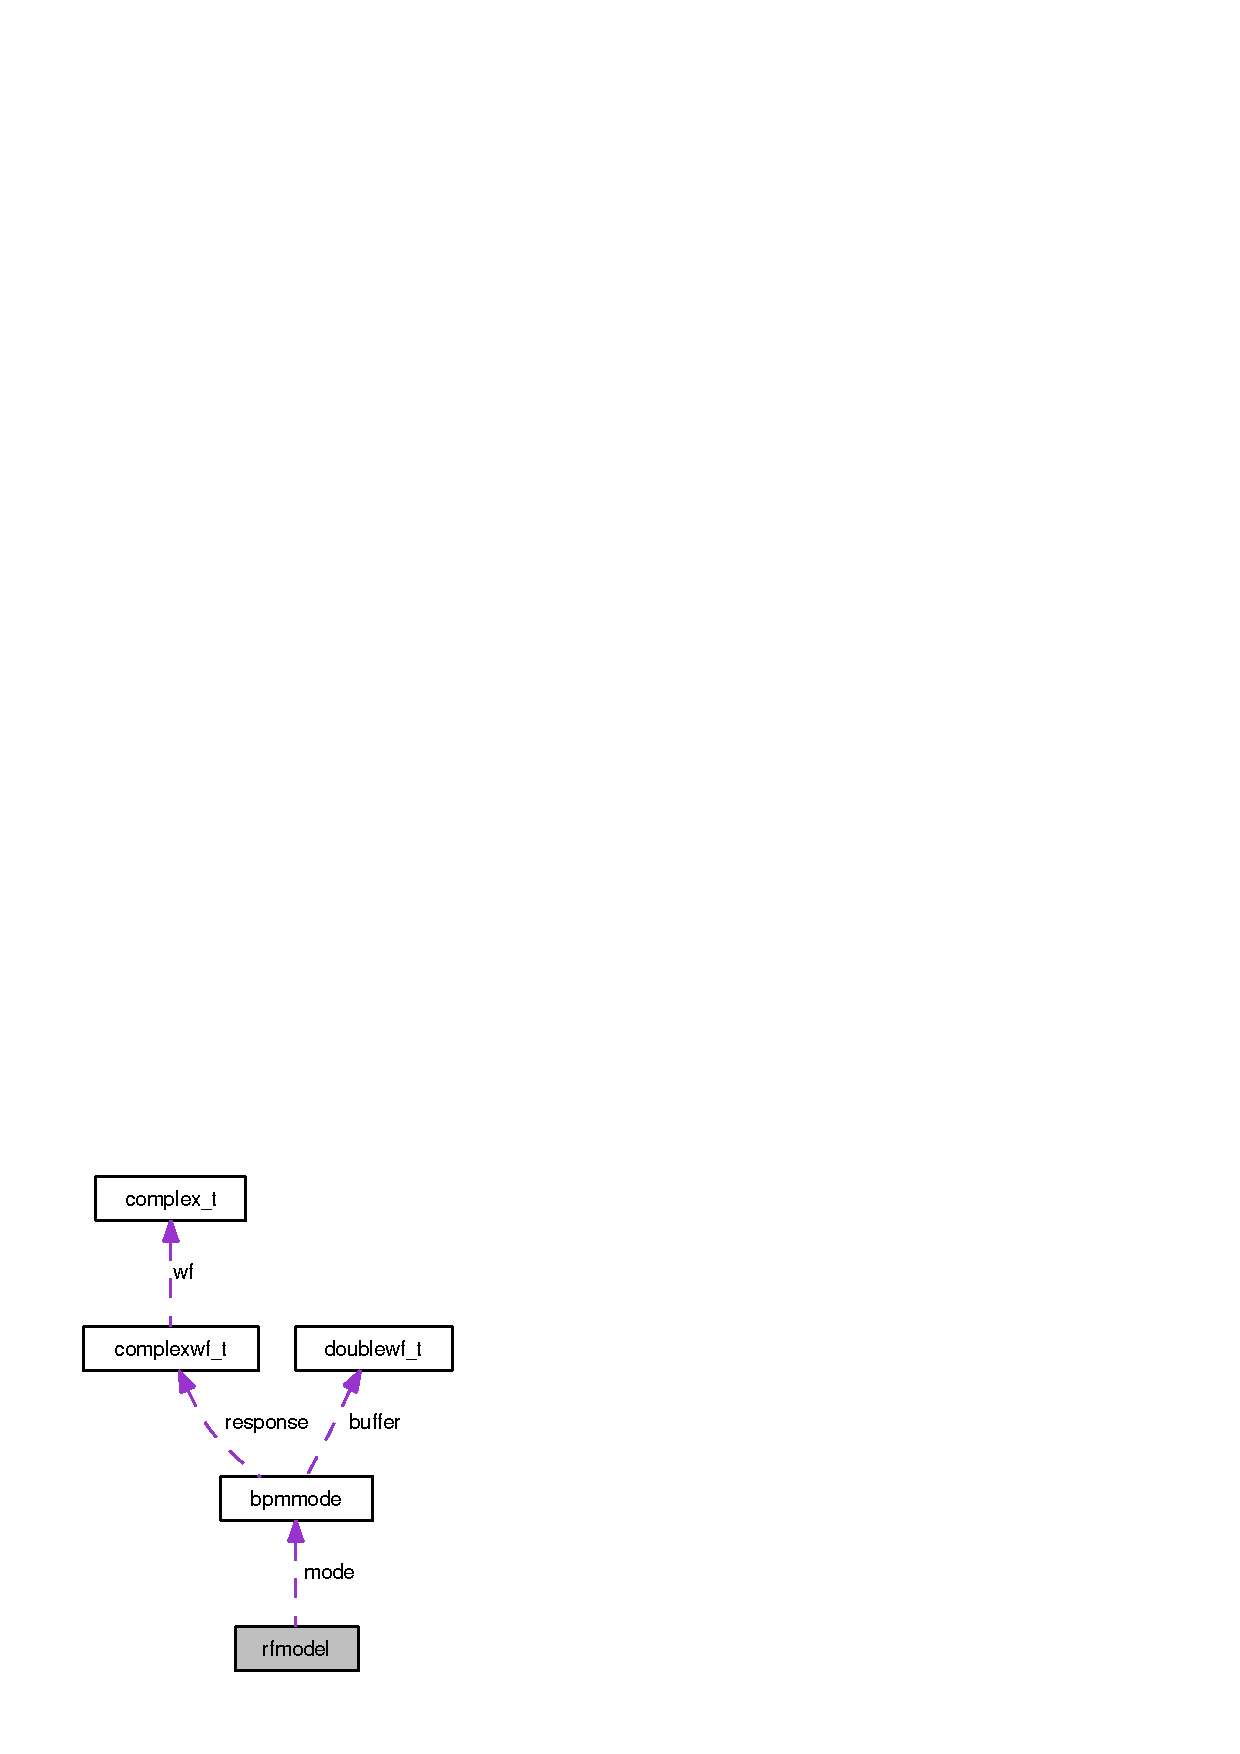
\includegraphics[width=110pt]{structrfmodel__coll__graph}
\end{center}
\end{figure}


\subsubsection{Detailed Description}
This structure contains the complete RF model for a BPM, which is essentially a collection of it's resonant modes and sensitivities 

Definition at line 296 of file bpm\_\-interface.h.\subsubsection*{Data Fields}
\begin{CompactItemize}
\item 
char {\bf name} [20]
\item 
int {\bf nmodes}
\item 
{\bf bpmmode\_\-t} $\ast$ {\bf mode}
\end{CompactItemize}


\subsubsection{Field Documentation}
\index{rfmodel@{rfmodel}!name@{name}}
\index{name@{name}!rfmodel@{rfmodel}}
\paragraph[name]{\setlength{\rightskip}{0pt plus 5cm}char {\bf rfmodel::name}[20]}\hfill\label{structrfmodel_0347645ae53fe9060133b86a13dff957}


A name for the cavity's RF model 

Definition at line 297 of file bpm\_\-interface.h.\index{rfmodel@{rfmodel}!nmodes@{nmodes}}
\index{nmodes@{nmodes}!rfmodel@{rfmodel}}
\paragraph[nmodes]{\setlength{\rightskip}{0pt plus 5cm}int {\bf rfmodel::nmodes}}\hfill\label{structrfmodel_d540be1e4090f1a5f0473ef98924422d}


The number of BPM modes in the model 

Definition at line 298 of file bpm\_\-interface.h.\index{rfmodel@{rfmodel}!mode@{mode}}
\index{mode@{mode}!rfmodel@{rfmodel}}
\paragraph[mode]{\setlength{\rightskip}{0pt plus 5cm}{\bf bpmmode\_\-t}$\ast$ {\bf rfmodel::mode}}\hfill\label{structrfmodel_b4dbc2c56b212e42858185090cfdd0ac}


A list of pointers to the array of modes 

Definition at line 299 of file bpm\_\-interface.h.

The documentation for this struct was generated from the following file:\begin{CompactItemize}
\item 
bpminterface/{\bf bpm\_\-interface.h}\end{CompactItemize}

\subsection{v3 Struct Reference}
\label{structv3}\index{v3@{v3}}
{\tt \#include $<$bpm\_\-orbit.h$>$}



\subsubsection{Detailed Description}
Structure representing a 3-vector, for use in the orbit generation routines 

Definition at line 39 of file bpm\_\-orbit.h.\subsubsection*{Data Fields}
\begin{CompactItemize}
\item 
double {\bf x}
\item 
double {\bf y}
\item 
double {\bf z}
\end{CompactItemize}


\subsubsection{Field Documentation}
\index{v3@{v3}!x@{x}}
\index{x@{x}!v3@{v3}}
\paragraph[x]{\setlength{\rightskip}{0pt plus 5cm}double {\bf v3::x}}\hfill\label{structv3_f2da064a840d85848e931af31332659f}


x-coordinate 

Definition at line 40 of file bpm\_\-orbit.h.

Referenced by get\_\-bpmhit(), v\_\-add(), v\_\-copy(), v\_\-cross(), v\_\-dot(), v\_\-matmult(), v\_\-print(), v\_\-scale(), and v\_\-sub().\index{v3@{v3}!y@{y}}
\index{y@{y}!v3@{v3}}
\paragraph[y]{\setlength{\rightskip}{0pt plus 5cm}double {\bf v3::y}}\hfill\label{structv3_7d96d6103573c71c7b22ecc042eb6a5b}


y-coordinate 

Definition at line 41 of file bpm\_\-orbit.h.

Referenced by get\_\-bpmhit(), v\_\-add(), v\_\-copy(), v\_\-cross(), v\_\-dot(), v\_\-matmult(), v\_\-print(), v\_\-scale(), and v\_\-sub().\index{v3@{v3}!z@{z}}
\index{z@{z}!v3@{v3}}
\paragraph[z]{\setlength{\rightskip}{0pt plus 5cm}double {\bf v3::z}}\hfill\label{structv3_f18ef7bf6197ad38cca46cad49d6636a}


z-coordinate 

Definition at line 42 of file bpm\_\-orbit.h.

Referenced by get\_\-bpmhit(), v\_\-add(), v\_\-copy(), v\_\-cross(), v\_\-dot(), v\_\-matmult(), v\_\-print(), v\_\-scale(), and v\_\-sub().

The documentation for this struct was generated from the following file:\begin{CompactItemize}
\item 
bpmorbit/{\bf bpm\_\-orbit.h}\end{CompactItemize}

\subsection{wfstat\_\-t Struct Reference}
\label{structwfstat__t}\index{wfstat\_\-t@{wfstat\_\-t}}
{\tt \#include $<$bpm\_\-wf.h$>$}



\subsubsection{Detailed Description}
Structure with basic waveform statistics 

Definition at line 196 of file bpm\_\-wf.h.\subsubsection*{Data Fields}
\begin{CompactItemize}
\item 
int {\bf imax}
\item 
int {\bf imin}
\item 
double {\bf max}
\item 
double {\bf min}
\item 
double {\bf mean}
\item 
double {\bf rms}
\end{CompactItemize}


\subsubsection{Field Documentation}
\index{wfstat\_\-t@{wfstat\_\-t}!imax@{imax}}
\index{imax@{imax}!wfstat_t@{wfstat\_\-t}}
\paragraph[imax]{\setlength{\rightskip}{0pt plus 5cm}int {\bf wfstat\_\-t::imax}}\hfill\label{structwfstat__t_f1cdafb6b6193cb959ac93199ee0c89a}


The sample nr of maximum of waveform 

Definition at line 197 of file bpm\_\-wf.h.

Referenced by doublewf\_\-basic\_\-stats(), wfstat\_\-print(), and wfstat\_\-reset().\index{wfstat\_\-t@{wfstat\_\-t}!imin@{imin}}
\index{imin@{imin}!wfstat_t@{wfstat\_\-t}}
\paragraph[imin]{\setlength{\rightskip}{0pt plus 5cm}int {\bf wfstat\_\-t::imin}}\hfill\label{structwfstat__t_a52ebc437733260e378a2fa227c71a6d}


The sample nr of minimum of waveform 

Definition at line 198 of file bpm\_\-wf.h.

Referenced by doublewf\_\-basic\_\-stats(), wfstat\_\-print(), and wfstat\_\-reset().\index{wfstat\_\-t@{wfstat\_\-t}!max@{max}}
\index{max@{max}!wfstat_t@{wfstat\_\-t}}
\paragraph[max]{\setlength{\rightskip}{0pt plus 5cm}double {\bf wfstat\_\-t::max}}\hfill\label{structwfstat__t_ec3cb4f107dea858fff8be1c0674c598}


The maximum value of waveform 

Definition at line 199 of file bpm\_\-wf.h.

Referenced by doublewf\_\-basic\_\-stats(), wfstat\_\-print(), and wfstat\_\-reset().\index{wfstat\_\-t@{wfstat\_\-t}!min@{min}}
\index{min@{min}!wfstat_t@{wfstat\_\-t}}
\paragraph[min]{\setlength{\rightskip}{0pt plus 5cm}double {\bf wfstat\_\-t::min}}\hfill\label{structwfstat__t_3620e9e451fa4b13d7e0ff9b690acd6a}


The minimum value of waveform 

Definition at line 200 of file bpm\_\-wf.h.

Referenced by doublewf\_\-basic\_\-stats(), wfstat\_\-print(), and wfstat\_\-reset().\index{wfstat\_\-t@{wfstat\_\-t}!mean@{mean}}
\index{mean@{mean}!wfstat_t@{wfstat\_\-t}}
\paragraph[mean]{\setlength{\rightskip}{0pt plus 5cm}double {\bf wfstat\_\-t::mean}}\hfill\label{structwfstat__t_04b4e373b3235bef5511c760dc66f4a5}


The mean of waveform 

Definition at line 201 of file bpm\_\-wf.h.

Referenced by doublewf\_\-basic\_\-stats(), get\_\-pedestal(), process\_\-diode(), wfstat\_\-print(), and wfstat\_\-reset().\index{wfstat\_\-t@{wfstat\_\-t}!rms@{rms}}
\index{rms@{rms}!wfstat_t@{wfstat\_\-t}}
\paragraph[rms]{\setlength{\rightskip}{0pt plus 5cm}double {\bf wfstat\_\-t::rms}}\hfill\label{structwfstat__t_715e41714d2b81fb030c27326436bfbb}


The rms of waveform 

Definition at line 202 of file bpm\_\-wf.h.

Referenced by doublewf\_\-basic\_\-stats(), get\_\-pedestal(), process\_\-diode(), wfstat\_\-print(), and wfstat\_\-reset().

The documentation for this struct was generated from the following file:\begin{CompactItemize}
\item 
bpmwf/{\bf bpm\_\-wf.h}\end{CompactItemize}

\section{File Documentation}
\subsection{bpm\_\-units.h File Reference}
\label{bpm__units_8h}\index{bpm\_\-units.h@{bpm\_\-units.h}}


\subsubsection{Detailed Description}
Physical unit definitions for libbpm. 



Definition in file {\bf bpm\_\-units.h}.

{\tt \#include $<$bpm/bpm\_\-defs.h$>$}\par


Include dependency graph for bpm\_\-units.h:\nopagebreak
\begin{figure}[H]
\begin{center}
\leavevmode
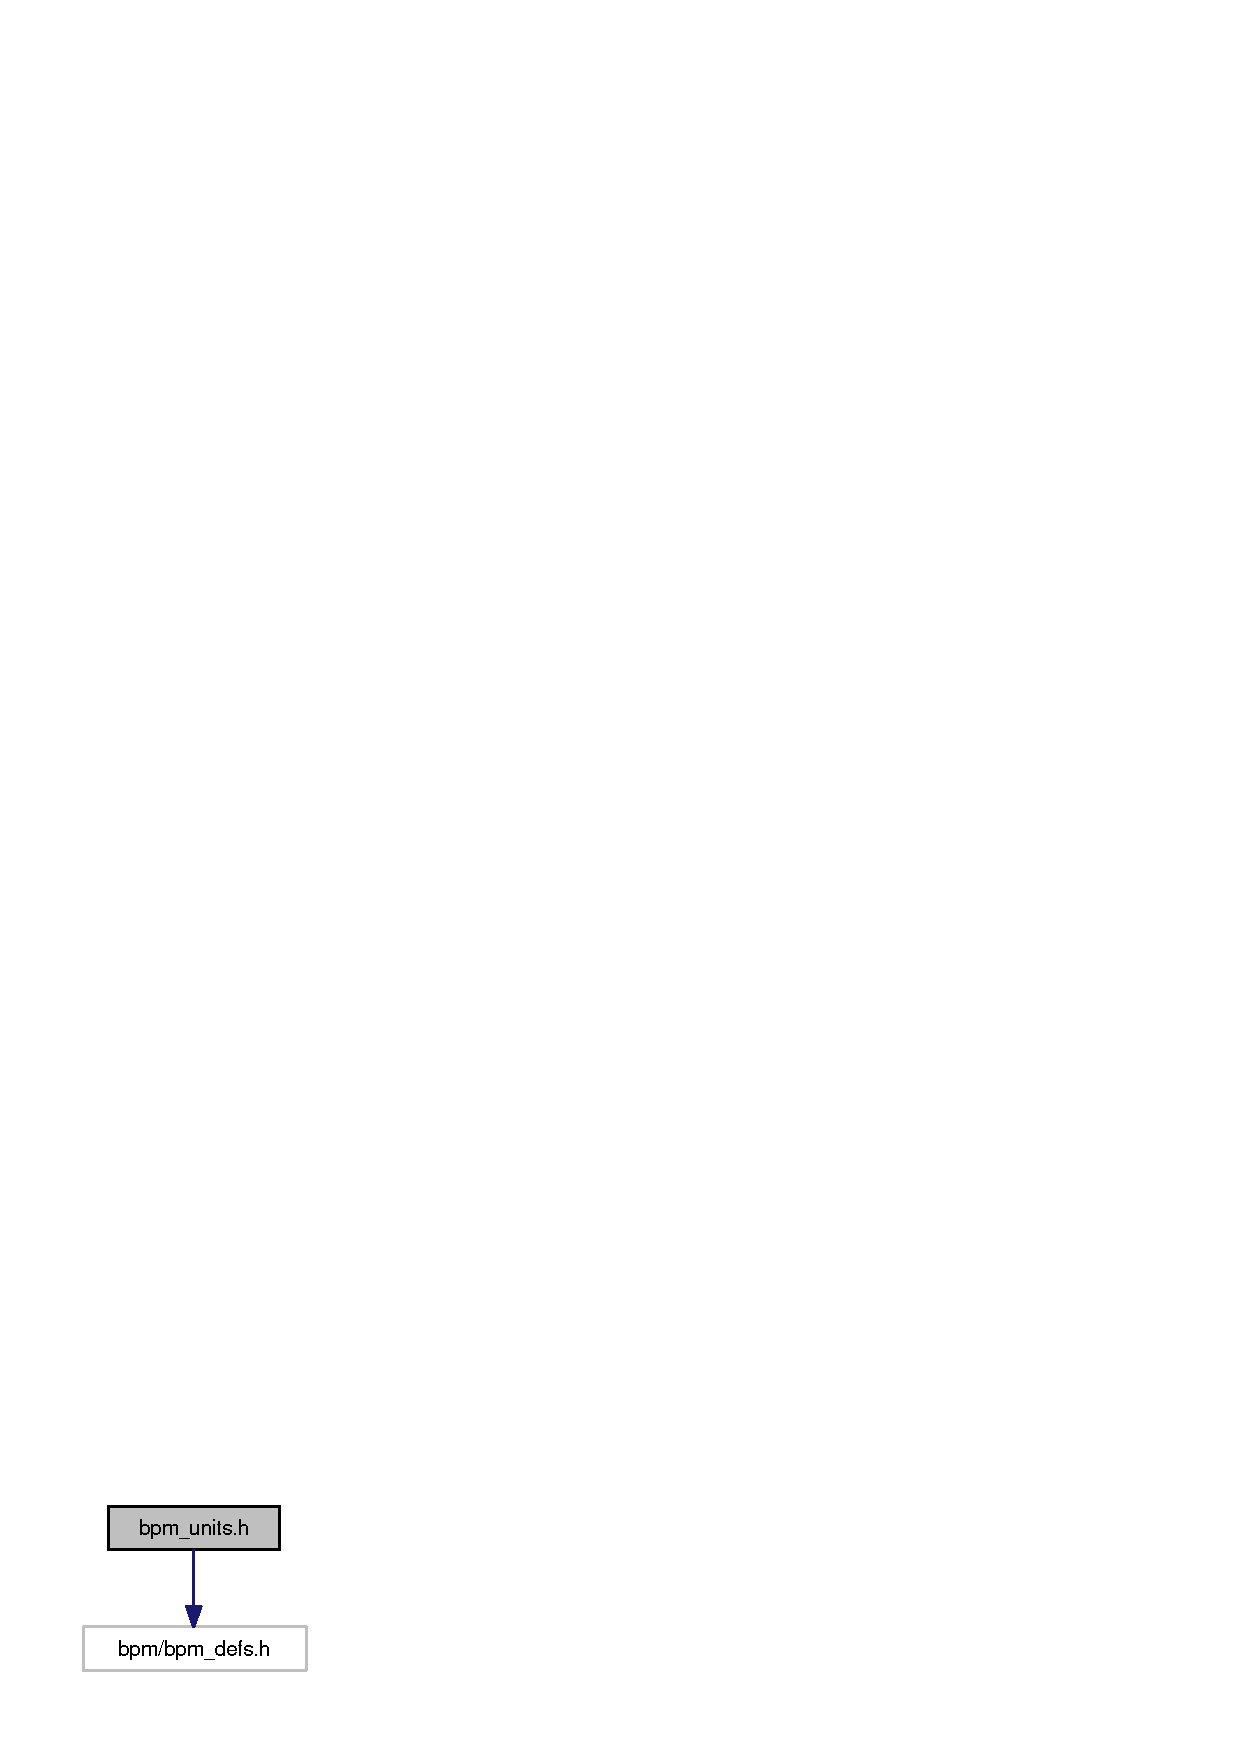
\includegraphics[width=75pt]{bpm__units_8h__incl}
\end{center}
\end{figure}
\subsubsection*{Defines}
\begin{CompactItemize}
\item 
\#define \textbf{\_\-cent\_\-\_\-}\label{bpm__units_8h_c2f27897720a83e5d9474dac8951851b}

\item 
\#define \textbf{\_\-Hz\_\-\_\-}\label{bpm__units_8h_c57ab8c2a60732065d0d3512b4cb9188}

\item 
\#define \textbf{\_\-kHz\_\-\_\-}\label{bpm__units_8h_0ebbaad5a400d7ba82b68128f055ce53}

\item 
\#define \textbf{\_\-MHz\_\-\_\-}\label{bpm__units_8h_922319dd65150e338e4e6c9126a60f81}

\item 
\#define \textbf{\_\-GHz\_\-\_\-}\label{bpm__units_8h_dbe5c54339b443d046f46d2377a808cb}

\item 
\#define \textbf{\_\-sec\_\-\_\-}\label{bpm__units_8h_bfbfa7a22469a4440d1e02bc43cc6615}

\item 
\#define \textbf{\_\-msec\_\-\_\-}\label{bpm__units_8h_a54363851f60be5a02df036353249167}

\item 
\#define \textbf{\_\-usec\_\-\_\-}\label{bpm__units_8h_90a629ff53f070b7dd03b5cd87d319c7}

\item 
\#define \textbf{\_\-nsec\_\-\_\-}\label{bpm__units_8h_893d2e7473157813593484c99d9c6211}

\item 
\#define \textbf{\_\-eV\_\-\_\-}\label{bpm__units_8h_30737d7facf39b26a89729d9039c8405}

\item 
\#define \textbf{\_\-keV\_\-\_\-}\label{bpm__units_8h_80e0bc381ee56da0c7eafd51e19da244}

\item 
\#define \textbf{\_\-MeV\_\-\_\-}\label{bpm__units_8h_af7586a4c5c9e9e3160fae3be37dd025}

\item 
\#define \textbf{\_\-GeV\_\-\_\-}\label{bpm__units_8h_1f77efef66be3ec74299798f4c61630f}

\item 
\#define \textbf{\_\-rad\_\-\_\-}\label{bpm__units_8h_2ff9f709eecf1125273f0998095aec96}

\item 
\#define \textbf{\_\-mrad\_\-\_\-}\label{bpm__units_8h_4d6c281cb96e2265c761e2548528b266}

\item 
\#define \textbf{\_\-urad\_\-\_\-}\label{bpm__units_8h_6093ed7c7a103bf9e2fd3972e928fb13}

\item 
\#define \textbf{\_\-nrad\_\-\_\-}\label{bpm__units_8h_798792094a66ffcadcfc530d8acbee46}

\item 
\#define \textbf{\_\-degrees\_\-\_\-}\label{bpm__units_8h_631ddf20ea27e7e69d032bf17d4cade9}

\item 
\#define \textbf{\_\-mC\_\-\_\-}\label{bpm__units_8h_b08b83792d971febbd6badaac28c51d4}

\item 
\#define \textbf{\_\-uC\_\-\_\-}\label{bpm__units_8h_9108dd8cbb5e6db5f664d790016cda8b}

\item 
\#define \textbf{\_\-nC\_\-\_\-}\label{bpm__units_8h_12f5841aa9c4bac2152d6052829ea628}

\item 
\#define \textbf{\_\-pC\_\-\_\-}\label{bpm__units_8h_204e0e0484a2ebd68bbfdcb99e4bf3ea}

\item 
\#define \textbf{\_\-meter\_\-\_\-}\label{bpm__units_8h_89fc3df3aec49ff01cbcfd03947bde8c}

\item 
\#define \textbf{\_\-mmeter\_\-\_\-}\label{bpm__units_8h_cfea46ea9bb29f6cad74814b7cc256aa}

\item 
\#define \textbf{\_\-umeter\_\-\_\-}\label{bpm__units_8h_ff9f057c3538ad8ab5aad28353c762ca}

\item 
\#define \textbf{\_\-nmeter\_\-\_\-}\label{bpm__units_8h_101c2addbeed340f937742d7901ee5bb}

\item 
\#define \textbf{\_\-Volt\_\-\_\-}\label{bpm__units_8h_0b3f5b8ae4eb0b5955472c57982f3cff}

\item 
\#define \textbf{\_\-mVolt\_\-\_\-}\label{bpm__units_8h_30871b3fb170e681b8b3d97bca2baee0}

\item 
\#define \textbf{\_\-uVolt\_\-\_\-}\label{bpm__units_8h_dee9bfcaff1d1c86812ee6bb0b034145}

\item 
\#define \textbf{\_\-nVolt\_\-\_\-}\label{bpm__units_8h_9f057688b7b4bf0d7acdadc23dc69983}

\item 
\#define \textbf{\_\-cLight\_\-\_\-}\label{bpm__units_8h_1911c1e9314a68633c20e549ee08ac9f}

\end{CompactItemize}

\subsection{bpmanalysis/ana\_\-compute\_\-residual.c File Reference}
\label{ana__compute__residual_8c}\index{bpmanalysis/ana\_\-compute\_\-residual.c@{bpmanalysis/ana\_\-compute\_\-residual.c}}


\subsubsection{Detailed Description}


Definition in file {\bf ana\_\-compute\_\-residual.c}.

{\tt \#include $<$bpm/bpm\_\-messages.h$>$}\par
{\tt \#include $<$bpm/bpm\_\-analysis.h$>$}\par


Include dependency graph for ana\_\-compute\_\-residual.c:\nopagebreak
\begin{figure}[H]
\begin{center}
\leavevmode
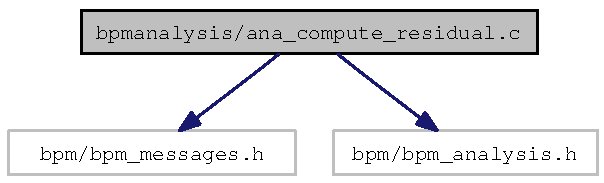
\includegraphics[width=163pt]{ana__compute__residual_8c__incl}
\end{center}
\end{figure}
\subsubsection*{Functions}
\begin{CompactItemize}
\item 
int {\bf ana\_\-compute\_\-residual} ({\bf bpmproc\_\-t} $\ast$$\ast$proc, int num\_\-bpms, int num\_\-evts, double $\ast$coeffs, int mode, double $\ast$mean, double $\ast$rms)
\end{CompactItemize}

\subsection{bpmanalysis/ana\_\-def\_\-cutfn.c File Reference}
\label{ana__def__cutfn_8c}\index{bpmanalysis/ana\_\-def\_\-cutfn.c@{bpmanalysis/ana\_\-def\_\-cutfn.c}}


\subsubsection{Detailed Description}


Definition in file {\bf ana\_\-def\_\-cutfn.c}.

{\tt \#include $<$bpm/bpm\_\-messages.h$>$}\par
{\tt \#include $<$bpm/bpm\_\-analysis.h$>$}\par


Include dependency graph for ana\_\-def\_\-cutfn.c:\nopagebreak
\begin{figure}[H]
\begin{center}
\leavevmode
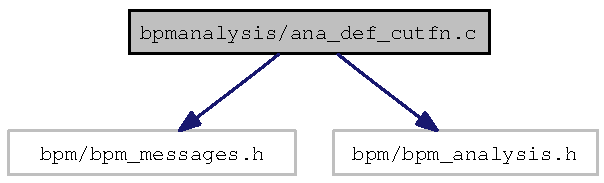
\includegraphics[width=163pt]{ana__def__cutfn_8c__incl}
\end{center}
\end{figure}
\subsubsection*{Functions}
\begin{CompactItemize}
\item 
int {\bf ana\_\-def\_\-cutfn} ({\bf bpmproc\_\-t} $\ast$proc)
\end{CompactItemize}
\subsubsection*{Variables}
\begin{CompactItemize}
\item 
int($\ast$ \textbf{ana\_\-cutfn} )({\bf bpmproc\_\-t} $\ast$proc)\label{ana__def__cutfn_8c_5a54b84177636f0b114cbed86a00643b}

\end{CompactItemize}

\subsection{bpmanalysis/ana\_\-get\_\-svd\_\-coeffs.c File Reference}
\label{ana__get__svd__coeffs_8c}\index{bpmanalysis/ana\_\-get\_\-svd\_\-coeffs.c@{bpmanalysis/ana\_\-get\_\-svd\_\-coeffs.c}}


\subsubsection{Detailed Description}


Definition in file {\bf ana\_\-get\_\-svd\_\-coeffs.c}.

{\tt \#include $<$bpm/bpm\_\-messages.h$>$}\par
{\tt \#include $<$bpm/bpm\_\-analysis.h$>$}\par
{\tt \#include $<$bpm/bpm\_\-nr.h$>$}\par


Include dependency graph for ana\_\-get\_\-svd\_\-coeffs.c:\nopagebreak
\begin{figure}[H]
\begin{center}
\leavevmode
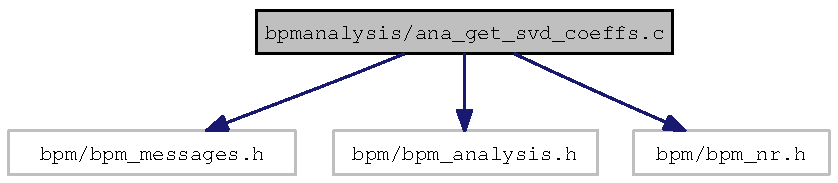
\includegraphics[width=219pt]{ana__get__svd__coeffs_8c__incl}
\end{center}
\end{figure}
\subsubsection*{Functions}
\begin{CompactItemize}
\item 
int {\bf ana\_\-get\_\-svd\_\-coeffs} ({\bf bpmproc\_\-t} $\ast$$\ast$proc, int num\_\-bpms, int num\_\-svd, int total\_\-num\_\-evts, double $\ast$coeffs, int mode)
\end{CompactItemize}

\subsection{bpmanalysis/ana\_\-set\_\-cutfn.c File Reference}
\label{ana__set__cutfn_8c}\index{bpmanalysis/ana\_\-set\_\-cutfn.c@{bpmanalysis/ana\_\-set\_\-cutfn.c}}


\subsubsection{Detailed Description}


Definition in file {\bf ana\_\-set\_\-cutfn.c}.

{\tt \#include $<$bpm/bpm\_\-messages.h$>$}\par
{\tt \#include $<$bpm/bpm\_\-analysis.h$>$}\par


Include dependency graph for ana\_\-set\_\-cutfn.c:\nopagebreak
\begin{figure}[H]
\begin{center}
\leavevmode
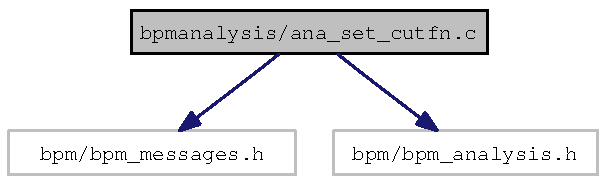
\includegraphics[width=163pt]{ana__set__cutfn_8c__incl}
\end{center}
\end{figure}
\subsubsection*{Functions}
\begin{CompactItemize}
\item 
int {\bf ana\_\-set\_\-cutfn} (int($\ast$cutfn)({\bf bpmproc\_\-t} $\ast$proc))
\end{CompactItemize}

\subsection{bpmanalysis/bpm\_\-analysis.h File Reference}
\label{bpm__analysis_8h}\index{bpmanalysis/bpm\_\-analysis.h@{bpmanalysis/bpm\_\-analysis.h}}


\subsubsection{Detailed Description}
libbpm analysis routines 

This header contains definitions for the libbpm BPM data analysis routines. These mainly are the SVD and resolution/residual calculation routines along with the definition of an analysis cut function... 

Definition in file {\bf bpm\_\-analysis.h}.

{\tt \#include $<$math.h$>$}\par
{\tt \#include $<$bpm/bpm\_\-defs.h$>$}\par
{\tt \#include $<$bpm/bpm\_\-interface.h$>$}\par


Include dependency graph for bpm\_\-analysis.h:\nopagebreak
\begin{figure}[H]
\begin{center}
\leavevmode
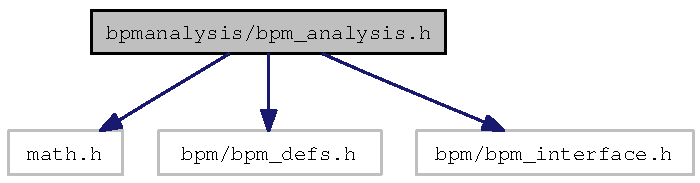
\includegraphics[width=186pt]{bpm__analysis_8h__incl}
\end{center}
\end{figure}
\subsubsection*{Defines}
\begin{CompactItemize}
\item 
\#define {\bf BPM\_\-GOOD\_\-EVENT}
\item 
\#define {\bf BPM\_\-BAD\_\-EVENT}
\item 
\#define {\bf ANA\_\-SVD\_\-TILT}
\item 
\#define {\bf ANA\_\-SVD\_\-NOTILT}
\end{CompactItemize}
\subsubsection*{Functions}
\begin{CompactItemize}
\item 
EXTERN int {\bf ana\_\-set\_\-cutfn} (int($\ast$cutfn)({\bf bpmproc\_\-t} $\ast$proc))
\item 
EXTERN int {\bf ana\_\-get\_\-svd\_\-coeffs} ({\bf bpmproc\_\-t} $\ast$$\ast$proc, int num\_\-bpms, int num\_\-svd, int total\_\-num\_\-evts, double $\ast$coeffs, int mode)
\item 
EXTERN int {\bf ana\_\-compute\_\-residual} ({\bf bpmproc\_\-t} $\ast$$\ast$proc, int num\_\-bpms, int num\_\-evts, double $\ast$coeffs, int mode, double $\ast$mean, double $\ast$rms)
\item 
EXTERN int {\bf ana\_\-def\_\-cutfn} ({\bf bpmproc\_\-t} $\ast$proc)
\end{CompactItemize}
\subsubsection*{Variables}
\begin{CompactItemize}
\item 
EXTERN int($\ast$ {\bf ana\_\-cutfn} )({\bf bpmproc\_\-t} $\ast$proc)
\end{CompactItemize}

\subsection{bpmcalibration/bpm\_\-calibration.h File Reference}
\label{bpm__calibration_8h}\index{bpmcalibration/bpm\_\-calibration.h@{bpmcalibration/bpm\_\-calibration.h}}


\subsubsection{Detailed Description}
calibration routines 

This header contains some BPM calibration routines 

Definition in file {\bf bpm\_\-calibration.h}.

{\tt \#include $<$math.h$>$}\par
{\tt \#include $<$bpm/bpm\_\-defs.h$>$}\par
{\tt \#include $<$bpm/bpm\_\-interface.h$>$}\par


Include dependency graph for bpm\_\-calibration.h:\nopagebreak
\begin{figure}[H]
\begin{center}
\leavevmode
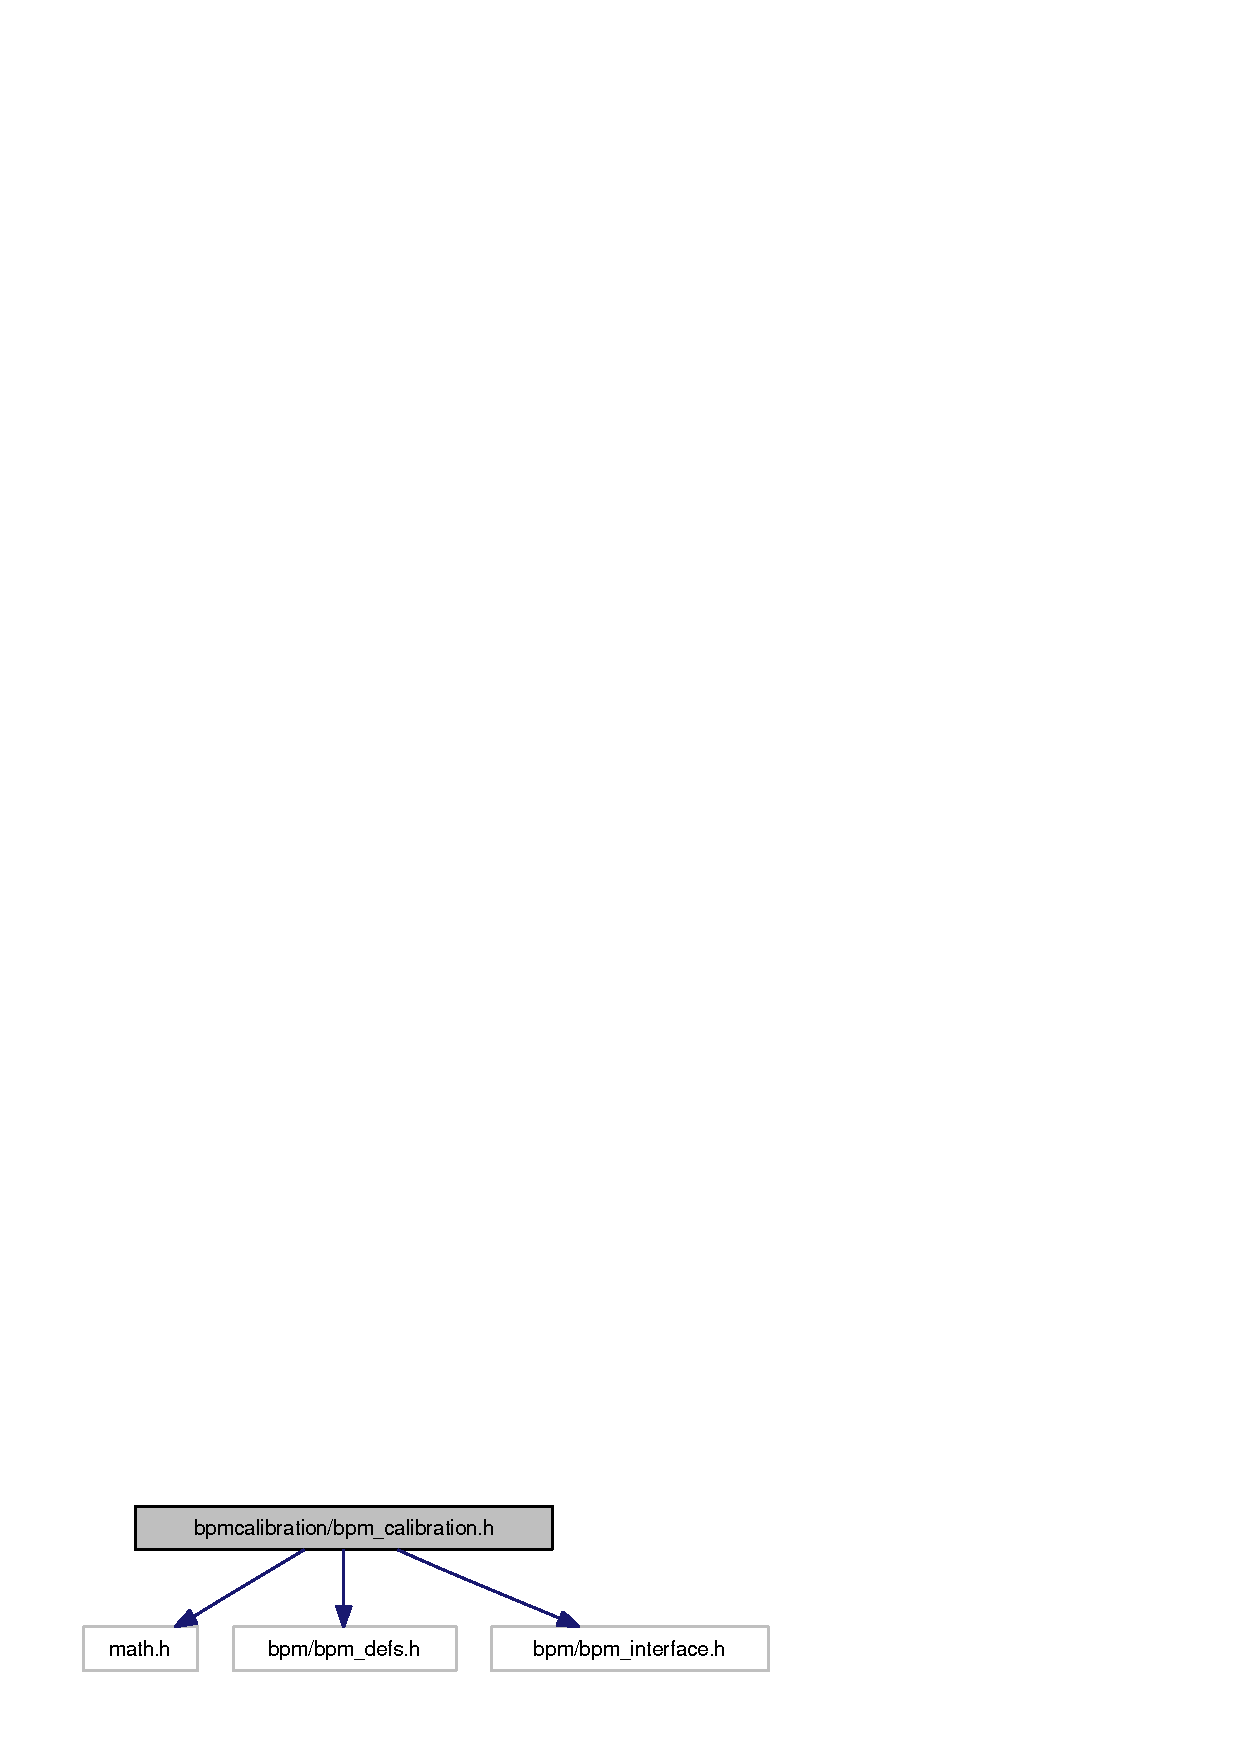
\includegraphics[width=186pt]{bpm__calibration_8h__incl}
\end{center}
\end{figure}
\subsubsection*{Functions}
\begin{CompactItemize}
\item 
EXTERN int {\bf setup\_\-calibration} ({\bf bpmconf\_\-t} $\ast$cnf, {\bf bpmproc\_\-t} $\ast$proc, int npulses, int startpulse, int stoppulse, double angle, double startpos, double endpos, int num\_\-steps, {\bf bunchconf\_\-t} $\ast$bunch)
\item 
EXTERN int {\bf calibrate} ({\bf bpmconf\_\-t} $\ast$bpm, {\bf bunchconf\_\-t} $\ast$bunch, {\bf bpmproc\_\-t} $\ast$proc, int npulses, {\bf bpmcalib\_\-t} $\ast$cal)
\end{CompactItemize}

\subsection{bpmcalibration/calibrate.c File Reference}
\label{calibrate_8c}\index{bpmcalibration/calibrate.c@{bpmcalibration/calibrate.c}}


\subsubsection{Detailed Description}


Definition in file {\bf calibrate.c}.

{\tt \#include $<$bpm/bpm\_\-messages.h$>$}\par
{\tt \#include $<$bpm/bpm\_\-calibration.h$>$}\par
{\tt \#include $<$bpm/bpm\_\-nr.h$>$}\par


Include dependency graph for calibrate.c:\nopagebreak
\begin{figure}[H]
\begin{center}
\leavevmode
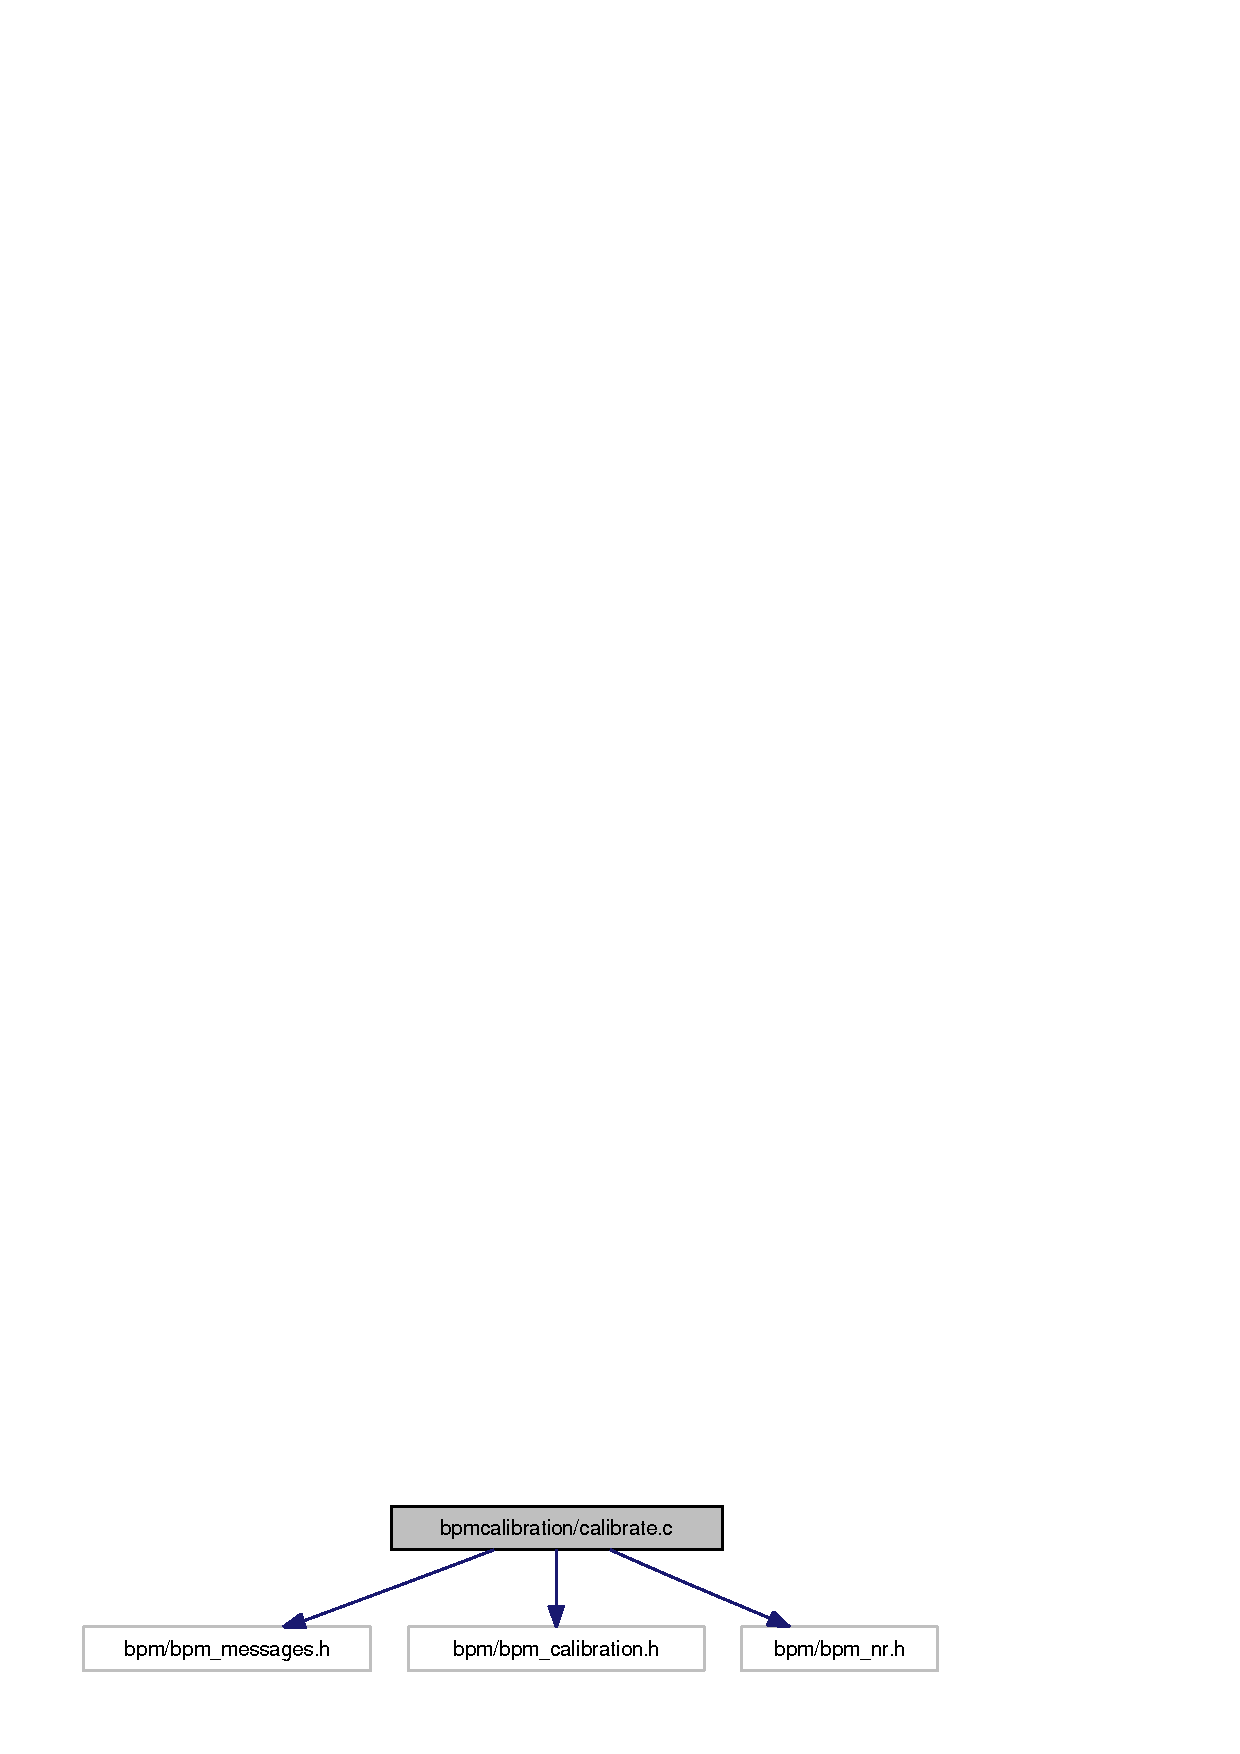
\includegraphics[width=227pt]{calibrate_8c__incl}
\end{center}
\end{figure}
\subsubsection*{Functions}
\begin{CompactItemize}
\item 
int {\bf calibrate} ({\bf bpmconf\_\-t} $\ast$bpm, {\bf bunchconf\_\-t} $\ast$bunch, {\bf bpmproc\_\-t} $\ast$proc, int npulses, {\bf bpmcalib\_\-t} $\ast$cal)
\end{CompactItemize}

\subsection{bpmcalibration/setup\_\-calibration.c File Reference}
\label{setup__calibration_8c}\index{bpmcalibration/setup\_\-calibration.c@{bpmcalibration/setup\_\-calibration.c}}


\subsubsection{Detailed Description}


Definition in file {\bf setup\_\-calibration.c}.

{\tt \#include $<$bpm/bpm\_\-messages.h$>$}\par
{\tt \#include $<$bpm/bpm\_\-calibration.h$>$}\par


Include dependency graph for setup\_\-calibration.c:\nopagebreak
\begin{figure}[H]
\begin{center}
\leavevmode
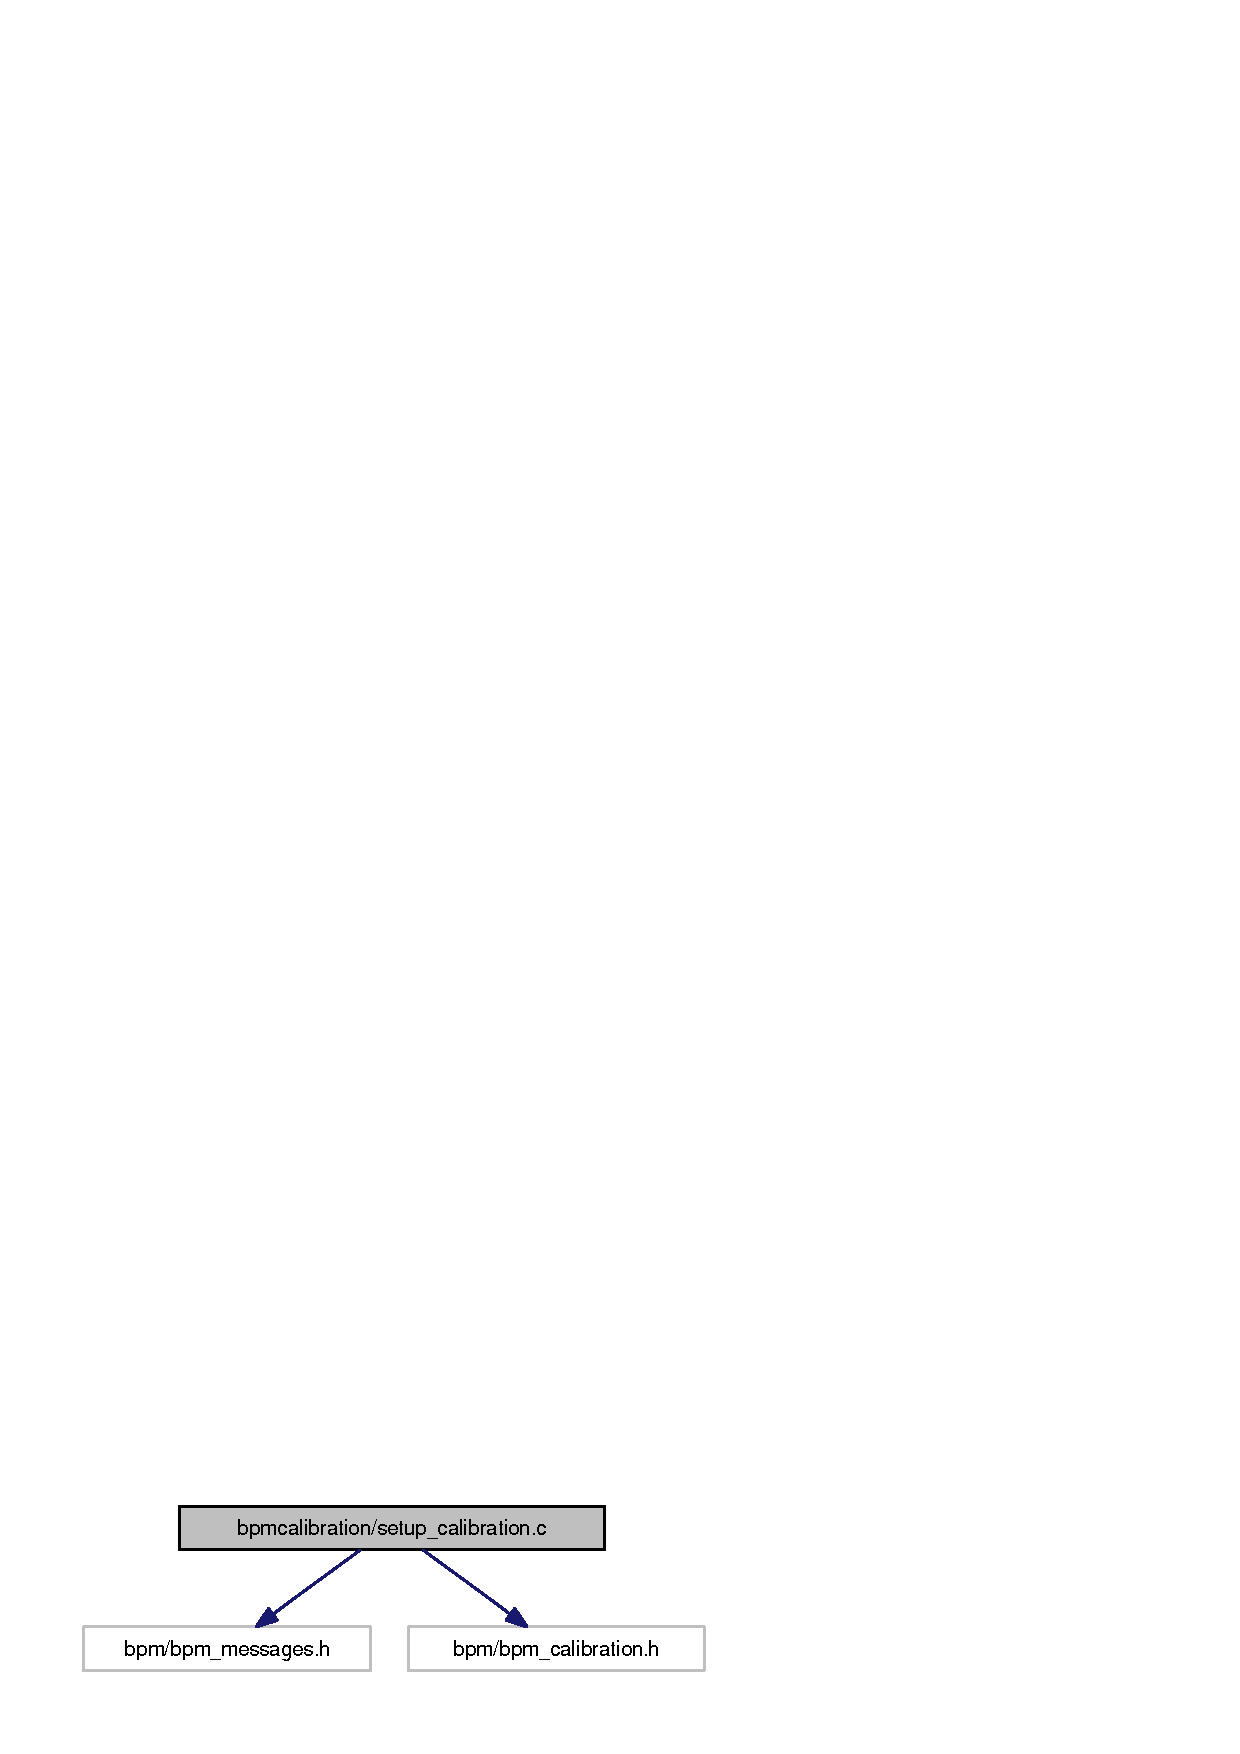
\includegraphics[width=171pt]{setup__calibration_8c__incl}
\end{center}
\end{figure}
\subsubsection*{Functions}
\begin{CompactItemize}
\item 
int {\bf setup\_\-calibration} ({\bf bpmconf\_\-t} $\ast$cnf, {\bf bpmproc\_\-t} $\ast$proc, int npulses, int startpulse, int stoppulse, double angle, double startpos, double endpos, int num\_\-steps, {\bf bunchconf\_\-t} $\ast$bunch)
\end{CompactItemize}

\subsection{bpmdsp/bpm\_\-dsp.h File Reference}
\label{bpm__dsp_8h}\index{bpmdsp/bpm\_\-dsp.h@{bpmdsp/bpm\_\-dsp.h}}


\subsubsection{Detailed Description}
libbpm digital signal processing routines 



Definition in file {\bf bpm\_\-dsp.h}.

{\tt \#include $<$stdio.h$>$}\par
{\tt \#include $<$stdlib.h$>$}\par
{\tt \#include $<$string.h$>$}\par
{\tt \#include $<$math.h$>$}\par
{\tt \#include \char`\"{}bpm/bpm\_\-defs.h\char`\"{}}\par
{\tt \#include \char`\"{}bpm/bpm\_\-messages.h\char`\"{}}\par
{\tt \#include \char`\"{}bpm/bpm\_\-nr.h\char`\"{}}\par
{\tt \#include \char`\"{}bpm/bpm\_\-wf.h\char`\"{}}\par


Include dependency graph for bpm\_\-dsp.h:\nopagebreak
\begin{figure}[H]
\begin{center}
\leavevmode
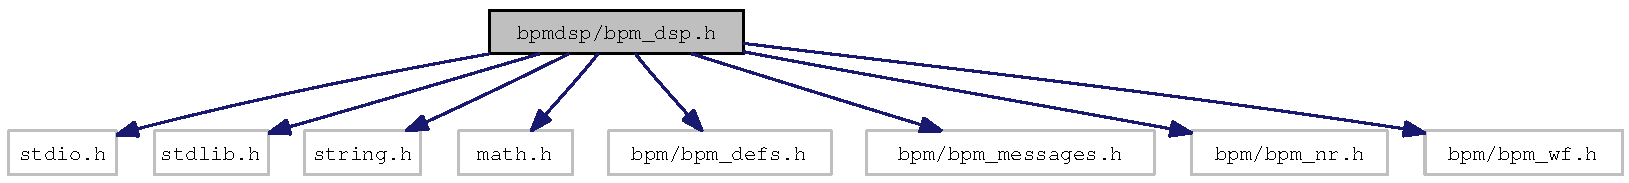
\includegraphics[width=409pt]{bpm__dsp_8h__incl}
\end{center}
\end{figure}


This graph shows which files directly or indirectly include this file:\nopagebreak
\begin{figure}[H]
\begin{center}
\leavevmode
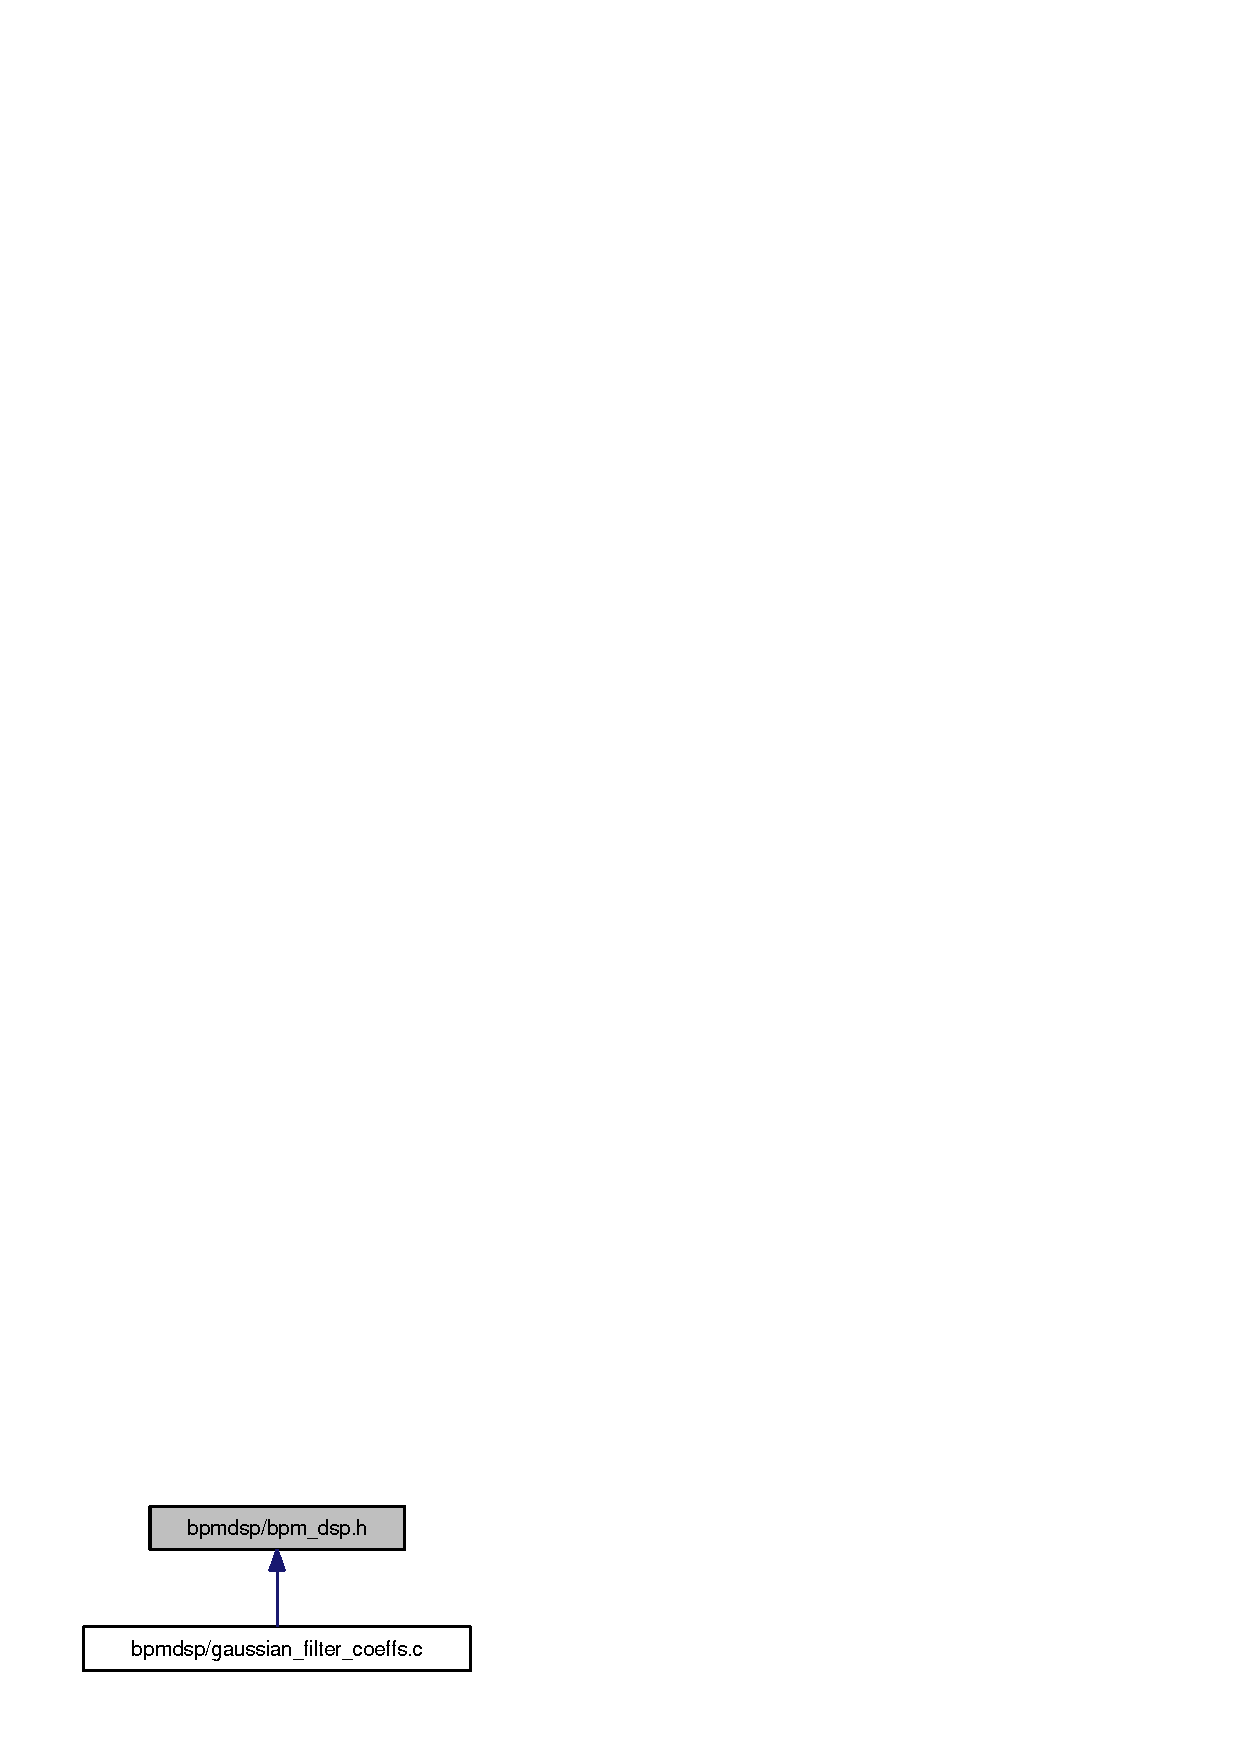
\includegraphics[width=115pt]{bpm__dsp_8h__dep__incl}
\end{center}
\end{figure}
\subsubsection*{Data Structures}
\begin{CompactItemize}
\item 
struct {\bf filterrep\_\-t}
\item 
struct {\bf filter\_\-t}
\end{CompactItemize}
\subsubsection*{Defines}
\begin{CompactItemize}
\item 
\#define {\bf BESSEL}
\item 
\#define {\bf BUTTERWORTH}
\item 
\#define {\bf CHEBYSHEV}
\item 
\#define {\bf RAISEDCOSINE}
\item 
\#define {\bf RESONATOR}
\item 
\#define {\bf GAUSSIAN}
\item 
\#define {\bf BILINEAR\_\-Z\_\-TRANSFORM}
\item 
\#define {\bf MATCHED\_\-Z\_\-TRANSFORM}
\item 
\#define {\bf NO\_\-PREWARP}
\item 
\#define {\bf CAUSAL}
\item 
\#define {\bf ANTICAUSAL}
\item 
\#define {\bf NONCAUSAL}
\item 
\#define {\bf GAUSSIAN\_\-SIGMA\_\-BW}
\item 
\#define {\bf LOWPASS}
\item 
\#define {\bf HIGHPASS}
\item 
\#define {\bf BANDPASS}
\item 
\#define {\bf BANDSTOP}
\item 
\#define {\bf NOTCH}
\item 
\#define {\bf ALLPASS}
\item 
\#define {\bf FIR}
\item 
\#define {\bf IIR}
\item 
\#define {\bf MAXORDER}
\item 
\#define {\bf MAXPZ}
\item 
\#define {\bf FILT\_\-EPS}
\item 
\#define {\bf MAX\_\-RESONATOR\_\-ITER}
\item 
\#define {\bf FFT\_\-FORWARD}
\item 
\#define {\bf FFT\_\-BACKWARD}
\end{CompactItemize}
\subsubsection*{Functions}
\begin{CompactItemize}
\item 
EXTERN {\bf filter\_\-t} $\ast$ {\bf create\_\-filter} (char name[$\,$], unsigned int options, int order, int ns, double fs, double f1, double f2, double par)
\item 
EXTERN int {\bf apply\_\-filter} ({\bf filter\_\-t} $\ast$f, {\bf doublewf\_\-t} $\ast$w)
\item 
EXTERN void {\bf print\_\-filter} (FILE $\ast$of, {\bf filter\_\-t} $\ast$f)
\item 
EXTERN void {\bf delete\_\-filter} ({\bf filter\_\-t} $\ast$f)
\item 
EXTERN int {\bf filter\_\-step\_\-response} ({\bf filter\_\-t} $\ast$f, {\bf doublewf\_\-t} $\ast$w, int itrig)
\item 
EXTERN int {\bf filter\_\-impulse\_\-response} ({\bf filter\_\-t} $\ast$f, {\bf doublewf\_\-t} $\ast$w, int itrig)
\item 
EXTERN {\bf filterrep\_\-t} $\ast$ {\bf create\_\-splane\_\-representation} ({\bf filter\_\-t} $\ast$f)
\item 
EXTERN {\bf filterrep\_\-t} $\ast$ {\bf create\_\-resonator\_\-representation} ({\bf filter\_\-t} $\ast$f)
\item 
EXTERN {\bf filterrep\_\-t} $\ast$ {\bf zplane\_\-transform} ({\bf filter\_\-t} $\ast$f, {\bf filterrep\_\-t} $\ast$s)
\item 
EXTERN void {\bf print\_\-filter\_\-representation} (FILE $\ast$of, {\bf filterrep\_\-t} $\ast$r)
\item 
EXTERN int {\bf normalise\_\-filter} ({\bf filter\_\-t} $\ast$f, {\bf filterrep\_\-t} $\ast$s)
\item 
EXTERN int {\bf calculate\_\-filter\_\-coefficients} ({\bf filter\_\-t} $\ast$f)
\item 
EXTERN int {\bf gaussian\_\-filter\_\-coeffs} ({\bf filter\_\-t} $\ast$f)
\item 
EXTERN int {\bf \_\-expand\_\-complex\_\-polynomial} ({\bf complex\_\-t} $\ast$w, int n, {\bf complex\_\-t} $\ast$a)
\item 
EXTERN {\bf complex\_\-t} {\bf \_\-eval\_\-complex\_\-polynomial} ({\bf complex\_\-t} $\ast$a, int n, {\bf complex\_\-t} z)
\item 
EXTERN int {\bf ddc\_\-initialise} (int ns, double fs)
\item 
EXTERN void {\bf ddc\_\-cleanup} (void)
\item 
int {\bf ddc} ({\bf doublewf\_\-t} $\ast$w, double f, {\bf filter\_\-t} $\ast$filter, {\bf complexwf\_\-t} $\ast$dcw, {\bf doublewf\_\-t} $\ast$bufre, {\bf doublewf\_\-t} $\ast$bufim)
\item 
EXTERN int {\bf fft\_\-gen\_\-tables} (void)
\item 
EXTERN int {\bf fft\_\-initialise} (int ns)
\item 
EXTERN void {\bf fft\_\-cleanup} (void)
\item 
EXTERN int {\bf complexfft} ({\bf complexwf\_\-t} $\ast$z, int fft\_\-mode)
\item 
EXTERN int {\bf realfft} ({\bf doublewf\_\-t} $\ast$y, int fft\_\-mode, {\bf complexwf\_\-t} $\ast$z)
\item 
EXTERN void {\bf norm\_\-phase} (double $\ast$phase)
\end{CompactItemize}

\subsection{bpmdsp/calculate\_\-filter\_\-coefficients.c File Reference}
\label{calculate__filter__coefficients_8c}\index{bpmdsp/calculate\_\-filter\_\-coefficients.c@{bpmdsp/calculate\_\-filter\_\-coefficients.c}}


\subsubsection{Detailed Description}


Definition in file {\bf calculate\_\-filter\_\-coefficients.c}.

{\tt \#include \char`\"{}bpm/bpm\_\-dsp.h\char`\"{}}\par


Include dependency graph for calculate\_\-filter\_\-coefficients.c:\nopagebreak
\begin{figure}[H]
\begin{center}
\leavevmode
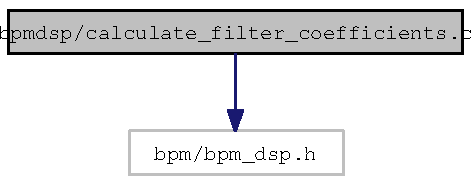
\includegraphics[width=131pt]{calculate__filter__coefficients_8c__incl}
\end{center}
\end{figure}
\subsubsection*{Functions}
\begin{CompactItemize}
\item 
int {\bf \_\-expand\_\-complex\_\-polynomial} ({\bf complex\_\-t} $\ast$w, int n, {\bf complex\_\-t} $\ast$a)
\item 
{\bf complex\_\-t} {\bf \_\-eval\_\-complex\_\-polynomial} ({\bf complex\_\-t} $\ast$a, int n, {\bf complex\_\-t} z)
\item 
int {\bf calculate\_\-filter\_\-coefficients} ({\bf filter\_\-t} $\ast$f)
\end{CompactItemize}

\subsection{bpmdsp/create\_\-filter.c File Reference}
\label{create__filter_8c}\index{bpmdsp/create\_\-filter.c@{bpmdsp/create\_\-filter.c}}


\subsubsection{Detailed Description}


Definition in file {\bf create\_\-filter.c}.

{\tt \#include $<$string.h$>$}\par
{\tt \#include $<$stdlib.h$>$}\par
{\tt \#include \char`\"{}bpm/bpm\_\-dsp.h\char`\"{}}\par


Include dependency graph for create\_\-filter.c:\nopagebreak
\begin{figure}[H]
\begin{center}
\leavevmode
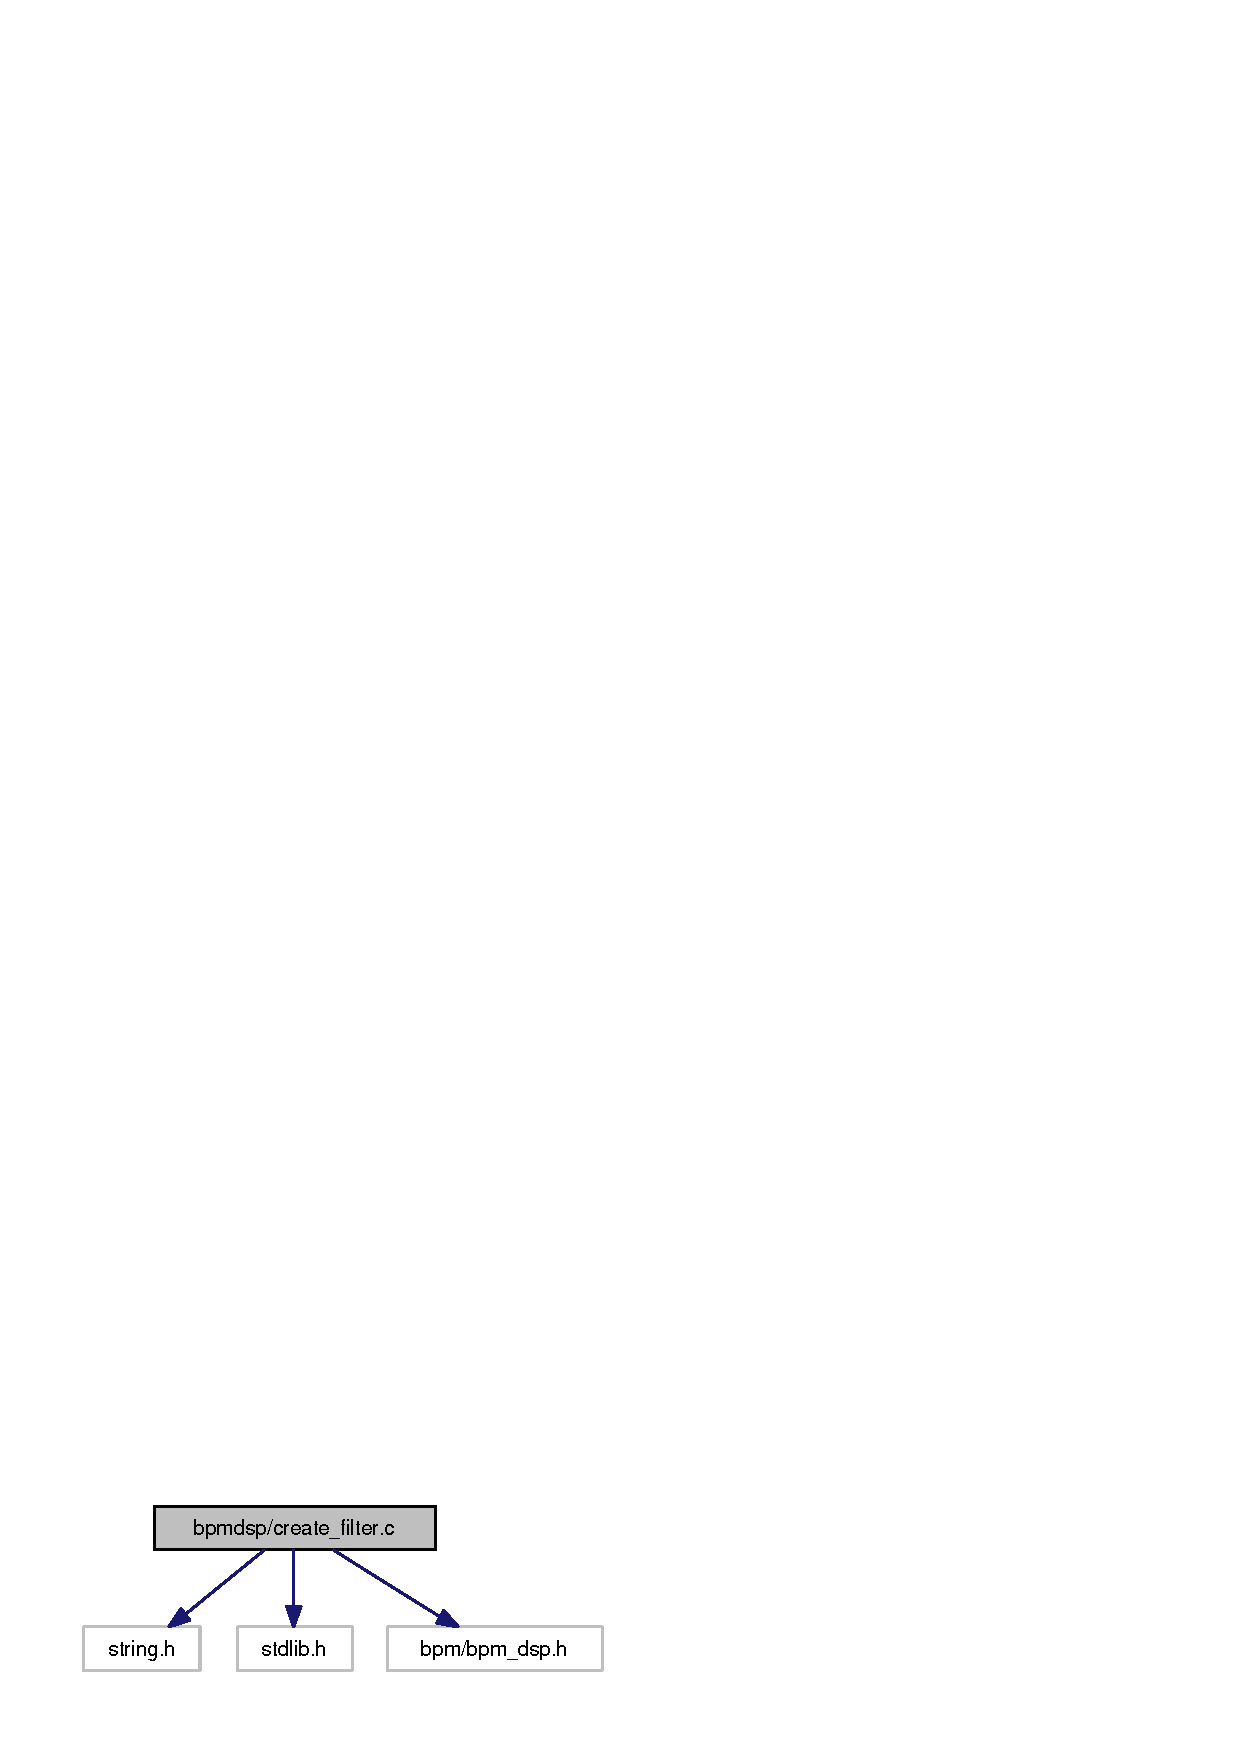
\includegraphics[width=146pt]{create__filter_8c__incl}
\end{center}
\end{figure}
\subsubsection*{Functions}
\begin{CompactItemize}
\item 
{\bf filter\_\-t} $\ast$ {\bf create\_\-filter} (char name[$\,$], unsigned int options, int order, int ns, double fs, double f1, double f2, double par)
\end{CompactItemize}

\subsection{bpmdsp/create\_\-resonator\_\-representation.c File Reference}
\label{create__resonator__representation_8c}\index{bpmdsp/create\_\-resonator\_\-representation.c@{bpmdsp/create\_\-resonator\_\-representation.c}}


\subsubsection{Detailed Description}


Definition in file {\bf create\_\-resonator\_\-representation.c}.

{\tt \#include \char`\"{}bpm/bpm\_\-dsp.h\char`\"{}}\par


Include dependency graph for create\_\-resonator\_\-representation.c:\nopagebreak
\begin{figure}[H]
\begin{center}
\leavevmode
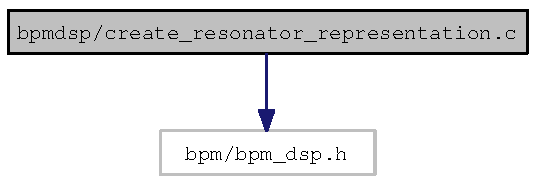
\includegraphics[width=146pt]{create__resonator__representation_8c__incl}
\end{center}
\end{figure}
\subsubsection*{Functions}
\begin{CompactItemize}
\item 
{\bf complex\_\-t} \textbf{\_\-reflect} ({\bf complex\_\-t} z)\label{create__resonator__representation_8c_5f5822799f26a42df071d1662eaafb19}

\item 
{\bf filterrep\_\-t} $\ast$ {\bf create\_\-resonator\_\-representation} ({\bf filter\_\-t} $\ast$f)
\end{CompactItemize}

\subsection{bpmdsp/create\_\-splane\_\-representation.c File Reference}
\label{create__splane__representation_8c}\index{bpmdsp/create\_\-splane\_\-representation.c@{bpmdsp/create\_\-splane\_\-representation.c}}


\subsubsection{Detailed Description}


Definition in file {\bf create\_\-splane\_\-representation.c}.

{\tt \#include \char`\"{}bpm/bpm\_\-dsp.h\char`\"{}}\par


Include dependency graph for create\_\-splane\_\-representation.c:\nopagebreak
\begin{figure}[H]
\begin{center}
\leavevmode
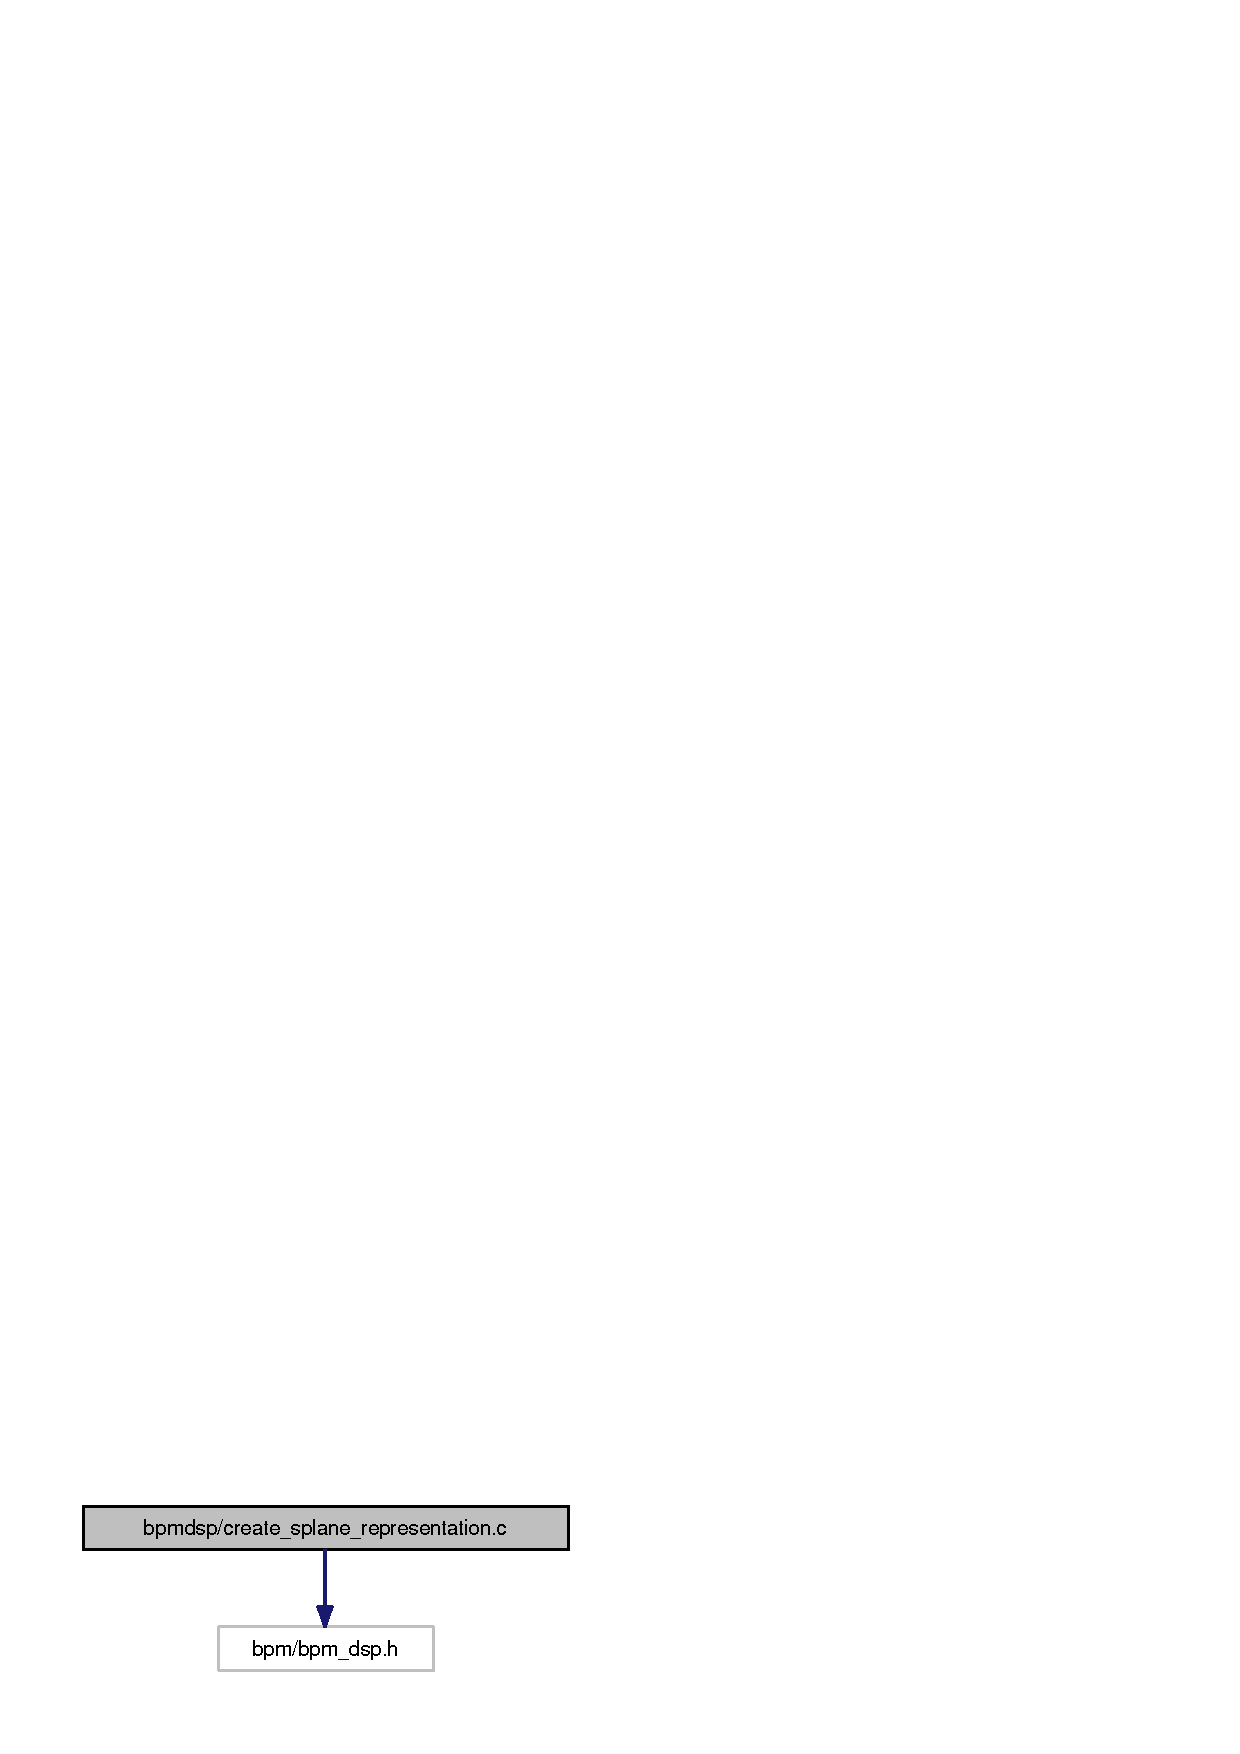
\includegraphics[width=138pt]{create__splane__representation_8c__incl}
\end{center}
\end{figure}
\subsubsection*{Functions}
\begin{CompactItemize}
\item 
void \textbf{\_\-add\_\-splane\_\-pole} ({\bf filterrep\_\-t} $\ast$r, {\bf complex\_\-t} z)\label{create__splane__representation_8c_4350e23bc8b050bf533531a9c5000b7b}

\item 
{\bf filterrep\_\-t} $\ast$ {\bf create\_\-splane\_\-representation} ({\bf filter\_\-t} $\ast$f)
\end{CompactItemize}

\subsection{bpmdsp/ddc.c File Reference}
\label{ddc_8c}\index{bpmdsp/ddc.c@{bpmdsp/ddc.c}}


\subsubsection{Detailed Description}


Definition in file {\bf ddc.c}.

{\tt \#include \char`\"{}bpm/bpm\_\-dsp.h\char`\"{}}\par


Include dependency graph for ddc.c:\nopagebreak
\begin{figure}[H]
\begin{center}
\leavevmode
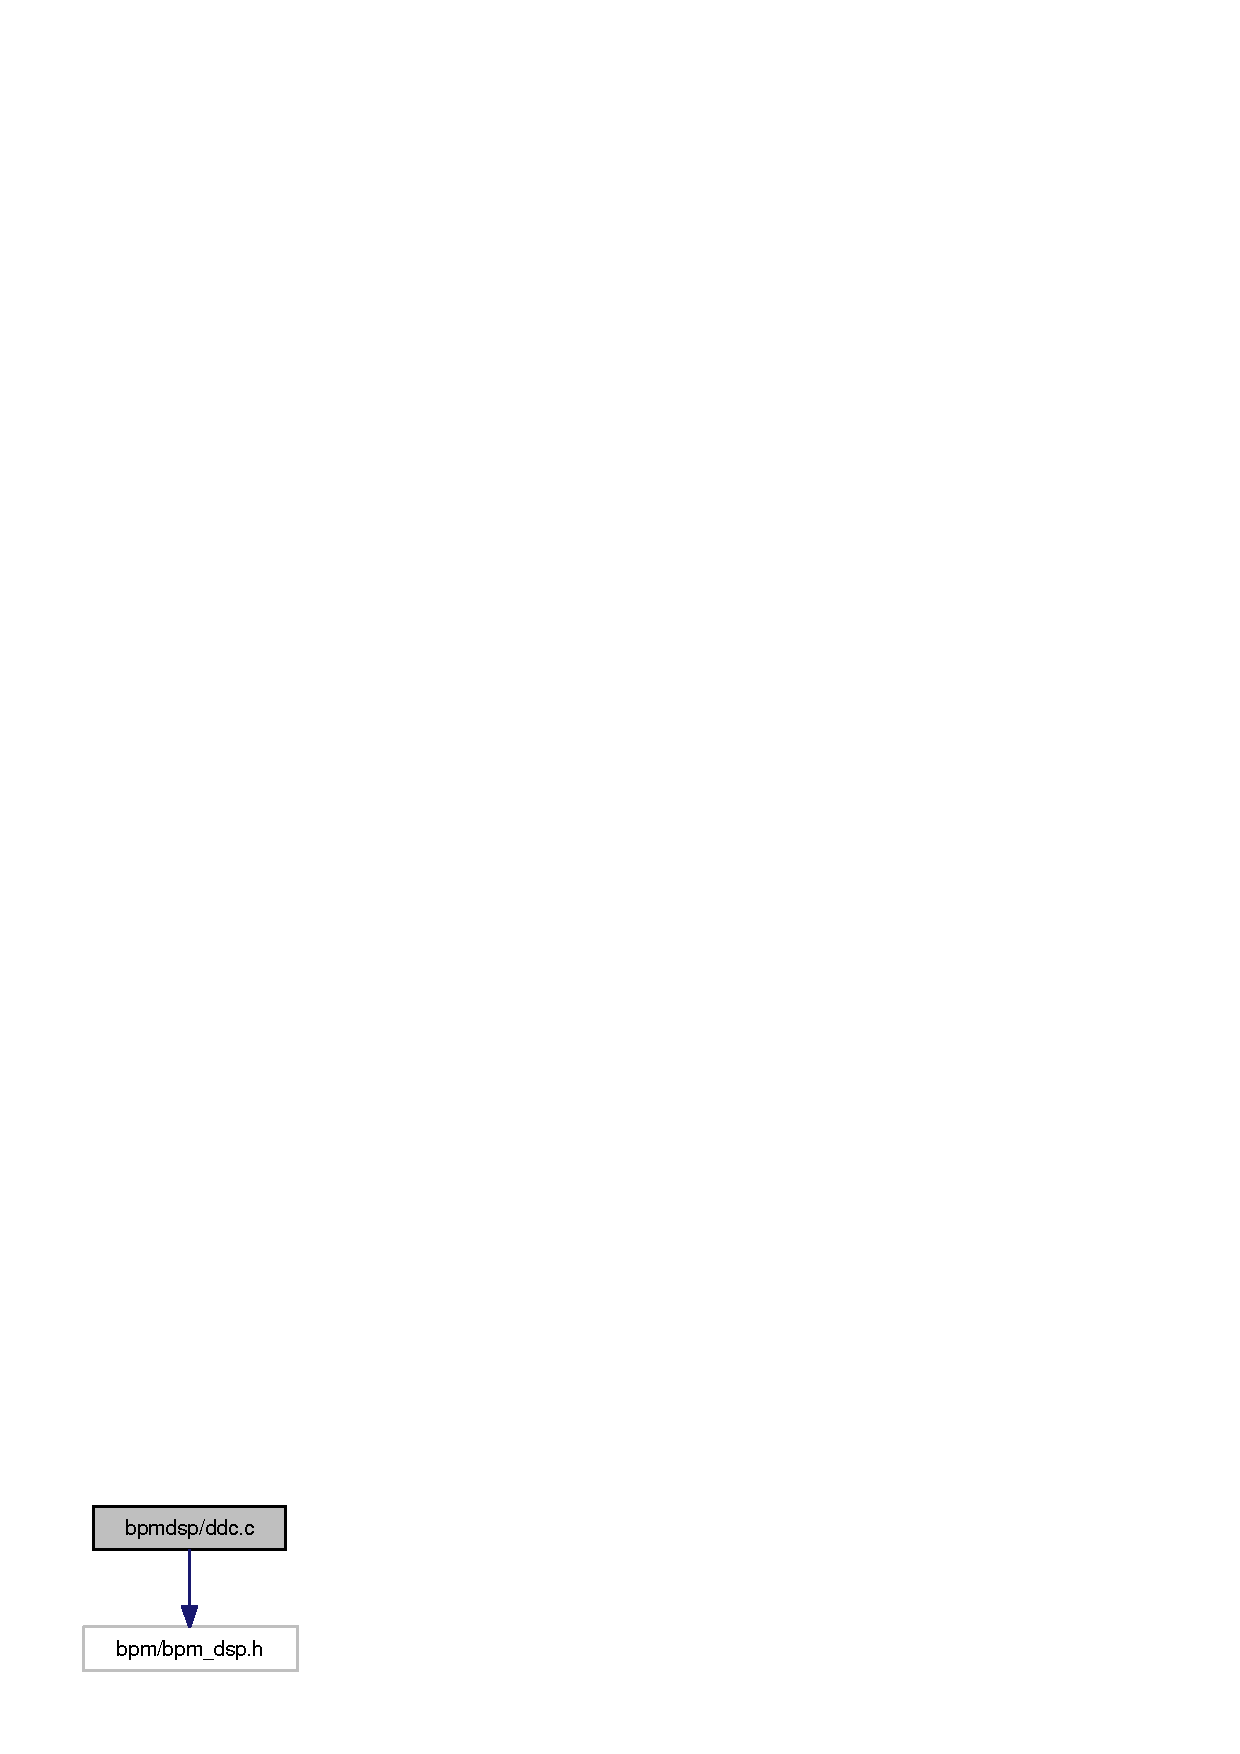
\includegraphics[width=73pt]{ddc_8c__incl}
\end{center}
\end{figure}
\subsubsection*{Functions}
\begin{CompactItemize}
\item 
int \textbf{\_\-check\_\-ddc\_\-buffers} (int ns, double fs)\label{ddc_8c_f331a899b22b7631f27b5835ac6379f0}

\item 
int {\bf ddc\_\-initialise} (int ns, double fs)
\item 
void {\bf ddc\_\-cleanup} (void)
\item 
int {\bf ddc} ({\bf doublewf\_\-t} $\ast$w, double f, {\bf filter\_\-t} $\ast$filter, {\bf complexwf\_\-t} $\ast$dcw, {\bf doublewf\_\-t} $\ast$bufre, {\bf doublewf\_\-t} $\ast$bufim)
\end{CompactItemize}

\subsection{bpmdsp/delete\_\-filter.c File Reference}
\label{delete__filter_8c}\index{bpmdsp/delete\_\-filter.c@{bpmdsp/delete\_\-filter.c}}


\subsubsection{Detailed Description}


Definition in file {\bf delete\_\-filter.c}.

{\tt \#include \char`\"{}bpm/bpm\_\-dsp.h\char`\"{}}\par


Include dependency graph for delete\_\-filter.c:\nopagebreak
\begin{figure}[H]
\begin{center}
\leavevmode
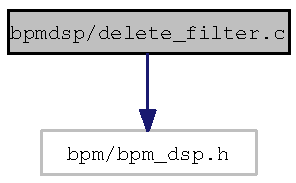
\includegraphics[width=89pt]{delete__filter_8c__incl}
\end{center}
\end{figure}
\subsubsection*{Functions}
\begin{CompactItemize}
\item 
void {\bf delete\_\-filter} ({\bf filter\_\-t} $\ast$f)
\end{CompactItemize}

\subsection{bpmdsp/discrete\_\-fourier\_\-transforms.c File Reference}
\label{discrete__fourier__transforms_8c}\index{bpmdsp/discrete\_\-fourier\_\-transforms.c@{bpmdsp/discrete\_\-fourier\_\-transforms.c}}


\subsubsection{Detailed Description}


Definition in file {\bf discrete\_\-fourier\_\-transforms.c}.

{\tt \#include \char`\"{}bpm/bpm\_\-wf.h\char`\"{}}\par
{\tt \#include \char`\"{}bpm/bpm\_\-dsp.h\char`\"{}}\par


Include dependency graph for discrete\_\-fourier\_\-transforms.c:\nopagebreak
\begin{figure}[H]
\begin{center}
\leavevmode
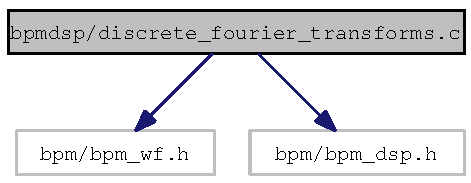
\includegraphics[width=131pt]{discrete__fourier__transforms_8c__incl}
\end{center}
\end{figure}
\subsubsection*{Functions}
\begin{CompactItemize}
\item 
void \textbf{cdft} (int, int, double $\ast$, int $\ast$, double $\ast$)\label{discrete__fourier__transforms_8c_dd439be0f19853cd7568299e4e9f2043}

\item 
void \textbf{rdft} (int, int, double $\ast$, int $\ast$, double $\ast$)\label{discrete__fourier__transforms_8c_39caf6956db3e0243c1a29009d4bf68c}

\item 
int \textbf{\_\-is\_\-pow2} (int n)\label{discrete__fourier__transforms_8c_ae95d6a6ef87ec161047540b4e675fdd}

\item 
int \textbf{\_\-check\_\-fft\_\-buffers} (int ns)\label{discrete__fourier__transforms_8c_fa13ee764b0fe25cf3c4b99e5205bb5d}

\item 
int {\bf fft\_\-gen\_\-tables} (void)
\item 
int {\bf fft\_\-initialise} (int ns)
\item 
void {\bf fft\_\-cleanup} (void)
\item 
int {\bf complexfft} ({\bf complexwf\_\-t} $\ast$z, int fft\_\-mode)
\item 
int {\bf realfft} ({\bf doublewf\_\-t} $\ast$y, int fft\_\-mode, {\bf complexwf\_\-t} $\ast$z)
\end{CompactItemize}

\subsection{bpmdsp/filter\_\-impulse\_\-response.c File Reference}
\label{filter__impulse__response_8c}\index{bpmdsp/filter\_\-impulse\_\-response.c@{bpmdsp/filter\_\-impulse\_\-response.c}}


\subsubsection{Detailed Description}


Definition in file {\bf filter\_\-impulse\_\-response.c}.

{\tt \#include \char`\"{}bpm/bpm\_\-dsp.h\char`\"{}}\par


Include dependency graph for filter\_\-impulse\_\-response.c:\nopagebreak
\begin{figure}[H]
\begin{center}
\leavevmode
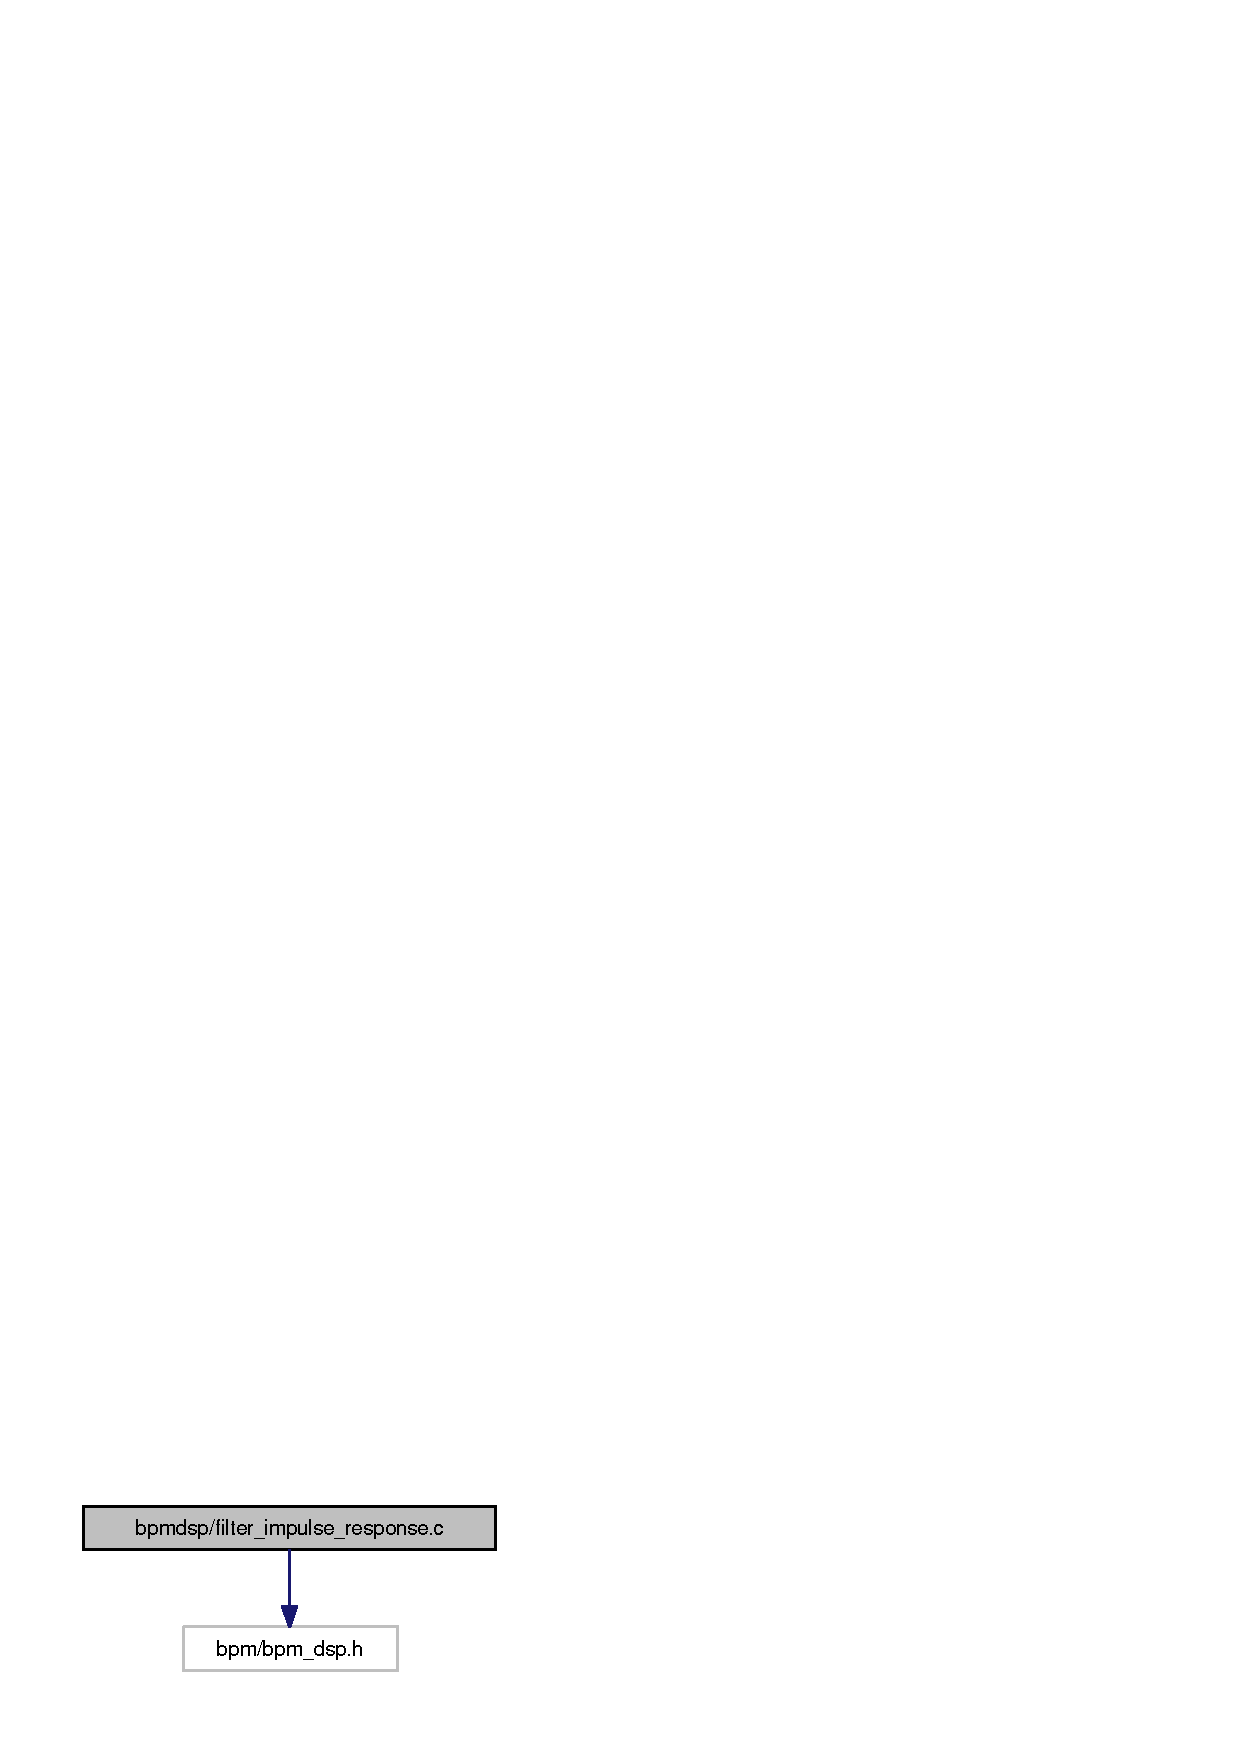
\includegraphics[width=121pt]{filter__impulse__response_8c__incl}
\end{center}
\end{figure}
\subsubsection*{Functions}
\begin{CompactItemize}
\item 
int {\bf filter\_\-impulse\_\-response} ({\bf filter\_\-t} $\ast$f, {\bf doublewf\_\-t} $\ast$w, int itrig)
\end{CompactItemize}

\subsection{bpmdsp/filter\_\-step\_\-response.c File Reference}
\label{filter__step__response_8c}\index{bpmdsp/filter\_\-step\_\-response.c@{bpmdsp/filter\_\-step\_\-response.c}}


\subsubsection{Detailed Description}


Definition in file {\bf filter\_\-step\_\-response.c}.

{\tt \#include \char`\"{}bpm/bpm\_\-dsp.h\char`\"{}}\par


Include dependency graph for filter\_\-step\_\-response.c:\nopagebreak
\begin{figure}[H]
\begin{center}
\leavevmode
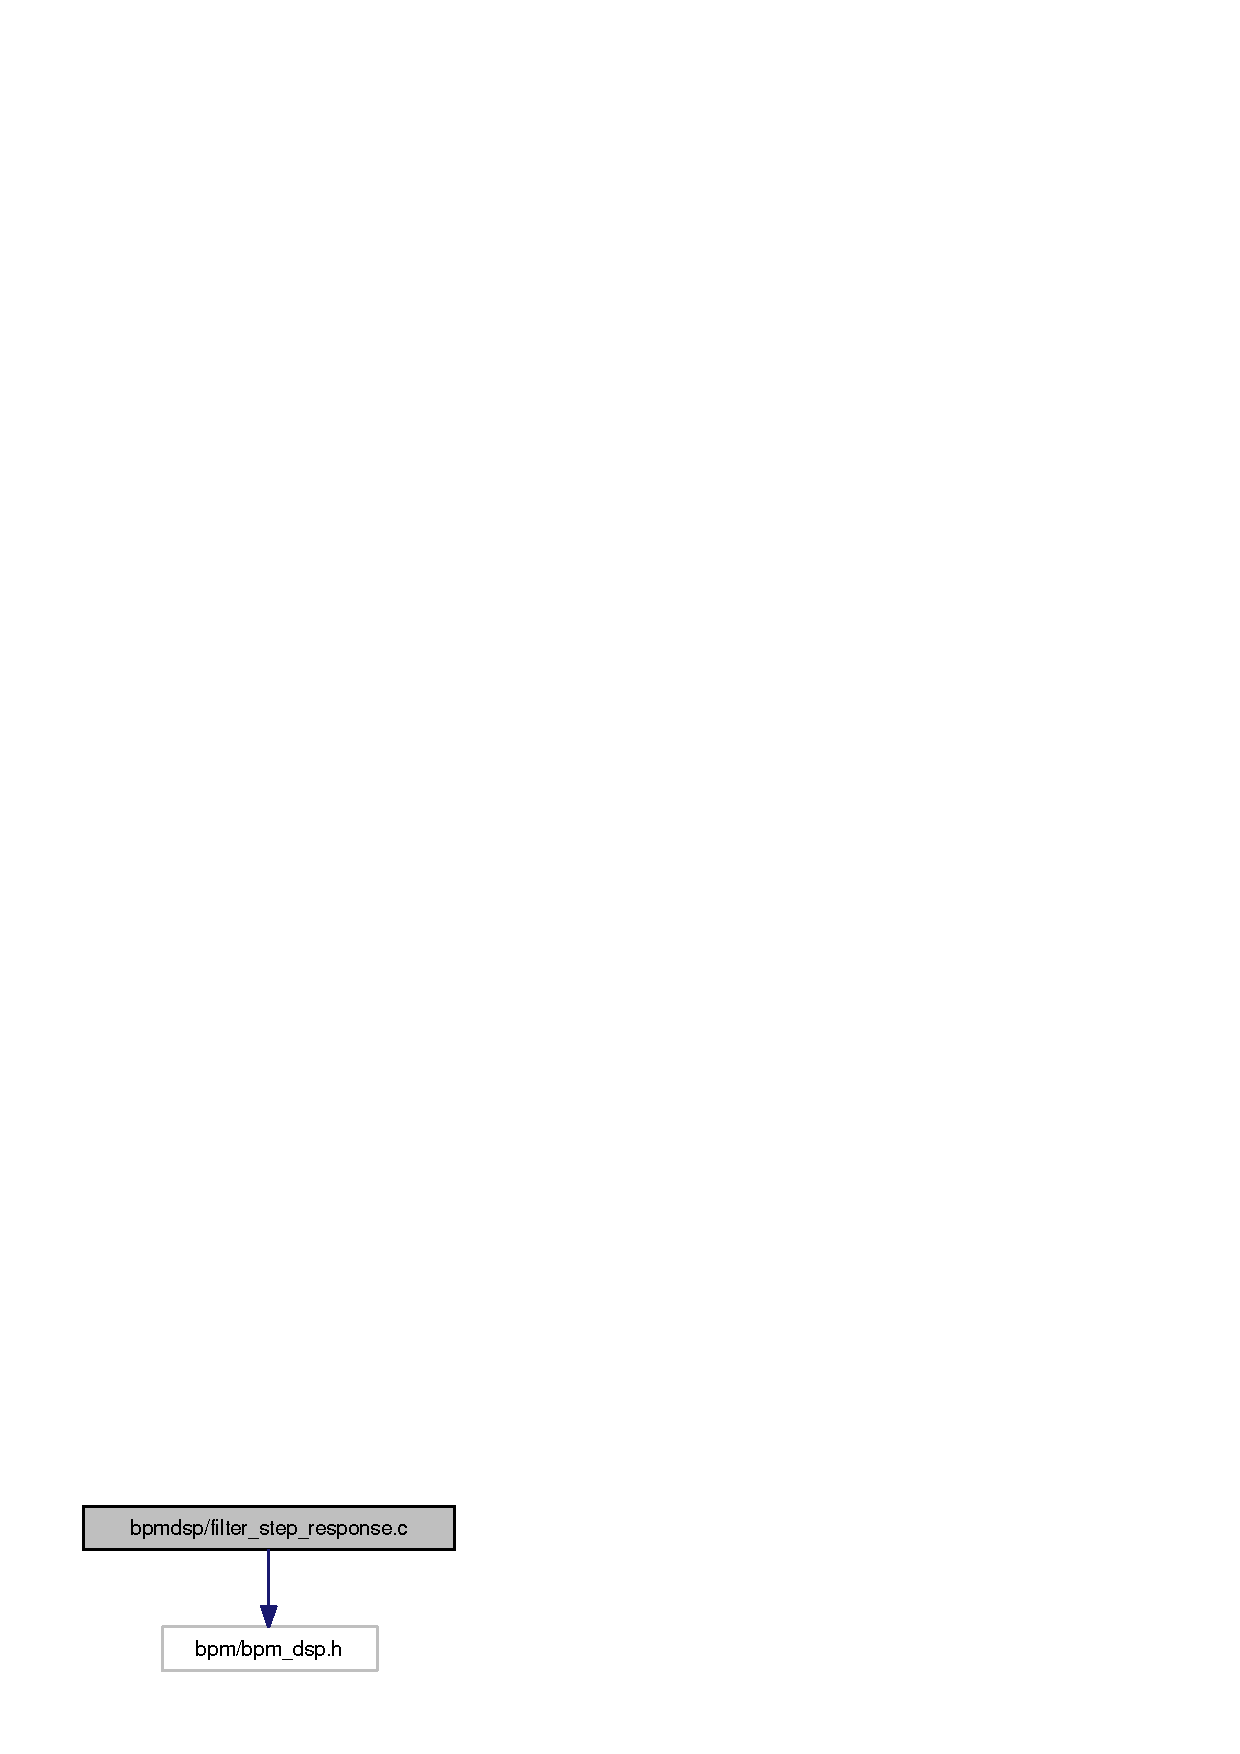
\includegraphics[width=111pt]{filter__step__response_8c__incl}
\end{center}
\end{figure}
\subsubsection*{Functions}
\begin{CompactItemize}
\item 
int {\bf filter\_\-step\_\-response} ({\bf filter\_\-t} $\ast$f, {\bf doublewf\_\-t} $\ast$w, int itrig)
\end{CompactItemize}

\subsection{bpmdsp/gaussian\_\-filter\_\-coeffs.c File Reference}
\label{gaussian__filter__coeffs_8c}\index{bpmdsp/gaussian\_\-filter\_\-coeffs.c@{bpmdsp/gaussian\_\-filter\_\-coeffs.c}}


\subsubsection{Detailed Description}


Definition in file {\bf gaussian\_\-filter\_\-coeffs.c}.

{\tt \#include \char`\"{}bpm\_\-dsp.h\char`\"{}}\par


Include dependency graph for gaussian\_\-filter\_\-coeffs.c:\nopagebreak
\begin{figure}[H]
\begin{center}
\leavevmode
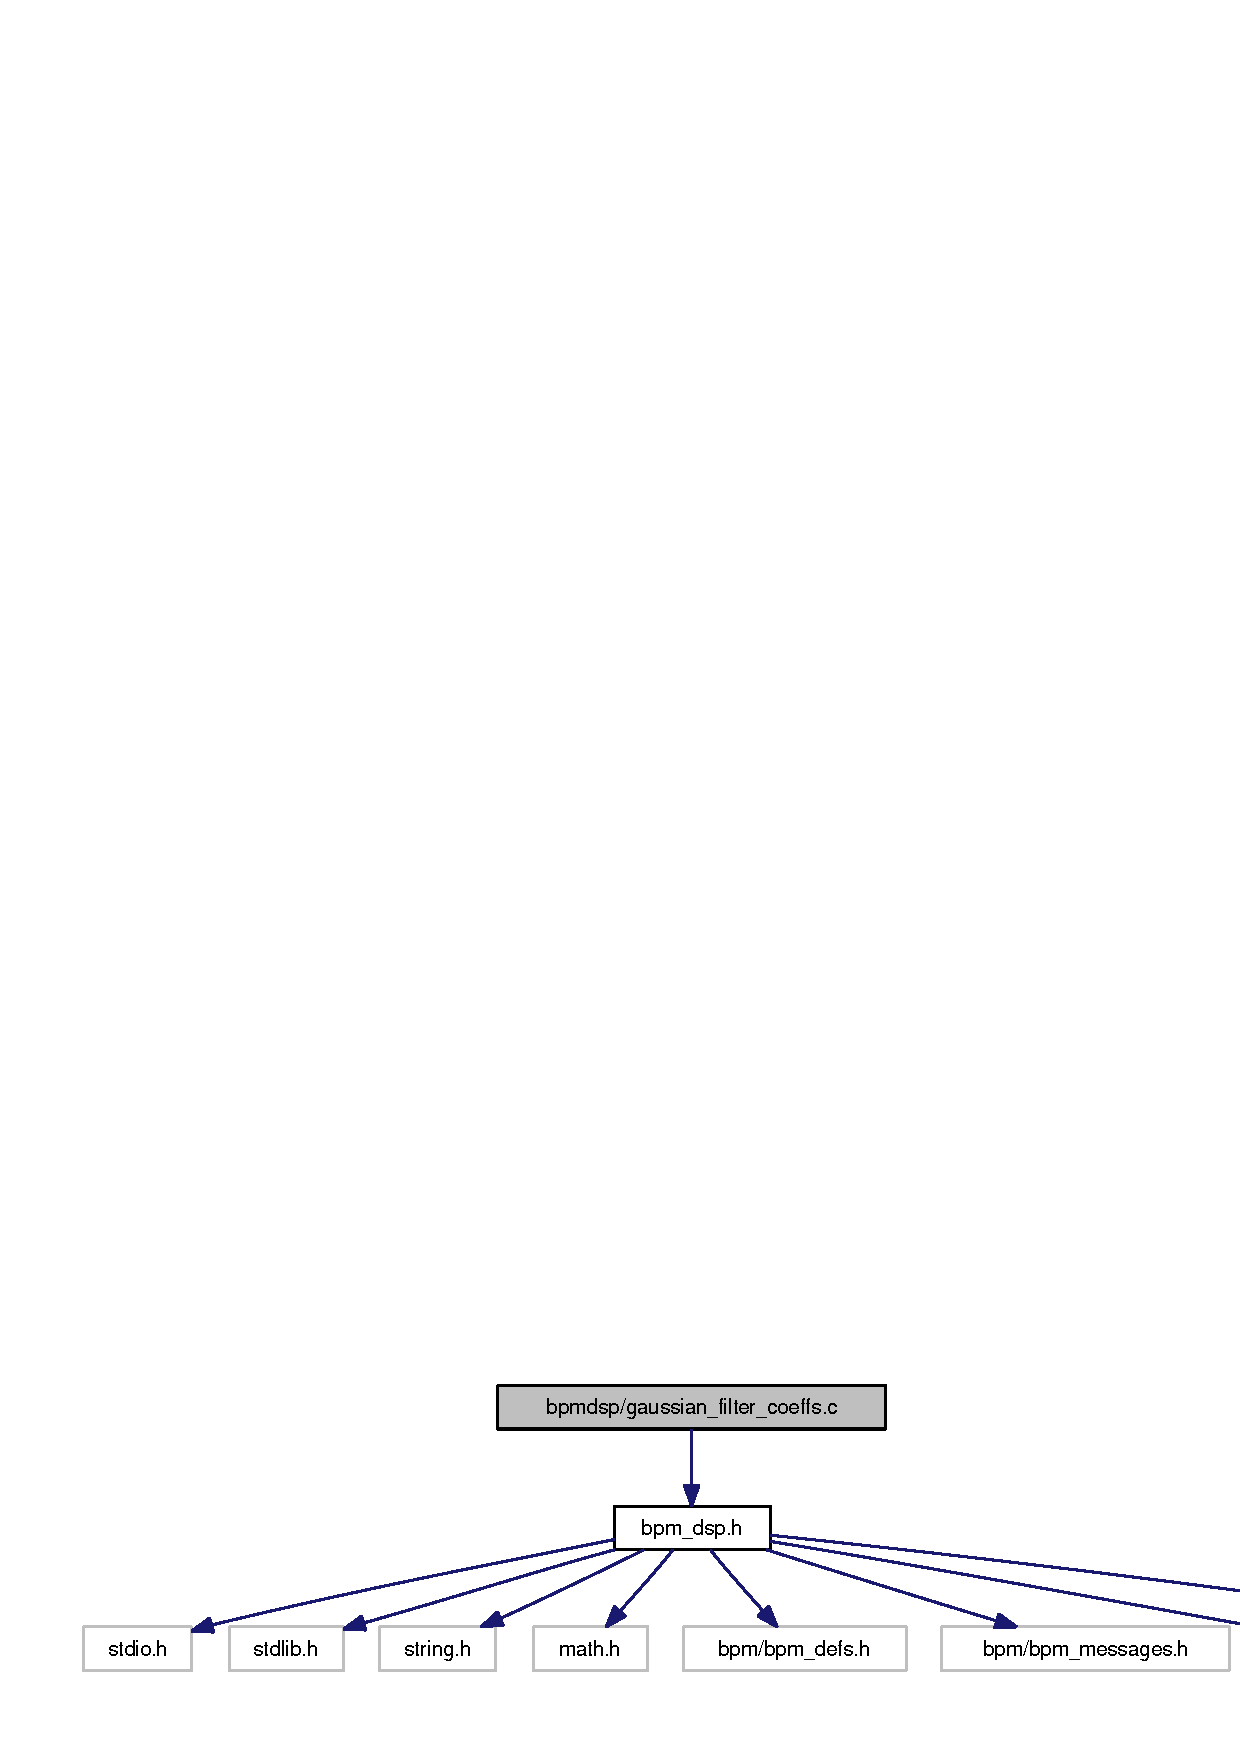
\includegraphics[width=409pt]{gaussian__filter__coeffs_8c__incl}
\end{center}
\end{figure}
\subsubsection*{Functions}
\begin{CompactItemize}
\item 
int {\bf gaussian\_\-filter\_\-coeffs} ({\bf filter\_\-t} $\ast$f)
\end{CompactItemize}

\subsection{bpmdsp/norm\_\-phase.c File Reference}
\label{norm__phase_8c}\index{bpmdsp/norm\_\-phase.c@{bpmdsp/norm\_\-phase.c}}


\subsubsection{Detailed Description}


Definition in file {\bf norm\_\-phase.c}.

{\tt \#include $<$bpm/bpm\_\-dsp.h$>$}\par


Include dependency graph for norm\_\-phase.c:\nopagebreak
\begin{figure}[H]
\begin{center}
\leavevmode
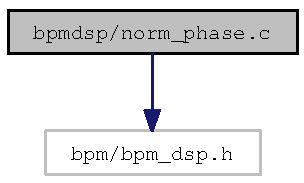
\includegraphics[width=91pt]{norm__phase_8c__incl}
\end{center}
\end{figure}
\subsubsection*{Functions}
\begin{CompactItemize}
\item 
void {\bf norm\_\-phase} (double $\ast$phase)
\end{CompactItemize}

\subsection{bpmdsp/normalise\_\-filter.c File Reference}
\label{normalise__filter_8c}\index{bpmdsp/normalise\_\-filter.c@{bpmdsp/normalise\_\-filter.c}}


\subsubsection{Detailed Description}


Definition in file {\bf normalise\_\-filter.c}.

{\tt \#include \char`\"{}bpm/bpm\_\-dsp.h\char`\"{}}\par


Include dependency graph for normalise\_\-filter.c:\nopagebreak
\begin{figure}[H]
\begin{center}
\leavevmode
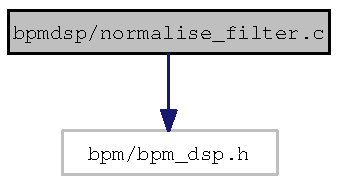
\includegraphics[width=99pt]{normalise__filter_8c__incl}
\end{center}
\end{figure}
\subsubsection*{Functions}
\begin{CompactItemize}
\item 
int {\bf normalise\_\-filter} ({\bf filter\_\-t} $\ast$f, {\bf filterrep\_\-t} $\ast$s)
\end{CompactItemize}

\subsection{bpmdsp/print\_\-filter.c File Reference}
\label{print__filter_8c}\index{bpmdsp/print\_\-filter.c@{bpmdsp/print\_\-filter.c}}


\subsubsection{Detailed Description}


Definition in file {\bf print\_\-filter.c}.

{\tt \#include \char`\"{}bpm/bpm\_\-dsp.h\char`\"{}}\par


Include dependency graph for print\_\-filter.c:\nopagebreak
\begin{figure}[H]
\begin{center}
\leavevmode
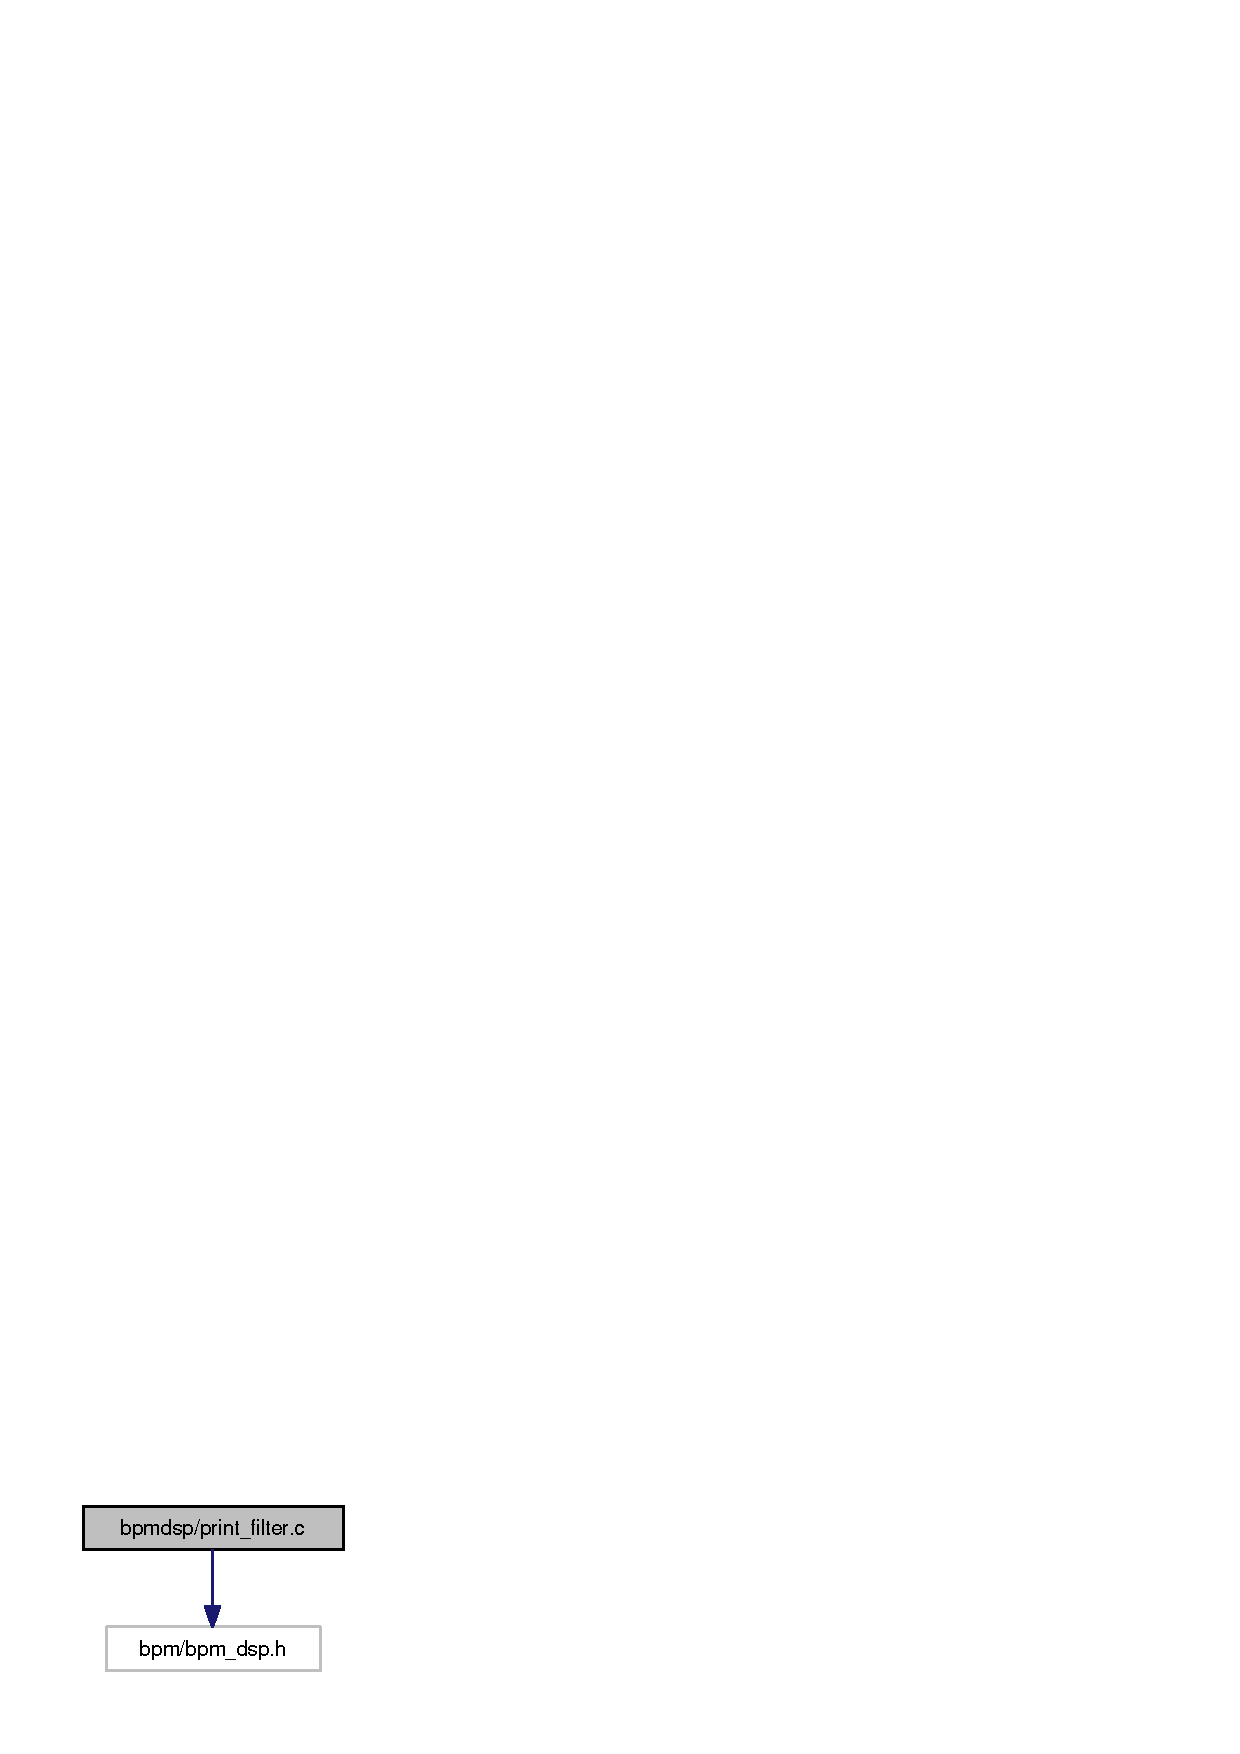
\includegraphics[width=84pt]{print__filter_8c__incl}
\end{center}
\end{figure}
\subsubsection*{Functions}
\begin{CompactItemize}
\item 
void {\bf print\_\-filter} (FILE $\ast$of, {\bf filter\_\-t} $\ast$f)
\end{CompactItemize}

\subsection{bpmdsp/print\_\-filter\_\-representation.c File Reference}
\label{print__filter__representation_8c}\index{bpmdsp/print\_\-filter\_\-representation.c@{bpmdsp/print\_\-filter\_\-representation.c}}


\subsubsection{Detailed Description}


Definition in file {\bf print\_\-filter\_\-representation.c}.

{\tt \#include \char`\"{}bpm/bpm\_\-dsp.h\char`\"{}}\par


Include dependency graph for print\_\-filter\_\-representation.c:\nopagebreak
\begin{figure}[H]
\begin{center}
\leavevmode
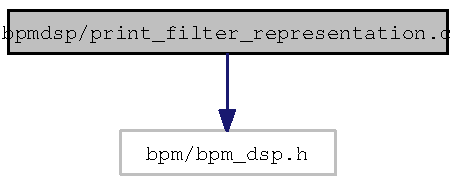
\includegraphics[width=127pt]{print__filter__representation_8c__incl}
\end{center}
\end{figure}
\subsubsection*{Functions}
\begin{CompactItemize}
\item 
void {\bf print\_\-filter\_\-representation} (FILE $\ast$of, {\bf filterrep\_\-t} $\ast$r)
\end{CompactItemize}

\subsection{bpmdsp/zplane\_\-transform.c File Reference}
\label{zplane__transform_8c}\index{bpmdsp/zplane\_\-transform.c@{bpmdsp/zplane\_\-transform.c}}


\subsubsection{Detailed Description}


Definition in file {\bf zplane\_\-transform.c}.

{\tt \#include \char`\"{}bpm/bpm\_\-dsp.h\char`\"{}}\par


Include dependency graph for zplane\_\-transform.c:\nopagebreak
\begin{figure}[H]
\begin{center}
\leavevmode
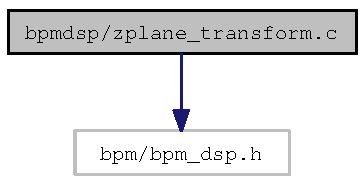
\includegraphics[width=105pt]{zplane__transform_8c__incl}
\end{center}
\end{figure}
\subsubsection*{Functions}
\begin{CompactItemize}
\item 
{\bf filterrep\_\-t} $\ast$ {\bf zplane\_\-transform} ({\bf filter\_\-t} $\ast$f, {\bf filterrep\_\-t} $\ast$s)
\end{CompactItemize}

\subsection{bpminterface/bpm\_\-interface.h File Reference}
\label{bpm__interface_8h}\index{bpminterface/bpm\_\-interface.h@{bpminterface/bpm\_\-interface.h}}


\subsubsection{Detailed Description}
Front end interface structure definitions and handlers. 

This header contains the front-end interface structures and handlers for libbpm. They define a set of user friendly structures like bpmconf\_\-t, bpmcalib\_\-t, beamconf\_\-t etc... to work with the bpm data. 

Definition in file {\bf bpm\_\-interface.h}.

{\tt \#include $<$stdio.h$>$}\par
{\tt \#include $<$stdlib.h$>$}\par
{\tt \#include $<$string.h$>$}\par
{\tt \#include $<$bpm/bpm\_\-defs.h$>$}\par
{\tt \#include $<$bpm/bpm\_\-wf.h$>$}\par
{\tt \#include $<$bpm/bpm\_\-dsp.h$>$}\par


Include dependency graph for bpm\_\-interface.h:\nopagebreak
\begin{figure}[H]
\begin{center}
\leavevmode
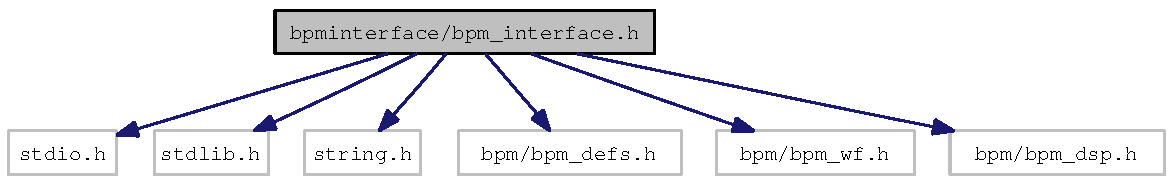
\includegraphics[width=299pt]{bpm__interface_8h__incl}
\end{center}
\end{figure}
\subsubsection*{Data Structures}
\begin{CompactItemize}
\item 
struct {\bf bpmconf}
\item 
struct {\bf bpmcalib}
\item 
struct {\bf bpmproc}
\item 
struct {\bf beamconf}
\item 
struct {\bf bunchconf}
\item 
struct {\bf bpmmode}
\item 
struct {\bf rfmodel}
\end{CompactItemize}
\subsubsection*{Typedefs}
\begin{CompactItemize}
\item 
typedef struct {\bf bpmconf} {\bf bpmconf\_\-t}
\item 
typedef struct {\bf bpmcalib} {\bf bpmcalib\_\-t}
\item 
typedef struct {\bf bpmproc} {\bf bpmproc\_\-t}
\item 
typedef struct {\bf beamconf} {\bf beamconf\_\-t}
\item 
typedef struct {\bf bunchconf} {\bf bunchconf\_\-t}
\item 
typedef struct {\bf bpmmode} \textbf{bpmmode\_\-t}\label{group__interface_g2599c9e0c0e36819170e95dcdcdbdfc0}

\item 
typedef struct {\bf rfmodel} \textbf{rfmodel\_\-t}\label{group__interface_g98c565a46975280f28037fb092e24ec7}

\item 
typedef enum {\bf triggertype} \textbf{triggertype\_\-t}\label{group__interface_gbfc973a0ffff9e74bf9dcdad55ecd3ce}

\end{CompactItemize}
\subsubsection*{Enumerations}
\begin{CompactItemize}
\item 
enum {\bf bpmtype\_\-t} \{ {\bf diode}, 
{\bf monopole}, 
{\bf dipole}
 \}
\item 
enum {\bf triggertype} \{ {\bf positive}, 
{\bf negative}, 
{\bf bipolar}
 \}
\item 
enum {\bf bpmpol\_\-t} \{ {\bf horiz}, 
{\bf vert}
 \}
\item 
enum {\bf bpmphase\_\-t} \{ {\bf randomised}, 
{\bf locked}
 \}
\end{CompactItemize}
\subsubsection*{Variables}
\begin{CompactItemize}
\item 
EXTERN int {\bf bpm\_\-verbose}
\item 
EXTERN int {\bf libbpm\_\-evtnum}
\end{CompactItemize}

\subsection{bpmmessages/bpm\_\-error.c File Reference}
\label{bpm__error_8c}\index{bpmmessages/bpm\_\-error.c@{bpmmessages/bpm\_\-error.c}}


\subsubsection{Detailed Description}


Definition in file {\bf bpm\_\-error.c}.

{\tt \#include $<$stdio.h$>$}\par
{\tt \#include $<$bpm/bpm\_\-messages.h$>$}\par
{\tt \#include $<$bpm/bpm\_\-interface.h$>$}\par


Include dependency graph for bpm\_\-error.c:\nopagebreak
\begin{figure}[H]
\begin{center}
\leavevmode
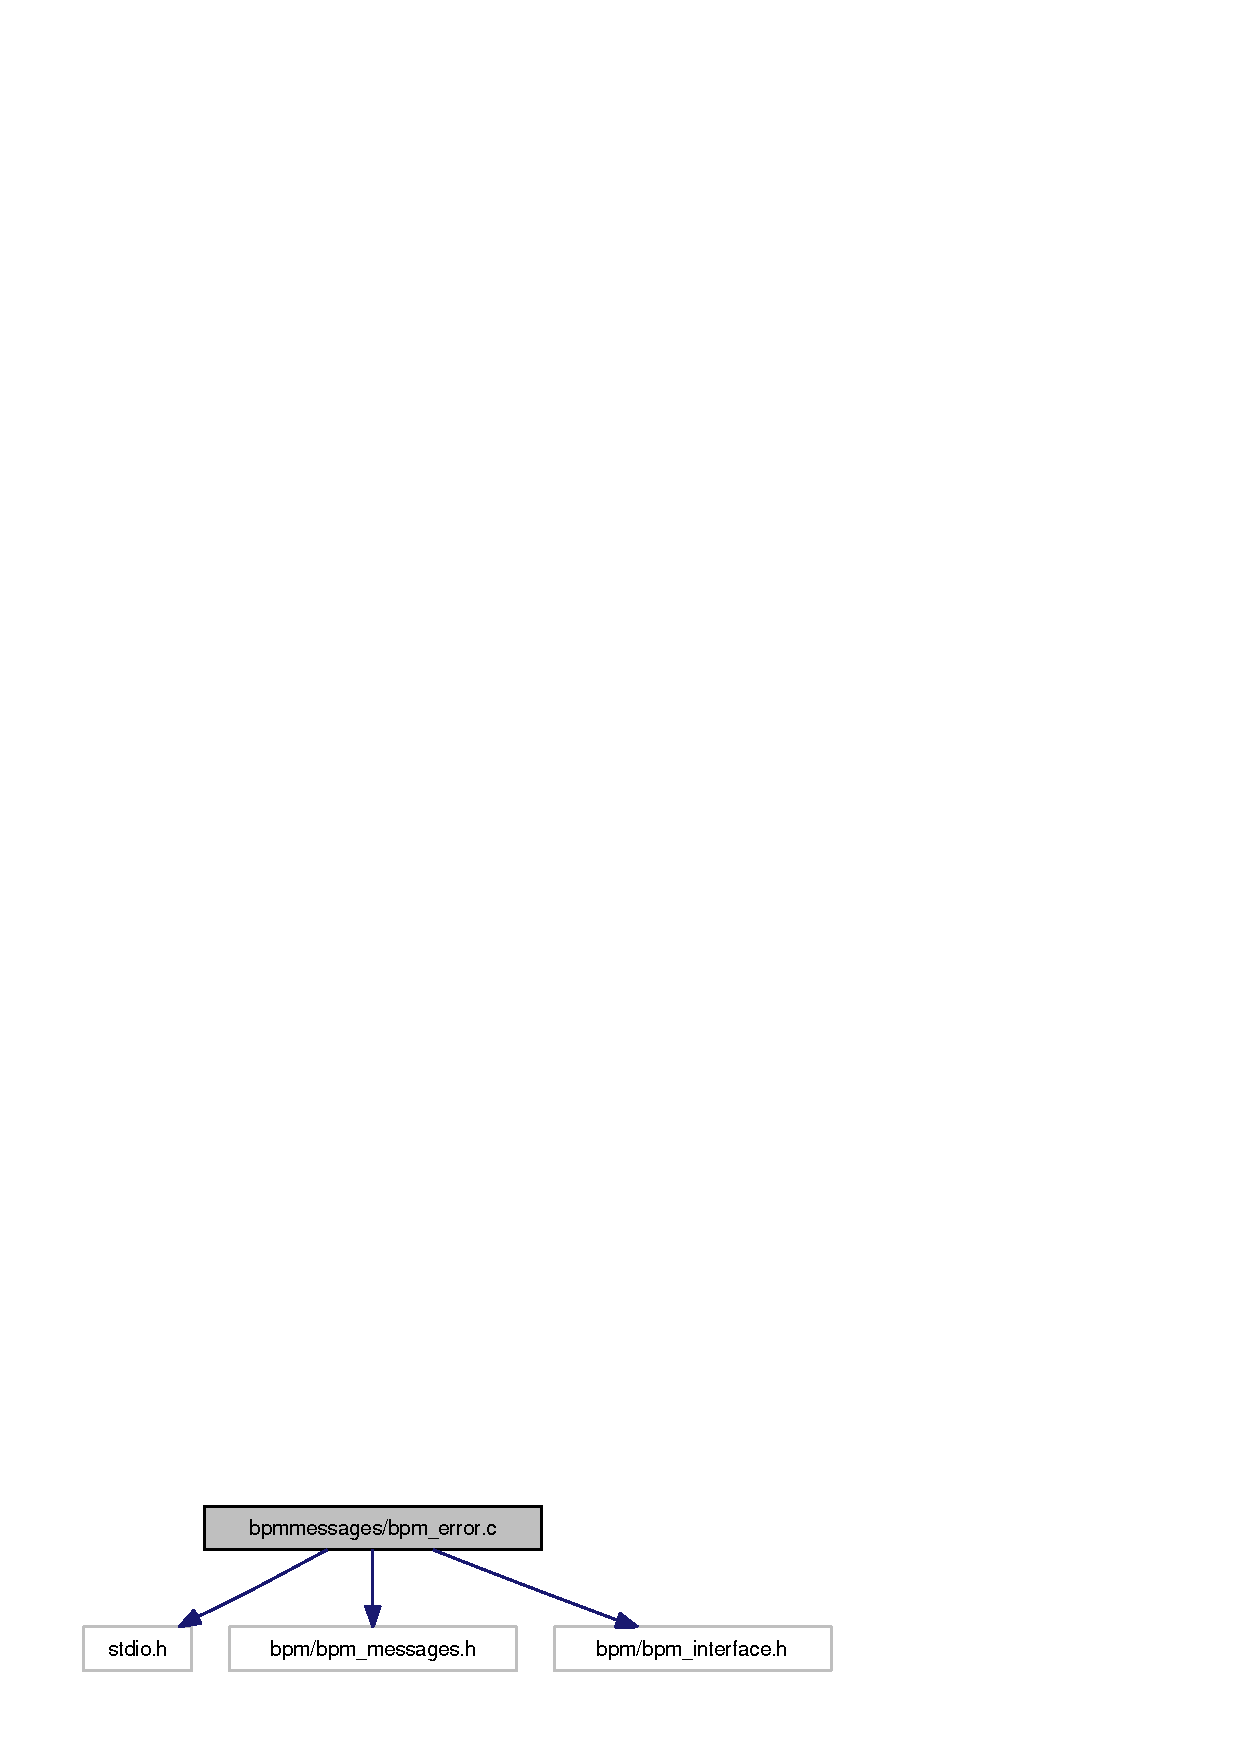
\includegraphics[width=201pt]{bpm__error_8c__incl}
\end{center}
\end{figure}
\subsubsection*{Functions}
\begin{CompactItemize}
\item 
void {\bf bpm\_\-error} (char $\ast$msg, char $\ast$f, int l)
\end{CompactItemize}

\subsection{bpmmessages/bpm\_\-messages.h File Reference}
\label{bpm__messages_8h}\index{bpmmessages/bpm\_\-messages.h@{bpmmessages/bpm\_\-messages.h}}


\subsubsection{Detailed Description}
libbpm error/warning messages 

This header defines the routines which take care of printing error and warning messages 

Definition in file {\bf bpm\_\-messages.h}.

{\tt \#include $<$bpm/bpm\_\-defs.h$>$}\par


Include dependency graph for bpm\_\-messages.h:\nopagebreak
\begin{figure}[H]
\begin{center}
\leavevmode
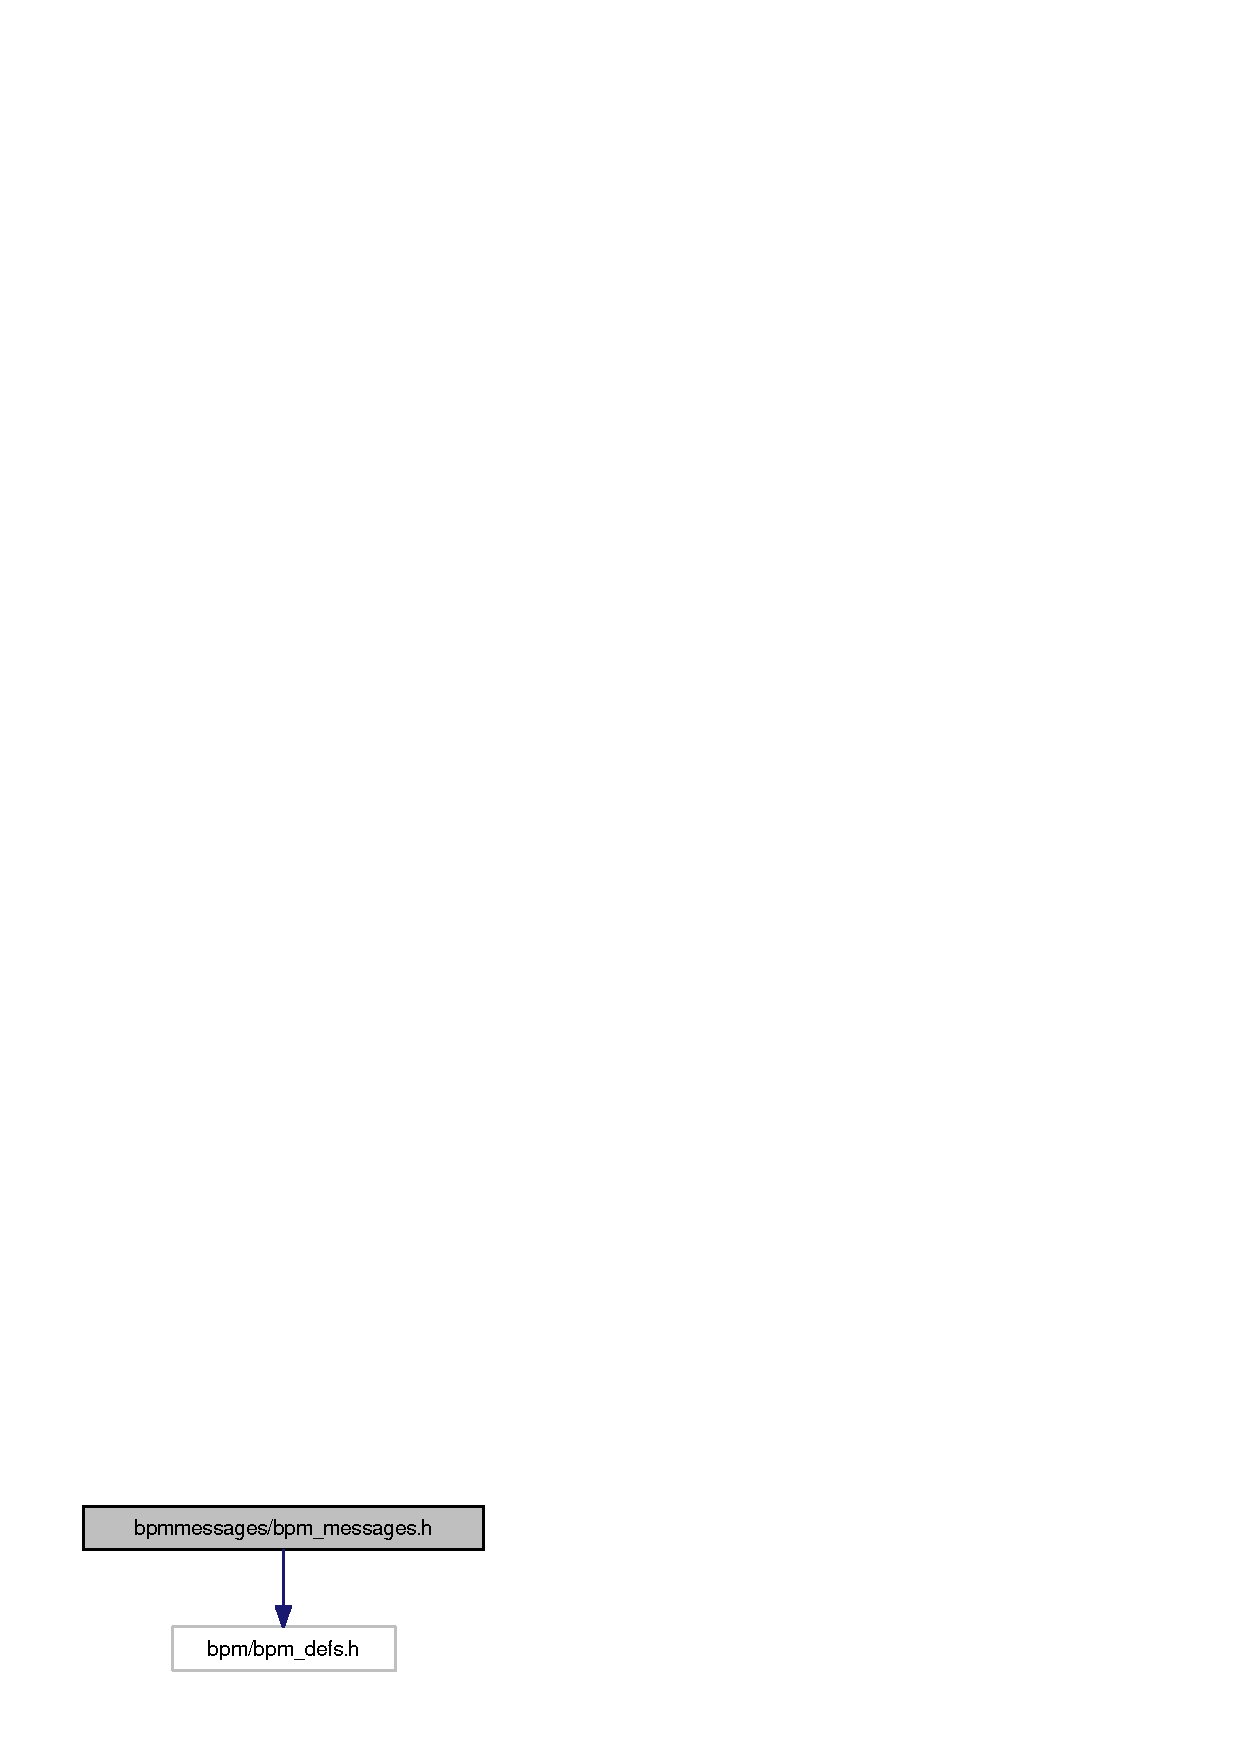
\includegraphics[width=118pt]{bpm__messages_8h__incl}
\end{center}
\end{figure}
\subsubsection*{Functions}
\begin{CompactItemize}
\item 
EXTERN void {\bf bpm\_\-error} (char $\ast$msg, char $\ast$f, int l)
\item 
EXTERN void {\bf bpm\_\-warning} (char $\ast$msg, char $\ast$f, int l)
\end{CompactItemize}

\subsection{bpmmessages/bpm\_\-warning.c File Reference}
\label{bpm__warning_8c}\index{bpmmessages/bpm\_\-warning.c@{bpmmessages/bpm\_\-warning.c}}


\subsubsection{Detailed Description}


Definition in file {\bf bpm\_\-warning.c}.

{\tt \#include $<$stdio.h$>$}\par
{\tt \#include $<$bpm/bpm\_\-messages.h$>$}\par
{\tt \#include $<$bpm/bpm\_\-interface.h$>$}\par


Include dependency graph for bpm\_\-warning.c:\nopagebreak
\begin{figure}[H]
\begin{center}
\leavevmode
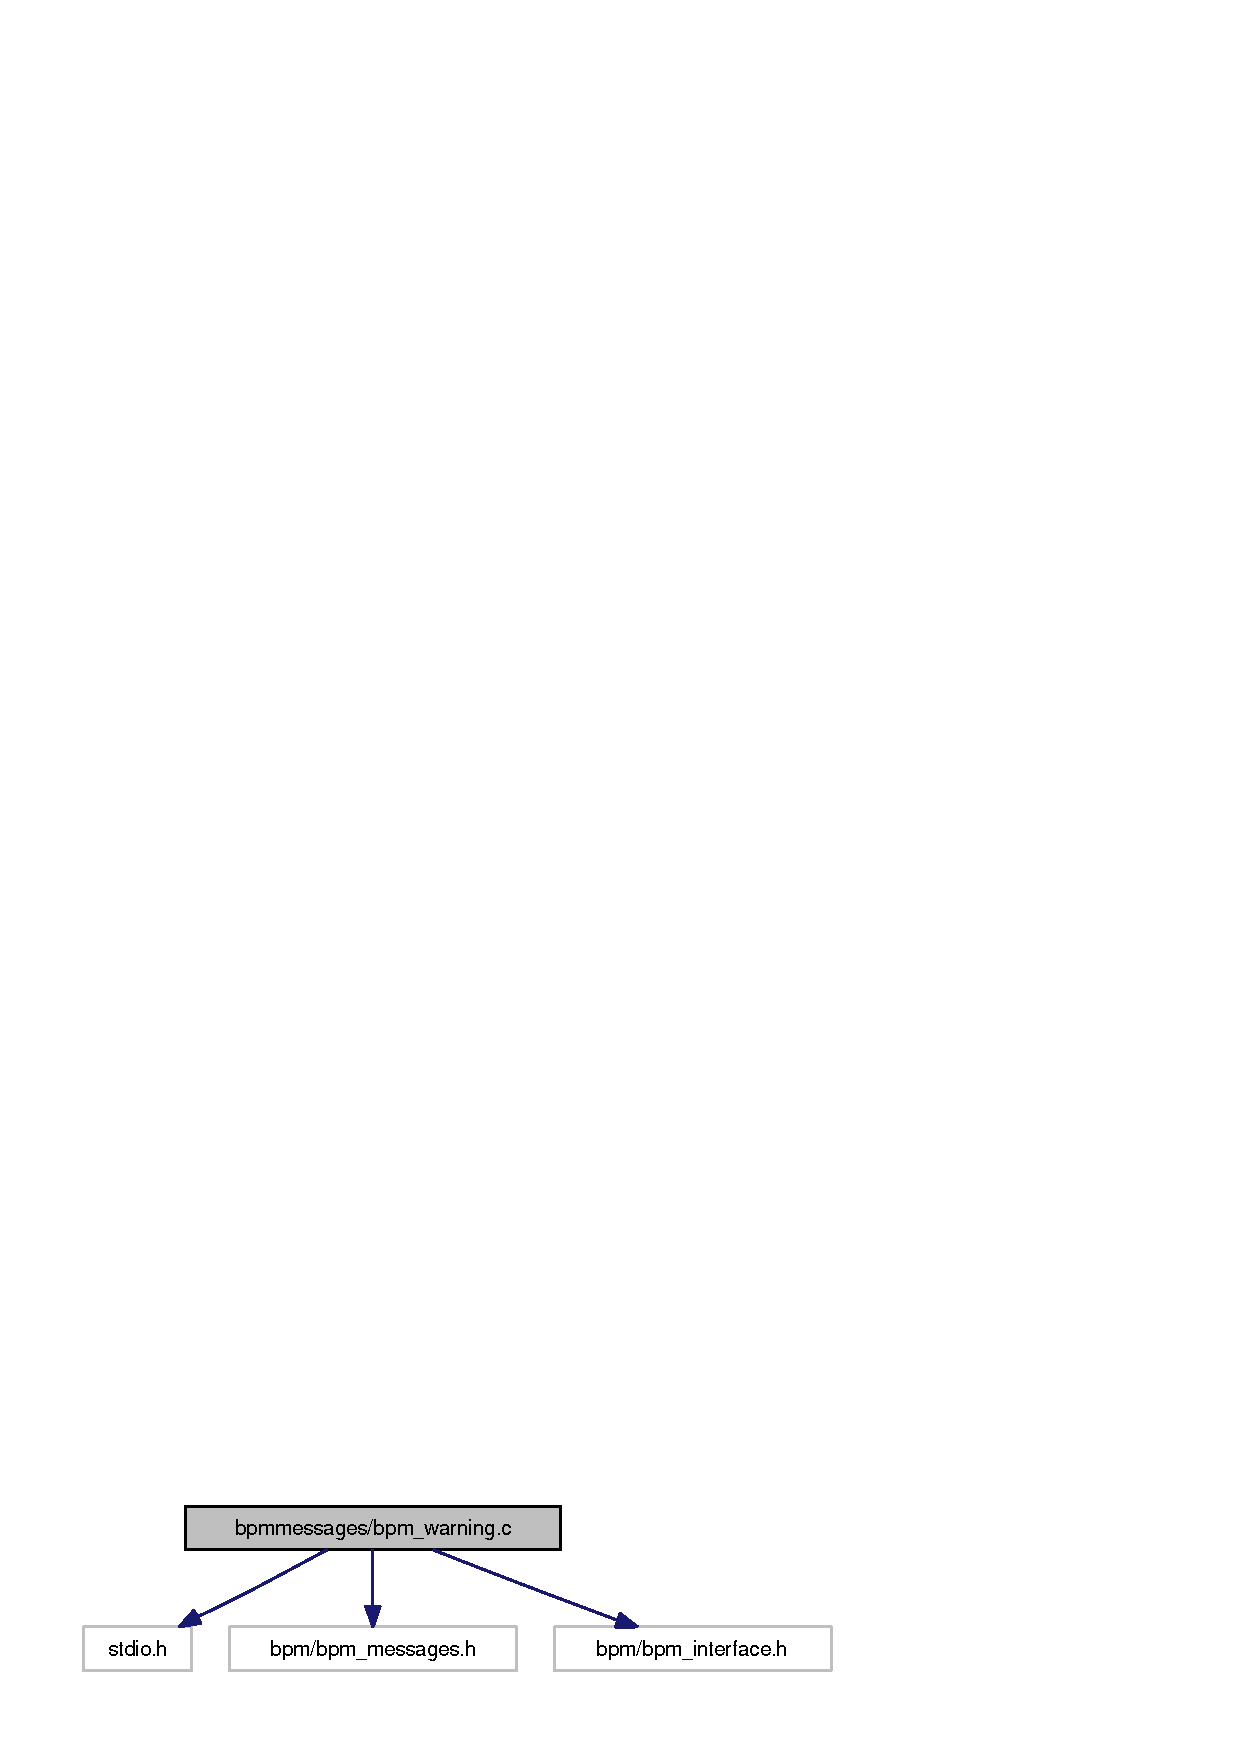
\includegraphics[width=201pt]{bpm__warning_8c__incl}
\end{center}
\end{figure}
\subsubsection*{Functions}
\begin{CompactItemize}
\item 
void {\bf bpm\_\-warning} (char $\ast$msg, char $\ast$f, int l)
\end{CompactItemize}

\subsection{bpmnr/bpm\_\-nr.h File Reference}
\label{bpm__nr_8h}\index{bpmnr/bpm\_\-nr.h@{bpmnr/bpm\_\-nr.h}}


\subsubsection{Detailed Description}
libbpm numerical helper routines 

Header file containing the numerical recipies and GNU Scientific Library routines used in the library. 

Definition in file {\bf bpm\_\-nr.h}.

{\tt \#include $<$stdio.h$>$}\par
{\tt \#include $<$stdlib.h$>$}\par
{\tt \#include $<$math.h$>$}\par
{\tt \#include $<$float.h$>$}\par
{\tt \#include $<$string.h$>$}\par
{\tt \#include $<$bpm/bpm\_\-defs.h$>$}\par


Include dependency graph for bpm\_\-nr.h:\nopagebreak
\begin{figure}[H]
\begin{center}
\leavevmode
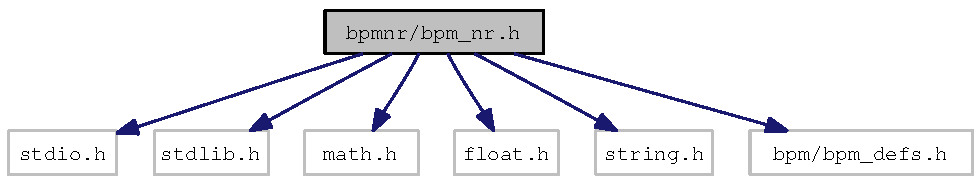
\includegraphics[width=253pt]{bpm__nr_8h__incl}
\end{center}
\end{figure}


This graph shows which files directly or indirectly include this file:\nopagebreak
\begin{figure}[H]
\begin{center}
\leavevmode
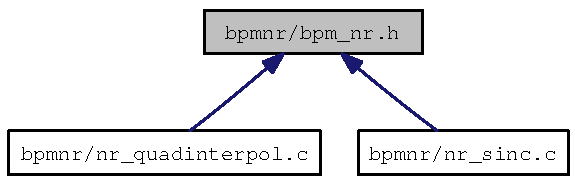
\includegraphics[width=156pt]{bpm__nr_8h__dep__incl}
\end{center}
\end{figure}
\subsubsection*{Data Structures}
\begin{CompactItemize}
\item 
struct {\bf lm\_\-fstate}
\item 
struct \textbf{gsl\_\-block\_\-struct}
\item 
struct \textbf{gsl\_\-matrix}
\item 
struct \textbf{\_\-gsl\_\-matrix\_\-view}
\item 
struct \textbf{gsl\_\-vector}
\item 
struct \textbf{\_\-gsl\_\-vector\_\-view}
\item 
struct \textbf{\_\-gsl\_\-vector\_\-const\_\-view}
\item 
struct {\bf complex\_\-t}
\end{CompactItemize}
\subsubsection*{Defines}
\begin{CompactItemize}
\item 
\#define {\bf GCF\_\-ITMAX}
\item 
\#define \textbf{GCF\_\-FPMIN}\label{group__nr_g4d2a5b0ed774d7c6cd7ed3aeede02b32}

\item 
\#define \textbf{GCF\_\-EPS}\label{group__nr_g545baaa7a8baff47a88f64d9e22f85eb}

\item 
\#define \textbf{GSER\_\-EPS}\label{group__nr_g2f99393cf98b977fa0ed7d77df4b1847}

\item 
\#define \textbf{GSER\_\-ITMAX}\label{group__nr_ge81a5f817c0ccb9e9b21d0a93a69f1fb}

\item 
\#define \textbf{RAN1\_\-IA}\label{group__nr_gfac3e13315af7108196380d1e4626fff}

\item 
\#define \textbf{RAN1\_\-IM}\label{group__nr_g1854f35d8460beeacca2f0538495054e}

\item 
\#define \textbf{RAN1\_\-AM}\label{group__nr_ga1f56cea0760315b3d77f8d43c214b9f}

\item 
\#define \textbf{RAN1\_\-IQ}\label{group__nr_g62b55be906a8312d99fa219df59d2603}

\item 
\#define \textbf{RAN1\_\-IR}\label{group__nr_gd9837af690685692ba3b79204aacda7d}

\item 
\#define \textbf{RAN1\_\-NTAB}\label{group__nr_g9ed2ef7c12b486ed6bcaa2f865799f39}

\item 
\#define \textbf{RAN1\_\-NDIV}\label{group__nr_g9e50163471f8a66724a30e90b859683c}

\item 
\#define \textbf{RAN1\_\-EPS}\label{group__nr_ge7332177f9233d665df2bc8b162d2484}

\item 
\#define \textbf{RAN1\_\-RNMX}\label{group__nr_g764a79bfff270bb14a93930e3da5d7cc}

\item 
\#define {\bf \_\-\_\-LM\_\-BLOCKSZ\_\-\_\-}
\item 
\#define \textbf{\_\-\_\-LM\_\-BLOCKSZ\_\-\_\-SQ}\label{group__nr_ge730cf8f762cf844c8a987af6be4bd9c}

\item 
\#define \textbf{LINSOLVERS\_\-RETAIN\_\-MEMORY}\label{group__nr_g24a049e550264f1529e47347e9753f7e}

\item 
\#define \textbf{\_\-\_\-LM\_\-STATIC\_\-\_\-}\label{group__nr_gf3381d1cf7cf6839730587497fb744b7}

\item 
\#define \textbf{FABS}(x)\label{group__nr_g9b649f4d878e64a80b4cd2cad45f43b3}

\item 
\#define \textbf{CNST}(x)\label{group__nr_g8097f2f4c007bf8d2ea1e7558b2248e0}

\item 
\#define \textbf{\_\-LM\_\-POW\_\-}\label{group__nr_gb28c2198a94b5c5508ab04b28e31aed2}

\item 
\#define {\bf LM\_\-DER\_\-WORKSZ}(npar, nmeas)
\item 
\#define {\bf LM\_\-DIF\_\-WORKSZ}(npar, nmeas)
\item 
\#define \textbf{LM\_\-EPSILON}\label{group__nr_g4bd7ce4e1f4cc6be913fc6a383bce112}

\item 
\#define \textbf{LM\_\-ONE\_\-THIRD}\label{group__nr_g307e270c028a33b97c90f66245f81452}

\item 
\#define \textbf{LM\_\-OPTS\_\-SZ}\label{group__nr_ge3ee35a37fd4d8532ac769d5bd372a53}

\item 
\#define \textbf{LM\_\-INFO\_\-SZ}\label{group__nr_g20fee96f47f09233385fb107510b45da}

\item 
\#define \textbf{LM\_\-INIT\_\-MU}\label{group__nr_g6664bcbe28414c3df4b36063a6823d0c}

\item 
\#define \textbf{LM\_\-STOP\_\-THRESH}\label{group__nr_g344f3598e6156022e8c5175b060d9201}

\item 
\#define \textbf{LM\_\-DIFF\_\-DELTA}\label{group__nr_g0560e7d9a262a0c72f156639096a261d}

\item 
\#define {\bf NR\_\-FFTFORWARD}
\item 
\#define {\bf NR\_\-FFTBACKWARD}
\item 
\#define {\bf \_\-\_\-LM\_\-MEDIAN3}(a, b, c)
\item 
\#define \textbf{NULL\_\-VECTOR}\label{group__nr_g9839236a6f8b2f71c017c7ad3564c12d}

\item 
\#define \textbf{NULL\_\-VECTOR\_\-VIEW}\label{group__nr_gd53a17dfdfc936b7559bdc08efbe1c7e}

\item 
\#define \textbf{NULL\_\-MATRIX}\label{group__nr_g9aaa363ea623569297d0fced07b4b263}

\item 
\#define \textbf{NULL\_\-MATRIX\_\-VIEW}\label{group__nr_g2c402132fe8822a31f21b968666fa188}

\item 
\#define \textbf{GSL\_\-DBL\_\-EPSILON}\label{group__nr_g2ee9a14250ef1c11d3a454c93703de4e}

\item 
\#define \textbf{OFFSET}(N, incX)\label{group__nr_g098f1989e95be172fad854c44d1be6ee}

\item 
\#define \textbf{GSL\_\-MIN}(a, b)\label{group__nr_ga97847b845ae5d3fbbec4d2d8ec3310d}

\end{CompactItemize}
\subsubsection*{Typedefs}
\begin{CompactItemize}
\item 
typedef enum CBLAS\_\-TRANSPOSE \textbf{CBLAS\_\-TRANSPOSE\_\-t}\label{group__nr_gfe7082539a5d26f5c498526d07ebe8d3}

\item 
typedef struct gsl\_\-block\_\-struct \textbf{gsl\_\-block}\label{group__nr_g3858db8a10651ceb818008b6db3fed1e}

\item 
typedef \_\-gsl\_\-matrix\_\-view \textbf{gsl\_\-matrix\_\-view}\label{group__nr_g8aacfa9dbffc4c6918036c329437dc40}

\item 
typedef \_\-gsl\_\-vector\_\-view \textbf{gsl\_\-vector\_\-view}\label{group__nr_g2a9448788d5ea6053036f94bce37ca9b}

\item 
typedef const \_\-gsl\_\-vector\_\-const\_\-view \textbf{gsl\_\-vector\_\-const\_\-view}\label{group__nr_gcba10bedbc0a23130b5d8e52b83b925e}

\end{CompactItemize}
\subsubsection*{Enumerations}
\begin{CompactItemize}
\item 
enum \textbf{CBLAS\_\-TRANSPOSE} \{ \textbf{CblasNoTrans}, 
\textbf{CblasTrans}, 
\textbf{CblasConjTrans}
 \}
\item 
enum \textbf{CBLAS\_\-ORDER} \{ \textbf{CblasRowMajor}, 
\textbf{CblasColMajor}
 \}
\end{CompactItemize}
\subsubsection*{Functions}
\begin{CompactItemize}
\item 
EXTERN double {\bf nr\_\-gammln} (double xx)
\item 
EXTERN double {\bf nr\_\-gammq} (double a, double x)
\item 
EXTERN int {\bf nr\_\-gcf} (double $\ast$gammcf, double a, double x, double $\ast$gln)
\item 
EXTERN int {\bf nr\_\-gser} (double $\ast$gamser, double a, double x, double $\ast$gln)
\item 
EXTERN int {\bf nr\_\-fit} (double $\ast$x, double y[$\,$], int ndata, double sig[$\,$], int mwt, double $\ast$a, double $\ast$b, double $\ast$siga, double $\ast$sigb, double $\ast$chi2, double $\ast$q)
\item 
EXTERN int {\bf nr\_\-is\_\-pow2} (unsigned long n)
\item 
EXTERN int {\bf nr\_\-four1} (double data[$\,$], unsigned long nn, int isign)
\item 
EXTERN int {\bf nr\_\-realft} (double data[$\,$], unsigned long n, int isign)
\item 
EXTERN double {\bf nr\_\-ran1} (long $\ast$idum)
\item 
EXTERN int {\bf nr\_\-seed} (long seed)
\item 
EXTERN double {\bf nr\_\-ranuniform} (double lower, double upper)
\item 
EXTERN double {\bf nr\_\-rangauss} (double mean, double std\_\-dev)
\item 
EXTERN int \textbf{nr\_\-lmder} (void($\ast$func)(double $\ast$p, double $\ast$hx, int m, int n, void $\ast$adata), void($\ast$jacf)(double $\ast$p, double $\ast$j, int m, int n, void $\ast$adata), double $\ast$p, double $\ast$x, int m, int n, int itmax, double $\ast$opts, double $\ast$info, double $\ast$work, double $\ast$covar, void $\ast$adata)\label{group__nr_g59c2090d19b1ad8ed35f50e49539aa0a}

\item 
EXTERN int \textbf{nr\_\-lmdif} (void($\ast$func)(double $\ast$p, double $\ast$hx, int m, int n, void $\ast$adata), double $\ast$p, double $\ast$x, int m, int n, int itmax, double $\ast$opts, double $\ast$info, double $\ast$work, double $\ast$covar, void $\ast$adata)\label{group__nr_g352d4d338f80dc0fe3db4bac7dc9640e}

\item 
EXTERN int \textbf{nr\_\-lmder\_\-bc} (void($\ast$func)(double $\ast$p, double $\ast$hx, int m, int n, void $\ast$adata), void($\ast$jacf)(double $\ast$p, double $\ast$j, int m, int n, void $\ast$adata), double $\ast$p, double $\ast$x, int m, int n, double $\ast$lb, double $\ast$ub, int itmax, double $\ast$opts, double $\ast$info, double $\ast$work, double $\ast$covar, void $\ast$adata)\label{group__nr_g55db15253f85ccac7c985280705da745}

\item 
EXTERN int \textbf{nr\_\-lmdif\_\-bc} (void($\ast$func)(double $\ast$p, double $\ast$hx, int m, int n, void $\ast$adata), double $\ast$p, double $\ast$x, int m, int n, double $\ast$lb, double $\ast$ub, int itmax, double $\ast$opts, double $\ast$info, double $\ast$work, double $\ast$covar, void $\ast$adata)\label{group__nr_ga343a39b99f7bb25b97134a743a81a20}

\item 
EXTERN void \textbf{nr\_\-lmchkjac} (void($\ast$func)(double $\ast$p, double $\ast$hx, int m, int n, void $\ast$adata), void($\ast$jacf)(double $\ast$p, double $\ast$j, int m, int n, void $\ast$adata), double $\ast$p, int m, int n, void $\ast$adata, double $\ast$err)\label{group__nr_gc0c5d8dc11fc35234e751fbc54a6a185}

\item 
EXTERN int \textbf{nr\_\-lmcovar} (double $\ast$JtJ, double $\ast$C, double sumsq, int m, int n)\label{group__nr_g2e38d1d3a33b269e190fb0edd3fc3303}

\item 
EXTERN int \textbf{nr\_\-ax\_\-eq\_\-b\_\-LU} (double $\ast$A, double $\ast$B, double $\ast$x, int n)\label{group__nr_g50388d5d50f760129a054ea526ed1c07}

\item 
EXTERN void \textbf{nr\_\-trans\_\-mat\_\-mat\_\-mult} (double $\ast$a, double $\ast$b, int n, int m)\label{group__nr_gb647cf24b2b6ab2a0dd993ba4021447c}

\item 
EXTERN void \textbf{nr\_\-fdif\_\-forw\_\-jac\_\-approx} (void($\ast$func)(double $\ast$p, double $\ast$hx, int m, int n, void $\ast$adata), double $\ast$p, double $\ast$hx, double $\ast$hxx, double delta, double $\ast$jac, int m, int n, void $\ast$adata)\label{group__nr_gf20223185cc5c2a215cb6559231dd55b}

\item 
EXTERN void \textbf{nr\_\-fdif\_\-cent\_\-jac\_\-approx} (void($\ast$func)(double $\ast$p, double $\ast$hx, int m, int n, void $\ast$adata), double $\ast$p, double $\ast$hxm, double $\ast$hxp, double delta, double $\ast$jac, int m, int n, void $\ast$adata)\label{group__nr_geab4b93cc9d2f74f4c1859204fc9e694}

\item 
EXTERN double {\bf nr\_\-median} (int n, double $\ast$arr)
\item 
EXTERN double {\bf nr\_\-select} (int k, int n, double $\ast$org\_\-arr)
\item 
EXTERN gsl\_\-matrix $\ast$ \textbf{gsl\_\-matrix\_\-calloc} (const size\_\-t n1, const size\_\-t n2)\label{group__nr_gf2e18583a2759c9d0f78b564f40eccd7}

\item 
EXTERN \_\-gsl\_\-vector\_\-view {\bf gsl\_\-matrix\_\-column} (gsl\_\-matrix $\ast$m, const size\_\-t i)
\item 
EXTERN \_\-gsl\_\-matrix\_\-view {\bf gsl\_\-matrix\_\-submatrix} (gsl\_\-matrix $\ast$m, const size\_\-t i, const size\_\-t j, const size\_\-t n1, const size\_\-t n2)
\item 
EXTERN double {\bf gsl\_\-matrix\_\-get} (const gsl\_\-matrix $\ast$m, const size\_\-t i, const size\_\-t j)
\item 
EXTERN void {\bf gsl\_\-matrix\_\-set} (gsl\_\-matrix $\ast$m, const size\_\-t i, const size\_\-t j, const double x)
\item 
EXTERN int {\bf gsl\_\-matrix\_\-swap\_\-columns} (gsl\_\-matrix $\ast$m, const size\_\-t i, const size\_\-t j)
\item 
EXTERN gsl\_\-matrix $\ast$ \textbf{gsl\_\-matrix\_\-alloc} (const size\_\-t n1, const size\_\-t n2)\label{group__nr_g3c416b23f730c2e06cb5e9b257f1f571}

\item 
EXTERN \_\-gsl\_\-vector\_\-const\_\-view \textbf{gsl\_\-matrix\_\-const\_\-row} (const gsl\_\-matrix $\ast$m, const size\_\-t i)\label{group__nr_g1b0f557b9e570f397ab13dcc24e09e35}

\item 
EXTERN \_\-gsl\_\-vector\_\-view \textbf{gsl\_\-matrix\_\-row} (gsl\_\-matrix $\ast$m, const size\_\-t i)\label{group__nr_gebf16339184d6759f4cdfa9c1724fb98}

\item 
EXTERN \_\-gsl\_\-vector\_\-const\_\-view \textbf{gsl\_\-matrix\_\-const\_\-column} (const gsl\_\-matrix $\ast$m, const size\_\-t j)\label{group__nr_gf288953bef254a8e2221d778c28f7f97}

\item 
EXTERN void \textbf{gsl\_\-matrix\_\-set\_\-identity} (gsl\_\-matrix $\ast$m)\label{group__nr_ge37f3f441742e70b1a701d92446e33fc}

\item 
EXTERN gsl\_\-vector $\ast$ \textbf{gsl\_\-vector\_\-calloc} (const size\_\-t n)\label{group__nr_gac4c2937f0e28c7a00cfe90b4ad886a6}

\item 
EXTERN \_\-gsl\_\-vector\_\-view {\bf gsl\_\-vector\_\-subvector} (gsl\_\-vector $\ast$v, size\_\-t offset, size\_\-t n)
\item 
EXTERN double {\bf gsl\_\-vector\_\-get} (const gsl\_\-vector $\ast$v, const size\_\-t i)
\item 
EXTERN void {\bf gsl\_\-vector\_\-set} (gsl\_\-vector $\ast$v, const size\_\-t i, double x)
\item 
EXTERN int \textbf{gsl\_\-vector\_\-swap\_\-elements} (gsl\_\-vector $\ast$v, const size\_\-t i, const size\_\-t j)\label{group__nr_g2624694e4157398ba344b90eca6ba070}

\item 
EXTERN \_\-gsl\_\-vector\_\-const\_\-view \textbf{gsl\_\-vector\_\-const\_\-subvector} (const gsl\_\-vector $\ast$v, size\_\-t i, size\_\-t n)\label{group__nr_ga45e4b3770af5d15171055314b140838}

\item 
EXTERN void \textbf{gsl\_\-vector\_\-free} (gsl\_\-vector $\ast$v)\label{group__nr_gedc84887915223f87986de6a67c0249d}

\item 
EXTERN int \textbf{gsl\_\-linalg\_\-SV\_\-solve} (const gsl\_\-matrix $\ast$U, const gsl\_\-matrix $\ast$Q, const gsl\_\-vector $\ast$S, const gsl\_\-vector $\ast$b, gsl\_\-vector $\ast$x)\label{group__nr_g8568eb30743233bab6e1c2d530829f5f}

\item 
EXTERN int \textbf{gsl\_\-linalg\_\-bidiag\_\-unpack} (const gsl\_\-matrix $\ast$A, const gsl\_\-vector $\ast$tau\_\-U, gsl\_\-matrix $\ast$U, const gsl\_\-vector $\ast$tau\_\-V, gsl\_\-matrix $\ast$V, gsl\_\-vector $\ast$diag, gsl\_\-vector $\ast$superdiag)\label{group__nr_gc4843a336042d90bbacea983a80e29b9}

\item 
EXTERN int {\bf gsl\_\-linalg\_\-householder\_\-hm} (double tau, const gsl\_\-vector $\ast$v, gsl\_\-matrix $\ast$A)
\item 
EXTERN int \textbf{gsl\_\-linalg\_\-bidiag\_\-unpack2} (gsl\_\-matrix $\ast$A, gsl\_\-vector $\ast$tau\_\-U, gsl\_\-vector $\ast$tau\_\-V, gsl\_\-matrix $\ast$V)\label{group__nr_g4881575010a0877aba5efab6f368ab8c}

\item 
EXTERN int {\bf gsl\_\-linalg\_\-householder\_\-hm1} (double tau, gsl\_\-matrix $\ast$A)
\item 
EXTERN void \textbf{create\_\-givens} (const double a, const double b, double $\ast$c, double $\ast$s)\label{group__nr_g2c1eb13f0c90da0f8ef4ef712db29f44}

\item 
EXTERN double {\bf gsl\_\-linalg\_\-householder\_\-transform} (gsl\_\-vector $\ast$v)
\item 
EXTERN int {\bf gsl\_\-linalg\_\-householder\_\-mh} (double tau, const gsl\_\-vector $\ast$v, gsl\_\-matrix $\ast$A)
\item 
EXTERN void \textbf{chop\_\-small\_\-elements} (gsl\_\-vector $\ast$d, gsl\_\-vector $\ast$f)\label{group__nr_g7a9b4689f2fcd8d6a417a071903df6f1}

\item 
EXTERN void \textbf{qrstep} (gsl\_\-vector $\ast$d, gsl\_\-vector $\ast$f, gsl\_\-matrix $\ast$U, gsl\_\-matrix $\ast$V)\label{group__nr_g8e5d28fda0cf04d6d70392fa9580c2eb}

\item 
EXTERN double \textbf{trailing\_\-eigenvalue} (const gsl\_\-vector $\ast$d, const gsl\_\-vector $\ast$f)\label{group__nr_g615603d99ef3bb2a21b32e13761a1474}

\item 
EXTERN void \textbf{create\_\-schur} (double d0, double f0, double d1, double $\ast$c, double $\ast$s)\label{group__nr_g31a6def59f109d51a7e9af63a8850f0c}

\item 
EXTERN void \textbf{svd2} (gsl\_\-vector $\ast$d, gsl\_\-vector $\ast$f, gsl\_\-matrix $\ast$U, gsl\_\-matrix $\ast$V)\label{group__nr_ge8a1bf5b51ec0f7ef1e067f01d466033}

\item 
EXTERN void \textbf{chase\_\-out\_\-intermediate\_\-zero} (gsl\_\-vector $\ast$d, gsl\_\-vector $\ast$f, gsl\_\-matrix $\ast$U, size\_\-t k0)\label{group__nr_g1b67ba06b6b7daa4f73a163f404dd3d7}

\item 
EXTERN void \textbf{chase\_\-out\_\-trailing\_\-zero} (gsl\_\-vector $\ast$d, gsl\_\-vector $\ast$f, gsl\_\-matrix $\ast$V)\label{group__nr_g15f37e448cf7eabd56ec2c351f148214}

\item 
EXTERN int \textbf{gsl\_\-isnan} (const double x)\label{group__nr_gf37b7182e24399515692cc4aa39722dd}

\item 
EXTERN double {\bf gsl\_\-blas\_\-dnrm2} (const gsl\_\-vector $\ast$X)
\item 
EXTERN double \textbf{cblas\_\-dnrm2} (const int N, const double $\ast$X, const int incX)\label{group__nr_g7201c3bc9f98c0b703b326b9178c4965}

\item 
EXTERN void \textbf{gsl\_\-blas\_\-dscal} (double alpha, gsl\_\-vector $\ast$X)\label{group__nr_g549aa3e6fac9f177535de54692d31df8}

\item 
EXTERN void \textbf{cblas\_\-dscal} (const int N, const double alpha, double $\ast$X, const int incX)\label{group__nr_ge13bffd83c5432842602645c03f6f26a}

\item 
EXTERN void \textbf{cblas\_\-dgemv} (const enum CBLAS\_\-ORDER order, const enum CBLAS\_\-TRANSPOSE TransA, const int M, const int N, const double alpha, const double $\ast$A, const int lda, const double $\ast$X, const int incX, const double beta, double $\ast$Y, const int incY)\label{group__nr_g71539c2ec3663bb7ec3bc88882da603a}

\item 
EXTERN gsl\_\-block $\ast$ {\bf gsl\_\-block\_\-alloc} (const size\_\-t n)
\item 
EXTERN void \textbf{gsl\_\-block\_\-free} (gsl\_\-block $\ast$b)\label{group__nr_g0952127372c14dce3c3aa65ec0ad9c1e}

\item 
EXTERN {\bf complex\_\-t} \textbf{complex} (double re, double im)\label{group__nr_g203888bac468229094352b2bb9456417}

\item 
EXTERN double \textbf{c\_\-real} ({\bf complex\_\-t} z)\label{group__nr_gbd9dcd9992cad1f6af326811da66fc9a}

\item 
EXTERN double \textbf{c\_\-imag} ({\bf complex\_\-t} z)\label{group__nr_g6adc8ee3a56fe88de97c3f40c484f824}

\item 
EXTERN {\bf complex\_\-t} \textbf{c\_\-conj} ({\bf complex\_\-t} z)\label{group__nr_g26f4378875ac801b1b5bb7a13f180f0a}

\item 
EXTERN {\bf complex\_\-t} \textbf{c\_\-neg} ({\bf complex\_\-t} z)\label{group__nr_g33f198bcc4dd193c4f8c8db9049311d2}

\item 
EXTERN {\bf complex\_\-t} \textbf{c\_\-sum} ({\bf complex\_\-t} z1, {\bf complex\_\-t} z2)\label{group__nr_g176d351f4b035de54e1fb9974c296bed}

\item 
EXTERN {\bf complex\_\-t} \textbf{c\_\-diff} ({\bf complex\_\-t} z1, {\bf complex\_\-t} z2)\label{group__nr_g5b48402b525952efb744f5b2804d1957}

\item 
EXTERN {\bf complex\_\-t} \textbf{c\_\-mult} ({\bf complex\_\-t} z1, {\bf complex\_\-t} z2)\label{group__nr_gbac492f503bff737e6a11c03e44e7ada}

\item 
EXTERN {\bf complex\_\-t} \textbf{c\_\-div} ({\bf complex\_\-t} z1, {\bf complex\_\-t} z2)\label{group__nr_g3cb3d7ddec167a30a5f7a159dea26c0f}

\item 
EXTERN {\bf complex\_\-t} \textbf{c\_\-scale} (double r, {\bf complex\_\-t} z)\label{group__nr_g4a8c814a8cb7b92c919b23e1ea64d615}

\item 
EXTERN {\bf complex\_\-t} \textbf{c\_\-sqr} ({\bf complex\_\-t} z)\label{group__nr_g72516630e1d745f5d1630b4c525cb5f8}

\item 
EXTERN {\bf complex\_\-t} \textbf{c\_\-sqrt} ({\bf complex\_\-t} z)\label{group__nr_g22d2bd8775120d34e3b700682e67d955}

\item 
EXTERN double \textbf{c\_\-norm2} ({\bf complex\_\-t} z)\label{group__nr_g98f394b1ddccfeb4d9b5edb6c1f8c652}

\item 
EXTERN double \textbf{c\_\-abs} ({\bf complex\_\-t} z)\label{group__nr_gdd54790aa13824ee1db3d0558a465071}

\item 
EXTERN double \textbf{c\_\-abs2} ({\bf complex\_\-t} z)\label{group__nr_g5a31b290dd721358e4270d9686347dde}

\item 
EXTERN double \textbf{c\_\-arg} ({\bf complex\_\-t} z)\label{group__nr_g5a8776cef7d6ef88a11015d6ec2665ba}

\item 
EXTERN {\bf complex\_\-t} \textbf{c\_\-exp} ({\bf complex\_\-t} z)\label{group__nr_g41a40da9e1d42de8e76d999abd476f8a}

\item 
EXTERN int \textbf{c\_\-isequal} ({\bf complex\_\-t} z1, {\bf complex\_\-t} z2)\label{group__nr_gd3e4d63450915ff27b8e506acb21bb2e}

\item 
EXTERN double {\bf nr\_\-quadinterpol} (double x, double x1, double x2, double x3, double y1, double y2, double y3)
\item 
EXTERN double {\bf sinc} (double x)
\item 
EXTERN double {\bf lanczos} (double x, int a)
\item 
EXTERN double {\bf dround} (double x)
\end{CompactItemize}
\subsubsection*{Variables}
\begin{CompactItemize}
\item 
EXTERN long \textbf{bpm\_\-rseed}\label{group__nr_ga0d31375f4ee67d90ba46fbda872d25c}

\end{CompactItemize}

\subsection{bpmnr/dround.c File Reference}
\label{dround_8c}\index{bpmnr/dround.c@{bpmnr/dround.c}}


\subsubsection{Detailed Description}


Definition in file {\bf dround.c}.

\subsubsection*{Functions}
\begin{CompactItemize}
\item 
double {\bf dround} (double x)
\end{CompactItemize}

\subsection{bpmnr/gsl\_\-blas.c File Reference}
\label{gsl__blas_8c}\index{bpmnr/gsl\_\-blas.c@{bpmnr/gsl\_\-blas.c}}


\subsubsection{Detailed Description}


Definition in file {\bf gsl\_\-blas.c}.

{\tt \#include $<$bpm/bpm\_\-messages.h$>$}\par
{\tt \#include $<$bpm/bpm\_\-nr.h$>$}\par


Include dependency graph for gsl\_\-blas.c:\nopagebreak
\begin{figure}[H]
\begin{center}
\leavevmode
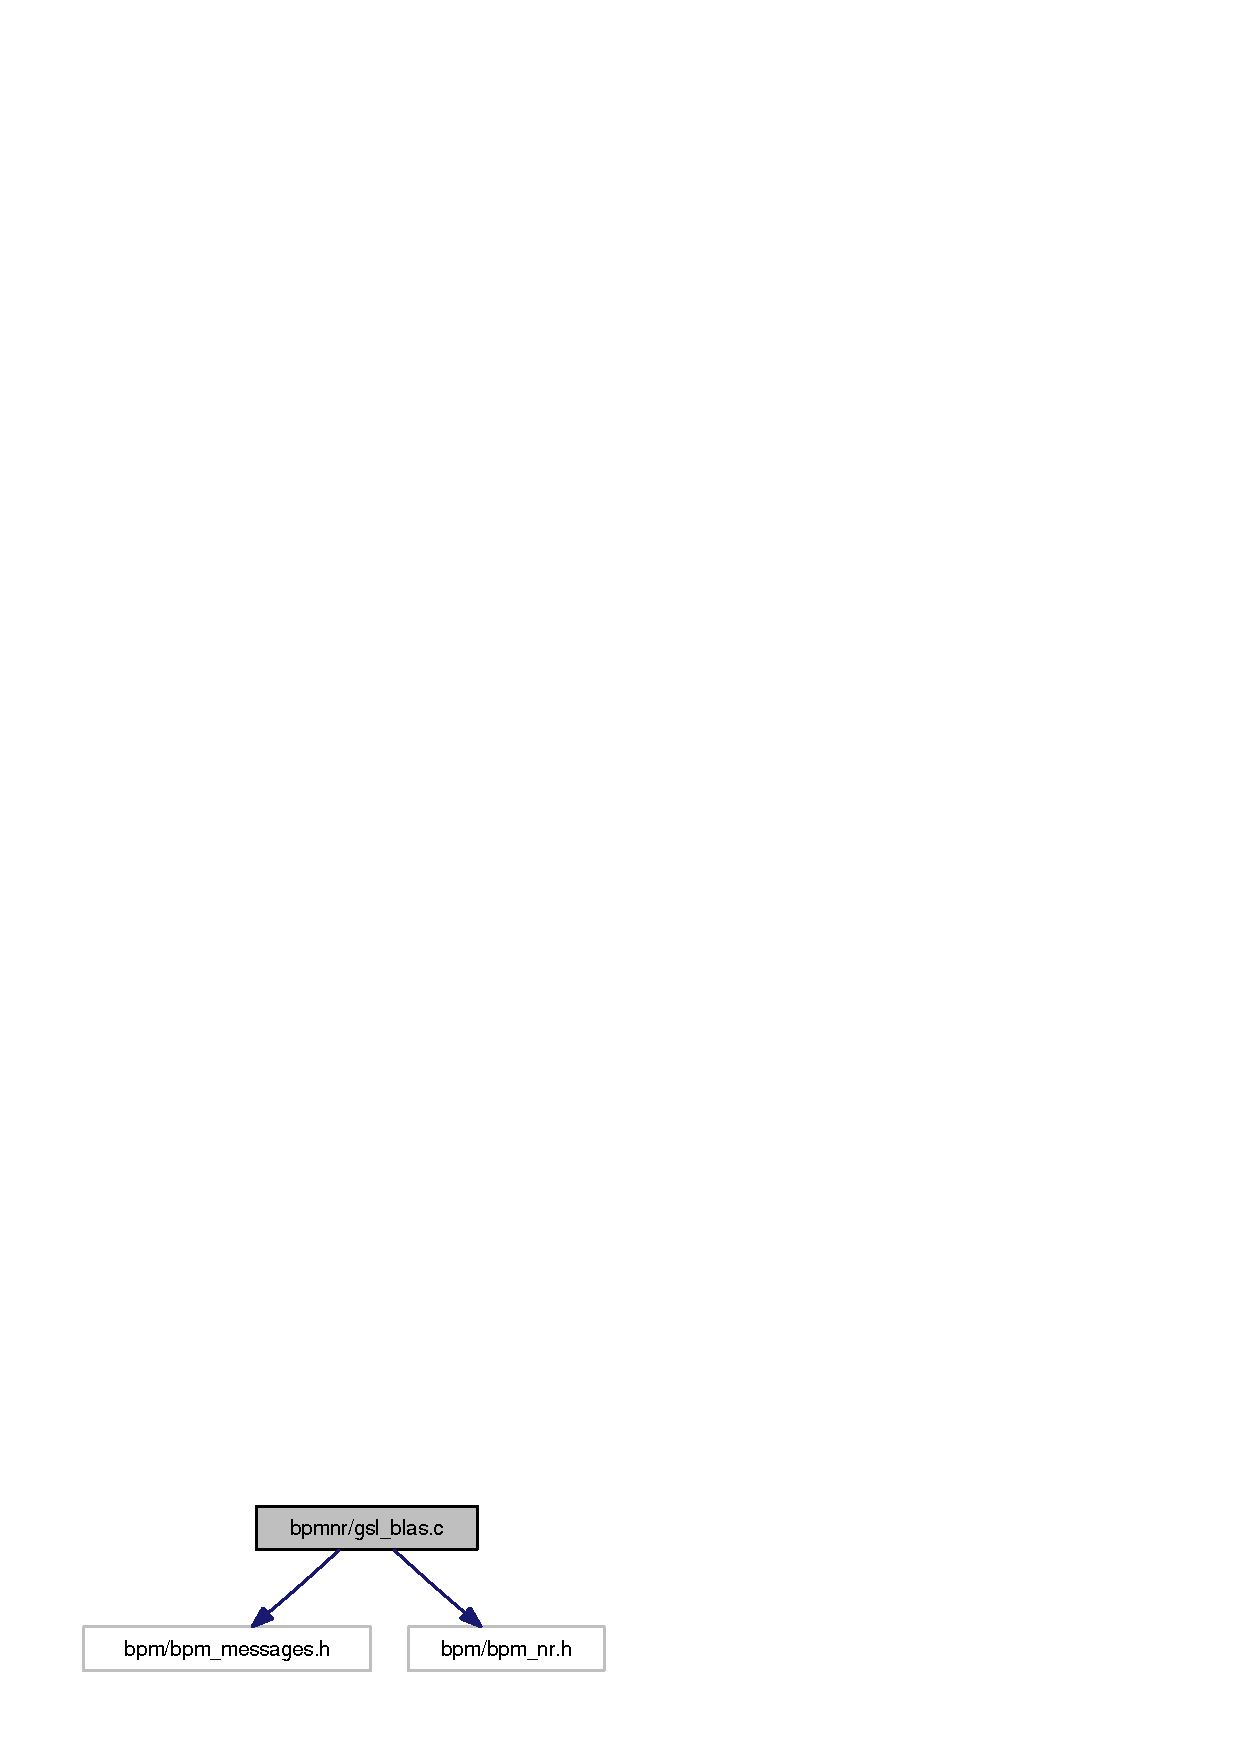
\includegraphics[width=147pt]{gsl__blas_8c__incl}
\end{center}
\end{figure}
\subsubsection*{Functions}
\begin{CompactItemize}
\item 
double {\bf gsl\_\-blas\_\-dnrm2} (const gsl\_\-vector $\ast$X)
\item 
double \textbf{cblas\_\-dnrm2} (const int N, const double $\ast$X, const int incX)\label{group__nr_g7201c3bc9f98c0b703b326b9178c4965}

\item 
void \textbf{gsl\_\-blas\_\-dscal} (double alpha, gsl\_\-vector $\ast$X)\label{group__nr_g549aa3e6fac9f177535de54692d31df8}

\item 
void \textbf{cblas\_\-dscal} (const int N, const double alpha, double $\ast$X, const int incX)\label{group__nr_ge13bffd83c5432842602645c03f6f26a}

\item 
int \textbf{gsl\_\-blas\_\-dgemv} (CBLAS\_\-TRANSPOSE\_\-t TransA, double alpha, const gsl\_\-matrix $\ast$A, const gsl\_\-vector $\ast$X, double beta, gsl\_\-vector $\ast$Y)\label{gsl__blas_8c_e75ae29cba0f1bf3c9293e4a993d4cd9}

\item 
void \textbf{cblas\_\-dgemv} (const enum CBLAS\_\-ORDER order, const enum CBLAS\_\-TRANSPOSE TransA, const int M, const int N, const double alpha, const double $\ast$A, const int lda, const double $\ast$X, const int incX, const double beta, double $\ast$Y, const int incY)\label{group__nr_g71539c2ec3663bb7ec3bc88882da603a}

\end{CompactItemize}

\subsection{bpmnr/gsl\_\-block.c File Reference}
\label{gsl__block_8c}\index{bpmnr/gsl\_\-block.c@{bpmnr/gsl\_\-block.c}}


\subsubsection{Detailed Description}


Definition in file {\bf gsl\_\-block.c}.

{\tt \#include $<$bpm/bpm\_\-messages.h$>$}\par
{\tt \#include $<$bpm/bpm\_\-nr.h$>$}\par


Include dependency graph for gsl\_\-block.c:\nopagebreak
\begin{figure}[H]
\begin{center}
\leavevmode
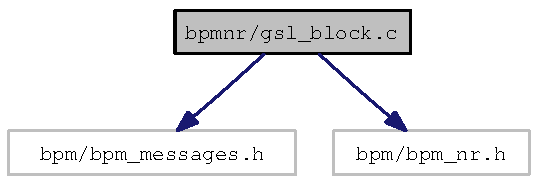
\includegraphics[width=147pt]{gsl__block_8c__incl}
\end{center}
\end{figure}
\subsubsection*{Functions}
\begin{CompactItemize}
\item 
gsl\_\-block $\ast$ {\bf gsl\_\-block\_\-alloc} (const size\_\-t n)
\item 
void \textbf{gsl\_\-block\_\-free} (gsl\_\-block $\ast$b)\label{group__nr_g0952127372c14dce3c3aa65ec0ad9c1e}

\end{CompactItemize}

\subsection{bpmnr/gsl\_\-eigen.c File Reference}
\label{gsl__eigen_8c}\index{bpmnr/gsl\_\-eigen.c@{bpmnr/gsl\_\-eigen.c}}


\subsubsection{Detailed Description}


Definition in file {\bf gsl\_\-eigen.c}.

{\tt \#include $<$bpm/bpm\_\-messages.h$>$}\par
{\tt \#include $<$bpm/bpm\_\-nr.h$>$}\par


Include dependency graph for gsl\_\-eigen.c:\nopagebreak
\begin{figure}[H]
\begin{center}
\leavevmode
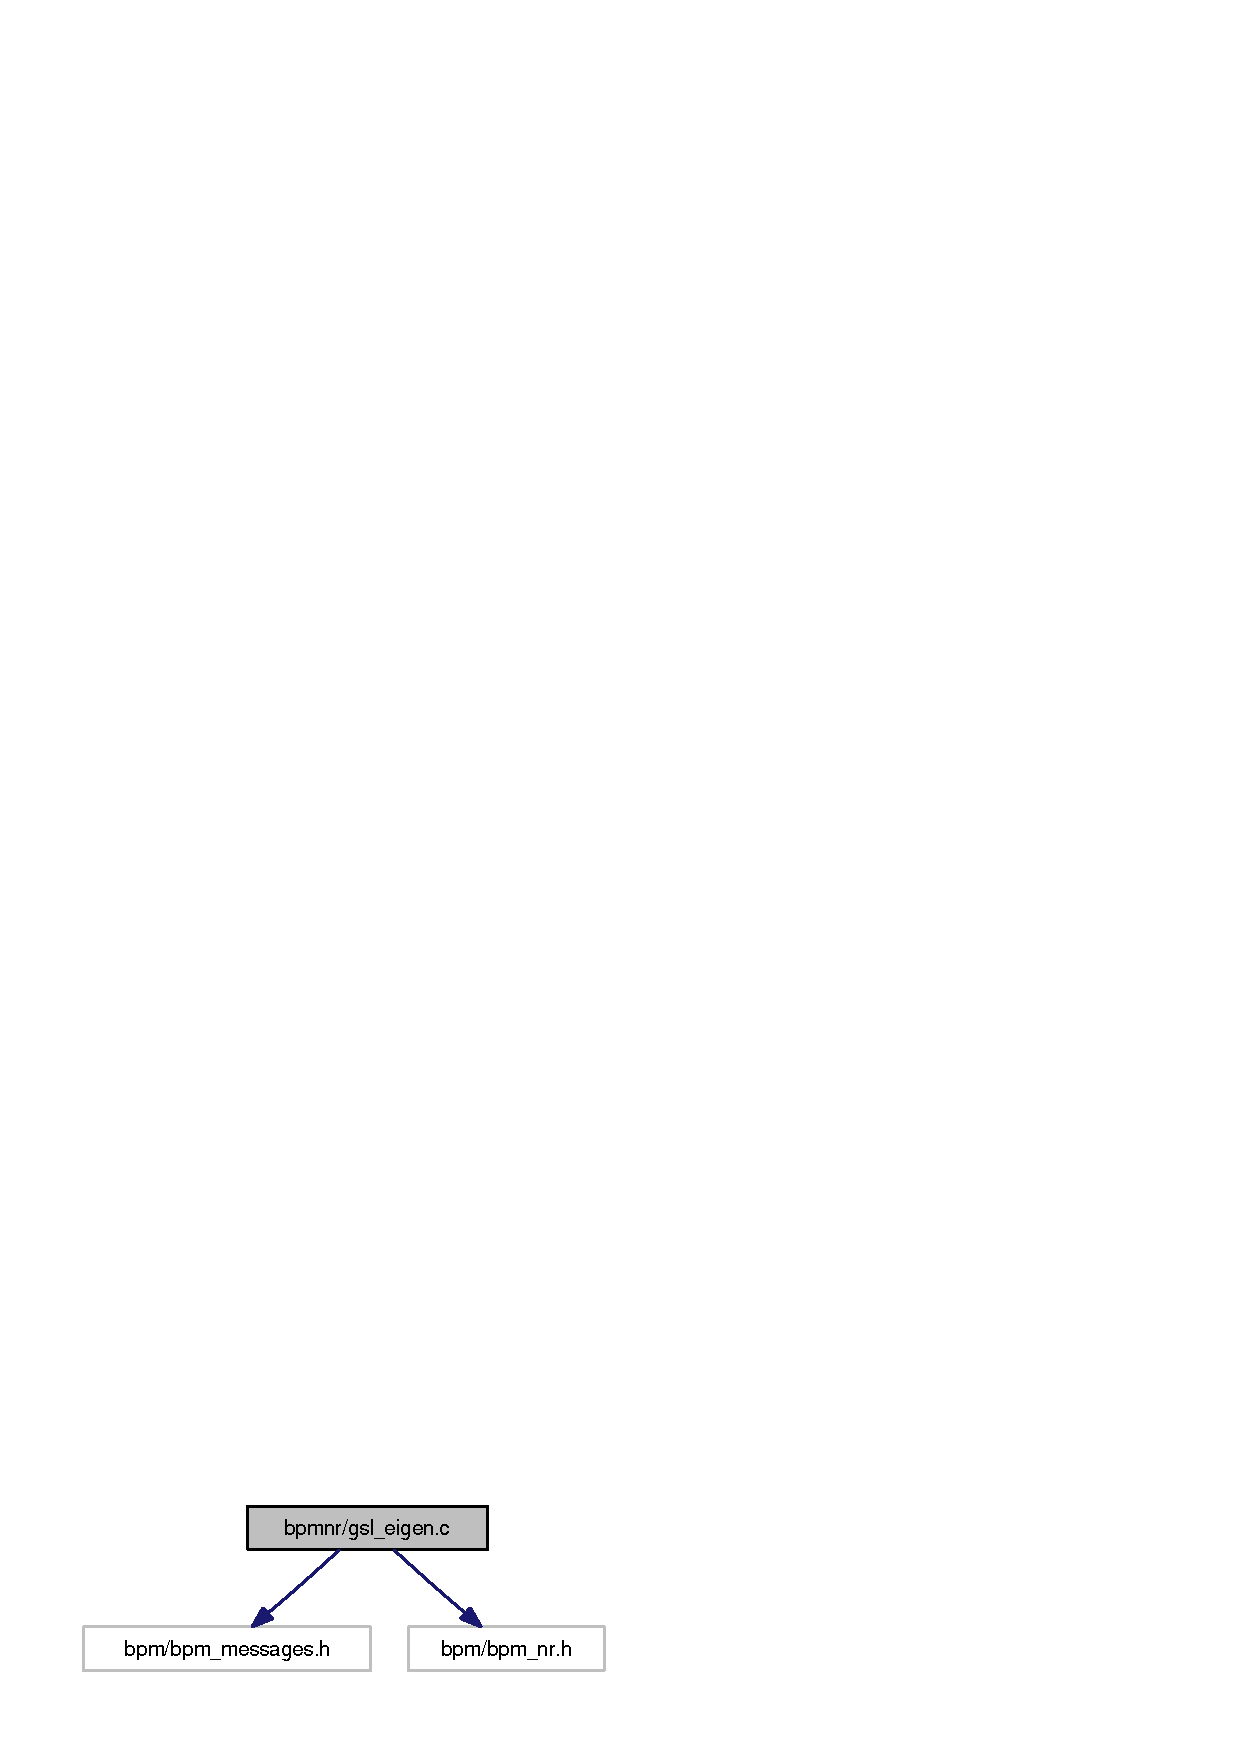
\includegraphics[width=147pt]{gsl__eigen_8c__incl}
\end{center}
\end{figure}
\subsubsection*{Functions}
\begin{CompactItemize}
\item 
void \textbf{chop\_\-small\_\-elements} (gsl\_\-vector $\ast$d, gsl\_\-vector $\ast$f)\label{group__nr_g7a9b4689f2fcd8d6a417a071903df6f1}

\item 
void \textbf{qrstep} (gsl\_\-vector $\ast$d, gsl\_\-vector $\ast$f, gsl\_\-matrix $\ast$U, gsl\_\-matrix $\ast$V)\label{group__nr_g8e5d28fda0cf04d6d70392fa9580c2eb}

\item 
double \textbf{trailing\_\-eigenvalue} (const gsl\_\-vector $\ast$d, const gsl\_\-vector $\ast$f)\label{group__nr_g615603d99ef3bb2a21b32e13761a1474}

\item 
void \textbf{create\_\-schur} (double d0, double f0, double d1, double $\ast$c, double $\ast$s)\label{group__nr_g31a6def59f109d51a7e9af63a8850f0c}

\item 
void \textbf{svd2} (gsl\_\-vector $\ast$d, gsl\_\-vector $\ast$f, gsl\_\-matrix $\ast$U, gsl\_\-matrix $\ast$V)\label{group__nr_ge8a1bf5b51ec0f7ef1e067f01d466033}

\item 
void \textbf{chase\_\-out\_\-intermediate\_\-zero} (gsl\_\-vector $\ast$d, gsl\_\-vector $\ast$f, gsl\_\-matrix $\ast$U, size\_\-t k0)\label{group__nr_g1b67ba06b6b7daa4f73a163f404dd3d7}

\item 
void \textbf{chase\_\-out\_\-trailing\_\-zero} (gsl\_\-vector $\ast$d, gsl\_\-vector $\ast$f, gsl\_\-matrix $\ast$V)\label{group__nr_g15f37e448cf7eabd56ec2c351f148214}

\end{CompactItemize}

\subsection{bpmnr/gsl\_\-linalg.c File Reference}
\label{gsl__linalg_8c}\index{bpmnr/gsl\_\-linalg.c@{bpmnr/gsl\_\-linalg.c}}


\subsubsection{Detailed Description}


Definition in file {\bf gsl\_\-linalg.c}.

{\tt \#include $<$bpm/bpm\_\-messages.h$>$}\par
{\tt \#include $<$bpm/bpm\_\-nr.h$>$}\par


Include dependency graph for gsl\_\-linalg.c:\nopagebreak
\begin{figure}[H]
\begin{center}
\leavevmode
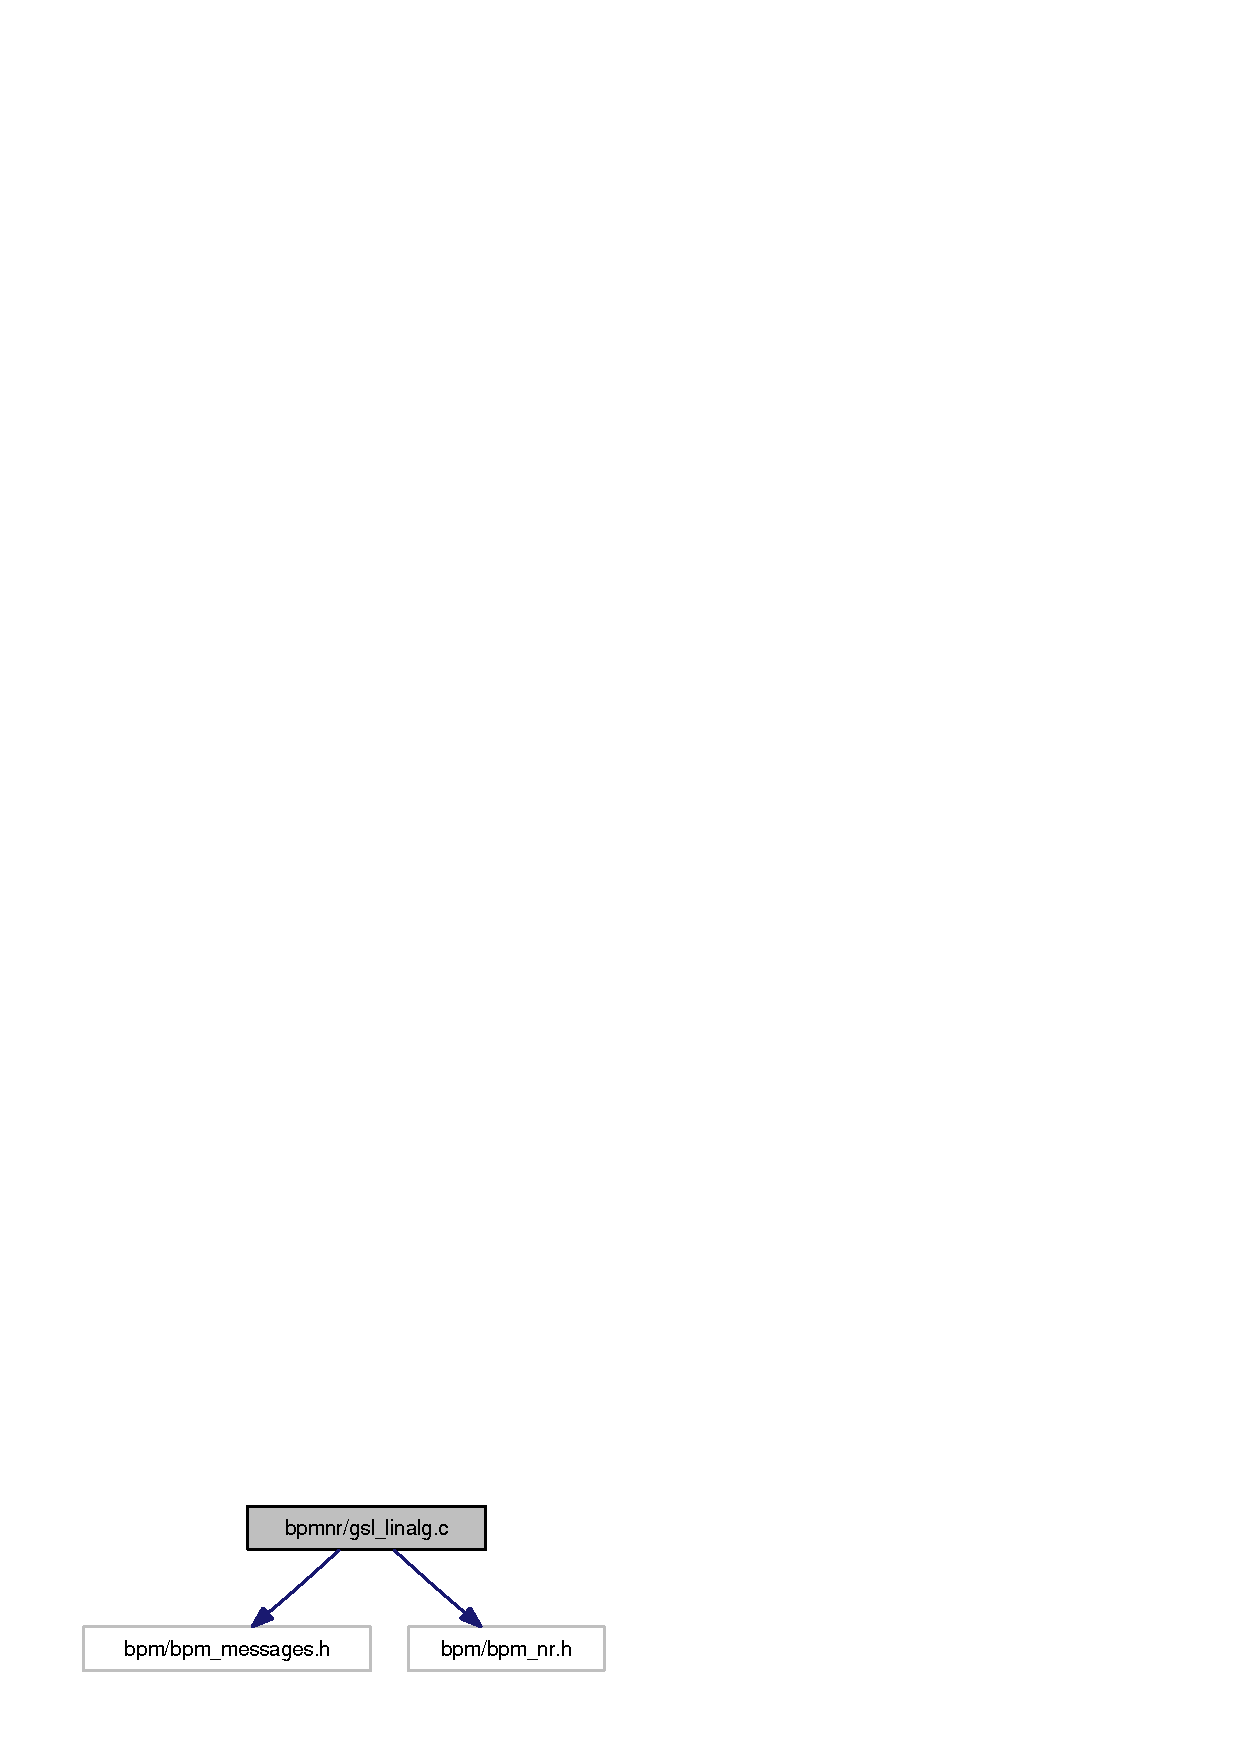
\includegraphics[width=147pt]{gsl__linalg_8c__incl}
\end{center}
\end{figure}
\subsubsection*{Functions}
\begin{CompactItemize}
\item 
int {\bf gsl\_\-linalg\_\-householder\_\-hm} (double tau, const gsl\_\-vector $\ast$v, gsl\_\-matrix $\ast$A)
\item 
int {\bf gsl\_\-linalg\_\-householder\_\-hm1} (double tau, gsl\_\-matrix $\ast$A)
\item 
void \textbf{create\_\-givens} (const double a, const double b, double $\ast$c, double $\ast$s)\label{group__nr_g2c1eb13f0c90da0f8ef4ef712db29f44}

\item 
int \textbf{gsl\_\-linalg\_\-bidiag\_\-decomp} (gsl\_\-matrix $\ast$A, gsl\_\-vector $\ast$tau\_\-U, gsl\_\-vector $\ast$tau\_\-V)\label{gsl__linalg_8c_deb64588fa4ce379603521437cd70eb0}

\item 
double {\bf gsl\_\-linalg\_\-householder\_\-transform} (gsl\_\-vector $\ast$v)
\item 
int {\bf gsl\_\-linalg\_\-householder\_\-mh} (double tau, const gsl\_\-vector $\ast$v, gsl\_\-matrix $\ast$A)
\item 
int \textbf{gsl\_\-linalg\_\-SV\_\-solve} (const gsl\_\-matrix $\ast$U, const gsl\_\-matrix $\ast$V, const gsl\_\-vector $\ast$S, const gsl\_\-vector $\ast$b, gsl\_\-vector $\ast$x)\label{group__nr_g8568eb30743233bab6e1c2d530829f5f}

\item 
int \textbf{gsl\_\-isnan} (const double x)\label{group__nr_gf37b7182e24399515692cc4aa39722dd}

\item 
void \textbf{chop\_\-small\_\-elements} (gsl\_\-vector $\ast$d, gsl\_\-vector $\ast$f)\label{group__nr_g7a9b4689f2fcd8d6a417a071903df6f1}

\item 
void \textbf{qrstep} (gsl\_\-vector $\ast$d, gsl\_\-vector $\ast$f, gsl\_\-matrix $\ast$U, gsl\_\-matrix $\ast$V)\label{group__nr_g8e5d28fda0cf04d6d70392fa9580c2eb}

\item 
double \textbf{trailing\_\-eigenvalue} (const gsl\_\-vector $\ast$d, const gsl\_\-vector $\ast$f)\label{group__nr_g615603d99ef3bb2a21b32e13761a1474}

\item 
void \textbf{create\_\-schur} (double d0, double f0, double d1, double $\ast$c, double $\ast$s)\label{group__nr_g31a6def59f109d51a7e9af63a8850f0c}

\item 
void \textbf{svd2} (gsl\_\-vector $\ast$d, gsl\_\-vector $\ast$f, gsl\_\-matrix $\ast$U, gsl\_\-matrix $\ast$V)\label{group__nr_ge8a1bf5b51ec0f7ef1e067f01d466033}

\item 
void \textbf{chase\_\-out\_\-intermediate\_\-zero} (gsl\_\-vector $\ast$d, gsl\_\-vector $\ast$f, gsl\_\-matrix $\ast$U, size\_\-t k0)\label{group__nr_g1b67ba06b6b7daa4f73a163f404dd3d7}

\item 
void \textbf{chase\_\-out\_\-trailing\_\-zero} (gsl\_\-vector $\ast$d, gsl\_\-vector $\ast$f, gsl\_\-matrix $\ast$V)\label{group__nr_g15f37e448cf7eabd56ec2c351f148214}

\item 
int \textbf{gsl\_\-linalg\_\-bidiag\_\-unpack} (const gsl\_\-matrix $\ast$A, const gsl\_\-vector $\ast$tau\_\-U, gsl\_\-matrix $\ast$U, const gsl\_\-vector $\ast$tau\_\-V, gsl\_\-matrix $\ast$V, gsl\_\-vector $\ast$diag, gsl\_\-vector $\ast$superdiag)\label{group__nr_gc4843a336042d90bbacea983a80e29b9}

\item 
int \textbf{gsl\_\-linalg\_\-bidiag\_\-unpack2} (gsl\_\-matrix $\ast$A, gsl\_\-vector $\ast$tau\_\-U, gsl\_\-vector $\ast$tau\_\-V, gsl\_\-matrix $\ast$V)\label{group__nr_g4881575010a0877aba5efab6f368ab8c}

\item 
int \textbf{gsl\_\-linalg\_\-SV\_\-decomp} (gsl\_\-matrix $\ast$A, gsl\_\-matrix $\ast$V, gsl\_\-vector $\ast$S, gsl\_\-vector $\ast$work)\label{gsl__linalg_8c_1266bf489a94e8360f4e08d3cfdb0903}

\end{CompactItemize}

\subsection{bpmnr/gsl\_\-matrix.c File Reference}
\label{gsl__matrix_8c}\index{bpmnr/gsl\_\-matrix.c@{bpmnr/gsl\_\-matrix.c}}


\subsubsection{Detailed Description}


Definition in file {\bf gsl\_\-matrix.c}.

{\tt \#include $<$bpm/bpm\_\-messages.h$>$}\par
{\tt \#include $<$bpm/bpm\_\-nr.h$>$}\par


Include dependency graph for gsl\_\-matrix.c:\nopagebreak
\begin{figure}[H]
\begin{center}
\leavevmode
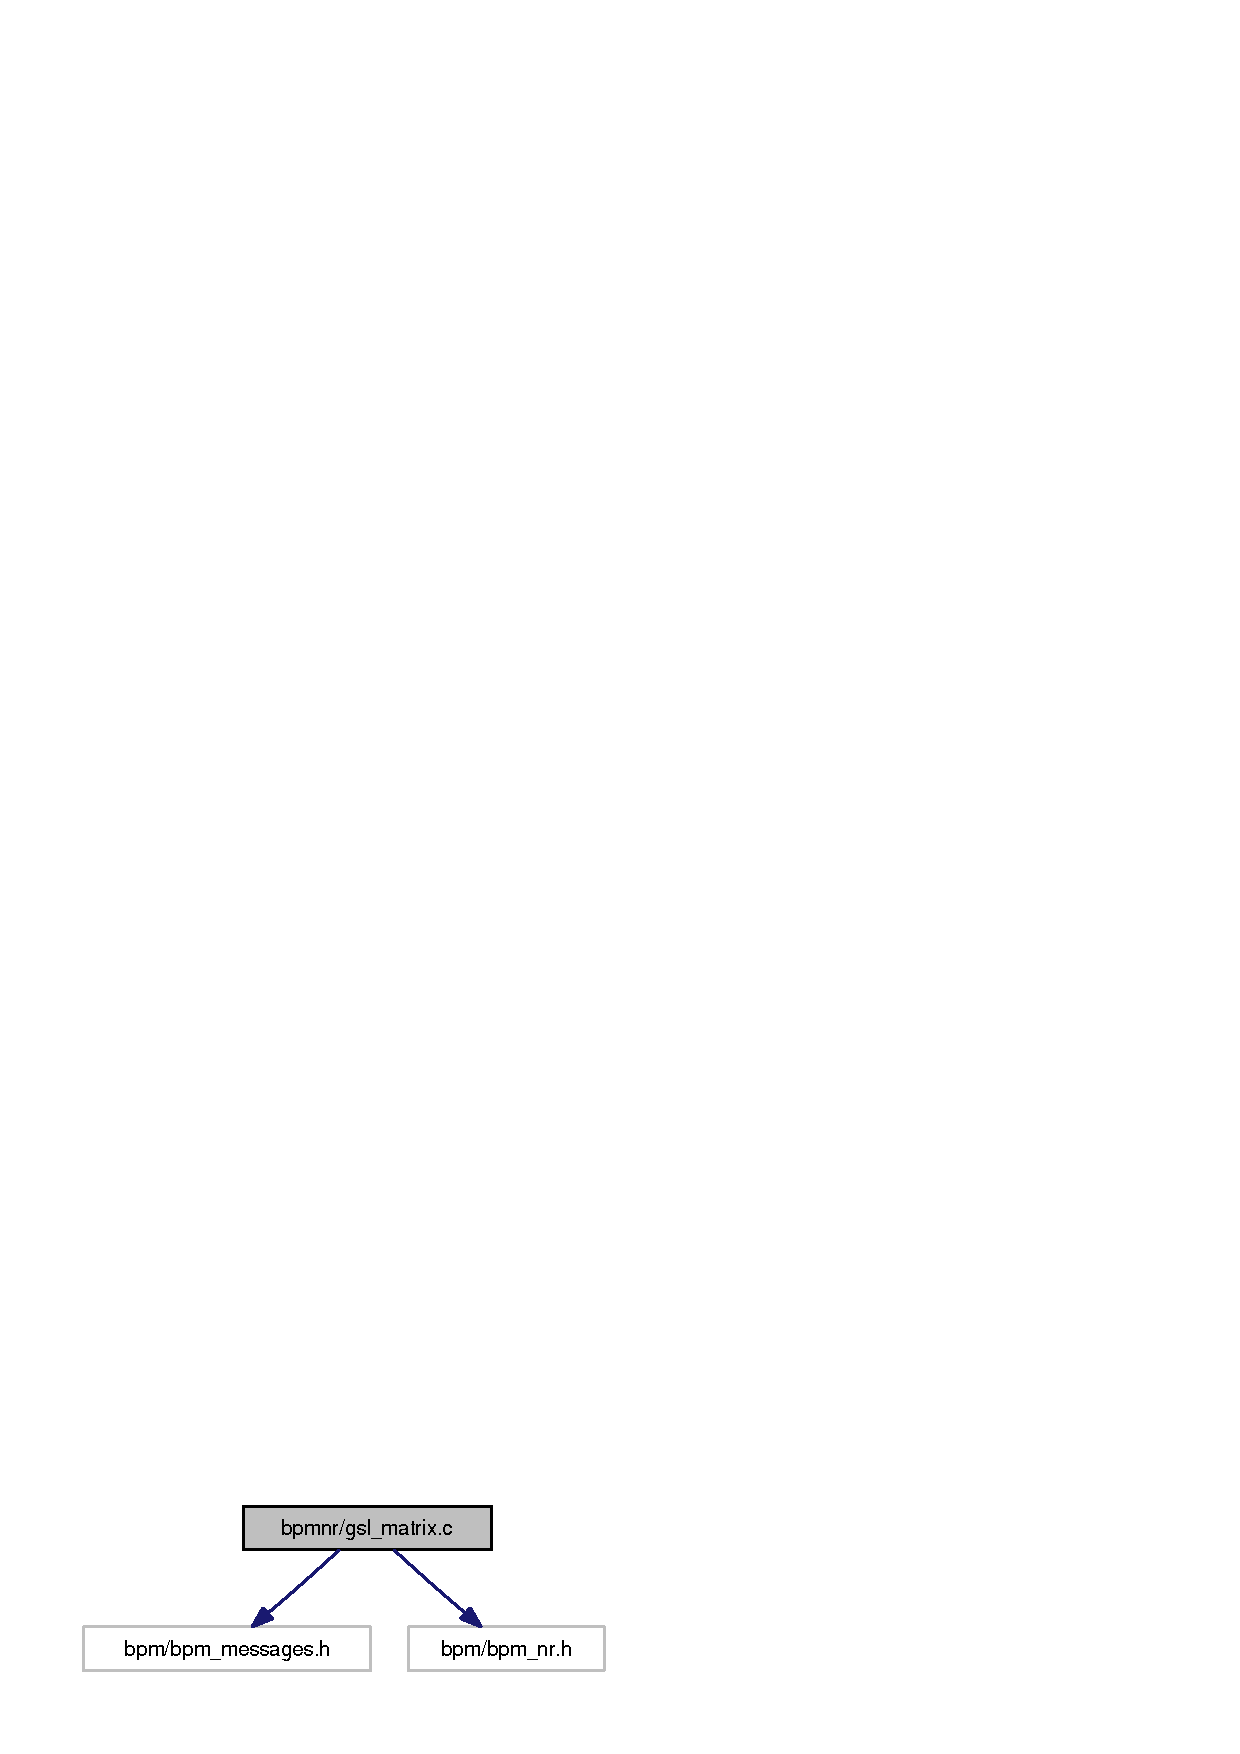
\includegraphics[width=147pt]{gsl__matrix_8c__incl}
\end{center}
\end{figure}
\subsubsection*{Functions}
\begin{CompactItemize}
\item 
int {\bf gsl\_\-matrix\_\-swap\_\-columns} (gsl\_\-matrix $\ast$m, const size\_\-t i, const size\_\-t j)
\item 
\_\-gsl\_\-vector\_\-view {\bf gsl\_\-matrix\_\-column} (gsl\_\-matrix $\ast$m, const size\_\-t j)
\item 
double {\bf gsl\_\-matrix\_\-get} (const gsl\_\-matrix $\ast$m, const size\_\-t i, const size\_\-t j)
\item 
void {\bf gsl\_\-matrix\_\-set} (gsl\_\-matrix $\ast$m, const size\_\-t i, const size\_\-t j, const double x)
\item 
\_\-gsl\_\-matrix\_\-view {\bf gsl\_\-matrix\_\-submatrix} (gsl\_\-matrix $\ast$m, const size\_\-t i, const size\_\-t j, const size\_\-t n1, const size\_\-t n2)
\item 
gsl\_\-matrix $\ast$ \textbf{gsl\_\-matrix\_\-alloc} (const size\_\-t n1, const size\_\-t n2)\label{group__nr_g3c416b23f730c2e06cb5e9b257f1f571}

\item 
gsl\_\-matrix $\ast$ \textbf{gsl\_\-matrix\_\-calloc} (const size\_\-t n1, const size\_\-t n2)\label{group__nr_gf2e18583a2759c9d0f78b564f40eccd7}

\item 
\_\-gsl\_\-vector\_\-const\_\-view \textbf{gsl\_\-matrix\_\-const\_\-row} (const gsl\_\-matrix $\ast$m, const size\_\-t i)\label{group__nr_g1b0f557b9e570f397ab13dcc24e09e35}

\item 
\_\-gsl\_\-vector\_\-view \textbf{gsl\_\-matrix\_\-row} (gsl\_\-matrix $\ast$m, const size\_\-t i)\label{group__nr_gebf16339184d6759f4cdfa9c1724fb98}

\item 
\_\-gsl\_\-vector\_\-const\_\-view \textbf{gsl\_\-matrix\_\-const\_\-column} (const gsl\_\-matrix $\ast$m, const size\_\-t i)\label{group__nr_gf288953bef254a8e2221d778c28f7f97}

\item 
void \textbf{gsl\_\-matrix\_\-set\_\-identity} (gsl\_\-matrix $\ast$m)\label{group__nr_ge37f3f441742e70b1a701d92446e33fc}

\end{CompactItemize}

\subsection{bpmnr/gsl\_\-vector.c File Reference}
\label{gsl__vector_8c}\index{bpmnr/gsl\_\-vector.c@{bpmnr/gsl\_\-vector.c}}


\subsubsection{Detailed Description}


Definition in file {\bf gsl\_\-vector.c}.

{\tt \#include $<$bpm/bpm\_\-messages.h$>$}\par
{\tt \#include $<$bpm/bpm\_\-nr.h$>$}\par


Include dependency graph for gsl\_\-vector.c:\nopagebreak
\begin{figure}[H]
\begin{center}
\leavevmode
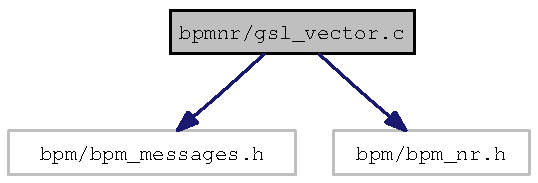
\includegraphics[width=147pt]{gsl__vector_8c__incl}
\end{center}
\end{figure}
\subsubsection*{Functions}
\begin{CompactItemize}
\item 
\_\-gsl\_\-vector\_\-view {\bf gsl\_\-vector\_\-subvector} (gsl\_\-vector $\ast$v, size\_\-t offset, size\_\-t n)
\item 
double {\bf gsl\_\-vector\_\-get} (const gsl\_\-vector $\ast$v, const size\_\-t i)
\item 
void {\bf gsl\_\-vector\_\-set} (gsl\_\-vector $\ast$v, const size\_\-t i, double x)
\item 
int \textbf{gsl\_\-vector\_\-swap\_\-elements} (gsl\_\-vector $\ast$v, const size\_\-t i, const size\_\-t j)\label{group__nr_g2624694e4157398ba344b90eca6ba070}

\item 
gsl\_\-vector $\ast$ \textbf{gsl\_\-vector\_\-alloc} (const size\_\-t n)\label{gsl__vector_8c_af34776639f48fec68e8baab777c6232}

\item 
gsl\_\-vector $\ast$ \textbf{gsl\_\-vector\_\-calloc} (const size\_\-t n)\label{group__nr_gac4c2937f0e28c7a00cfe90b4ad886a6}

\item 
\_\-gsl\_\-vector\_\-const\_\-view \textbf{gsl\_\-vector\_\-const\_\-subvector} (const gsl\_\-vector $\ast$v, size\_\-t offset, size\_\-t n)\label{group__nr_ga45e4b3770af5d15171055314b140838}

\item 
void \textbf{gsl\_\-vector\_\-free} (gsl\_\-vector $\ast$v)\label{group__nr_gedc84887915223f87986de6a67c0249d}

\end{CompactItemize}

\subsection{bpmnr/nr\_\-checks.c File Reference}
\label{nr__checks_8c}\index{bpmnr/nr\_\-checks.c@{bpmnr/nr\_\-checks.c}}


\subsubsection{Detailed Description}


Definition in file {\bf nr\_\-checks.c}.

{\tt \#include $<$bpm/bpm\_\-messages.h$>$}\par
{\tt \#include $<$bpm/bpm\_\-nr.h$>$}\par


Include dependency graph for nr\_\-checks.c:\nopagebreak
\begin{figure}[H]
\begin{center}
\leavevmode
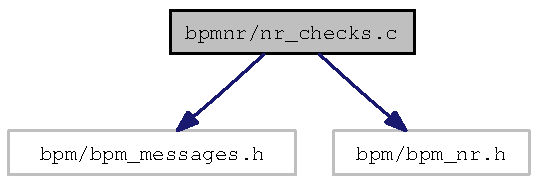
\includegraphics[width=147pt]{nr__checks_8c__incl}
\end{center}
\end{figure}
\subsubsection*{Functions}
\begin{CompactItemize}
\item 
int {\bf nr\_\-is\_\-int} (double x)
\item 
int {\bf nr\_\-is\_\-pow2} (unsigned long n)
\end{CompactItemize}


\subsubsection{Function Documentation}
\index{nr\_\-checks.c@{nr\_\-checks.c}!nr\_\-is\_\-int@{nr\_\-is\_\-int}}
\index{nr\_\-is\_\-int@{nr\_\-is\_\-int}!nr_checks.c@{nr\_\-checks.c}}
\paragraph[nr\_\-is\_\-int]{\setlength{\rightskip}{0pt plus 5cm}int nr\_\-is\_\-int (double {\em x})}\hfill\label{nr__checks_8c_0f1f21216d96e661d4ba6b91e91538ed}


Checks whether the given double is an integer value, handy for doing domain checking to prevent e.g. the function nr\_\-gammln print out \char`\"{}nan\char`\"{} or \char`\"{}inf\char`\"{} values...

For double precision, this check is accurate to 1.0E-323 ... should be enough ;-)

\begin{Desc}
\item[Parameters:]
\begin{description}
\item[{\em x}]floating point argument\end{description}
\end{Desc}
\begin{Desc}
\item[Returns:]TRUE if argument is indeed an integer value, FALSE if not \end{Desc}


Definition at line 21 of file nr\_\-checks.c.

Referenced by nr\_\-gammln().
\subsection{bpmnr/nr\_\-complex.c File Reference}
\label{nr__complex_8c}\index{bpmnr/nr\_\-complex.c@{bpmnr/nr\_\-complex.c}}


\subsubsection{Detailed Description}


Definition in file {\bf nr\_\-complex.c}.

{\tt \#include \char`\"{}bpm/bpm\_\-nr.h\char`\"{}}\par


Include dependency graph for nr\_\-complex.c:\nopagebreak
\begin{figure}[H]
\begin{center}
\leavevmode
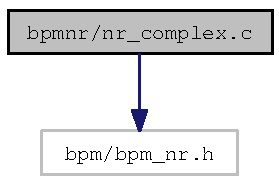
\includegraphics[width=85pt]{nr__complex_8c__incl}
\end{center}
\end{figure}
\subsubsection*{Functions}
\begin{CompactItemize}
\item 
{\bf complex\_\-t} \textbf{complex} (double re, double im)\label{group__nr_g203888bac468229094352b2bb9456417}

\item 
double \textbf{c\_\-real} ({\bf complex\_\-t} z)\label{group__nr_gbd9dcd9992cad1f6af326811da66fc9a}

\item 
double \textbf{c\_\-imag} ({\bf complex\_\-t} z)\label{group__nr_g6adc8ee3a56fe88de97c3f40c484f824}

\item 
double \textbf{c\_\-abs} ({\bf complex\_\-t} z)\label{group__nr_gdd54790aa13824ee1db3d0558a465071}

\item 
double \textbf{c\_\-abs2} ({\bf complex\_\-t} z)\label{group__nr_g5a31b290dd721358e4270d9686347dde}

\item 
double \textbf{c\_\-arg} ({\bf complex\_\-t} z)\label{group__nr_g5a8776cef7d6ef88a11015d6ec2665ba}

\item 
{\bf complex\_\-t} \textbf{c\_\-conj} ({\bf complex\_\-t} z)\label{group__nr_g26f4378875ac801b1b5bb7a13f180f0a}

\item 
{\bf complex\_\-t} \textbf{c\_\-neg} ({\bf complex\_\-t} z)\label{group__nr_g33f198bcc4dd193c4f8c8db9049311d2}

\item 
{\bf complex\_\-t} \textbf{c\_\-sum} ({\bf complex\_\-t} z1, {\bf complex\_\-t} z2)\label{group__nr_g176d351f4b035de54e1fb9974c296bed}

\item 
{\bf complex\_\-t} \textbf{c\_\-diff} ({\bf complex\_\-t} z1, {\bf complex\_\-t} z2)\label{group__nr_g5b48402b525952efb744f5b2804d1957}

\item 
{\bf complex\_\-t} \textbf{c\_\-mult} ({\bf complex\_\-t} z1, {\bf complex\_\-t} z2)\label{group__nr_gbac492f503bff737e6a11c03e44e7ada}

\item 
{\bf complex\_\-t} \textbf{c\_\-scale} (double r, {\bf complex\_\-t} z)\label{group__nr_g4a8c814a8cb7b92c919b23e1ea64d615}

\item 
{\bf complex\_\-t} \textbf{c\_\-div} ({\bf complex\_\-t} z1, {\bf complex\_\-t} z2)\label{group__nr_g3cb3d7ddec167a30a5f7a159dea26c0f}

\item 
{\bf complex\_\-t} \textbf{c\_\-sqr} ({\bf complex\_\-t} z)\label{group__nr_g72516630e1d745f5d1630b4c525cb5f8}

\item 
double \textbf{c\_\-norm2} ({\bf complex\_\-t} z)\label{group__nr_g98f394b1ddccfeb4d9b5edb6c1f8c652}

\item 
{\bf complex\_\-t} \textbf{c\_\-exp} ({\bf complex\_\-t} z)\label{group__nr_g41a40da9e1d42de8e76d999abd476f8a}

\item 
{\bf complex\_\-t} \textbf{c\_\-sqrt} ({\bf complex\_\-t} z)\label{group__nr_g22d2bd8775120d34e3b700682e67d955}

\item 
int \textbf{c\_\-isequal} ({\bf complex\_\-t} z1, {\bf complex\_\-t} z2)\label{group__nr_gd3e4d63450915ff27b8e506acb21bb2e}

\end{CompactItemize}

\subsection{bpmnr/nr\_\-fit.c File Reference}
\label{nr__fit_8c}\index{bpmnr/nr\_\-fit.c@{bpmnr/nr\_\-fit.c}}


\subsubsection{Detailed Description}


Definition in file {\bf nr\_\-fit.c}.

{\tt \#include $<$bpm/bpm\_\-messages.h$>$}\par
{\tt \#include $<$bpm/bpm\_\-nr.h$>$}\par


Include dependency graph for nr\_\-fit.c:\nopagebreak
\begin{figure}[H]
\begin{center}
\leavevmode
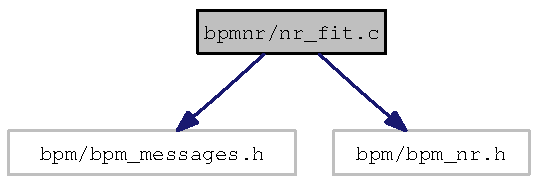
\includegraphics[width=147pt]{nr__fit_8c__incl}
\end{center}
\end{figure}
\subsubsection*{Functions}
\begin{CompactItemize}
\item 
int {\bf nr\_\-fit} (double $\ast$x, double y[$\,$], int ndata, double sig[$\,$], int mwt, double $\ast$a, double $\ast$b, double $\ast$siga, double $\ast$sigb, double $\ast$chi2, double $\ast$q)
\end{CompactItemize}

\subsection{bpmnr/nr\_\-four1.c File Reference}
\label{nr__four1_8c}\index{bpmnr/nr\_\-four1.c@{bpmnr/nr\_\-four1.c}}


\subsubsection{Detailed Description}


Definition in file {\bf nr\_\-four1.c}.

{\tt \#include $<$bpm/bpm\_\-messages.h$>$}\par
{\tt \#include $<$bpm/bpm\_\-nr.h$>$}\par


Include dependency graph for nr\_\-four1.c:\nopagebreak
\begin{figure}[H]
\begin{center}
\leavevmode
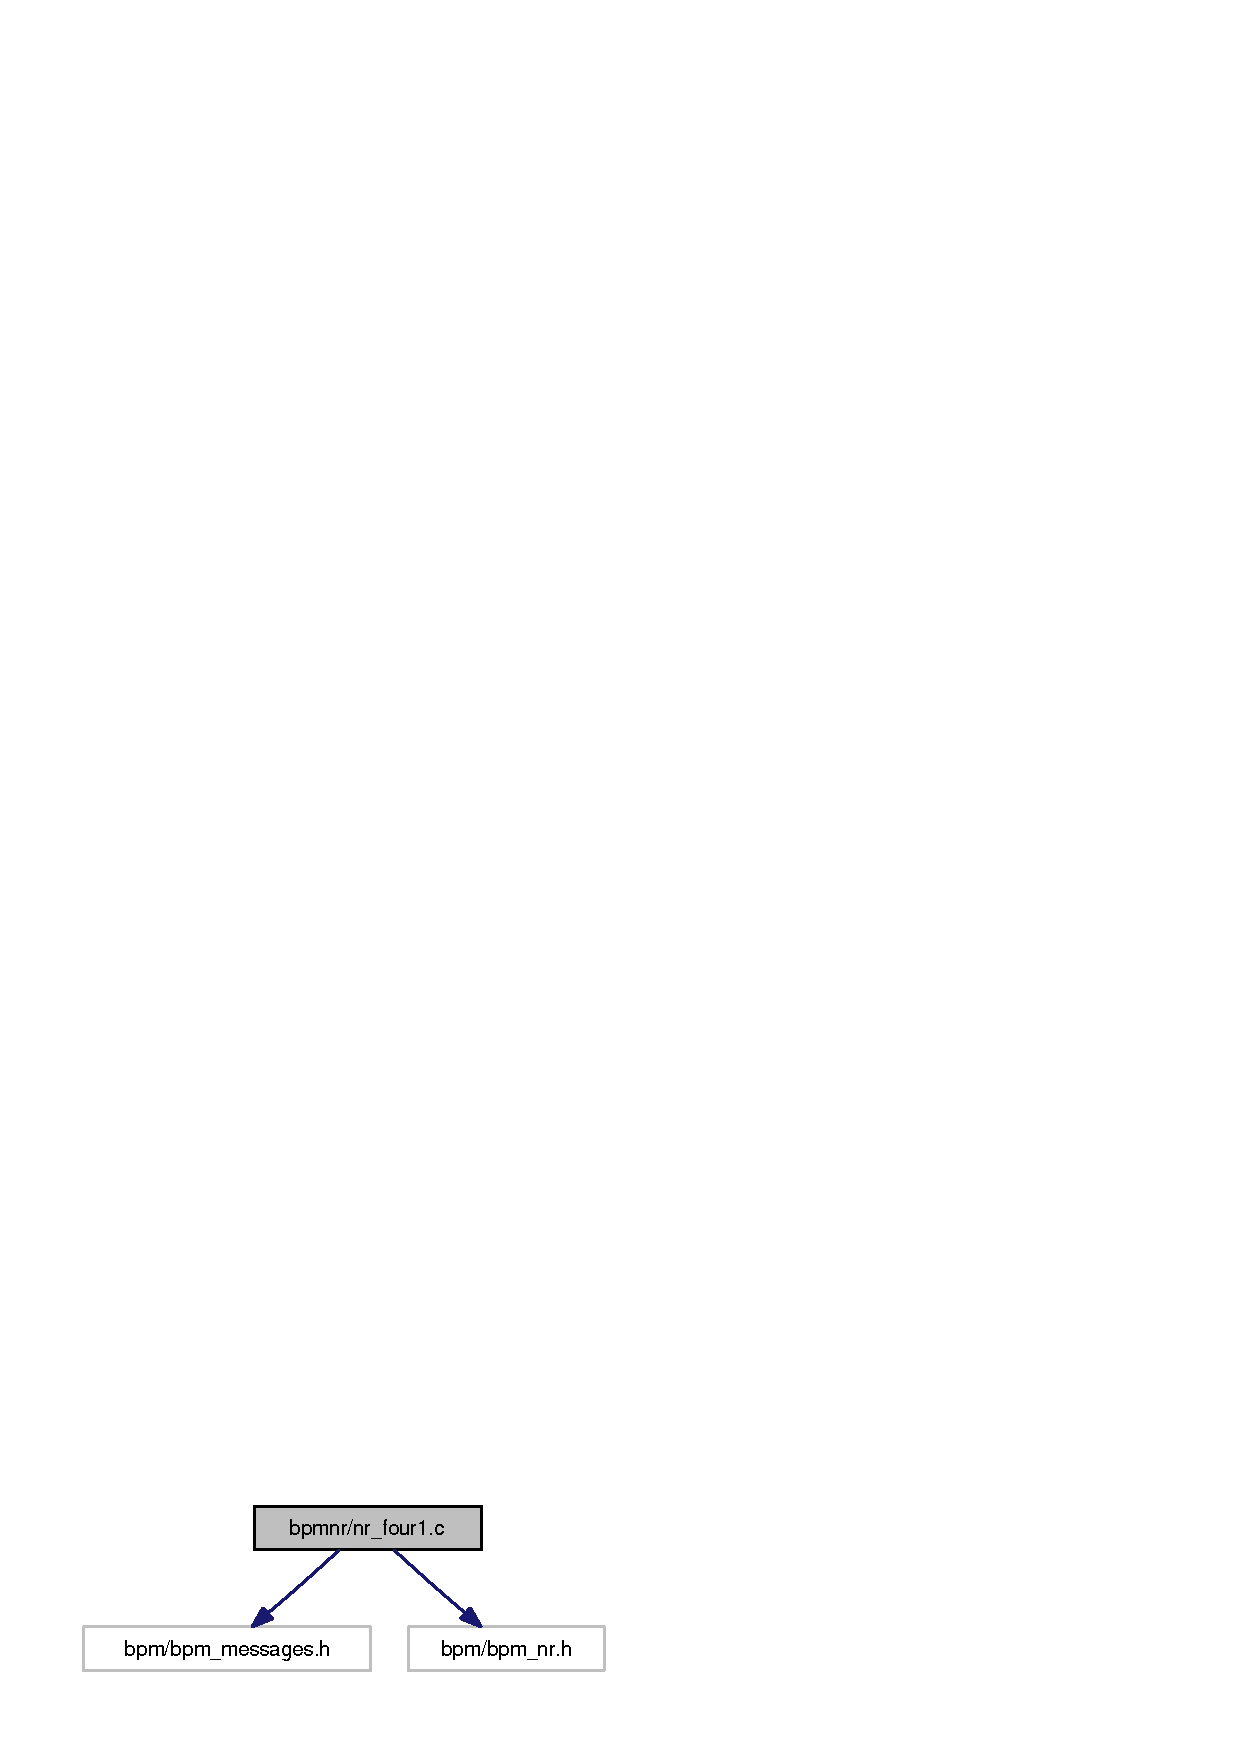
\includegraphics[width=147pt]{nr__four1_8c__incl}
\end{center}
\end{figure}
\subsubsection*{Functions}
\begin{CompactItemize}
\item 
int {\bf nr\_\-four1} (double data[$\,$], unsigned long nn, int isign)
\end{CompactItemize}

\subsection{bpmnr/nr\_\-gammln.c File Reference}
\label{nr__gammln_8c}\index{bpmnr/nr\_\-gammln.c@{bpmnr/nr\_\-gammln.c}}


\subsubsection{Detailed Description}


Definition in file {\bf nr\_\-gammln.c}.

{\tt \#include $<$bpm/bpm\_\-messages.h$>$}\par
{\tt \#include $<$bpm/bpm\_\-nr.h$>$}\par


Include dependency graph for nr\_\-gammln.c:\nopagebreak
\begin{figure}[H]
\begin{center}
\leavevmode
\includegraphics[width=147pt]{nr__gammln_8c__incl}
\end{center}
\end{figure}
\subsubsection*{Functions}
\begin{CompactItemize}
\item 
double {\bf nr\_\-gammln} (double xx)
\end{CompactItemize}

\subsection{bpmnr/nr\_\-gammq.c File Reference}
\label{nr__gammq_8c}\index{bpmnr/nr\_\-gammq.c@{bpmnr/nr\_\-gammq.c}}


\subsubsection{Detailed Description}


Definition in file {\bf nr\_\-gammq.c}.

{\tt \#include $<$bpm/bpm\_\-messages.h$>$}\par
{\tt \#include $<$bpm/bpm\_\-nr.h$>$}\par


Include dependency graph for nr\_\-gammq.c:\nopagebreak
\begin{figure}[H]
\begin{center}
\leavevmode
\includegraphics[width=147pt]{nr__gammq_8c__incl}
\end{center}
\end{figure}
\subsubsection*{Functions}
\begin{CompactItemize}
\item 
double {\bf nr\_\-gammq} (double a, double x)
\end{CompactItemize}

\subsection{bpmnr/nr\_\-gcf.c File Reference}
\label{nr__gcf_8c}\index{bpmnr/nr\_\-gcf.c@{bpmnr/nr\_\-gcf.c}}


\subsubsection{Detailed Description}


Definition in file {\bf nr\_\-gcf.c}.

{\tt \#include $<$bpm/bpm\_\-messages.h$>$}\par
{\tt \#include $<$bpm/bpm\_\-nr.h$>$}\par


Include dependency graph for nr\_\-gcf.c:\nopagebreak
\begin{figure}[H]
\begin{center}
\leavevmode
\includegraphics[width=147pt]{nr__gcf_8c__incl}
\end{center}
\end{figure}
\subsubsection*{Functions}
\begin{CompactItemize}
\item 
int {\bf nr\_\-gcf} (double $\ast$gammcf, double a, double x, double $\ast$gln)
\end{CompactItemize}

\subsection{bpmnr/nr\_\-gser.c File Reference}
\label{nr__gser_8c}\index{bpmnr/nr\_\-gser.c@{bpmnr/nr\_\-gser.c}}


\subsubsection{Detailed Description}


Definition in file {\bf nr\_\-gser.c}.

{\tt \#include $<$bpm/bpm\_\-messages.h$>$}\par
{\tt \#include $<$bpm/bpm\_\-nr.h$>$}\par


Include dependency graph for nr\_\-gser.c:\nopagebreak
\begin{figure}[H]
\begin{center}
\leavevmode
\includegraphics[width=147pt]{nr__gser_8c__incl}
\end{center}
\end{figure}
\subsubsection*{Functions}
\begin{CompactItemize}
\item 
int {\bf nr\_\-gser} (double $\ast$gamser, double a, double x, double $\ast$gln)
\end{CompactItemize}

\subsection{bpmnr/nr\_\-levmar.c File Reference}
\label{nr__levmar_8c}\index{bpmnr/nr\_\-levmar.c@{bpmnr/nr\_\-levmar.c}}


\subsubsection{Detailed Description}
These routines have been written by : and were released under GPL

Manolis Lourakis Institute of Computer Science, Foundation for Research and Technology - Hellas, Heraklion, Crete, Greece

//////////////////////////////////////////////////////////////////////////////

Levenberg - Marquardt non-linear minimization algorithm Copyright (C) 2004 Manolis Lourakis ({\tt lourakis@ics.forth.gr}) Institute of Computer Science, Foundation for Research \& Technology - Hellas Heraklion, Crete, Greece.

This program is free software; you can redistribute it and/or modify it under the terms of the GNU General Public License as published by the Free Software Foundation; either version 2 of the License, or (at your option) any later version.

This program is distributed in the hope that it will be useful, but WITHOUT ANY WARRANTY; without even the implied warranty of MERCHANTABILITY or FITNESS FOR A PARTICULAR PURPOSE. See the GNU General Public License for more details.

//////////////////////////////////////////////////////////////////////////////

Changes: BM. Modified the names of the routines somewhat to have them correspond to the rest of libbpm 

Definition in file {\bf nr\_\-levmar.c}.

{\tt \#include $<$bpm/bpm\_\-messages.h$>$}\par
{\tt \#include $<$bpm/bpm\_\-nr.h$>$}\par


Include dependency graph for nr\_\-levmar.c:\nopagebreak
\begin{figure}[H]
\begin{center}
\leavevmode
\includegraphics[width=147pt]{nr__levmar_8c__incl}
\end{center}
\end{figure}
\subsubsection*{Defines}
\begin{CompactItemize}
\item 
\#define \textbf{\_\-\_\-MIN\_\-\_\-}(x, y)\label{nr__levmar_8c_dd73ec9a0a73a097f8b71a96880aee73}

\item 
\#define \textbf{\_\-\_\-MAX\_\-\_\-}(x, y)\label{nr__levmar_8c_d2fc73ab898a3b72dda204a835aad51b}

\end{CompactItemize}
\subsubsection*{Functions}
\begin{CompactItemize}
\item 
void \textbf{nr\_\-trans\_\-mat\_\-mat\_\-mult} (double $\ast$a, double $\ast$b, int n, int m)\label{group__nr_gb647cf24b2b6ab2a0dd993ba4021447c}

\item 
void \textbf{nr\_\-fdif\_\-forw\_\-jac\_\-approx} (void($\ast$func)(double $\ast$p, double $\ast$hx, int m, int n, void $\ast$adata), double $\ast$p, double $\ast$hx, double $\ast$hxx, double delta, double $\ast$jac, int m, int n, void $\ast$adata)\label{group__nr_gf20223185cc5c2a215cb6559231dd55b}

\item 
void \textbf{nr\_\-fdif\_\-cent\_\-jac\_\-approx} (void($\ast$func)(double $\ast$p, double $\ast$hx, int m, int n, void $\ast$adata), double $\ast$p, double $\ast$hxm, double $\ast$hxp, double delta, double $\ast$jac, int m, int n, void $\ast$adata)\label{group__nr_geab4b93cc9d2f74f4c1859204fc9e694}

\item 
void \textbf{nr\_\-lmchkjac} (void($\ast$func)(double $\ast$p, double $\ast$hx, int m, int n, void $\ast$adata), void($\ast$jacf)(double $\ast$p, double $\ast$j, int m, int n, void $\ast$adata), double $\ast$p, int m, int n, void $\ast$adata, double $\ast$err)\label{group__nr_gc0c5d8dc11fc35234e751fbc54a6a185}

\item 
int \textbf{nr\_\-lmcovar} (double $\ast$JtJ, double $\ast$C, double sumsq, int m, int n)\label{group__nr_g2e38d1d3a33b269e190fb0edd3fc3303}

\item 
int \textbf{nr\_\-lmder} (void($\ast$func)(double $\ast$p, double $\ast$hx, int m, int n, void $\ast$adata), void($\ast$jacf)(double $\ast$p, double $\ast$j, int m, int n, void $\ast$adata), double $\ast$p, double $\ast$x, int m, int n, int itmax, double opts[4], double info[LM\_\-INFO\_\-SZ], double $\ast$work, double $\ast$covar, void $\ast$adata)\label{nr__levmar_8c_4e3627752472ab793c8c484b1a69c87e}

\item 
int \textbf{nr\_\-lmdif} (void($\ast$func)(double $\ast$p, double $\ast$hx, int m, int n, void $\ast$adata), double $\ast$p, double $\ast$x, int m, int n, int itmax, double opts[5], double info[LM\_\-INFO\_\-SZ], double $\ast$work, double $\ast$covar, void $\ast$adata)\label{nr__levmar_8c_70e64815dc077832e55d0e97747f3a2d}

\item 
int \textbf{nr\_\-ax\_\-eq\_\-b\_\-LU} (double $\ast$A, double $\ast$B, double $\ast$x, int m)\label{group__nr_g50388d5d50f760129a054ea526ed1c07}

\item 
int \textbf{nr\_\-lmder\_\-bc} (void($\ast$func)(double $\ast$p, double $\ast$hx, int m, int n, void $\ast$adata), void($\ast$jacf)(double $\ast$p, double $\ast$j, int m, int n, void $\ast$adata), double $\ast$p, double $\ast$x, int m, int n, double $\ast$lb, double $\ast$ub, int itmax, double opts[4], double info[LM\_\-INFO\_\-SZ], double $\ast$work, double $\ast$covar, void $\ast$adata)\label{nr__levmar_8c_1a6631bd454e7f929d3d6f050d090f48}

\item 
void \textbf{lmbc\_\-dif\_\-func} (double $\ast$p, double $\ast$hx, int m, int n, void $\ast$data)\label{nr__levmar_8c_353a1c2f31d7a4ba23bf49de06f11887}

\item 
void \textbf{lmbc\_\-dif\_\-jacf} (double $\ast$p, double $\ast$jac, int m, int n, void $\ast$data)\label{nr__levmar_8c_afc1acb2a7b662755edf7b0cb0985e75}

\item 
int \textbf{nr\_\-lmdif\_\-bc} (void($\ast$func)(double $\ast$p, double $\ast$hx, int m, int n, void $\ast$adata), double $\ast$p, double $\ast$x, int m, int n, double $\ast$lb, double $\ast$ub, int itmax, double opts[5], double info[LM\_\-INFO\_\-SZ], double $\ast$work, double $\ast$covar, void $\ast$adata)\label{nr__levmar_8c_5218f124b704f39964d9c12592e7f629}

\end{CompactItemize}

\subsection{bpmnr/nr\_\-median.c File Reference}
\label{nr__median_8c}\index{bpmnr/nr\_\-median.c@{bpmnr/nr\_\-median.c}}


\subsubsection{Detailed Description}


Definition in file {\bf nr\_\-median.c}.

{\tt \#include $<$bpm/bpm\_\-messages.h$>$}\par
{\tt \#include $<$bpm/bpm\_\-nr.h$>$}\par


Include dependency graph for nr\_\-median.c:\nopagebreak
\begin{figure}[H]
\begin{center}
\leavevmode
\includegraphics[width=147pt]{nr__median_8c__incl}
\end{center}
\end{figure}
\subsubsection*{Functions}
\begin{CompactItemize}
\item 
double {\bf nr\_\-median} (int n, double $\ast$arr)
\end{CompactItemize}

\subsection{bpmnr/nr\_\-quadinterpol.c File Reference}
\label{nr__quadinterpol_8c}\index{bpmnr/nr\_\-quadinterpol.c@{bpmnr/nr\_\-quadinterpol.c}}


\subsubsection{Detailed Description}


Definition in file {\bf nr\_\-quadinterpol.c}.

{\tt \#include \char`\"{}bpm\_\-nr.h\char`\"{}}\par


Include dependency graph for nr\_\-quadinterpol.c:\nopagebreak
\begin{figure}[H]
\begin{center}
\leavevmode
\includegraphics[width=253pt]{nr__quadinterpol_8c__incl}
\end{center}
\end{figure}
\subsubsection*{Functions}
\begin{CompactItemize}
\item 
double {\bf nr\_\-quadinterpol} (double x, double x1, double x2, double x3, double y1, double y2, double y3)
\end{CompactItemize}

\subsection{bpmnr/nr\_\-ran1.c File Reference}
\label{nr__ran1_8c}\index{bpmnr/nr\_\-ran1.c@{bpmnr/nr\_\-ran1.c}}


\subsubsection{Detailed Description}


Definition in file {\bf nr\_\-ran1.c}.

{\tt \#include $<$bpm/bpm\_\-nr.h$>$}\par


Include dependency graph for nr\_\-ran1.c:\nopagebreak
\begin{figure}[H]
\begin{center}
\leavevmode
\includegraphics[width=74pt]{nr__ran1_8c__incl}
\end{center}
\end{figure}
\subsubsection*{Functions}
\begin{CompactItemize}
\item 
double {\bf nr\_\-ran1} (long $\ast$idum)
\end{CompactItemize}

\subsection{bpmnr/nr\_\-rangauss.c File Reference}
\label{nr__rangauss_8c}\index{bpmnr/nr\_\-rangauss.c@{bpmnr/nr\_\-rangauss.c}}


\subsubsection{Detailed Description}


Definition in file {\bf nr\_\-rangauss.c}.

{\tt \#include $<$stdio.h$>$}\par
{\tt \#include $<$bpm/bpm\_\-messages.h$>$}\par
{\tt \#include $<$bpm/bpm\_\-nr.h$>$}\par


Include dependency graph for nr\_\-rangauss.c:\nopagebreak
\begin{figure}[H]
\begin{center}
\leavevmode
\includegraphics[width=182pt]{nr__rangauss_8c__incl}
\end{center}
\end{figure}
\subsubsection*{Functions}
\begin{CompactItemize}
\item 
double {\bf nr\_\-rangauss} (double mean, double std\_\-dev)
\end{CompactItemize}

\subsection{bpmnr/nr\_\-ranuniform.c File Reference}
\label{nr__ranuniform_8c}\index{bpmnr/nr\_\-ranuniform.c@{bpmnr/nr\_\-ranuniform.c}}


\subsubsection{Detailed Description}


Definition in file {\bf nr\_\-ranuniform.c}.

{\tt \#include $<$bpm/bpm\_\-messages.h$>$}\par
{\tt \#include $<$bpm/bpm\_\-nr.h$>$}\par


Include dependency graph for nr\_\-ranuniform.c:\nopagebreak
\begin{figure}[H]
\begin{center}
\leavevmode
\includegraphics[width=147pt]{nr__ranuniform_8c__incl}
\end{center}
\end{figure}
\subsubsection*{Functions}
\begin{CompactItemize}
\item 
double {\bf nr\_\-ranuniform} (double lower, double upper)
\end{CompactItemize}

\subsection{bpmnr/nr\_\-realft.c File Reference}
\label{nr__realft_8c}\index{bpmnr/nr\_\-realft.c@{bpmnr/nr\_\-realft.c}}


\subsubsection{Detailed Description}


Definition in file {\bf nr\_\-realft.c}.

{\tt \#include $<$bpm/bpm\_\-messages.h$>$}\par
{\tt \#include $<$bpm/bpm\_\-nr.h$>$}\par


Include dependency graph for nr\_\-realft.c:\nopagebreak
\begin{figure}[H]
\begin{center}
\leavevmode
\includegraphics[width=147pt]{nr__realft_8c__incl}
\end{center}
\end{figure}
\subsubsection*{Functions}
\begin{CompactItemize}
\item 
int {\bf nr\_\-realft} (double data[$\,$], unsigned long n, int isign)
\end{CompactItemize}

\subsection{bpmnr/nr\_\-seed.c File Reference}
\label{nr__seed_8c}\index{bpmnr/nr\_\-seed.c@{bpmnr/nr\_\-seed.c}}


\subsubsection{Detailed Description}


Definition in file {\bf nr\_\-seed.c}.

{\tt \#include $<$bpm/bpm\_\-messages.h$>$}\par
{\tt \#include $<$bpm/bpm\_\-nr.h$>$}\par


Include dependency graph for nr\_\-seed.c:\nopagebreak
\begin{figure}[H]
\begin{center}
\leavevmode
\includegraphics[width=147pt]{nr__seed_8c__incl}
\end{center}
\end{figure}
\subsubsection*{Functions}
\begin{CompactItemize}
\item 
int {\bf nr\_\-seed} (long seed)
\end{CompactItemize}
\subsubsection*{Variables}
\begin{CompactItemize}
\item 
long {\bf bpm\_\-rseed}
\end{CompactItemize}


\subsubsection{Variable Documentation}
\index{nr\_\-seed.c@{nr\_\-seed.c}!bpm\_\-rseed@{bpm\_\-rseed}}
\index{bpm\_\-rseed@{bpm\_\-rseed}!nr_seed.c@{nr\_\-seed.c}}
\paragraph[bpm\_\-rseed]{\setlength{\rightskip}{0pt plus 5cm}long {\bf bpm\_\-rseed}}\hfill\label{nr__seed_8c_c988f9e1a0efc51f61aa8731b011a44b}


the global random seed variable 

Definition at line 9 of file nr\_\-seed.c.

Referenced by nr\_\-rangauss(), nr\_\-ranuniform(), and nr\_\-seed().
\subsection{bpmnr/nr\_\-select.c File Reference}
\label{nr__select_8c}\index{bpmnr/nr\_\-select.c@{bpmnr/nr\_\-select.c}}


\subsubsection{Detailed Description}


Definition in file {\bf nr\_\-select.c}.

{\tt \#include $<$bpm/bpm\_\-messages.h$>$}\par
{\tt \#include $<$bpm/bpm\_\-nr.h$>$}\par


Include dependency graph for nr\_\-select.c:\nopagebreak
\begin{figure}[H]
\begin{center}
\leavevmode
\includegraphics[width=147pt]{nr__select_8c__incl}
\end{center}
\end{figure}
\subsubsection*{Functions}
\begin{CompactItemize}
\item 
double {\bf nr\_\-select} (int k, int n, double $\ast$org\_\-arr)
\end{CompactItemize}

\subsection{bpmnr/nr\_\-sinc.c File Reference}
\label{nr__sinc_8c}\index{bpmnr/nr\_\-sinc.c@{bpmnr/nr\_\-sinc.c}}


\subsubsection{Detailed Description}


Definition in file {\bf nr\_\-sinc.c}.

{\tt \#include \char`\"{}bpm\_\-nr.h\char`\"{}}\par


Include dependency graph for nr\_\-sinc.c:\nopagebreak
\begin{figure}[H]
\begin{center}
\leavevmode
\includegraphics[width=253pt]{nr__sinc_8c__incl}
\end{center}
\end{figure}
\subsubsection*{Functions}
\begin{CompactItemize}
\item 
double {\bf sinc} (double x)
\item 
double {\bf lanczos} (double x, int a)
\end{CompactItemize}

\subsection{bpmorbit/bpm\_\-orbit.h File Reference}
\label{bpm__orbit_8h}\index{bpmorbit/bpm\_\-orbit.h@{bpmorbit/bpm\_\-orbit.h}}


\subsubsection{Detailed Description}
libbpm orbit generation routines 

This header contains beam oribit generation routines, so this includes also calibration scans etc... 

Definition in file {\bf bpm\_\-orbit.h}.

{\tt \#include $<$math.h$>$}\par
{\tt \#include $<$bpm/bpm\_\-defs.h$>$}\par
{\tt \#include $<$bpm/bpm\_\-units.h$>$}\par
{\tt \#include $<$bpm/bpm\_\-interface.h$>$}\par


Include dependency graph for bpm\_\-orbit.h:\nopagebreak
\begin{figure}[H]
\begin{center}
\leavevmode
\includegraphics[width=250pt]{bpm__orbit_8h__incl}
\end{center}
\end{figure}
\subsubsection*{Data Structures}
\begin{CompactItemize}
\item 
struct {\bf v3}
\item 
struct {\bf m33}
\end{CompactItemize}
\subsubsection*{Functions}
\begin{CompactItemize}
\item 
EXTERN double {\bf get\_\-rbend} (double e, double B, double l, double p)
\item 
EXTERN double {\bf get\_\-sbend} (double e, double B, double l, double p)
\item 
EXTERN int {\bf get\_\-bpmhit} ({\bf bunchconf\_\-t} $\ast$bunch, {\bf bpmconf\_\-t} $\ast$bpm)
\item 
EXTERN int {\bf get\_\-bpmhits} ({\bf beamconf\_\-t} $\ast$beam, {\bf bpmconf\_\-t} $\ast$bpm)
\item 
void {\bf v\_\-copy} (struct {\bf v3} $\ast$v1, struct {\bf v3} $\ast$v2)
\item 
double {\bf v\_\-mag} (struct {\bf v3} $\ast$v1)
\item 
void {\bf v\_\-scale} (struct {\bf v3} $\ast$v1, double dscale)
\item 
void {\bf v\_\-norm} (struct {\bf v3} $\ast$v1)
\item 
void {\bf v\_\-matmult} (struct {\bf m33} $\ast$m1, struct {\bf v3} $\ast$v1)
\item 
void {\bf v\_\-add} (struct {\bf v3} $\ast$v1, struct {\bf v3} $\ast$v2)
\item 
void {\bf v\_\-sub} (struct {\bf v3} $\ast$v1, struct {\bf v3} $\ast$v2)
\item 
double {\bf v\_\-dot} (struct {\bf v3} $\ast$v1, struct {\bf v3} $\ast$v2)
\item 
void {\bf v\_\-cross} (struct {\bf v3} $\ast$v1, struct {\bf v3} $\ast$v2)
\item 
void {\bf v\_\-print} (struct {\bf v3} $\ast$v1)
\item 
void {\bf m\_\-rotmat} (struct {\bf m33} $\ast$m1, double alpha, double beta, double gamma)
\item 
void {\bf m\_\-matmult} (struct {\bf m33} $\ast$m, struct {\bf m33} $\ast$m1, struct {\bf m33} $\ast$m2)
\item 
void {\bf m\_\-matadd} (struct {\bf m33} $\ast$m1, struct {\bf m33} $\ast$m2)
\item 
void {\bf m\_\-print} (struct {\bf m33} $\ast$m1)
\end{CompactItemize}

\subsection{bpmorbit/get\_\-bpmhit.c File Reference}
\label{get__bpmhit_8c}\index{bpmorbit/get\_\-bpmhit.c@{bpmorbit/get\_\-bpmhit.c}}


\subsubsection{Detailed Description}


Definition in file {\bf get\_\-bpmhit.c}.

{\tt \#include $<$bpm/bpm\_\-messages.h$>$}\par
{\tt \#include $<$bpm/bpm\_\-orbit.h$>$}\par
{\tt \#include $<$bpm/bpm\_\-interface.h$>$}\par


Include dependency graph for get\_\-bpmhit.c:\nopagebreak
\begin{figure}[H]
\begin{center}
\leavevmode
\includegraphics[width=229pt]{get__bpmhit_8c__incl}
\end{center}
\end{figure}
\subsubsection*{Functions}
\begin{CompactItemize}
\item 
int {\bf get\_\-bpmhits} ({\bf beamconf\_\-t} $\ast$beam, {\bf bpmconf\_\-t} $\ast$bpm)
\item 
int {\bf get\_\-bpmhit} ({\bf bunchconf\_\-t} $\ast$bunch, {\bf bpmconf\_\-t} $\ast$bpm)
\end{CompactItemize}

\subsection{bpmorbit/vm.c File Reference}
\label{vm_8c}\index{bpmorbit/vm.c@{bpmorbit/vm.c}}


\subsubsection{Detailed Description}


Definition in file {\bf vm.c}.

{\tt \#include $<$bpm/bpm\_\-orbit.h$>$}\par
{\tt \#include $<$stdlib.h$>$}\par
{\tt \#include $<$stdio.h$>$}\par
{\tt \#include $<$math.h$>$}\par


Include dependency graph for vm.c:\nopagebreak
\begin{figure}[H]
\begin{center}
\leavevmode
\includegraphics[width=183pt]{vm_8c__incl}
\end{center}
\end{figure}
\subsubsection*{Functions}
\begin{CompactItemize}
\item 
void {\bf v\_\-copy} (struct {\bf v3} $\ast$v1, struct {\bf v3} $\ast$v2)
\item 
double {\bf v\_\-mag} (struct {\bf v3} $\ast$v1)
\item 
void {\bf v\_\-scale} (struct {\bf v3} $\ast$v1, double dscale)
\item 
void {\bf v\_\-norm} (struct {\bf v3} $\ast$v1)
\item 
void {\bf v\_\-matmult} (struct {\bf m33} $\ast$m1, struct {\bf v3} $\ast$v1)
\item 
void {\bf v\_\-add} (struct {\bf v3} $\ast$v1, struct {\bf v3} $\ast$v2)
\item 
void {\bf v\_\-sub} (struct {\bf v3} $\ast$v1, struct {\bf v3} $\ast$v2)
\item 
double {\bf v\_\-dot} (struct {\bf v3} $\ast$v1, struct {\bf v3} $\ast$v2)
\item 
void {\bf v\_\-cross} (struct {\bf v3} $\ast$v1, struct {\bf v3} $\ast$v2)
\item 
void {\bf v\_\-print} (struct {\bf v3} $\ast$v1)
\item 
void {\bf m\_\-rotmat} (struct {\bf m33} $\ast$m1, double alpha, double beta, double gamma)
\item 
void {\bf m\_\-matmult} (struct {\bf m33} $\ast$m, struct {\bf m33} $\ast$m1, struct {\bf m33} $\ast$m2)
\item 
void {\bf m\_\-matadd} (struct {\bf m33} $\ast$m1, struct {\bf m33} $\ast$m2)
\item 
void {\bf m\_\-print} (struct {\bf m33} $\ast$m1)
\end{CompactItemize}

\subsection{bpmprocess/bpm\_\-process.h File Reference}
\label{bpm__process_8h}\index{bpmprocess/bpm\_\-process.h@{bpmprocess/bpm\_\-process.h}}


\subsubsection{Detailed Description}
libbpm main processing routines 

This header contains the definitions for libbpm's main BPM processing routines 

Definition in file {\bf bpm\_\-process.h}.

{\tt \#include $<$float.h$>$}\par
{\tt \#include $<$math.h$>$}\par
{\tt \#include $<$bpm/bpm\_\-defs.h$>$}\par
{\tt \#include $<$bpm/bpm\_\-interface.h$>$}\par
{\tt \#include $<$bpm/bpm\_\-wf.h$>$}\par
{\tt \#include $<$bpm/bpm\_\-dsp.h$>$}\par


Include dependency graph for bpm\_\-process.h:\nopagebreak
\begin{figure}[H]
\begin{center}
\leavevmode
\includegraphics[width=336pt]{bpm__process_8h__incl}
\end{center}
\end{figure}
\subsubsection*{Defines}
\begin{CompactItemize}
\item 
\#define {\bf PROC\_\-DEFAULT}
\item 
\#define \textbf{PROC\_\-DO\_\-FFT}\label{group__processing_g7753a1dae883290ad0e5ba65147e9f13}

\item 
\#define \textbf{PROC\_\-DO\_\-FIT}\label{group__processing_gf546dfa71990db7bf7eeec36d8d60a59}

\item 
\#define \textbf{PROC\_\-DO\_\-DDC}\label{group__processing_g6c2a8696b49c25e4f29252c3a6d6ac3a}

\item 
\#define \textbf{PROC\_\-DDC\_\-CALIBFREQ}\label{group__processing_g21955fd76a7620b71f44fdd66356e04b}

\item 
\#define \textbf{PROC\_\-DDC\_\-CALIBTDECAY}\label{group__processing_gca7f027c67eaec7448bb5df686b7b0d4}

\item 
\#define \textbf{PROC\_\-DDC\_\-FITFREQ}\label{group__processing_g5730568b109a13eb72680a14857dbbb9}

\item 
\#define \textbf{PROC\_\-DDC\_\-FITTDECAY}\label{group__processing_ga79556cfe04c3b7c9c039fa1f277c901}

\item 
\#define \textbf{PROC\_\-DDC\_\-FFTFREQ}\label{group__processing_g9eb43ef7c8ecd8d8f728efde9ba522a2}

\item 
\#define \textbf{PROC\_\-DDC\_\-FFTTDECAY}\label{group__processing_g516ea3a0590d5902fe107655b03db0c8}

\item 
\#define \textbf{PROC\_\-DDC\_\-FULL}\label{group__processing_g1bfa87418a15d7f7e87d6b479c1dcb55}

\item 
\#define \textbf{PROC\_\-FIT\_\-DDC}\label{group__processing_ga2774a6d8a9ea83cc4121e385f8e20ec}

\item 
\#define \textbf{PROC\_\-FIT\_\-FFT}\label{group__processing_gbe1a2c0c3d7c8f256d3f3b2df2ade610}

\item 
\#define \textbf{PROC\_\-RAW\_\-PHASE}\label{group__processing_g1b4ba11635f5e3ec0ae70b6eaa858725}

\item 
\#define \textbf{PROC\_\-CORR\_\-AMP}\label{group__processing_gd634d8b142407b14b2ed1784764025c0}

\item 
\#define \textbf{PROC\_\-CORR\_\-PHASE}\label{group__processing_gd99c4784aba9a6afaa18896c5736d60c}

\item 
\#define \textbf{PROC\_\-CORR\_\-GAIN}\label{group__processing_g40fc552f6d97737b3521d75173f86597}

\end{CompactItemize}
\subsubsection*{Functions}
\begin{CompactItemize}
\item 
EXTERN int {\bf process\_\-diode} ({\bf doublewf\_\-t} $\ast$signal, {\bf bpmconf\_\-t} $\ast$conf, {\bf bpmproc\_\-t} $\ast$proc)
\item 
EXTERN int {\bf process\_\-monopole} ({\bf doublewf\_\-t} $\ast$signal, {\bf bpmconf\_\-t} $\ast$bpm, {\bf bpmcalib\_\-t} $\ast$cal, {\bf bpmproc\_\-t} $\ast$proc, {\bf bpmproc\_\-t} $\ast$trig, unsigned int mode)
\item 
EXTERN int {\bf process\_\-dipole} ({\bf doublewf\_\-t} $\ast$signal, {\bf bpmconf\_\-t} $\ast$bpm, {\bf bpmcalib\_\-t} $\ast$cal, {\bf bpmproc\_\-t} $\ast$proc, {\bf bpmproc\_\-t} $\ast$trig, {\bf bpmproc\_\-t} $\ast$ampref, {\bf bpmproc\_\-t} $\ast$phaseref, unsigned int mode)
\item 
EXTERN int {\bf process\_\-waveform} ({\bf doublewf\_\-t} $\ast$signal, {\bf bpmconf\_\-t} $\ast$bpm, {\bf bpmproc\_\-t} $\ast$proc, {\bf bpmproc\_\-t} $\ast$trig, unsigned int mode)
\item 
EXTERN int {\bf postprocess\_\-waveform} ({\bf bpmconf\_\-t} $\ast$bpm, {\bf bpmproc\_\-t} $\ast$proc, {\bf bpmcalib\_\-t} $\ast$cal, {\bf bpmproc\_\-t} $\ast$ampref, {\bf bpmproc\_\-t} $\ast$phaseref, unsigned int mode)
\item 
EXTERN int {\bf process\_\-caltone} ({\bf doublewf\_\-t} $\ast$signal, {\bf bpmconf\_\-t} $\ast$bpm, {\bf bpmproc\_\-t} $\ast$proc, unsigned int mode)
\item 
EXTERN int {\bf correct\_\-gain} ({\bf bpmproc\_\-t} $\ast$proc, {\bf bpmcalib\_\-t} $\ast$cal, unsigned int mode)
\item 
EXTERN int {\bf fit\_\-waveform} ({\bf doublewf\_\-t} $\ast$w, double t0, double i\_\-freq, double i\_\-tdecay, double i\_\-amp, double i\_\-phase, double $\ast$freq, double $\ast$tdecay, double $\ast$amp, double $\ast$phase)
\item 
EXTERN int {\bf fit\_\-diodepulse} ({\bf doublewf\_\-t} $\ast$w, double $\ast$t0)
\item 
EXTERN int {\bf fft\_\-waveform} ({\bf doublewf\_\-t} $\ast$w, {\bf complexwf\_\-t} $\ast$ft)
\item 
EXTERN int {\bf fit\_\-fft\_\-prepare} ({\bf complexwf\_\-t} $\ast$ft, int $\ast$n1, int $\ast$n2, double $\ast$amp, double $\ast$freq, double $\ast$fwhm)
\item 
EXTERN int {\bf fit\_\-fft} ({\bf complexwf\_\-t} $\ast$ft, double $\ast$freq, double $\ast$tdecay, double $\ast$A, double $\ast$C)
\item 
EXTERN int {\bf check\_\-saturation} ({\bf doublewf\_\-t} $\ast$w, int nbits, int $\ast$iunsat)
\item 
EXTERN int {\bf downmix\_\-waveform} ({\bf doublewf\_\-t} $\ast$w, double frequency, {\bf complexwf\_\-t} $\ast$out)
\item 
EXTERN int {\bf ddc\_\-waveform} ({\bf doublewf\_\-t} $\ast$w, double frequency, {\bf filter\_\-t} $\ast$filt, {\bf complexwf\_\-t} $\ast$dc, {\bf doublewf\_\-t} $\ast$buf\_\-re, {\bf doublewf\_\-t} $\ast$buf\_\-im)
\item 
EXTERN int {\bf ddc\_\-sample\_\-waveform} ({\bf doublewf\_\-t} $\ast$w, double frequency, {\bf filter\_\-t} $\ast$filt, int iSample, double t0, double tdecay, double $\ast$amp, double $\ast$phase, {\bf doublewf\_\-t} $\ast$buf\_\-re, {\bf doublewf\_\-t} $\ast$buf\_\-im)
\item 
EXTERN int {\bf get\_\-pedestal} ({\bf doublewf\_\-t} $\ast$wf, int range, double $\ast$offset, double $\ast$rms)
\item 
EXTERN int {\bf get\_\-t0} ({\bf doublewf\_\-t} $\ast$w, double $\ast$t0)
\item 
EXTERN int {\bf get\_\-IQ} (double amp, double phase, double refamp, double refphase, double $\ast$Q, double $\ast$I)
\item 
EXTERN int {\bf get\_\-pos} (double Q, double I, double IQphase, double posscale, double $\ast$pos)
\item 
EXTERN int {\bf get\_\-slope} (double Q, double I, double IQphase, double slopescale, double $\ast$slope)
\end{CompactItemize}

\subsection{bpmprocess/check\_\-saturation.c File Reference}
\label{check__saturation_8c}\index{bpmprocess/check\_\-saturation.c@{bpmprocess/check\_\-saturation.c}}


\subsubsection{Detailed Description}


Definition in file {\bf check\_\-saturation.c}.

{\tt \#include $<$math.h$>$}\par
{\tt \#include $<$limits.h$>$}\par
{\tt \#include $<$bpm/bpm\_\-messages.h$>$}\par
{\tt \#include $<$bpm/bpm\_\-process.h$>$}\par


Include dependency graph for check\_\-saturation.c:\nopagebreak
\begin{figure}[H]
\begin{center}
\leavevmode
\includegraphics[width=234pt]{check__saturation_8c__incl}
\end{center}
\end{figure}
\subsubsection*{Functions}
\begin{CompactItemize}
\item 
int {\bf check\_\-saturation} ({\bf doublewf\_\-t} $\ast$w, int nbits, int $\ast$iunsat)
\end{CompactItemize}

\subsection{bpmprocess/correct\_\-gain.c File Reference}
\label{correct__gain_8c}\index{bpmprocess/correct\_\-gain.c@{bpmprocess/correct\_\-gain.c}}


\subsubsection{Detailed Description}


Definition in file {\bf correct\_\-gain.c}.

{\tt \#include $<$stdio.h$>$}\par
{\tt \#include $<$bpm/bpm\_\-messages.h$>$}\par
{\tt \#include $<$bpm/bpm\_\-process.h$>$}\par


Include dependency graph for correct\_\-gain.c:\nopagebreak
\begin{figure}[H]
\begin{center}
\leavevmode
\includegraphics[width=197pt]{correct__gain_8c__incl}
\end{center}
\end{figure}
\subsubsection*{Functions}
\begin{CompactItemize}
\item 
int {\bf correct\_\-gain} ({\bf bpmproc\_\-t} $\ast$proc, {\bf bpmcalib\_\-t} $\ast$cal, unsigned int mode)
\end{CompactItemize}

\subsection{bpmprocess/ddc\_\-sample\_\-waveform.c File Reference}
\label{ddc__sample__waveform_8c}\index{bpmprocess/ddc\_\-sample\_\-waveform.c@{bpmprocess/ddc\_\-sample\_\-waveform.c}}


\subsubsection{Detailed Description}


Definition in file {\bf ddc\_\-sample\_\-waveform.c}.

{\tt \#include $<$stdio.h$>$}\par
{\tt \#include $<$stdlib.h$>$}\par
{\tt \#include $<$bpm/bpm\_\-units.h$>$}\par
{\tt \#include $<$bpm/bpm\_\-messages.h$>$}\par
{\tt \#include $<$bpm/bpm\_\-process.h$>$}\par


Include dependency graph for ddc\_\-sample\_\-waveform.c:\nopagebreak
\begin{figure}[H]
\begin{center}
\leavevmode
\includegraphics[width=297pt]{ddc__sample__waveform_8c__incl}
\end{center}
\end{figure}
\subsubsection*{Functions}
\begin{CompactItemize}
\item 
int {\bf ddc\_\-sample\_\-waveform} ({\bf doublewf\_\-t} $\ast$w, double frequency, {\bf filter\_\-t} $\ast$filt, int iSample, double t0, double tdecay, double $\ast$amp, double $\ast$phase, {\bf doublewf\_\-t} $\ast$buf\_\-re, {\bf doublewf\_\-t} $\ast$buf\_\-im)
\end{CompactItemize}

\subsection{bpmprocess/ddc\_\-waveform.c File Reference}
\label{ddc__waveform_8c}\index{bpmprocess/ddc\_\-waveform.c@{bpmprocess/ddc\_\-waveform.c}}


\subsubsection{Detailed Description}


Definition in file {\bf ddc\_\-waveform.c}.

{\tt \#include $<$stdio.h$>$}\par
{\tt \#include $<$stdlib.h$>$}\par
{\tt \#include $<$bpm/bpm\_\-units.h$>$}\par
{\tt \#include $<$bpm/bpm\_\-messages.h$>$}\par
{\tt \#include $<$bpm/bpm\_\-process.h$>$}\par


Include dependency graph for ddc\_\-waveform.c:\nopagebreak
\begin{figure}[H]
\begin{center}
\leavevmode
\includegraphics[width=297pt]{ddc__waveform_8c__incl}
\end{center}
\end{figure}
\subsubsection*{Functions}
\begin{CompactItemize}
\item 
int {\bf ddc\_\-waveform} ({\bf doublewf\_\-t} $\ast$w, double frequency, {\bf filter\_\-t} $\ast$filt, {\bf complexwf\_\-t} $\ast$dc, {\bf doublewf\_\-t} $\ast$buf\_\-re, {\bf doublewf\_\-t} $\ast$buf\_\-im)
\end{CompactItemize}

\subsection{bpmprocess/downmix\_\-waveform.c File Reference}
\label{downmix__waveform_8c}\index{bpmprocess/downmix\_\-waveform.c@{bpmprocess/downmix\_\-waveform.c}}


\subsubsection{Detailed Description}


Definition in file {\bf downmix\_\-waveform.c}.

{\tt \#include $<$math.h$>$}\par
{\tt \#include $<$bpm/bpm\_\-messages.h$>$}\par
{\tt \#include $<$bpm/bpm\_\-process.h$>$}\par


Include dependency graph for downmix\_\-waveform.c:\nopagebreak
\begin{figure}[H]
\begin{center}
\leavevmode
\includegraphics[width=198pt]{downmix__waveform_8c__incl}
\end{center}
\end{figure}
\subsubsection*{Functions}
\begin{CompactItemize}
\item 
int {\bf downmix\_\-waveform} ({\bf doublewf\_\-t} $\ast$w, double freq, {\bf complexwf\_\-t} $\ast$out)
\end{CompactItemize}

\subsection{bpmprocess/fft\_\-waveform.c File Reference}
\label{fft__waveform_8c}\index{bpmprocess/fft\_\-waveform.c@{bpmprocess/fft\_\-waveform.c}}


\subsubsection{Detailed Description}


Definition in file {\bf fft\_\-waveform.c}.

{\tt \#include $<$stdio.h$>$}\par
{\tt \#include $<$stdlib.h$>$}\par
{\tt \#include $<$bpm/bpm\_\-messages.h$>$}\par
{\tt \#include $<$bpm/bpm\_\-process.h$>$}\par
{\tt \#include $<$bpm/bpm\_\-dsp.h$>$}\par


Include dependency graph for fft\_\-waveform.c:\nopagebreak
\begin{figure}[H]
\begin{center}
\leavevmode
\includegraphics[width=293pt]{fft__waveform_8c__incl}
\end{center}
\end{figure}
\subsubsection*{Functions}
\begin{CompactItemize}
\item 
int {\bf fft\_\-waveform} ({\bf doublewf\_\-t} $\ast$w, {\bf complexwf\_\-t} $\ast$fft)
\end{CompactItemize}

\subsection{bpmprocess/fit\_\-diodepulse.c File Reference}
\label{fit__diodepulse_8c}\index{bpmprocess/fit\_\-diodepulse.c@{bpmprocess/fit\_\-diodepulse.c}}


\subsubsection{Detailed Description}


Definition in file {\bf fit\_\-diodepulse.c}.

{\tt \#include $<$bpm/bpm\_\-messages.h$>$}\par
{\tt \#include $<$bpm/bpm\_\-process.h$>$}\par


Include dependency graph for fit\_\-diodepulse.c:\nopagebreak
\begin{figure}[H]
\begin{center}
\leavevmode
\includegraphics[width=162pt]{fit__diodepulse_8c__incl}
\end{center}
\end{figure}
\subsubsection*{Functions}
\begin{CompactItemize}
\item 
int {\bf fit\_\-diodepulse} ({\bf doublewf\_\-t} $\ast$w, double $\ast$t0)
\end{CompactItemize}

\subsection{bpmprocess/fit\_\-fft.c File Reference}
\label{fit__fft_8c}\index{bpmprocess/fit\_\-fft.c@{bpmprocess/fit\_\-fft.c}}


\subsubsection{Detailed Description}


Definition in file {\bf fit\_\-fft.c}.

{\tt \#include $<$stdio.h$>$}\par
{\tt \#include $<$stdlib.h$>$}\par
{\tt \#include $<$bpm/bpm\_\-nr.h$>$}\par
{\tt \#include $<$bpm/bpm\_\-units.h$>$}\par
{\tt \#include $<$bpm/bpm\_\-messages.h$>$}\par
{\tt \#include $<$bpm/bpm\_\-process.h$>$}\par


Include dependency graph for fit\_\-fft.c:\nopagebreak
\begin{figure}[H]
\begin{center}
\leavevmode
\includegraphics[width=353pt]{fit__fft_8c__incl}
\end{center}
\end{figure}
\subsubsection*{Defines}
\begin{CompactItemize}
\item 
\#define \textbf{FIT\_\-MAX\_\-ITER}\label{fit__fft_8c_2181690e4757168cb4ff93594aa86a51}

\item 
\#define \textbf{FIT\_\-WINDOW\_\-FACTOR}\label{fit__fft_8c_59cb4ea26e39cdfcd7398d07297d6e08}

\end{CompactItemize}
\subsubsection*{Functions}
\begin{CompactItemize}
\item 
void \textbf{fcnlorjac} (double $\ast$p, double $\ast$ljac, int np, int ns, void $\ast$a)\label{fit__fft_8c_33759794c7068e6243cddaae6792bf40}

\item 
void \textbf{fcnlor} (double $\ast$p, double $\ast$lor, int np, int ns, void $\ast$a)\label{fit__fft_8c_6795d8ac91b98c65ca86e11f3ef9a178}

\item 
int {\bf fit\_\-fft\_\-prepare} ({\bf complexwf\_\-t} $\ast$ft, int $\ast$n1, int $\ast$n2, double $\ast$amp, double $\ast$freq, double $\ast$fwhm)
\item 
int {\bf fit\_\-fft} ({\bf complexwf\_\-t} $\ast$ft, double $\ast$freq, double $\ast$tdecay, double $\ast$A, double $\ast$C)
\end{CompactItemize}

\subsection{bpmprocess/fit\_\-waveform.c File Reference}
\label{fit__waveform_8c}\index{bpmprocess/fit\_\-waveform.c@{bpmprocess/fit\_\-waveform.c}}


\subsubsection{Detailed Description}


Definition in file {\bf fit\_\-waveform.c}.

{\tt \#include $<$bpm/bpm\_\-nr.h$>$}\par
{\tt \#include $<$bpm/bpm\_\-messages.h$>$}\par
{\tt \#include $<$bpm/bpm\_\-process.h$>$}\par


Include dependency graph for fit\_\-waveform.c:\nopagebreak
\begin{figure}[H]
\begin{center}
\leavevmode
\includegraphics[width=218pt]{fit__waveform_8c__incl}
\end{center}
\end{figure}
\subsubsection*{Defines}
\begin{CompactItemize}
\item 
\#define \textbf{FIT\_\-MAX\_\-ITER}\label{fit__waveform_8c_2181690e4757168cb4ff93594aa86a51}

\item 
\#define \textbf{FIT\_\-AMP}\label{fit__waveform_8c_fb9a54016924b8d66a5e6f62090b2cfd}

\item 
\#define \textbf{FIT\_\-PHASE}\label{fit__waveform_8c_37773b2de4b59789d1f8a6d5bc52a1a8}

\item 
\#define \textbf{FIT\_\-FREQ}\label{fit__waveform_8c_afc1a762c8d7caf2a7296f75a076b4aa}

\item 
\#define \textbf{FIT\_\-TDECAY}\label{fit__waveform_8c_d77baf72df43c5755596e099afffcc9b}

\item 
\#define \textbf{FIT\_\-T0}\label{fit__waveform_8c_59928f7c9393805abd568243d1b98cb3}

\item 
\#define \textbf{FIT\_\-FS}\label{fit__waveform_8c_73038af3330937aebf64b4e958a11772}

\end{CompactItemize}
\subsubsection*{Functions}
\begin{CompactItemize}
\item 
void \textbf{fcnwfjac} (double $\ast$par, double $\ast$jac, int npars, int ns, void $\ast$a)\label{fit__waveform_8c_ac9e9fe2657c440bf5233c9814c38593}

\item 
void \textbf{fcnwf} (double $\ast$par, double $\ast$sinwf, int npars, int ns, void $\ast$a)\label{fit__waveform_8c_fa81b65b6c5b6765251ace20bf9dfdc6}

\item 
int {\bf fit\_\-waveform} ({\bf doublewf\_\-t} $\ast$w, double t0, double i\_\-freq, double i\_\-tdecay, double i\_\-amp, double i\_\-phase, double $\ast$freq, double $\ast$tdecay, double $\ast$amp, double $\ast$phase)
\end{CompactItemize}

\subsection{bpmprocess/get\_\-IQ.c File Reference}
\label{get__IQ_8c}\index{bpmprocess/get\_\-IQ.c@{bpmprocess/get\_\-IQ.c}}


\subsubsection{Detailed Description}


Definition in file {\bf get\_\-IQ.c}.

{\tt \#include $<$bpm/bpm\_\-messages.h$>$}\par
{\tt \#include $<$bpm/bpm\_\-process.h$>$}\par


Include dependency graph for get\_\-IQ.c:\nopagebreak
\begin{figure}[H]
\begin{center}
\leavevmode
\includegraphics[width=162pt]{get__IQ_8c__incl}
\end{center}
\end{figure}
\subsubsection*{Functions}
\begin{CompactItemize}
\item 
int {\bf get\_\-IQ} (double amp, double phase, double refamp, double refphase, double $\ast$Q, double $\ast$I)
\end{CompactItemize}

\subsection{bpmprocess/get\_\-pedestal.c File Reference}
\label{get__pedestal_8c}\index{bpmprocess/get\_\-pedestal.c@{bpmprocess/get\_\-pedestal.c}}


\subsubsection{Detailed Description}


Definition in file {\bf get\_\-pedestal.c}.

{\tt \#include $<$math.h$>$}\par
{\tt \#include $<$bpm/bpm\_\-messages.h$>$}\par
{\tt \#include $<$bpm/bpm\_\-process.h$>$}\par


Include dependency graph for get\_\-pedestal.c:\nopagebreak
\begin{figure}[H]
\begin{center}
\leavevmode
\includegraphics[width=198pt]{get__pedestal_8c__incl}
\end{center}
\end{figure}
\subsubsection*{Functions}
\begin{CompactItemize}
\item 
int {\bf get\_\-pedestal} ({\bf doublewf\_\-t} $\ast$wf, int range, double $\ast$offset, double $\ast$rms)
\end{CompactItemize}

\subsection{bpmprocess/get\_\-pos.c File Reference}
\label{get__pos_8c}\index{bpmprocess/get\_\-pos.c@{bpmprocess/get\_\-pos.c}}


\subsubsection{Detailed Description}


Definition in file {\bf get\_\-pos.c}.

{\tt \#include $<$bpm/bpm\_\-messages.h$>$}\par
{\tt \#include $<$bpm/bpm\_\-process.h$>$}\par


Include dependency graph for get\_\-pos.c:\nopagebreak
\begin{figure}[H]
\begin{center}
\leavevmode
\includegraphics[width=162pt]{get__pos_8c__incl}
\end{center}
\end{figure}
\subsubsection*{Functions}
\begin{CompactItemize}
\item 
int {\bf get\_\-pos} (double Q, double I, double IQphase, double posscale, double $\ast$pos)
\end{CompactItemize}

\subsection{bpmprocess/get\_\-slope.c File Reference}
\label{get__slope_8c}\index{bpmprocess/get\_\-slope.c@{bpmprocess/get\_\-slope.c}}


\subsubsection{Detailed Description}


Definition in file {\bf get\_\-slope.c}.

{\tt \#include $<$bpm/bpm\_\-messages.h$>$}\par
{\tt \#include $<$bpm/bpm\_\-process.h$>$}\par


Include dependency graph for get\_\-slope.c:\nopagebreak
\begin{figure}[H]
\begin{center}
\leavevmode
\includegraphics[width=162pt]{get__slope_8c__incl}
\end{center}
\end{figure}
\subsubsection*{Functions}
\begin{CompactItemize}
\item 
int {\bf get\_\-slope} (double Q, double I, double IQphase, double slopescale, double $\ast$slope)
\end{CompactItemize}

\subsection{bpmprocess/get\_\-t0.c File Reference}
\label{get__t0_8c}\index{bpmprocess/get\_\-t0.c@{bpmprocess/get\_\-t0.c}}


\subsubsection{Detailed Description}
Declared two helper routines which find the start and end samples for the fit... 

Definition in file {\bf get\_\-t0.c}.

{\tt \#include $<$stdlib.h$>$}\par
{\tt \#include $<$math.h$>$}\par
{\tt \#include $<$bpm/bpm\_\-messages.h$>$}\par
{\tt \#include $<$bpm/bpm\_\-process.h$>$}\par
{\tt \#include $<$bpm/bpm\_\-nr.h$>$}\par


Include dependency graph for get\_\-t0.c:\nopagebreak
\begin{figure}[H]
\begin{center}
\leavevmode
\includegraphics[width=290pt]{get__t0_8c__incl}
\end{center}
\end{figure}
\subsubsection*{Functions}
\begin{CompactItemize}
\item 
void \textbf{\_\-find\_\-t0\_\-startfit} (double $\ast$wf, double ped, int peak\_\-sample, double peak\_\-value, double peak\_\-fraction, int $\ast$start\_\-sample)\label{get__t0_8c_4441082bcc7dd3cf1c46f1dfecc64690}

\item 
void \textbf{\_\-find\_\-t0\_\-endfit} (double $\ast$wf, double ped, int peak\_\-sample, double peak\_\-value, double peak\_\-fraction, int $\ast$end\_\-sample)\label{get__t0_8c_139780fe168b903f9eba5539fb51e5b4}

\item 
int {\bf get\_\-t0} ({\bf doublewf\_\-t} $\ast$signal, double $\ast$t0)
\end{CompactItemize}

\subsection{bpmprocess/postprocess\_\-waveform.c File Reference}
\label{postprocess__waveform_8c}\index{bpmprocess/postprocess\_\-waveform.c@{bpmprocess/postprocess\_\-waveform.c}}


\subsubsection{Detailed Description}


Definition in file {\bf postprocess\_\-waveform.c}.

{\tt \#include $<$stdio.h$>$}\par
{\tt \#include $<$bpm/bpm\_\-messages.h$>$}\par
{\tt \#include $<$bpm/bpm\_\-process.h$>$}\par
{\tt \#include $<$bpm/bpm\_\-dsp.h$>$}\par


Include dependency graph for postprocess\_\-waveform.c:\nopagebreak
\begin{figure}[H]
\begin{center}
\leavevmode
\includegraphics[width=257pt]{postprocess__waveform_8c__incl}
\end{center}
\end{figure}
\subsubsection*{Functions}
\begin{CompactItemize}
\item 
int {\bf postprocess\_\-waveform} ({\bf bpmconf\_\-t} $\ast$bpm, {\bf bpmproc\_\-t} $\ast$proc, {\bf bpmcalib\_\-t} $\ast$cal, {\bf bpmproc\_\-t} $\ast$ampref, {\bf bpmproc\_\-t} $\ast$phaseref, unsigned int mode)
\end{CompactItemize}

\subsection{bpmprocess/process\_\-caltone.c File Reference}
\label{process__caltone_8c}\index{bpmprocess/process\_\-caltone.c@{bpmprocess/process\_\-caltone.c}}


\subsubsection{Detailed Description}


Definition in file {\bf process\_\-caltone.c}.

{\tt \#include $<$stdio.h$>$}\par
{\tt \#include $<$bpm/bpm\_\-units.h$>$}\par
{\tt \#include $<$bpm/bpm\_\-messages.h$>$}\par
{\tt \#include $<$bpm/bpm\_\-process.h$>$}\par
{\tt \#include $<$bpm/bpm\_\-dsp.h$>$}\par


Include dependency graph for process\_\-caltone.c:\nopagebreak
\begin{figure}[H]
\begin{center}
\leavevmode
\includegraphics[width=321pt]{process__caltone_8c__incl}
\end{center}
\end{figure}
\subsubsection*{Functions}
\begin{CompactItemize}
\item 
int {\bf process\_\-caltone} ({\bf doublewf\_\-t} $\ast$signal, {\bf bpmconf\_\-t} $\ast$bpm, {\bf bpmproc\_\-t} $\ast$proc, unsigned int mode)
\end{CompactItemize}

\subsection{bpmprocess/process\_\-diode.c File Reference}
\label{process__diode_8c}\index{bpmprocess/process\_\-diode.c@{bpmprocess/process\_\-diode.c}}


\subsubsection{Detailed Description}


Definition in file {\bf process\_\-diode.c}.

{\tt \#include $<$stdio.h$>$}\par
{\tt \#include $<$bpm/bpm\_\-messages.h$>$}\par
{\tt \#include $<$bpm/bpm\_\-process.h$>$}\par


Include dependency graph for process\_\-diode.c:\nopagebreak
\begin{figure}[H]
\begin{center}
\leavevmode
\includegraphics[width=197pt]{process__diode_8c__incl}
\end{center}
\end{figure}
\subsubsection*{Functions}
\begin{CompactItemize}
\item 
int {\bf process\_\-diode} ({\bf doublewf\_\-t} $\ast$signal, {\bf bpmconf\_\-t} $\ast$conf, {\bf bpmproc\_\-t} $\ast$proc)
\end{CompactItemize}

\subsection{bpmprocess/process\_\-dipole.c File Reference}
\label{process__dipole_8c}\index{bpmprocess/process\_\-dipole.c@{bpmprocess/process\_\-dipole.c}}


\subsubsection{Detailed Description}


Definition in file {\bf process\_\-dipole.c}.

{\tt \#include $<$stdio.h$>$}\par
{\tt \#include $<$bpm/bpm\_\-messages.h$>$}\par
{\tt \#include $<$bpm/bpm\_\-process.h$>$}\par


Include dependency graph for process\_\-dipole.c:\nopagebreak
\begin{figure}[H]
\begin{center}
\leavevmode
\includegraphics[width=197pt]{process__dipole_8c__incl}
\end{center}
\end{figure}
\subsubsection*{Functions}
\begin{CompactItemize}
\item 
int {\bf process\_\-dipole} ({\bf doublewf\_\-t} $\ast$sig, {\bf bpmconf\_\-t} $\ast$bpm, {\bf bpmcalib\_\-t} $\ast$cal, {\bf bpmproc\_\-t} $\ast$proc, {\bf bpmproc\_\-t} $\ast$trig, {\bf bpmproc\_\-t} $\ast$ampref, {\bf bpmproc\_\-t} $\ast$phaseref, unsigned int mode)
\end{CompactItemize}

\subsection{bpmprocess/process\_\-monopole.c File Reference}
\label{process__monopole_8c}\index{bpmprocess/process\_\-monopole.c@{bpmprocess/process\_\-monopole.c}}


\subsubsection{Detailed Description}


Definition in file {\bf process\_\-monopole.c}.

{\tt \#include $<$stdio.h$>$}\par
{\tt \#include $<$bpm/bpm\_\-units.h$>$}\par
{\tt \#include $<$bpm/bpm\_\-messages.h$>$}\par
{\tt \#include $<$bpm/bpm\_\-process.h$>$}\par


Include dependency graph for process\_\-monopole.c:\nopagebreak
\begin{figure}[H]
\begin{center}
\leavevmode
\includegraphics[width=261pt]{process__monopole_8c__incl}
\end{center}
\end{figure}
\subsubsection*{Functions}
\begin{CompactItemize}
\item 
int {\bf process\_\-monopole} ({\bf doublewf\_\-t} $\ast$sig, {\bf bpmconf\_\-t} $\ast$bpm, {\bf bpmcalib\_\-t} $\ast$cal, {\bf bpmproc\_\-t} $\ast$proc, {\bf bpmproc\_\-t} $\ast$trig, unsigned int mode)
\end{CompactItemize}

\subsection{bpmprocess/process\_\-waveform.c File Reference}
\label{process__waveform_8c}\index{bpmprocess/process\_\-waveform.c@{bpmprocess/process\_\-waveform.c}}


\subsubsection{Detailed Description}


Definition in file {\bf process\_\-waveform.c}.

{\tt \#include $<$stdio.h$>$}\par
{\tt \#include $<$bpm/bpm\_\-units.h$>$}\par
{\tt \#include $<$bpm/bpm\_\-messages.h$>$}\par
{\tt \#include $<$bpm/bpm\_\-process.h$>$}\par
{\tt \#include $<$bpm/bpm\_\-dsp.h$>$}\par


Include dependency graph for process\_\-waveform.c:\nopagebreak
\begin{figure}[H]
\begin{center}
\leavevmode
\includegraphics[width=321pt]{process__waveform_8c__incl}
\end{center}
\end{figure}
\subsubsection*{Functions}
\begin{CompactItemize}
\item 
int {\bf process\_\-waveform} ({\bf doublewf\_\-t} $\ast$signal, {\bf bpmconf\_\-t} $\ast$bpm, {\bf bpmproc\_\-t} $\ast$proc, {\bf bpmproc\_\-t} $\ast$trig, unsigned int mode)
\end{CompactItemize}

\subsection{bpmrf/bpm\_\-rf.h File Reference}
\label{bpm__rf_8h}\index{bpmrf/bpm\_\-rf.h@{bpmrf/bpm\_\-rf.h}}


\subsubsection{Detailed Description}
libbpm rf simulation routines 

The header file for RF routines

Need to check in how far these routines are redundant, bpmdsp can replace most of the filtering routines here ! 

Definition in file {\bf bpm\_\-rf.h}.

{\tt \#include $<$math.h$>$}\par
{\tt \#include $<$bpm/bpm\_\-defs.h$>$}\par
{\tt \#include $<$bpm/bpm\_\-interface.h$>$}\par
{\tt \#include $<$bpm/bpm\_\-wf.h$>$}\par


Include dependency graph for bpm\_\-rf.h:\nopagebreak
\begin{figure}[H]
\begin{center}
\leavevmode
\includegraphics[width=242pt]{bpm__rf_8h__incl}
\end{center}
\end{figure}
\subsubsection*{Functions}
\begin{CompactItemize}
\item 
EXTERN int {\bf rf\_\-setup} (int nsamples, double sfreq)
\item 
EXTERN int {\bf rf\_\-rectify} ({\bf doublewf\_\-t} $\ast$D, {\bf complexwf\_\-t} $\ast$RF)
\item 
EXTERN int {\bf rf\_\-addLO} (double amp, double lofreq, enum {\bf bpmphase\_\-t} type, double phase, double phasenoise, {\bf doublewf\_\-t} $\ast$LO)
\item 
EXTERN int {\bf rf\_\-mixer} ({\bf doublewf\_\-t} $\ast$RF\_\-Re, {\bf doublewf\_\-t} $\ast$LO, {\bf doublewf\_\-t} $\ast$IF)
\item 
EXTERN int {\bf rf\_\-amplify} ({\bf doublewf\_\-t} $\ast$RF, double dB)
\item 
EXTERN int {\bf rf\_\-amplify\_\-complex} ({\bf complexwf\_\-t} $\ast$RF, double dB)
\item 
EXTERN int {\bf rf\_\-phase\_\-shifter} ({\bf complexwf\_\-t} $\ast$RF, double rotation)
\end{CompactItemize}
\subsubsection*{Variables}
\begin{CompactItemize}
\item 
EXTERN int {\bf rf\_\-nsamples}
\item 
EXTERN double {\bf rf\_\-samplefreq}
\end{CompactItemize}

\subsection{bpmrf/rf\_\-addLO.c File Reference}
\label{rf__addLO_8c}\index{bpmrf/rf\_\-addLO.c@{bpmrf/rf\_\-addLO.c}}


\subsubsection{Detailed Description}


Definition in file {\bf rf\_\-addLO.c}.

{\tt \#include $<$bpm/bpm\_\-interface.h$>$}\par
{\tt \#include $<$bpm/bpm\_\-rf.h$>$}\par
{\tt \#include $<$bpm/bpm\_\-nr.h$>$}\par
{\tt \#include $<$math.h$>$}\par
{\tt \#include $<$bpm/bpm\_\-wf.h$>$}\par


Include dependency graph for rf\_\-addLO.c:\nopagebreak
\begin{figure}[H]
\begin{center}
\leavevmode
\includegraphics[width=290pt]{rf__addLO_8c__incl}
\end{center}
\end{figure}
\subsubsection*{Functions}
\begin{CompactItemize}
\item 
int {\bf rf\_\-addLO} (double amp, double lofreq, enum {\bf bpmphase\_\-t} type, double phase, double phasenoise, {\bf doublewf\_\-t} $\ast$LO)
\end{CompactItemize}

\subsection{bpmrf/rf\_\-amplify.c File Reference}
\label{rf__amplify_8c}\index{bpmrf/rf\_\-amplify.c@{bpmrf/rf\_\-amplify.c}}


\subsubsection{Detailed Description}


Definition in file {\bf rf\_\-amplify.c}.

{\tt \#include $<$bpm/bpm\_\-interface.h$>$}\par
{\tt \#include $<$bpm/bpm\_\-rf.h$>$}\par
{\tt \#include $<$bpm/bpm\_\-nr.h$>$}\par
{\tt \#include $<$bpm/bpm\_\-wf.h$>$}\par


Include dependency graph for rf\_\-amplify.c:\nopagebreak
\begin{figure}[H]
\begin{center}
\leavevmode
\includegraphics[width=254pt]{rf__amplify_8c__incl}
\end{center}
\end{figure}
\subsubsection*{Functions}
\begin{CompactItemize}
\item 
int {\bf rf\_\-amplify} ({\bf doublewf\_\-t} $\ast$RF, double dB)
\end{CompactItemize}

\subsection{bpmrf/rf\_\-amplify\_\-complex.c File Reference}
\label{rf__amplify__complex_8c}\index{bpmrf/rf\_\-amplify\_\-complex.c@{bpmrf/rf\_\-amplify\_\-complex.c}}


\subsubsection{Detailed Description}


Definition in file {\bf rf\_\-amplify\_\-complex.c}.

{\tt \#include $<$bpm/bpm\_\-interface.h$>$}\par
{\tt \#include $<$bpm/bpm\_\-rf.h$>$}\par
{\tt \#include $<$bpm/bpm\_\-nr.h$>$}\par
{\tt \#include $<$bpm/bpm\_\-wf.h$>$}\par


Include dependency graph for rf\_\-amplify\_\-complex.c:\nopagebreak
\begin{figure}[H]
\begin{center}
\leavevmode
\includegraphics[width=254pt]{rf__amplify__complex_8c__incl}
\end{center}
\end{figure}
\subsubsection*{Functions}
\begin{CompactItemize}
\item 
int {\bf rf\_\-amplify\_\-complex} ({\bf complexwf\_\-t} $\ast$RF, double dB)
\end{CompactItemize}

\subsection{bpmrf/rf\_\-mixer.c File Reference}
\label{rf__mixer_8c}\index{bpmrf/rf\_\-mixer.c@{bpmrf/rf\_\-mixer.c}}


\subsubsection{Detailed Description}


Definition in file {\bf rf\_\-mixer.c}.

{\tt \#include $<$bpm/bpm\_\-interface.h$>$}\par
{\tt \#include $<$bpm/bpm\_\-rf.h$>$}\par
{\tt \#include $<$bpm/bpm\_\-wf.h$>$}\par


Include dependency graph for rf\_\-mixer.c:\nopagebreak
\begin{figure}[H]
\begin{center}
\leavevmode
\includegraphics[width=198pt]{rf__mixer_8c__incl}
\end{center}
\end{figure}
\subsubsection*{Functions}
\begin{CompactItemize}
\item 
int {\bf rf\_\-mixer} ({\bf doublewf\_\-t} $\ast$RF, {\bf doublewf\_\-t} $\ast$LO, {\bf doublewf\_\-t} $\ast$IF)
\end{CompactItemize}

\subsection{bpmrf/rf\_\-phase\_\-shifter.c File Reference}
\label{rf__phase__shifter_8c}\index{bpmrf/rf\_\-phase\_\-shifter.c@{bpmrf/rf\_\-phase\_\-shifter.c}}


\subsubsection{Detailed Description}


Definition in file {\bf rf\_\-phase\_\-shifter.c}.

{\tt \#include $<$bpm/bpm\_\-interface.h$>$}\par
{\tt \#include $<$bpm/bpm\_\-rf.h$>$}\par
{\tt \#include $<$bpm/bpm\_\-nr.h$>$}\par
{\tt \#include $<$bpm/bpm\_\-wf.h$>$}\par


Include dependency graph for rf\_\-phase\_\-shifter.c:\nopagebreak
\begin{figure}[H]
\begin{center}
\leavevmode
\includegraphics[width=254pt]{rf__phase__shifter_8c__incl}
\end{center}
\end{figure}
\subsubsection*{Functions}
\begin{CompactItemize}
\item 
int {\bf rf\_\-phase\_\-shifter} ({\bf complexwf\_\-t} $\ast$RF, double rotation)
\end{CompactItemize}

\subsection{bpmrf/rf\_\-rectify.c File Reference}
\label{rf__rectify_8c}\index{bpmrf/rf\_\-rectify.c@{bpmrf/rf\_\-rectify.c}}


\subsubsection{Detailed Description}


Definition in file {\bf rf\_\-rectify.c}.

{\tt \#include $<$bpm/bpm\_\-interface.h$>$}\par
{\tt \#include $<$bpm/bpm\_\-rf.h$>$}\par
{\tt \#include $<$bpm/bpm\_\-units.h$>$}\par


Include dependency graph for rf\_\-rectify.c:\nopagebreak
\begin{figure}[H]
\begin{center}
\leavevmode
\includegraphics[width=206pt]{rf__rectify_8c__incl}
\end{center}
\end{figure}
\subsubsection*{Functions}
\begin{CompactItemize}
\item 
int {\bf rf\_\-rectify} ({\bf doublewf\_\-t} $\ast$D, {\bf complexwf\_\-t} $\ast$RF)
\end{CompactItemize}

\subsection{bpmrf/rf\_\-setup.c File Reference}
\label{rf__setup_8c}\index{bpmrf/rf\_\-setup.c@{bpmrf/rf\_\-setup.c}}


\subsubsection{Detailed Description}


Definition in file {\bf rf\_\-setup.c}.

{\tt \#include $<$bpm/bpm\_\-interface.h$>$}\par
{\tt \#include $<$bpm/bpm\_\-units.h$>$}\par
{\tt \#include $<$bpm/bpm\_\-rf.h$>$}\par


Include dependency graph for rf\_\-setup.c:\nopagebreak
\begin{figure}[H]
\begin{center}
\leavevmode
\includegraphics[width=206pt]{rf__setup_8c__incl}
\end{center}
\end{figure}
\subsubsection*{Functions}
\begin{CompactItemize}
\item 
int {\bf rf\_\-setup} (int nsamples, double sfreq)
\end{CompactItemize}
\subsubsection*{Variables}
\begin{CompactItemize}
\item 
int \textbf{rf\_\-nsamples}\label{rf__setup_8c_46c1f23b1ab68c3a3929ab24ab86aed1}

\item 
double \textbf{rf\_\-samplefreq}\label{rf__setup_8c_f80017f9af2204a69a6758bcdf529fd7}

\end{CompactItemize}

\subsection{bpmsimulation/add\_\-mode\_\-response.c File Reference}
\label{add__mode__response_8c}\index{bpmsimulation/add\_\-mode\_\-response.c@{bpmsimulation/add\_\-mode\_\-response.c}}


\subsubsection{Detailed Description}


Definition in file {\bf add\_\-mode\_\-response.c}.

{\tt \#include $<$bpm/bpm\_\-simulation.h$>$}\par
{\tt \#include $<$bpm/bpm\_\-nr.h$>$}\par
{\tt \#include $<$bpm/bpm\_\-interface.h$>$}\par


Include dependency graph for add\_\-mode\_\-response.c:\nopagebreak
\begin{figure}[H]
\begin{center}
\leavevmode
\includegraphics[width=223pt]{add__mode__response_8c__incl}
\end{center}
\end{figure}
\subsubsection*{Functions}
\begin{CompactItemize}
\item 
int {\bf add\_\-mode\_\-response} ({\bf bpmconf\_\-t} $\ast$bpm, {\bf bpmmode\_\-t} $\ast$mode, {\bf bunchconf\_\-t} $\ast$bunch, {\bf doublewf\_\-t} $\ast$rf)
\end{CompactItemize}

\subsection{bpmsimulation/bpm\_\-simulation.h File Reference}
\label{bpm__simulation_8h}\index{bpmsimulation/bpm\_\-simulation.h@{bpmsimulation/bpm\_\-simulation.h}}


\subsubsection{Detailed Description}
libbpm waveform simulation routines 

This header contains the definitions for the libbpm RF waveform simulation routines 

Definition in file {\bf bpm\_\-simulation.h}.

{\tt \#include $<$math.h$>$}\par
{\tt \#include $<$bpm/bpm\_\-defs.h$>$}\par
{\tt \#include $<$bpm/bpm\_\-interface.h$>$}\par
{\tt \#include $<$bpm/bpm\_\-wf.h$>$}\par
{\tt \#include $<$bpm/bpm\_\-nr.h$>$}\par
{\tt \#include $<$bpm/bpm\_\-dsp.h$>$}\par


Include dependency graph for bpm\_\-simulation.h:\nopagebreak
\begin{figure}[H]
\begin{center}
\leavevmode
\includegraphics[width=358pt]{bpm__simulation_8h__incl}
\end{center}
\end{figure}
\subsubsection*{Defines}
\begin{CompactItemize}
\item 
\#define {\bf K\_\-SAMPLE}
\item 
\#define \textbf{MODE\_\-DECAY}\label{group__sim_g057113600a8f0d237093da56f7c6b490}

\item 
\#define \textbf{MODE\_\-MAX\_\-SAMPLES}\label{group__sim_g26762c236ebdbdf60197a9aa519bf6aa}

\end{CompactItemize}
\subsubsection*{Functions}
\begin{CompactItemize}
\item 
EXTERN int {\bf set\_\-temp} (double TK)
\item 
EXTERN int {\bf set\_\-time} (double ts)
\item 
EXTERN int {\bf generate\_\-bpmsignal} ({\bf bpmconf\_\-t} $\ast$bpm, {\bf bpmmode\_\-t} $\ast$mode, {\bf beamconf\_\-t} $\ast$beam, {\bf doublewf\_\-t} $\ast$rf)
\item 
EXTERN int {\bf add\_\-mode\_\-response} ({\bf bpmconf\_\-t} $\ast$bpm, {\bf bpmmode\_\-t} $\ast$mode, {\bf bunchconf\_\-t} $\ast$bunch, {\bf doublewf\_\-t} $\ast$rf)
\item 
EXTERN {\bf complex\_\-t} {\bf get\_\-mode\_\-amplitude} ({\bf bpmconf\_\-t} $\ast$bpm, {\bf bpmmode\_\-t} $\ast$mode, {\bf bunchconf\_\-t} $\ast$bunch)
\item 
EXTERN {\bf doublewf\_\-t} $\ast$ {\bf generate\_\-diodesignal} ({\bf doublewf\_\-t} $\ast$rf, double sens, {\bf filter\_\-t} $\ast$filt, triggertype\_\-t diode)
\item 
EXTERN int {\bf get\_\-mode\_\-response} ({\bf bpmmode\_\-t} $\ast$mode)
\item 
EXTERN int {\bf digitise} ({\bf doublewf\_\-t} $\ast$IF, int nbits, double range\_\-min, double range\_\-max, double clock\_\-jitter, double digi\_\-noise, unsigned int ipmode, {\bf intwf\_\-t} $\ast$wf)
\end{CompactItemize}
\subsubsection*{Variables}
\begin{CompactItemize}
\item 
EXTERN double {\bf ambient\_\-temp}
\item 
EXTERN double {\bf system\_\-time}
\end{CompactItemize}

\subsection{bpmsimulation/digitise.c File Reference}
\label{digitise_8c}\index{bpmsimulation/digitise.c@{bpmsimulation/digitise.c}}


\subsubsection{Detailed Description}


Definition in file {\bf digitise.c}.

{\tt \#include $<$bpm/bpm\_\-messages.h$>$}\par
{\tt \#include $<$bpm/bpm\_\-simulation.h$>$}\par
{\tt \#include $<$bpm/bpm\_\-rf.h$>$}\par
{\tt \#include $<$bpm/bpm\_\-nr.h$>$}\par
{\tt \#include $<$bpm/bpm\_\-wf.h$>$}\par


Include dependency graph for digitise.c:\nopagebreak
\begin{figure}[H]
\begin{center}
\leavevmode
\includegraphics[width=336pt]{digitise_8c__incl}
\end{center}
\end{figure}
\subsubsection*{Functions}
\begin{CompactItemize}
\item 
int {\bf digitise} ({\bf doublewf\_\-t} $\ast$IF, int nbits, double range\_\-min, double range\_\-max, double clock\_\-jitter, double digi\_\-noise, unsigned int ipmode, {\bf intwf\_\-t} $\ast$wf)
\end{CompactItemize}

\subsection{bpmsimulation/generate\_\-bpmsignal.c File Reference}
\label{generate__bpmsignal_8c}\index{bpmsimulation/generate\_\-bpmsignal.c@{bpmsimulation/generate\_\-bpmsignal.c}}


\subsubsection{Detailed Description}


Definition in file {\bf generate\_\-bpmsignal.c}.

{\tt \#include $<$bpm/bpm\_\-simulation.h$>$}\par
{\tt \#include $<$bpm/bpm\_\-wf.h$>$}\par


Include dependency graph for generate\_\-bpmsignal.c:\nopagebreak
\begin{figure}[H]
\begin{center}
\leavevmode
\includegraphics[width=148pt]{generate__bpmsignal_8c__incl}
\end{center}
\end{figure}
\subsubsection*{Functions}
\begin{CompactItemize}
\item 
int {\bf generate\_\-bpmsignal} ({\bf bpmconf\_\-t} $\ast$bpm, {\bf bpmmode\_\-t} $\ast$mode, {\bf beamconf\_\-t} $\ast$beam, {\bf doublewf\_\-t} $\ast$rf)
\end{CompactItemize}

\subsection{bpmsimulation/generate\_\-diodesignal.c File Reference}
\label{generate__diodesignal_8c}\index{bpmsimulation/generate\_\-diodesignal.c@{bpmsimulation/generate\_\-diodesignal.c}}


\subsubsection{Detailed Description}


Definition in file {\bf generate\_\-diodesignal.c}.

{\tt \#include $<$bpm/bpm\_\-messages.h$>$}\par
{\tt \#include $<$bpm/bpm\_\-simulation.h$>$}\par
{\tt \#include $<$bpm/bpm\_\-rf.h$>$}\par
{\tt \#include $<$bpm/bpm\_\-wf.h$>$}\par
{\tt \#include $<$bpm/bpm\_\-dsp.h$>$}\par


Include dependency graph for generate\_\-diodesignal.c:\nopagebreak
\begin{figure}[H]
\begin{center}
\leavevmode
\includegraphics[width=340pt]{generate__diodesignal_8c__incl}
\end{center}
\end{figure}
\subsubsection*{Functions}
\begin{CompactItemize}
\item 
{\bf doublewf\_\-t} $\ast$ {\bf generate\_\-diodesignal} ({\bf doublewf\_\-t} $\ast$rf, double sens, {\bf filter\_\-t} $\ast$filt, triggertype\_\-t diode)
\end{CompactItemize}

\subsection{bpmsimulation/get\_\-mode\_\-amplitude.c File Reference}
\label{get__mode__amplitude_8c}\index{bpmsimulation/get\_\-mode\_\-amplitude.c@{bpmsimulation/get\_\-mode\_\-amplitude.c}}


\subsubsection{Detailed Description}


Definition in file {\bf get\_\-mode\_\-amplitude.c}.

{\tt \#include $<$bpm/bpm\_\-simulation.h$>$}\par
{\tt \#include $<$math.h$>$}\par


Include dependency graph for get\_\-mode\_\-amplitude.c:\nopagebreak
\begin{figure}[H]
\begin{center}
\leavevmode
\includegraphics[width=142pt]{get__mode__amplitude_8c__incl}
\end{center}
\end{figure}
\subsubsection*{Functions}
\begin{CompactItemize}
\item 
{\bf complex\_\-t} {\bf get\_\-mode\_\-amplitude} ({\bf bpmconf\_\-t} $\ast$bpm, {\bf bpmmode\_\-t} $\ast$mode, {\bf bunchconf\_\-t} $\ast$bunch)
\end{CompactItemize}

\subsection{bpmsimulation/get\_\-mode\_\-response.c File Reference}
\label{get__mode__response_8c}\index{bpmsimulation/get\_\-mode\_\-response.c@{bpmsimulation/get\_\-mode\_\-response.c}}


\subsubsection{Detailed Description}


Definition in file {\bf get\_\-mode\_\-response.c}.

{\tt \#include $<$bpm/bpm\_\-simulation.h$>$}\par
{\tt \#include $<$bpm/bpm\_\-wf.h$>$}\par
{\tt \#include $<$bpm/bpm\_\-dsp.h$>$}\par
{\tt \#include $<$bpm/bpm\_\-interface.h$>$}\par


Include dependency graph for get\_\-mode\_\-response.c:\nopagebreak
\begin{figure}[H]
\begin{center}
\leavevmode
\includegraphics[width=283pt]{get__mode__response_8c__incl}
\end{center}
\end{figure}
\subsubsection*{Functions}
\begin{CompactItemize}
\item 
int {\bf get\_\-mode\_\-response} ({\bf bpmmode\_\-t} $\ast$mode)
\end{CompactItemize}

\subsection{bpmsimulation/set\_\-temp.c File Reference}
\label{set__temp_8c}\index{bpmsimulation/set\_\-temp.c@{bpmsimulation/set\_\-temp.c}}


\subsubsection{Detailed Description}


Definition in file {\bf set\_\-temp.c}.

{\tt \#include $<$bpm/bpm\_\-interface.h$>$}\par
{\tt \#include $<$bpm/bpm\_\-units.h$>$}\par
{\tt \#include $<$bpm/bpm\_\-simulation.h$>$}\par


Include dependency graph for set\_\-temp.c:\nopagebreak
\begin{figure}[H]
\begin{center}
\leavevmode
\includegraphics[width=231pt]{set__temp_8c__incl}
\end{center}
\end{figure}
\subsubsection*{Functions}
\begin{CompactItemize}
\item 
int {\bf set\_\-temp} (double TK)
\end{CompactItemize}
\subsubsection*{Variables}
\begin{CompactItemize}
\item 
double \textbf{ambient\_\-temp}\label{set__temp_8c_cf306f88809906ae9158ceba5a4f39b8}

\end{CompactItemize}

\subsection{bpmsimulation/set\_\-time.c File Reference}
\label{set__time_8c}\index{bpmsimulation/set\_\-time.c@{bpmsimulation/set\_\-time.c}}


\subsubsection{Detailed Description}


Definition in file {\bf set\_\-time.c}.

{\tt \#include $<$bpm/bpm\_\-interface.h$>$}\par
{\tt \#include $<$bpm/bpm\_\-units.h$>$}\par
{\tt \#include $<$bpm/bpm\_\-simulation.h$>$}\par


Include dependency graph for set\_\-time.c:\nopagebreak
\begin{figure}[H]
\begin{center}
\leavevmode
\includegraphics[width=231pt]{set__time_8c__incl}
\end{center}
\end{figure}
\subsubsection*{Functions}
\begin{CompactItemize}
\item 
int {\bf set\_\-time} (double ts)
\end{CompactItemize}
\subsubsection*{Variables}
\begin{CompactItemize}
\item 
double \textbf{system\_\-time}\label{set__time_8c_53853a025ce512b824e4c9732d525593}

\end{CompactItemize}

\subsection{bpmwf/bpm\_\-wf.h File Reference}
\label{bpm__wf_8h}\index{bpmwf/bpm\_\-wf.h@{bpmwf/bpm\_\-wf.h}}


\subsubsection{Detailed Description}
Simple waveform handling routines for libbpm. 



Definition in file {\bf bpm\_\-wf.h}.

{\tt \#include $<$math.h$>$}\par
{\tt \#include $<$float.h$>$}\par
{\tt \#include $<$stdio.h$>$}\par
{\tt \#include $<$stdlib.h$>$}\par
{\tt \#include \char`\"{}bpm/bpm\_\-defs.h\char`\"{}}\par
{\tt \#include \char`\"{}bpm/bpm\_\-units.h\char`\"{}}\par
{\tt \#include \char`\"{}bpm/bpm\_\-messages.h\char`\"{}}\par
{\tt \#include \char`\"{}bpm/bpm\_\-nr.h\char`\"{}}\par


Include dependency graph for bpm\_\-wf.h:\nopagebreak
\begin{figure}[H]
\begin{center}
\leavevmode
\includegraphics[width=414pt]{bpm__wf_8h__incl}
\end{center}
\end{figure}
\subsubsection*{Data Structures}
\begin{CompactItemize}
\item 
struct {\bf doublewf\_\-t}
\item 
struct {\bf intwf\_\-t}
\item 
struct {\bf complexwf\_\-t}
\item 
struct {\bf wfstat\_\-t}
\end{CompactItemize}
\subsubsection*{Defines}
\begin{CompactItemize}
\item 
\#define {\bf WF\_\-EPS}
\item 
\#define {\bf MAX\_\-ALLOWED\_\-NS}
\item 
\#define {\bf WF\_\-NEAREST}
\item 
\#define {\bf WF\_\-LINEAR}
\item 
\#define {\bf WF\_\-QUADRATIC}
\item 
\#define {\bf WF\_\-SINC}
\item 
\#define {\bf WF\_\-LANCZOS}
\end{CompactItemize}
\subsubsection*{Functions}
\begin{CompactItemize}
\item 
EXTERN int {\bf wfstat\_\-reset} ({\bf wfstat\_\-t} $\ast$s)
\item 
EXTERN void {\bf wfstat\_\-print} (FILE $\ast$of, {\bf wfstat\_\-t} $\ast$s)
\item 
EXTERN {\bf doublewf\_\-t} $\ast$ {\bf doublewf} (int ns, double fs)
\item 
EXTERN {\bf doublewf\_\-t} $\ast$ {\bf doublewf\_\-time\_\-series} (int ns, double fs)
\item 
EXTERN {\bf doublewf\_\-t} $\ast$ {\bf doublewf\_\-sample\_\-series} (int ns, double fs)
\item 
EXTERN {\bf doublewf\_\-t} $\ast$ {\bf doublewf\_\-frequency\_\-series} (int ns, double fs)
\item 
EXTERN int {\bf doublewf\_\-setvalues} ({\bf doublewf\_\-t} $\ast$w, double $\ast$x)
\item 
EXTERN int {\bf doublewf\_\-setfunction} ({\bf doublewf\_\-t} $\ast$w, double($\ast$wffun)(double t, int, double $\ast$), int npars, double $\ast$par)
\item 
EXTERN int {\bf doublewf\_\-copy} ({\bf doublewf\_\-t} $\ast$copy, {\bf doublewf\_\-t} $\ast$src)
\item 
EXTERN {\bf doublewf\_\-t} $\ast$ {\bf doublewf\_\-copy\_\-new} ({\bf doublewf\_\-t} $\ast$w)
\item 
EXTERN int {\bf doublewf\_\-subset} ({\bf doublewf\_\-t} $\ast$sub, {\bf doublewf\_\-t} $\ast$w, int i1, int i2)
\item 
EXTERN int {\bf doublewf\_\-reset} ({\bf doublewf\_\-t} $\ast$w)
\item 
EXTERN void {\bf doublewf\_\-delete} ({\bf doublewf\_\-t} $\ast$w)
\item 
EXTERN {\bf intwf\_\-t} $\ast$ {\bf intwf\_\-cast\_\-new} ({\bf doublewf\_\-t} $\ast$w)
\item 
EXTERN int {\bf intwf\_\-cast} ({\bf intwf\_\-t} $\ast$iw, {\bf doublewf\_\-t} $\ast$w)
\item 
EXTERN int {\bf doublewf\_\-compat} ({\bf doublewf\_\-t} $\ast$w1, {\bf doublewf\_\-t} $\ast$w2)
\item 
EXTERN int {\bf doublewf\_\-add} ({\bf doublewf\_\-t} $\ast$w1, {\bf doublewf\_\-t} $\ast$w2)
\item 
EXTERN int {\bf doublewf\_\-subtract} ({\bf doublewf\_\-t} $\ast$w1, {\bf doublewf\_\-t} $\ast$w2)
\item 
EXTERN int {\bf doublewf\_\-multiply} ({\bf doublewf\_\-t} $\ast$w1, {\bf doublewf\_\-t} $\ast$w2)
\item 
EXTERN int {\bf doublewf\_\-divide} ({\bf doublewf\_\-t} $\ast$w1, {\bf doublewf\_\-t} $\ast$w2)
\item 
EXTERN int {\bf doublewf\_\-scale} (double f, {\bf doublewf\_\-t} $\ast$w)
\item 
EXTERN int {\bf doublewf\_\-bias} (double c, {\bf doublewf\_\-t} $\ast$w)
\item 
EXTERN int {\bf doublewf\_\-add\_\-cwtone} ({\bf doublewf\_\-t} $\ast$w, double amp, double phase, double freq, double phasenoise)
\item 
EXTERN int {\bf doublewf\_\-add\_\-dcywave} ({\bf doublewf\_\-t} $\ast$w, double amp, double phase, double freq, double ttrig, double tdcy, double phasenoise)
\item 
EXTERN int {\bf doublewf\_\-add\_\-ampnoise} ({\bf doublewf\_\-t} $\ast$w, double sigma)
\item 
EXTERN int {\bf doublewf\_\-basic\_\-stats} ({\bf doublewf\_\-t} $\ast$w, int s0, int s1, {\bf wfstat\_\-t} $\ast$stats)
\item 
EXTERN int {\bf doublewf\_\-derive} ({\bf doublewf\_\-t} $\ast$w)
\item 
EXTERN int {\bf doublewf\_\-integrate} ({\bf doublewf\_\-t} $\ast$w)
\item 
EXTERN void {\bf doublewf\_\-print} (FILE $\ast$of, {\bf doublewf\_\-t} $\ast$w)
\item 
EXTERN double {\bf doublewf\_\-getvalue} ({\bf doublewf\_\-t} $\ast$w, double t, unsigned int mode)
\item 
EXTERN int {\bf doublewf\_\-resample} ({\bf doublewf\_\-t} $\ast$w2, double fs, {\bf doublewf\_\-t} $\ast$w1, unsigned int mode)
\item 
EXTERN {\bf intwf\_\-t} $\ast$ {\bf intwf} (int ns, double fs)
\item 
EXTERN {\bf intwf\_\-t} $\ast$ {\bf intwf\_\-sample\_\-series} (int ns, double fs)
\item 
EXTERN int {\bf intwf\_\-setvalues} ({\bf intwf\_\-t} $\ast$w, int $\ast$x)
\item 
EXTERN int {\bf intwf\_\-setfunction} ({\bf intwf\_\-t} $\ast$w, int($\ast$wffun)(double t, int, double $\ast$), int npars, double $\ast$par)
\item 
EXTERN int {\bf intwf\_\-copy} ({\bf intwf\_\-t} $\ast$copy, {\bf intwf\_\-t} $\ast$src)
\item 
EXTERN {\bf intwf\_\-t} $\ast$ {\bf intwf\_\-copy\_\-new} ({\bf intwf\_\-t} $\ast$w)
\item 
EXTERN int {\bf intwf\_\-subset} ({\bf intwf\_\-t} $\ast$sub, {\bf intwf\_\-t} $\ast$w, int i1, int i2)
\item 
EXTERN int {\bf intwf\_\-reset} ({\bf intwf\_\-t} $\ast$w)
\item 
EXTERN void {\bf intwf\_\-delete} ({\bf intwf\_\-t} $\ast$w)
\item 
EXTERN {\bf doublewf\_\-t} $\ast$ {\bf doublewf\_\-cast\_\-new} ({\bf intwf\_\-t} $\ast$w)
\item 
EXTERN int {\bf doublewf\_\-cast} ({\bf doublewf\_\-t} $\ast$w, {\bf intwf\_\-t} $\ast$iw)
\item 
EXTERN int {\bf intwf\_\-compat} ({\bf intwf\_\-t} $\ast$w1, {\bf intwf\_\-t} $\ast$w2)
\item 
EXTERN int {\bf intwf\_\-add} ({\bf intwf\_\-t} $\ast$w1, {\bf intwf\_\-t} $\ast$w2)
\item 
EXTERN int {\bf intwf\_\-subtract} ({\bf intwf\_\-t} $\ast$w1, {\bf intwf\_\-t} $\ast$w2)
\item 
EXTERN int {\bf intwf\_\-multiply} ({\bf intwf\_\-t} $\ast$w1, {\bf intwf\_\-t} $\ast$w2)
\item 
EXTERN int {\bf intwf\_\-divide} ({\bf intwf\_\-t} $\ast$w1, {\bf intwf\_\-t} $\ast$w2)
\item 
EXTERN int {\bf intwf\_\-scale} (int f, {\bf intwf\_\-t} $\ast$w)
\item 
EXTERN int {\bf intwf\_\-bias} (int c, {\bf intwf\_\-t} $\ast$w)
\item 
EXTERN int {\bf intwf\_\-add\_\-cwtone} ({\bf intwf\_\-t} $\ast$w, double amp, double phase, double freq, double phasenoise)
\item 
EXTERN int {\bf intwf\_\-add\_\-dcywave} ({\bf intwf\_\-t} $\ast$w, double amp, double phase, double freq, double ttrig, double tdcy, double phasenoise)
\item 
EXTERN int {\bf intwf\_\-add\_\-ampnoise} ({\bf intwf\_\-t} $\ast$w, double sigma)
\item 
EXTERN int {\bf intwf\_\-basic\_\-stats} ({\bf intwf\_\-t} $\ast$w, int s0, int s1, {\bf wfstat\_\-t} $\ast$stats)
\item 
EXTERN int {\bf intwf\_\-derive} ({\bf intwf\_\-t} $\ast$w)
\item 
EXTERN int {\bf intwf\_\-integrate} ({\bf intwf\_\-t} $\ast$w)
\item 
EXTERN void {\bf intwf\_\-print} (FILE $\ast$of, {\bf intwf\_\-t} $\ast$w)
\item 
EXTERN int {\bf intwf\_\-getvalue} ({\bf intwf\_\-t} $\ast$w, double t, unsigned int mode)
\item 
EXTERN int {\bf intwf\_\-resample} ({\bf intwf\_\-t} $\ast$w2, double fs, {\bf intwf\_\-t} $\ast$w1, unsigned int mode)
\item 
EXTERN {\bf complexwf\_\-t} $\ast$ {\bf complexwf} (int ns, double fs)
\item 
EXTERN {\bf complexwf\_\-t} $\ast$ {\bf complexwf\_\-copy\_\-new} ({\bf complexwf\_\-t} $\ast$w)
\item 
EXTERN int {\bf complexwf\_\-copy} ({\bf complexwf\_\-t} $\ast$copy, {\bf complexwf\_\-t} $\ast$src)
\item 
EXTERN int {\bf complexwf\_\-subset} ({\bf complexwf\_\-t} $\ast$sub, {\bf complexwf\_\-t} $\ast$w, int i1, int i2)
\item 
EXTERN int {\bf complexwf\_\-setvalues} ({\bf complexwf\_\-t} $\ast$w, {\bf complex\_\-t} $\ast$x)
\item 
EXTERN int {\bf complexwf\_\-setfunction} ({\bf complexwf\_\-t} $\ast$w, {\bf complex\_\-t}($\ast$wffun)(double, int, double $\ast$), int npars, double $\ast$par)
\item 
EXTERN int {\bf complexwf\_\-reset} ({\bf complexwf\_\-t} $\ast$w)
\item 
EXTERN void {\bf complexwf\_\-delete} ({\bf complexwf\_\-t} $\ast$w)
\item 
EXTERN int {\bf complexwf\_\-compat} ({\bf complexwf\_\-t} $\ast$w1, {\bf complexwf\_\-t} $\ast$w2)
\item 
EXTERN int {\bf complexwf\_\-add} ({\bf complexwf\_\-t} $\ast$w1, {\bf complexwf\_\-t} $\ast$w2)
\item 
EXTERN int {\bf complexwf\_\-subtract} ({\bf complexwf\_\-t} $\ast$w1, {\bf complexwf\_\-t} $\ast$w2)
\item 
EXTERN int {\bf complexwf\_\-multiply} ({\bf complexwf\_\-t} $\ast$w1, {\bf complexwf\_\-t} $\ast$w2)
\item 
EXTERN int {\bf complexwf\_\-divide} ({\bf complexwf\_\-t} $\ast$w1, {\bf complexwf\_\-t} $\ast$w2)
\item 
EXTERN int {\bf complexwf\_\-scale} ({\bf complex\_\-t} f, {\bf complexwf\_\-t} $\ast$w)
\item 
EXTERN int {\bf complexwf\_\-bias} ({\bf complex\_\-t} c, {\bf complexwf\_\-t} $\ast$w)
\item 
EXTERN int {\bf complexwf\_\-add\_\-cwtone} ({\bf complexwf\_\-t} $\ast$w, double amp, double phase, double freq, double phasenoise)
\item 
EXTERN int {\bf complexwf\_\-add\_\-dcywave} ({\bf complexwf\_\-t} $\ast$w, double amp, double phase, double freq, double ttrig, double tdcy, double phasenoise)
\item 
EXTERN int {\bf complexwf\_\-add\_\-noise} ({\bf complexwf\_\-t} $\ast$w, double sigma)
\item 
EXTERN int {\bf complexwf\_\-add\_\-ampnoise} ({\bf complexwf\_\-t} $\ast$w, double sigma)
\item 
EXTERN int {\bf complexwf\_\-add\_\-phasenoise} ({\bf complexwf\_\-t} $\ast$w, double sigma)
\item 
EXTERN void {\bf complexwf\_\-print} (FILE $\ast$of, {\bf complexwf\_\-t} $\ast$w)
\item 
EXTERN int {\bf complexwf\_\-getreal} ({\bf doublewf\_\-t} $\ast$re, {\bf complexwf\_\-t} $\ast$z)
\item 
EXTERN int {\bf complexwf\_\-getimag} ({\bf doublewf\_\-t} $\ast$im, {\bf complexwf\_\-t} $\ast$z)
\item 
EXTERN int {\bf complexwf\_\-getamp} ({\bf doublewf\_\-t} $\ast$r, {\bf complexwf\_\-t} $\ast$z)
\item 
EXTERN int {\bf complexwf\_\-getphase} ({\bf doublewf\_\-t} $\ast$theta, {\bf complexwf\_\-t} $\ast$z)
\item 
EXTERN {\bf doublewf\_\-t} $\ast$ {\bf complexwf\_\-getreal\_\-new} ({\bf complexwf\_\-t} $\ast$z)
\item 
EXTERN {\bf doublewf\_\-t} $\ast$ {\bf complexwf\_\-getimag\_\-new} ({\bf complexwf\_\-t} $\ast$z)
\item 
EXTERN {\bf doublewf\_\-t} $\ast$ {\bf complexwf\_\-getamp\_\-new} ({\bf complexwf\_\-t} $\ast$z)
\item 
EXTERN {\bf doublewf\_\-t} $\ast$ {\bf complexwf\_\-getphase\_\-new} ({\bf complexwf\_\-t} $\ast$z)
\item 
EXTERN int {\bf complexwf\_\-setreal} ({\bf complexwf\_\-t} $\ast$z, {\bf doublewf\_\-t} $\ast$re)
\item 
EXTERN int {\bf complexwf\_\-setimag} ({\bf complexwf\_\-t} $\ast$z, {\bf doublewf\_\-t} $\ast$im)
\item 
EXTERN int \textbf{time\_\-to\_\-sample} (double fs, int ns, double t, int $\ast$iS)\label{group__wave_g97c0e95c3559f400c84603c768307544}

\item 
EXTERN int \textbf{freq\_\-to\_\-sample} (double fs, int ns, double f, int $\ast$iS)\label{group__wave_g6f575cd6ad7e547c4d55f530a003337a}

\item 
EXTERN int \textbf{sample\_\-to\_\-time} (double fs, int ns, int iS, double $\ast$t)\label{group__wave_gc330e9905065c7209c22251d86a20ef7}

\item 
EXTERN int \textbf{sample\_\-to\_\-freq} (double fs, int ns, int iS, double $\ast$f)\label{group__wave_g6ce85ffae7051ec62a1f19ad23cbd6d5}

\end{CompactItemize}

\subsection{bpmwf/complexwf.c File Reference}
\label{complexwf_8c}\index{bpmwf/complexwf.c@{bpmwf/complexwf.c}}


\subsubsection{Detailed Description}


Definition in file {\bf complexwf.c}.

{\tt \#include $<$bpm/bpm\_\-wf.h$>$}\par
{\tt \#include $<$bpm/bpm\_\-dsp.h$>$}\par


Include dependency graph for complexwf.c:\nopagebreak
\begin{figure}[H]
\begin{center}
\leavevmode
\includegraphics[width=129pt]{complexwf_8c__incl}
\end{center}
\end{figure}
\subsubsection*{Functions}
\begin{CompactItemize}
\item 
{\bf complexwf\_\-t} $\ast$ {\bf complexwf} (int ns, double fs)
\item 
{\bf complexwf\_\-t} $\ast$ {\bf complexwf\_\-copy\_\-new} ({\bf complexwf\_\-t} $\ast$w)
\item 
int {\bf complexwf\_\-copy} ({\bf complexwf\_\-t} $\ast$copy, {\bf complexwf\_\-t} $\ast$src)
\item 
int {\bf complexwf\_\-subset} ({\bf complexwf\_\-t} $\ast$sub, {\bf complexwf\_\-t} $\ast$w, int i1, int i2)
\item 
int {\bf complexwf\_\-setvalues} ({\bf complexwf\_\-t} $\ast$w, {\bf complex\_\-t} $\ast$x)
\item 
int {\bf complexwf\_\-setfunction} ({\bf complexwf\_\-t} $\ast$w, {\bf complex\_\-t}($\ast$wffun)(double, int, double $\ast$), int npars, double $\ast$par)
\item 
int {\bf complexwf\_\-reset} ({\bf complexwf\_\-t} $\ast$w)
\item 
void {\bf complexwf\_\-delete} ({\bf complexwf\_\-t} $\ast$w)
\item 
int {\bf complexwf\_\-compat} ({\bf complexwf\_\-t} $\ast$w1, {\bf complexwf\_\-t} $\ast$w2)
\item 
int {\bf complexwf\_\-add} ({\bf complexwf\_\-t} $\ast$w1, {\bf complexwf\_\-t} $\ast$w2)
\item 
int {\bf complexwf\_\-subtract} ({\bf complexwf\_\-t} $\ast$w1, {\bf complexwf\_\-t} $\ast$w2)
\item 
int {\bf complexwf\_\-multiply} ({\bf complexwf\_\-t} $\ast$w1, {\bf complexwf\_\-t} $\ast$w2)
\item 
int {\bf complexwf\_\-divide} ({\bf complexwf\_\-t} $\ast$w1, {\bf complexwf\_\-t} $\ast$w2)
\item 
int {\bf complexwf\_\-scale} ({\bf complex\_\-t} f, {\bf complexwf\_\-t} $\ast$w)
\item 
int {\bf complexwf\_\-bias} ({\bf complex\_\-t} c, {\bf complexwf\_\-t} $\ast$w)
\item 
int {\bf complexwf\_\-add\_\-cwtone} ({\bf complexwf\_\-t} $\ast$w, double amp, double phase, double freq, double phasenoise)
\item 
int {\bf complexwf\_\-add\_\-dcywave} ({\bf complexwf\_\-t} $\ast$w, double amp, double phase, double freq, double ttrig, double tdcy, double phasenoise)
\item 
int {\bf complexwf\_\-add\_\-noise} ({\bf complexwf\_\-t} $\ast$w, double sigma)
\item 
int {\bf complexwf\_\-add\_\-ampnoise} ({\bf complexwf\_\-t} $\ast$w, double sigma)
\item 
int {\bf complexwf\_\-add\_\-phasenoise} ({\bf complexwf\_\-t} $\ast$w, double sigma)
\item 
void {\bf complexwf\_\-print} (FILE $\ast$of, {\bf complexwf\_\-t} $\ast$w)
\item 
int {\bf complexwf\_\-getreal} ({\bf doublewf\_\-t} $\ast$re, {\bf complexwf\_\-t} $\ast$z)
\item 
int {\bf complexwf\_\-getimag} ({\bf doublewf\_\-t} $\ast$im, {\bf complexwf\_\-t} $\ast$z)
\item 
int {\bf complexwf\_\-getamp} ({\bf doublewf\_\-t} $\ast$r, {\bf complexwf\_\-t} $\ast$z)
\item 
int {\bf complexwf\_\-getphase} ({\bf doublewf\_\-t} $\ast$theta, {\bf complexwf\_\-t} $\ast$z)
\item 
int {\bf complexwf\_\-setreal} ({\bf complexwf\_\-t} $\ast$z, {\bf doublewf\_\-t} $\ast$re)
\item 
int {\bf complexwf\_\-setimag} ({\bf complexwf\_\-t} $\ast$z, {\bf doublewf\_\-t} $\ast$im)
\item 
{\bf doublewf\_\-t} $\ast$ {\bf complexwf\_\-getreal\_\-new} ({\bf complexwf\_\-t} $\ast$z)
\item 
{\bf doublewf\_\-t} $\ast$ {\bf complexwf\_\-getimag\_\-new} ({\bf complexwf\_\-t} $\ast$z)
\item 
{\bf doublewf\_\-t} $\ast$ {\bf complexwf\_\-getamp\_\-new} ({\bf complexwf\_\-t} $\ast$z)
\item 
{\bf doublewf\_\-t} $\ast$ {\bf complexwf\_\-getphase\_\-new} ({\bf complexwf\_\-t} $\ast$z)
\end{CompactItemize}

\subsection{bpmwf/doublewf.c File Reference}
\label{doublewf_8c}\index{bpmwf/doublewf.c@{bpmwf/doublewf.c}}


\subsubsection{Detailed Description}


Definition in file {\bf doublewf.c}.

{\tt \#include $<$bpm/bpm\_\-wf.h$>$}\par


Include dependency graph for doublewf.c:\nopagebreak
\begin{figure}[H]
\begin{center}
\leavevmode
\includegraphics[width=79pt]{doublewf_8c__incl}
\end{center}
\end{figure}
\subsubsection*{Functions}
\begin{CompactItemize}
\item 
{\bf doublewf\_\-t} $\ast$ {\bf doublewf} (int ns, double fs)
\item 
{\bf doublewf\_\-t} $\ast$ {\bf doublewf\_\-sample\_\-series} (int ns, double fs)
\item 
{\bf doublewf\_\-t} $\ast$ {\bf doublewf\_\-time\_\-series} (int ns, double fs)
\item 
{\bf doublewf\_\-t} $\ast$ {\bf doublewf\_\-frequency\_\-series} (int ns, double fs)
\item 
{\bf doublewf\_\-t} $\ast$ {\bf doublewf\_\-copy\_\-new} ({\bf doublewf\_\-t} $\ast$w)
\item 
int {\bf doublewf\_\-copy} ({\bf doublewf\_\-t} $\ast$copy, {\bf doublewf\_\-t} $\ast$src)
\item 
int {\bf doublewf\_\-subset} ({\bf doublewf\_\-t} $\ast$sub, {\bf doublewf\_\-t} $\ast$w, int i1, int i2)
\item 
int {\bf doublewf\_\-setvalues} ({\bf doublewf\_\-t} $\ast$w, double $\ast$x)
\item 
int \textbf{doublewf\_\-setfunction} ({\bf doublewf\_\-t} $\ast$w, double($\ast$wffun)(double, int, double $\ast$), int npars, double $\ast$par)\label{doublewf_8c_381fa1103084cd430eb291c372abad1e}

\item 
int {\bf doublewf\_\-reset} ({\bf doublewf\_\-t} $\ast$w)
\item 
void {\bf doublewf\_\-delete} ({\bf doublewf\_\-t} $\ast$w)
\item 
{\bf intwf\_\-t} $\ast$ {\bf intwf\_\-cast\_\-new} ({\bf doublewf\_\-t} $\ast$w)
\item 
int {\bf intwf\_\-cast} ({\bf intwf\_\-t} $\ast$iw, {\bf doublewf\_\-t} $\ast$w)
\item 
int {\bf doublewf\_\-compat} ({\bf doublewf\_\-t} $\ast$w1, {\bf doublewf\_\-t} $\ast$w2)
\item 
int {\bf doublewf\_\-add} ({\bf doublewf\_\-t} $\ast$w1, {\bf doublewf\_\-t} $\ast$w2)
\item 
int {\bf doublewf\_\-subtract} ({\bf doublewf\_\-t} $\ast$w1, {\bf doublewf\_\-t} $\ast$w2)
\item 
int {\bf doublewf\_\-multiply} ({\bf doublewf\_\-t} $\ast$w1, {\bf doublewf\_\-t} $\ast$w2)
\item 
int {\bf doublewf\_\-divide} ({\bf doublewf\_\-t} $\ast$w1, {\bf doublewf\_\-t} $\ast$w2)
\item 
int {\bf doublewf\_\-scale} (double f, {\bf doublewf\_\-t} $\ast$w)
\item 
int {\bf doublewf\_\-bias} (double c, {\bf doublewf\_\-t} $\ast$w)
\item 
int {\bf doublewf\_\-add\_\-cwtone} ({\bf doublewf\_\-t} $\ast$w, double amp, double phase, double freq, double phasenoise)
\item 
int {\bf doublewf\_\-add\_\-dcywave} ({\bf doublewf\_\-t} $\ast$w, double amp, double phase, double freq, double ttrig, double tdcy, double phasenoise)
\item 
int {\bf doublewf\_\-add\_\-ampnoise} ({\bf doublewf\_\-t} $\ast$w, double sigma)
\item 
int {\bf doublewf\_\-basic\_\-stats} ({\bf doublewf\_\-t} $\ast$w, int s0, int s1, {\bf wfstat\_\-t} $\ast$stats)
\item 
int {\bf doublewf\_\-derive} ({\bf doublewf\_\-t} $\ast$w)
\item 
int {\bf doublewf\_\-integrate} ({\bf doublewf\_\-t} $\ast$w)
\item 
void {\bf doublewf\_\-print} (FILE $\ast$of, {\bf doublewf\_\-t} $\ast$w)
\item 
double {\bf doublewf\_\-getvalue} ({\bf doublewf\_\-t} $\ast$w, double t, unsigned int mode)
\item 
int {\bf doublewf\_\-resample} ({\bf doublewf\_\-t} $\ast$w2, double fs, {\bf doublewf\_\-t} $\ast$w1, unsigned int mode)
\end{CompactItemize}

\subsection{bpmwf/freq\_\-to\_\-sample.c File Reference}
\label{freq__to__sample_8c}\index{bpmwf/freq\_\-to\_\-sample.c@{bpmwf/freq\_\-to\_\-sample.c}}


\subsubsection{Detailed Description}


Definition in file {\bf freq\_\-to\_\-sample.c}.

{\tt \#include $<$bpm/bpm\_\-messages.h$>$}\par
{\tt \#include $<$bpm/bpm\_\-process.h$>$}\par


Include dependency graph for freq\_\-to\_\-sample.c:\nopagebreak
\begin{figure}[H]
\begin{center}
\leavevmode
\includegraphics[width=162pt]{freq__to__sample_8c__incl}
\end{center}
\end{figure}
\subsubsection*{Functions}
\begin{CompactItemize}
\item 
int \textbf{freq\_\-to\_\-sample} (double fs, int ns, double f, int $\ast$iS)\label{group__wave_g6f575cd6ad7e547c4d55f530a003337a}

\end{CompactItemize}

\subsection{bpmwf/intwf.c File Reference}
\label{intwf_8c}\index{bpmwf/intwf.c@{bpmwf/intwf.c}}


\subsubsection{Detailed Description}


Definition in file {\bf intwf.c}.

{\tt \#include $<$bpm/bpm\_\-wf.h$>$}\par


Include dependency graph for intwf.c:\nopagebreak
\begin{figure}[H]
\begin{center}
\leavevmode
\includegraphics[width=69pt]{intwf_8c__incl}
\end{center}
\end{figure}
\subsubsection*{Functions}
\begin{CompactItemize}
\item 
{\bf intwf\_\-t} $\ast$ {\bf intwf} (int ns, double fs)
\item 
{\bf intwf\_\-t} $\ast$ {\bf intwf\_\-sample\_\-series} (int ns, double fs)
\item 
{\bf intwf\_\-t} $\ast$ {\bf intwf\_\-copy\_\-new} ({\bf intwf\_\-t} $\ast$w)
\item 
int {\bf intwf\_\-copy} ({\bf intwf\_\-t} $\ast$copy, {\bf intwf\_\-t} $\ast$src)
\item 
int {\bf intwf\_\-subset} ({\bf intwf\_\-t} $\ast$sub, {\bf intwf\_\-t} $\ast$w, int i1, int i2)
\item 
int {\bf intwf\_\-setvalues} ({\bf intwf\_\-t} $\ast$w, int $\ast$x)
\item 
int \textbf{intwf\_\-setfunction} ({\bf intwf\_\-t} $\ast$w, int($\ast$wffun)(double, int, double $\ast$), int npars, double $\ast$par)\label{intwf_8c_759d86cbc367a459aa6c593d381a2e48}

\item 
int {\bf intwf\_\-reset} ({\bf intwf\_\-t} $\ast$w)
\item 
void {\bf intwf\_\-delete} ({\bf intwf\_\-t} $\ast$w)
\item 
{\bf doublewf\_\-t} $\ast$ {\bf doublewf\_\-cast\_\-new} ({\bf intwf\_\-t} $\ast$iw)
\item 
int {\bf doublewf\_\-cast} ({\bf doublewf\_\-t} $\ast$w, {\bf intwf\_\-t} $\ast$iw)
\item 
int {\bf intwf\_\-compat} ({\bf intwf\_\-t} $\ast$w1, {\bf intwf\_\-t} $\ast$w2)
\item 
int {\bf intwf\_\-add} ({\bf intwf\_\-t} $\ast$w1, {\bf intwf\_\-t} $\ast$w2)
\item 
int {\bf intwf\_\-subtract} ({\bf intwf\_\-t} $\ast$w1, {\bf intwf\_\-t} $\ast$w2)
\item 
int {\bf intwf\_\-multiply} ({\bf intwf\_\-t} $\ast$w1, {\bf intwf\_\-t} $\ast$w2)
\item 
int {\bf intwf\_\-divide} ({\bf intwf\_\-t} $\ast$w1, {\bf intwf\_\-t} $\ast$w2)
\item 
int {\bf intwf\_\-scale} (int f, {\bf intwf\_\-t} $\ast$w)
\item 
int {\bf intwf\_\-bias} (int c, {\bf intwf\_\-t} $\ast$w)
\item 
int {\bf intwf\_\-add\_\-cwtone} ({\bf intwf\_\-t} $\ast$w, double amp, double phase, double freq, double phasenoise)
\item 
int {\bf intwf\_\-add\_\-dcywave} ({\bf intwf\_\-t} $\ast$w, double amp, double phase, double freq, double ttrig, double tdcy, double phasenoise)
\item 
int {\bf intwf\_\-add\_\-ampnoise} ({\bf intwf\_\-t} $\ast$w, double sigma)
\item 
int {\bf intwf\_\-basic\_\-stats} ({\bf intwf\_\-t} $\ast$w, int s0, int s1, {\bf wfstat\_\-t} $\ast$stats)
\item 
int {\bf intwf\_\-derive} ({\bf intwf\_\-t} $\ast$w)
\item 
int {\bf intwf\_\-integrate} ({\bf intwf\_\-t} $\ast$w)
\item 
void {\bf intwf\_\-print} (FILE $\ast$of, {\bf intwf\_\-t} $\ast$w)
\item 
int {\bf intwf\_\-getvalue} ({\bf intwf\_\-t} $\ast$w, double t, unsigned int mode)
\item 
int {\bf intwf\_\-resample} ({\bf intwf\_\-t} $\ast$w2, double fs, {\bf intwf\_\-t} $\ast$w1, unsigned int mode)
\end{CompactItemize}

\subsection{bpmwf/sample\_\-to\_\-freq.c File Reference}
\label{sample__to__freq_8c}\index{bpmwf/sample\_\-to\_\-freq.c@{bpmwf/sample\_\-to\_\-freq.c}}


\subsubsection{Detailed Description}


Definition in file {\bf sample\_\-to\_\-freq.c}.

{\tt \#include $<$bpm/bpm\_\-messages.h$>$}\par
{\tt \#include $<$bpm/bpm\_\-process.h$>$}\par


Include dependency graph for sample\_\-to\_\-freq.c:\nopagebreak
\begin{figure}[H]
\begin{center}
\leavevmode
\includegraphics[width=162pt]{sample__to__freq_8c__incl}
\end{center}
\end{figure}
\subsubsection*{Functions}
\begin{CompactItemize}
\item 
int \textbf{sample\_\-to\_\-freq} (double fs, int ns, int iS, double $\ast$f)\label{group__wave_g6ce85ffae7051ec62a1f19ad23cbd6d5}

\end{CompactItemize}

\subsection{bpmwf/sample\_\-to\_\-time.c File Reference}
\label{sample__to__time_8c}\index{bpmwf/sample\_\-to\_\-time.c@{bpmwf/sample\_\-to\_\-time.c}}


\subsubsection{Detailed Description}


Definition in file {\bf sample\_\-to\_\-time.c}.

{\tt \#include $<$bpm/bpm\_\-messages.h$>$}\par
{\tt \#include $<$bpm/bpm\_\-process.h$>$}\par


Include dependency graph for sample\_\-to\_\-time.c:\nopagebreak
\begin{figure}[H]
\begin{center}
\leavevmode
\includegraphics[width=162pt]{sample__to__time_8c__incl}
\end{center}
\end{figure}
\subsubsection*{Functions}
\begin{CompactItemize}
\item 
int \textbf{sample\_\-to\_\-time} (double fs, int ns, int iS, double $\ast$t)\label{group__wave_gc330e9905065c7209c22251d86a20ef7}

\end{CompactItemize}

\subsection{bpmwf/time\_\-to\_\-sample.c File Reference}
\label{time__to__sample_8c}\index{bpmwf/time\_\-to\_\-sample.c@{bpmwf/time\_\-to\_\-sample.c}}


\subsubsection{Detailed Description}


Definition in file {\bf time\_\-to\_\-sample.c}.

{\tt \#include $<$bpm/bpm\_\-messages.h$>$}\par
{\tt \#include $<$bpm/bpm\_\-process.h$>$}\par


Include dependency graph for time\_\-to\_\-sample.c:\nopagebreak
\begin{figure}[H]
\begin{center}
\leavevmode
\includegraphics[width=162pt]{time__to__sample_8c__incl}
\end{center}
\end{figure}
\subsubsection*{Functions}
\begin{CompactItemize}
\item 
int \textbf{time\_\-to\_\-sample} (double fs, int ns, double t, int $\ast$iS)\label{group__wave_g97c0e95c3559f400c84603c768307544}

\end{CompactItemize}

\subsection{bpmwf/wfstats.c File Reference}
\label{wfstats_8c}\index{bpmwf/wfstats.c@{bpmwf/wfstats.c}}


\subsubsection{Detailed Description}


Definition in file {\bf wfstats.c}.

{\tt \#include $<$bpm/bpm\_\-wf.h$>$}\par


Include dependency graph for wfstats.c:\nopagebreak
\begin{figure}[H]
\begin{center}
\leavevmode
\includegraphics[width=73pt]{wfstats_8c__incl}
\end{center}
\end{figure}
\subsubsection*{Functions}
\begin{CompactItemize}
\item 
int {\bf wfstat\_\-reset} ({\bf wfstat\_\-t} $\ast$s)
\item 
void {\bf wfstat\_\-print} (FILE $\ast$of, {\bf wfstat\_\-t} $\ast$s)
\end{CompactItemize}

\printindex
\end{document}
